\documentclass[format=a4-sdq]{sdqdiss}

\usepackage[2020/10/01]{latexrelease}
\usepackage{customizations/_all}

\usepackage[T1]{fontenc}
\usepackage[utf8]{inputenc}
\usepackage[german=guillemets]{csquotes}

\newcommand{\Abstract}[1][Abstract]{\chapter*{#1}\addcontentsline{toc}{chapter}{#1}\markboth{#1}{#1}} 
\addbibresource{bibliography/own.bib} % has to be imported first in order to make the label magic work
\addbibresource{bibliography/phd.bib} % this file is generated out of Zotero
\addbibresource{bibliography/custom.bib} % additional bibliography

\title{Architecture-Based and Uncertainty-\\Aware Confidentiality Analysis}
\author{Sebastian Hahner}
\subject{}

% Titelseite gemäß Promotionsordnung Informatik des KIT vom 12.01.2017, Anlage 1
% https://www.informatik.kit.edu/downloads/promotion/2017/%20%20Promotionsordnung/Promotionsordnung_2017.pdf

\subtitle{
\vskip2em
Zur Erlangung des akademischen Grades eines\\[1em]
{\Large Doktors der Ingenieurwissenschaften}\\[1em]
von der KIT-Fakultät für Informatik des\\
Karlsruher Instituts für Technologie (KIT)\\[.5em]
{genehmigte}\\[.3em]
{\Large Dissertation}
}

\author{\normalsize{von}\\
{\LARGE Sebastian Hahner}\\
}

\publishers{%
\flushleft\small
Tag der mündlichen Prüfung: 09. Dezember 2024\\
1. Referent: Prof.~Dr.~Ralf Reussner, Karlsruher Institut für Technologie (KIT)\\
2. Referent: Prof.~Dr.~Jesper Andersson, Linnaeus University (LNU)\\
}

\date{}

\begin{document}

\selectlanguage{ngerman}
\maketitle

\thispagestyle{empty}
\null
\vfill

\includegraphics[scale=0.7]{logos/cc-by-sa.pdf}

\vspace{0.5em}

This document is licensed under a Creative Commons \\
Attribution-ShareAlike 4.0 International License (CC BY-SA 4.0): \\
\url{https://creativecommons.org/licenses/by-sa/4.0/deed.en}

\newpage
\thispagestyle{empty}
\null
\vspace*{\fill}
\centerline{\enquote{Research is as much about ideas as about communicating them.}}
\vspace{0.1cm}
\centerline{\hspace{6.5cm}\emph{--- author unknown}}
\vspace*{\fill}


\frontmatter
\selectlanguage{english}
\Abstract{%
% Short Abstract
In this dissertation, we investigate architecture-based confidentiality analysis under uncertainty.
We present a classification of uncertainty regarding confidentiality, a catalog of uncertainty sources, an uncertainty impact analysis that propagates uncertainty to predict its impact on the system's confidentiality, and uncertainty-aware confidentiality analyses that identify violations of confidentiality requirements with respect to uncertainty.

% Motivation
In our interconnected world, an increasing amount of data is exchanged, processed and stored every day.
This enables a multitude of modern applications in many domains, from mobility to healthcare, but it also presents significant challenges.
A particular challenge is confidentiality, which requires that information is not made available to unauthorized individuals or organizations.
The rise of cybercrime and the ubiquity of data breaches underline the relevance of confidentiality, as its loss can significantly impact stakeholder wealth and social acceptance.
As demanded by approaches like privacy and security by design, confidentiality should be addressed and analyzed early in the development, e.g., on the abstraction of the software's architecture.
Here, numerous architecture-based analysis approaches have been proposed.
Based on the assessment of architectural models, these analyses can accurately and early identify violations of confidentiality requirements.

% Problem
However, today's software systems are neither built nor operated in isolation and are subject to uncertainty within the software system, its design, or its environment.
Uncertainty, often referred to as a lack of knowledge or information, is inherently unavoidable in modern, interconnected software systems.
When not handled comprehensively, confidentiality violations can occur due to uncertainty that voids previous analysis results, e.g., because influences from the system context have not been adequately considered or users and third parties behave differently than assumed.
Addressing this problem requires new approaches to identify and document uncertainty sources, as one cannot analyze what one does not know.
Software architects face challenges both in the inspection of software architectures and in assessing confidentiality under uncertainty.

% Gap
Although architecture evaluation under uncertainty has been comprehensively researched, existing approaches focus on other quality properties like performance, cost, or reliability but do not consider confidentiality.
On the opposite, existing design time confidentiality analyses fall short of considering the impact of uncertainty on confidentiality.
Recent surveys and road maps also find a lack of uncertainty management, accurate representation of uncertainty sources, and uncertainty-aware end-to-end approaches.

% Contribution
In this dissertation, we address this lack of simultaneous consideration of uncertainty and confidentiality in architecture-based analysis.
We present an approach to identifying, classifying, propagating, and analyzing uncertainty and its impact on a system's confidentiality using the architectural abstraction.
First, we present a classification of uncertainty regarding confidentiality that provides the terminology to understand and discuss the relation between uncertainty and confidentiality.
We complement this classification with a catalog of uncertainty sources that simplifies their identification and addresses the lack of awareness.
Second, we introduce an architecture-based uncertainty impact analysis.
By propagating uncertainty within the software architecture, software architects can predict potential confidentiality violations with minimal effort.
Third, we present uncertainty-aware confidentiality analyses.
These analyses consider uncertainty sources as first-class entities in the software architecture and identify confidentiality violations due to uncertainty.

% Evaluation
We validate our contributions using six evaluation scenarios and by conducting two user studies.
In addition to investigating the quality of our classification, we evaluate the usability of our catalog approach and the accuracy of all of our analyses.
Furthermore, we inspect the effort reduction of our uncertainty impact analysis and the scalability of the confidentiality analyses under uncertainty.
The results of the user studies indicate that combining the classification with our catalog of uncertainty sources helps to identify and describe uncertainty sources.
Afterward, the uncertainty impact analysis can accurately predict the impact with an F1-score of 0.88 while greatly reducing the effort by 86\% compared to manual analysis.
Last, uncertainty-aware confidentiality analyses accurately identify confidentiality violations with high precision and recall while significantly reducing the analysis runtime compared to the state of the art.

% Benefits
Our work benefits software architects by helping them more accurately identify confidentiality violations by considering uncertainty within the software and its context.
Applying our tool-supported and automated analyses requires both less effort and less expertise.
Last, it has already been shown that our findings can be generalized to other research concerns, e.g., regarding uncertainty propagation and interaction in self-adaptive systems.
%
}

%% Deutsche Zusammenfassung
\selectlanguage{ngerman}
\Abstract[Zusammenfassung]{%
In dieser Dissertation untersuchen wir die architekturbasierte Analyse von Vertraulichkeit unter Ungewissheit.
Wir präsentieren eine Klassifikation von Ungewissheit mit Bezug auf Vertraulichkeit, einen Katalog von Ungewissheitsquellen, eine Ungewissheitsauswirkungsanalyse, die Ungewissheit propagiert, um ihre Auswirkungen auf die Vertraulichkeit eines Systems vorherzusagen, und Vertraulichkeitsanalysen unter Ungewissheit, die Verletzungen von Vertraulichkeitsanforderungen unter Berücksichtigung von Ungewissheit identifizieren.

In unserer vernetzten Welt werden täglich immer größere Datenmengen ausgetauscht, verarbeitet und gespeichert.
Dies ermöglicht eine Vielzahl moderner Anwendungen in vielen Bereichen, von Mobilitätssystem bis zur Gesundheitsbranche, bringt aber auch erhebliche Herausforderungen mit sich.
Eine besondere Herausforderung ist die Vertraulichkeit, welche fordert, dass Informationen nicht an unbefugte Personen oder Organisationen weitergegeben werden dürfen.
Der Anstieg der Cyberkriminalität und die Allgegenwart von Datenschutzverletzungen unterstreichen die Relevanz von Vertraulichkeit, da ihr Verlust erhebliche Auswirkungen auf den Wohlstand der Betroffenen und die gesellschaftliche Akzeptanz haben kann.
Wie von Ansätzen wie Sicherheit und Datenschutz durch Technikgestaltung gefordert, sollte die Vertraulichkeit bereits in der frühen Entwicklung berücksichtigt und analysiert werden, z. B. auf der Abstraktionsebene der Softwarearchitektur.
Hier wurden zahlreiche architekturbasierte Analyseansätze vorgeschlagen.
Auf der Grundlage der Bewertung von Architekturmodellen können diese Analysen Verstöße gegen Vertraulichkeitsanforderungen genau und frühzeitig erkennen.

Heutige Softwaresysteme werden jedoch weder isoliert entwickelt noch betrieben und unterliegen Ungewissheiten innerhalb des Softwaresystems, seines Entwurfs, oder seiner Umgebung.
Ungewissheit, die oft als Mangel an Wissen oder Informationen bezeichnet wird, ist in modernen, vernetzten Softwaresystemen unvermeidlich.
Wenn sie nicht umfassend gehandhabt wird, kann es zu Vertraulichkeitsverletzungen kommen, weil die Ungewissheit frühere Analyseergebnisse invalidiert, z. B. weil Einflüsse aus dem Systemkontext nicht angemessen berücksichtigt wurden oder weil sich Benutzer und Dritte anders verhalten als ursprünglich angenommen.
Die Lösung dieses Problems erfordert neue Ansätze zur Identifizierung und Dokumentation von Ungewissheitsquellen, da man nicht analysieren kann, was man nicht kennt.
Softwarearchitektinnen und Softwarearchitekten stehen vor Herausforderungen sowohl bei der Prüfung von Softwarearchitekturen als auch bei der Bewertung der Vertraulichkeit unter Ungewissheit.

Obwohl die Bewertung von Architekturen unter Ungewissheit umfassend erforscht wurde, konzentrieren sich bestehende Ansätze auf andere Qualitätseigenschaften wie Leistung, Kosten oder Zuverlässigkeit, berücksichtigen aber nicht die Vertraulichkeit.
Umgekehrt werden bei bestehenden Analysen der Vertraulichkeit während der Entwurfszeit die Auswirkungen der Ungewissheit auf die Vertraulichkeit nicht berücksichtigt.
Jüngste Studien zeigen auch einen Mangel an Ungewissheitsmanagement, genauer Darstellung von Ungewissheitsquellen und Ende-zu-Ende-Ansätzen, die Ungewissheit berücksichtigen.

In dieser Dissertation befassen wir uns mit der fehlenden gleichzeitigen Berücksichtigung von Unsicherheit und Vertraulichkeit in architekturbasierten Analysen.
Es wird ein Ansatz zur Identifizierung, Klassifikation, Propagation und Analyse von Ungewissheit und deren Auswirkungen auf die Vertraulichkeit eines Systems unter Verwendung der Architekturabstraktion vorgestellt.
Zunächst stellen wir eine Klassifikation der Ungewissheit in Bezug auf die Vertraulichkeit vor, die die Terminologie für das Verständnis und die Diskussion der Beziehung zwischen Ungewissheit und Vertraulichkeit zur Verfügung stellt.
Wir ergänzen diese Klassifikation durch einen Katalog von Ungewissheitsquellen, der deren Identifizierung vereinfacht und den Mangel an Bewusstsein behebt.
Zweitens führen wir eine architekturbasierte Analyse der Auswirkungen von Ungewissheit ein.
Durch die Propagation von Ungewissheit innerhalb der Softwarearchitektur können Softwarearchitektinnen und Softwarearchitekten potenzielle Vertraulichkeitsverletzungen mit minimalem Aufwand vorhersagen.
Drittens stellen wir auf Ungewissheit basierende Vertraulichkeitsanalysen vor.
Diese Analysen betrachten Ungewissheitsquellen als Entitäten erster Klasse in der Softwarearchitektur und identifizieren Vertraulichkeitsverletzungen aufgrund von Ungewissheit.

Wir validieren unsere Beiträge anhand von sechs Evaluationsszenarien und zwei Nutzerstudien.
Zusätzlich zur Untersuchung der Qualität unserer Klassifikation evaluieren wir die Benutzerfreundlichkeit unseres Katalogansatzes und die Genauigkeit aller unserer Analysen.
Darüber hinaus untersuchen wir die Aufwandsreduktion unserer Ungewissheitsauswirkungsanalyse und die Skalierbarkeit der Vertraulichkeitsanalysen unter Ungewissheit.
Die Ergebnisse der Nutzerstudien zeigen, dass die Kombination der Klassifikation mit unserem Katalog der Ungewissheitsquellen hilft, Ungewissheitsquellen zu identifizieren und zu beschreiben.
Anschließend kann die Ungewissheitsauswirkungsanalyse die Auswirkungen mit einem F1-Score von 0,88 genau vorhersagen und gleichzeitig den Aufwand im Vergleich zur manuellen Analyse um 86\% reduzieren.
Schließlich werden durch die Analyse von Ungewissheiten in Bezug auf die Vertraulichkeit Verstöße gegen die Vertraulichkeit mit hoher Präzision und Ausbeute identifiziert, während die Laufzeit der Analyse im Vergleich zum Stand der Technik erheblich reduziert wird.

Unsere Arbeit kommt Softwarearchitektinnen und Softwarearchitekten zugute, indem sie ihnen hilft, Vertraulichkeitsverletzungen genauer zu identifizieren, indem sie die Ungewissheit innerhalb der Software und ihres Kontexts berücksichtigt.
Die Anwendung unserer werkzeuggestützten und automatisierten Analysen erfordert sowohl weniger Aufwand als auch weniger Expertenwissen.
Schließlich wurde bereits gezeigt, dass unsere Erkenntnisse auf andere Forschungsfragen verallgemeinert werden können, z. B. in Bezug auf die Propagation und Interaktion von Ungewissheit in selbstadaptiven Systemen.
%
}
\selectlanguage{ngerman}
\Abstract[Danksagung]{%
\emph{1560 Tage.} 

1560 Tage liegen zwischen meinem ersten Arbeitstag als wissenschaftlicher Mitarbeiter am Karlsruher Institut für Technologie (KIT) und der erfolgreichen Verteidigung meiner Dissertation.
Zum Glück musste ich den Weg an den allermeisten dieser Tage nicht allein gehen---wofür ich mich nachfolgend bedanken möchte.

Zuallererst und vor allem möchte ich mich bei meiner Frau Alina bedanken, die mich stets unterstützt hat, egal, ob ich gerade übermotiviert und viel zu fokussiert geforscht oder verzweifelt alles infrage gestellt habe.
Sie hat mir den bei einer Promotion dringend notwendigen Rückhalt gegeben, jederzeit an mich geglaubt und somit diesen großen Erfolg überhaupt erst möglich gemacht.
Ebenfalls möchte ich meinen Eltern von ganzem Herzen für ihre Unterstützung und unermüdliche Ermutigung danken.
Bedanken möchte ich mich auch bei meinen Freunden und Kollegen außerhalb der Universität, denen ich auch in den letzten vier Jahren nicht die Aufmerksamkeit geschenkt habe, die sie verdient hätten.

Während meiner Zeit am Lehrstuhl hatte ich die Möglichkeit mit vielen motivierten und äußerst fähigen Studierenden zusammen zu arbeiten.
Hier möchte ich mich insbesondere bei Niko bedanken, mit dem ich als Allererstes an meinen neuen Ideen geforscht habe, und bei Felix, der mir am Schluss tatkräftig geholfen hat, die prototypische Umsetzung meiner Konzepte zu finalisieren.
Ein weiteres Danke für größere und kleinere Beiträge zu meiner Forschung geht an Gabriel, Tizian, Denis, Daniel, Oliver, Anne-Kathrin, Alexander, Tom, Lilian, Benjamin und Jonas.
Ich hatte während meiner Promotion zahlreiche Gelegenheiten zu reisen und meinen Horizont zu erweitern.
Ich möchte mich insbesondere bei Simon, Marc und Mario für die neuen Einblicke bedanken.
Ebenfalls bedanken möchte ich mich bei den Organisatoren und Teilnehmern des Bertinoro USAS Seminars und der Dagstuhl Seminare, welche mir besonders in Erinnerung geblieben sind.

Natürlich dürfen in dieser Danksagung meine großartigen Kolleginnen und Kollegen am Lehrstuhl nicht fehlen.
Zuerst möchte ich mich bei Stephan und Maximilian bedanken, die nicht nur wichtige Vorarbeit für meine Forschung geleistet haben, sondern mich auch herzlich am Lehrstuhl aufgenommen und insbesondere in der Anfangszeit angeleitet haben.
Ein weiterer Dank gebührt meinen Bürokollegen Frederik, Sandro, Nicolas und Nils für den regen---und oft genug nicht fachbezogenen---Austausch.
Insbesondere bei Nicolas möchte ich mich für die jahrelange extrem erfolgreiche und spaßige Zusammenarbeit bedanken: Wie wir innerhalb so kurzer Zeit von Grund auf ein neues Analyse-Framework samt Team aufgebaut haben, war mindestens genauso ein Highlight wie die vielen gemeinsamen Kaffeepausen und Weinwanderungen.
Auch bei Timur und Larissa möchte ich mich bedanken: Zu dritt haben wir nicht nur fast zeitgleich mit der Promotion begonnen, sondern diese auch fast gleichzeitig abgeschlossen; der regelmäßige Austausch im alltäglichen Wahnsinn hat sehr gutgetan.
Zudem habe ich mit Timur---und später Dominik und Robin---zusammen den Plagiatsdetektor JPlag wiederbelebt und von einem Software-Archäologieprojekt in ein erfolgreiches und aktives Open-Source-Projekt verwandelt.
Das war eine steile Entwicklung und ich bin extrem stolz darauf, was wir daraus gemacht haben.
Steil waren auch die Wände, die ich während meiner Promotion erklommen habe---nicht nur im übertragenen Sinne.
Hier möchte ich Tobias danken, der mich nicht nur zu einem neuen Hobby geführt, sondern auch während des Diss-Endspurts unterstützt hat.

Ein weiteres Danke gebührt den übrigen Lehrstuhl-Seniors.
Hier möchte ich zuerst Anne, Christopher und Erik für die zahlreichen Hinweise, Hilfestellungen und Möglichkeiten danken.
Ebenfalls bedanken möchte ich mich bei Raffaela, welche viele Grundlagen für meine Arbeit erforscht und mir zahlreiche Türen geöffnet hat.
Der meiste Dank gebührt hier aber natürlich Robert, welcher mich von Anfang an in meiner Promotion begleitet und betreut hat.
Die zahlreichen Diskussionen, die Einbindung in Forschungsprojekte sowie die gemeinsame Publikationsplanung haben eine maßgebliche Auswirkung auf meine Forschung gehabt.
Zum Schluss---denn Professoren stehen traditionell am Ende der Autorenliste---möchte ich mich bei meinem Erstgutachter und Betreuer Ralf bedanken.
Seine Anregungen, Feedback, und manchmal auch herausfordernden Ideen haben diese Doktorarbeit deutlich beeinflusst.
Noch mehr bin ich aber für alles außerhalb der Promotion dankbar; seien es die Einblicke in die Wissenschaft, die zahlreichen Möglichkeiten, mich kreativ einzubringen, oder die stundenlangen Ausflüge in die Philosophie.

Mein Dank gilt auch allen, die mich während meiner Promotion begleitet haben, aber hier nicht direkt oder indirekt genannt wurden.
Diese 1560 Tage waren eine herausfordernde Zeit, in der ich extrem viel erleben durfte.
Dennoch bin ich froh, dieses Kapitel abgeschlossen zu haben und hinter mir lassen zu können.
Danke für alles. Auf die Zukunft!
%
}

\selectlanguage{english}

\renewcommand\lstlistlistingname{List of Listings}
\tableofcontents
\listoffigures
\listoftables
\listofalgorithms
\lstlistoflistings

\chapter*{\acrolistname}\addcontentsline{toc}{chapter}{\acrolistname}\markboth{\acrolistname}{\acrolistname}%
\printacronyms

\mainmatter

\part{Prolog}
\chapter{Introduction}%
\label{ch:introduction}%
 

This dissertation is titled \enquote{Architecture-Based and Uncertainty-Aware Confidentiality Analysis}.
This title comprises the two most relevant aspects that set the scene for this work: \emph{Confidentiality} and \emph{Uncertainty}.
Both represent extensively researched and highly relevant topics---but it is the intersection of the two areas that represents a gap in the state of the art.
In this dissertation, we%
\footnote{Although I am the sole author of this dissertation and this thesis represents my research of the last four years, I will use the plural form as it is more common in scientific writing.} address this gap and present new, tool-supported methods to reason about confidentiality under \emph{software-architectural} uncertainty based on architectural modeling and analysis.

In the following, we motivate our work and derive a problem statement.
Afterward, we introduce our research goal and our three central research questions.
We conclude this section by providing a summary and an outline of the remaining thesis.





\section{Motivation}%
\label{sec:introduction:motivation}

Our world is interconnected; data is \emph{flowing} everywhere.
Today, more humans\footnote{In this work, we intentionally include all genders. We use gender-neutral language for inclusivity.} and software systems are connected than ever \cite{statista_number_2004}.
Extensive exchange and storage of data enable modern applications in all domains, from online shopping to healthcare, from smart home to mobility systems, from the \ac{IOT} to Industry 4.0 \cite{heinrich_dynamic_2023}.
Recent advances like the rise of \acp{LLM} that are trained with trillions of words \cite{villalobos_will_2024,meta_introducing_2024} show the worth of collecting, organizing, and processing data.
Not surprisingly, policy makers address this development by both supporting shared and open data but also restricting the use of personal data and strengthening the rights of individuals.
The recent discussions about the German mobility data act for open mobility data \cite{bmdv_bmdv_2022} are a prominent example of the former, while the European \ac{GDPR} \cite{council_of_european_union_regulation_2016} exemplifies the latter.
Put simply, our modern society runs on data---with all the opportunities and challenges that come with it.

A particular challenge of this intense exchange of data is \emph{Confidentiality}.
Informally speaking, if someone tells you a secret and asks you to not tell anyone, you are asked to keep this secret confidential.
Less informal, the ISO/IEC 27000 standard defines confidentiality as the \enquote{property that information is not made available or disclosed to unauthorized individuals, entities, or processes} \cite{international_organization_for_standardization_isoiec_2018}.
The challenge of confidentiality---and security in general---is especially visible in large systems of systems \cite{olivero_security_2019} that are neither developed nor operated by a single person or team.
It becomes even more challenging when dealing with sensitive data, e.g., regarding politics \cite{weisbaum_trust_2018} or health  \cite{enaya_case_2024}.
Threats to the confidentiality of data are rising.
For instance, the German Federal Criminal Police Office notes a rise in cyber crimes, where less than 30\% of incidents are solved.
Comparing the 2022 and 2024 Global Automotive Cybersecurity Report \cite{upstream_2022_2022,upstream_2024_2024} indicates that remote attacks are on the rise and now make up 95\% of all cybersecurity incidents.
Data breaches are common.
Well-known examples are the 2013 attack on Yahoo, affecting 3 billion accounts \cite{haselton_yahoo_2017}, or the LinkedIn leak affecting 700 million users \cite{morris_massive_2021}.
A lack of privacy cannot only cause costly fines \cite{european_data_protection_board_hamburg_2020} but also harm the users' trust \cite{weisbaum_trust_2018}, as seen with the Cambridge Analytica scandal \cite{isaak_user_2018}.
Data breaches have diverse reasons like hacking, malware, sabotage, privilege abuse, or configuration errors \cite{cheng_enterprise_2017}, have a significantly negative effect on stakeholder wealth \cite{gatzlaff_effect_2010}, and represent a major issue for organizations \cite{ayyagari_exploratory_2012}.

Due to the nature of confidentiality as quality property regarding a software system's data, reacting is not enough, and precaution is required \cite{fernandez_methodology_2004}.
Here, addressing issues earlier during the design of a software system is beneficial because fixing issues in later phases is usually more costly \cite{shull_what_2002,boehm_software_2001}.
Moreover, the \ac{OWASP} lists \emph{insecure design} as one of the top 10 security risks \cite{owasp_foundation_owasp_2021}.
Here, approaches like \emph{Security by Design} and \emph{Privacy by Design} ask for the early and continuous consideration of security and privacy-related properties like confidentiality \cite{schaar_privacy_2010,council_of_european_union_regulation_2016,schulz_continuous_2021}.
In addition, the concept of \emph{phase containment} requires that problems are tackled in the same development phase in which they arose.
Identifying confidentiality violations is a system-wide analysis task that requires more information than the source code alone can provide, e.g., information about the system deployment or its users \cite{seifermann_architectural_2022}.
Thus, numerous design time confidentiality analyses that consider such information about the software architecture and its context have recently been proposed \cite{seifermann_architectural_2022,walter_context-based_2023,pilipchuk_architectural_2021,schneider_automatic_2023,peldszus_secure_2019,boltz_extensible_2024}.
The ISO/IEC/IEEE 42010 standard defines software architecture as \enquote{fundamental concepts or properties of a system in its environment embodied in its elements, relationships, and in the principles of its design and evolution} \cite{international_organization_for_standardization_isoiecieee_2022}.
Using the software architectural abstraction is not only common in larger software systems \cite{reussner_modeling_2016}, but also, for instance, in smaller open-source projects \cite{migliorini_architectural_2024}, and can address the shortcomings of considering only a single diagram types like \acp{DFD} \cite{sion_security_2020}.
By combining structural, behavioral, and deployment information of a software system, such analyses can search for attack paths \cite{walter_context-based_2023}, check for conformance with the implementation \cite{peldszus_secure_2019} or business processes \cite{pilipchuk_architectural_2021}, or identify confidentiality violations even before a system is implemented \cite{seifermann_detecting_2022}.
This enables software architects to assess the confidentiality of a software system, thereby addressing the aforementioned challenges.

However, today's software systems are neither built nor operated in isolation.
Examples like \ac{IIOT} \cite{arat_attack_2023}, \acp{CPS} \cite{acosta_uncertainty_2022}, and \acp{SAS} \cite{weyns_introduction_2020} show that software has to adapt to its environment.
Moreover, with the rise of agile methods, a software's architecture is not graved in stone and is subject to expected but also unanticipated change.
This phenomenon is known as \emph{Uncertainty}.
The ISO/IEC 27000 standard describes uncertainty as \enquote{the state, even partial, of deficiency of information related to, understanding or knowledge of, an event, its consequence, or likelihood} \cite{international_organization_for_standardization_isoiec_2018}.
This lack of information or knowledge can exist both within the system and its environment \cite{perez-palacin_uncertainties_2014} and degrades---or in the worst case voids---previous analysis results \cite{perez-palacin_dealing_2014}.
Put simply, one cannot analyze what one does not know.
Software engineers face uncertainty during the development and operation of software systems \cite{ubayashi_when_2019}.
Moreover, also the design process can cause uncertainty, e.g., due to a lack of documentation \cite{harrison_nature_2024}, or open \acp{ADD} \cite{mcconnell_software_1998}.
\textcite{garlan_software_2010} proposed more than a decade ago to include uncertainty as a first-class concern in all phases of software development.
Even earlier, in 1995, \textcite{jackson_world_1995} attributed such problems to the gap between the world and the machine.
The naive solutions in architecture-based confidentiality analysis are assuming certainty \cite{seifermann_architectural_2022} or denying quality predictions---both are not expedient \cite{ubayashi_when_2019}.
Thus, we have to \emph{embrace} uncertainty within the software and its environment and actively consider its potential impact on the validity of the confidentiality analysis results.
As we apply architectural modeling and analysis to reason about uncertainty, we are particularly interested in software-architectural uncertainty.
\emph{Software-architectural uncertainty} describes uncertainty, that can be represented on architectural abstraction and where early awareness enables considering its impact on quality attributes \cite{hahner_architecture-based_2023}.
To conclude, \enquote{there is no point in using exact methods where there is no clarity [\dots] to which they are to be applied} \cite{von_neumann_theory_1944}.





\section{Problem Statement}%
\label{sec:introduction:problem}

In this dissertation, we present an approach to uncertainty-aware confidentiality analysis that uses architectural abstraction.
As motivated above, many approaches to architecture-based confidentiality analysis exist---however, they do not consider uncertainty as inherent phenomenon of everyday software systems \cite{seifermann_architectural_2022,walter_context-based_2023,pilipchuk_architectural_2021,schneider_automatic_2023,peldszus_secure_2019,boltz_extensible_2024}.
Numerous works present comprehensive collections of different types of uncertainty sources \cite{perez-palacin_uncertainties_2014,ramirez_taxonomy_2012,troya_uncertainty_2021,camara_uncertainty_2017}.
Examples for such uncertainties are open design decisions, e.g., regarding deployment locations or component choices, and also environmental factors like the behavior of users or third parties, or the validity of sensor input data.
When considering uncertainty in confidentiality analysis, multiple challenges arise \cite{hahner_dealing_2021}.
\emph{First}, we need to better understand the relation of uncertainty and confidentiality.
We require a trade-off between allowing uncertainty to influence the software architecture while still being able to assess confidentiality and identify violations.
The solution to this challenge is non-trivial due to the variety of uncertainty.
\emph{Second}, we need ways to identify and represent uncertainty within the software architecture.
This includes considering uncertainty as first-class entity within the software architecture \cite{garlan_software_2010}, but also requires approaches to identify new uncertainty sources within the software system \cite{garlan_unknown_2021}.
Here, model-based approaches to software architecture that represent the software system in an abstract form are common \cite{reussner_modeling_2016,goos_umlsec_2002,katkalov_model-driven_2013,troya_uncertainty_2021}.
Addressing both challenges shall enable software architects to identify and represent uncertainty in software architectures regarding confidentiality. 

However, it is not sufficient only identifying and considering uncertainty within the software architecture, i.e., architectural models that represent the structure, or behavior of software systems.
To analyze confidentiality, automated analyses are required as \enquote{detecting confidentiality issues manually is not feasible} \cite{seifermann_data-driven_2019}.
As discussed previously, rapid and early feedback enhances the quality and minimizes the cost \cite{reussner_modeling_2016}.
Especially with the growing size and complexity of modern software systems, manual analysis becomes bothersome and error-prone\footnote{To illustrate the challenge of manual analysis, \autoref{sec:appendix:cwa} shows the structural view of the \emph{Corona Warn App} \cite{sap_corona-warn-app_2023}, a contact tracing app that handles sensitive data such as COVID-19 test results, and that was downloaded more than 20 million times during the COVID-19 pandemic \cite{robert_koch_institute_open-source_2020}.}.
Manually analyzing---and re-analyzing---large software models by hand after each change and with regard to each identified uncertainty is not expedient.
Thus, the \emph{third} challenge is to provide accurate yet scalable analyses that identify confidentiality violations with respect to uncertainty.
This includes assessing the potential impact of uncertainties on the software system and, thus, on confidentiality.
We require accurate predictions of this impact, and to relate it to confidentiality violations.
Overestimations can introduce noise and thus degrade the analysis results, while underestimations can cause missed violations and render the analysis ineffective \cite{esfahani_uncertainty_2013}.
Furthermore, we require scalability of \emph{what-if} analyses, in order to be applicable during the software design \cite{koziolek_automated_2011}.
Last, we require such analyses to be usable by software architects \cite{sasse_usable_2005}.
Addressing this challenge shall enable software architects to reason about confidentiality under uncertainty based on a tool-supported modeling and analysis approach.

We summarize these challenges in our problem statement, comprising the two central problems, also discussed in the motivation:

\begin{enumerate}[label=\textbf{P\arabic*}]
    \item \emph{Inspection problem}\label{p:0:1}: There is a lack of knowledge and awareness to identify, describe, classify, understand, and represent uncertainty sources and their impact on confidentiality using architectural abstraction.
    This problem hinders software architects from inspecting uncertainty in software systems.
    \item \emph{Assessment problem}\label{p:0:2}: There is a lack of tool-supported design time analyses that use the software architecture to predict the impact of uncertainty and identify confidentiality violations with respect to uncertainty.
    This problem hinders software architects from assessing the \emph{actual} confidentiality of software systems.
\end{enumerate}

Both Problems \PR{0}{1} and \PR{0}{2} are supported by the literature.
While \enquote{there is growing consensus on the importance of uncertainty} \cite{hezavehi_uncertainty_2021}, much is yet unknown regarding the impact of uncertainty on software systems \cite{garlan_software_2010}.
\textcite{hezavehi_uncertainty_2021} conducted a survey on uncertainty.
They find a \enquote{lack of systematic approaches for managing uncertainty} \cite{hezavehi_uncertainty_2021} and that uncertainty should already be addressed at design time.
This is supported by the work of \textcite{troya_uncertainty_2021}.
They conducted a \ac{SLR} and analyzed 123 papers.
They state that \enquote{software models are still falling short of explicitly representing uncertainty} \cite{troya_uncertainty_2021} and that
software engineers require more help \enquote{to identify the types of uncertainty that can affect their application domains} \cite{troya_uncertainty_2021}.
Many security problems at runtime can be traced back to earlier phases \cite{gurses_eliciting_2005}, and current tools seem not to be appropriate to handle this gap in abstraction \cite{bauer_real_2009}.
In sum, we need to research at the intersection of software architecture, confidentiality, and uncertainty to address this shortcoming and to enhance the validity of state of the art confidentiality analysis.





\section{Research Objective}%
\label{sec:introduction:research}

Having motivated the actuality and relevance of uncertainty regarding confidentiality and the resulting problems of inspecting (\PR{0}{1}) and assessing (\PR{0}{2}) the confidentiality of software systems under uncertainty, we define the research goal of this dissertation:

\ResearchGoal

A classification provides a terminology for understanding, communicating, and documenting the object under study, i.e., uncertainty sources.
It thereby also supports the identification and modeling of uncertainty sources as a first-class concern within the software architecture \cite{garlan_software_2010}.
This addresses the first Problem \PR{0}{1} regarding the inspection of uncertainty.
The analyses support software architects in understanding the criticality of previously identified uncertainty sources by propagating the effects in the software architecture and thereby predicting the potential impact on the software system.
Furthermore, the actual confidentiality of the software system can be analyzed by considering uncertainty sources within the system and its environment.
This addresses the second Problem \PR{0}{2} regarding the assessment of confidentiality under uncertainty.
Based on this research goal, we derive three research questions. 
The first research question is:


\RQone\label{rq:1}

The first question aims to better understand the different uncertainty types, their attributes, and their impact on confidentiality, as discussed with Problem \PR{0}{1}.
According to \textcite{shaw_what_2002}, this is a \emph{characterization} question, as we are interested in the most important characteristics of uncertainty.
The envisioned research results is of \emph{descriptive} nature, a classification of uncertainty tailored to confidentiality. 
The approach of first classifying uncertainty has also been proposed in related work \cite{hezavehi_uncertainty_2021,troya_uncertainty_2021}.
Answering this question includes understanding the location, relationship, nature and modeling possibilities of relevant uncertainty types.
Besides classifying uncertainty, this question also targets the identification of relevant uncertainty sources in the software system under study.
This represents the baseline for all further research regarding the intersection of confidentiality and uncertainty.
Our second research question is:


\RQtwo\label{rq:2}

The second question considers the propagation of uncertainty based on architectural modeling.
This relates to Problem \PR{0}{2} as we need to understand the impact of uncertainty first in order to analyze its effects.
This question asks for a \emph{method for analysis} \cite{shaw_what_2002}, where the envisioned results is a technique for uncertainty impact prediction.
Propagating uncertainty has been proposed in other research areas by related work \cite{camara_addressing_2022,hezavehi_uncertainty_2021}.
In architectural models, propagation means following the potential effects through the software system until no further elements of the architecture are affected \cite{busch_architecture-based_2020,rostami_architecture-based_2015}.
Answering this question includes the understanding of uncertainty propagation in all relevant representations of software architectures to make predictions of confidentiality violations.
After having identified relevant terminology to describe and classify uncertainty sources, assessing their impact represents the obvious next step \cite{hezavehi_uncertainty_2021}.
Last, our third research question is:


\RQthree\label{rq:3}

This third question asks for an uncertainty-aware analysis of confidentiality. 
Here, we assume that we already have answers regarding the classification and impact of uncertainty, which were addressed in \RQ{1} and \RQ{2}, respectively.
This question targets both Problems \PR{0}{1} and \PR{0}{2}, i.e., the lack of approaches that can model and analyze confidentiality requirements under uncertainty using software-architectural modeling.
Similar to the previous question, we ask for a \emph{method for analysis} \cite{shaw_what_2002} with the envisioned research result of a new technique.
Here, we build on existing approaches to architecture-based confidentiality analysis \cite{walter_context-based_2023,seifermann_architectural_2022} that lack uncertainty awareness.
Answering this question includes understanding how to represent uncertainty in architectural models and how to make statements about confidentiality under uncertainty.
This is especially challenging when considering multiple uncertainty sources and their potential interactions \cite{camara_uncertainty_2022}.
In sum, answering these three questions satisfies the research goal and helps software architects to develop software systems with higher resilience against confidentiality issues like data breaches.
Although answering these questions on their own already provides valuable insights in the nature and interaction of confidentiality and uncertainty, combining the results represents the most promising approach.
Here, recent work highlights the need for comprehensive end-to-end approaches to uncertainty-aware analysis \cite{weyns_towards_2023}.





\section{Approach}%
\label{sec:introduction:approach}

Our approach to tackle the Problems \PR{0}{1} and \PR{0}{2} and to answer the aforementioned research questions is twofold. 
We present an analysis dualism by combining the analysis of uncertainty with the analysis of confidentiality to assess confidentiality requirements for an uncertainty-afflicted software architecture.
This enables us to not only make statements about confidentiality in a deterministic world but to include the nondeterministic impact of uncertainty \cite{walker_defining_2003}.
As discussed previously, the classification of uncertainty serves as the foundation for both analyses.
This approach is visualized in \autoref{fig:introduction:approach}.
In the following, we summarize the three parts of our approach that also represent the three contributions \C{1}, \C2, and \C{3} of this dissertation.
They will be detailed later in this thesis.

\begin{figure}
    \centering
    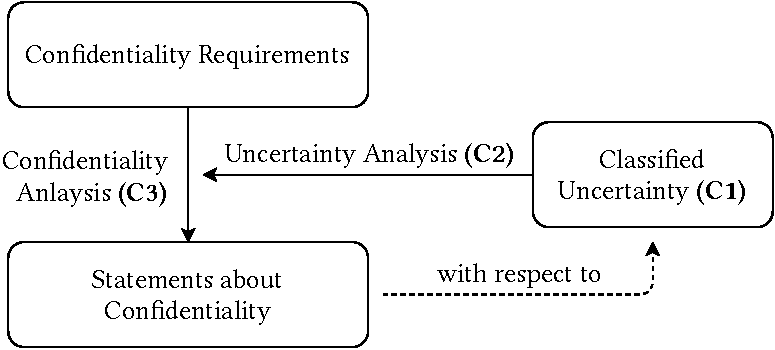
\includegraphics[width=0.75\textwidth]{figures/chapter1/approach.pdf}
    \caption{Schematic and informal visualization of the presented approach.}
    \label{fig:introduction:approach}
\end{figure}

\paragraph{Classifying Uncertainty}
Classifying uncertainty provides the required terminology to inspect and assess uncertainty regarding confidentiality.
By identifying relevant uncertainty types and grouping uncertainty sources into classes, we bootstrap the further analysis process.
This part also includes considering the identification of uncertainty sources by addressing the lack of awareness and expert knowledge of software architects.
Put simply, we first have to investigate the nature of the problem before developing a solution.
This represents an answer to \RQ{1} and also our first Contribution \C{1}.


\paragraph{Uncertainty Analysis}
We build on these findings on the types and attributes of uncertainty sources that affect the confidentiality of a software system to develop an analysis of uncertainty.
Here, we first define an impact analysis to propagate uncertainty.
Based on the relations of the elements of a software architecture, we propagate the effects of uncertainty sources on confidentiality through the architectural model.
Comparable to change impact analysis \cite{heinrich_methodology_2018,busch_architecture-based_2020,rostami_architecture-based_2015}, this analysis yields an impact set that predicts the potential impact of unanticipated change, i.e., uncertainty.
This does not only serve software architects as an early prediction but also shows the effects of uncertainty sources that can subsequently be used in confidentiality analysis.
Put simply, we have to analyze uncertainty first before analyzing confidentiality under uncertainty.
This represents an answer to \RQ{2} and also our second Contribution \C{2}.


\paragraph{Confidentiality Analysis}
Confidentiality analyses take confidentiality requirements as input to make statements about the confidentiality of a software architecture, see \autoref{fig:introduction:approach}.
Based on our previous findings, we extend existing analysis approaches \cite{seifermann_detecting_2022,boltz_extensible_2024} to consider uncertainty.
Here, black-box \cite{walter_architectural_2022} and white-box \cite{hahner_model-based_2023} analysis extensions are possible.
After software architects have modeled sources of uncertainty as part of the architecture model, the uncertainty analysis determines which confidentiality requirements are violated due to which uncertainties.
Here, considering multiple interacting uncertainty sources is especially challenging, as their effects can add up or cancel each other out \cite{camara_uncertainty_2022,camara_addressing_2022}.
This represents an answer to \RQ{3} and also our third Contribution \C{3}.

As discussed previously, all contributions can be used independently or in conjunction.
We also provide tooling that supports the modeling and the analysis based on established frameworks \cite{reussner_modeling_2016,reussner_palladio_2024}.
In this thesis, we motivate, present, and evaluate all contributions independently.
We transparently enumerate assumptions and limitations.
Last, we provide a comprehensive data set including our tooling and all raw evaluation data \cite{dataset}.




\section{Outline and Reading Paths}%
\label{sec:introduction:outline}

This dissertation consists of four parts: The prolog, the contributions, their validation, and the epilog.
The remainder of the prolog comprises the presentation of foundations in \autoref{ch:foundations} and the introduction of a running example in \autoref{ch:runningexample}.
This running example does not only serve to exemplify the scientific problems addressed in this thesis, but will also be used intensively throughout the thesis.
Afterward, we present the contributions of this dissertation.
We start with an overview that continues the introduction of our approach in \autoref{ch:overview}.
Then, we introduce our classification of uncertainty (\C{1}) in \autoref{ch:classification}, the uncertainty impact analysis (\C{2}) in \autoref{ch:impactanalysis}, and four uncertainty-aware confidentiality analysis approaches (\C{3}) in \autoref{ch:confidentialityanalysis}.
We show the scenarios used in the validation of the contributions in \autoref{ch:evaluationscenarios} and present our comprehensive evaluation thereafter in \autoref{ch:evaluation}.
Last, the epilog concludes this thesis with an overview of related work in \autoref{ch:relatedwork} and a summary and outlook on future work in \autoref{ch:conclusion}.
We would also like to point out the additional information in the \hyperref[ch:appendix]{Appendix} and in the data set \cite{dataset}.
There are multiple ways to read this dissertation:

\begin{itemize}
    \item[\faChevronCircleRight] \textbf{Beginner readers}, who are not interested in the technical details of the contributions but want to understand the bigger picture, continue with reading the foundations in \autoref{ch:foundations}.
    Afterward, every chapter ends with a section called \emph{In Simpler Words}.
    There, we explain the most important concepts and findings of each chapter without using scientific terminology but with reference to everyday life.
    For your convenience, this means Sections \ref{sec:introduction:simple}, \ref{sec:foundations:simple}, \ref{sec:runningexample:simple}, \ref{sec:overview:simple}, \ref{sec:classification:simple}, \ref{sec:impactanalysis:simple}, \ref{sec:confidentialityanalysis:simple}, \ref{sec:evaluationscenarios:simple}, \ref{sec:evaluation:simple}, \ref{sec:relatedwork:simple}, and \ref{sec:conclusion:simple}\footnote{%
    This dissertation is meant to be read digitally.
    We make extensive use of references, e.g., between chapters or enumerable items like research questions, contributions, and evaluation goals.
    We recommend using a shortcut to jump back from following a reference.
    Furthermore, all paragraphs, figures, and tables are optimized for the DIN A4 version of this dissertation.
    If you happen to have the DIN A5 or the book version at hand, you can find the other versions until the link expires at \url{https://thesis.abunai.dev/}.}.

    \item[\faChevronCircleRight] \textbf{Expert readers}, who want to gain an overview of our insights, will find gray highlighted boxes titled \emph{Findings} throughout the thesis.
    A concise yet technical overview of the contributions is given in \autoref{ch:overview}, and the conclusion in \autoref{ch:conclusion} provides a summary.
    If the information provided there is not sufficient, the contribution chapters \ref{ch:classification}, \ref{ch:impactanalysis}, and \ref{ch:confidentialityanalysis} come with their own introduction and summary sections.

    \item[\faChevronCircleRight] \textbf{Particularly interested readers} are welcome to read the entire work in one piece.
    Furthermore, we recommend suitable basic literature in \autoref{ch:foundations} and provide all relevant references to own publications at the beginning of each chapter.
\end{itemize}





\section{Summary and Outlook}%
\label{sec:introduction:summary}

In this chapter, we introduced the topic of this thesis.
First, we motivated the actuality and relevance of confidentiality, uncertainty, and software architecture.
Without considering uncertainty as a first-class concern within the software architecture, the validity of statements about confidentiality can be degraded or completely voided \cite{hahner_dealing_2021}.
Afterward, we presented three challenges of architecture-based and uncertainty-aware confidentiality analysis.
They revolve around understanding the relationship between uncertainty and confidentiality, representing uncertainty in architectural models, and providing automated analyses. 
The challenges of representing and analyzing uncertainty in the software architecture are also supported by the literature \cite{troya_uncertainty_2021,hezavehi_uncertainty_2021}.
We summarized these challenges in our problem statement as \emph{inspection problem} (\PR{0}{1}) and \emph{assessment problem} (\PR{0}{2}).

Based on these problems, we presented our research goal and three research questions that map to the three Contributions \C{1} -- \C{3} of this dissertation.
First, we define a novel classification of uncertainty regarding confidentiality.
Second, we use this classification in uncertainty impact analysis, thereby propagating the effects of uncertainty within the software architecture and calculating the potential impact.
Third, we include the impact of uncertainty within confidentiality analysis to identify confidentiality violations with respect to uncertainty.
We summarized the relations of these research questions and our contributions by introducing this dissertation's approach.
Last, we presented the outline and the intended reading paths for the different types of readers of this thesis.

Next, in \readingpath{ch:foundations}, we explain the foundations required for understanding this thesis, e.g., \acp{DAG}, or \ac{MDSD}.
Afterward, we introduce the running example of this thesis in \readingpath{ch:runningexample}.
Both chapters also help to understand the context and the general assumptions of this dissertation.
In \readingpath{ch:overview}, we continue the presentation of our approach by relating common activities in the procedure of handling uncertainty in software architectures to our contributions and our tool support.





\section{In Simpler Words}%
\label{sec:introduction:simple}

Our world runs on data.
Think of social media, online shopping, advertisement, smart home, or artificial intelligence---all of these systems require large amounts of data to provide their functionality.
In this dissertation, we focus on the confidentiality of this data.
Confidentiality demands that data is not shown to unauthorized persons or organizations.
It is a quality property of software systems and is related to security and privacy.
In this dissertation, we research how to analyze the confidentiality of software systems while considering uncertainty.
Put simply, uncertainty is the lack of knowledge, i.e., not knowing something for sure, e.g., because an engineer cannot assess environmental conditions or the behavior of third parties.

We present an approach to better understand the potential impact of uncertainty on confidentiality by using a high-level view of the software system, i.e., software architecture, the big picture of a software system.
Therefore, we first have to better understand uncertainty---like you need to understand the rules of a board game to be able to play better.
Afterward, we build an analysis that propagates uncertainty within a software architecture to better understand its impact.
This is comparable to introducing a drop of dye into a stream of water and then observing the coloration.
In the end, we enable software architects to identify confidentiality violations early and to build better software systems that protect the data of their users.

\chapter{Foundations}%
\label{ch:foundations}%


In this chapter, we explain the foundations of this thesis.
As stated in the title, the topic of this thesis revolves around software architecture, confidentiality, and uncertainty.
We present common terminology, approaches, and underlying concepts that will be used throughout this thesis.
For every section, we also provide references for further reading.

The remainder of this chapter is structured as follows:
First, we introduce the central concerns of this thesis, i.e., uncertainty, and confidentiality.
Afterward, we explain the concept of model-driven development and how we use it in architectural modeling and analysis.
Last, we present the foundations of modeling data flows of software systems.





\section{Uncertainty}%
\label{sec:foundations:uncertainty}

Uncertainty has many definitions:
\textcite{walker_defining_2003} refer to uncertainty as \enquote{being any departure from the unachievable ideal of complete determinism} \cite{walker_defining_2003}.
\textcite{weyns_introduction_2020} defines uncertainty as \enquote{any deviation of deterministic knowledge that may reduce the confidence of adaptation decisions made based on the knowledge} \cite{weyns_introduction_2020}.
In architecture evaluation, \textcite{sobhy_evaluation_2021} define it as \enquote{the lack of full knowledge about the outcomes of deploying the architecture options} \cite{sobhy_evaluation_2021}.
Uncertainty is also related to doubt, error \cite{jcgm_1002008_evaluation_2008}, or risk \cite{international_organization_for_standardization_isoiec_2018}.
In the ISO/IEC 27000 standard, uncertainty is defined as \enquote{the state, even partial, of deficiency of information related to, understanding or knowledge of, an event, its consequence, or likelihood} \cite{international_organization_for_standardization_isoiec_2018}.
The current version of the \acf{OMG} \acf{PSUM} standard refers to \textcite{zhang_understanding_2016}, describing uncertainty as \enquote{the lack of confidence (i.e., knowledge) about the timing and nature of inputs, the state of a system, a future outcome, as well as other relevant factors} \cite{PSUM}.
In software design, the \emph{cone of uncertainty} describes the lack of knowledge about a software system in early development phases \cite{mcconnell_software_1998}.
Here, uncertainty about open design decisions can impact cost estimation.

These definitions share four common aspects.
First, they refer to a lack of information regarding a system.
Second, they mention sources of uncertainty within the system or its environment \cite{acosta_uncertainty_2022}.
Third, they name consequences of uncertainty, e.g., increased risk, which may impact the quality of the system.
Fourth, the majority of these definitions consider even small changes in certainty, using terms like \enquote{any deviation}, \enquote{full knowledge}, or \enquote{unachievable ideal}, highlighting how omnipresent or ubiquitous uncertainty is.
For the scope of this thesis, we adopt these four aspects and refer to uncertainty as the commonly occurring lack of information that can negatively impact the quality of a software system.

Existing literature proposes different approaches to deal with uncertainty, involving activities like identification, management, and mitigation \cite{PSUM,weyns_introduction_2020,perez-palacin_dealing_2014,perez-palacin_uncertainties_2014,sobhy_evaluation_2021,hezavehi_uncertainty_2021}.
Another common approach to uncertainty is its classification, resulting in a multitude of taxonomies \cite{bures_capturing_2020,esfahani_uncertainty_2013,mahdavi-hezavehi_classification_2017,perez-palacin_uncertainties_2014,ramirez_taxonomy_2012,walker_defining_2003,armour_five_2000,troya_uncertainty_2021,hezavehi_uncertainty_2021,PSUM}.
These taxonomies describe many dimensions that shall help to better understand uncertainty, e.g., by distinguishing between sources of uncertainty or classifying the size of the knowledge gap.
Examples of such uncertainties are the lack of knowledge of the structure of a software system, the behavior of external systems, or a sensor's input value.
At the time of writing, uncertainty represents a commonly researched topic with novel findings and challenges ahead \cite{weyns_towards_2023}.

In the following, we give an overview of the current state of classifying and describing uncertainty.
We investigated existing taxonomies \cite{bures_capturing_2020,esfahani_uncertainty_2013,mahdavi-hezavehi_classification_2017,perez-palacin_uncertainties_2014,ramirez_taxonomy_2012,walker_defining_2003,armour_five_2000}, as well as recent \acfp{SLR} and surveys on uncertainty \cite{troya_uncertainty_2021,hezavehi_uncertainty_2021} and the most recent version of the \ac{OMG} \ac{PSUM} standard \cite{PSUM}, which is in beta status.
To unify the terminology, we only use the terms \emph{classification}, \emph{category}, and \emph{option}.


\begin{table}
    \begin{tabularx}{\textwidth}{p{3.8cm}X}
        \toprule
        Available Categories & Available Options \\
        \midrule
        \category{Location}{Describes where uncertainty originates from or where it manifests itself within the system or model \cite{bures_capturing_2020,mahdavi-hezavehi_classification_2017,perez-palacin_uncertainties_2014,walker_defining_2003,troya_uncertainty_2021,PSUM}} 
        \optionlist{
            \option{Context}{system boundaries \cite{perez-palacin_uncertainties_2014,walker_defining_2003}, user input \cite{bures_capturing_2020}, execution context \cite{mahdavi-hezavehi_classification_2017,PSUM}, environment \cite{PSUM}}
            \option{Model structural}{existence of elements \cite{troya_uncertainty_2021}, elements and their relationship \cite{walker_defining_2003,perez-palacin_uncertainties_2014}, structural differences \cite{mahdavi-hezavehi_classification_2017}, components and their properties \cite{bures_capturing_2020}}
            \option{Model technical}{software and hardware \cite{walker_defining_2003}}
            \option{Input}{input types \cite{walker_defining_2003}, input values \cite{perez-palacin_uncertainties_2014}, measurement deviation \cite{troya_uncertainty_2021,PSUM}, geographical location \cite{PSUM}, time \cite{PSUM}}
            \option{Parameters}{parameter calibration \cite{walker_defining_2003,perez-palacin_uncertainties_2014}}
            \option{System behavior}{actual behavior \cite{bures_capturing_2020}, including parameters and actions \cite{troya_uncertainty_2021}}
            \lastoption{Belief}{uncertain statements about system and environment \cite{troya_uncertainty_2021}}
        }
        \category{Level}{Describes how much is known about the uncertain influence and how the uncertainty can be described \cite{walker_defining_2003,mahdavi-hezavehi_classification_2017,perez-palacin_uncertainties_2014,bures_capturing_2020,armour_five_2000,PSUM}}
        \optionlist{
            \option{Statistical}{Statistical data available \cite{walker_defining_2003,mahdavi-hezavehi_classification_2017}}
            \option{Scenario}{Possible scenarios available without statistical data \cite{walker_defining_2003,mahdavi-hezavehi_classification_2017,armour_five_2000}}
            \option{Recognized ignorance}{Awareness of uncertainty, but cannot be further described \cite{walker_defining_2003}, can be supported by evidence, e.g., empirical evidence, or theorem proving results \cite{PSUM}}
            \option{Total ignorance}{Lack of awareness of uncertainty \cite{walker_defining_2003}}
            \option{Orders of Uncertainty}{No uncertainty (0th), known uncertainty (1st), lack of awareness, i.e., unknown unknowns (2nd), lack of awareness and process (3rd), meta-uncertainty (4th) \cite{armour_five_2000,bures_capturing_2020,perez-palacin_uncertainties_2014}}
            \lastoption{Perspective}{Subjective, based on observation, or objective, independent of any observing agency \cite{PSUM}}
        }
        \bottomrule
    \end{tabularx}
    \caption{Categories and options to classify the location and level of uncertainty.}%
    \label{table:foundations:sources:locationlevel}
\end{table}

\autoref{table:foundations:sources:locationlevel} shows the first two available categories regarding the \emph{location} and the \emph{level} and all available options.
Uncertainty is often described with its \emph{location} which describes where the uncertainty manifests itself.
Many classifications provide options like context, input, or behavior.
The \emph{level} category is used to describe how much is known about the uncertainty.
Here, three different approaches exist.
Some classifications define the level based on the description of uncertainty, e.g., by using statistical means, or scenarios \cite{mahdavi-hezavehi_classification_2017}.
Others refer to the orders of uncertainty \cite{armour_five_2000} and the distinction between known unknowns and unknown unknowns.
However, even in this order, different nuances exist, e.g., recognized ignorance compared with statistical data.
Last, the level can be described based on the perspective being subjective or objective \cite{PSUM}.


\begin{table}
    \begin{tabularx}{\textwidth}{p{3.6cm}X}
        \toprule
        Available Categories & Available Options \\
        \midrule
        \category{Nature}{Describes the essence and character of the uncertainty \cite{bures_capturing_2020,mahdavi-hezavehi_classification_2017,perez-palacin_uncertainties_2014,walker_defining_2003,troya_uncertainty_2021,PSUM}}
        \optionlist{
            \option{Aleatory}{Uncertainty due to inherent variability or randomness \cite{bures_capturing_2020,mahdavi-hezavehi_classification_2017,perez-palacin_uncertainties_2014,walker_defining_2003,troya_uncertainty_2021,PSUM}}
            \lastoption{Epistemic}{Uncertainty due to a lack of knowledge \cite{bures_capturing_2020,mahdavi-hezavehi_classification_2017,perez-palacin_uncertainties_2014,walker_defining_2003,troya_uncertainty_2021,PSUM}, can be further described as indeterminacy, e.g., due to insufficient resolution, or missing information \cite{PSUM}}
        }
        \category{Manageability}{Describes whether the uncertainty can be reduced \cite{esfahani_uncertainty_2013,walker_defining_2003,PSUM}}
        \optionlist{
            \option{Reducible}{Uncertainty can be fully reduced after acknowledgement \cite{esfahani_uncertainty_2013,walker_defining_2003,PSUM}}
            \option{Partially reducible}{No full certainty, but uncertainty can be reduced \cite{PSUM}}
            \lastoption{Irreducible}{Uncertainty cannot be further reduced at this point in time \cite{esfahani_uncertainty_2013,walker_defining_2003,PSUM}}
        }
        \category{Emerging time}{Describes at which state of the software development uncertainty arises \cite{hezavehi_uncertainty_2021,mahdavi-hezavehi_classification_2017,troya_uncertainty_2021,perez-palacin_uncertainties_2014,ramirez_taxonomy_2012,PSUM}}
        \optionlist{
            \option{Requirements time}{As requirements are defined \cite{ramirez_taxonomy_2012,troya_uncertainty_2021}}
            \option{Design time}{As the software system is designed \cite{ramirez_taxonomy_2012,hezavehi_uncertainty_2021,troya_uncertainty_2021,mahdavi-hezavehi_classification_2017}}
            \option{Verification}{At verification of software models \cite{troya_uncertainty_2021}}
            \option{Testing}{During software testing \cite{hezavehi_uncertainty_2021,troya_uncertainty_2021}}
            \option{Implementation}{As the software gets implemented \cite{troya_uncertainty_2021}}
            \lastoption{Run time}{During software execution \cite{hezavehi_uncertainty_2021,mahdavi-hezavehi_classification_2017,troya_uncertainty_2021,perez-palacin_uncertainties_2014,ramirez_taxonomy_2012}, can be described using patterns like periodic, persistent, or random \cite{PSUM}}
        }
        \bottomrule
    \end{tabularx}
    \caption{Categories and options to classify the nature, manageability, and emerging time of uncertainty.}%
    \label{table:foundations:sources:naturemanagetime}
\end{table}

\autoref{table:foundations:sources:naturemanagetime} shows the categories regarding the \emph{nature}, \emph{manageability}, and \emph{emerging time}.
The \emph{nature} of uncertainty with the two options \emph{aleatory} and \emph{epistemic} represents the most uniformly used category among all classifications.
However, this category is questioned \cite{esfahani_uncertainty_2013,kiureghian_aleatory_2009} as it depends on the point of view and is often not clearly distinguishable.
Thus, some use the category \emph{manageability} that focuses on reducibility.
The distinction between reducible, partially reducible and irreducible is also supported by the \ac{PSUM} standard.
The category \emph{emerging time} describes the time when uncertainty arises.
The options reflect the common phases of software engineering from requirements time to run time.


\begin{table}
    \begin{tabularx}{\textwidth}{p{4cm}X}
        \toprule
        Available Categories & Available Options \\
        \midrule
        \category{Impact on Quality}{Describes how uncertainty affects quality properties \cite{hezavehi_uncertainty_2021,PSUM}}
        \optionlist{
            \option{Performance}{Impact on performance \cite{hezavehi_uncertainty_2021}}
            \option{Resources}{Impact on resource consumption \cite{hezavehi_uncertainty_2021}}
            \option{Safety}{Impact on a system's safety \cite{hezavehi_uncertainty_2021}}
            \lastoption{Risk}{General effect of uncertainty on system objectives \cite{PSUM}}
        }
        \category{Relationship}{The relation between uncertainties \cite{ramirez_taxonomy_2012,PSUM}}
        \optionlist{
            \option{Directed}{Directed relationship or influences between uncertainties \cite{ramirez_taxonomy_2012}}
            \option{Related}{Unspecified relationship between uncertainties \cite{ramirez_taxonomy_2012}}
            \lastoption{Effect}{An uncertainty can be caused by another uncertainty \cite{PSUM}}
        }
        \category{Source}{Potential sources of uncertainty \cite{perez-palacin_uncertainties_2014,esfahani_uncertainty_2013,mahdavi-hezavehi_classification_2017,ramirez_taxonomy_2012,PSUM}}
        \optionlist{
            Several publications contain comprehensive lists of uncertainty sources, e.g., human in the loop \cite{perez-palacin_uncertainties_2014}, abstraction \cite{perez-palacin_uncertainties_2014}, missing requirements \cite{ramirez_taxonomy_2012}, inadequate design \cite{ramirez_taxonomy_2012}, \dots
        }
        \bottomrule
    \end{tabularx}
    \caption{Categories and options to classify the impact on quality, relationship, and source of uncertainty.}%
    \label{table:foundations:sources:impactrelationsource}
\end{table}

\autoref{table:foundations:sources:impactrelationsource} shows the categories regarding the \emph{impact on quality}, \emph{relationship} of uncertainty, and uncertainty \emph{sources}.
The \emph{impact on quality} is important as not all uncertainties affect a system's quality.
The \emph{relationship} of uncertainty represents influences of one uncertainty source to another.
Last, several publications list \emph{sources} of uncertainty as not all taxonomies directly aim at classifying sources. 
We list some examples here and also provide a comprehensive catalog of sources as part of the thesis' data set \cite{dataset}.

\furtherreading{For a comprehensive introduction to the topic of uncertainty in \acfp{SAS}, we recommend \textcite{weyns_introduction_2020}.
A more recent overview of the research community is given by \textcite{hezavehi_uncertainty_2021}.}





\section{Confidentiality}%
\label{sec:foundations:confidentiality}

Confidentiality is defined as the \enquote{property that information is not made available or disclosed to unauthorized individuals, entities, or processes} \cite{international_organization_for_standardization_isoiec_2018}.
It is named together with integrity and availability as part of information security \cite{international_organization_for_standardization_isoiec_2018}.
It is also often referred to in the context of privacy \cite{schaar_privacy_2010,sulochana_preserving_2015,boltz_modeling_2024,boltz_model-based_2022}.
Confidentiality requirements specify what should be accessible by whom.
Properties of such requirements are, for instance, stakeholders, the protected data, and the purpose \cite{onabajo_properties_2006}.
Confidentiality is part of legal regulations such as the \acf{GDPR} \cite{council_of_european_union_regulation_2016}.
Exemplary confidentiality requirements are the protection of personal information or payment data \cite{boltz_extensible_2024}.

Common mechanisms to ensure confidentiality are access control and data encryption \cite{schumacher_security_2013}.
Access control provides \enquote{means to ensure that access to assets is authorized and restricted based on business and security requirements} \cite{international_organization_for_standardization_isoiec_2018}.
For instance, \acf{RBAC} uses the member roles of an organization to specify permissions.
An example is that only members with the administrative role shall be able to directly access a database.
\acf{ABAC} extends this and supports the evaluation of complex rules comprising different attributes \cite{hu_guide_2014}.
The \acf{XACML} extends the \acf{XML} and represents an open industry standard to formulate and enforce \ac{ABAC} policies \cite{oasis_extensible_2013}.
Encryption is the mapping of a readable plain text to an unreadable cipher text, using an encryption algorithm and a key \cite{bauer_encryption_2005}.
Without knowing the key, the plain text shall be hard or impossible to determine.
In sum, both mechanisms help to prevent the access of unauthorized entities to protected data and thus help to ensure confidentiality. 

\furtherreading{\textcite{schumacher_security_2013} provides a comprehensive introduction to security in the development of software systems, covering an overview of the field of security and a variety of security patterns.}



\section{Model-Driven Software Development}%
\label{sec:foundations:mds}

\begin{figure}[b]
    \centering
    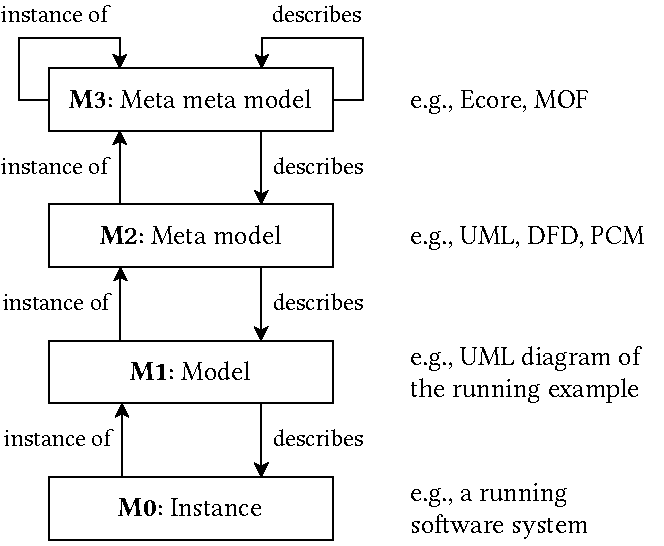
\includegraphics[width=0.65\textwidth]{figures/chapter2/metalevels.pdf}
    \caption{The four meta levels with examples from our domain, based on \textcite{stahl_model-driven_2006}.}
    \label{fig:foundations:metalevels}
\end{figure}

\acf{MDSD} is a concept where models play a central role in the development of software systems \cite{stahl_model-driven_2006}.
Nowadays, using models in software development is common, e.g., as shown by the popularity of the \acf{UML}.
However, compared to only using models for documentation purposes, model-driven approaches give models an equivalent or higher importance than code.
This includes techniques like tailored modeling languages, model transformations, and code generation.
This thesis uses design time models for analysis purposes, which is related to \ac{MDSD}.

\textcite{stachowiak_allgemeine_1973} names three central properties of models: representation, abstraction, and pragmatics.
First, a model represents the modeled entity, e.g., a \ac{UML} diagram can represent the structure or behavior of a real software system.
Second, a model abstracts from the modeled entity, e.g., a \ac{UML} activity diagram does not represent every single line of code.
Third, a model has pragmatics, it follows a purpose.
The models we use are generally about representing a software system in a simplified yet analyzable way.

One of the most important aspects of \ac{MDSD} is meta modeling.
A meta model describes the structure of a model, including available elements, their relationship, and modeling constraints \cite{stahl_model-driven_2006}.
Put simply, a meta model states the rules on how a model has to be constructed.
An example is the \ac{UML} providing many diagram types like activity diagrams, class diagrams, or deployment diagrams.
The meta model itself can be described following the same concept using a meta meta model, which states the rules of the meta model.
Common meta meta models are the \ac{OMG} \acf{MOF} \cite{omg_about_2016} and Ecore from the \acf{EMF} \cite{steinberg_emf_2008}.
Due to the high level of abstraction, these models can describe themselves.
This is visualized in \autoref{fig:foundations:metalevels}.
There, we depict the description and instance relation of all meta levels and show examples from the domain of this thesis, e.g., Ecore, the \ac{UML} meta model, and \ac{UML} models.
This includes the instance level, representing an entity of the real world, e.g., the modeled software system.

\furtherreading{We recommend the comprehensive introduction to \acf{MDSD} by \textcite{stahl_model-driven_2006}.}





\section{Software Architecture}%
\label{sec:foundations:architecture}

As stated in the title of this thesis, this work uses the architectural representation of software systems as a baseline.
Software architecture comprises the \enquote{fundamental concepts or properties of a system in its environment embodied in its elements, relationships, and in the principles of its design and evolution} \cite{international_organization_for_standardization_isoiecieee_2022}, according to the ISO/IEC/IEEE 42010 standard.
Software architecture can be also interpreted as a set of \acfp{ADD} \cite{jansen_architectural_2008,jansen_software_2005}.
Another approach to software architecture is to describe it by its views, e.g., a logical view, or a development view \cite{kruchten_41_1995}.
As discussed in the previous section, we used model-driven techniques.
Here, \acfp{ADL} provide \enquote{means of expression, with syntax and semantics, consisting of a set of representations, conventions, and associated rules intended to be used to describe an architecture} \cite{international_organization_for_standardization_isoiecieee_2022}.
As a meta model for this work, we use the \acf{PCM} \cite{reussner_modeling_2016}, which we describe in more detail in the following.

The Palladio approach \cite{reussner_modeling_2016} enables modeling, simulating, and analyzing software architectures regarding quality dimensions like performance, reliability, or maintainability.
Besides comprehensive tool support \cite{reussner_palladio_2024}, the approach provides a meta model for software architecture, the \ac{PCM} \cite{reussner_palladio_2011,reussner_modeling_2016}.
Palladio builds on the concept of \acf{CBSE}, which divides software architectures into reusable and composable components.
The \ac{PCM} meta model has been used previously in security analysis, e.g., regarding confidentiality \cite{seifermann_architectural_2022}, access control analysis \cite{pilipchuk_architectural_2021}, or attacker propagation \cite{walter_context-based_2023}.
Here, the shared underlying meta model simplifies the reuse of architectural models, which minimizes costs.
The \ac{PCM} is partitioned into five submodels:

\begin{itemize}
    \item The \emph{Component Repository Model} contains components and interfaces.
    The components' behavior is described using \acfp{SEFF} that abstract from the control flow.
    Components can be composed both vertically, and horizontally.
    The repository belongs to the structural viewpoint.
    The inter-component behavior description with \acp{SEFF} belongs to the behavioral viewpoint.
    For instance, components could be the user management or database of an online learning platform.
    \item The \emph{System Model} describes the assembly, i.e., the wiring of the components of the \emph{Component Repository Model}.
    This belongs to the structural viewpoint.
    For instance, the previously introduced user management component could be wired to the database component for the persistence of user data.
    \item The \emph{Execution Environment Model} defines hardware resources and the network.
    These resources represent the deployment locations of components.
    For instance, resources can be an on-premise server or a cloud service.
    \item The \emph{Component Allocation Model} describes the deployment of assembly contexts that represent components from the system model, i.e., shows the allocation of the components in use.
    This model belongs to the deployment viewpoint.
    For instance, the database component can be deployed on-premise.
    \item The \emph{Usage Model} specifies the user interaction with the software system.
    By modeling expected calls to the components, usage scenarios can be expressed.
    For instance, users interact with the user management when registering on the online platform.
\end{itemize}

In sum, the \ac{PCM} enables the system-independent modeling of components and their behavior and of the executing environment.
Furthermore, engineers describe the system-specific assembly context and the allocation context of the components, and also the usage context of the software system.
Based on these submodels, a multitude of simulations can be executed in the Palladio Bench \cite{reussner_palladio_2024}.
For instance, using the information on expected usage scenarios together with the allocation of components, performance bottlenecks can be identified.
For the sake of this thesis, we only focus on confidentiality.
Thus, we build on the \ac{PCM} as comprehensive \ac{ADL} without relating to other analysis approaches of different quality dimensions like performance and reliability.

We choose the \ac{PCM} as foundation of our work due to its maturity, wide adoption, and reception in the community \cite{koziolek_tracing_2022}.
However, we want to stress that the contributions presented in this dissertation can also be realized with other \acp{ADL}, e.g., the \ac{UML}.
Here, using the \ac{PCM} does not represent a \enquote{vendor lock-in}, as its meta models are related to other well-known diagram types like \ac{UML} component diagrams or \ac{UML} activity diagrams.

\furtherreading{\textcite{reussner_modeling_2016} present the Palladio approach in detail.
Additionally, they provide an overview of software architecture as a discipline with a focus on architectural modeling and analysis.}





\section{Data Flow Diagrams}%
\label{sec:foundations:dfd}

\textcite{demarco_structure_1979} introduces \acfp{DFD} to represent software systems \enquote{from the point of view of the data} \cite{demarco_structure_1979}.
By focusing on data flows instead of control flows, the data-oriented analysis of issues within software systems is simplified.
Regarding security analysis, \acp{DFD} represent a simple yet powerful representation of software systems \cite{schneider_how_2024}.
They are used both for documentation and discussion \cite{sion_security_2020,schneider_how_2024}, and also automated analysis \cite{alshareef_precise_2022,seifermann_detecting_2022,canfora_data_1992,berger_automatically_2016,tuma_flaws_2019,tuma_automating_2020}.
Especially regarding confidentiality, the use of \acp{DFD} is expedient, as \enquote{problems tend to follow the data flow, not the control flow} \cite{shostack_threat_2014}.
In the following, we briefly introduce the original syntax of \acp{DFD} \cite{demarco_structure_1979}.
Afterward, we introduce the unified modeling primitives for \acp{DFD} \cite{seifermann_unified_2021}, used throughout this thesis, and the representation of \acp{DFD} as directed graphs \cite{diestel_graph_2017,bang-jensen_digraphs_2009}.

\furtherreading{For a historically relevant, original definition of \acfp{DFD}, we refer to \textcite{demarco_structure_1979}.
To learn more about the fundamentals, see the introduction to graph theory by \textcite{diestel_graph_2017}.}


\subsection{Elements of Data Flow Diagrams}

In describing the conventions of data flow diagrams, \textcite{demarco_structure_1979} states that \enquote{the data flow diagram shows flow of data, not of control} \cite{demarco_structure_1979}.
Resulting from this, loops are excluded from \acp{DFD} as they represent control flow, of which \enquote{the data are unaware of} \cite{demarco_structure_1979}.
The graphical notation of \acp{DFD} comprises four elements:

\begin{itemize}
    \item \emph{Data sources and sinks} are represented by boxes.
    They depict an entity like a person or an organization that is outside of the context of the system under study.
    Examples are the user of a software system or an external data base.
    \item \emph{Processes} are represented by circles.
    They depict the processing or transformation of data within the scope of the system under study.
    Examples are the processing of user input or the calculation of results.
    \item \emph{Files} are represented by straight line.
    They depict internal and temporary repositories of data within the scope of the system under study.
    An example is the temporary storage of intermediate data processing results.
    \item \emph{Data flows} are represented by named arrows.
    They represent data paths or pipelines of data within the software system and connect all other elements.
    Multiple arrows between two elements are possible if the data flow has more than one purpose or type.
    Examples are the flow of data from a source or the flow between two processes.
\end{itemize}

\begin{figure}[b]
    \centering
    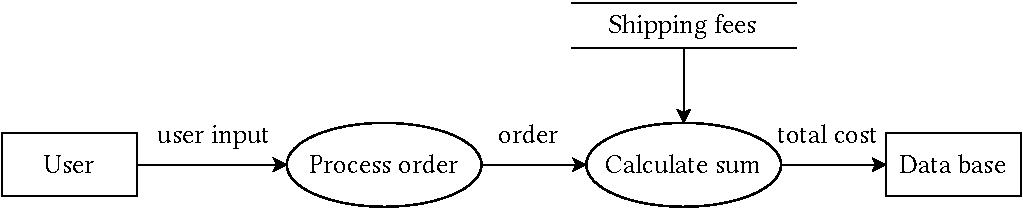
\includegraphics[width=\textwidth]{figures/chapter2/dataflowdiagram.pdf}
    \caption{A \acf*{DFD} showing all four element types in a simplified online shop scenario.}
    \label{fig:foundations:dataflowdiagram}
\end{figure}

\autoref{fig:foundations:dataflowdiagram} shows the \ac{DFD} of a simplified online shop scenario.
The \emph{User} represents a data source, the \emph{Data base} represents a data sink, the \emph{Shipping fees} represent internal storage, and the internal processing represents processes.
All elements are connected by named arrows, i.e., data flows.
The user input comprising an order from the shop is first processed.
Afterward, the total cost of the order is calculated, which includes applying the correct shipping fee.
The result is stored in the data base.
This figure shows several conventions of \textcite{demarco_structure_1979}, e.g., the arrows of files have no description as their purpose is unambiguous.
Inspired by related work \cite{seifermann_architectural_2022}, we use two horizontal lines to represent files throughout this thesis to increase readability.


\subsection{Unified Modeling Primitives}

The \ac{DFD} syntax is simple and easy to understand.
However, this simplicity causes ambiguity, especially regarding security analysis.
\textcite{sion_security_2020} name several weaknesses of \acp{DFD} for security-related analysis:
They lack the means to represent security concepts, lack precision in describing the details of flowing data, and do not express deployment information.
To address this, \textcite{seifermann_unified_2021} present the \emph{unified modeling primitives} of \acp{DFD} by combining multiple notations of security-focussed \ac{DFD} notations from other work \cite{seifermann_data-driven_2019,tuma_flaws_2019}.
We use these primitives in this thesis to represent \acp{DFD}.

\begin{figure}
    \centering
    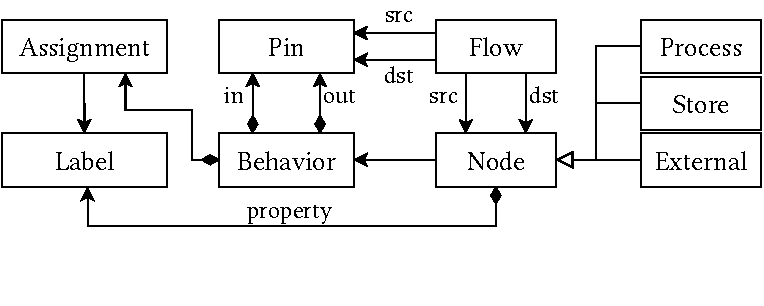
\includegraphics[width=0.85\textwidth]{figures/chapter2/unifiedmodelingprimitives.pdf}
    \caption{Meta model of unified modeling primitives, based on \textcite{seifermann_unified_2021}.}
    \label{fig:foundations:unifiedmodelingprimitives}
\end{figure}

\autoref{fig:foundations:unifiedmodelingprimitives} shows the meta model of the unified modeling primitives.
It comprises the element types known from \acp{DFD} by \textcite{demarco_structure_1979}, i.e., \emph{External} nodes, \emph{Processes}, and internal \emph{Stores}.
These \emph{Nodes} are connected by \emph{Flows}.
To reduce the ambiguity of data flows, \emph{Pins} are used to represent the incoming and outgoing data of a \emph{Node}.
Alternative \emph{Pins} can be used to represent required inputs, e.g., the calculation of the sum in \autoref{fig:foundations:dataflowdiagram} requires both the order and the shipping fees.
Multiple ingoing flows to a single \emph{Pin}, or multiple outgoing flows from a single \emph{Pin} represent alternative flows.
\emph{Pins} are used to decouple the \emph{Behavior} from a \emph{Node}.
A \emph{Behavior} describes the data processing of a node using \emph{Assignments}.
\emph{Assignments} alter \emph{Labels} that represent characteristics of flowing data, e.g., whether data is encrypted or personal.
For instance, the order processing in \autoref{fig:foundations:dataflowdiagram} removes all personal information of the user and only forwards the cost of purchased items, which can be represented using an \emph{Assignment} within the \emph{Behavior} of the \emph{Process}.
This addresses the shortcoming regarding behavior descriptions \cite{sion_security_2020}.
Last, \emph{Labels} are used to describe the properties of \emph{Nodes}, e.g., their deployment.

Using the unified modeling primitives, we can analyze transitive data flows by tracing \emph{Labels} in \acp{DFD}.
The procedure of following \emph{Labels} through the system is called \emph{label propagation} \cite{seifermann_architectural_2022,seifermann_unified_2021,seifermann_detecting_2022}.
To identify confidentiality violations, the propagated \emph{Labels} can be compared to the property \emph{Labels} of a node.
This enables the specification of confidentiality requirements as data flow constraints \cite{hahner_modeling_2021,hahner_domain-specific_2020}.
We reuse conventions for the behavior and constraint description, e.g., the two-headed arrow $\twoheadrightarrow$ represents the forwarding of data in a \ac{DFD}.
The crossed-out arrow $\nrightarrow$ is used to represent a forbidden data flow.
For instance, the data flow constraint of personal data that shall \emph{never flow} to the data base can be written using \emph{Labels} as $\textit{personal} \nrightarrow \textit{database}$.
For a more detailed explanation, see the work of \textcite{seifermann_architectural_2022}, and Boltz~and~Hahner~et.~al~\cite{boltz_extensible_2024}.


\subsection{Directed Acyclic Graphs}

As stated previously, \acp{DFD} use arrows to depict the flow of data.
These arrows represent directed connections between nodes, usually without forming cycles \cite{demarco_structure_1979}.
Thus, \acp{DFD} can be interpreted as graphs where vertices are represented by processes, files, data sources, or data stinks.
The data flows form the edges of the graph.
In graph theory \cite{diestel_graph_2017,bang-jensen_digraphs_2009}, such graphs are referred to as a \acf{DAG}.

A \ac{DAG} is a pair $G = (V, E)$ of sets, where $V$ represents the vertices and $E \subseteq [V]^2$ represents the edges.
We assume that both represent nonempty and finite sets and $V \cap E = \emptyset$.
We write $\abs{G}$ to represent the order of $G$, i.e., the number of its vertices.
Furthermore, we require the graph to be directed and free of cycles.
Note that control flow graphs with cycles can be transformed into acyclic \acp{DFD} \cite{kramer_combining_1994}.
As we use \acp{DAG} only to represent data flows, we do not use the usual notation of an edge that concatenates its vertices name.
Instead of writing \emph{ab} to depict an edge from \emph{a} to \emph{b}, we use the flow syntax of $\flow{a}{b}$.
Besides representing a simple \ac{DFD}, \autoref{fig:foundations:dataflowdiagram} also satisfies the requirements of a \ac{DAG}.
All data flows are directed and there are no cycles with $V = \setted{\var{User}, \var{Process~order}, \var{Calculate~sum}, \var{Shipping~fees}, \var{Data~base}}$ and, for instance, $\setted{\flow{User}{Process~order}, \flow{Process~order}{Calculate~sum}} \subset E$.

In \acp{DAG}, data flows can be represented as strict partial ordering, being irreflexive, asymmetric, and transitive \cite{knuth_art_1997}.
For all $a,b,c \in V$, this means that $\neg (a < a)$, i.e., there is no data flow of a vertex to itself.
Additionally, if $a < b$, i.e., if there is a flow from \emph{a} to \emph{b}, then $\neg (b < a)$, i.e., there is no flow back, which would create a cycle.
Last, data flows are transitive, i.e., if $a < b$ and $b < c$, then trivially also $a < c$.
\autoref{fig:foundations:dataflowdiagram} exemplifies all three properties:
It is irreflexive and asymmetric, without any cyclic flows or flows of data from a vertex to itself.
Last, it shows transitive flows, e.g., the flow from the \emph{User} to the \emph{Data base}.
In sum, \acp{DAG} are a simple yet powerful notation to represent \acp{DFD}.





\section{Summary and Outlook}%
\label{sec:foundations:summary}

In this chapter, we explained the most relevant foundations of this thesis.
This includes the topics of this thesis, i.e., confidentiality, uncertainty, and software architecture.
We briefly repeat the central definitions based on ISO/IEC 27000 and ISO/IEC/IEEE 42010.
Uncertainty is defined as \enquote{the state, even partial, of deficiency of information related to, understanding or knowledge of, an event, its consequence, or likelihood} \cite{international_organization_for_standardization_isoiec_2018}.
Confidentiality is defined as the \enquote{property that information is not made available or disclosed to unauthorized individuals, entities, or processes} \cite{international_organization_for_standardization_isoiec_2018}.
Last, software architecture can be defined as \enquote{fundamental concepts or properties of a system in its environment embodied in its elements, relationships, and in the principles of its design and evolution} \cite{international_organization_for_standardization_isoiecieee_2022}.

Furthermore, we introduced model-driven approaches to software engineering as we build on model-based techniques in our contributions.
Last, we also discussed multiple \ac{DFD} representations: The original definition of \textcite{demarco_structure_1979}, the unified modeling primitives by \textcite{seifermann_unified_2021}, and the representation of \acp{DFD} as \acp{DAG}.
We use all three notations throughout this thesis.
The example of an online shop, briefly introduced in this chapter, is used as a running example in \readingpath{ch:runningexample}.
Afterward, in \readingpath{ch:overview}, we give an overview of the thesis and its contributions, which are based on the aforementioned foundations.





\section{In Simpler Words}%
\label{sec:foundations:simple}

Our research builds on the work of others.
We build on many findings of other researchers from the last decades.
The most important foundations of our work are presented in this chapter.
First, we introduce the topic of uncertainty.
You can think of uncertainty as the opposite of certainty, i.e., the lack of knowledge about something.
For instance, you may not know what you are going to eat tomorrow---you are unsure, or uncertain.
Next, we introduce confidentiality.
Put simply, if I tell you a secret and ask you not to tell it to anyone else, I ask for confidentiality.
This confidentiality is especially important in software systems that handle large amounts of sensitive data.

We also introduce model-driven approaches to software development and software architecture, known as \acf{MDSD}.
Models can be thought of as diagrams of software systems that show, for example, the structure of a system.
In this thesis, these diagrams are central to our way of thinking about software systems.
We thereby focus on the software architecture, i.e., a higher abstraction of the system under study.
We are not interested in every single line of code but we focus on the bigger questions of how the system is constructed and deployed.

Last, we discuss \acfp{DFD}, as we are especially interested in the confidentiality of data.
Here, we present different notations of such diagrams that differ in their nature and complexity.
For instance, we refer to the original definition by \textcite{demarco_structure_1979} from 1979, and a more recent notation by \textcite{seifermann_unified_2021}.
We also explain a more formal way to draw such diagrams, called \acfp{DAG}.
It is important for us to have appropriate means to express data flows, as the remainder of this thesis will build on them.

\chapter{Running Example}%
\label{ch:runningexample}%


In this chapter, we introduce the running example that will be used throughout this thesis to illustrate our findings.
The running example is based on internationally operating e-commerce businesses known from everyday life.
To become easy to understand, we simplify the software architecture compared to real-world applications.
Nevertheless, the confidentiality requirements and potential uncertainty sources can be transferred to large-scale systems.
The simplified \emph{Online Shop} running example has been used in various publications \cite{hahner_modeling_2021,hahner_architecture-based_2023,hahner_model-based_2023}.
Similar case studies exist, e.g., in the context of the Common Component Modeling Example, CoCoME \cite{rausch_common_2008}.

In the following, we shortly introduce the online shop software architecture, its intended functionality, and confidentiality requirements.
Then, we illustrate the variety of uncertainty and problems that can be caused by this uncertainty regarding confidentiality.

\ownpublications{
\fancycite{hahner_architectural_2021}, 
\fancycite{hahner_architecture-based_2023}, 
\fancycite{hahner_arcn_2024}
}





\section{Online Shop Software Architecture}%
\label{sec:runningexample:architecture}

\begin{figure}
    \centering
    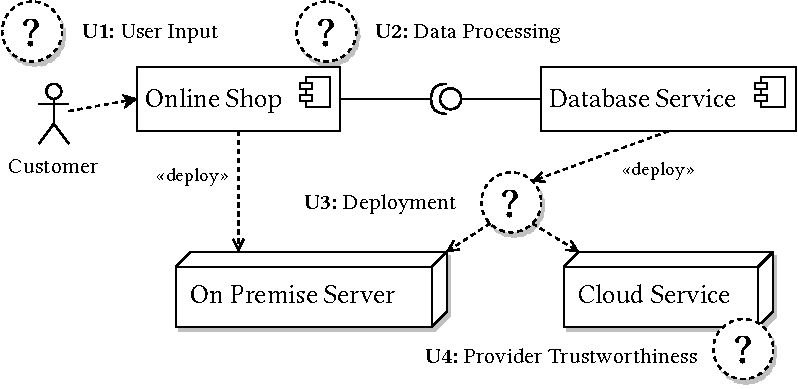
\includegraphics[width=0.9\textwidth]{figures/chapter3/onlineshop-architecture.pdf}
    \caption[Combined component and deployment diagram of the running example.]{Combined component and deployment diagram showing the software architecture of the online shop running example with annotated uncertainty sources depicted as circled question marks.}
    \label{fig:runningexample:architecture}
\end{figure}

The software architecture is depicted in \autoref{fig:runningexample:architecture}.
It consists of two components and two deployment locations. 
The \emph{Online Shop} component serves as the interface for customers while the \emph{Database Service} is used to persist information about customers, purchases, and the shop's inventory.
Both components are connected through an interface which is provided by the \emph{Database Service}.
The \emph{Online Shop} component is deployed on an \emph{On Premise Server} while the \emph{Database Service} can either be deployed locally on the same server or alternatively on a \emph{Cloud Service} for better scalability.

Customers interact directly with the \emph{Online Shop} component.
The running example comprises three usage scenarios.
First, customers input search details and request to view available items.
Second, they select an item to purchase and enter payment and shipping details.
In both scenarios, the input is processed in the \emph{Online Shop} component first.
Afterward, data is exchanged with the database, e.g., to query the inventory, or to store the purchase history.
The third usage scenario considers users that request static information like support contact addresses.
This information is provided directly by the \emph{Online Shop} component without any communication with the database.

We consider two types of data in the running example: The online shop's public information, and the user's private purchase details.
The former is publicly available and does not have to be protected---on the contrary, the online shop benefits from the public availability of this information.
The latter can be classified as personal or sensitive information for which confidentiality requirements apply.
Public availability of the customers' shopping and payment details would harm their privacy and might cause fraud or theft.
The European \acf{GDPR} demands that personal data of European citizens is only allowed to be stored and processed on European servers or on servers which ensure \enquote{an adequate level of protection} \cite[Art.~45]{council_of_european_union_regulation_2016}.
In the following, we assume that the online shop is operated in Europe, which implies that data processing on the \emph{On Premise Server} complies with this confidentiality requirement.
Depending on the cloud's server location and the trustworthiness of the provider, the storage on the \emph{Cloud Service} might violate this requirement.
Additional confidentiality requirements can include the user input, which has to be neither erroneous nor malicious, and also has to be validated and encrypted as part of the \emph{Online Shop} processing.

\begin{figure}
    \centering
    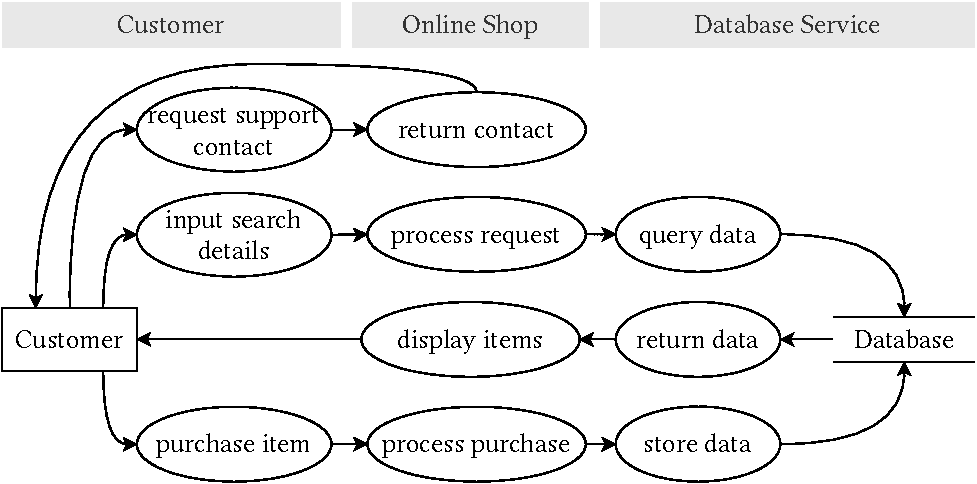
\includegraphics[width=0.9\textwidth]{figures/chapter3/onlineshop-dfd.pdf}
    \caption[Exemplary \acf*{DFD} of the running example.]{Exemplary \acf*{DFD} illustrating possible data flows through the online shop running example. The gray boxes indicate the user and components of the software architecture.}
    \label{fig:runningexample:dfd}
\end{figure}

We illustrate the behavior and data flows of the running example as \acf{DFD} in \autoref{fig:runningexample:dfd}.
In addition to the \ac{DFD} elements introduced in \autoref{sec:foundations:dfd}, we depict the users and components using gray boxes \cite{seifermann_architectural_2022}.
The upper half of the diagram represents the flow of query requests from the user via the online shop to the database and the response containing available items from the database to the user.
Additionally, it shows the request for support information.
In our simplified example, both data flows do not contain sensitive information.
Thus, no confidentiality requirements apply.
In the lower half, the customer purchases an item.
The purchase is processed on the online shop and then stored in the database.
This data flow is subject to confidentiality requirements.





\section{Exemplary Uncertainty Sources}%
\label{sec:runningexample:uncertainty}

As described previously in \autoref{sec:foundations:uncertainty}, uncertainty sources can exist within the software system and its environment \cite{acosta_uncertainty_2022}.
In \autoref{fig:runningexample:architecture} and in the following, we represent uncertainty sources in diagrams as circled question marks.
We introduce four exemplary yet common sources of uncertainty to our running example:

\begin{enumerate}[label=\textbf{U\arabic*}]
    \item The users' input is a source of uncertainty. Although certain behavior regarding entered information can be expected already at design time, it cannot be guaranteed. % https://arc3n.abunai.dev/uncertainty/52 (Connector)
    \item The data processing is still uncertain. This can be the case due to an open design decision or due to the black box nature of a third-party off-the-shelf component. % https://arc3n.abunai.dev/uncertainty/35 (Behavior)
    \item The component deployment is an uncertainty source. This can be caused by missing design decisions or dynamic reconfiguration at runtime, e.g., due to load balancing. % https://arc3n.abunai.dev/uncertainty/59 (Component)
    \item The trustworthiness of a resource provider, which is used as a deployment location for a component or service, is uncertain and can only be assured, e.g., with policies. % https://arc3n.abunai.dev/uncertainty/48 (External)
\end{enumerate}

We annotate the first Uncertainty \U{1} to the customer using the online shop.
Humans are a common uncertainty source within the literature, often referred to as \emph{human in the loop} \cite{perez-palacin_uncertainties_2014,ramirez_taxonomy_2012}.
Although the user input is uncertain, we can assume different input classes, e.g., valid input as expected, erroneous input due to human failure, or malicious input.

The second uncertainty source \U{2} considering the data processing is annotated to the \emph{Online Shop} component and its connection to the \emph{Database Service}.
This could be uncertain due to the black-box principle of software components \cite{reussner_modeling_2016} or due to a yet-to-be-defined design decision \cite{lytra_supporting_2013}.
In our example, this could affect confidentiality if we do not know whether all requests to the \emph{Database Service} are encrypted before sending.
Additionally, input validation could be part of the processing, which analyzes the users' input to counter Uncertainty \U{1}.
Also, combinations of input validation and encryption are imaginable.

The third uncertainty source \U{3} affects the deployment of the \emph{Database Service} and is annotated on the associated arrow.
Deployment decisions could be still uncertain at design time \cite{mcconnell_software_1998}, or depend on the runtime situation, e.g., in the context of \acfp{SAS} \cite{weyns_introduction_2020}.
In \autoref{fig:runningexample:architecture}, we show two possible deployment locations, with the \emph{Database Service} being either deployed on-premise or in the cloud.

The fourth uncertainty source \U{4} is annotated to the \emph{Cloud Service} and questions the providers' trustworthiness.
Providers could void confidentiality either intentionally, e.g., by misusing data \cite{costante_privacy-aware_2013}, or unintentionally, e.g., due to the lack of proper security requirements and appropriate measures \cite{firesmith_specifying_2004}.
To that end, we can only assume the trustworthiness and categorize whether providers are trustworthy enough or not.

Other and additional uncertainty sources are also possible within the running example, see \arcen.
We selected these uncertainties as they demonstrate different locations, types, and origins, while still keeping the running example simple and easy to understand.





\section{Summary and Outlook}%
\label{sec:runningexample:summary}

In this chapter, we introduced a running example that will be used throughout this thesis.
Already a software system of the size of our running example shows the challenge of dealing with multiple uncertainty sources.
Uncertainty sources and impact locations arise at different points within the software system and its environment, which might cause complex interrelations and interactions \cite{camara_uncertainty_2024} regarding confidentiality.
Especially in larger software systems, analyzing them manually is not expedient.
Thus, we need proper modeling, analysis, and mitigation strategies to ensure confidentiality.

Note, that the \ac{DFD} shown in \autoref{fig:runningexample:dfd} also depends on the outcome of the uncertainty sources \U{1} -- \U{4}.
Uncertainty \U{1} could alter the customer process \emph{input search details}, or Uncertainty \U{3} could affect the structure of the \ac{DFD}.
Additionally, the concrete form of the \ac{DFD} depends on the level of abstraction \cite{demarco_structure_1979}.
Building on previous advances in uncertainty representation \cite{garlan_software_2010,troya_uncertainty_2021}, we find that:

\finding{Even small software systems like our running example can have many corresponding data flow diagrams under uncertainty. 
Uncertainty hinders precise modeling and analysis when not included properly within the model.}

The presentation of the running example was based on \acp{DFD} and uncertainty which both have been introduced in \readingpath{ch:foundations}.
Next, we use the running example to give an overview of all contributions in \readingpath{ch:overview}.
We modeled the software architecture of the running example based on the \acf{PCM}.
The model files can be found in our data set \cite{dataset}.
An overview and first impression is given in \autoref{sec:appendix:runningexample}.





\section{In Simpler Words}%
\label{sec:runningexample:simple}

A simple running example makes it easier to understand complex ideas.
We introduce the running example of an online shop known from everyday life.
Online shops deal with customer data and are thus required to protect that data and keep it confidential.
Additionally, we presented different sources of uncertainty in our example.
Examples are the behavior of customers or the trustworthiness of cloud service providers.
Even in this simple example, we can see how this uncertainty harms confidentiality.
For example, if we are unsure whether providers behave maliciously, customers' stored data could be threatened.
One approach to face the challenge of analyzing confidentiality under uncertainty will be presented in the remainder of this thesis.

\part{Contributions}
\chapter{Overview}%
\label{ch:overview}%


In this chapter, we give an overview of the contributions of this dissertation.
This shall serve both as an introduction and as a high-level summary of the detailed explanations in the following chapters.
All contributions can be located in the research area of design time analysis and architecture-based quality prediction \cite{reussner_modeling_2016}.
Here, common benefits are simplifying the work of software architects and enhancing existing analysis approaches, e.g., regarding their applicability, scalability, accuracy, or usability \cite{konersmann_evaluation_2022}.

The central research concern of this thesis is confidentiality analysis under uncertainty by using architectural modeling \cite{hahner_dealing_2021}.
We divide the contributions of this thesis into three parts:
First, the identification and classification of uncertainty regarding confidentiality.
Second, the uncertainty impact analysis by propagating uncertainty within architectural models and data flow diagrams.
Third, the architecture-based confidentiality analysis under uncertainty.
Each of these contributions can be used independently and enhances the state of the art in its area.
However, they can also be combined to form a comprehensive end-to-end approach which is an aspired goal in the community \cite{weyns_towards_2023,hezavehi_uncertainty_2021}.

In the following, we describe the general procedure for uncertainty-aware analyses and how our contributions are positioned within it.
We briefly introduce these contributions afterward.
Last, we give an overview of the tool support that has been developed to complement the research.

\ownpublications{
\fancycite{hahner_dealing_2021}, 
\fancycite{hahner_architectural_2021}, 
\fancycite{acosta_uncertainty_2022}, 
\fancycite{hahner_model-based_2023}, 
\fancycite{hahner_classification_2023},
\fancycite{camara_uncertainty_2024},
\fancycite{hahner_arcn_2024}
}





\section{Procedure for Uncertainty-Aware Analyses}%
\label{sec:overview:procedure}

Incorporating uncertainty in the analysis of software systems---thus achieving uncertainty awareness---has been discussed within the literature \cite{garlan_software_2010,sobhy_evaluation_2021,troya_uncertainty_2021}.
\textcite{garlan_software_2010} proposed to include uncertainty as \enquote{first-class concern in the design, implementation, and deployment} of software systems.
\textcite{hezavehi_uncertainty_2021} conducted a community survey and proposed a reference process for uncertainty management.
They include phases like identification, modeling, impact analysis, and assessment.
However, their process aims at \acfp{SAS} that include run time strategies that are beyond the scope of this thesis.
Regarding model-based analyses at design time \cite{acosta_uncertainty_2022}, we consider four central activities: 

\begin{enumerate}
    \item \textbf{Identification and awareness}: 
    To include uncertainty sources in the analysis, they must be known first.
    Thus, raising awareness to recognize the presence of uncertainty in a system is the necessary first step.

    \item \textbf{Classification}: 
    To better understand the type of uncertainty sources and their properties, they can be classified.
    To that end, classifications and taxonomies provide the foundations for the documentation and the discussion of identified uncertainty.

    \item \textbf{Propagation}: To assess the impact of identified and classified uncertainty sources, they can be propagated through the architectural model.
    Estimating the potential impact early helps in making more precise statements and decisions.

    \item \textbf{Analysis}: To apply appropriate mitigation strategies, the effect of uncertainty on the software system's quality has to be analyzed.
    In our case, this means identifying confidentiality violations due to the identified, classified, and propagated uncertainty.
\end{enumerate}

\begin{figure}
    \centering
    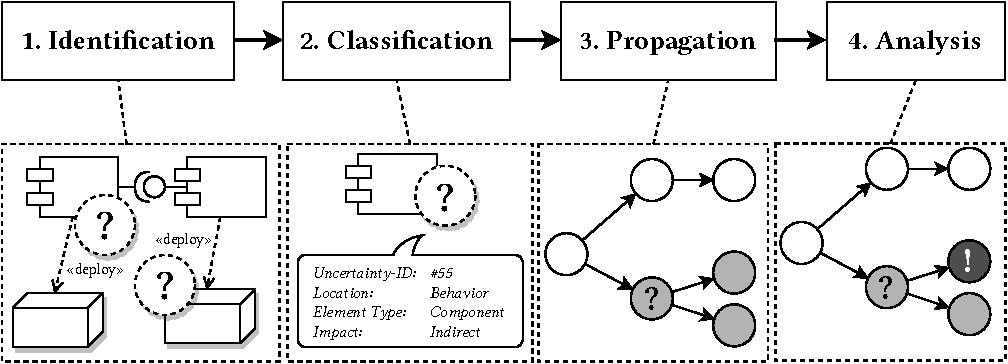
\includegraphics[width=\textwidth]{figures/chapter4/overview-informal.pdf}
    \caption{Informal overview of the central activities of uncertainty-aware analyses}
    \label{fig:overview:informal}
\end{figure}

\autoref{fig:overview:informal} illustrates these four activities in an informal diagram.
\emph{First}, uncertainty sources have to be identified, e.g., within the software system or its environment.
In \autoref{fig:overview:informal}, we annotate these uncertainty sources in the architectural model similar to the running example presented in \autoref{ch:runningexample}.
In the \emph{second} activity, these uncertainty sources have to be described according to an appropriate classification \cite{hahner_classification_2023}.
This does not only help in the understanding of the underlying problem but also enables an uniform handling in the later activities.
The \emph{third} activity is the propagation of uncertainty sources to estimate their potential impact.
Here, software architects develop an understanding of which parts of the software systems could be affected and which parts can be safely ignored.
The \emph{fourth} activity is the confidentiality analysis under uncertainty.
This activity yields confidentiality violations in those parts of the software system that have been impacted by uncertainty.

\finding{Literature proposed processes for uncertainty management.
Common steps are the identification, classification, propagation, and analysis of uncertainty.
By applying these activities to confidentiality analysis, we can provide a comprehensive approach to identify confidentiality violations under uncertainty.}

A high-level description like the informal overview introduced in \autoref{fig:overview:informal} serves as an overview or introduction.
However, due to the high abstraction, two important details are left out.
\emph{First}, the procedure does not need to be linear.
Sometimes, not all activities are required, e.g., because a critical subsystem has to be always analyzed despite the results of the propagation.
Additionally, some activities or the procedure might be repeated, either because of the understanding of the uncertainty or because the system evolves \cite{weyns_towards_2023}.
Especially with regard to uncertainty and \acp{SAS}, approaches tend to be iterative and incremental, as in continuous architecture evaluation \cite{sobhy_evaluation_2021}, or in the \acf{MAPEK} loop \cite{kephart_vision_2003,weyns_patterns_2013}.
\emph{Second}, the informal overview lacks role descriptions.
Specifying expertise and required knowledge helps in understanding the application of analysis procedures.

\begin{figure}
    \centering
    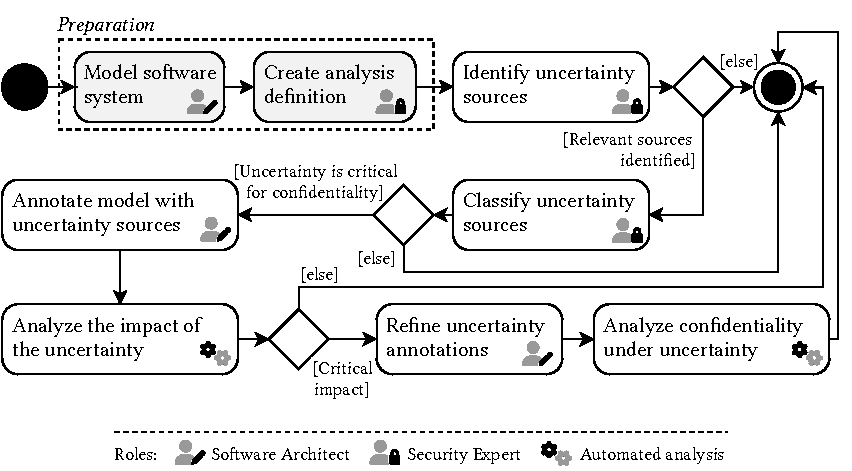
\includegraphics[width=\textwidth]{figures/chapter4/overview-procedure.pdf}
    \caption{Proposed analysis procedure showing the modeling and analysis activities and assigned roles.}
    \label{fig:overview:procedure}
\end{figure}

To address these shortcomings, we provide a more detailed procedure with \autoref{fig:overview:procedure}.
We reuse the roles proposed for architectural confidentiality analysis \cite{seifermann_architectural_2022}, i.e., \emph{software architect} and \emph{security expert}.
Note, that we do not introduce a role for \emph{uncertainty experts}.
With appropriate means like tool-supported identification, classification, and analysis approaches, only minimal additional knowledge shall be required.
Thus, we do require expert knowledge of uncertainty classification or uncertainty sources in general.

The procedure starts with the preparation phase which comprises modeling the software system \cite{seifermann_data-driven_2019,seifermann_identifying_2021} and creating the analysis definition \cite{hahner_modeling_2021}.
These steps originate from architectural data flow analysis \cite{seifermann_architectural_2022}.
An architectural model has to be defined by a software architect using an \acf{ADL} like the \acf{PCM} or \acfp{DFD}.
Afterward, confidentiality requirements serve as input for the security expert to create the confidentiality analysis definition.
This enables identifying confidentiality violations without considering uncertainty.

First, uncertainty sources have to be identified by the security expert.
Although we do not require expert knowledge of uncertainty, security expertise helps estimate the potential impact on confidentiality.
Uncertainty sources can be identified in discussions, architecture reviews, or using checklists, guidelines, or catalogs \cite{hahner_arcn_2024}. 
If no relevant sources have been identified, the procedure ends until new knowledge about uncertainty is gained.
This step represents the first activity of identification and awareness. 

In the next step, the identified uncertainty sources are classified according to an appropriate classification \cite{hahner_classification_2023}.
This step is performed by the security expert with the help of existing catalogs that bootstrap the classification.
If only uncertainty sources have been identified that clearly have no impact on confidentiality, the procedure ends.
This step represents the second activity.
Based on the result of the classification, the uncertainty sources are annotated to the architectural model.
This does not require security expertise but knowledge of the \ac{ADL} in use and is thus driven by the software architect.

Afterward, the uncertainty impact analysis propagates the uncertainty source within the software system and calculates the potential impact \cite{hahner_architecture-based_2023}.
This step represents the third activity and is fully automated and thus requires neither knowledge about security nor software architecture.
If no relevant uncertainty impact is identified, e.g., because only non-critical parts of a software system are affected, the procedure ends.
Otherwise, the confidentiality under uncertainty has to be analyzed which is the fourth activity.
This includes a more detailed specification of the uncertainty sources for a precise analysis result.
While the refinement of the information about the uncertainty is conducted by the software architect, the analysis is fully automated.
Afterward, the procedure ends.

Note that the end of the procedure does not imply the end of the design and analysis process.
If the knowledge about uncertainty or the software systems changes, the procedure can be restarted.
Additionally, all artefacts like the modeled software architecture, the analysis definition, collected uncertainty sources and their classification and annotation can be reused.
Thus, we consider this procedure to be iterative.
As stated previously, we do not require expert knowledge about uncertainty.
The classification and the automated analyses, i.e., the uncertainty impact analysis and the uncertainty-aware confidentiality analysis encapsulate the required knowledge \cite{hahner_model-based_2023}.
The procedure has to be incremental as the existence of uncertainty is inherent to software systems.
It can never be assured to be aware of all uncertainty sources, as \emph{unknown unknowns} \cite{perez-palacin_uncertainties_2014} might exist.
In this way, uncertainty is similar to bugs in software systems, where testing can only be used to show the \enquote{presence of bugs, but never to show their absence} \cite{dijkstra_notes_1970}.
Additionally, the procedure requires exit points after each activity when more knowledge is gained about the impact of uncertainty on the software system's confidentiality.

\finding{Due to the nature of uncertainty, it is impossible to ensure its absence.
However, not every uncertainty source causes confidentiality violations.
This depends on many aspects like the uncertainty itself, confidentiality requirements, security measures, or the software's architecture.
A procedure for uncertainty-aware confidentiality analysis has to be iterative and incremental.}





\section{Overview of the Contributions}%
\label{sec:overview:contributions}

In the following, we introduce the central contributions of this thesis and relate them to the procedure presented hereabove.
We divide the contributions into three main parts:

\begin{enumerate}[label=\textbf{C\arabic*}]
    \item \textbf{Identification and classification}: Recognizing and understanding the types of uncertainty and their relation to confidentiality from an architectural point of view.
    \item \textbf{Uncertainty impact analysis}: Propagating uncertainty using architectural models and \acp{DFD} to predict the uncertainty impact on the system's confidentiality.
    \item \textbf{Uncertainty-aware confidentiality analysis}: Extending architecture-based confidentiality analysis to consider uncertainty as a first-class concern in both modeling and analysis to identify confidentiality violations under uncertainty.
\end{enumerate}

First, with Contribution \C{1}, we aim to support software architects in identifying and classifying relevant uncertainty sources with a potential impact on confidentiality.
This is an elemental first step, as awareness about uncertainty sources and their properties is key in documentation, modeling, discussion, and analysis \cite{garlan_unknown_2021}.
This combines the activities of identification and classification in one contribution, as both are interdependent and support each other.
We contribute a classification of software-architectural uncertainty \cite{hahner_classification_2023} and support the collaborative identification of uncertainty sources \cite{hahner_arcn_2024}.
During this research, we also examine \acfp{CPS} as a relevant type of uncertainty-afflicted software systems \cite{acosta_uncertainty_2022}.
Our findings answer \RQ{1}, which is related to the identification and description of uncertainty with regard to confidentiality.

Our second Contribution \C{2} addresses the impact analysis of uncertainty, which supports the early prediction and assessment of the uncertainty impact.
Similar to change impact analysis \cite{rostami_architecture-based_2015,rostami_architecture-based_2017}, we propagate uncertainty through the software architecture.
Besides the theoretical foundations of modeling and propagating uncertainty in architectural models and \acp{DFD}, this contribution also includes a fully automated analysis \cite{hahner_architecture-based_2023}.
Based on our concept of uncertainty propagation in \acp{DFD}, additional research led to the formulation of \acp{UFD} \cite{camara_uncertainty_2024}.
They support software architects in understanding and analyzing uncertainty interactions \cite{camara_addressing_2022}.
In sum, these findings provide an answer to \RQ{2}, which relates to architectural uncertainty propagation and impact analysis.

In our third Contribution \C{3}, we develop confidentiality analysis approaches that respect uncertainty.
To that end, we extend an existing architecture-based confidentiality analysis which utilizes \acp{DFD} \cite{seifermann_architectural_2022,seifermann_detecting_2022}.
We provide approaches for different types of uncertainty, e.g., environmental uncertainty \cite{boltz_handling_2022}, or structural uncertainty \cite{walter_architectural_2022}.
By defining an analysis framework for architectural data flow analysis, we also provide the baseline for more comprehensive approaches \cite{boltz_extensible_2024}.
We use this framework to research the expressiveness, accuracy, and scalability of data flow-based confidentiality analysis under uncertainty \cite{hahner_model-based_2023}.
These approaches address \RQ{3}, which asks how to consider uncertainty in architectural confidentiality analysis. 





\section{Tool Support}%
\label{sec:overview:toolsupport}

In addition to answering the research questions of this thesis, we provide comprehensive tool support.
For each contribution, we realized tooling to demonstrate the applicability of the concepts.
The prototypical implementation is not only used in the evaluation but also shall support further research \cite{boltz_extensible_2024}.
A recent \acf{SLR} found a lack of replication packages in software architecture research \cite{konersmann_evaluation_2022}.
To address this, all tool support is open source, publicly available and also part of this thesis' data set \cite{dataset}.

Automated analyses support software architects because they encapsulate expert knowledge, e.g., annotation and propagation rules \cite{hahner_classification_2023}.
Especially in large software systems or systems of systems, manual analysis is also not feasible and error-prone \cite{seifermann_data-driven_2019}.
In our iterative procedure, it cannot be assumed that software architects manually evaluate hundreds of \ac{DFD} nodes \cite{hahner_classification_2023} without mistakes.
Additionally, after each change to the annotated uncertainty sources or the software system, the manual work would have to start all over again.
Thus, it is important to ensure that the developed concepts can be automated to a high degree without manual effort required from software architects.
Similar to the division into three contributions, we provide three tooling artifacts.
We introduce and shortly summarize their functionality in the following%
\footnote{At the time of writing---and hopefully a long time to come---the most up-to-date version of all tool support is online available here: \url{https://abunai.dev/}. Once the link is broken, please refer to the data set \cite{dataset}.}.

\arcen stands for rese\uff{arc}h \uff{arc}hive for Software-\uff{arc}hitectural u\uff{n}certainty.
This is a web-based interactive catalog of uncertainty sources that can affect confidentiality \cite{hahner_arcn_2024}.
It simplifies the identification by connecting a classification \cite{hahner_classification_2023} to a catalog approach.
All data is publicly available, extensible by other researchers, and can be integrated into existing analyses.
This catalog of uncertainty sources supports Contribution \C{1}.

\uia means \uff{u}ncertainty \uff{i}mpact \uff{a}nalysis and is a tool for propagating uncertainty sources within architectural models and \acp{DFD}.
It extends the data flow analysis framework \cite{boltz_extensible_2024}.
The tool support is realized as an Eclipse plugin and can be integrated into the existing Palladio tooling \cite{reussner_modeling_2016}.
The analysis yields an impact set for uncertainty sources which can be annotated to the software architecture.
Besides the annotation, no additional effort is required for existing \ac{PCM} models as the propagation is fully automated.
See \autoref{sec:appendix:impactset} for an exemplary impact analysis result.
This supports our second Contribution \C{2}.

\abunai is short for \uff{a}rchitecture-\uff{b}ased and \uff{un}certainty-\uff{a}ware confidentiality analys\uff{i}s\footnote{Furthermore, the Japanese word \emph{abunai} translates to dangerous, risky, or uncertain. How fitting!}.
Similarly to the uncertainty impact analysis, this tooling is realized as an Eclipse plugin and extends the data flow analysis framework \cite{boltz_extensible_2024} within the Palladio approach \cite{reussner_modeling_2016}.
This analysis enables software architects to refine the uncertainty annotations by providing possible scenarios \cite{hahner_model-based_2023}.
Afterward, the automated analysis considers the uncertainty impact in the data flow analysis and yields confidentiality violations with respect to uncertainty.
See \autoref{sec:appendix:runningexample} and \autoref{sec:appendix:confidentiality} for exemplary analysis inputs and analysis results.
This is one of the analysis approaches that support Contribution \C{3}.





\section{Illustration using the Running Example}%
\label{sec:overview:illustration}

We demonstrate the procedure, the contributions, and the tool support briefly using the running example introduced in \autoref{ch:runningexample}.
We assume a team of software architects and security experts that already modeled the software system using \ac{PCM} and created the analysis definition to analyze the system's confidentiality.
See the preparation phase in \autoref{sec:overview:procedure} for more details.

First, relevant uncertainty sources have to be identified by security experts.
As part of our first Contribution \C{1}, the tool support \arcen provides a catalog of uncertainty sources that serve as a starting point.
The catalog also contains all uncertainty sources which have been annotated to the running example, e.g., the user input (\U{1}), or the provider's trustworthiness (\U{4}).
As the uncertainty sources in this catalog already are classified, the subsequent step of uncertainty classification is simplified or can be skipped.
All of the contained sources are relevant regarding confidentiality.
The software architect annotates the uncertainty sources within the architectural model in the running example.
For example, the user input uncertainty (\U{1}) is annotated to the \emph{Customer}, and the data processing uncertainty (\U{2}) is annotated to the \emph{Online Shop} component.
In \autoref{fig:runningexample:architecture}, we illustrate this annotation using circled question marks.

Using the architectural models and the annotations as input, the impact analysis calculates the potential impact on confidentiality.
This is part of our second Contribution \C{2}, and fully automated with \uia.
In the running example, the impact set of all uncertainty sources contains the \emph{Database Service} component.
As the database stores confidential data, we interpret this impact as being critical continue with the step of uncertainty source refinement.
The precise modeling of uncertainty sources and scenarios and the analysis are part of our third Contribution \C{3}.
In the running example, the software architects describe all relevant scenarios, e.g., the possible deployment locations of the \emph{On Premise Server} or the \emph{Cloud Service}.
Afterward, the automated analysis \abunai yields confidentiality violations due to single or multiple uncertainty scenarios.
In our running example, the lack of proper data processing (\U{2}) and the deployment in the cloud (\U{3}) without proper security measures violate confidentiality.
After addressing these issues, the procedure can be repeated.
This also happens whenever the software system changes, e.g., due to the introduction of a new encryption component, or the knowledge about the uncertainty changes, e.g., because the scenario of the lack of any data processing can be excluded.





\section{Summary and Outlook}%
\label{sec:overview:summary}

In this chapter, we discussed the procedure of uncertainty-aware analysis and summarized the contributions of this thesis.
First, we investigated multiple proposals for required activities in uncertainty-aware analysis.
We combined them to propose a procedure for architecture-based confidentiality analysis under uncertainty.
This procedure contains the central activities of identification, classification, propagation, and analysis.
Besides these activities, our proposed procedure also contains modeling activities carried out by software architects and security experts.
The analyses are fully automated and thus shall not require additional knowledge about uncertainty.
The procedure is both iterative and incremental to react to changes in the system, its environment, and its uncertainty sources.
Put simply, uncertainty is uncertain, and we have to deal with it.

Afterward, we gave an overview of the central contributions of this thesis.
They cover the aforementioned activities of identification and classification with Contribution \C{1}, the propagation and uncertainty impact analysis with Contribution \C{2}, and the uncertainty-aware confidentiality analysis with Contribution \C{3}.
All contributions are tool-supported with three research artifacts: \arcen collects and explains uncertainty sources and their classification, \uia automatically propagates uncertainty in an architectural model to calculate the potential impact, and \abunai provides uncertainty-aware confidentiality analysis based on architectural modeling and \acp{DFD}.
Last, we illustrated the tool-supported contributions and their interrelationships using the running example.
The application of our prototypical tooling is also shown in \autoref{sec:appendix:runningexample}, \autoref{sec:appendix:impactset}, and \autoref{sec:appendix:confidentiality}.

Throughout this chapter, we stressed the lack of an explicit role for uncertainty experts in the proposed procedure.
Ideally, automated analyses and other artifacts should encapsulate the required knowledge about uncertainty.
We will return to this idea in the following chapters and explain the consequences in more detail.
The illustration in this chapter was based on \readingpath{ch:runningexample}.
In the following three chapters, we present the contributions in detail.
In \readingpath{ch:classification}, we show the first Contribution \C{1}, in \readingpath{ch:impactanalysis}, we introduce the second Contribution \C{2}, and in \readingpath{ch:confidentialityanalysis}, we discuss the third Contribution \C{3}.





\section{In Simpler Words}%
\label{sec:overview:simple}

This chapter gives an overview that helps to better understand the relation of the individual contributions of this thesis.
Our central research concern is analyzing confidentiality under uncertainty.
Uncertainty can threaten the confidentiality of sensitive user data like names or addresses.
An example is the uncertainty about the encryption of this data.
If we cannot guarantee the correct encryption, we cannot guarantee confidentiality.

We propose four activities which help to act upon such uncertainty.
First, the uncertainty sources have to be identified and described.
We developed tools that contain catalogs and descriptions of uncertainty sources.
This minimizes the effort and expertise requirements of software architects and security experts.
Afterward, we assess the impact of uncertainty on confidentiality using an automated analysis.
For example, the lack of encryption could impact confidentiality.
Our contributions help to identify that this uncertainty exists and how great its impact is.
If the impact is relevant, our automated analysis helps to find confidentiality violations that can be caused by this uncertainty.
\chapter{Identification and Classification of Uncertainty Regarding Confidentiality}%
\label{ch:classification}%
 

In this chapter, we present the first Contribution \C{1}.
This contribution covers the first two activities shown in \autoref{sec:overview:procedure}, i.e., the identification and classification of uncertainty.
We focus on confidentiality as a central quality property for this thesis.

As introduced in \autoref{ch:introduction}, confidentiality demands that \enquote{information is not made available or disclosed to unauthorized individuals, entities, or processes} \cite{international_organization_for_standardization_isoiec_2018}.
With the growing size and connections of today's software systems, ensuring confidentiality becomes a major challenge. 
We describe in \autoref{ch:overview} that we use design-time confidentiality analysis \cite{seifermann_detecting_2022,tuma_flaws_2019} to identify flaws early and to avoid costly repairs of running systems \cite{boehm_software_2001}.
Here, data flow-oriented analyses became common because \enquote{problems tend to follow the data flow, not the control flow} \cite{shostack_threat_2014}.
However, especially in early development and in complex systems of systems, the software architecture is subject to uncertainty.
This does not only affect decision making---also known as the \emph{cone of uncertainty} \cite{mcconnell_software_1998}---but even blurs which decisions should be prioritized.
When not managed properly, the lack of awareness of uncertainty can void a system's confidentiality.
Also, the \ac{OWASP} Top 10 \cite{OWASPTop10} lists issues like \emph{insecure design} as top security risks.
Thus, we have to actively address the phenomenon of uncertainty and its impact on the confidentiality analysis results.

Managing uncertainty includes activities like the identification and classification \cite{acosta_uncertainty_2022,weyns_introduction_2020,hezavehi_uncertainty_2021}.
Here, multiple taxonomies were defined to better understand the nature of uncertainty \cite{perez-palacin_uncertainties_2014,ramirez_taxonomy_2012,walker_defining_2003}.
However, they mostly originate from the domain of \acfp{SAS} and do not focus on confidentiality.
The consequences are a lack of applicability and an increase in ambiguity.
The relation of software architecture, confidentiality and uncertainty remains unclear \cite{hahner_dealing_2021}.
And while \enquote{there is growing consensus on the importance of uncertainty} \cite{hezavehi_uncertainty_2021}, much is yet unknown regarding the impact of uncertainty on software systems \cite{garlan_software_2010}.
Hezavehi et al. \cite{hezavehi_uncertainty_2021} conducted a survey on uncertainty.
They find a \enquote{lack of systematic approaches for managing uncertainty} \cite{hezavehi_uncertainty_2021} and that uncertainty should already be addressed at design time.
This statement is supported by the work of Troya et al. \cite{troya_uncertainty_2021}.
They conducted a \acf{SLR} and analyzed 123 papers.
They state that \enquote{software models are still falling short of explicitly representing uncertainty} \cite{troya_uncertainty_2021} and that
software engineers require more help \enquote{to identify the types of uncertainty that can affect their application domains} \cite{troya_uncertainty_2021}.

Uncertainty can arise within software systems, e.g., design choices, or reconfiguration at runtime, and their environment, e.g., sensor data, or humans in the loop \cite{acosta_uncertainty_2022,perez-palacin_uncertainties_2014}.
To enhance existing confidentiality analysis approaches, software architects require already known uncertainty sources, which are also called \emph{known unknowns} or first-order uncertainty \cite{perez-palacin_uncertainties_2014}, e.g. known variation of sensors or user behavior.
Second-order uncertainty, also called \emph{unknown unknowns}, cannot be analyzed due to the lack of knowledge about its sources, e.g., due to unforeseen environmental conditions, which limits the development of mitigation strategies \cite{weyns_towards_2023}.
This \acf{UAP} impedes the comprehensive analysis of software systems which poses security threats that could have been resolved at design time.
However, it is a highly subjective phenomenon, as it only depends on the knowledge or awareness of the software architect conducting the analysis. 
Put simply, one cannot analyze what one does not know.

The \ac{UAP} and the related need for collecting uncertainties are supported in the literature.
Recent surveys and research agendas highlight this problem of dealing with unanticipated change \cite{weyns_introduction_2020}, the need to share knowledge of uncertainty \cite{hezavehi_uncertainty_2021}, and the development of \enquote{reusable methods to assess and manage uncertainties} \cite{weyns_towards_2023}.
A class between known and unknown uncertainty was proposed, as not every change is completely unanticipated and can be addressed by flexible designs using intentional over-engineering or meta-adaptation \cite{garlan_unknown_2021}.
To address this, classification approaches alone are not sufficient but require additions like collections and surveys \cite{ramirez_taxonomy_2012,troya_uncertainty_2021}, or expert knowledge \cite{lytra_supporting_2013,esfahani_guidearch_2013}.
Classifications only describe properties of uncertainty which does not resolve the awareness problem, publication-based collections are hard to extend dynamically and are thus prone to become outdated and incomplete, and relying on experts is not expedient.
Developing a joined approach of identification and classification is a step towards end-to-end approaches that promise a higher impact than incrementally enhancing existing analyses \cite{weyns_towards_2023}.

In sum, we aim to address both the identification and classification problem to include uncertainty in confidentiality analysis based on \acfp{DFD}.
This breaks the limitation of previous approaches that were only able to analyze confidentiality with perfect knowledge, i.e., by excluding uncertainty about software systems and their data \cite{seifermann_architectural_2022}.
We summarized this research concern in the first research question:

\RQone

The remainder of this chapter is structured as follows:
First, we summarize the problem statement.
We revisit the relation of uncertainty, confidentiality, and software architecture.
We investigate existing uncertainty classifications and their appropriateness to addressing confidentiality.
Then, we define a new classification of uncertainty regarding confidentiality and discuss, based on this classification, how to represent uncertainty in data flow diagrams.
Afterward, we build on the classification to present an uncertainty catalog approach that helps in the identification of uncertainty and addresses the \ac{UAP}.
We close the chapter with known assumptions and limitations, and also a summary and an outlook.

\ownpublications{
\fancycite{hahner_dealing_2021},
\fancycite{hahner_architectural_2021},
\fancycite{acosta_uncertainty_2022},
\fancycite{hahner_classification_2023},
\fancycite{hahner_arcn_2024}
}





\section{Problem Statement}%
\label{sec:classification:problem}

We summarize the problems \textbf{P1} -- \textbf{P5} addressed by Contribution \C{1}.
Finding solutions to these problems helps to provide a comprehensive answer to \RQ{1}.

\paragraph{P1: Knowledge about the relation of uncertainty and confidentiality}\label{p:1:1}
We need to better understand the role of uncertainty and its relation to confidentiality in software architecture.
This includes considering uncertainty at design time and runtime and also relating uncertainty to \acfp{ADD}, which is related to architectural decision-making under uncertainty \cite{lytra_supporting_2013}.
We see this as a precondition to defining precise classifications of uncertainty regarding confidentiality \cite{hahner_dealing_2021}.
The solution to this problem is considered to be non-trivial due to the variety of uncertainty.

\paragraph{P2: Classification of uncertainty tailored to confidentiality}\label{p:1:2}
We require classifications tailored to confidentiality and software architecture.
There exist classifications from other domains \cite{perez-palacin_uncertainties_2014,ramirez_taxonomy_2012,walker_defining_2003}, but they fall short in representing the impact of uncertainty on confidentiality.
Additionally, they do not relate the classified uncertainty to software architecture and \acp{ADD}.
Here, a classification scheme to aid software architects in understanding the impact of uncertainty on confidentiality. 
This shall raise awareness of properties of uncertainty and their relevance for choosing appropriate \acp{ADD} and mitigation strategies. 
We intentionally speak of a classification rather than a taxonomy because we focus on a subset of uncertainty, i.e., known uncertainty on architectural abstraction.

\paragraph{P3: Representation of uncertainty as first-class concern in \acp{DFD}}\label{p:1:3}
\textcite{garlan_software_2010} raised the need to represent uncertainty as a first-class concern in the design of software systems.
This applies to \acp{ADL} as well as to \acp{DFD}.
Whether in tool-supported analysis or in discussions between software architects, uncertainty must be represented appropriately to be taken into account.
This includes defining a notation for uncertainty impact in \acp{DFD} that works for all uncertainty types of the classification.
Only limited work towards considering uncertainty in \acp{DFD} exists \cite{durugbo_data_2010}, which only considers selected uncertainty types.

\paragraph{P4: Expert knowledge required to understand uncertainty sources}\label{p:1:4}
Due to space limitations in publications, previous approaches only explain classifications briefly without comprehensive data sets \cite{ramirez_taxonomy_2012}.
We stress the importance of explainability \cite{bersani_conceptual_2023}, e.g., using examples, interactive visualizations, and context information from the underlying classification.
Additionally, classifications provide dimensions or categories to describe uncertainties but often fall short in relating multiple uncertainty types which impairs usability \cite{hahner_classification_2023}.
It should be possible to filter, search, and navigate between uncertainties, which requires defined relations between them.
This is especially relevant as uncertainty sources are rarely independent and interactions can occur \cite{camara_uncertainty_2024}.
We do not require an \emph{uncertainty expert} role in our procedure, see \autoref{sec:overview:procedure}.
Therefore, our contributions to the identification and classification must be understandable without extensive training.

\paragraph{P5: Extensible uncertainty source catalogs to support the identification}\label{p:1:5}
The \acf{UAP} states that we need awareness of uncertainty sources to consider them in the uncertainty mitigation process.
One approach to this problem is a collection of uncertainty sources, building on the solutions to the aforementioned problems.
However, publication-based collections are hard to reuse and extend \cite{ramirez_taxonomy_2012} and thus prone to become outdated and incomplete.
Knowledge can be scattered between researchers or organizations which complicates collaboration \cite{sterz_intelligente_2022}.
Additionally, research artifacts often are unavailable \cite{konersmann_evaluation_2022} or partially broken \cite{gerdes_decision_2015,colesky_system_2018}.
To address this, an open-source and publicly available catalog is required, which shall be easy to discuss and extend by researchers and practitioners. 
To enable the seamless integration into uncertainty-aware analyses and to enable end-to-end approaches \cite{weyns_towards_2023}, it shall be possible to transform the catalog into a machine-readable format like \acf{JSON} or \ac{XML}.
Related collections of architectural knowledge \cite{gerdes_decision_2015}, or privacy patterns \cite{colesky_system_2018} have shortcomings regarding usability, extensibility, and longevity of the contained information.





\section[The Relation of Uncertainty, Confidentiality, and Software Architecture]{Understanding the Relation of Uncertainty, Confidentiality, and Software Architecture}%
\label{sec:classification:relation}

We address the first Problem \PR{1}{1} by defining software-architectural uncertainty, providing a distinction of uncertainty source and uncertainty impact, and relating the phenomenon of uncertainty to the \emph{cone of uncertainty} \cite{mcconnell_software_1998}, confidentiality, and \acp{ADD}.


\subsection{Defining Software-Architectural Uncertainty}

We understand \emph{software-architectural uncertainty} as uncertainty, that can be described on architectural abstraction and where (early) awareness enables considering its impact on quality attributes like confidentiality.
We do not only refer to \emph{known unknowns}, as this only implicates awareness which is too imprecise.
Additionally, whether an uncertainty sources is known or unknown depends on the knowledge or awareness of the software architect---and is not directly related to the uncertainty as such.
We require architectural abstraction, e.g., as part of an architectural model with a specified impact on software-architectural elements, e.g., software components, interfaces, or hardware resources.
While requiring architectural abstraction, we do not limit the representation to a specific notation but consider multiple model types like \acp{ADL} or \acp{DFD}.
We exclude higher orders of uncertainty \cite{perez-palacin_uncertainties_2014} as their impact cannot immediately be expressed due to the lack of awareness.
However, awareness can be raised with increasing knowledge, e.g., by asking a domain expert \cite{perez-palacin_dealing_2014}, by using a classification scheme for systematic treatment \cite{walker_defining_2003}, or by using uncertainty catalogs \cite{hahner_arcn_2024}.
We stress that this subset can be accurately assessed using architecture-based analysis---and architectural methods in general.
Uncertainty that is not covered by this definition is not in the scope of this thesis.

When speaking about uncertainty in software architecture, we propose to distinguish between the uncertainty \emph{source} and the uncertainty \emph{impact}.
Uncertainty \emph{sources} can exist within the software system or its environment \cite{acosta_uncertainty_2022}, e.g., due to a lack of knowledge or natural variability.
As such, it is hard to both resolve uncertainty sources directly, and also to analyze their relevance without considering the system under analysis.
However, the \emph{impact} of uncertainty can be analyzed and mitigated \cite{acosta_uncertainty_2022}.
Speaking of uncertainty in terms of \emph{impact} rather than only considering the uncertainty's type or source enables software architects to focus on its mitigation during design, e.g., to enhance confidentiality.
Most importantly, the \emph{source} and the \emph{impact} of the uncertainty do not have to be located in the same element---or even the same component or part---of a software architecture.
Understanding the impact locations of uncertainty helps in understanding uncertainty sources and, ultimately, in uncertainty mitigation.
This potentially large spatial separation of \emph{source} and \emph{impact} especially motivates the need for uncertainty propagation \cite{hahner_architecture-based_2023,camara_uncertainty_2024}.

\finding{%
Software-architectural uncertainty can be represented and analyzed on architectural abstraction, e.g., as a first-class concern in \acfp{ADL} or \acfp{DFD}.
We distinguish between the uncertainty source, which can be within the software system or its environment, and the uncertainty impact, which is the location within the software system where the uncertainty affects a quality property like confidentiality.}

In the running example presented in \autoref{ch:runningexample}, all four uncertainty sources represent software-architectural uncertainty.
The user input (\U{1}) and the provider trustworthiness (\U{4}) are in the environment of the software system while the data processing (\U{2}) and the deployment (\U{3}) lie within the software system.
Because all four represent software-architectural uncertainty, we can annotate the uncertainty sources within the architectural model, e.g., to a component or resource.
Here, we can also see the difference between source and impact: The uncertainty source of the user's input (\U{1}) is annotated to the \emph{Customer}
However, the actual negative impact on confidentiality might happen within the \emph{Database Service} component that is depicted on the other side of the system.
We illustrate the system context boundary and the impact of Uncertainty \U{1} in \autoref{fig:classification:example}.

\begin{figure}
    \centering
    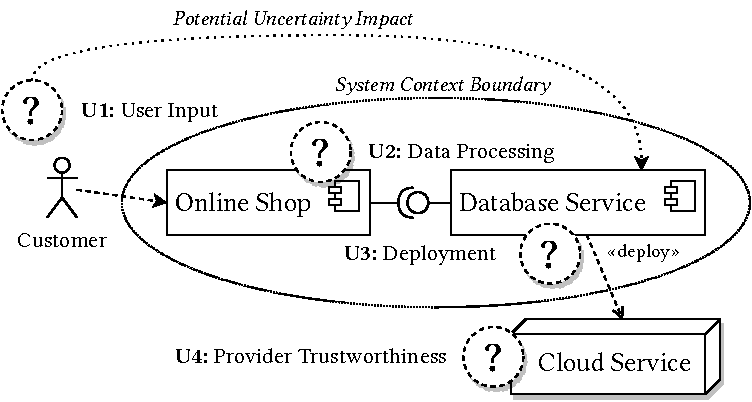
\includegraphics[width=0.8\textwidth]{figures/chapter5/onlineshop-context.pdf}
    \caption{Combined component and deployment diagram of the running example with annotated uncertainty sources, the system context boundary, and the impact of the user input uncertainty source.}
    \label{fig:classification:example}
\end{figure}


\subsection{Existing Notions of Uncertainty}

Multiple definitions of uncertainty exist, see \autoref{sec:foundations:uncertainty}.
Regarding software-architectural uncertainty, we consider two major points of view.
First, the concept of uncertainty stemming from the research community of \acp{SAS} \cite{weyns_towards_2023,weyns_introduction_2020}.
Here, uncertainty is often referred to as unanticipated change, fuzziness, noise, or incomplete knowledge \cite{weyns_towards_2023} and located within the system context or environment \cite{weyns_introduction_2020}.
Uncertainty is seen as a challenge which has to be considered within the system design and \enquote{engineering software-intensive systems that can handle uncertainty is complex} \cite{weyns_introduction_2020}.
Second, from a software engineering point of view, the \emph{cone of uncertainty} describes the inherent phenomenon of the lack of knowledge about a software system in early development phases \cite{mcconnell_software_1998}.
Here, uncertainty is constituted as part of every software project and is reduced over time, e.g., by making design decisions like \acp{ADD}.
In our running example, the user input (\U{1}) as human in the loop and the provider trustworthiness (\U{4}) as uncertain environment represent uncertainty sources known from \acp{SAS}.
Opposite to this, the data processing (\U{2}) and the deployment (\U{3}) represent design decisions that would reduce the \emph{cone of uncertainty}.
Regarding software-architectural uncertainty, we do not distinguish between these two perspectives, as both are relevant regarding confidentiality.
As long as we can represent the uncertainty sources in architectural models and analyze their impact, we can asses their effect on confidentiality.

When dealing with software-architectural uncertainty, considering \acp{ADD} helps to structure the design process.
At the beginning of this process, much is yet unknown or imprecise and \acp{ADD} are made under assumptions \cite{mcconnell_software_1998}, e.g., that the provider is trustworthy in Uncertainty \U{4}.
Making this uncertainty explicit can help to mark decisions as challenged \cite{kruchten_ontology_2004} and consider backtracking\footnote{A couple of years ago, I had the possibility to discuss this very point with Philippe Kruchten. He stressed the importance and costs of backtracking due to false assumptions and design faults. This was another motivation to research the early identification and impact analysis of software-architectural uncertainty.}.
While some uncertainty only exists due to not yet decided \acp{ADD}, others cannot be reduced immediately \cite{perez-palacin_uncertainties_2014}, e.g., Uncertainty \U{1} regarding the user input.
Still, creating awareness of the uncertainty source can help refine the architecture and make more informed statements about confidentiality.
This way, uncertainty can be understood, modeled, analyzed, and---eventually---managed.

There are multiple relevant properties of \acp{ADD} that help in the mitigation of uncertainty.
The number of solutions of related \acp{ADD} \cite{jansen_software_2005} can help to estimate whether the uncertainty can already be fully reduced at design time, e.g., by design space exploration \cite{esfahani_guidearch_2013,koziolek_peropteryx_2011}.
We distinguish between closed sets that could at least partially be analyzed and open sets with a potentially infinite number of solutions or configurations.
In our example, Uncertainty \U{3} relates to the \ac{ADD} of the deployment of the \emph{Database Service} and represents a closed set.
But even with a closed set of alternatives, one cannot guarantee that a given \ac{ADD} might not be challenged in the future \cite{kruchten_ontology_2004} due to changes in requirements or the system's execution context.
Thus, when speaking about decisions under uncertainty, considering the probability, possibility and costs of revisions can help to quantify the risk.
This awareness also helps in the prioritization of \acp{ADD} and deciding whether existing mitigation is sufficient.

However, only considering \acp{ADD} to understand the impact of uncertainty is not enough because uncertainty might not be directly connected to a single decision, e.g., to resolve Uncertainty \U{4}.
We argue to also consider which architectural elements are affected, rather than only considering this transitively via the impact of \acp{ADD}.
This does help in understanding the consequences of uncertain influences regarding confidentiality and also helps to connect these to architectural analyses to identify confidentiality violations.

\finding{%
Different notions of uncertainty exist, e.g., the \emph{cone of uncertainty} or uncertainty in \acfp{SAS}.
We do not limit software-architectural uncertainty to one of these notions, as all of these uncertainties can affect confidentiality.
Regarding the software architecture, considering \acfp{ADD} helps for early assessment and prioritization.}


\subsection{Investigating Existing Uncertainty Classifications}%
\label{sec:classification:investigating}

Based on our understanding of the relation of uncertainty, software architecture, and confidentiality presented in the previous section, we investigate existing uncertainty classifications stemming from related work.
Hereby, we address Problem \PR{1}{2} regarding the need for a classification tailored to confidentiality.
As discussed previously and also in \autoref{sec:foundations:uncertainty}, there are many types, notions, and dimensions of uncertainty.
In the following, we follow a top-down approach by discussing shortcomings of classifications and taxonomies while focusing on confidentiality.

We gathered and assessed categories, i.e., dimensions, or characteristics, and options, i.e., entries of a category in \autoref{sec:foundations:uncertainty}.
Here, the first category was the \emph{location} of uncertainty, see \autoref{table:foundations:sources:locationlevel}.
Although this category is used in many taxonomies \cite{bures_capturing_2020,mahdavi-hezavehi_classification_2017,perez-palacin_uncertainties_2014,walker_defining_2003,troya_uncertainty_2021,PSUM}, is has several shortcomings. 
There is no common distinction between the source and the impact location of uncertainty.
Also, there is no common understanding of the term \emph{model} as the taxonomies originate from different research areas.
This impedes the common understanding of uncertainty regarding confidentiality.
In the running example, Uncertainty \U{3} about the deployment could be classified as \emph{context}, \emph{model structural}, \emph{model technical}, and \emph{belief uncertainty}.
Such ambiguity can invalidate the purpose of a classification.
The second category was the \emph{level} of uncertainty, see \autoref{table:foundations:sources:locationlevel}. 
In the running example, all uncertainty sources represent known unknowns, i.e., first-order uncertainty, because we are aware of the sources and can annotate them in the architectural model.
However, the concrete representation might be different, e.g., using scenarios to describe the deployment of Uncertainty \U{3}.
As discussed previously, we find distinguishing between a \emph{known} and \emph{unknown} uncertainty to be not expedient as it only depends on the viewpoint of the software architects whether they are aware of the uncertainty source.

The next three categories are the \emph{nature}, \emph{manageability}, and the \emph{resolution time}, see \autoref{table:foundations:sources:naturemanagetime}.
In our running example, the uncertainty sources in the software system, i.e., Uncertainty \U{2} about the data processing and Uncertainty \U{3} about the deployment, represent epistemic uncertainty.
The uncertainty sources in the system context, i.e., Uncertainty \U{1} about the user input and Uncertainty \U{4} about the provider trustworthiness can be classified as epistemic or aleatory, depending on the point of view.
This shows again the ambiguity of this category.
All uncertainties in the running example can be described using scenarios and resolved between design and run time.

The last categories are the \emph{impact on quality} of uncertainty and the \emph{relationships} between uncertainties.
To focus analysis capabilities, software architects must know about potential impacts and their severity.
Although we focus on confidentiality, the analysis of multiple properties is possible, e.g., by using software architecture evaluation approaches under uncertainty \cite{sobhy_evaluation_2021}.
In the running example, all four uncertainty sources can have an impact on confidentiality.
Uncertainty relationships can cause hard-to-find problems regarding quality properties \cite{camara_addressing_2022}.
However, they often require further analysis based on the software system under study \cite{camara_uncertainty_2024}.
In the running example, there is such a relationship between Uncertainty \U{3} about the deployment and Uncertainty \U{4} about the provider's trustworthiness.
The latter only affects the confidentiality of the software system if the cloud provider is chosen in the first place.
As described above, such uncertainty interactions have to be further analyzed \cite{camara_uncertainty_2024}, and cannot be generally described using a classification.

\finding{The literature comprises many classifications and taxonomies of uncertainty that propose categories like location, level, or nature.
Despite being mostly relevant regarding confidentiality, they use varying terminology, contain ambiguity, and do not focus on uncertainty sources.
Thus, they have to be adapted to classify software-architectural uncertainty sources.}





\section{Classification of Uncertainty Regarding Confidentiality}%
\label{sec:classification:classification}

Based on the categories and options we identified in existing classifications of uncertainty, we define a novel classification scheme of uncertainty regarding confidentiality.
This allows us to build on existing knowledge from the domain of \acp{SAS} while aligning the classification to software-architectural uncertainty and confidentiality.
Additionally, we focus on uncertainty \emph{sources} as the primary concern regarding identification and early mitigation \cite{ramirez_taxonomy_2012,perez-palacin_uncertainties_2014}, see \autoref{sec:classification:relation}.
This addresses our second Problem \PR{1}{2} regarding the need for a classification tailored to confidentiality.

Our classification scheme consists of 8 categories with a total of 27 options and is shown in the tables \ref{table:classification:classification:location} -- \ref{table:classification:classification:severityoftheimpact}.
The categories are based on taxonomies of uncertainty \cite{bures_capturing_2020,esfahani_uncertainty_2013,mahdavi-hezavehi_classification_2017,perez-palacin_uncertainties_2014,ramirez_taxonomy_2012,walker_defining_2003,PSUM}, related work on \acp{ADD} \cite{jansen_software_2005,kruchten_ontology_2004} and \acp{ADL} like the \ac{PCM} \cite{reussner_modeling_2016}.
A category-based classification helps to group uncertainties and identify similar characteristics and mitigation approaches.
Once classified, the information can be reused across different software architectures.
To create this classification, we assessed and adapted existing categories and combined or refined their options, see \autoref{sec:classification:investigating}.
We repeated this process until each category fulfilled its purpose, i.e., being able to describe and partition uncertainty sources with respect to confidentiality in software architectures.

In this work, we focus on confidentiality requirements during the design time. 
Thus, the categories should be interpreted from an architectural point of view, e.g., while modeling a software system. 
In the following, we explain each category in detail.
We provide information about the rationale and possible benefits of applying each category.
We also define whether the options are unordered, i.e., \emph{nominal}, or ordered without defined distance, i.e., \emph{ordinal}.
Last, we specify if the gained knowledge by classification can be reused.
Here, a category can be specific for the uncertainty source and thus \emph{system-independent}, or specific for the software architecture under investigation and thus \emph{system-specific}.
This also concerns the question of whether the specific classification of a source of uncertainty is \emph{immutable} and does not change after the identification or \emph{mutable} and can be changed if more information is obtained during modeling and analysis.


\subsection{Classification Category: Location}

\begin{table}
    \begin{tabularx}{\textwidth}{lX}
        \toprule
        \tableheading{Location}{Describes where an uncertainty manifests itself within the architecture\\and which view or concern of the software architecture is primarily applicable.\\ \classificationtags{System-Independent}{Nominal}{Immutable}}
        \midrule
        \tableentry{System Structure}{The uncertainty is related to the structure of the software system and becomes visible in structural views, e.g., component diagrams, or class diagrams.}
        \tableentry{System Behavior}{The uncertainty is related to the behavior of the software system and becomes visible in behavioral views, e.g., activity diagrams, or sequence diagrams.}
        \tableentry{System Environment}{The uncertainty is related to the environmental context of the software system and becomes visible when considering external factors, e.g., in deployment diagrams.}
        \tableentry{System Input}{The uncertainty is related to the input to the software system and becomes visible when considering external interface specifications, or usage descriptions.}
        \bottomrule
    \end{tabularx}
    \caption{Uncertainty classification regarding confidentiality. Category: Location.}%
    \label{table:classification:classification:location}
\end{table}

The first category shown in \autoref{table:classification:classification:location} is concerned with the \emph{location} of the uncertainty source.
Previous taxonomies \cite{bures_capturing_2020,mahdavi-hezavehi_classification_2017,perez-palacin_uncertainties_2014,walker_defining_2003} already considered \enquote{where the uncertainty manifests itself within the model} \cite{perez-palacin_uncertainties_2014} but did not explicitly relate to an \ac{ADL}.
Since the location of the source is one of the most important properties for design time modeling analysis, we define four locations as inspired by the viewpoints of the PCM \cite{reussner_modeling_2016}.
Compared to existing taxonomies, this enables more precise description and mitigation because we can model uncertainty and its relation to existing architecture elements.

The option \emph{system structure} describes uncertainty in components and their assembly, which becomes visible in structural views like component diagrams.
The option \emph{system behavior} describes uncertainty in the communication, e.g., related to the handling of data within a component or the communication between components.
The option \emph{system environment} describes uncertainty in the system's context including hardware resources and the external situation.
The option \emph{system input} describes uncertainty in inputs provided by external actors, e.g., people using the software system.
Note that we distinguish between the input, i.e., the user behavior, and the system behavior.
This is due to the special role---and rights---of humans with regard to confidentiality, e.g., due to legal requirements like the \ac{GDPR} \cite{council_of_european_union_regulation_2016}, and shall also help in collaboration with legal analysis \cite{boltz_model-based_2022}.
Because the location is defined on the level of an \ac{ADL} meta model, it is system-independent and immutable.
The category is nominal, as its options only represent viewpoints without applicable order.


\subsection{Classification Category: Architectural Element Type}

\begin{table}
    \begin{tabularx}{\textwidth}{lX}
        \toprule
        \tableheading{Architectural Element Type}{Describes the type or class of elements to which an\\uncertainty can be assigned when considering its impact on a software system's\\confidentiality. \classificationtags{System-Independent}{Nominal}{Immutable}}
        \midrule
        \tableentry{Component}{The uncertainty is assignable to software components. This represents the nodes of a software system.}
        \tableentry{Connector}{The uncertainty is assignable to wires between components, or their communication. This represents the edges between the nodes of a system.}
        \tableentry{Interface}{The uncertainty is assignable to interfaces of components. This represents the contact point of nodes and edges in a software system.}
        \tableentry{External}{The uncertainty is assignable to external resources or their properties. This represents annotating the nodes of a software system.}
        \tableentry{Behavior}{The uncertainty is assignable to behavior descriptions. This represents specifying the behavior of nodes within a software system.}
        \bottomrule
    \end{tabularx}
    \caption{Uncertainty classification regarding confidentiality. Category: Architectural Element Type.}%
    \label{table:classification:classification:architecturalelementtype}
\end{table}

\autoref{table:classification:classification:architecturalelementtype} shows the second category \emph{Architecture Element Type}.
While the \emph{Location} is on the abstraction of the viewpoint (e.g., structure, or behavior), the \emph{Architecture Element Type} describes the concrete elements where the uncertainty arises.
Similarly to the previous category, the options are inspired by software architecture element types known from \acp{ADL} like the \ac{PCM}.
We consider this to be the central category for further modeling and analysis of uncertainty, as it specifies a starting point to consider the effect of an uncertainty source.
Compared to existing classifications, we provide five concrete options rather than only speaking of uncertainty within the model \cite{perez-palacin_uncertainties_2014}.
The need for such precision is supported by more recent approaches to classifying and propagating uncertainty \cite{acosta_uncertainty_2022,camara_uncertainty_2024} and also in the recent \ac{PSUM} standard \cite{PSUM}.
By understanding which elements and viewpoints are affected, software architects can assess responsibilities and evaluate mitigation methods.

The option \emph{component} describes uncertainty assignable to software components, e.g., related to their allocation or other component-wide decisions or properties.
The option \emph{connector} describes uncertainty assignable to, e.g., wires between components and thus communication and its properties.
The option \emph{interface} describes uncertainty assignable to interfaces, e.g., signatures, parameters, and return values.
The option \emph{external} describes uncertainty assignable to hardware resources, e.g., servers, and external actors like users of the system.
Note that we renamed this category compared to the original publication \cite{hahner_classification_2023} to take into account that users also represent external entities.
The option \emph{behavior} describes uncertainty assignable to behavior descriptions, e.g., algorithms, user behavior and input, data processing, and persistence.
This option also helps to underline the difference between \emph{Architecture Element Type} and \emph{Location}: Although behavior descriptions of users and the software system may be similar, the viewpoints of \emph{System Behavior} and \emph{System Input} are different.
Both categories are orthogonal and cannot be replaced by each other.
The category is immutable and system-independent and can thus be reused across architectural models.
The category is nominal as there is no order between location or element types.


\subsection{Classification Category: Type}

\begin{table}
    \begin{tabularx}{\textwidth}{lX}
        \toprule
        \tableheading{Type}{Describes how much is known about uncertainty and how it is described\\on a scale from only being aware to having precise knowledge. This may change\\with growing knowledge. \classificationtags{System-Specific}{Ordinal}{Mutable}}
        \midrule
        \tableentry{Statistical Uncertainty}{The uncertainty can be described with statistical means, e.g., related to the probability of certain outcomes.}
        \tableentry{Scenario Uncertainty}{The uncertainty can be described with distinct scenarios but there is a lack of knowledge to apply statistical means.}
        \tableentry{Recognized Ignorance}{There is awareness of the uncertainty but no knowledge about potential scenarios or lack of a description strategy. This is the most general form of an identfied uncertainty source.}
        \bottomrule
    \end{tabularx}
    \caption{Uncertainty classification regarding confidentiality. Category: Type.}%
    \label{table:classification:classification:type}
\end{table}

The third category is called \emph{Type} and describes how much is known about the uncertain influence as shown in \autoref{table:classification:classification:type}.
Other taxonomies \cite{bures_capturing_2020,perez-palacin_uncertainties_2014} only specify this in terms of levels on a scale from knowledge to ignorance \cite{armour_five_2000}, which is too imprecise to classify uncertainty for later mitigation.
With the \emph{Type}, we describe how much is known about the uncertainty, based on the definitions by Walker et al. \cite{walker_defining_2003}.
As discussed previously, we do distinguish between known or unknown unknowns as this depends on the viewpoint of the software architect and not the classified uncertainty source.

\emph{Statistical} uncertainty implies that the uncertainty is describable with statistical means, e.g., stochastic expressions, or probability distributions.
\emph{Scenario} uncertainty implies that the uncertainty can be represented with distinct scenarios depending on the uncertain outcome but without statistical means.
\emph{Recognized ignorance} only implies awareness of uncertainty sources, without scenario-based or statistical means to describe their form. 
These options can be ordered depending on the amount of knowledge and thus are ordinal.
Having statistical information enables more precise analysis results than just knowing scenarios---which is still better than simple awareness.
The category is system-specific and mutable.
During the software design and realization, more information may be gained, enabling a more precise description of the uncertainty, e.g., because more statistical information is collected or some scenarios can be excluded.


\subsection{Classification Category: Manageability}

\begin{table}
    \begin{tabularx}{\textwidth}{lX}
        \toprule
        \tableheading{Manageability}{Describes to which extent the uncertainty can be managed, reduced,\\or mitigated. This only provides a first estimate and may change with growing\\knowledge. \classificationtags{System-Specific}{Ordinal}{Mutable}}
        \midrule
        \tableentry{Fully Reducible}{The uncertainty can be fully resolved with appropriate means that mitigate its potential impact.}
        \tableentry{Partially Reducible}{The uncertainty is at least partially reducible which reduces the potential impact severity or limits critical outcomes by appropriate mitigation techniques.}
        \tableentry{Irreducible}{The uncertainty cannot be further reduced as there is no reasonable way to achieve the required knowledge at this point in time.}
        \bottomrule
    \end{tabularx}
    \caption{Uncertainty classification regarding confidentiality. Category: Manageability.}%
    \label{table:classification:classification:manageability}
\end{table}

The fourth category shown in \autoref{table:classification:classification:manageability} covers the \emph{manageability} of uncertainty.
\emph{Manageability} states whether we can control or reduce the impact of the uncertainty at design time or are only aware of it \cite{esfahani_uncertainty_2013}.
Early identification of potential threats to security-related properties like confidentiality is also required by \emph{Data Protection by Design} \cite[Art.~25]{council_of_european_union_regulation_2016}. 
We do not consider the nature of the uncertainty \cite{walker_defining_2003} because the manageability is closer to the uncertainty's impact on the software system \cite{esfahani_uncertainty_2013}.
Representing the manageability on a scale from reducibility to irreducibility is also supported by the \ac{PSUM} standard \cite{PSUM}.

\emph{Fully reducible} uncertainty can be fully reduced by taking appropriate actions, e.g., an \ac{ADD} at design time, or comprehensive simulation. This can include \enquote{collecting additional information until achieving full certainty} \cite{PSUM}.
\emph{Partially reducible} implies that full certainty cannot be reached.
Nevertheless, the uncertainty can be reduced by collecting more information, or by applying scenario-based mitigation strategies, or system-wide constraints and policies.
\emph{Irreducible} uncertainty cannot be further reduced, e.g., due to its aleatory nature \cite{perez-palacin_uncertainties_2014,PSUM}.
Similar to the type category, this category is ordinal because the options can be ordered.
The classification depends on the architecture under investigation and the current knowledge.
Thus, this option is system-specific and mutable.
However, many uncertainty types tend to be categorized similarly across architectures.


\subsection{Classification Category: Resolution Time}

\begin{table}
    \begin{tabularx}{\textwidth}{lX}
        \toprule
        \tableheading{Resolution Time}{Describes the rough time span in the development process where\\the uncertainty is usually expected to be fully resolved.\\ \classificationtags{System-Independent}{Ordinal}{Immutable}}
        \midrule
        \tableentry{Requirements Time}{The uncertainty is expected to be resolved as soon as the requirements are defined.}
        \tableentry{Design Time}{The uncertainty is expected to be resolved as soon as the software system is designed.}
        \tableentry{Realization Time}{The uncertainty is expected to be resolved as soon as the software system or parts of it are implemented and deployed.}
        \tableentry{Runtime}{The uncertainty is expected to be resolved as knowledge is gained from testing and system operations, or not at all.}
        \bottomrule
    \end{tabularx}
    \caption{Uncertainty classification regarding confidentiality. Category: Resolution Time.}%
    \label{table:classification:classification:resolutiontime}
\end{table}

The \emph{Resolution Time} shown in \autoref{table:classification:classification:resolutiontime} is based on the phases of software development and can help to narrow down sources and responsibilities.
Since we focus on the impact of uncertainty on confidentiality, we consider the expected full resolution time rather than the emerging time \cite{hezavehi_uncertainty_2021,perez-palacin_uncertainties_2014,ramirez_taxonomy_2012,troya_uncertainty_2021}.
Also, we only include phases that are relevant from the point of view of design time modeling and analysis.

\emph{Requirements time} implies that the uncertainty resolves as soon as requirements are defined, e.g., related to confidentiality requirements or security policies.
\emph{Design time} implies that the uncertainty resolves as soon as the system is designed, e.g., because the uncertainty is related to \acp{ADD}, the system structure, or software components.
\emph{Realization time} implies that the uncertainty resolves as the system or parts of it are implemented and deployed.
Here, we combine implementation and deployment as a distinction is not expedient from an architectural point of view.
\emph{Runtime} implies that the uncertainty resolves at runtime, e.g., because knowledge is gained from testing or dynamic analysis like monitoring or profiling.
This category depends on the uncertainty source and not on the system under study and is thus system-independent and immutable.
It is ordinal because we can order the options along the phases of software development from requirements to runtime.


\subsection{Classification Category: Reducible by ADD}

\begin{table}
    \begin{tabularx}{\textwidth}{lX}
        \toprule
        \tableheading{Reducible by ADD}{Describes whether the uncertainty is resolvable or treatable by\\an architectural design decision, i.e., a decision that specifies or restricts a software\\systems's structure or behavior, thereby limiting the design space.\\ \classificationtags{System-Independent}{Nominal}{Immutable}}
        \midrule
        \tableentry{Yes}{The uncertainty can be reduced by making an architectural design decision.}
        \tableentry{No}{The uncertainty is not resolvable by taking an architectural design decision.}
        \bottomrule
    \end{tabularx}
    \caption{Uncertainty classification regarding confidentiality. Category: Reducible by ADD.}%
    \label{table:classification:classification:reduciblebyadd}
\end{table}

\autoref{table:classification:classification:reduciblebyadd} shows the category \emph{Reducible by ADD} that specifies whether the uncertainty source can at least be partially mitigated by a design decision on architectural abstraction, i.e., an \ac{ADD}.
Making the connection between \acp{ADD} and uncertainty explicit \cite{lytra_supporting_2013} helps to prioritize, e.g., check whether multiple or critical uncertainty sources can be tackled by a single decision.
\acp{ADD} are seen as crucial aspect of software architecture \cite{jansen_software_2005,kruchten_ontology_2004,alexeeva_design_2016}. 

The option \emph{Yes} describes uncertainty which can be addressed on architectural abstraction by making appropriate decisions, i.e., by designing the system in a way that the impact of the uncertainty is (partially) mitigated
This implies that the uncertainty can---and probably should---be addressed in the architectural design and falls into the \emph{cone of uncertainty} \cite{mcconnell_software_1998}.
The option \emph{No} describes uncertainty that is not resolvable or treatable by taking an \ac{ADD}, e.g., because the uncertainty is outside the scope of the designed software system, or cannot be properly addressed within the design process, e.g., due the behavior of a third-party.
An uncertainty that is not resolvable by an \ac{ADD} does not imply a resolution later than design time.
The uncertainty could also exist due to a lack of knowledge or could be addressed on a lower level than architectural abstraction---but not by an \ac{ADD}.
Both categories are orthogonal.
Reducibility is nominal, system-independent and immutable.


\subsection{Classification Category: Impact on Confidentiality}

\begin{table}
    \begin{tabularx}{\textwidth}{lX}
        \toprule
        \tableheading{Impact on Confidentiality}{Describes the impact on confidentiality requirements.\\Initially, this only provides a first, system-independent estimate.\\ \classificationtags{System-Specific}{Ordinal}{Mutable}}
        \midrule
        \tableentry{Direct}{The uncertainty has a direct impact on the software system's confidentiality.}
        \tableentry{Indirect}{The uncertainty only has an indirect impact on the software's confidentiality that usually relies on other uncertainties or other contextual factors.}
        \tableentry{None}{The uncertainty is expected to have no impact on confidentiality at all.}
        \bottomrule
    \end{tabularx}
    \caption{Uncertainty classification regarding confidentiality. Category: Impact on Confidentiality.}%
    \label{table:classification:classification:impactonconfidentiality}
\end{table}

The last two categories are used to quantify the impact of uncertainty on confidentiality requirements.
\autoref{table:classification:classification:impactonconfidentiality} shows the category \emph{Impact on Confidentiality}.
It represents a first estimate on whether the uncertainty can directly impact confidentiality or requires additional conditions to result in confidentiality violations.

The option \emph{Direct} describes uncertainty with a direct impact that can void confidentiality even without taking other factors, decisions, or uncertainties into account, e.g., by directly affecting input, processing, or storage of sensitive data like user data.
The option \emph{Indirect} describes uncertainty that is related to \acp{ADD}, security measures, or other uncertainty sources.
The option \emph{None} describes uncertainty without impact on confidentiality, e.g., if it is related to handling non-sensitive data or well-secured system parts or because the uncertainty has no effect on any data processing at all, e.g., related to the color of a button.
Note that this category only describes the type of impact but not its severity.
An indirect impact can be as severe as a direct impact but is potentially even harder to identify.
This category only provides a first, mutable estimate and is highly system-specific.
We consider the options to be ordinal as they can be sorted from direct to no impact.


\subsection{Classification Category: Severity of the Impact}

\begin{table}
    \begin{tabularx}{\textwidth}{lX}
        \toprule
        \tableheading{Severity of the Impact}{Describes the severity if the uncertainty is not mitigated.\\Initially, this only provides a first, system-independent estimate.\\ \classificationtags{System-Specific}{Ordinal}{Mutable}}
        \midrule
        \tableentry{High}{The uncertainty can cause a total loss of confidentiality, e.g. due to a data breach.}
        \tableentry{Low}{The uncertainty can cause information leaks, but the damage is limited.}
        \tableentry{None}{The uncertainty is expected to cause no loss of confidentiality at all.}
        \bottomrule
    \end{tabularx}
    \caption{Uncertainty classification regarding confidentiality. Category: Severity of the Impact.}%
    \label{table:classification:classification:severityoftheimpact}
\end{table}

To prioritize uncertainty with a potentially critical impact, we combine the previously introduced impact type with its severity.
\autoref{table:classification:classification:severityoftheimpact} shows the last category of the classification that is named \emph{Severity of the Impact}.
This category is based on the confidentiality impact metrics of the open industry standard \acf{CVSS} \cite{CVSS}.
We reuse the definition as it is broadly used, and known by security experts.

The option \emph{High} refers to uncertainty that can cause the total loss of confidential data or access to restricted information.
This can be the case because the uncertainty is either related to highly sensitive data like certificates, encryption keys, or an admin password or because the uncertainty is related to central security measures like input validation and sanitization.
The option \emph{Low} refers to uncertainty that could cause the loss of restricted information, but the damage is limited, e.g., because the input validation only has limited effects due to insufficient security policies.
The option \emph{No} refers to uncertainty where no loss of confidentiality is expected at all, e.g., because the uncertainty is related to parts of a software system that do not deal with sensitive information.
As stated in the previous category, there is no clear dependency between an impact's type and its severity.
Only uncertainty sources that have no impact on confidentiality at all are also expected to have no severity.
Other than that, any combination of high or low, and direct or indirect can happen. 
This category as well provides a first, mutable estimate that is system-specific.
Nevertheless, both categories help to estimate the potential impact and plan further steps toward analyzing the uncertainty. 
The knowledge gained by this classification can help in clustering and prioritizing uncertainty and related \acp{ADD}.
This category is ordinal.


\subsection{Building on the Uncertainty Classification}

In sum, our classification provides eight categories that do not classify uncertainty in isolation but also relate the uncertainty sources to software architecture and confidentiality, as discussed in \autoref{sec:classification:relation}.
These categories help in the early understanding of uncertainty sources and serve the discussion of software architects and security experts.
We split the categories into system-independent and system-specific.
System-specific categories are always mutable, as the knowledge about the uncertainty source can change over time.

\finding{Uncertainty classifications are a well-suited entry point to understanding uncertainty sources.
However, classification can change over time when more knowledge is gained or the system or environment changes.
Some categories of the classification depend on the architecture under study.
Still, many uncertainty sources tend to be categorized similarly across architectures.}

This classification represents the baseline for further modeling and analysis activities, as outlined in \autoref{sec:overview:procedure}.
Many categories help in the early assessment of the criticality of an uncertainty source, even without systematically analyzing the software architecture.
However, to gain detailed insights on the impact of uncertainty and to identify confidentiality violations, architecture-based analysis is expedient.
Here, we benefit from the category \emph{Architectural Element Type}, which relates uncertainty sources to concrete element types of software architectures and can be used to extend existing \acp{ADL} like the \ac{PCM}.

\finding{Centering an uncertainty classification around the location of the uncertainty source simplifies the later modeling, analysis, and mitigation.
Thus, we see the category \emph{Architectural Element Type} and its options \emph{Component}, \emph{Connector}, \emph{Interface}, \emph{External}, and \emph{Behavior} as central dimension of our classification.}

This finding is supported by comparable approaches \cite{acosta_uncertainty_2022,camara_uncertainty_2024} that analyze the impact of uncertainty.
\textcite{acosta_uncertainty_2022} define the category \emph{Locus} that describes the location of uncertainty within the model and serves as starting point of uncertainty propagation.
Due to the importance of this category, we will use it throughout the remainder of this thesis and refer to it directly, e.g., by speaking of \emph{Component} uncertainty, \emph{Behavior} uncertainty, or \emph{External} uncertainty.





\section{Applying the Classification to the Running Example}%
\label{sec:classification:runningexample}

We illustrate the classification introduced in the previous section by applying it to the running example from \autoref{ch:runningexample}.
The running example, which shows a simplified online shop, comprises four uncertainties: The user input, data processing within the \emph{Online Shop} component, the deployment of the \emph{Database Service}, and the provider trustworthiness of the \emph{Cloud Service} resource.
In the following, we present one possible classification using the aforementioned classification scheme.
While some categories like the location are system-independent, others like the severity regarding confidentiality are system-specific and are based on our interpretation of the running example.
We provide our reasoning and also explain alternative classifications.
All classified uncertainty sources are part of our data set \cite{dataset}.
Additionally, they are listed in \arcen with the proposed classification\footnote{At the time of writing, \arcen is online available here: \url{https://arc3n.abunai.dev/}. Currently, the uncertainty sources of the running example \U{1} -- \U{4} are listed as \href{https://arc3n.abunai.dev/uncertainty/52}{\#52}, \href{https://arc3n.abunai.dev/uncertainty/35}{\#35}, \href{https://arc3n.abunai.dev/uncertainty/59}{\#59}, and \href{https://arc3n.abunai.dev/uncertainty/48}{\#48}.}.


\begin{table}
    \centering
    \begin{tabular}{lll}
        \toprule
        Category                        & \U{1}: User Input   & \U{2}: Data Processing \\
        \midrule
        Location                        & System Input              & System Behavior \\
        Architectural Element Type\;    & Connector                 & Behavior \\
        Type                            & Scenario Uncertainty\;    & Scenario Uncertainty \\
        Manageability                   & Partially Reducible       & Fully Reducible \\
        Resolution Time                 & Runtime                   & Design Time \\
        Reducible by ADD                & Yes                       & Yes \\
        Impact on Confidentiality       & Indirect                  & Direct \\
        Severity of the Impact          & High                      & High \\
        \bottomrule
    \end{tabular}
    \caption{Exemplary classification of the uncertainty sources U1 and U2 in the running example.}%
    \label{table:classification:example:one}
\end{table}

\autoref{table:classification:example:one} shows our classification of the first two uncertainty sources, i.e., the user input (\U{1}) and the data processing (\U{2}).
The Uncertainty \U{1} about the user input is located in the system input and can be annotated at a connector.
We annotate the uncertainty to a connector instead of a behavior description because it relates to the question of how the user communicates with the system.
In our discussion in \autoref{sec:runningexample:uncertainty}, we enumerated scenarios like normal or malicious behavior, thus we already reached the knowledge of scenario uncertainty.
With mitigation strategies like proper input validation, we can at least partially reduce the uncertainty---more optimistic experts could even argue for full reducibility.
The uncertainty persists until run time when actual humans use the system under study.
Until then, it is reducible by appropriate design decisions like the aforementioned input validation.
The input on confidentiality in our example is indirect as it depends on the data processing, and thus, it depends on Uncertainty \U{2} whether confidentiality could be violated.
If we do not have any means of input validation, the impact could be direct.
We classify the severity as high because confidentiality cannot be guaranteed under this uncertainty.

The Uncertainty \U{2} about the data processing is located in the system behavior and can be represented in a behavior description.
Similarly to Uncertainty \U{1}, we already provided scenarios in \autoref{sec:runningexample:uncertainty}, thus, it represents scenario uncertainty.
The uncertainty about the data processing is an uncertainty due to an open \ac{ADD} as described by the \emph{cone of uncertainty} \cite{mcconnell_software_1998}.
Thus, it is fully reducible already at design time.
We classify the impact on confidentiality as direct and high, because improper processing directly and severely affects the confidentiality, e.g., because of missing validation or encryption.


\begin{table}
    \centering
    \begin{tabular}{lll}
        \toprule
        Category                        & \U{3}: Deployment   & \U{4}: Provider Trustworthiness \\
        \midrule
        Location                        & System Structure          & System Environment \\
        Architectural Element Type\;    & Component                 & External \\
        Type                            & Scenario Uncertainty\;    & Scenario Uncertainty \\
        Manageability                   & Partially Reducible       & Partially Reducible \\
        Resolution Time                 & Realization Time          & Runtime \\
        Reducible by ADD                & Yes                       & Yes \\
        Impact on Confidentiality       & Direct                    & Indirect \\
        Severity of the Impact          & High                      & High \\
        \bottomrule
    \end{tabular}
    \caption{Exemplary classification of the uncertainty sources U3 and U4 in the running example.}%
    \label{table:classification:example:two}
\end{table}

\autoref{table:classification:example:two} shows our classification of the last two uncertainty sources, i.e., the deployment (\U{3}) and the provider trustworthiness (\U{4}). 
The Uncertainty \U{3} about the deployment is located in the system structure and can be annotated to a component that must be deployed.
In \autoref{sec:runningexample:architecture}, we describe two scenarios of this scenario uncertainty, i.e., deployment on premise, or in the cloud.
In our interpretation, this uncertainty is only partially reducible by a proper \ac{ADD} at design time as it resolves at realization time, i.e., when the component gets deployed after the architectural design of the software system.
In our running example, the impact on confidentiality is direct and high.
If the confidentiality requirements demand selected deployment locations due to legal requirements like the \ac{GDPR} \cite{council_of_european_union_regulation_2016}, any deviation causes a confidentiality violation.

The Uncertainty \U{4} about the trustworthiness of the cloud service provider is located in the system environment and classified as external uncertainty in the system's context, see \autoref{fig:classification:example}.
Although we cannot control the provider's behavior, we can describe scenarios, i.e., trustworthy or not trustworthy behavior.
With further knowledge or experience, experts could quantify the probability of these scenarios to reach statistical uncertainty, but in the running example, that is out of scope.
With proper \ac{ADD}, we can at least limit the impact of this uncertainty.
Thus, it is partially reducible.
In our running example, the impact on confidentiality is high but indirect.
The impact depends on the form of data processing (\U{2}) and also the deployment location (\U{3}).
Put simply, the cloud provider's trustworthiness does not affect the confidentiality if nothing is deployed in the cloud.

In sum, this illustration shows how our classification can be applied to better understand uncertainty sources.
Compared to other classifications, we focus on confidentiality and thus provide appropriate categories for this purpose\footnote{I discussed this question with Raffaela Mirandola, who co-authored one of the investigated classifications \cite{perez-palacin_uncertainties_2014}. We concluded that there is no such thing as a \emph{best} classification---only appropriate and less appropriate classifications for a specific \emph{purpose}.}.
Describing the uncertainty in these categories helps to better understand the relation and criticality of uncertainty sources.
In our running example, we can see the importance of proper data processing (\U{2}) even without applying automated architectural analyses.
We also see the importance of choosing the right deployment locations and can prioritize this \ac{ADD}.
Last, classifying uncertainty always has some level of interpretation.
Thus, the classification of similar uncertainty sources in other software systems could be different.
Moreover, our classification could change at a later stage, e.g., when enough knowledge about the uncertainty sources and the probability of certain scenarios is gained for statistical analysis.





\section{Representing Uncertainty in Data Flow Diagrams}%
\label{sec:classification:dfd}

Analyzing confidentiality with \acfp{DFD} \cite{tuma_flaws_2019,schneider_automatic_2023,seifermann_detecting_2022} has been proposed because \enquote{problems tend to follow the data flow, not the control flow} \cite{shostack_threat_2014}.
Thus, Problem \PR{1}{3} is concerned with the representation of uncertainty in \acp{DFD}.
We address this by connecting \acp{DFD} to the \emph{Architectural Element Type} category of our classification.
As concluded previously in \autoref{sec:classification:classification}, this category is crucial for modeling and analyzing uncertainty on architectural abstraction.
This applies to \acp{ADL} like the \ac{PCM} \cite{reussner_modeling_2016} as well as to \acp{DFD}.
The following section builds on the foundations about \acp{DFD}, \acp{DAG}, and the unified modeling primitives \cite{seifermann_unified_2021} presented in \autoref{sec:foundations:dfd}.


\subsection{Mapping Uncertainty to Data Flow Diagrams}

\acp{DFD} consist of processes, data flows, files, data sources, and data sinks---put simply, different types of nodes and edges.
The unified modeling primitives \cite{seifermann_unified_2021} extend this notation and consist of nodes, pins, flows, behavior and labels with their assignments.
Nodes represent structural elements of software systems, e.g., processes, stores, or external entities.
Pins represent their interfaces and flows are used to connect multiple nodes through their pins.
Nodes have a defined behavior that assigns labels, e.g., based on labels at the node's input pins, constants, logical expressions or a combination of the above.
In our running example presented in \autoref{ch:runningexample}, we can represent the data processing of the \emph{Online Shop} component as a process node.
The node has one input pin for the incoming data flow from the user and one output pin for the outgoing, processed data flowing to the \emph{Database Service}.
The deployment of the \emph{Online Shop} component can be represented as a \emph{On Premise} label that is assigned to the process node.
Last, the behavior of the data processing node can be described using an assignment that assigns the label \emph{Encrypted} to all outgoing data to represent the encryption of all processed data.
For details on the unified modeling primitives of \acp{DFD}, see \autoref{sec:foundations:dfd} or the primary publication \cite{seifermann_unified_2021}.

In \autoref{table:classification:classification:architecturalelementtype}, we describe the category \emph{Architectural Element Type} which comprises the options component, connector, interface, external, and behavior.
Speaking in terms of nodes and edges, these options represent uncertainty, e.g., within a node in the case of component uncertainty, or at the contact point of a node and an edge in the case of interface uncertainty.
We build on this finding and the fact that \acp{DFD} are a viable representation of software architectures \cite{schneider_how_2024} to map the five uncertainty types to \acp{DFD}. 
\autoref{table:classification:mapping} shows the mapping of the five uncertainty types of the category \emph{Architectural Element Type} to the unified modeling primitives.


\begin{table}
    \centering
    \begin{tabular}{lll}
        \toprule
        Uncertainty Type \, & Modeling Primitives \, & Effect of the Uncertainty \\
        \midrule
        Component & Flow and node                           & Existence and use of nodes \\
        Connector & Flow and assignment                     & Existence and targets of flows \\
        Interface & Flow and pin                            & Existence and forms of pins \\
        External  & Label                                   & Existence of a node's labels \\
        Behavior  & Assignment                              & Existence of a node's assignments \\
        \bottomrule
    \end{tabular}
    \caption{Mapping of the five uncertainty types to the unified modeling primitives.}%
    \label{table:classification:mapping}
\end{table}

\emph{Component} uncertainty is assignable to software components that are represented by one or multiple nodes in a \ac{DFD}.
Thus, uncertainty regarding components affects the existence and use of nodes.
In our running example, Uncertainty \U{3} about the deployment can be represented as two alternative nodes where only one is in use.

\emph{Connector} uncertainty is assignable to the communication between entities, i.e., to the edges between nodes in a \ac{DFD}.
This affects the existence and targets of data flows.
Additionally, this uncertainty affects how and which data flows through an edge or data flow.
In our running example, we model Uncertainty \U{1} about the user input as connector uncertainty.
Here, different kinds of data, represented using assignments, can flow into the \emph{Online Shop} component, e.g., invalid or malicious data.

\emph{Interface} uncertainty is assignable to interfaces of components which are represented as pins in a \ac{DFD}.
This affects the existence and forms of pins.
Additionally, this uncertainty affects the data flows as an alternative interface can imply different processing which is represented as an alternative target of the data flow.
We do not model interface uncertainty in our running example; an example would be alternative signatures of the \emph{Database Service} which can be swapped and offer different data processing.

\emph{External} uncertainty represents annotations to nodes of software systems, e.g., components or resources, which are represented as nodes in \acp{DFD}.
This affects the assignment of labels to nodes.
In our running example, Uncertainty \U{4} about the provider's trustworthiness is an external uncertainty.
In a \ac{DFD}, the trustworthiness can be represented as a label that is or is not annotated to all nodes that represent the processes of the provider.

\emph{Behavior} uncertainty is assignable to behavior descriptions in architectural models which translate to behaviors and assignments following the unified modeling primitives \cite{seifermann_unified_2021}.
In our running example, Uncertainty \U{2} about the data processing can be represented as alternative behaviors, e.g., just forwarding the data or applying validation or encryption.
In sum, all uncertainty types are applicable to architectural models and also in \acp{DFD} that represent those models from the view of the data \cite{seifermann_data-driven_2019}.

Following the unified modeling primitives for \acp{DFD} by \textcite{seifermann_unified_2021}, we see how the \emph{Architectural Element Type} fits to the available elements types.
However, this is not obvious: The five options of this category, i.e., the five uncertainty types, were collected by investigating existing uncertainty classifications and \acp{ADL}.
Nevertheless, applying a bottom-up approach and starting with \acp{DFD} as underlying formalism yields the same five uncertainty types to represent uncertainty sources in all available element types.
The only exception is the element type \emph{Behavior}.
However, this type only acts as a container in the original definition of the unified modeling primitives \textcite{seifermann_unified_2021}.

\finding{The five uncertainty types described in the classification category \emph{Architectural Element Type} are derived from existing uncertainty classifications and \acfp{ADL} but also cover all elements of the unified modeling primitives for \acfp{DFD}. Although the representations are different, the five uncertainty types remain appropriate and applicable. Thus, the results of the bottom-up and top-down approaches match.}


\subsection{Mapping Uncertainty to Directed Acyclic Graphs}

In the following, we discuss how to include uncertainty as a first-class entity in \acp{DFD}, following the proposal of \textcite{garlan_software_2010}.
We simplify the representation of uncertainty by only considering \acp{DAG}.
\acp{DAG} can be used as simple formalism to represent \acp{DFD}, see \autoref{sec:foundations:dfd}.
Put simply, processes, files, data sources, and data sinks are denoted as vertices, and data flows are denoted as edges.
We go into more detail when we include uncertainty in architectural analyses---in this chapter, we remain at the conceptual level.

Looking at the affected modeling primitives in \autoref{table:classification:mapping}, we see that the former three uncertainty types affect flows while the latter two do not.
Speaking of \acp{DFD} in terms of vertices and edges of a \ac{DAG}, this is no coincidence.
Component uncertainty affects the choice of vertices and, therefore, also affects the edges to these vertices, and connector and interface uncertainty always affect the edges between vertices.
In contrast, external and behavior uncertainty directly affect the vertices, in terms of the unified modeling primitives, by affecting labels or assignments.
They do not affect edges\footnote{For you, dear reader, this may seem like an obvious or insignificant insight: Some uncertainties affect flows and others affect nodes. But, among others, this finding ultimately enabled us to create analyses that scale orders of magnitude better than the state of the art.}.

Based on this observation, we divide the five uncertainty types into two groups, which we call \emph{primary} and \emph{secondary} uncertainty.
\emph{Primary} uncertainty affects vertices and can directly be annotated to a vertex with an uncertainty source.
\emph{Secondary} uncertainty affects edges between vertices and can be annotated to an edge by adding alternative targets.
We use the terms primary uncertainty and secondary uncertainty to avoid ambiguity.
Direct or indirect uncertainty, structural uncertainty, higher-order uncertainty, and first-order or second-order uncertainty are already used in existing classifications \cite{perez-palacin_uncertainties_2014,walker_defining_2003,armour_five_2000}.

\begin{figure}
    \centering
    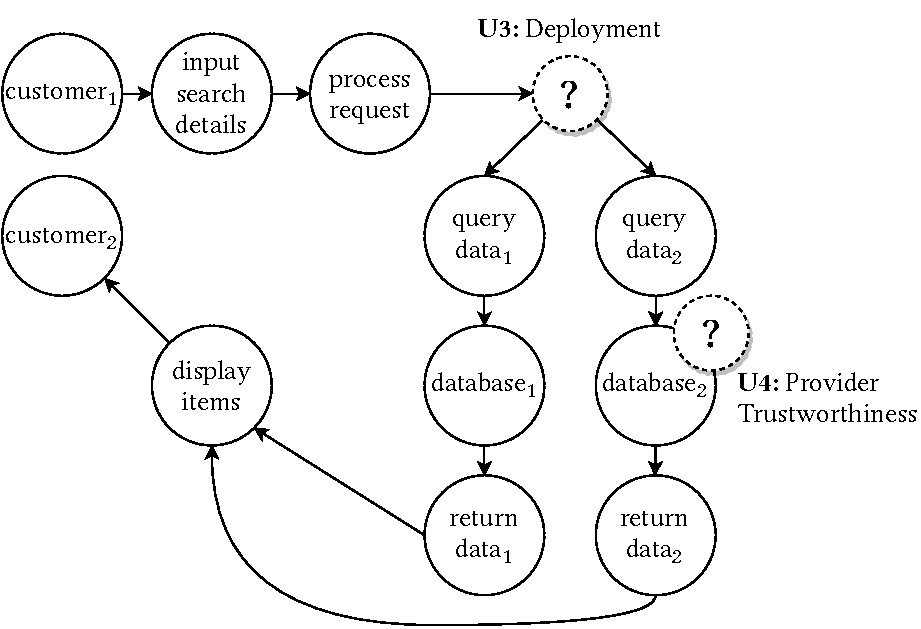
\includegraphics[width=0.85\textwidth]{figures/chapter5/onlineshop-dag.pdf}
    \caption{Data flow of the running example as \acf*{DAG} with annotated primary and secondary uncertainty, denoted by question marks.}
    \label{fig:classification:dag}
\end{figure}

\autoref{fig:classification:dag} shows the data flow of viewing available items from the running example, represented as \ac{DAG}.
We annotate the vertices and edges with primary and secondary uncertainty.
This example also illustrates how to transform a \ac{DFD} into a \ac{DAG}, as introduced in \autoref{sec:foundations:dfd}.
Cycles are replaced, e.g., the customer's sending and receiving activities are represented by separate vertices \cite{canfora_data_1992}.
The data flow of viewing available items is affected by two uncertainty sources: The uncertain deployment (\U{3}) and the provider's trustworthiness of the \emph{Cloud Service} (\U{4}).
The deployment (\U{3}) is classified as component uncertainty and thus falls into the group of \emph{secondary} uncertainty.
In this example, this affects the flow from the \emph{process request} vertex to the \emph{query data} vertices and all following vertices that represent the \emph{Database Service}.
The left flow from \emph{query data\textsubscript{1}} until \emph{return data\textsubscript{1}} represents the component being deployed on-premise, and the right flow represents the component being deployed in the cloud.
Here, we have to additionally consider the uncertainty about the provider's trustworthiness (\U{4}).
This uncertainty source is classified as external uncertainty and thus represents a \emph{primary} uncertainty.
For the sake of simplicity, we annotated this uncertainty only to the \emph{database\textsubscript{2}} vertex.

A \ac{DAG} $G = (V, E)$ consists of vertices $V$ and edges $E$.
Vertices affected by \emph{primary} uncertainty form a subset $V_{u} \subseteq V$.
We do not further restrict the size of $V_{u}$. 
The subset is empty if no primary uncertainty exists, but it can also contain every vertex of $V$.
In the running example, $V_{u} = \setted{\var{database_{2}}}$.
\emph{Secondary} uncertainty affects the edges of a \ac{DAG}.
Without limiting the generality, we can assume that the \ac{DAG} contains all known alternative scenarios, e.g., the deployment on-premise and in the cloud.
Then, each secondary uncertainty can be represented as a subset $E_{u_{i}} \subseteq E$.
All secondary uncertainties form a set $E_{u} = \setted{E_{u_{1}}, \dots, E_{u_{n}}}$ with size $\lvert E_{u} \rvert = n$.
Similarly, we do not further restrict its size but we require each edge to be contained at most once in a subset of a secondary uncertainty, i.e., $\forall e \in E, \forall i,j \in \setted{1, 2, \dots, n} : (e \in E_{u_{i}} \wedge i \neq j) \Rightarrow e \notin E_{u_{j}}$.
Otherwise, we would allow for the interference of secondary uncertainties.
In the running example, $E_{u_{1}} = \setted{\flow{process~request}{query~data_{1}}, \flow{process~request}{query~data_{2}}}$ and $E_{u} = \setted{E_{u_{1}}}$.

Already an example of this size demonstrates the benefits of including uncertainty as a first-class entity in the design \cite{garlan_software_2010}.
It helps to better understand the locations of uncertainty sources and even to investigate simple uncertainty interactions \cite{camara_uncertainty_2024}.
In this example, Uncertainty \U{4} is only relevant if the \emph{Cloud Service}, which is represented by the right data flow, is selected as deployment in Uncertainty \U{3}.
We consider this fact in the classification of the uncertainty sources in \autoref{sec:classification:runningexample}.
Here, we classify the impact of Uncertainty \U{3} as direct and the impact of Uncertainty \U{4} as indirect as it depends on another uncertainty, i.e., the Uncertainty \U{3}.
Representing uncertainty as primary and secondary uncertainty in \acp{DAG} visualizes such effects.
To this end, we actively manage a model with uncertainty instead of modifying the model to exclude uncertainty \cite{perez-palacin_dealing_2014}.

\finding{Including uncertainty sources as first-class entity in \acfp{DFD} simplifies their investigation, modeling, and analysis.
Even simple \ac{DFD} representations like \acfp{DAG} are sufficient to gain insights about the direct and indirect effects of uncertainty.
Here, we partition the five uncertainty types of the classification category \emph{Architectural Element Type} into two groups:
\emph{Primary} uncertainty directly affects vertices of \acp{DAG} while \emph{secondary} uncertainty affects edges between vertices.}





\section{Uncertainty Catalogs to Support the Identification}%
\label{sec:classification:identification}

Although classifying uncertainty is necessary to understand the differences in nature and type \cite{perez-palacin_uncertainties_2014}, it is not sufficient to enable the early identification of uncertainty sources.
Our classification shown in \autoref{sec:classification:classification} and also model-based confidentiality analyses require the uncertainty sources to be known to the software architect who conducts the assessment.
Uncertainty sources unknown to the architect, can neither be represented nor considered.
We motivated this \acf{UAP} already at the beginning of \autoref{ch:classification} and also in Problem \PR{1}{4}.

\begin{figure}
    \centering
    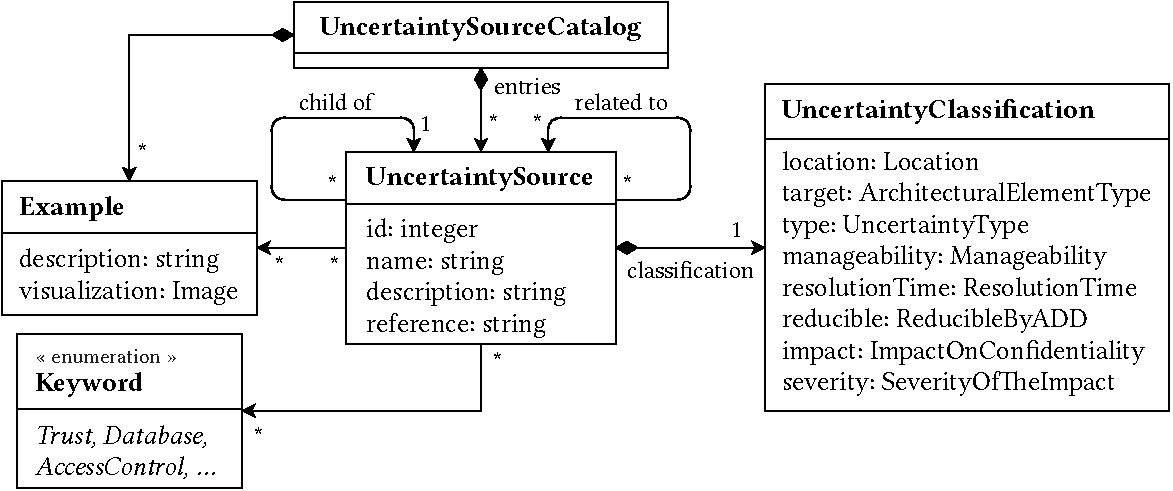
\includegraphics[width=\linewidth]{figures/chapter5/arc3n-metamodel.pdf}
    \caption[Simplified metamodel of the uncertainty source catalog.]{Simplified metamodel of the uncertainty source catalog. To simplify the illustration, we leave out all types of the UncertaintyClassification and refer to their comprehensive definition in \autoref{sec:classification:classification}.}
    \label{fig:classification:identification:metamodel}
\end{figure}

We propose a solution based on collecting and relating uncertainty sources and providing context information \cite{hahner_arcn_2024}.
\autoref{fig:classification:identification:metamodel} shows the metamodel of an \emph{Uncertainty Source Catalog}.
The \emph{Uncertainty Source Catalog} consists of \emph{Uncertainty Sources} and \emph{Examples} that demonstrate these sources.
Each source consists of a unique id, a name, a description, and a literature reference for additional information about its origin.
It can be related to an arbitrary number of other sources and can have children which represent inheritance between sources.
To classify the source, it is described by an \emph{Uncertainty Classification} using the categories of our classification \cite{hahner_classification_2023}, presented in \autoref{sec:classification:classification}.
Last, sources reference appropriate \emph{Examples} that consist of a description and a visualization.
\emph{Examples} can be used to explain more than one \emph{Uncertainty Source}, and a source can be illustrated with more than one example.
Last, \emph{Uncertainty Sources} can be further described by \emph{Keywords} to group uncertainty sources beyond their classification.

The \emph{Uncertainty Classification} represents the application of our classification to an uncertainty source, as exemplified in \autoref{sec:classification:runningexample}.
In our running example presented in \autoref{ch:runningexample}, Uncertainty \U{4} describes the unknown trustworthiness of the cloud service provider.
The \emph{Uncertainty Classification} shows the selected classification options, e.g., the location of the system environment, or the manageability of partially reducible, see \autoref{table:classification:example:two}.
Besides referencing the classification, the \emph{Uncertainty Source} has an id, a name, a description, and literature references for further information \cite{hahner_classification_2023,ramirez_taxonomy_2012}.
In our initial population of the catalog \cite{dataset}, we use the following example to explain the source: \enquote{In a cloud-based application, the uncertainty about the deployment provider's trustworthiness involves questioning whether the chosen cloud service ensures data security and system availability or whether or not data is made available to third parties such as governmental institutions.}
The \emph{Uncertainty Source} is tagged with the keyword \emph{Trust}.

\begin{figure}
    \centering
    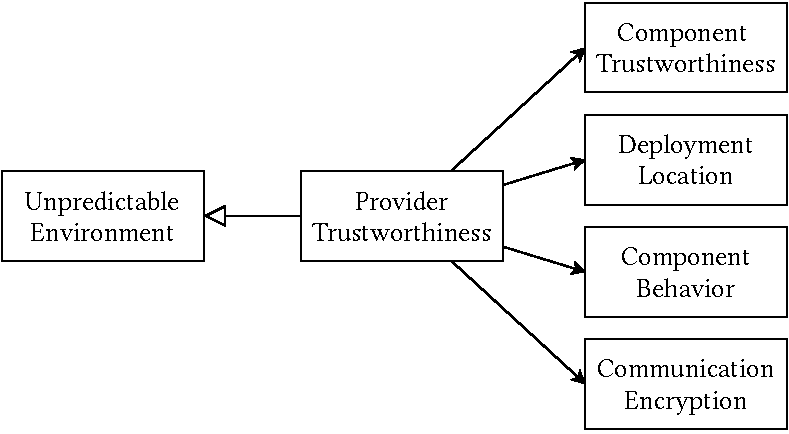
\includegraphics[width=0.8\linewidth]{figures/chapter5/arc3n-relations.pdf}
    \caption{Uncertainty source about the \enquote{Provider Trustworthiness} with its parent uncertainty source \enquote{Unpredictable Environment} and related uncertainties.}
    \label{fig:classification:identification:uncertaintygraph}
\end{figure}

In addition to its own properties, classification, examples, and keywords, \emph{Uncertainty Sources} can have relations and parent uncertainties.
In our example, \emph{Provider Trustworthiness} is a child of the uncertainty source \emph{Unpredictable Environment} \cite{ramirez_taxonomy_2012}, and related to uncertainty sources of our initial population regarding encrypted communication, component trustworthiness, and deployment location.
This is illustrated in \autoref{fig:classification:identification:uncertaintygraph}.

Combined, this information provides comprehensive context knowledge for software architects, raises awareness, and simplifies the assessment.
By attaching this information and also linking related uncertainty types, we address the organizational challenges of collecting uncertainty sources and enable to search and filter for uncertainty sources.
Additionally, there are no space limitations regarding examples, visualizations, and discussions.
To demonstrate this, we enriched 51 uncertainty sources from multiple classifications \cite{hahner_classification_2023,ramirez_taxonomy_2012} with context information, examples, and also uncertainty relations and inheritance as part of our data set \cite{dataset}.
In sum, this addresses Problem \PR{1}{4} and enables non-experts to reuse expert knowledge on uncertainty sources.

Note that the current state of research cannot create a generally applicable and comprehensive answer to identifying all possible uncertainty sources \cite{weyns_towards_2023}.
However, processing, persisting and relating information about uncertainty sources provides a pragmatic first step, especially for practitioners \cite{hahner_arcn_2024}.
To this end, approaches like this uncertainty source catalog are steps towards also addressing unanticipated changes that are not totally unforeseeable \cite{garlan_software_2010}.
Following the discussion about the orders of uncertainty \cite{armour_five_2000}, we hereby lower the order of uncertainty from the \emph{third} to the \emph{second} order. 
Although there can be a lack of awareness of an individual, we provide means to identify some uncertainty sources, which previously were unknown to this individual \cite{perez-palacin_uncertainties_2014}.

\finding{Knowledge about uncertainty sources can be reused across software architectures. 
Extending the classification of uncertainty sources with descriptions, examples, keywords, and relations between uncertainty sources helps in the identification and simplifies the assessment.
This reuse of expert knowledge addresses the \acf{UAP} and helps to deal with the ever-present challenge of unanticipated change.}





\section{A Collaborative Approach for Uncertainty Catalogs}%
\label{sec:classification:collaboration}

Our classification presented in \autoref{sec:classification:classification} provides the terminology to understand and discuss uncertainty sources, and the catalog meta model presented in \autoref{sec:classification:identification} simplifies the identification of relevant uncertainty sources and sharing of knowledge.
However, to be applicable, knowledge reuse must be simplified and should not be limited to individuals or institutions.
With Problem \PR{1}{5}, we stressed the importance of an open and publicly available catalog of uncertainty sources.
Collecting uncertainty sources only within publications \cite{ramirez_taxonomy_2012} or data sets \cite{hahner_classification_2023} lacks reusability, extensibility, and availability.
To address this, we propose a web-based catalog approach in the following.

\begin{figure}
    \centering
    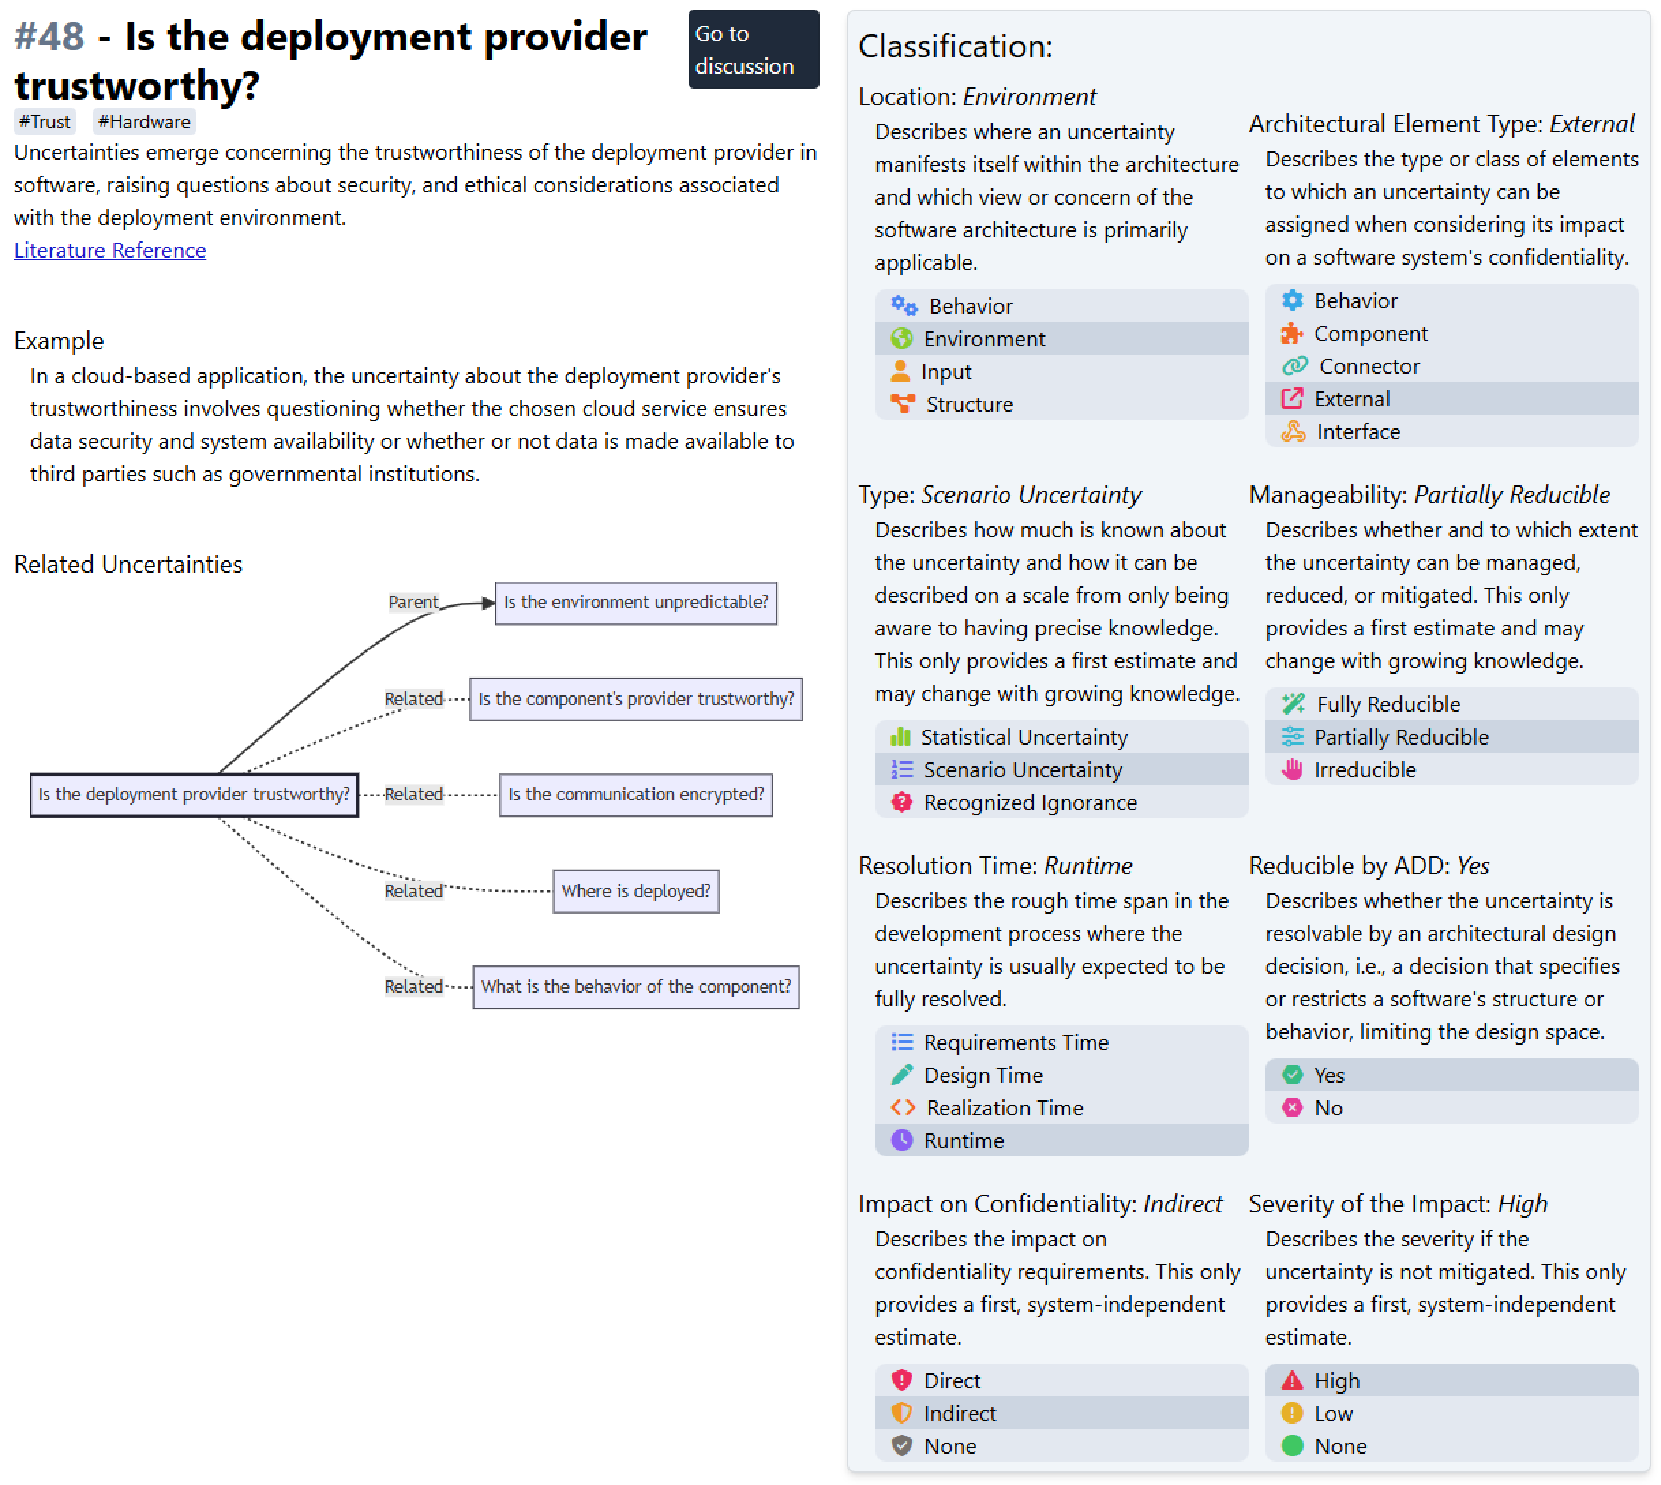
\includegraphics[width=\linewidth]{figures/chapter5/arc3n-screenshot.pdf}
    \caption[Screenshot of the detail view of our tooling.]{Screenshot of the detail view of our tooling \arcen. It shows the description, explanation, and classification of the uncertainty source regarding the trustworthiness of a resource provider.}
    \label{fig:classification:collaboration:screenshot}
\end{figure}

We realized our meta model and catalog approach as \textbf{\arcen}, which stands for \emph{Rese\textbf{arc}h \textbf{arc}hive for Software-\textbf{Arc}hitectural U\textbf{n}certainty}\footnote{\arcen is open-source and available online: \url{https://arc3n.abunai.dev/}. It is also archived in our data set \cite{dataset}. Any similarities by name with extensively praised jewels are completely coincidental.}.
Our tooling revolves around a table of uncertainty sources and their classification which allows for quick navigation, search, and filtering by keywords or classification categories.
By selecting a source, software architects can see its description, examples, related sources, and its classification.
Because there is no space limitation, the selected options of the classification can be explained in detail, as shown in \autoref{fig:classification:collaboration:screenshot}.
We also provide further explanation of all classification categories and relate known uncertainty sources similar to \autoref{fig:classification:identification:uncertaintygraph}.
Software architects can quickly navigate through uncertainty sources, examples, and classification.
Last, the full catalog can be downloaded in a machine-readable \ac{JSON} format.

All four uncertainty sources of our running example are contained in the initial population of our catalog.
Thus, security experts could become aware of these uncertainty sources by using our tool support.
To identify the uncertainty of the provider's trustworthiness (\U{4}), they could search for trust-related uncertainty sources or navigate to this uncertainty by its related uncertainty sources, e.g., the unpredictable environment or the encrypted communication.
They could even identify the uncertainty by investigating the open deployment decision with Uncertainty \U{3} as both uncertainty sources are related.

We chose a web-based approach to minimize the effort required to set up and use the tooling.
We use a GitHub \cite{GitHub2024} git repository as the backend for adding new uncertainty sources as well as discussions between participants.
New uncertainty sources can be added directly from within our tool support and are then retrieved by using the open GitHub API \cite{GitHub2024}.
This enables lightweight and openly accessible storage of all required information.
We choose GitHub to minimize the risk of link decay, which is especially prominent on institutional websites \cite{goh_link_2007}.
The information retrieval is automated using a DevOps pipeline based on GitHub Actions \cite{GitHub2024}.
Once the information has been updated, our tooling works completely autonomously and can be self-hosted or used locally.
This enables the easy integration of other information sources and also simplifies switching to other platforms like GitLab.

Our tooling \arcen collects uncertainty sources in a central place instead of relying only on publication-based collections which simplifies the collaboration of researchers and practitioners.
We foster two types of collaboration: \arcen benefits the communication between different roles with different knowledge, e.g., security experts and software architects. 
It also benefits peers with the same role as a shared catalog for exchange and documentation.
New uncertainty sources can be proposed by everyone based on the open-source GitHub repository.
All required information is stored as part of the tool support and can be downloaded in third-party analyses.
In sum, this approach provides an easy-to-use, extensible, and open collaborative approach to address Problem \PR{1}{5}.
Note that we do not claim comprehensiveness regarding uncertainty sources with this catalog.
We do also not claim long-term availability over decades.
Nevertheless, this approach is a proposal towards an open and available catalog to foster collaboration \cite{sterz_intelligente_2022}.





\section{Assumptions and Limitations}%
\label{sec:classification:limitations}

In this section, we discuss the assumptions and limitations of the identification and classification approaches presented in this chapter.
We partition these into five groups: The focus on confidentiality, the use of software architecture-based approaches at design time, the lack of automated analysis, the cooperation required for collaborative approaches, and the ever-present challenge of unanticipated change.

\paragraph{Focus on confidentiality}
First, we only focus on confidentiality as a central quality attribute of our classification.
While this reduces the generalizability, we do this intentionally to obtain more precise results for the modeling and analysis of uncertainty sources.
As demonstrated, the focus on confidentiality enables the connection of the uncertainty types to \acp{DFD}, which simplifies later data flow-based confidentiality analysis.
Additionally, we assume that the concepts can at least be applied partially to related quality attributes like integrity \cite{boltz_extensible_2024,seifermann_architectural_2022}.
Using the location as a central classification category and representing uncertainty in flow diagrams were the inspirations for other work \cite{acosta_uncertainty_2022,camara_uncertainty_2024}.
Nevertheless, we do not claim generalizability beyond confidentiality.

\paragraph{Using the software architectural abstraction}
Similarly, we limit ourselves to software-architectural uncertainty, as defined in \autoref{sec:classification:relation}.
This was also an explicit decision due to fit existing modeling \cite{reussner_modeling_2016,seifermann_unified_2021} and analysis \cite{seifermann_data-driven_2019,seifermann_detecting_2022,tuma_flaws_2019} approaches for confidentiality.
Still, most categories are general enough to be used even without explicit models, e.g., \emph{Type}, \emph{Manageability}, or \emph{Resolution Time}.
We assume that software architects and security experts already have enough knowledge about the software system to assess uncertainty at design time.
Such assumptions exist in many architecture-based analyses \cite{seifermann_architectural_2022,walter_context-based_2023}.

\paragraph{Transitive impact of uncertainty}
Third, the approaches for identification and classification provide no assistance for the transitive impact of uncertainty.
The uncertainty source is often not the location where the uncertainty affects confidentiality and where it can be mitigated.
We presented the relation of uncertainty sources and their impact in \autoref{sec:classification:relation}, e.g., with the transitive impact of the Uncertainty \U{1} about the user input to the \emph{Database Service} shown in \autoref{fig:classification:example}.
However, to face such propagation effects, a precise description of uncertainty---such as our classification---is required in the first place.
Additionally, the modeling and analysis of uncertainty for design-time confidentiality analysis require tool support as \enquote{detecting confidentiality issues manually is not feasible} \cite{seifermann_data-driven_2019}.
We will address this limitation in the following chapters.

\paragraph{Collaboration for joint uncertainty catalogs}
Our web-based approach \arcen represents a publicly available uncertainty catalog.
Here, we assume that researchers and practitioners alike benefit from sharing knowledge about uncertainty sources, as known from legal sciences \cite{sterz_intelligente_2022}. 
However, companies or institutions could try to keep the information private, especially regarding sensitive topics like security.
The lack of willingness to cooperate limits the benefits of a shared knowledge base.
Nevertheless, \arcen could also be used in a closed environment but with limited usefulness.

\paragraph{Unanticipated change}
We do not claim to have solved the challenge of unanticipated change.
A recently published research agenda \cite{weyns_towards_2023} names the challenge of end-to-end approaches that can operate in changing real-world conditions.
We do not provide a solution to such unanticipated change.
However, our identification approach represents a pragmatic approach towards reducing the effect to the individual by sharing knowledge about them, i.e., making them known.
In sum, our catalog approach can be seen as a first step or a potential part of a comprehensive solution.





\section{Summary and Outlook}%
\label{sec:classification:summary}

In this chapter, we presented our classification of \emph{software-architectural uncertainty} and our approach to address the identification of uncertainty.
This represents our first Contribution \C{1} and provides the answer to \RQ{1}.

First, we presented our understanding of the relation of uncertainty, confidentiality, and software architecture to address Problem \PR{1}{1}.
We highlighted the distinction between an uncertainty source and its impact.
The former represents the origin of uncertainty in the software system or its environment while the latter represents the actual location of the impact of the uncertainty source on confidentiality.
We also related the notion of uncertainty to the terminology known from \acfp{SAS} \cite{weyns_introduction_2020}, the \emph{cone of uncertainty} \cite{mcconnell_software_1998}, and \acfp{ADD} \cite{kruchten_ontology_2004,jansen_software_2005}.

Based on this discussion, we investigated existing uncertainty classifications \cite{walker_defining_2003,perez-palacin_uncertainties_2014,ramirez_taxonomy_2012,mahdavi-hezavehi_classification_2017,bures_capturing_2020} and defined our own classification tailored to the impact on confidentiality, thereby addressing Problem \PR{1}{2}.
Our classification contains 8 categories with a total of 27 options.
They classify uncertainty in categories like location, manageability, or resolution time.
The central category is the \emph{Architectural Element Type} as this category describes where to annotate an uncertainty source in architectural models.
Last, we illustrated the classification using our running example.

Building on this classification, we addressed Problem \PR{1}{3} of representing uncertainty as a first-class concern in \acp{DFD}.
Our first finding was that the five uncertainty types of the aforementioned classification match the model elements of \acp{DFD}.
We then partitioned the five uncertainty types category into \emph{primary} and \emph{secondary} uncertainty.
This enables a simple and straightforward representation of uncertainty in \acp{DAG}, which can be used to represent \acp{DFD}.
Primary uncertainty affects vertices, and secondary uncertainty affects edges between vertices.

Afterward, we extended the classification and presented a meta model for \emph{uncertainty source catalogs}, which addresses Problem \PR{1}{4}.
We proposed the enrichment of classified uncertainty sources with descriptions, keywords, and examples.
Additionally, uncertainty sources are usually not independent \cite{camara_addressing_2022} and thus can have relations and inheritance.
By collecting such information in a central archive, the \ac{UAP} can be partially addressed.

Last, we presented our tooling \arcen to create an open catalog of uncertainty sources and to address Problem \PR{1}{5}.
Our initial population contains 51 uncertainty sources with descriptions, examples, and relations.
It is publicly available under an open-source license and can help to identify relevant uncertainty sources that were previously unknown to security experts.
By combining classification and identification, we support the first two activities presented in \autoref{sec:overview:procedure}.

\RQ{1} asked about the identification, description, and classification of software-architectural uncertainty regarding confidentiality.
Our comprehensive answer to this question comprises the inspection of existing classifications and the definition of a novel classification regarding the impact of uncertainty on confidentiality.
We derive five uncertainty types that fit \acp{DFD}, which are often used to analyze confidentiality \cite{seifermann_unified_2021}.
By applying these uncertainty types to \acp{DAG}, we close the gap between uncertainty sources and confidentiality.
Furthermore, our classification provides the means to describe and discuss uncertainty.
By extending the classification to form tool-supported uncertainty source catalogs, we ultimately also address the question of description and identification.

The benefits of our Contribution \C{1} include precise terminology to discuss and understand uncertainty regarding confidentiality.
This supports both software architects and security experts in modeling and analyzing software-intensive systems.
As proposed in \autoref{ch:overview}, we do not require an additional \emph{uncertainty expert} role, as the required knowledge is contained in the classification and the uncertainty source catalog.
Here, our tooling \arcen presents a useful starting point.
By identifying and assessing uncertainty sources early, the reasoning and prioritization of \acp{ADD} is simplified and costly backtracking is minimized.
This is especially true regarding uncertainty interactions \cite{camara_addressing_2022}, which represent uncertainty impacts that are particularly hard to find and mitigate.
Last, our classification lays the foundations for further integration of software-architectural uncertainty in the architecture-based analysis of confidentiality.

We will revisit the idea of representing uncertainty sources and their impact as first-class entities in \acp{DFD} and \acp{DAG} in the following chapters.
In \readingpath{ch:impactanalysis}, we discuss uncertainty propagation in architectural models and \acp{DFD} alike.
This will help to better understand the actual impact of uncertainty sources on confidentiality beyond the early assessment using our classification.
This also addresses the limitation of the sole classification regarding the transitive impact of uncertainty.
It also defines the foundations for later uncertainty-aware analysis in \readingpath{ch:confidentialityanalysis}.
Here, we will also see again the distinction between primary and secondary uncertainty and how it can be used to speed up data flow analysis.
Last, the evaluation of this chapter will be presented in \readingpath{ch:evaluation}.





\section{In Simpler Words}%
\label{sec:classification:simple}

In this chapter, we focus on two things: The classification and the identification of uncertainty.
This is an important first step because we first need to better understand the threat to confidentiality, which is uncertainty.
We define clear terms for software architects and security experts in the form of a classification.
Afterward, we show how to extend this classification in order to identify more uncertainty sources.

A classification helps to understand important properties of a classified element---in our case, uncertainty.
Many researchers already defined many classifications of uncertainty.
However, they do not fit our purpose, relating uncertainty to confidentiality.
Thus, we define our own classification based on the existing ones.
We propose different categories like the location, the manageability, or the severity of the impact.
For instance, the uncertainty regarding user behavior can be located in the system input as users operate a software system.
We cannot control their input but we can try to think of possible behavior in advance and thus partially reduce this uncertainty.
If the user behaves maliciously and tries to attack our system, the severity of the impact can be high.
In total, we define eight categories like these three.
They help us to better understand uncertainty, and group uncertainty sources together.
We apply this knowledge to data flow diagrams, a diagram type that is often used to reason about confidentiality.
By connecting this uncertainty terminology to data flow diagrams, we lay the foundations for the automated analyses we will present in the following chapters.

To help software architects and security experts even more, we also discuss how to identify uncertainty sources.
If you had not read the previous paragraph, you might not have known about the uncertainty of the user's behavior.
This is the nature of unexpected changes---often, you do not even know that you do not know about the change.
But now that I told you, you know about the uncertainty of user behavior.
You still do not know how the user will behave in the end, but you are at least aware of the issue.
We present a software tool that helps to collect uncertainty sources and make software architects and security experts aware of them.
This also helps to connect different uncertainty sources, as they often have relations.
For instance, if we apply input validation to address the uncertain user input, we can address this uncertainty.
But if we do not know how this input validation works and whether it always works correctly, the validation itself is an uncertainty source.
Then, both uncertainties are connected---this is called \emph{uncertainty interaction}.
Uncertainty interactions are particularly dangerous and hard to find.
Our contribution regarding the identification and classification can also help here.

\chapter{Uncertainty Propagation to Enable Uncertainty Impact Analysis}%
\label{ch:impactanalysis}%


In this chapter, we present the second Contribution \C{2}.
This contribution covers the third activity shown in \autoref{sec:overview:procedure}, i.e., the propagation of uncertainty.
We present means to model and analyze uncertainty in software architectures in order to enable the early assessment of the potential impact of uncertainty on confidentiality.

As motivated throughout this thesis, uncertainty can quickly become critical, especially regarding security-related properties like confidentiality.
For proactive decision-making as implied by \emph{Privacy by Design} \cite{schaar_privacy_2010} and adaptation to a changing environment, uncertainty should be analyzed as early as possible.
This requires means to model and analyze uncertainty that build on existing \acfp{ADL} and do not require extensive knowledge or modeling and analysis effort.
As implied by the term \emph{what-if} analysis, we aim to quickly understand the potential impacts of uncertainty without having to re-model---or even worse, re-implement---a software system.

Much is yet unknown about potential uncertainty sources and their effects \cite{hahner_dealing_2021}, e.g., in early design due to abstract requirements and open decisions \cite{mcconnell_software_1998}, or in systems of systems because of unpredictable behavior and complex dependencies and interactions \cite{oquendo_coping_2019,camara_addressing_2022}.
Here, uncertainty in a software system (e.g., component choices) or its environment (e.g., user input) can void assumptions \cite{acosta_uncertainty_2022}.
Design time confidentiality analysis can help to identify potential confidentiality violations early \cite{seifermann_detecting_2022}, but is either not suited to deal with uncertainty \cite{seifermann_architectural_2022}, or requires to much additional modeling effort \cite{boltz_handling_2022, walter_architectural_2022}.
This lack is supported by the literature.
\textcite{hezavehi_uncertainty_2021} recently found a \enquote{lack of systematic approaches for managing uncertainty} \cite{hezavehi_uncertainty_2021}.
This also becomes visible in a recent study by Troya et al.~\cite{troya_uncertainty_2021}, which highlights the opportunity of providing useful notations and tool support to model and analyze uncertainty.

We aim to address this problem with a tool-supported approach for \emph{Uncertainty Impact Analysis} regarding confidentiality.
Based on software-architectural modeling, we propagate uncertainty sources through the software system to identify impact locations that subsequently can be analyzed and mitigated accordingly.
This approach fills the gap between identifying uncertainty sources and understanding their actual impact on a system's confidentiality by using the information of the software's architecture.
This also addresses the limitation of understanding the transitive impact of uncertainty described in \autoref{sec:classification:limitations}.
To achieve this, we build upon the concept of architecture-based change impact analysis \cite{heinrich_methodology_2018,rostami_architecture-based_2015,rostami_architecture-based_2017}.
Such analyses trace changes, e.g., replacing components or altering interfaces, and predict the impact on the software system.
To analyze the impact of uncertainty on confidentiality, we combine this structural propagation with the propagation along extracted data flows.
This enhances the precision of the impact, especially regarding confidentiality, as \enquote{problems tend to follow the data flow, not the control flow} \cite{shostack_threat_2014}.
By calculating the impact of uncertainty, software architects can identify potential issues without laborious modeling and analysis of architectural variations \cite{hahner_model-based_2023,walter_architecture-based_2023}.

As defined in \autoref{sec:classification:relation}, we stress the importance of distinguishing an uncertainty \emph{source} and its \emph{impact}.
Only considering uncertainty sources rather than their impact impedes precise mitigation.
Moreover, similarly to confidentiality analysis \cite{seifermann_data-driven_2019}, manual propagation of uncertainty is not feasible, especially in large systems of systems.
Thus, the provided concepts need tool-supported modeling and analysis to aid software architects.
Here, we build on the classification of uncertainty, which was presented in the previous chapter, see \autoref{ch:classification}.
We summarize this research concern of uncertainty propagation and impact analysis in the second research question:

\RQtwo

We also present one extension to this work.
As acknowledged in \autoref{sec:classification:dfd}, sources of uncertainty are rarely independent, and their interactions can affect the overall system in subtle and unpredictable ways \cite{camara_uncertainty_2022}.
Similarly to the discussion presented in \autoref{ch:classification}, this \acf{UIP} demands representing uncertainty as a first-class concern.
To consider heterogeneous uncertainty sources, i.e., uncertainty which differs in representation and nature, and their propagation and interaction, we generalize the propagation concept to define \acfp{UFD} \cite{camara_uncertainty_2024}.
Building on our findings on \acfp{DFD} and uncertainty propagation presented throughout this thesis, we present an initial, yet more general approach to propagate uncertainty that is not limited to confidentiality.
This extension positions our work in the research area of \acfp{SAS} \cite{weyns_towards_2023} and shows further application possibilities.

The remainder of this chapter is structured as follows:
First, we present the problem statement.
We discuss how to represent uncertainty in architectural models using the \ac{ADL} \acf{PCM} \cite{reussner_modeling_2016}.
Afterward, we present uncertainty propagation separately for architectural models and \acp{DFD} and then combine these findings to define a joint uncertainty impact analysis regarding confidentiality.
Building on that, we combine the analysis with the identification approach presented in \autoref{sec:classification:identification}, to address the \acf{UAP} of uncertainty impact analysis.
Last, we generalize the propagation concept to define \acp{UFD}.
We close the chapter with a discussion of assumptions and limitations and give a summary and an outlook.

\ownpublications{
\fancycite{acosta_uncertainty_2022},
\fancycite{hahner_architecture-based_2023},
\fancycite{camara_uncertainty_2024},
\fancycite{hahner_arcn_2024}
}





\section{Problem Statement}%
\label{sec:impactanalysis:problem}

We summarize the problems \textbf{P1} -- \textbf{P4} addressed by Contribution \C{2}.
Finding solutions to these problems helps to provide a comprehensive answer to \RQ{2}.

\paragraph{P1: Representation of uncertainty in architectural models}\label{p:2:1}
In order to consider uncertainty in software architecture, we require means to describe uncertainty in the architectural abstraction.
We benefit from the restriction to software-architectural uncertainty of our classification \cite{hahner_architecture-based_2023} that can be used as a baseline.
Nevertheless, we need to relate the different uncertainty types to elements of the software architecture \cite{troya_uncertainty_2021}.
The representation of uncertainty in architectural models can be realized by annotating uncertainty to \acp{ADL} like the \ac{PCM} \cite{reussner_modeling_2016}.
Last, we need to understand the representation of the impact of uncertainty both in \ac{PCM} and \acp{DFD}.

\paragraph{P2: Propagation of uncertainty for uncertainty impact analysis}\label{p:2:2}
We require rules to propagate uncertainty in all models that are considered in design time confidentiality analysis.
This includes architectural models described with \acp{ADL} and also \acp{DFD}.
For both representations, we need to understand how uncertainty can impact confidentiality, and how this impact can be calculated.
We also need to relate both representations to define a comprehensive uncertainty impact analysis.
Last, analysis automatization is required as manually propagating uncertainty in large software systems is not feasible.

\paragraph{P3: Identifying uncertainty for uncertainty impact analysis}\label{p:2:3}
Similar to other architecture-based analyses under uncertainty \cite{hahner_model-based_2023,walter_architectural_2022}, uncertainty impact analysis suffers from the \acf{UAP}.
We cannot assume that software architects are aware of all relevant uncertainty sources.
We can also not assume that software architects have enough expertise to annotate the correct uncertainty sources in the architectural model.
These shortcomings severely limit the accuracy of the uncertainty impact analysis as only identified and correctly annotated uncertainty sources can be propagated.
Addressing this problem also helps to move towards end-to-end approaches \cite{weyns_towards_2023}.

\paragraph{P4: Uncertainty propagation to address uncertainty interactions}\label{p:2:4}
The \acf{UIP} can be addressed using uncertainty propagation.
This requires appropriate notations to follow the flow of uncertainty in software systems.
These notations need to support not only homogeneous uncertainty but also heterogeneous uncertainty of different type and nature.
Another key requirement for such a notation is that it should be able to capture how uncertainty propagates both horizontally, i.e., within the same level of abstraction, and vertically, i.e., across different levels of abstraction \cite{camara_addressing_2022}.




\section{Representing Uncertainty in Architectural Models}%
\label{sec:impactanalysis:representing}

In order to enable architecture-based uncertainty impact analysis regarding confidentiality, we first need to understand the representation of uncertainty sources and their impact both in architectural models and \acp{DFD}.
Here, we build on the findings presented in \autoref{sec:classification:dfd} about representing uncertainty sources in \acp{DFD} and \acfp{DAG}.
In this section, we discuss the relation of software architectural models and \acp{DFD} and the role of uncertainty in both representations of a software system.
Afterward, we define a meta model for representing the propagated uncertainty impact in \acp{DFD} and derive which elements of a software architecture can be annotated with uncertainty sources.
We build on the \ac{PCM} as it represents a mature and widely-used \ac{ADL}.
Nevertheless, the findings of this section are also applicable to other representations of a software architecture like \acf{UML} diagrams \cite{object_management_group_unified_2015}.
This addresses our first Problem \PR{2}{1} about the representation of uncertainty in architectural models.


\subsection{Modeling Uncertainty Sources and Uncertainty Impacts}

\begin{figure}
    \centering
    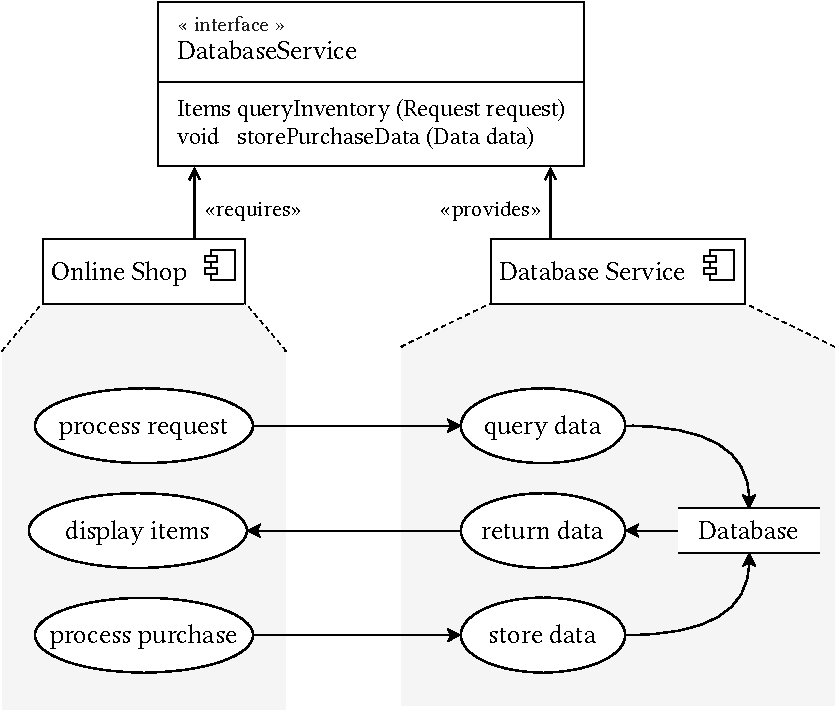
\includegraphics[width=0.8\linewidth]{figures/chapter6/mapping-example.pdf}
    \caption{Simplified mapping of the components of the running example to a \acf*{DFD}.}
    \label{fig:impactanalysis:representing:example}
\end{figure}

We start by explaining the relation of a high-level structural view like a \ac{PCM} component repository model and \acp{DFD} using our running example.
\autoref{fig:impactanalysis:representing:example} shows the simplified mapping of the two components \emph{Online Shop} and \emph{Database Service}, the interface that connects those components, and a \ac{DFD} showing the data flows of querying and purchasing items.
This mapping has been precisely defined by \textcite{seifermann_architectural_2022}, which includes the automated extraction of \acp{DFD} from the \ac{PCM}.

The components of \autoref{fig:impactanalysis:representing:example} are connected by an interface and additionally encapsulate their own behavior.
A \ac{PCM} component can have multiple intended purposes, e.g., the \emph{Online Shop} component is used to process item requests and to process purchases.
This is represented in the signatures of an interface and also becomes visible when looking at the \ac{DFD}.
Additionally, a single interface signature's behavior can be represented by multiple \ac{DFD} nodes, e.g., querying items with the signature \emph{queryInventory} involves the \emph{query data}, \emph{Database}, and \emph{return data} nodes.
Last, some information of the architectural model is not mapped to \acp{DFD}, e.g., every information related to the details of signatures and interfaces.
We find that there is no one-to-one mapping between an architectural model of the \ac{PCM} and a \ac{DFD}.
Both models can represent the same software system but show different concerns and abstraction levels.

When we discussed the difference of uncertainty \emph{sources} and the \emph{impact} of uncertainty on confidentiality, we stated that the locations can differ.
\autoref{fig:classification:example} showed an uncertainty source annotated to the customer using the \emph{Online Shop} and its potential impact to the \emph{Database Service}.
This relation also becomes visible in this mapping, illustrated in \autoref{fig:impactanalysis:representing:example}.
An uncertainty source in the input of the \emph{process request} node could affect the \emph{query data} node and transitively affect all other nodes in the flow, starting with the \emph{Database}.
Put simply, unspecified user input could lead to confidentiality violations in all of these nodes.
We find that a single uncertainty source can impact multiple nodes of a \ac{DFD} and that the representation of \acp{DFD} is suited to express this impact.

\begin{figure}
    \centering
    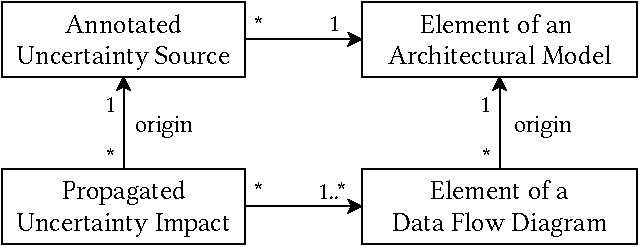
\includegraphics[width=0.65\linewidth]{figures/chapter6/relation-source-impact.pdf}
    \caption{Simplified view on the relation of software-architectural uncertainty sources, their propagated impact, software architectural models, and \acfp*{DFD}.}
    \label{fig:impactanalysis:representing:relation}
\end{figure}

These findings are summarized in \autoref{fig:impactanalysis:representing:relation}.
An element from the architectural model can be represented by zero, one, or many elements of \ac{DFD}.
Our example shows all three cases, as discussed previously.
When extracting \acp{DFD} from \ac{PCM} with the mapping of \textcite{seifermann_architectural_2022}, every \ac{DFD} element can be traced back to one originating element of the software architecture.

Software architects annotate identified uncertainty sources to the architectural model as this enables them to stay on the architectural abstraction \cite{hahner_architectural_2021}.
Although every uncertainty source is annotated to exactly one element of the software architecture, there is no limit how many uncertainty sources can be annotated to a single element.
Furthermore, there also can be elements without any annotated uncertainty, either because it has not yet been identified, or because it is currently not relevant.
See the procedure of uncertainty-aware analysis described in \autoref{sec:overview:procedure} for more details.

As shown in the discussion in \autoref{fig:impactanalysis:representing:example}, a single annotated uncertainty source can have multiple impact locations.
Similarly to the relation of architectural elements and \ac{DFD} elements, every impact can be traced back to one originating uncertainty source.
Put simply, once the confidentiality has been violated, software architects can trace the violation back to its cause, e.g., an overlooked uncertainty source.
A propagated uncertainty impact affects at least one \ac{DFD} element---or more, as seen in the running example.
Nevertheless, not every element of a \ac{DFD} has to be impacted by uncertainty.

This relation of uncertainty sources, their propagated impact, architectural models, and \acp{DFD} lays the foundation for all further discussions in this chapter.
Note that this is only one view on the relation of these concepts.
For instance, one could argue that a single uncertainty source can affect multiple elements of an architectural model\footnote{When I came back from SEAMS '23 in Australia where I presented this work, I had this very discussion with Shmuel Tyszberowicz. I conclude that allowing one uncertainty source to only affect a single element does not limit the generality as there could be infinite uncertainty sources that affect different elements and that are related and analyzed together.}.
For the sake of consistency, we are keeping this view for the remainder of this chapter. 

\finding{Architectural models are a suitable representation to be annotated with software-architectural uncertainty sources and \acfp{DFD} are suitable to represent their impact on confidentiality.
Multiple \ac{DFD} elements can represent a single element of the architectural model, and similarly, multiple elements of a \ac{DFD} can be impacted by a single uncertainty source.}


\subsection{A Meta Model of the Uncertainty Impact in Data Flow Diagrams}

In \autoref{sec:classification:classification}, we defined our classification of uncertainty that is tailored to confidentiality.
The category \emph{Architectural Element Type} is used as the primary category for annotating architectural models.
It offers five uncertainty types, i.e., five possible target elements of uncertainty.
Component uncertainty represents uncertainty in software components, connector uncertainty represents uncertainty in the wiring between components, interface uncertainty represents uncertainty in interfaces, external uncertainty represents uncertainty in resources, or users, and behavior uncertainty represents uncertainty in behavior descriptions.
See \autoref{table:classification:classification:architecturalelementtype} for details on the classification and \autoref{table:classification:mapping} for details on the relation of these options and \ac{DFD} elements.
We do not limit our modeling to a certain type of uncertainty, e.g., environmental uncertainty \cite{boltz_handling_2022}, or structural uncertainty \cite{walter_architectural_2022} in the following, but aim to support all five uncertainty types.

While these uncertainty types and their associated software-architectural elements are sufficient to document uncertainty sources, additional effort is required to also represent their impact, see \autoref{fig:impactanalysis:representing:relation}.
As discussed, confidentiality and the impact of uncertainty on confidentiality is best investigated using \acp{DFD}.
To this end, we extend the unified modeling primitives of \acp{DFD} \cite{seifermann_unified_2021}, which were introduced in \autoref{sec:foundations:dfd} and related to uncertainty in \autoref{sec:classification:dfd}.

\begin{figure}
    \centering
    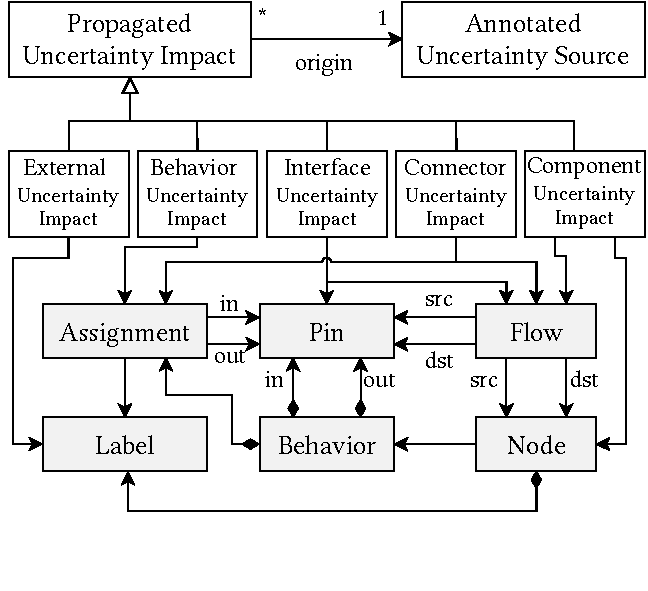
\includegraphics[width=0.7\linewidth]{figures/chapter6/metamodel-uia.pdf}
    \caption{Meta model of \acfp*{DFD} with the five different uncertainty impact types.}
    \label{fig:impactanalysis:representing:metamodel}
\end{figure}

\autoref{fig:impactanalysis:representing:metamodel} shows our meta model that combines the \ac{DFD} primitives (highlighted gray) and the five uncertainty types.
We extend the relation of uncertainty sources and their propagated impact to \ac{DFD} elements introduced in \autoref{fig:impactanalysis:representing:relation} based on the mapping shown in \autoref{table:classification:mapping}.
One \emph{Annotated Uncertainty Source} can have any number of \ac{DFD} elements affected by the \emph{Propagated Uncertainty Impact}.
We explain the relation of the five different uncertainty impact types and \ac{DFD} elements in the following.

\emph{Nodes} represent the system's structure and are affected by \emph{Component} uncertainty, e.g., Uncertainty \U{3} regarding the deployment of the \emph{Database Service} component in the running example would affect all nodes that represent this component.
We exemplified how to represent this in \acp{DAG} in \autoref{fig:classification:dag}.
\emph{Flows} connect these nodes by transmitting data and are affected by \emph{Connector Uncertainty}.
Additionally, \emph{Connector} uncertainty affects \emph{Assignments} of confidentiality-related labels, e.g., whether the user input is erroneous or malicious in Uncertainty \U{1} of the running example.
\emph{Flows} are also affected by \emph{Component} uncertainty, as altering components can change the flow of data, and also by \emph{Interface} uncertainty.
Primarily, \emph{Interface} uncertainty affects \emph{Pins} that decouple flows from a node and function as interfaces in the unified modeling primitives for \acp{DFD} \cite{seifermann_unified_2021}.
In \autoref{sec:classification:dfd}, we called these three uncertainty types \emph{secondary} uncertainty.
Also, in this meta model, we can see their broad impact on \ac{DFD} elements.
All \emph{secondary} uncertainty affects two different \ac{DFD} elements and can have a structural impact on the overall system.

In comparison, \emph{primary} uncertainty, i.e., \emph{Behavior} uncertainty and \emph{External} uncertainty, only affects one \ac{DFD} element.
Although this impact is more direct, we cannot make any claims on the severity or probability of confidentiality violations due to such uncertainty compared to \emph{secondary} uncertainty---this depends on the software system, the environment, and the uncertainty sources in both.
\emph{Behavior} uncertainty impacts the assignments that are used to represent the behavior of a \emph{Node}.
In our running example, Uncertainty \U{2} about the data processing could be represented as such an uncertainty source.
This would affect whether the behavior of the data processing node assigns the \emph{Labels} for validation or encryption.
Ultimately, this can lead to confidentiality violations similarly as all other uncertainty sources.
Last, \emph{Nodes} can also be described by \emph{Labels} to represent their confidentiality-related properties, which are affected by \emph{External} uncertainty.
In our running example, Uncertainty \U{4} can be represented as \emph{External} uncertainty affecting a label that expresses the trustworthiness of said \ac{DFD} node.

Our metamodel and its graphical representation in \autoref{fig:impactanalysis:representing:metamodel} demonstrate again the good fit of the five uncertainty types introduced by the category \emph{Architectural Element Type} of our classification to \acp{DFD}.
Every uncertainty impact affects another element type of the unified modeling primitives.
Additionally, all \emph{secondary} uncertainty types affect the flow, as discussed in \autoref{sec:classification:dfd}.
The only exception to this rule is the \emph{Behavior}, which has no associated uncertainty type because it only acts as a container for pins and assignments.
In sum, this meta model enables us to connect the uncertainty types from the software architecture to their corresponding impact type.
The representation based on \ac{DFD} elements simplifies the subsequent task of uncertainty propagation.

\finding{The propagated uncertainty impact can be represented by the five uncertainty types of the classification category \emph{Architectural Element Type}.
There is a direct relation of these types to the unified modeling primitives of \acfp{DFD}, which lays the foundation for the precise impact of uncertainty regarding confidentiality in software architectures.}


\subsection{Annotating Uncertainty Sources in the Palladio Component Model}

By now, we have discussed the relation of annotated uncertainty \emph{sources} and their propagated \emph{impact} with the more abstract view of architectural models and the more concrete view of \acp{DFD}.
However, to be applicable, one piece of the puzzle introduced in \autoref{fig:impactanalysis:representing:relation} is missing: The mapping of uncertainty sources to concrete elements of the architectural model.
Instead of only referring to architectural concepts like components, connectors, and interfaces, we discuss concrete annotation targets based on the \ac{ADL} \ac{PCM} \cite{reussner_modeling_2016} in the following.
These annotation targets can be derived by following the transformation \cite{seifermann_architectural_2022} from \ac{PCM} to \acp{DFD}.
Put simply, we investigate, which elements of the \ac{PCM} are relevant for \acp{DFD}---and thus, for confidentiality---and annotate uncertainty sources to them.
This not only concludes the relation discussed in this section but also lays the foundation for tool-supported modeling and automated analysis presented hereafter.

For the remainder of this chapter, we use the terminology known from the \ac{PCM}.
See \autoref{sec:foundations:architecture} for an overview of \ac{PCM}, or look into its comprehensive documentation \cite{reussner_modeling_2016,becker_palladio_2009,reussner_palladio_2011}.
To minimize confusion, we use the original terminology \cite{reussner_palladio_2011,reussner_modeling_2016} although there are slight deviations in the current Palladio implementation \cite{reussner_palladio_2024}.
However, this does only affect two \ac{PCM} element types used in the following: \emph{Signature} compared to \emph{OperationSignature}, and \emph{Interface} compared to \emph{OperationInterface}.
Note that there are also slight differences between the \ac{PCM} elements used for uncertainty impact analysis and those used to analyze confidentiality under uncertainty in later chapters because we only \emph{annotate} uncertainty source instead of altering the architectural model.
However, this is for purely pragmatic reasons that do not affect the underlying concepts.

\begin{table}
    \centering
    \begin{tabularx}{\linewidth}{lX}
        \toprule
        Uncertainty Type \,         & \ac{PCM} elements that can be annotated \\
        \midrule
        Component          & AssemblyContext \\
        Connector        & AssemblyConnector, ProvidedDelegationConnector \\
        Interface          & Signature, Interface \\
        External            & ResourceContainer, UsageScenario \\
        Behavior          & ExternalCallAction, EntryLevelSystemCall, SetVariableAction, BranchAction \\
        \bottomrule
    \end{tabularx}
    \caption{Mapping of the five uncertainty types to \acf*{PCM} elements.}%
    \label{table:impactanalysis:pcmmapping}
\end{table}

\autoref{table:impactanalysis:pcmmapping} shows the mapping of the uncertainty types to elements of the \ac{PCM} that can be annotated with this uncertainty source.
\emph{Component} uncertainty sources affect instances of components and are annotated to the \emph{AssemblyContext}.
\emph{AssemblyContexts} refer to component types from the \ac{PCM} component repository model and instantiate them within the concrete wiring of the \ac{PCM} system model.
Put simply, they represent concrete components and not component types and are thus suited to represent \emph{Component} uncertainty sources visible to software architects.
In our running example, we have two repository components, \emph{Online Shop} and \emph{Database Service}, which are both instantiated once.
To express uncertainty sources on type level, refer to \emph{Interface} uncertainty which annotates elements from the \ac{PCM} component repository model.

\emph{Connector} uncertainty affects inter-component structures, i.e., the wiring visible in the \ac{PCM} system model by using \emph{AssemblyConnectors}.
These connectors link concrete component instances, i.e., \emph{AssemblyContexts}, together.
In our running example, the connection of the \emph{Online Shop} and the \emph{Database Service} component is realized using such connectors.
Additionally, \emph{Connector} uncertainty can also affect \emph{ProvidedDelegationConnectors}.
These connectors represent system interfaces that can be used by users outside of the modeled system, e.g., in \emph{UsageScenarios}.
We support both connector types because both can be used to impact the usage of components, which is expressed by \emph{Connector} uncertainty.

\emph{Interface} uncertainty affects the interfaces that are defined in the \ac{PCM} component repository model.
Here, we support two levels of granularity: Either a single \emph{Signature} of an interface or the complete \emph{Interface}, i.e., all of its signatures, can be affected.
This enables software architects to minimize the annotation effort, e.g., to express that every communication over a selected interface is subject to uncertainty.
Note that in contrast to the first two uncertainty types, \emph{Interface} uncertainty is specified on a type level and not in the \ac{PCM} system model.
In our running example, the two components offer interfaces with multiple signatures.
One of these interfaces is illustrated in \autoref{fig:impactanalysis:representing:example}.

\emph{External} uncertainty affects the context of a software system, e.g., resources, and users.
It can be annotated to \emph{ResourceContainers}, which are part of the \ac{PCM} resource environment model, and \emph{UsageScenarios}, which are part of the \ac{PCM} usage model.
Both elements are part of the system environment and both can transitively affect the software system, e.g., because components are deployed to uncertainty-afflicted resources in the \ac{PCM} component allocation model.
Selecting these two elements to express environmental concerns that can affect confidentiality is inspired by architecture-based confidentiality analysis \cite{seifermann_data-driven_2019}.
In our running example, the \emph{On Premise Server} and the \emph{Cloud Service} represent \emph{ResourceContainers}.
The \emph{Customer} has multiple \emph{UsageScenarios}, e.g., browsing for items, or purchasing items.

\emph{Behavior} uncertainty affects the behavior of the software system and its users.
The behavior of the system is described in the form of \acfp{SEFF} in a \ac{PCM} component repository model.
Here, uncertainty can be annotated to \emph{ExternalCallActions} that represent components calling each other, \emph{SetVariableActions} that represent internal activities, and \emph{BranchActions} that can change the control flow.
All of these elements can affect the confidentiality of data flowing through them and are thus relevant for \emph{Behavior} uncertainty.
Last, \emph{Behavior} uncertainty can also be annotated in \emph{EntryLevelSystemCalls} that represent the user calling the system interface and are located in the \ac{PCM} usage model.
Although the location of classified uncertainty differs, i.e., uncertainty in the \emph{System Input} instead of the \emph{System Behavior}, the \emph{Architectural Element Type} option stays the same for impact analysis.
In our running example, the \emph{Customer} requesting the purchase of an item is represented by an \emph{EntryLevelSystemCall}, the storing of data called from the \emph{Online Shop} is realized with an \emph{ExternalCallAction}, and the data processing can be modeled with a \emph{SetVariableActions}.
For the sake of simplicity, we do not include branches.

In sum, all five types of uncertainty sources can be annotated to \ac{PCM} elements.
Based on the Palladio \cite{reussner_palladio_2024} tool support, existing modeling tools can be extended to support these annotations.
While uncertainty sources are best represented in the architectural model, their corresponding impact types are best represented in \acp{DFD}.
The uncertainty types of the category \emph{Architectural Element Type} originate from investigating existing classifications and \ac{DFD} notations.
Note that while these are generally applicable, alternative annotation targets other than the presented \ac{PCM} elements are possible \cite{benkler_architecture-based_2022}.
This is due to the nature of models representing reality, i.e., \ac{PCM} modeling software architecture \cite{stachowiak_allgemeine_1973}.

\finding{The source of the five uncertainty types of the category \emph{Architectural Element Type} can be annotated to the \acf{PCM}.
This \acf{ADL} can be extended to annotate uncertainty within the software system, e.g., its structure and behavior, and the system environment, e.g. usage scenarios and hardware resources.
Relating the five uncertainty types to concrete \ac{PCM} elements enables software architects to represent uncertainty sources on architectural abstraction.}





\section{Uncertainty Impact Analysis for Architectural Models}%
\label{sec:impactanalysis:pcmpropagation}

Building on the representation of uncertainty sources within architectural models, we can propagate the uncertainty to better understand its impact.
Starting from the annotation targets discussed in the previous section, we calculate this impact to define an \emph{uncertainty impact analysis} \cite{hezavehi_uncertainty_2021}.
Regarding confidentiality, this analysis requires two steps \cite{hahner_architecture-based_2023}.
First, the propagation within the architectural model, and second, the propagation in extracted \ac{DFD}.
As the uncertainty sources are annotated within the architectural model, we start with this part of the impact analysis.
As introduced previously, we will use the \ac{ADL} \ac{PCM} to detail the propagation rules.
This addresses Problem \PR{2}{2}.


\subsection{Adapting Change Impact Analysis to Uncertainty Propagation}

The name \enquote{uncertainty impact analysis} is inspired by architecture-based \emph{change impact analysis} \cite{heinrich_methodology_2018,rostami_architecture-based_2015,rostami_architecture-based_2017}.
Change impact analysis helps to predict the impact of changes in software architectures, e.g., changing interfaces, or replacing components \cite{rostami_architecture-based_2017}.
The early assessment and planning of change requests support software architects in software evolution.
The underlying concept of architecture-based change impact analysis is the propagation of changes in architectural models to identify potentially affected elements.
This requires the definition of propagation rules for each type of change, e.g., renaming a signature in an interface requires the providing component to also adapt its naming.

Regarding the \ac{PCM}, we build on \acf{KAMP} \cite{heinrich_methodology_2018,rostami_architecture-based_2015,rostami_architecture-based_2017,heinrich_architecture-based_2018,busch_architecture-based_2020}, as it provides a comprehensive foundation on change propagation.
It has been evaluated for many different use cases, e.g., architectural models \cite{rostami_architecture-based_2015}, business processes \cite{rostami_architecture-based_2017}, or automation systems \cite{heinrich_architecture-based_2018}.
\ac{KAMP} also supports the transitive propagation of changes, i.e., changes that occur due to other changes in the model, also called ripple effects \cite{bohner_software_2002}.
It has been used for other domain-spanning analyses \cite{heinrich_methodology_2018}, e.g., to define architecture-based attacker propagation \cite{walter_architectural_2022-1,walter_architecture-based_2023-1,walter_context-based_2023}.
Uncertainty is often also referred to as \emph{unanticipated change} \cite{hezavehi_uncertainty_2021,weyns_introduction_2020}.
Thus, it should not be surprising that the concept of change propagation can be reused%
\footnote{But in fact, it was. I have been trying to assess the impact of uncertainty on confidentiality for quite some time without making much progress. In 2021, after helping in an oral exam that covered the topic of change impact analysis, I asked myself: what if we could treat uncertainty like change in terms of its impact? Yes, we can, and the result is presented in this section. Call this serendipity if you want.}.

\finding{In architectural models, uncertainty can be treated like unanticipated changes.
This enables the leverage of propagation rules of architectural change impact analysis for the propagation of uncertainty.}

Change impact analysis defines three sets of elements \cite{busch_architecture-based_2020,bohner_software_2002}.
The \acf{SIS}, also sometimes called change set, contains the initial elements of the change request.
The \acf{AIS}, also sometimes called affected set, contains all elements that actually have to change due to the change request.
However, change impact analysis can only estimate this set \cite{busch_architecture-based_2020}.
The \acf{CIS}, also sometimes simply called impact set, represents this estimation.
Here, the goal of change impact analysis is to keep the estimation of the \ac{CIS} as close to the \ac{AIS} as possible.



\begin{table}
    \centering
    \begin{tabularx}{\linewidth}{llX}
        \toprule
        Uncertainty Source \,                   & Annotated \ac{PCM} element            & Exemplary name \\
        \midrule
        User input (\U{1})                & ProvidedDelegationConnector           & \emph{PurchaseInterface} \\
        Data processing (\U{2})           & SetVariableAction                     & \emph{processUserData} \\
        Component deployment (\U{3})      & AssemblyContext                       & \emph{DatabaseService} \\
        Provider trustworthiness (\U{4})  & ResourceContainer                     & \emph{CloudService} \\
        \bottomrule
    \end{tabularx}
    \caption{\acf*{SIS} representing the annotated uncertainty sources in the running example.}%
    \label{table:impactanalysis:sisexample}
\end{table}

We build on this terminology to apply these sets to \emph{uncertainty} impact analysis.
The \ac{SIS} represents the elements of the software architecture with annotated uncertainty sources.
Similarly to change impact analysis, this represents the starting point for any propagation.
Additionally, these elements are already affected by uncertainty, which could lead to confidentiality violations even without any further propagation.
In the running example, the \ac{SIS} contains the four elements from the software architecture that are annotated with the four uncertainty sources.
\autoref{table:impactanalysis:sisexample} shows the annotation of the uncertainty sources to the \ac{PCM} elements.
Note that these annotation targets only represent exemplary locations and could be modeled differently, see the discussion above.
We also include exemplary names comparable to those used in the running example model from our data set \cite{dataset}.

\begin{figure}
    \centering
    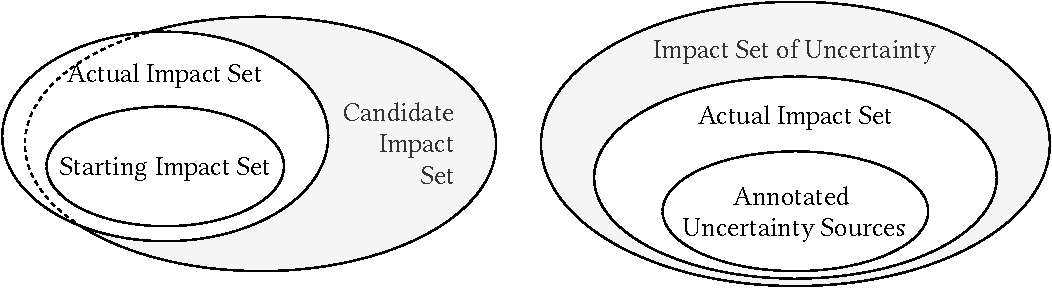
\includegraphics[width=\linewidth]{figures/chapter6/impactset.pdf}
    \caption{Informally illustrated relation of the different sets of change impact analysis (left) and uncertainty impact analysis (right).}
    \label{fig:impactanalysis:representing:sets}
\end{figure}

The \ac{AIS} represents the elements, that are actually impacted by the uncertainty sources in the \ac{SIS} and can violate confidentiality.
This set includes all elements from the \ac{SIS}, but can additionally contain elements that are directly or indirectly affected.
However, we can only estimate this set.
Similarly to change impact analysis, an uncertainty impact analysis yields a \ac{CIS}, which represents an estimation of potentially impacted elements.
Here, we require a more strict relation. 
While change impact analysis may underestimate the \ac{CIS} compared to the \ac{AIS}, uncertainty impact analysis regarding confidentiality shall always overestimate the \ac{CIS}.
Put simply, an ignored impact of uncertainty could lead to overlooked confidentiality violations.
Especially regarding security-related quality properties like confidentiality, high recall can be more important than high precision \cite{hahner_architecture-based_2023}.
Additionally, the uncertainty impact analysis is used for an \emph{early} prediction and assessment of uncertainty, not for precise analysis, see \autoref{sec:overview:procedure}.
This has to be considered in defining the propagation rules for uncertainty.
For the sake of simplicity, we refer to the \ac{AIS} as the actual impact set and to the \ac{CIS} simply as \emph{impact set} of uncertainty.
The relation of the terminology of both analyses is illustrated in \autoref{fig:impactanalysis:representing:sets}.

In the following, we describe propagation rules for all annotation targets of uncertainty sources in the \ac{PCM}.
They have to be described separately for each relevant \ac{PCM} element as they are specific to the \ac{ADL} \ac{PCM}.
Nevertheless, the general concept of architectural uncertainty propagation is generalizable \cite{camara_uncertainty_2024}.
The goal of uncertainty propagation in the architectural model is to identify all uncertainty-afflicted elements of the software architecture, which are later represented by the extracted \ac{DFD} \cite{seifermann_architectural_2022}.
In most cases, this means starting with propagation rules from change impact analysis and then identifying relevant \ac{SEFF} actions, as these are relevant to the \ac{DFD} extraction of \textcite{seifermann_architectural_2022}.
This step is important because of the abstraction gap between the representations of \acp{DFD} and the \ac{PCM}, see \autoref{sec:impactanalysis:representing}.
By identifying those elements, the coupling of the architectural impact analysis with the propagation of uncertainty in \acp{DFD} is simplified.
Only propagating uncertainty in \acp{DFD} is not sufficient due to the missing information compared to architectural models.

\finding{Uncertainty impact analysis regarding confidentiality in architectural models consists of two steps.
First, identifying directly and indirectly affected elements, following the propagation rules of change impact analysis.
Second, identifying originating elements of the transformation to \acp{DFD}, which are relevant for further propagation.}


\subsection{Uncertainty Propagation of Component Uncertainty}

\emph{Component} uncertainty can only be annotated to \emph{AssemblyContexts}, which simplifies the propagation logic.
\autoref{alg:impactanalysis:component} shows the propagation algorithm.
Every propagation algorithm is called with the annotated uncertainty source contained in the parameter \emph{uncertainty} and the \ac{PCM} model contained in the parameter \emph{model}.
We always start by creating an empty list of results and retrieving the model element that has been annotated with the uncertainty source, following the relation specified in \autoref{fig:impactanalysis:representing:relation}.

\begin{algorithm}
    \caption{Algorithm for component uncertainty propagation}
    \label{alg:impactanalysis:component}
    \begin{algorithmic}[1]
        \Procedure{\function{propagateComponentUncertainty}}{$\var{uncertainty}, \var{model}$}
            \algindentskip
            \State $\var{result} \gets \emptyset$
            \State $\var{assemblyContext} \gets \function{getAnnotatedElement}(\var{uncertainty}, \var{model})$
            \State $\var{component} \gets \function{getRepositoryComponent}(\var{assemblyContext}, \var{model})$ \label{alg:impactanalysis:component:4}
            \State $\var{seffs} \gets \function{getSEFFs}(\var{component}, \var{model})$ \label{alg:impactanalysis:component:5}
            \algblockskip

            \For{$\var{seff} \in \var{seffs}$} \label{alg:impactanalysis:component:6} \Comment{Component uncertainty affects all SEFFs of a component}
                \State $\var{startAction} \gets \function{retrieveStartAction}(\var{seff}, \var{model})$
                \State $\var{result} \gets \var{result} \cup \setted{\var{startAction}}$ \label{alg:impactanalysis:component:11}
            \EndFor
            \algblockskip
        
            \State \Return{$\function{applyToAssembly}(\var{result},\var{assemblyContext})$} \label{alg:impactanalysis:component:10}
            \algindentskip
        \EndProcedure   
    \end{algorithmic}
\end{algorithm}

In the case of \emph{AssemblyContexts}, which represent instantiated components, we retrieve the component type from the \ac{PCM} component repository model in \autoref{alg:impactanalysis:component:4} and then query for its \acp{SEFF} in \autoref{alg:impactanalysis:component:5}.
A component provides one \ac{SEFF} for each signature of a provided interface.
For instance, in our running example, the \emph{Database Service} provides \acp{SEFF} for the operations \emph{queryInventory} and \emph{storePurchaseData}, see \autoref{fig:impactanalysis:representing:example}.

\begin{algorithm}
    \caption{Algorithm for retrieving the initial StartAction of a \ac*{SEFF}}
    \label{alg:impactanalysis:helperseff}
    \begin{algorithmic}[1]
        \Procedure{\function{retrieveStartAction}}{$\var{seff}, \var{model}$}
            \algindentskip
            \State $\var{actions} \gets \function{getActions}(\var{seff}, \var{model})$
            \For{$\var{action} \in \var{actions}$}
                \If{$\function{typeOf}(\var{action}) = \datatype{StartAction}$} \label{alg:impactanalysis:helperseff:4}
                    \State $\var{startAction} \gets \var{action}$ \Comment{The first start action is the start of the SEFF}
                    \State \Return{$\var{startAction}$}
                \EndIf
            \EndFor
            \algindentskip
        \EndProcedure   
    \end{algorithmic}
\end{algorithm}

From the perspective of the change impact analysis, these \acp{SEFF} are impacted by a change to the component.
To close the gap to the representation in \acp{DFD}, we need to retrieve the initial actions of all \acp{SEFF} that are represented as \ac{DFD} nodes \cite{seifermann_architectural_2022}.
We show this separately in \autoref{alg:impactanalysis:helperseff} because we reuse this functionality several times in other algorithms.
A \ac{SEFF} contains actions that represent its behavior, comparable to \ac{UML} activity diagrams.
The initial actions have the \ac{PCM} element type \emph{StartAction}, see \autoref{alg:impactanalysis:helperseff:4}.
Using the functionality described in \autoref{alg:impactanalysis:helperseff}, we iterate over all \acp{SEFF}, starting in \autoref{alg:impactanalysis:component:6}.
Once we found this action, we add it to the results list in \autoref{alg:impactanalysis:component:11}.
The algorithm ends after all initial \emph{StartActions} of all \acp{SEFF} have been identified and returns the result.

Note that we skip some Palladio \cite{reussner_palladio_2024} implementation details.
First, we do not show required type casts, e.g., from \emph{RepositoryComponent} to \emph{BasicComponent} to retrieve the \acp{SEFF}.
Second, we hide method calls, e.g., to retrieve all actions, a detour from the \ac{SEFF} through its behavior is required.
Third, we skip the handling of the system context.
This step is required because \acp{SEFF} are defined in the \ac{PCM} component repository model and could be instantiated in multiple assemblies.
However, we are only interested in those actions representing the \emph{AssemblyContext} that is annotated with the component uncertainty.
We illustrate this with a method call of \emph{applyToAssembly} in \autoref{alg:impactanalysis:component:10}.
Last, we assume well-formed \ac{PCM} models without errors.
All of these details would only greatly increase the size of the algorithms without contributing to their understandability.
To see the detailed implementation of all algorithms, please look into the data set \cite{dataset}.


\subsection{Uncertainty Propagation of Interface Uncertainty}

\emph{Interface} uncertainty can be annotated to full interfaces or selected signatures.
Uncertainty affecting interfaces results in a wide impact due to their central role in software systems.
The propagation of interface uncertainty requires the most extensive algorithm.
We split the propagation into three parts.
First, we identify all components and their actions that implement the interface in \autoref{alg:impactanalysis:interface:startaction}.
Second, we identify all actions that represent calls to the interface in \autoref{alg:impactanalysis:interface:externalcallaction}.
Third, we identify all system calls from \emph{UsageScenarios} to the interface in \autoref{alg:impactanalysis:interface:entrylevelsystemcall}.
These three steps are required as we cannot make any assumptions on the usage of the interface, e.g., to wire components or to represent a user interface.
By combining these three steps, we specify the algorithm for interface uncertainty propagation in \autoref{alg:impactanalysis:interface}.

\emph{Interface} uncertainty affects the \ac{PCM} component repository model and is not limited single assemblies like \emph{Component} uncertainty.
Thus, the impact set can be even bigger, as all \emph{AssemblyContexts} of a component can be affected.
Put simply, if a component that is used multiple times in a software system has uncertainty in its interface, it affects all instances of this component and also all components that depend on these instances.

\begin{algorithm}
    \caption{Algorithm for retrieving all StartActions that describe a signature}
    \label{alg:impactanalysis:interface:startaction}
    \begin{algorithmic}[1]
        \Procedure{\function{retrieveStartActionsBySignature}}{$\var{signature}, \var{model}$}
            \algindentskip
            \State $\var{result} \gets \emptyset$
            \State $\var{allComponents} \gets \function{getAllRepositoryComponents}(\var{model})$
            \algblockskip

            \For{$\var{component} \in allComponents$}
                \State $\var{seffs} \gets \function{getSEFFs}(\var{component}, \var{model})$
                \For{$\var{seff} \in \var{seffs}$} \Comment{Find called StartActions}
                    \If{$\function{getDescribedSignature}(\var{seff}, \var{model}) = signature$} \label{alg:impactanalysis:interface:startaction:7}
                        \State $\var{startAction} \gets \function{retrieveStartAction}(\var{seff}, \var{model})$ \label{alg:impactanalysis:interface:startaction:8}
                        \State $\var{result} \gets \var{result} \cup \setted{\var{startAction}}$
                    \EndIf
                \EndFor
            \EndFor
            \algblockskip

            \State \Return{$\var{result}$}
            \algindentskip
        \EndProcedure   
    \end{algorithmic}
\end{algorithm}

\autoref{alg:impactanalysis:interface:startaction} shows the algorithm to identify all \acp{SEFF} that implement a signature of an interface.
Regarding change impact analysis, this resembles the adaption of all implementations of an interface, e.g., due to a rename of a signature.
We iterate over all \acp{SEFF} of all components in the \ac{PCM} component repository model to find matching \emph{StartActions}.
The retrieval logic is similar to \emph{Component} uncertainty with two important distinctions.
First, the retrieval is not limited to a single \emph{AssemblyContext} but includes all components.
Second, the algorithm only considers \acp{SEFF} that implement the given signature of the interface.
Not necessarily all \acp{SEFF} of a component have to implement an interface because components can also provide multiple interfaces.
This filter is realized in \autoref{alg:impactanalysis:interface:startaction:7}.
Afterward, we retrieve the \emph{StartAction} in \autoref{alg:impactanalysis:interface:startaction:8} using the logic described with \autoref{alg:impactanalysis:helperseff}.
In our running example, retrieving the \emph{StartAction} of the \ac{SEFF} that implements the signature \emph{queryInventory} would yield a \emph{StartAction} of the component \emph{Database Service} because this component provides the interface that contains the signature, see \autoref{fig:impactanalysis:representing:example}.

\begin{algorithm}
    \caption{Algorithm for retrieving all ExternalCallActions that call a signature}
    \label{alg:impactanalysis:interface:externalcallaction}
    \begin{algorithmic}[1]
        \Procedure{\function{retrieveExternalCallsToSignature}}{$\var{signature}, \var{model}$}
            \algindentskip
            \State $\var{result} \gets \emptyset$
            \State $\var{allComponents} \gets \function{getAllRepositoryComponents}(\var{model})$
            \algblockskip

            \For{$\var{component} \in allComponents$} \Comment{Iterate over all available actions} \label{alg:impactanalysis:interface:externalcallaction:4}
                \State $\var{seffs} \gets \function{getSEFFs}(\var{component}, \var{model})$
                \For{$\var{seff} \in \var{seffs}$} 
                    \State $\var{actions} \gets \function{getActions}(\var{seff}, \var{model})$
                    \For{$\var{action} \in \var{actions}$} \Comment{Find calling ExternalCallActions}
                        \If{$\function{typeOf}(\var{action}) = \datatype{ExternalCallAction}$} 
                            \If{$\function{getCalledSignature}(\var{action}, \var{model}) = signature$} \label{alg:impactanalysis:interface:externalcallaction:10}
                                \State $\var{result} \gets \var{result} \cup \setted{\var{action}}$
                            \EndIf
                        \EndIf
                    \EndFor
                \EndFor
            \EndFor
            \algblockskip

            \State \Return{$\var{result}$}
            \algindentskip
        \EndProcedure   
    \end{algorithmic}
\end{algorithm}

\autoref{alg:impactanalysis:interface:externalcallaction} shows the algorithm to identify all system actions that call a signature of an interface.
In the \ac{PCM}, calls between components are modeled in \ac{SEFF} using \emph{ExternalCallActions} \cite{becker_palladio_2009}.
Regarding change impact analysis, this resembles adapting the call to an interface after the interface has changed.
To identify the impacted \emph{ExternalCallActions}, we have to iterate over all available actions starting in \autoref{alg:impactanalysis:interface:externalcallaction:4}.
This is achieved by iterating over all components, all of its \acp{SEFF} and over all of their actions.
If the action represents an \emph{ExternalCallAction}, we check its called signature in \autoref{alg:impactanalysis:interface:externalcallaction:10}.
All actions that fit these conditions are added to the result.
These would also be part of the \ac{CIS} of the change impact analysis \ac{KAMP} \cite{busch_architecture-based_2020}.
In our running example detailed in \autoref{fig:impactanalysis:representing:example}, an \emph{ExternalCallAction} is used after the processing of the purchase in the \emph{Online Shop} to initiate the storing of the data in the \emph{Database Service}.
To minimize costly iterations, concrete implementations of this algorithm can cache identified \emph{ExternalCallActions} or use other query methods, which return all occurrences of an element type within a model \cite{dataset}---we show the generic approach of iterating over all components to keep the algorithm as simple as possible.


\begin{algorithm}
    \caption{Algorithm for retrieving all EntryLevelSystemCalls that call a signature}
    \label{alg:impactanalysis:interface:entrylevelsystemcall}
    \begin{algorithmic}[1]
        \Procedure{\function{retrieveEntryCallsToSignature}}{$\var{signature}, \var{model}$}
        \algindentskip
        \State $\var{result} \gets \emptyset$
        \State $\var{allUsageScenarios} \gets \function{getAllUsageScenarios}(\var{model})$
        \algblockskip

        \For{$\var{usageScenario} \in allUsageScenarios$} \label{alg:impactanalysis:interface:entrylevelsystemcall:4}
            \State $\var{actions} \gets \function{getActions}(\var{usageScenario}, \var{model})$
            \For{$\var{action} \in \var{actions}$} \Comment{Find calling EntryLevelSystemCalls}
                \If{$\function{typeOf}(\var{action}) = \datatype{EntryLevelSystemCall}$} \label{alg:impactanalysis:interface:entrylevelsystemcall:7}
                    \If{$\function{getCalledSignature}(\var{action}, \var{model}) = signature$} \label{alg:impactanalysis:interface:entrylevelsystemcall:8}
                        \State $\var{result} \gets \var{result} \cup \setted{\var{action}}$
                    \EndIf
                \EndIf
            \EndFor
        \EndFor
        \algblockskip

        \State \Return{$\var{result}$}
        \algindentskip
        \EndProcedure   
    \end{algorithmic}
\end{algorithm}

\autoref{alg:impactanalysis:interface:entrylevelsystemcall} shows the algorithm to identify all calls from a \emph{UsageScenario} to a signature of an interface.
In the \ac{PCM}, calls to the the system are modeled using \emph{EntryLevelSystemCalls}.
As discussed above, this step is required as we cannot assume that an interface is only used between components.
This step is also performed by change impact analysis \cite{busch_architecture-based_2020}.
To identify relevant \emph{EntryLevelSystemCalls}, we iterate over all actions of all \emph{UsageScenarios}, starting in \autoref{alg:impactanalysis:interface:entrylevelsystemcall:4}.
We first check for the type of the action in \autoref{alg:impactanalysis:interface:entrylevelsystemcall:7}, and if it represents an \emph{EntryLevelSystemCall}, we check the called signature in \autoref{alg:impactanalysis:interface:entrylevelsystemcall:8}.
Afterward, the actions are added to the result.
This procedure closely resembles the retrieval of impacted \emph{ExternalCallActions}.
Here, the main difference is that we do not analyze the behavior of a component but the user behavior that is modeled in the \ac{PCM} usage model.
In our running example, all calls of the \emph{Customer} to the \emph{Online Shop} are modeled using \emph{EntryLevelSystemCalls}, e.g., the querying of items.


\begin{algorithm}
    \caption{Algorithm for interface uncertainty propagation}
    \label{alg:impactanalysis:interface}
    \begin{algorithmic}[1]
        \Procedure{\function{propagateInterfaceUncertainty}}{$\var{uncertainty}, \var{model}$}
        \algindentskip
        \State $\var{result} \gets \emptyset$
        \State $\var{affectedSignatures} \gets \emptyset$
        \State $\var{annotatedElement} \gets \function{getAnnotatedElement}(\var{uncertainty}, \var{model})$ \label{alg:impactanalysis:interface:4}
        \algblockskip

        \Switch{$\function{typeOf}(\var{annotatedElement})$} \label{alg:impactanalysis:interface:5}
            \Case{$\datatype{Signature}$}
                \State $\var{affectedSignatures} \gets \setted{\var{annotatedElement}}$
            \EndCase
            \Case{$\datatype{Interface}$} \Comment{Decompose the interface}
                \State $\var{affectedSignatures} \gets \function{getSignatures}(\var{annotatedElement}, \var{model})$
            \EndCase
        \EndSwitch
        \algblockskip

        \For{$\var{signature} \in \var{affectedSignatures}$} \Comment{Combine the three retrieval steps} \label{alg:impactanalysis:interface:10}
            \State $\var{result} \gets \var{result} \cup \function{retrieveStartActionsBySignature}(\var{signature}, \var{model})$
            \State $\var{result} \gets \var{result} \cup \function{retrieveExternalCallsToSignature}(\var{signature}, \var{model})$
            \State $\var{result} \gets \var{result} \cup \function{retrieveEntryCallsToSignature}(\var{signature}, \var{model})$
        \EndFor
        \algblockskip

        \State \Return{$\var{result}$}
        \algindentskip
        \EndProcedure   
    \end{algorithmic}
\end{algorithm}

We combine the algorithms \ref{alg:impactanalysis:interface:startaction}, \ref{alg:impactanalysis:interface:externalcallaction}, and \ref{alg:impactanalysis:interface:entrylevelsystemcall} to specify the propagation algorithm for \emph{Interface} uncertainty in \autoref{alg:impactanalysis:interface}.
After retrieving the element that has been annotated with uncertainty in \autoref{alg:impactanalysis:interface:4}, we perform a type check in \autoref{alg:impactanalysis:interface:5}.
If the annotated element is an \emph{Interface}, we decompose the interface into its signatures and add it to the list of affected signatures.
If the annotated element is a \emph{Signature}, this list only consists of this single signature.
This resembles one propagation step from change impact analysis \cite{rostami_architecture-based_2017,busch_architecture-based_2020} and enables the treatment of both annotations targets similarly in the following.
Put simply, annotating a signature instead of an interface increases the precision of the result but only has a negligible effect on the propagation logic.
Afterward, we iterate over all signatures in \autoref{alg:impactanalysis:interface:10}.
For each signature, we perform the three retrieval tasks, i.e., retrieving affected \emph{StartActions}, \emph{ExternalCallActions}, and \emph{EntryLevelSystemCalls}.
The combined result is returned from the algorithm.
Note that this does not cause any typing problems, as we expect \emph{any} action as a result, similarly to all other propagation algorithms.

In our running example, an \emph{Interface} uncertainty that has been annotated to the interface between the \emph{Online Shop} and the \emph{Database Service} components would yield affected elements from both components.
This includes \emph{StartActions} from \acp{SEFF} of all implementations of operations specified in the interface and also \emph{ExternalCallActions} to these operations.
However, as this interface is only used between components, no \emph{EntryLevelSystemCalls} would be directly affected.
Note that there is no call to \emph{applyToAssembly} as we do not limit the impact of uncertainty to a single assembly.
For instance, if the \emph{Database Service} component would be used in multiple locations in the system, all instances would be affected by the uncertainty.

Similarly to the propagation of \emph{Component} uncertainty shown in \autoref{alg:impactanalysis:component}, we hide implementation details.
This includes chained method calls, e.g., to retrieve all actions of a \emph{UsageScenario}, a detour over its behavior is required \cite{reussner_palladio_2024}.
Although all algorithms presented in this section contain several loops, we do not expect problems regarding their scalability in practice.
First, the sets to iterate over are usually small, e.g., because a properly defined interface only contains a small number of signatures \cite{martin_clean_2017}.
Second, there are many ways to speed up the implementation, e.g., by using caches, or by integrating the extracted \acp{DFD} early in the propagation to filter potential candidates.
We apply many of these optimizations in our implementation that are available in the data set \cite{dataset}.


\subsection{Uncertainty Propagation of Connector Uncertainty}

\begin{algorithm}
    \caption{Algorithm for connector uncertainty propagation}
    \label{alg:impactanalysis:connector}
    \begin{algorithmic}[1]
        \Procedure{\function{propagateConnectorUncertainty}}{$\var{uncertainty}, \var{model}$}
            \algindentskip
            \State $\var{result} \gets \emptyset$
            \State $\var{connector} \gets \function{getAnnotatedElement}(\var{uncertainty}, \var{model})$
            \State $\var{interface} \gets \function{getInterface}(\var{connector}, \var{model})$ \label{alg:impactanalysis:connector:4}
            \State $\var{signatures} \gets \function{getSignatures}(\var{interface}, \var{model})$
            \State $\var{calledAssembly} \gets \function{getProvidingAssemblyContext}(\var{connector}, \var{model})$ \label{alg:impactanalysis:connector:6}
            \algblockskip

            \For{$\var{signature} \in \var{signatures}$}  \Comment{Find called StartActions} \label{alg:impactanalysis:connector:7}
                \State $\var{actions} \gets \function{retrieveStartActionsBySignature}(\var{signature}, \var{model})$
                \State $\var{result} \gets \var{result} \cup \function{applyToAssembly}(\var{actions},\var{calledAssembly})$ \label{alg:impactanalysis:connector:9}
            \EndFor
            \algblockskip

            \Switch{$\function{typeOf}(\var{connector})$} \label{alg:impactanalysis:connector:11}
                \Case{$\datatype{AssemblyConnector}$}
                    \State $\var{callingAssembly} \gets \function{getRequiringAssemblyContext}(\var{connector}, \var{model})$ \label{alg:impactanalysis:connector:13}
                    \algblockskip
                    \For{$\var{signature} \in \var{signatures}$}  \Comment{Find calling ExternalCallActions} \label{alg:impactanalysis:connector:14}
                        \State $\var{actions} \gets \function{retrieveExternalCallsToSignature}(\var{signature}, \var{model})$
                        \State $\var{result} \gets \var{result} \cup \function{applyToAssembly}(\var{actions},\var{callingAssembly})$ \label{alg:impactanalysis:connector:16}
                    \EndFor
                    \algblockskip
                \EndCase
                \Case{$\datatype{ProvidedDelegationConnector}$} 
                    \State $\var{delegatedContext} \gets \function{getDelegatedContext}(\var{connector}, \var{model})$ \label{alg:impactanalysis:connector:19}
                    \algblockskip
                    \For{$\var{signature} \in \var{signatures}$}  \Comment{Find calling EntryLevelSystemCalls} \label{alg:impactanalysis:connector:20}
                        \State $\var{actions} \gets \function{retrieveEntryCallsToSignature}(\var{signature}, \var{model})$
                        \State $\var{result} \gets \var{result} \cup \function{applyToAssembly}(\var{actions},\var{delegatedContext})$ \label{alg:impactanalysis:connector:22}
                    \EndFor
                    \algblockskip
                \EndCase
            \EndSwitch
            \algblockskip

            \State \Return{$\var{result}$}
            \algindentskip
        \EndProcedure   
    \end{algorithmic}
\end{algorithm}

\emph{Connector} uncertainty can be annotated to \emph{AssemblyConnectors} and \emph{ProvidedDelegationConnectors}.
\autoref{alg:impactanalysis:connector} shows the propagation algorithm.
Uncertainty affecting connectors behaves comparable to \emph{Interface} uncertainty.
It impacts both the called component and the calling entity, which can be another component or a user.
The main difference is that connectors are specific to assemblies and modeled in the \ac{PCM} system model.
We can reuse the logic defined for \emph{Interface} uncertainty hereabove but we have to relate the results to the correct \emph{AssemblyContexts}.

A \emph{Connector} represents the wiring of two entities within a software system, expressed, e.g., using the ball and socket notation of \ac{UML} component diagrams as shown in \autoref{fig:runningexample:architecture}.
All connectors are based on an interface that we retrieve in \autoref{alg:impactanalysis:connector:4}.
In the \ac{PCM}, we support \emph{AssemblyConnectors} between two components and \emph{ProvidedDelegationConnectors} that can be referred to outside the system in \emph{UsageScenarios}.

Independent of its type, a connector always has a providing \emph{AssemblyContext}, representing the component that implements the provided interface.
This called \emph{AssemblyContext} is retrieved in \autoref{alg:impactanalysis:connector:6}.
Afterward, we find all called \emph{StartActions} beginning in \autoref{alg:impactanalysis:connector:7}.
Here, we can reuse the logic defined for \emph{Interface} uncertainty in \autoref{alg:impactanalysis:interface:startaction}.
The only difference is that we are only interested in those \emph{StartActions} that represent the connected \emph{AssemblyContext}.
This is realized in \autoref{alg:impactanalysis:connector:9}, similarly to \emph{Component} uncertainty.

Afterward, we address the calling side, starting in \autoref{alg:impactanalysis:connector:11}.
In the case of an \emph{AssemblyConnector}, we retrieve the calling assembly that requires the interface represented by the connector in \autoref{alg:impactanalysis:connector:13}.
We use the logic defined for \emph{Interface} uncertainty in \autoref{alg:impactanalysis:interface:externalcallaction} to find the according \emph{ExternalCallActions} in \autoref{alg:impactanalysis:connector:14}.
Again, we have to apply the correct \emph{AssemblyContext}.
This time, this is achieved using the calling assembly in \autoref{alg:impactanalysis:connector:16}.
In the case of a \emph{ProvidedDelegationConnector}, we proceed with the retrieval of \emph{EntryLevelSystemCalls}.
Here, we are only interested in the provided delegation of the system interface, which is retrieved in \autoref{alg:impactanalysis:connector:19}.
After receiving candidate \emph{ExternalCallActions} in \autoref{alg:impactanalysis:connector:20}, we apply again the correct context in \autoref{alg:impactanalysis:connector:22}.

Put simply, to propagate \emph{Connector} uncertainty we proceed as if the interface that is represented would be affected by \emph{Interface} uncertainty.
Every potentially impacted action is then applied to the correct \emph{AssemblyContext}, either called or calling.
Regarding change impact analysis, this resembles the required changes both in the component that implements an interface and the component requiring an interface.
Besides the handling of \emph{AssemblyContexts} and indirection from the \emph{Connector} to interfaces, another difference is the distinction of the connector type.
When propagating \emph{Interface} uncertainty, we only use the \ac{PCM} component repository model and we cannot make assumptions on the interface use, i.e., whether the interface is only used between components or also in \emph{UsageScenarios}.
Opposite to this, \emph{Connectors} are part of the \ac{PCM} system model that models this information.
Thus, we are not required to handle all cases and can either retrieve \emph{ExternalCallActions} or \emph{EntryLevelSystemCalls}, but not both.
In our running example, the results of an \emph{Interface} uncertainty and a \emph{Connector} uncertainty annotated between the \emph{Online Shop} and \emph{Database Service} components are identical because both components are only referred by a single \emph{AssemblyContext}.
Similarly to the other algorithms, we simplified some chained method calls and we refer to the data set for more details \cite{dataset}.


\subsection{Uncertainty Propagation of External Uncertainty}

\begin{algorithm}
    \caption{Algorithm for external uncertainty propagation}
    \label{alg:impactanalysis:external}
    \begin{algorithmic}[1]
        \Procedure{\function{propagateExternalUncertainty}}{$\var{uncertainty}, \var{model}$}
        \algindentskip
        \State $\var{result} \gets \emptyset$
        \State $\var{annotatedElement} \gets \function{getAnnotatedElement}(\var{uncertainty}, \var{model})$
        \algblockskip

        \Switch{$\function{typeOf}(\var{annotatedElement})$} \label{alg:impactanalysis:external:4}
            \Case{$\datatype{UsageScenario}$}
                \State $\var{actions} \gets \function{getActions}(\var{annotatedElement}, \var{model})$ \label{alg:impactanalysis:external:6}
                \For{$\var{action} \in \var{actions}$} \Comment{Find all EntryLevelSystemCalls}
                    \If{$\function{typeOf}(\var{action}) = \datatype{EntryLevelSystemCall}$}
                        \State $\var{result} \gets \var{result} \cup \setted{\var{action}}$
                    \EndIf
                \EndFor
                \algblockskip
            \EndCase
            \Case{$\datatype{ResourceContainer}$} 
                \State $\var{allAssemblyContexts} \gets \function{getAllAssemblyContexts}(\var{model})$ \label{alg:impactanalysis:external:13}
                \For{$\var{context} \in \var{allAssemblyContexts}$} \Comment{Find all actions}
                    \If{$\function{getAllocation}(\var{context}, \var{model}) = annotatedElement$} \label{alg:impactanalysis:external:15}
                        \State $\var{component} \gets \function{getRepositoryComponent}(\var{context}, \var{model})$
                        \State $\var{seffs} \gets \function{getSEFFs}(\var{component}, \var{model})$
                        \For{$\var{seff} \in \var{seffs}$}
                            \State $\var{actions} \gets \function{getActions}(\var{seff}, \var{model})$ 
                            \State $\var{result} \gets \var{result} \cup \function{applyToAssembly}(\var{actions},\var{context})$ \label{alg:impactanalysis:external:20}
                        \EndFor
                    \EndIf
                \EndFor
            \EndCase
        \EndSwitch
        \algblockskip
        \State \Return{$\var{result}$}
        \algindentskip
        \EndProcedure   
    \end{algorithmic}
\end{algorithm}

\emph{External} uncertainty can be annotated to \emph{ResourceContainers} and \emph{UsageScenarios}.
\autoref{alg:impactanalysis:external} shows the propagation algorithm.
\emph{ResourceContainers} are part of the \ac{PCM} resource environment model and \emph{UsageScenarios} are part of the \ac{PCM} usage model.
Although the propagation logic differs, it states the same: Find all actions that belong to the element that has been annotated with \emph{external} uncertainty.
Put simply, if a resource container or a user is affected by uncertainty, we cannot trust any of their actions.

The algorithm starts with a large switch statement in \autoref{alg:impactanalysis:external:4}.
In the case of an annotated \emph{UsageScenario}, we iterate over all of its actions, starting in \autoref{alg:impactanalysis:external:6}.
This is similar to the identification of relevant \emph{EntryLevelSystemCalls} of \emph{Interface} or \emph{Connector} uncertainty.
The major difference is that we do not filter for a specific signature, but add all identified \emph{EntryLevelSystemCalls}, as they could all be affected by uncertainty.
We only consider \emph{EntryLevelSystemCalls} as they represent the only user actions that are considered in the extraction of \acp{DFD} \cite{seifermann_architectural_2022}.

In the case of an annotated \emph{ResourceContainer}, we have to identify all \emph{AssemblyContexts} that are allocated on this container.
We retrieve all \emph{AssemblyContexts} from the \ac{PCM} system model in \autoref{alg:impactanalysis:external:13} and iterate over them.
For each assembly, we check its allocation using the \ac{PCM} allocation model in \autoref{alg:impactanalysis:external:15}.
If an \emph{AssemblyContext} is deployed on the \emph{ResourceContainer} that has been annotated with the uncertainty, we add all of its actions to the result list in \autoref{alg:impactanalysis:external:20}.
This step is comparable to the propagation of \emph{Component} uncertainty.
However, we do not limit the propagation to \emph{StartActions} as every action could be affected by uncertainty.

In the running example, an \emph{external} uncertainty annotated to the \emph{ResourceContainer} where the \emph{Online Shop} gets deployed would affect all of its actions.
In the simplified illustration shown in \autoref{fig:impactanalysis:representing:example}, this would include \emph{process request}, \emph{display items}, and \emph{process purchase}.
\emph{External} uncertainty can have a particularly large impact if many \emph{AssemblyContexts} are deployed on a single \emph{ResourceContainers} affected by uncertainty.
The same applies to \emph{UsageScenarios} with many \emph{EntryLevelSystemCalls}.
Again, we simplified some methods shown in the algorithm to increase understandability.
Interestingly, \emph{external} uncertainty requires the connection of all \ac{PCM} models, namely the usage model, system model, component repository model including \acp{SEFF}, the resource environment model, and the allocation model.
However, this is not surprising, as \emph{external} uncertainty affects the system context in different places and is propagated into the software system.


\subsection{Uncertainty Propagation of Behavior Uncertainty}

\begin{algorithm}
    \caption{Algorithm for behavior uncertainty propagation}
    \label{alg:impactanalysis:behavior}
    \begin{algorithmic}[1]
        \Procedure{\function{propagateBehaviorUncertainty}}{$\var{uncertainty}, \var{model}$}
        \algindentskip
        \State $\var{result} \gets \emptyset$
        \State $\var{annotatedElement} \gets \function{getAnnotatedElement}(\var{uncertainty}, \var{model})$
        \algblockskip

        \Switch{$\function{typeOf}(\var{annotatedElement})$} \label{alg:impactanalysis:behavior:4}
            \Case{$\datatype{EntryLevelSystemCall}$}
                \State $\var{result} \gets \var{result} \cup \setted{\var{annotatedElement}}$
            \EndCase
            \Case{$\datatype{ExternalCallAction}$} 
                \State $\var{result} \gets \var{result} \cup \setted{\var{annotatedElement}}$
            \EndCase
            \Case{$\datatype{SetVariableAction}$} 
                \State $\var{result} \gets \var{result} \cup \setted{\var{annotatedElement}}$
            \EndCase
            \Case{$\datatype{BranchAction}$} \label{alg:impactanalysis:behavior:11}
                \State $\var{actions} \gets \function{getActions}(\var{annotatedElement}, \var{model})$
                \For{$\var{action} \in \var{actions}$}
                    \If{$\function{typeOf}(\var{action}) = \datatype{StartAction}$}
                        \State $\var{result} \gets \var{result} \cup \setted{\var{action}}$
                    \EndIf
                \EndFor
            \EndCase
        \EndSwitch
        \algblockskip

        \State \Return{$\var{result}$}
        \algindentskip
        \EndProcedure   
    \end{algorithmic}
\end{algorithm}

\emph{Behavior} uncertainty can be annotated to \emph{EntryLevelSystemCall}, \emph{ExternalCallActions}, \emph{SetVariableAction}, and \emph{BranchActions}.
\autoref{alg:impactanalysis:behavior} shows the propagation algorithm.
Despite being the uncertainty source with the most possible annotation targets, the propagation algorithm is simple.
The algorithm is realized using one big switch statement starting in \autoref{alg:impactanalysis:behavior:4}.
In the case of \emph{EntryLevelSystemCalls}, \emph{ExternalCallActions} and \emph{SetVariableActions}, no propagation is required and the annotated elements can directly be added to the result.
The reason for this simplicity is that all three elements are directly represented in the extracted \ac{DFD} \cite{seifermann_architectural_2022}.
Thus, no further architectural propagation is required as the transitive impact can be calculated purely in the \ac{DFD}-based uncertainty propagation.
In the running example, a \emph{behavior} uncertainty annotated to the \emph{ExternalCallAction} to trigger the storing of data thus only contains the action itself as a result of the architectural propagation.

Only uncertainty annotated to \emph{BranchActions} requires additional architectural propagation, starting in \autoref{alg:impactanalysis:behavior:11}.
These actions encapsulate inner sequences of actions, called \emph{BranchTransitions}, that represent the behavior of the \ac{SEFF} if the conditions for one branch are met.
There is no upper limit for the number of \emph{BranchTransitions}.
Thus, we retrieve all actions that are part of all transitions of the \emph{BranchAction} and filter for \emph{StartActions} that are added to the result.
Because all actions are part of the \ac{PCM} component repository model, no handling of \emph{AssemblyContexts} is required.
Note that this does \emph{not} imply that \emph{Behavior} uncertainty generally has a narrower impact on confidentiality.
This only implies that this uncertainty type has a narrower impact using uncertainty propagation in architectural models.
To comprehensively analyze the impact of uncertainty on confidentially, additional \ac{DFD}-based propagation is required, as explained in \autoref{sec:impactanalysis:representing}. 


\subsection{Applying Architectural Uncertainty Impact Analysis}

As explained previously in \autoref{sec:impactanalysis:representing}, we combine uncertainty impact analysis in architectural models and in \ac{DFD} to get comprehensive insights on the impact of uncertainty on confidentiality.
In this section, we introduced all algorithms for architectural propagation of uncertainty.
To conclude, we apply these algorithms on the four annotated uncertainty sources \U{1} -- \U{4} from our running example presented in \autoref{ch:runningexample}.
We introduced the terminology of \ac{SIS}, \ac{AIS}, and \ac{CIS} at the beginning of this section.
The result of the uncertainty impact analysis can be considered as a partial \ac{CIS}, or partial \emph{impact set}, because we still lack the second part of the impact analysis, i.e., the propagation in \acp{DFD}.
Nevertheless, the identified elements of the architectural propagation represent the starting point for the \ac{DFD}-based propagation. 
We present the results of the architectural impact analysis based on the exemplary \ac{SIS} presented in \autoref{table:impactanalysis:sisexample}.

Uncertainty \U{1} affects the user input and is modeled as \emph{Connector} uncertainty.
This uncertainty source is annotated to the \emph{ProvidedDelegationConnector} of the \emph{PurchaseInterface}, which also represents the \ac{SIS}.
We apply the connector uncertainty propagation described in \autoref{alg:impactanalysis:connector}.
The interface that is represented by the \emph{ProvidedDelegationConnector} consists of one signature: \emph{purchaseItem}, to buy items from the online shop.
This operation is implemented in the \emph{Online Shop} component and used in a single \emph{AssemblyContext} of this component.
Thus, there is only one \emph{StartAction} to identify, i.e., the \emph{StartAction} of the \ac{SEFF} that also contains the processing of the purchase prior to its storage in the database.
As \emph{StartActions} are usually not named in \acp{SEFF} \cite{reussner_palladio_2024}, we refer to it as \emph{purchaseItem.start}.
Following the propagation in the calling direction, we identify the \emph{EntryLevelSystemCall} in the \emph{UsageScenario} that represents a customer purchasing items from the shop.
\emph{EntryLevelSystemCalls} are usually named after the interface and signature they call, i.e., \emph{PurchaseInterface.purchaseItem}.
To conclude, our partial impact set after the architectural propagation is $\var{CIS_{U1}} = \setted{\var{purchaseItem.start}, \var{PurchaseInterface.purchaseItem}}$.
Both actions can be directly mapped to the \ac{DFD} \cite{seifermann_architectural_2022} for further propagation.

Uncertainty \U{2} affects the data processing and is modeled as \emph{Behavior} uncertainty.
It is annotated to a \emph{SetVariableAction} of the \ac{SEFF} for processing the purchases of customers in the \emph{Online Shop} component, called \emph{processUserData}.
We apply the behavior uncertainty propagation described in \autoref{alg:impactanalysis:behavior}.
In the case of a \emph{SetVariableAction}, the result of the architectural propagation is the action itself.
Thus, the partial impact set is similar to the \ac{SIS}, i.e., $\var{CIS_{U2}} = \setted{\var{processUserData}}$.
This action can directly be mapped to \acp{DFD}.

Uncertainty \U{3} affects the deployment of the \emph{Database Service} and is modeled as \emph{Component} uncertainty.
It is annotated to the \emph{Database Service} component---to be more precise, to the single \emph{AssemblyContext} that represents this component.
We apply the component uncertainty propagation described in \autoref{alg:impactanalysis:component}.
The architectural propagation of this uncertainty includes identifying all \emph{StartActions} of all provided \acp{SEFF}.
As shown in \autoref{fig:impactanalysis:representing:example}, this component provides one interface with two operations: \emph{queryInventory} to query the information about available items stored in the database, and \emph{storePurchaseData} to store details about purchases in the database.
Similarly to Uncertainty \U{1}, we name the start actions of these two \acp{SEFF} \emph{queryInventory.start} and \emph{storePurchaseData.start}.
Thus, the partial impact set is $\var{CIS_{U3}} = \setted{\var{queryInventory.start}, \var{storePurchaseData.start}}$.

Uncertainty \U{4} represents the provider's trustworthiness of the \emph{CloudService} and is modeled as \emph{External} uncertainty.
It is annotated to the \emph{ResourceContainer} that represents the \emph{CloudService}.
We apply the external uncertainty propagation described in \autoref{alg:impactanalysis:external}.
In this propagation algorithm, we first identify all potentially allocated \emph{AssemblyContexts}.
In the running example, this is the single \emph{AssemblyContext} representing the \emph{Database Service} component.
Afterward, we retrieve all of its actions, as all actions could be potentially affected by the uncertainty.
This includes \emph{StartActions}, \emph{ExternalCallActions}, \emph{SetVariableActions}, and \emph{StopActions}.
This causes the biggest partial impact set, that we briefly show as $\var{CIS_{U4}} = \setted{\var{queryInventory.start}, \var{queryData}, \var{storeData}, \dots, \var{storePurchaseData.stop}}$.
See \autoref{sec:appendix:impactset}, or the data set \cite{dataset} for the comprehensive result.

These partial impact sets show the versatility of the impact of uncertainty on confidentiality.
They also demonstrate the importance of considering the transitive impact of uncertainty.
For instance, Uncertainty \U{2} is propagated only to a single action using the architectural uncertainty impact analysis.
However, invalid data processing can cause other confidentiality violations later in the data flow, e.g., in the database.
Theoretically, this propagation could be realized in architectural models like the \ac{PCM}.
However, the algorithms would be hard to define, complex, and require the handling of many special cases.
Thus, we reuse the mapping from the \ac{PCM} to \acp{DFD} to simplify the further propagation.

Another interesting insight is that some of the impact sets share elements, e.g., \emph{queryInventory.start}.
This is not surprising as these elements represent the data flow and can affect confidentiality.
Regarding the impact analysis, we can freely join single impact sets for further propagation or continue with the result of a single annotated uncertainty.
This decision depends on the software architect's need for a precise or comprehensive impact analysis result.
As we do not alter the modeled software architecture but only annotate uncertainty, we can ignore the \ac{UIP} in this analysis.

\finding{The \acf{UIP} does not affect architectural uncertainty impact analysis.
The propagation results of single uncertainty sources can be merged into joint impact sets.
These sets partially represent the impact on confidentiality and require further propagation along the data flow.}





\section{Uncertainty Impact Analysis for Data Flow Diagrams}%
\label{sec:impactanalysis:dfdpropagation}

In this section, we discuss how uncertainty can be propagated in \acp{DFD} to analyze its impact on confidentiality.
This represents the second half of our architecture-based uncertainty impact analysis \cite{hahner_architecture-based_2023} and can be used together with the propagation of uncertainty in architectural models, presented in the previous section. 
The result of this data flow-based impact analysis is the final \emph{impact set} of uncertainty, an estimation of the actual impact of uncertainty on confidentiality, as discussed in \autoref{sec:impactanalysis:representing}.
In the following, we discuss the propagation by referring to \ac{DFD} nodes.
Although we build on the mapping of \textcite{seifermann_architectural_2022} from \ac{PCM} to \acp{DFD}, the impact analysis could also be applied to \acp{DFD} that are manually defined or that originate from other \acp{ADL}.
This addresses Problem \PR{2}{2}.

The propagation of uncertainty in \ac{DFD} starts at selected nodes, e.g., the results of the uncertainty impact analysis in architectural models or the results of an expert's manual investigation.
Following the terminology introduced in \autoref{sec:impactanalysis:pcmpropagation}, these nodes form a set similar to the \ac{SIS}.
The central propagation rule of uncertainty in \ac{DFD} is simple to define\footnote{This central propagation rule might be simple to define, but it was hard to find. It took several student's theses \cite{benkler_architecture-based_2022,priss_mobility_2022,boltz_architectural_2021,stengel_verfeinerung_2021} and more than one year of research before a consensus was reached.}: Starting at each impacted node, follow the direction of each outgoing flow until a sink is reached.
Add each node on this way to the impact set.
We will present the formal foundations and algorithms for this propagation in the following subsections.
For now, we stay on this informal level to explain the reasoning behind this propagation rule.

\begin{figure}
    \centering
    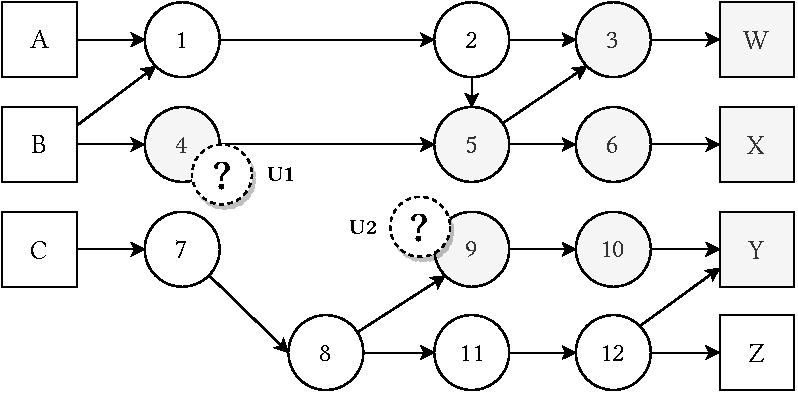
\includegraphics[width=0.8\linewidth]{figures/chapter6/dfd-simple-propagation.pdf}
    \caption{A simple yet versatile \acf*{DFD} with sources (A--C), processes (1--12), sinks (W--Z), and data flows. Uncertainty is denoted by question marks (U1, U2) and the impact set is colored gray.}
    \label{fig:impactanalysis:dfdpropagation:simple}
\end{figure}

\autoref{fig:impactanalysis:dfdpropagation:simple} shows a simplified \ac{DFD} with multiple processes, sources, sinks, and flows, demonstrating the versatility of this notation.
We use this graph instead of the running example because it contains more special cases, e.g., forking and joining data multiple times.
The figure also shows two starting points of the uncertainty propagation, depicted with question marks, named \textbf{U1} and \textbf{U2}.
The annotated nodes represent the starting nodes, i.e., $\var{start_{U1 \cup U2}} = \setted{\var{4,9}}$.
The nodes contained in the impact set are colored gray.
The informally described rule of uncertainty propagation in \acp{DFD} becomes visible here.
Every node that can be reached from the starting nodes is contained in the uncertainty impact set.
In this simplified example, $\var{impact_{U1}} = \setted{3,4,5,6,W,X}$ and $\var{impact_{U2}} = \setted{9,10,Y}$.
Trivially, nodes can also be contained in multiple impact sets if the impact of multiple starting nodes overlaps.
Because the \ac{UIP} does also not affect uncertainty impact analysis in \acp{DFD}, we can merge the impact sets to form the full impact set $\var{impact_{U1 \cup U2}} = \setted{3,4,5,6,9,10,W,X,Y}$.

If we interpret uncertainty as unanticipated change, it can only affect confidentiality at every point that is affected by the change.
Regarding data flows, this requires data to be processed or forwarded by an affected node.
Nodes that have no contact with certain flowing data cannot affect the data's confidentiality, regardless of uncertainty. 
After a data flow has been impacted by uncertainty, we do not make any further assumptions about confidentiality, as any node could or could not violate confidentiality.
In our running example, an uncertain data processing could affect confidentiality directly in the affected processing action, or in a subsequent validation check, or when the data flows to the \emph{Database Service} component, or when the data is stored in the database.
This depends on the modeled software architecture and the specified confidentiality requirements.
However, we can safely exclude any node that cannot be reached by an impacted node following the flow of data.
This includes all previous nodes to the impacted node in the data flow but also all other nodes that cannot be reached.
As software systems usually contain many, independent data flows \cite{seifermann_architectural_2022}, this highly reduces the potential size of the impact set.

\finding{Uncertainty in \acfp{DFD} propagates along data flows, starting from an impacted node until a sink is reached. Preceding nodes and nodes that cannot be reached following the flow of data are not affected.}


\subsection{Formal Foundation for Uncertainty Impact Analysis}

As introduced in \autoref{sec:foundations:dfd} and discussed previously in \autoref{sec:classification:dfd}, \acp{DFD} can be represented using \acp{DAG} \cite{canfora_data_1992}.
Regarding uncertainty impact analysis, we do not require the distinction between primary and secondary uncertainty.
For impact analysis, we only consider \ac{DFD} nodes---or \ac{DAG} vertices---that are either contained or not contained in an impact set.
Thus, we do not alter the \ac{DAG} but only reference a subset of its nodes as an impact set.
We explained these sets at the beginning of this section with \autoref{fig:impactanalysis:dfdpropagation:simple}.

A \ac{DAG} $G = (V, E)$ consist of vertices $V$ and edges $E$.
These represent nodes and data flows, respectively.
Two vertices $u, v \in V$ are strictly partially ordered $v \prec u$ if there exists a path from $v$ to $u$, i.e., a data flow.
This data flow can also be transitive because a strict partial order is irreflexive, asymmetric, and transitive \cite{knuth_art_1997}.
For instance, in \autoref{fig:impactanalysis:dfdpropagation:simple}, $4 \prec 5$ and also $4 \prec 6$ but $4 \nprec B$ and $4 \nprec 9$ because there is no (transitive) data flow.
An induced subgraph $G[V']$ consists of a subset of vertices $V' \subseteq V$ and all edges that have both endpoints in $V'$ \cite{diestel_graph_2017}.
Put simply, in our \acp{DAG}, we start with a vertex and add all vertices that can be reached from this vertex and all the required edges to reach these vertices to the subgraph.
For instance, in \autoref{fig:impactanalysis:dfdpropagation:simple}, $V' = \setted{12, Y, Z}$ induces the subgraph $G' =: G[V']$ with vertices $V'$ and edges $\setted{\flow{12}{Y}, \flow{12}{Z}} = E' \subset E$.

To propagate uncertainty in \acp{DFD}, we start with a vertex $v \in V$ and add it to the impact set $S \subseteq V$.
Then, we iteratively add all vertices that are in the direction of the data flow, i.e., all $u \in V$ where $v \prec u$.
We add all visited edges to the subset $E' \subseteq E$.
The propagation ends once we reached all reachable data sinks, i.e., vertices without outgoing edges.
$S$ then induces a subgraph $G[S]$ with all impacted vertices and all directed edges $E'$ between them.
This subgraph itself forms a \ac{DAG} $G' = (S,E')$.
Note that we do not limit the size of $S$.
In severe cases and wide uncertainty impacts, $S = V$.

In our current example introduced in \autoref{fig:impactanalysis:dfdpropagation:simple}, these induced subgraphs are represented by the nodes that are colored gray.
Uncertainty \textbf{U1} causes the induced subgraph $G_{U1} =: G[S_{U1}]$ with $S_{U1} = \setted{3, 4, 5, 6, W, X}$ and edges $E_{U1} = \setted{\flow{4}{5}, \flow{5}{3}, \flow{5}{6}, \flow{3}{W}, \flow{6}{X}}.$
Uncertainty \textbf{U2} causes the induced subgraph $G_{U2} =: G[S_{U2}]$ with $S_{U2} = \setted{9, 10, Y}$ and edges $E_{U2} = \setted{\flow{9}{10},\flow{10}{Y}}$.
$S_{U1}$ and $S_{U2}$ represent the impact sets presented in the beginning of this section.
They also represent the final impact set of uncertainty regarding confidentiality, i.e, the result of our uncertainty impact analysis.
Note that impact sets can be a subset of another impact set as well as the induced subgraphs can be subgraphs of other induced subgraphs.
Due to our construction of induced subgraphs, both conditions imply each other.
For instance, for the a subgraph $G[V'']$ induced by $V'' = \setted{10,Y}$ with the edge $\setted{\flow{10}{Y}}$, we see $V'' \subset S_{U2}$ and $G[V''] \subseteq G_{U2}$.

\finding{The impact of uncertainty in \acfp{DAG} follows the strict partial order of the data flow.
Uncertainty impact sets contain the affected vertex and all vertices that can be reached via directed edges.
They induce subgraphs of the \ac{DAG} representing the uncertainty impact.}


\subsection{Algorithm for Uncertainty Impact Analysis in Data Flow Diagrams}

Based on the findings presented above, we define an algorithm for uncertainty impact analysis in \acp{DFD}.
Here, we see the benefits of using simple graphs like \acp{DAG} for the propagation.
Due to the lack of cycles, we can apply simplified versions of \acf{DFS} or \acf{BFS} \cite{knuth_art_1997} without the need for testing for already visited vertices.
The resulting sets represent the final impact sets without further steps required regarding the propagation. 
They can be used to induce subgraphs of the \ac{DAG}.

\begin{algorithm}
    \caption{Algorithm for uncertainty propagation in data flow diagrams}
    \label{alg:impactanalysis:dfd}
    \begin{algorithmic}[1] 
        \Procedure{\function{propagateUncertaintyInDFD}}{$\var{start}, \var{graph}$}
            \algindentskip
            \State $\var{stack} \gets \sequenced{\var{start}}$ \Comment{Initialize stack with the start vertex} \label{alg:impactanalysis:dfd:2}
            \State $\var{impactset} \gets \emptyset$ 
            \algblockskip

            \While{$\function{notEmpty}(\var{stack})$} \label{alg:impactanalysis:dfd:4}
                \State $\var{vertex} \gets \function{pop}(\var{stack})$
                \State $\var{impacset} \gets \var{impactset} \cup \setted{\var{vertex}}$ \Comment{Fill the impact set} \label{alg:impactanalysis:dfd:6} 
                \For{$successor \in \function{getSuccessors}(\var{vertex}, \var{graph})$} \label{alg:impactanalysis:dfd:7}
                    \State $\function{push}(\var{stack}, \var{successor})$
                \EndFor
            \EndWhile
            \algblockskip

            \State \Return{$\var{impactset}$} \label{alg:impactanalysis:dfd:11}
            \algindentskip
        \EndProcedure
    \end{algorithmic}
\end{algorithm}

\autoref{alg:impactanalysis:dfd} shows the algorithm for uncertainty propagation in \acp{DFD}.
We first initialize the stack used for the search and the resulting impact set, starting in \autoref{alg:impactanalysis:dfd:2}.
While the stack is not empty, we add the identified vertices to the impact set in \autoref{alg:impactanalysis:dfd:6} and continue with all neighbors in the direction of the data flow, i.e., all successors in \autoref{alg:impactanalysis:dfd:7}.
The stack runs empty when no further vertices can be found, i.e., when we have found all reachable data sinks.
Last, the resulting impact set is returned in \autoref{alg:impactanalysis:dfd:11}.

We discussed the one-to-many relation between an uncertainty source and its impact in \autoref{sec:impactanalysis:representing}.
While this relation becomes visible already in the architectural propagation, it is common in the data flow-based propagation.
If at least one vertex is affected by uncertainty that is not a data sink, the number of impacted elements grows larger than the number of annotated elements.
Based on this graph-oriented point of view, we can see again the need for uncertainty impact analysis to understand the potential impact of uncertainty on confidentiality.





\section{Uncertainty Impact Analysis regarding Confidentiality}%
\label{sec:impactanalysis:impactanalysis}

We combine the propagation of uncertainty in architectural models with the propagation of uncertainty in \acp{DFD} to complete our uncertainty impact analysis regarding confidentiality.
On the one hand, the architectural propagation uses modeled information to retrieve the uncertainty impact that is missing in \acp{DFD}.
On the other hand, the architectural propagation, which is based on change impact analysis \cite{rostami_architecture-based_2015,rostami_architecture-based_2015,busch_architecture-based_2020}, requires handling special cases, has more complex propagation rules, and is specific to concrete \acp{ADL} like the \ac{PCM}.
Uncertainty propagation in \acp{DFD} is \ac{ADL}-independent and can easily be defined based on \ac{DFS} or \ac{BFS}.
Thus, we connect both impact analyses to combine their benefits.
This concludes our approach to address Problem \PR{2}{2}.

To achieve this, we reuse the mapping of \ac{PCM} to \acp{DFD}, defined by \textcite{seifermann_architectural_2022}.
We first calculate the partial impact set of the architectural uncertainty impact analysis.
This impact set consists of different elements of the \ac{PCM}, namely \emph{StartActions}, \emph{StopActions}, \emph{SetVariableAction}, and \emph{ExternalCallActions} that are described in \acp{SEFF} and also \emph{EntryLevelSystemCalls} that are specified in the \emph{UsageScenario}.
All of these actions have counterparts in the extracted \acp{DFD} and there is a one-to-one mapping between these actions and their corresponding \ac{DFD} nodes.
This satisfies the relation presented in \autoref{fig:impactanalysis:representing:relation} as every \ac{DFD} node is a unique origin in the architectural model.


\subsection{Coupling the Uncertainty Impact Analysis Approaches}

We extend the notation introduced in \autoref{sec:impactanalysis:dfdpropagation} to present the coupled analyses.
We use \acp{DAG} $G = (V, E)$ to represent \acp{DFD} with the strict partial order $u, v \in V, u \prec v$ representing data flows.
Let $A = \setted{a_{1},\dots,a_{n}}$ be the set of all architectural elements like components, or interfaces and let $S = \setted{s_{1},\dots,s_{n}}$ be the set of all uncertainty sources.
We name the annotation of an uncertainty source to an architectural element $a : S \rightarrow A$.
For instance, in our running example, $\setted{\var{PurchaseInterface}, \var{processUserData}} \subset A$, and $S = \setted{\var{U1}, \var{U2}, \var{U3}, \var{U4}}$.
Then, we can specify the annotations as $a(\var{U1}) = PurchaseInterface$, or $a(\var{U4}) = CloudService$, as shown in \autoref{table:impactanalysis:sisexample}.
We reuse the mapping \cite{seifermann_architectural_2022} from an architectural element to its corresponding vertices of the \ac{DFD} as $m : A \rightarrow V$.

The uncertainty impact analysis can be defined as function $u : S \rightarrow X \subseteq V$, where $S$ represents all uncertainty sources.
$X$ induces a subgraph $G[X]$ of the \ac{DFD}, i.e., the part of the software system that is affected by the annotated uncertainty sources. 
The analysis consists of three steps:
First, we conduct the architectural propagation of the uncertainty based on the  by adapting the propagation rules defined by change impact analysis.
For example, altering an interface does affect both its caller and the callee.
We define the architectural propagation as $p_{A} : A \rightarrow A$.
Second, we apply the previously defined mapping $m : A \rightarrow V$ from all affected architectural elements to their corresponding vertices of the \ac{DFD}.
Third, we define the propagation along the data flow as $p_{D} : V \rightarrow X \subseteq V$.
The previously mapped vertices represent the first affected nodes in the direction of the data flow, so that $\forall x \in X \subseteq V, \exists a \in A : m(a) = x \vee m(a) \prec x$.
The induced subgraph $G[X]$ represents the full impact set including transitive effects.
In sum, we define the uncertainty impact analysis as $u = p_{D} \circ m \circ p_{A} \circ a$.

Put simply, starting with the annotation function $a$, we receive all annotated elements of the software architecture, e.g., the \emph{PurchaseInterface}.
The architectural propagation $p_{a}$ yields all impacted elements of the software architecture, e.g., the \emph{EntryLevelSystemCall} to purchase items.
We apply the mapping $m$ to find the \ac{DFD} node corresponding to this \emph{EntryLevelSystemCall}.
Then, we use the data flow-based propagation $p_{D}$ to identify all nodes where data from this node flows.
Speaking in terms of \acp{DAG}, these represent a subset of all vertices $X \subseteq V$ that induce a subgraph of the \ac{DAG}.
This represents the final result of the uncertainty impact analysis, showing the potential impact of uncertainty on the software system regarding confidentiality.


\subsection{Algorithm for the Coupled Uncertainty Impact Analysis}

\begin{algorithm}
    \caption{Algorithm for uncertainty impact analysis regarding confidentiality}
    \label{alg:impactanalysis:impactanalysis}
    \begin{algorithmic}[1] 
        \Procedure{\function{propagateUncertainty}}{$\var{uncertainty}, \var{model}$}
            \algindentskip
            \State $\var{candidates} \gets \emptyset$ \label{alg:impactanalysis:impactanalysis:2}
            \algblockskip

            \Switch{$\function{typeOf}(\var{uncertainty})$} \Comment{Propagation in the architectural model $p_{A}$} \label{alg:impactanalysis:impactanalysis:3}
                \Case{$\datatype{ComponentUncertainty}$}
                    \State $candidates \gets \function{propagateComponentUncertainty}(\var{uncertainty}, \var{model})$
                \EndCase
                \Case{$\datatype{InterfaceUncertainty}$}
                    \State $candidates \gets \function{propagateInterfaceUncertainty}(\var{uncertainty}, \var{model})$
                \EndCase
                \Case{$\datatype{ConnectorUncertainty}$}
                    \State $candidates \gets \function{propagateConnectorUncertainty}(\var{uncertainty}, \var{model})$
                \EndCase
                \Case{$\datatype{ExternalUncertainty}$}
                    \State $candidates \gets \function{propagateExternalUncertainty}(\var{uncertainty}, \var{model})$
                \EndCase
                \Case{$\datatype{BehaviorUncertainty}$}
                    \State $candidates \gets \function{propagateBehaviorUncertainty}(\var{uncertainty}, \var{model})$
                \EndCase
            \EndSwitch
            \algblockskip

            \State $\var{impactset} \gets \emptyset$ \Comment{Mapping to the data flow diagram $m$}
            \State $\var{graph} \gets \function{mapToDataFlowDiagram}(\var{model})$ \label{alg:impactanalysis:impactanalysis:15}
            \State $\var{candidates} \gets \function{mapToVertices}(\var{candidates}, \var{model}, \var{graph})$ \label{alg:impactanalysis:impactanalysis:16}
            \algblockskip

            \For{$\var{vertex} \in \var{candidates}$} \Comment{Propagation in the data flow diagram $p_{D}$} \label{alg:impactanalysis:impactanalysis:17}
                \State $\var{impactset} \gets \var{impactset} \cup \function{propagateUncertaintyInDFD}(\var{vertex}, \var{graph})$
            \EndFor
            \algblockskip

            \State \Return{$\var{impactset}$} \label{alg:impactanalysis:impactanalysis:20}
            \algindentskip
        \EndProcedure
    \end{algorithmic}
\end{algorithm}

This foundation enables the combination of uncertainty impact analysis in architectural models and \acp{DFD}.
\autoref{alg:impactanalysis:impactanalysis} shows the resulting propagation algorithm for analyzing the impact of uncertainty on confidentiality in \ac{PCM} models.
This algorithm combines all algorithms that have been introduced in \autoref{sec:impactanalysis:pcmpropagation} and \autoref{sec:impactanalysis:dfdpropagation} and realizes the aforementioned coupling of the uncertainty impact analysis approaches.

We start with an empty set of candidates in \autoref{alg:impactanalysis:impactanalysis:2}.
Depending on the type of the annotated uncertainty source, we choose the matching algorithm for the architectural propagation in \autoref{alg:impactanalysis:impactanalysis:3}.
This represents the function $p_{A}$.
The result of this propagation is one or more elements from the architectural model, i.e., \ac{PCM} elements.
Which and how many candidate elements are identified in the architectural propagation depends on the architectural model and the type of uncertainty.
For instance, \emph{Behavior} uncertainty yields one element in most of the cases, as specified in \autoref{alg:impactanalysis:behavior}.
On the contrary, \emph{Interface} uncertainty always yields multiple candidate elements, as described in \autoref{alg:impactanalysis:interface}.

Afterward, we map the architectural model to a \ac{DFD} and all candidate elements to their corresponding vertices, starting in \autoref{alg:impactanalysis:impactanalysis:15}.
We do not elaborate the functions \emph{mapToDataFlowDiagram} and \emph{mapToVertices} but refer to the definition of this mapping \cite{seifermann_data-driven_2019,seifermann_architectural_2022} and to the examples provided in \autoref{fig:runningexample:dfd} and \autoref{fig:impactanalysis:representing:example}.
The result of this mapping in \autoref{alg:impactanalysis:impactanalysis:16} is a set of vertices representing the starting points for the uncertainty impact analysis in \acp{DFD}.
This represents the function $m$.
We propagate the uncertainties in the \acp{DFD}, starting in \autoref{alg:impactanalysis:impactanalysis:17}.
We have to repeat this step for every candidate vertex as there can be multiple candidates.
The impact set is the union of all individual propagation results.
This represents the function $p_{D}$.
The final impact set is returned in \autoref{alg:impactanalysis:impactanalysis:20}.


\subsection{Applying Uncertainty Impact Analysis Regarding Confidentiality}

\begin{table}
    \centering
    \begin{tabular}{lp{1.8cm}ll}
        \toprule
         & Annotated element & \mtl{Affected \ac{PCM} elements,\\Mapped \ac{DFD} nodes} & Uncertainty Impact set\\
        \midrule
        \mtl{\U{1}} & \mtl{Purchase-\\Interface} & \mtl{PurchaseInterface.purchaseItem,\\purchaseItem.start}
            & \mtl{PurchaseInterface.purchaseItem,\\purchaseItem.start,\\processPurchase,\\processUserData,\\\dots}\\
        \midrule
            \U{2} & \mtl{process-\\UserData} & \mtl{processUserData }
            & \mtl{processUserData,\\DBService.storePurchaseData,\\storePurchaseData.start,\\storeData,\\\dots}\\
        \midrule
            \U{3} & \mtl{Database-\\Service} & \mtl{queryInventory.start,\\storePurchaseData.start} 
            & \mtl{queryInventory.start,\\queryData,\\Database,\\returnData,\\\dots}\\
        \midrule
            \U{4} & \mtl{Cloud-\\Service} & \mtl{queryInventory.start,\\queryData,\\storeData,\\\dots} 
            & \mtl{queryInventory.start,\\queryData,\\Database,\\returnData,\\\dots}\\
        \bottomrule
    \end{tabular}
    \caption{Shortened results of all steps of the uncertainty impact analysis regarding confidentiality.}%
    \label{table:impactanalysis:runningexample}
\end{table}

To exemplify the full uncertainty impact analysis, we apply it to the running example introduced in \autoref{ch:runningexample}.
This example contains four uncertainty sources that demonstrate different uncertainty types, namely \emph{Connector} uncertainty (\U{1}), \emph{Behavior} uncertainty (\U{2}), \emph{Component} uncertainty (\U{3}), and \emph{External} uncertainty (\U{4}).
In the first step, software architects annotate the model with these uncertainty sources, as described in \autoref{fig:overview:procedure}.
This represents the annotation function $a$.
We showed exemplary annotation targets, i.e., elements from the \ac{PCM} model in \autoref{table:impactanalysis:sisexample} and repeat them in \autoref{table:impactanalysis:runningexample} for convenience.

Afterward, \autoref{alg:impactanalysis:impactanalysis} propagates the annotated uncertainty sources within the architectural model, using the propagation algorithm that fits the annotated uncertainty.
This represents the architectural uncertainty impact analysis $p_{A}$.
We showed exemplary propagation results, i.e., elements of the software architecture that could be affected by the annotated uncertainty in \autoref{sec:impactanalysis:pcmpropagation} and summarize them in \autoref{table:impactanalysis:runningexample}.

The affected elements of the software architecture are mapped to corresponding \ac{DFD} nodes.
To achieve this, we use the tracing information from the extraction of \acp{DFD} based on the mapping of \textcite{seifermann_architectural_2022}.
Every \ac{DFD} node has an origin within the \ac{PCM} model, see \autoref{fig:impactanalysis:representing:relation}.
This represents the mapping function $m$.
We show the results of this mapping in \autoref{table:impactanalysis:runningexample}.
Note that the nodes' names are identical to elements of the software architecture.
This is not by accident but to simplify the later identification of uncertainty-afflicted elements and confidentiality violations.

Last, we propagate the uncertainty within in the \ac{DFD}, starting at each vertex retrieved from the mapping of affected architecture elements, as shown in \autoref{alg:impactanalysis:impactanalysis}.
This represents the uncertainty impact analysis in \acp{DFD} $p_{D}$.
The result of this analysis step is the final uncertainty impact set that is shown to the software architect.
We shorten the results of this step in \autoref{table:impactanalysis:runningexample}.
The full impact set can be found in \autoref{sec:appendix:impactset}.

\begin{figure}
    \centering
    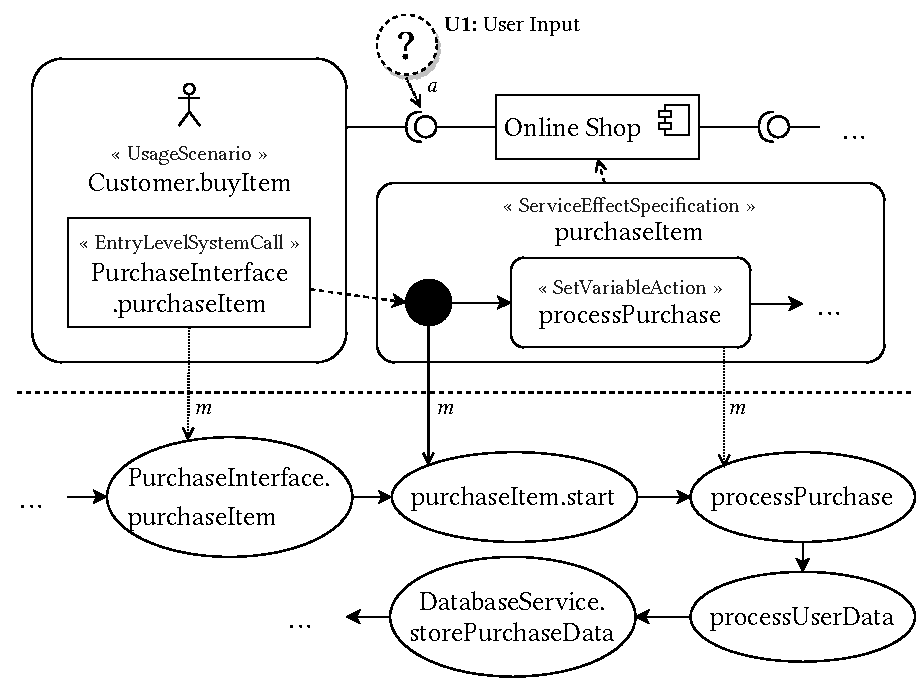
\includegraphics[width=0.9\linewidth]{figures/chapter6/impact-runningexample.pdf}
    \caption{Informal illustration of the propagation of an uncertainty source in the architectural model (top) and a \acf*{DFD} (bottom) using the annotation function a and the mapping function m.}
    \label{fig:impactanalysis:runningexample}
\end{figure}

To illustrate the propagation path of an uncertainty source, \autoref{fig:impactanalysis:runningexample} informally shows the propagation of Uncertainty \U{1}.
We chose this uncertainty source as it is annotated to the \emph{Customer} of the \emph{Online Shop} and thus has the longest path until it reaches a data sink.
For the sake of brevity, we leave out many details and focus only on the propagation path.
The full example can be found in our data set \cite{dataset}, and in \autoref{sec:appendix:impactset}.
Uncertainty \U{1} represents the user input and is annotated to a \emph{ProvidedDelegationConnector} called \emph{PurchaseInterface}.
It propagates to an \emph{EntryLevelSystemCall} in the \emph{UsageScenario} named \emph{Customer.buyItem} and to the \emph{StartAction} of a \ac{SEFF} in the architectural model.
The actions are mapped to \ac{DFD} nodes.
Afterward, the uncertainty is propagated in the \ac{DFD} until a sink is reached.
All \ac{DFD} nodes are part of the impact set of Uncertainty \U{1}.  


\subsection{Tool Support for Uncertainty Impact Analysis}

In the introduction of this chapter, we discussed the need for automated analyses to aid the software architectural design process.
Manual propagation of uncertainty is not feasible, especially in large systems of systems with hundreds of architectural elements or \ac{DFD} nodes \cite{hahner_architecture-based_2023}.
This need for automated analysis is also described in Problem \PR{2}{2}.

We realize the algorithms described in this chapter as part of our tooling \uia.
Here, we build on the Palladio tooling \cite{reussner_modeling_2016,reussner_palladio_2024} that offers a meta model, the \ac{PCM}, and graphical editor support.
Our Java-based open-source implementation of the propagation logic is integrated into the Eclipse-based tooling, and part of the data set \cite{dataset}.

\begin{figure}
\begin{lstlisting}[
    style=demo,
    caption={Shortened output of the uncertainty impact analysis showing the impact of Uncertainty U2.},
    label={lst:impactanalysis:result}
]
    Behavior Uncertainty Impact on SEFFActionSequenceElement with 
        ID _oEBNYDIXEe-m4c0ChzWfPg (represeting a SetVariableAction).
    Origin of this impact: Behavior Uncertainty annotated to 
        SetVariableAction "UserDataProcessing" (_oEBNYDIXEe-m4c0ChzWfPg).

    All affected elements (1):
    SEFFActionSequenceElement (UserDataProcessing, _oEBNYDIXEe-m4c0ChzWfPg)

    Impact set (1):
    0: SEFFActionSequenceElement (UserDataProcessing)
    CallingSEFFActionSequenceElement / calling (DatabaseStoreInventory)
    SEFFActionSequenceElement (Beginning updateInventory)
    SEFFActionSequenceElement (Ending updateInventory)
    CallingSEFFActionSequenceElement / returning (DatabaseStoreInventory)
    ...
\end{lstlisting}
\end{figure}

Here, we included many of the already discussed optimization strategies to speed up the propagation, e.g., by caching query results or using the extracted \ac{DFD} to filter affected architecture elements.
Using this approach, all propagation algorithms can be realized as \ac{DFS}, which is in $\mathcal{O}(V + E)$, where $V$ represents the \ac{DFD} nodes and $E$ represents the edges \cite{knuth_art_1997}.
Put simply, we test for each node whether or not it is affected by uncertainty, and then propagate the uncertainty along the data flow.

Software architects annotate uncertainty sources by calling the analysis interface and providing the element's identifier.
The analysis performs a type check to ensure the validity of the annotation and then propagates the uncertainty without requiring any further user interaction.
The result comprises the annotated elements, the affected elements in the \ac{PCM} model, and the complete impact set.
\autoref{lst:impactanalysis:result} shows an exemplary but shortened output of \uia for Uncertainty \U{2} with uncertainty type, annotation target, and analysis results.
The full output can be found in \autoref{sec:appendix:impactset}.
This output can be used to further enhance the display of the impact, e.g., by highlighting affected areas of \acp{DFD} in graphical viewers or editors \cite{boltz_extensible_2024}.

We also implemented additional processing to enhance the user experience.
As discussed in \autoref{sec:impactanalysis:dfdpropagation}, impact sets of uncertainty sources can be a subset of impact sets of other uncertainty sources.
In our running example, the impact set of \U{2} is a subset of the impact set of \U{1} because it affects a subgraph of the \ac{DAG} representing the user input's processing.
We identify such relations and only return the largest impact sets that are not subsets of another subset.
Formally speaking, the analysis yields an antichain \cite{diestel_graph_2017} with the partial order of the subset relation, in which all impact sets are pairwise incomparable.

\finding{The uncertainty impact analysis can be fully automated based on the \acf{PCM} and the existing tooling of the Palladio approach.
Propagating uncertainty requires minimal additional effort by software architects, as the analysis only requires annotating uncertainty sources.
}





\section{Addressing the Uncertainty Awareness Problem}%
\label{sec:impactanalysis:awareness}

Our approach to uncertainty impact analysis supports software architects in the early assessment of the impact of uncertainty on confidentiality.
However, it suffers from the \acf{UAP}, like many other uncertainty-aware analyses \cite{hezavehi_uncertainty_2021}.
As introduced in \autoref{sec:classification:identification}, the \ac{UAP} hinders the analysis of uncertainty due to the lack of knowledge about relevant uncertainty sources.
Failing the correct identification, classification, and annotation limits the validity of analysis results, as they can lack both precision and comprehensiveness.
In this section, we demonstrate how to tackle this problem regarding our uncertainty impact analysis.
We connect \arcen, which was introduced in \autoref{sec:classification:collaboration}, to our impact analysis tooling \uia.
This addresses Problem \PR{2}{3} and is a step toward end-to-end analysis approaches \cite{weyns_towards_2023}.

To tackle the \ac{UAP} in uncertainty impact analysis, we need to solve two underlying problems.
First, the analysis and its tooling must receive information about relevant uncertainty sources and their classification.
Second, software architects operating the analysis must become aware of potential sources and identify appropriate annotation targets.
Both problems arise before the automated analysis is performed.
Thus, we extend the uncertainty impact analysis by an additional identification step prior to the propagation.

After our tooling \uia has been initialized and all \ac{PCM} models are loaded, we request a current list of uncertainty sources from \arcen.
This is possible because \arcen provides the uncertainty source catalog in a machine-readable format, as presented in \autoref{sec:classification:collaboration}.
This catalog also includes the classification of each source, as shown with the underlying meta model in \autoref{fig:classification:identification:metamodel}.
Software architects use \arcen to identify relevant uncertainty sources.
As all uncertainty sources in the uncertainty source catalog have a unique identifier, they can provide this identifier to the extended impact analysis.
After resolving the uncertainty source and the classification category \emph{Architectural Element Type}, the analysis queries all \ac{PCM} models to identify matching annotations targets.
These are displayed to the software architects in an interactive interface.

\begin{figure}
\begin{lstlisting}[
    style=demo,
    caption={Exemplary interaction of a software architect with the extended uncertainty impact analysis.},
    label={lst:impactanalysis:awareness}
]
    Enter an id of an uncertainty to check for:
    > #48

    Select one of these elements.
    1) "OnPremiseServer" (_qvz80ITgEeywmO_IpTxeAg)
    2) "CloudServer" (_upfkIITgEeywmO_IpTxeAg)

    Enter line number:
    > 2

    Analysis completed. Result:
    ...
\end{lstlisting}
\end{figure}

\autoref{sec:impactanalysis:awareness} shows an exemplary interaction prior to the propagation of uncertainty.
In the running example, we have two \emph{ResourceContainers} that can be affected by uncertainty about the provider's trustworthiness (\U{4}), represented as uncertainty number 48 in \arcen.
After annotating this uncertainty source to the \emph{CloudServer}, the uncertainty impact analysis is executed.
The full result, including the impact set, is returned, similar to \autoref{lst:impactanalysis:result}.

This addresses the \ac{UAP} by providing software architects with a list of possible uncertainty sources to choose from.
Additionally, less expert knowledge about the classification is required as the interpretation is done automatically.
Last, the manual effort of searching the architectural model to identify potential elements to annotate with uncertainty is reduced.
In sum, this demonstrates the feasibility of extending an existing analysis, even without altering the core propagation algorithms.
We stress that other uncertainty-aware analyses \cite{hahner_model-based_2023,walter_architectural_2022,walter_architecture-based_2023} could similarly benefit from such extension.

\finding{By connecting the identification and classification of uncertainty to model-based uncertainty analysis, the \acf{UAP} can be addressed.
Although this does not fully resolve the challenge of unanticipated change, it reduces the severity.
Approaches like this represent a step toward the end-to-end analysis of uncertainty.}





\section{Uncertainty Propagation in Uncertainty Flow Diagrams}%
\label{sec:impactanalysis:ufd}

We conclude this chapter by discussing the generalization of the presented concepts to tackle related problems from the community of \acp{SAS} \cite{weyns_towards_2023}.
In the recent past, the \acf{UIP} has received increased attention \cite{camara_addressing_2022,camara_uncertainty_2022,weyns_towards_2023}.
This problem arises because uncertainties in software-intensive systems are rarely independent \cite{camara_uncertainty_2022}.
Addressing this problem goes beyond handling single uncertainty sources but poses additional challenges regarding modeling, analysis, and mitigation \cite{camara_addressing_2022}.
Handling the \ac{UIP} requires notations to represent and analyze the interaction of \emph{heterogeneous} uncertainty sources, i.e., uncertainty that differs in type and nature.
Additionally, this notation must support horizontal propagation in the same level of abstraction, and vertical propagation across abstraction levels.
This is also summarized in Problem \PR{2}{4}.

Uncertainty propagation has been identified early as a possible approach towards handling uncertainty interactions \cite{camara_addressing_2022}.
However, the few existing approaches tackling uncertainty propagation focus on \emph{homogeneous} uncertainties, i.e., uncertainties that are similar in nature, admit the same representations and are amenable to similar reasoning mechanisms \cite{camara_uncertainty_2024}.
In the following, we build on the knowledge about uncertainty propagation in \acp{DFD}, previously presented in this chapter.
We define a new notation called \acf{UFD} that enables the representation and propagation of heterogeneous uncertainty sources.
Thereby, we generalize the propagation concept introduced in this chapter and make a first step towards comprehensive modeling and analysis of the \ac{UIP}\footnote{When I presented the research about uncertainty propagation regarding confidentiality at SEAMS '23, I was asked by Danny Weyns about the application of these concepts to \acp{SAS}. My answer comprised the application of models at runtime and the integration into the analysis phase of \acs{MAPEK}. However, in hindsight, \acfp{UFD} would have been the perfect answer.}.

In our running example, we see an uncertainty interaction between Uncertainty \U{3} and \U{4}.
We discussed this interaction when we introduced the difference between primary and secondary uncertainty in \acp{DAG} in \autoref{sec:classification:dfd}.
If Uncertainty \U{3} resolves to a deployment location that is not in the cloud, Uncertainty \U{4} about the cloud provider has no effect.
Otherwise, the combination of both uncertainty sources is relevant.
This represents a simple uncertainty interaction where the outcome can be understood by investigating all possible scenarios.
However, other interactions could lead to results that go further and introduce new and unanticipated changes \cite{camara_addressing_2022,camara_uncertainty_2024}.
An example is Znn.com \cite{cheng_evaluating_2009}, where uncertainty about the sensor input interacts with the discretization of the input.
Here, the interaction of both uncertainties can lead to false adaption, although both uncertainty sources on their own would not have affected the system behavior \cite{camara_uncertainty_2024}.

\begin{figure}
    \centering
    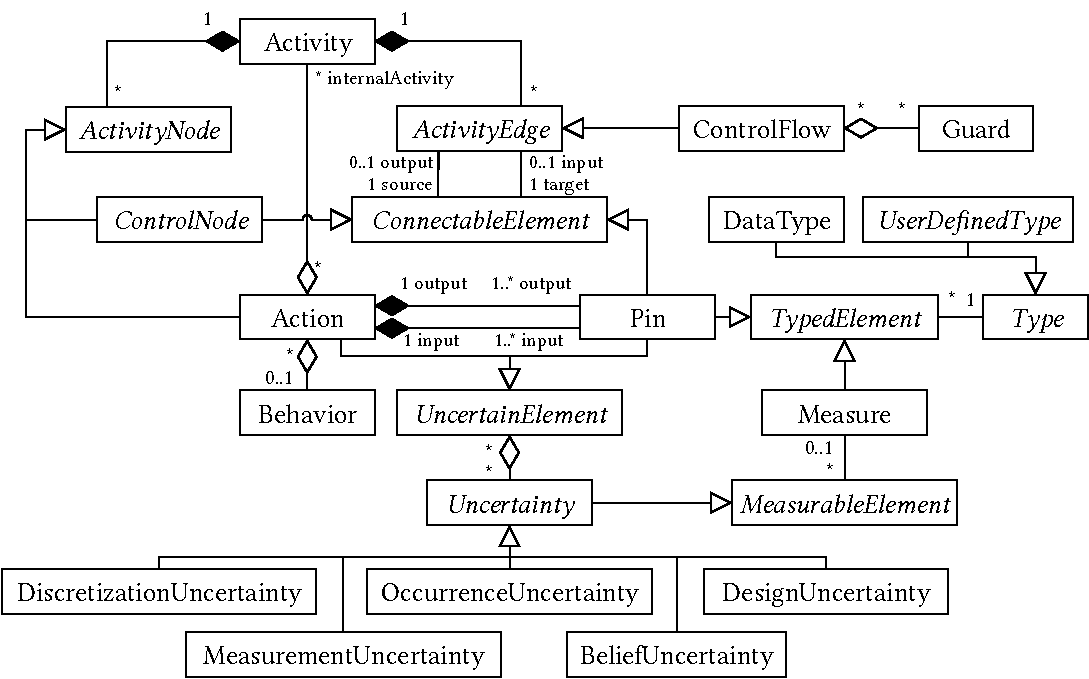
\includegraphics[width=\linewidth]{figures/chapter6/ufd.pdf}
    \caption{Simplified meta model of the \acf*{UFD} notation.}
    \label{fig:impactanalysis:ufd}
\end{figure}

\autoref{fig:impactanalysis:ufd} shows the simplified \ac{UFD} meta model \cite{camara_uncertainty_2024}.
This represents a simplified version of \acp{DFD} \cite{demarco_structure_1979} or \ac{UML} activity diagrams \cite{object_management_group_unified_2015}, extended with information about uncertainty, based on \ac{PSUM} \cite{PSUM}.
The top-level element is the \emph{Activity}, i.e., a graph whose nodes and edges are \emph{ActivityNodes} and \emph{ControlFlows}, respectively. 
The graph represents how the information flows through the computations performed by a program. 
\emph{Actions} represent behavior. 
\emph{Actions} are represented by squares with rounded corners and have \emph{Pins} (small white squares) that represent the types of input/output parameters. Each \emph{Pin} has a \emph{Type}.
\emph{Actions} may have an associated \emph{Behavior}, such as the invocation of a method that implements the behavior to transform the action's inputs into outputs.
This approach is similar to the unified modeling primitives \cite{seifermann_unified_2021}.

To enable hierarchical modeling and vertical uncertainty propagation, each \emph{Action} can also be refined by one or multiple \emph{Activities} that represent its inner workings. 
At the highest abstraction level, the whole system can be represented by a single node with input and output pins, i.e., a black box.
Either a \emph{Behavior} or a set of refining internal \emph{Activities} can be specified for an \emph{Action}, but not both.
It is also possible to specify multiple internal activities that represent alternatives.
This enables the expression of structural uncertainty as variations, which is common to represent design uncertainty \cite{troya_uncertainty_2021}.

A \emph{ControlFlow} is represented by a directed arrow that connects the outgoing \emph{Pin} of an \emph{Activity} with the incoming \emph{Pin} of another \emph{Activity}. 
\emph{ControlFlows} may include \emph{Guards} that have to be satisfied for the information to flow between the connected \emph{Pins}, or \emph{ControlNodes}. 
When more than one \emph{Guard} is specified, they all need to be satisfied for the \emph{ControlFlow} to take place.
\acp{UFD} enable the explicit representation of uncertainty, with the goal of dealing with the interactions between uncertainties that happen when making computations. 
\acp{UFD} allow the specification of individual uncertainties associated with \emph{Pins} or with \emph{Actions}. 
Each uncertainty can be of a different type.
This includes the common uncertainty types \emph{Measurement Uncertainty}, \emph{Discretization Uncertainty}, \emph{Occurrence Uncertainty}, \emph{Design Uncertainty}, and also \emph{Belief Uncertainty} \cite{troya_uncertainty_2021}.
Note that these types differ from the uncertainty types when only focusing on confidentiality.
Each uncertainty can have an associated \emph{Measure}, which also has a \emph{Type}. 
One way to assess a \emph{Measurement Uncertainty} is in terms of the accuracy of the measurement, which is normally expressed by means of a real number that represents the possible variation of the nominal value of the parameter, i.e., its estimated standard deviation. 
\emph{Belief Uncertainty} is normally expressed by a real number between 0 and 1 representing the likelihood that the stated fact is true, expressed as a probability.
Alternatively, uncertainty can be expressed by defining multiple \emph{Internal Activities} as a variation of the behavior of a single \emph{Action} which is used to express \emph{Design Uncertainty}.
This also enables the expression of additional uncertainty types if they can be denoted either quantitatively using an associated \emph{Measure} or structurally using alternative internal \emph{Activities}.

\begin{figure}
    \centering
    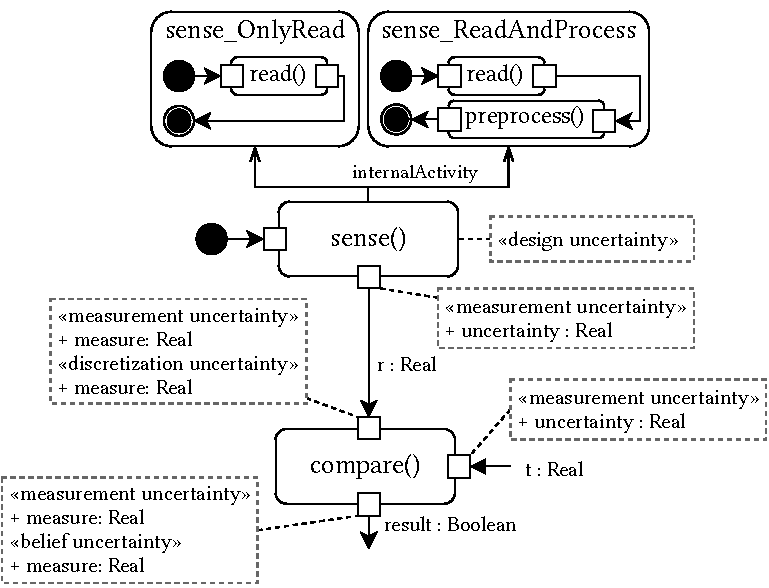
\includegraphics[width=0.8\linewidth]{figures/chapter6/ufd-example.pdf}
    \caption{An \acf*{UFD} showing heterogeneous uncertainty sources and hierarchical modeling.}
    \label{fig:impactanalysis:ufdexample}
\end{figure}

\autoref{fig:impactanalysis:ufdexample} shows an exemplary \ac{UFD}.
The \emph{compare} \emph{Action} compares a sensor value \emph{r} to a threshold \emph{t} to decide whether or not the adaption is triggered.
As described previously, both values are affected by \emph{Measurement Uncertainty}.
The input \emph{r} is additionally affected by \emph{Discretization Uncertainty}, and the uncertain correctness of the \emph{result} is thus subject to \emph{Belief Uncertainty}.
These uncertainties are attached to the matching \emph{Pins} and can be expressed using \emph{Measures}, e.g., the degree of belief, or the variation of the measurement \cite{PSUM}.
Additionally, this example shows \emph{Design Uncertainty} in the \emph{sense} \emph{Action}.
Here, two versions are possible, depending on whether additional preprocessing is used.
This can affect the \emph{Measurement Uncertainty} in \emph{r} and is represented using \emph{Internal Activities}.

In sum, this notation enables the expression of heterogeneous uncertainty sources and their propagation, both horizontally and vertically.
Thereby, \acp{UFD} are still close to the unified modeling primitives \cite{seifermann_unified_2021} or \acp{DFD}\footnote{This research started at the 2023 Bertinoro research seminar on uncertainty in \acp{SAS}. Our group consisted of Javier Camara, Diego Perez-Palacin, Antonio Vallecillo, Maribel Acosta, Nelly Bencomo, Radu Calinescu, Simos Gerasimou, and myself. After discussing the \acf{UIP} for days, we were surprised how concise \acfp{UFD} can be.}.
The propagation of uncertainty in \acp{UFD} is similar to the propagation in \acp{DFD}, i.e., following all edges of a node until a sink is reached.
Although \acp{UFD} are a promising approach to generalize the propagation concept to analyze more than confidentiality, this still represents an early proposal \cite{weyns_towards_2023}.
Future research in this direction is required to create comprehensive and tool-supported modeling and analysis approaches to address the \ac{UIP}.





\section{Assumptions and Limitations}%
\label{sec:impactanalysis:limitations}

In this section, we discuss the assumptions and limitations of the different approaches to uncertainty propagation and impact analysis presented in this chapter.
We also provide our reasoning on whether limitations can become critical when applying the approaches.

\paragraph{Using data flow diagrams}
We use \acp{DFD} to investigate confidentiality as proposed by other work \cite{seifermann_detecting_2022,sion_security_2020,schneider_how_2024}.
Although this simplifies the propagation algorithms and provides a widely used and well-known foundation for our work, it limits the generalizability.
The uncertainty propagation in \acp{DFD} is only defined for this notation and the architectural propagation yields elements that can be represented by \ac{DFD} elements.
This limitation is similar to the limitation of focusing on confidentiality, discussed in \autoref{sec:classification:limitations}.
However, we argue that our findings about the propagation of uncertainty are at least partially generalizable, as shown with the definition of \acp{UFD} in \autoref{sec:impactanalysis:ufd}.

\paragraph{Choice of architectural description language}
We choose the \ac{ADL} \ac{PCM} to define our algorithms for the architectural uncertainty impact analysis.
The \ac{PCM} is well known \cite{sobhy_evaluation_2021} and easy to extend.
Nevertheless, this limits the generalizability to other descriptions of software architecture like \ac{UML} diagrams \cite{object_management_group_unified_2015}.
We argue that the foundation of the propagation, our classification defined in \autoref{ch:classification}, is general enough to also define propagation rules for other \acp{ADL}.
Additionally, the architectural impact analysis is limited by the specified annotations targets of uncertainty sources.
Here, the same argument can be made, that extending the analysis to other architectural elements based on the provided propagation algorithms is possible and should require reasonable effort.

\paragraph{Correctness of propagation rules and of the mapping}
We assume the correctness of the propagation rules for architecture-based change impact analysis from the \ac{KAMP} approach \cite{rostami_architecture-based_2015,rostami_architecture-based_2017,busch_architecture-based_2020}.
We also assume the appropriateness of the mapping from the \ac{PCM} to \acp{DFD} \cite{seifermann_data-driven_2019,seifermann_detecting_2022,seifermann_architectural_2022}.
Erroneous propagation or mapping rules could decrease the validity of the results of our uncertainty impact analysis.
However, both represent well-validated and well-published research approaches.

\paragraph{Overestimation of the impact set}
Our uncertainty impact analysis overestimates the uncertainty impact set, as discussed in \autoref{sec:impactanalysis:pcmpropagation}.
This is intentional as we argue that a high recall is more important than a high precision in the early assessment of uncertainty \cite{hahner_architecture-based_2023}.
However, the usefulness of the impact set depends on the analyzed architectural model.
Architectural models with only a few independent data flows are more likely to yield imprecise results, as the majority of the software system would be affected by the uncertainty sources.
We argue that realistic software systems comprise enough independent data flows \cite{schneider_microsecend_2023} to apply the analysis with satisfying results.

\paragraph{Propagating uncertainty until a sink is reached}
The uncertainty impact analysis in \acp{DFD} propagates uncertainty starting at a specified node by following all outgoing data flows until a sink is reached.
Similarly to the architectural uncertainty impact analysis, this overestimates the impact of uncertainty.
For instance, if at one point in the \ac{DFD}, every data flow is encrypted, this limits the impact of previous uncertainties about the encryption.
This is comparable to approaches to reduce uncertainty during operation, e.g., robots that use visual markers to reduce the uncertainty about their location \cite{camara_software_2020}.
However, we ignore such uncertainty reduction and propagate uncertainty until the end of each data flow.
Considering such interdependence of uncertainty and confidentiality would increase the precision but also require to already consider confidentiality requirements in the uncertainty propagation, which would increase the manual modeling effort.
Nevertheless, this represents an interesting direction for future research.

\paragraph{Propagating unknown uncertainty sources}
Similarly to the limitation of classifying unknown uncertainty sources discussed in \autoref{sec:classification:limitations}, we can also not propagate them.
Software architects have to be at least aware of an uncertainty source in order to annotate and to propagate the uncertainty.
The connection of our identification approach, presented in \autoref{sec:classification:identification}, to our uncertainty impact analysis can partially address this limitation.
Providing software architects with an uncertainty source catalog that can be propagated reduces the impact of the unknown.
Nevertheless, we cannot assume that all required information is available as the underlying challenge of unanticipated change remains.

\paragraph{Querying annotation targets}
By connecting our identification approach, presented in \autoref{sec:classification:identification}, to our uncertainty impact analysis, we simplify the annotation of uncertainty sources.
However, the querying of elements of the software architecture that match a selected uncertainty source only considers the category \emph{Architectural Element Type}.
Including further categories like the \emph{Location} could enhance the precision of annotations targets recommended to the software architect, but could also cause false negatives.
Further research is required to enhance the recommendation and explanation of uncertainty \cite{bersani_conceptual_2023}.
We argue that our initial filter already greatly reduces the number of matching uncertainty sources and is thus helpful.

\paragraph{Solving the uncertainty interaction problem}
\acp{UFD} represent a notation to express and propagate different uncertainty types to tackle the \ac{UIP}.
Nevertheless, this does not fully solve the challenge of uncertainty interactions \cite{camara_addressing_2022}.
Challenges regarding tool-supported modeling, the transformation between different notions, and automated analysis remain.
However, \acp{UFD} represent a first step for further research in this direction \cite{camara_uncertainty_2024,weyns_towards_2023}.





\section{Summary and Outlook}%
\label{sec:impactanalysis:summary}

In this chapter, we presented different approaches to uncertainty propagation to define an \emph{uncertainty impact analysis} regarding confidentiality.
This represents our second Contribution \C{2} and provides an answer to \RQ{2}.

First, we discussed the representation of uncertainty in architectural models to address Problem \PR{2}{1}.
We presented a distinction between uncertainty \emph{sources} and their \emph{impact} and related this terminology to architectural models and \acp{DFD}.
We introduced a meta model of \acp{DFD} under uncertainty that relates the different uncertainty impact types to \ac{DFD} elements.
Last, we discussed where uncertainty sources can be annotated within the \ac{PCM} to enable architectural uncertainty propagation.

To address Problem \PR{2}{2}, we combined uncertainty propagation in architectural models with propagation along the data flow in \acp{DFD}.
First, we discussed the relation of architecture-based change impact analysis \cite{busch_architecture-based_2020} and uncertainty impact analysis.
Afterward, we presented propagation algorithms for each uncertainty type described in our classification, introduced in \autoref{ch:classification}.
We described how to map the propagation results to \acp{DFD} and to further propagate uncertainty following the flow of data.
Hereby, we also provided a formal foundation based on \acp{DAG} and induced subgraphs that represent the impact of uncertainty.
We explained this impact analysis using our running example and introduced our tooling \uia to automate uncertainty impact analysis.

Problem \PR{2}{3} describes the \ac{UAP} regarding uncertainty impact analysis, i.e., the lack of knowledge about uncertainty sources to propagate.
We addressed this problem by combining the identification approach, introduced in \autoref{sec:classification:identification}, with the uncertainty impact analysis.
Regarding the tool support, this meant combining \arcen with \uia.
The resulting analysis simplifies both the identification of relevant uncertainty sources and the identification of annotation targets.

Last, we generalized the findings on the propagation of uncertainty in \acp{DFD} to better understand the \ac{UIP}, as discussed with Problem \PR{2}{4}.
To analyze uncertainty interactions, we defined the notation of \acp{UFD} that can express heterogeneous uncertainty sources and support both horizontal and vertical propagation of uncertainty. 
This notation provides a foundation for further modeling and analysis approaches to tackle the \ac{UIP}.

\RQ{2} asked about the propagation of previously classified uncertainty sources to predict their impact on confidentiality.
We observe that a comprehensive approach requires both the propagation in architectural models and \acp{DFD}.
Our answer thus comprises means for modeling uncertainty in both representations and propagation algorithms for architectural models based on the \ac{PCM} and also \acp{DFD}.
To connect the resulting uncertainty impact analysis regarding confidentiality to classified uncertainty sources, we discussed the connection of this approach to uncertainty source catalogs.
In sum, this enables software architects to assess the impact of uncertainty in existing architectural models with regard to confidentiality.

The central benefit of early impact analysis is cost reduction due to the early detection of potential problems \cite{boehm_software_2001}.
Here, uncertainty impact analysis can be applied even earlier than design time confidentiality analysis \cite{seifermann_detecting_2022}, because propagating uncertainty does not require details about data processing or confidentiality requirements.
Nevertheless, propagating uncertainty helps software architects in mitigating uncertainty early \cite{acosta_uncertainty_2022}.
Architecture models can be annotated with uncertainty sources from existing collections \cite{hahner_classification_2023} which helps in the documentation and to raise awareness.
The analysis helps predict and mitigate confidentiality violations.
Using a confidentiality analysis for this purpose would require software architects to understand and model the impact of uncertainty manually which requires more effort and expertise.
Note that we do not state that uncertainty impact analysis replaces the need for confidentiality analysis.
However, it can be used for an initial, coarse-grained assessment, as discussed in our procedure, introduced in \autoref{sec:overview:procedure}.
Last, the calculated models of our analysis can also be used for regression testing or to handle uncertainty at runtime \cite{derakhshanmanesh_model-integrating_2019}.

To conclude, we want to briefly discuss another application of uncertainty propagation.
We investigated uncertainty in coupled models \cite{acosta_uncertainty_2022}, e.g., in the automotive domain, where experts from different areas work together.
They require different views, e.g., a system architecture, an electrical topology with hardware components, or simulation results.
To keep these views consistent, the underlying models are coupled using consistency specifications \cite{klare_enabling_2021}.
Based on the classification of uncertainty in \acf{CPS}, we derived the category \emph{Locus} that is similar to \emph{Architectural Element Type}.
This category also defines where uncertainty can be annotated and how it propagates through the models.
Although this is based on consistency specifications and not architectural change impact analysis, uncertainty propagation can be applied and helps in mitigation.

\finding{Interpreting uncertainty as unanticipated change enables its propagation not only based on change impact analysis, but also using other methods of change propagation, such as consistency specifications.
Uncertainty propagation is a powerful technique to better understand the effect of unanticipated changes, or even to detect new uncertainty, e.g., due to uncertainty interactions.}

We will revisit uncertainty propagation and interaction in \readingpath{ch:confidentialityanalysis}.
There, we present different approaches to confidentiality analysis under uncertainty that build on the findings of this chapter.
Especially the concept of uncertainty interactions helps in optimizing the uncertainty-aware analysis of confidentiality.
Both the uncertainty impact analysis and confidentiality analysis under uncertainty are based on our uncertainty classification, presented in \readingpath{ch:classification}.
An overview of the procedure that connects all of these steps is given in \readingpath{ch:overview}.
Last, \readingpath{ch:evaluation} presents the evaluation of all contributions, including the uncertainty impact analysis presented in this chapter.





\section{In Simpler Words}%
\label{sec:impactanalysis:simple}

Uncertainty has many definitions.
Some define uncertainty as a lack of knowledge about a software system and its environment, while others refer to uncertainty as unanticipated change, i.e., changes in a software system that have not been foreseen.
Our goal in this chapter is to define an \emph{uncertainty impact analysis}.
When experts become aware of an uncertainty source, they want to better understand its potential impact.
Not all uncertainty sources have severely bad effects, many do not even affect confidentiality.
Our classification, defined in \autoref{ch:classification}, helps in an early inspection of an uncertainty source.
However, to really understand the impact, they need to look at the software system, and analyze its software architecture and data flows.
Our contribution in this chapter supports the experts in this activity and even automates the majority of it.

We call the core idea of uncertainty impact analysis \emph{uncertainty propagation}---both are so closely related that we even use them synonymously.
Propagation refers to the uncertainty being forwarded or transmitted through a software system.
For instance, if the data processing of a system part is uncertain, this may also affect other system parts where the data flows.
The uncertainty of the data processing propagates through the software system.
Here, we build on the finding that uncertainty can be understood as unanticipated change, as described above.
Other researchers defined architecture-based change impact analysis that propagates change through software systems.
For instance, if we rename a signature in an interface, we must also rename the calls to this signature in all methods.
This propagation, from a changed element to other elements that also have to adapt, is called change propagation, and the result of such propagation is called \emph{impact set}.
Change impact analysis can estimate the impact set---and we build on this to estimate the impact set of uncertainty.

We define many algorithms to propagate uncertainty within the software architecture.
These algorithms precisely describe which elements of a software architecture can be indirectly affected by an uncertainty source.
Here, we build on the classification category \emph{Architectural Element Type}, presented in \autoref{ch:classification}.
Afterward, we move from the software architecture to \acfp{DFD} and propagate the impact of uncertainty along all potentially affected data flows.
This helps us avoid overlooking potential confidentiality violations due to impacted data flowing to another part of the software system.
Remember the example of the data processing that could cause problems somewhere else.
We express the final impact set using the \ac{DFD} of the software system.

Building on this analysis, we describe several extensions.
For example, we relate the previously discussed awareness problem of uncertainty to the analysis.
Although our impact analysis helps to better understand the effect of uncertainty, it requires experts to be aware of uncertainty sources.
We address this limitation by providing them with uncertainty source catalogs, which can be propagated.
Last, we discuss the generalization of our uncertainty propagation.
We propose \acfp{UFD} to represent different uncertainty types in a single diagram type.
This notation also helps to better understand \emph{uncertainty interactions}, which have been introduced in \autoref{ch:classification}.
In the future, approaches like this will hopefully be helpful in many related research directions.

\chapter{Uncertainty-Aware Data Flow Analysis to Identify Confidentiality Violations}%
\label{ch:confidentialityanalysis}%
 

In this chapter, we present the third Contribution \C{3}.
This contribution covers the last activity of the procedure shown in \autoref{sec:overview:procedure}, the confidentiality analysis with respect to uncertainty.
We discuss the representation of uncertainty as a first-class entity in data flow analysis and introduce four approaches for uncertainty-aware confidentiality analysis.

Software systems are becoming increasingly complex, e.g., in Industry 4.0 \cite{boltz_context-based_2020} or automotive systems \cite{acosta_uncertainty_2022}.
As stated previously, ensuring security-related quality properties like confidentiality becomes a major challenge.
Violations cannot only have legal consequences \cite{isaak_user_2018} but also affect user acceptance \cite{weisbaum_trust_2018}.
As proposed by \emph{Privacy by Design} \cite{schaar_privacy_2010}, confidentiality should be considered early to avoid costly repairs \cite{boehm_software_2001}.
This can also seen with the new \enquote{Insecure Design} category from the \ac{OWASP} Top 10 \cite{OWASPTop10} list, which contains the top 10 categories of security problems for web applications. 

This problem has been addressed with design time confidentiality analysis.
By analyzing data flows \cite{seifermann_detecting_2022} or potential attack paths \cite{walter_architectural_2022-1,walter_architecture-based_2023-1} in modeled software architectures, confidentiality requirements \cite{hahner_modeling_2021} can be evaluated early.
We discussed these approaches in previous chapters, especially in \autoref{ch:impactanalysis}.
There, we built on the transformation from the \acf{ADL} \acf{PCM} to \acfp{DFD} in order to propagate uncertainty regarding confidentiality.
This transformation originates from an architecture-based data flow analysis to identify confidentiality violations already at design time \cite{seifermann_data-driven_2019,seifermann_detecting_2022,seifermann_architectural_2022}.
Based on an architectural description of the software system, violations of provided confidentiality requirements \cite{hahner_modeling_2021} can be identified.
This involves the model-based propagation of characteristics within the software architecture, which describe the flowing data and its properties regarding confidentiality.
In sum, these approaches enable software architects to assess the confidentiality of software systems.

However, in early development and in complex systems of systems, uncertainty exists about the software architecture and its environment \cite{acosta_uncertainty_2022}.
Our running example from \autoref{ch:runningexample} shows multiple uncertainty sources, e.g., user input (\U{1}), data processing (\U{2}), or deployment (\U{3}).
When ignored, these uncertainties affect both the precision and comprehensiveness of the results of confidentiality analysis \cite{hahner_classification_2023,hahner_dealing_2021,hahner_architectural_2021}.
The lack of information reduces the quality of the model's representation of the software system. 
This results in less accurate or even wrong predictions, made on the basis of the model. 
Although uncertainty-aware analyses of software architectures exist \cite{esfahani_guidearch_2013}, they usually focus on other quality properties like performance \cite{sobhy_evaluation_2021}.

To address this limitation, we present multiple approaches to architectural confidentiality analysis under uncertainty.
We build on the findings about \acp{DFD} and uncertainty from the previous chapters to define data flow analyses that identify violations of confidentiality requirements with respect to uncertainty.
Taking known uncertainty into account helps in making more comprehensive statements about a software system's confidentiality.
The handling of uncertainty can either be included as part of the analysis in a white-box manner or delegated to an uncertainty-aware framework \cite{acosta_uncertainty_2022}.
Here, we keep the architectural abstraction to enable design time analysis.
Similarly to the previous chapter, we also propose automated analysis and tool-supported modeling as \enquote{detecting confidentiality issues manually is not feasible} \cite{seifermann_data-driven_2019}.

In sum, to define uncertainty-aware data flow analysis, advances both in modeling and analysis of confidentiality and uncertainty are required.
As proposed by \textcite{garlan_software_2010}, we thereby include uncertainty as a first-class concern in the system design.
We present two approaches for confidentiality analysis that are tailored to single uncertainty types, e.g., environmental, or structural uncertainty, as well as two uncertainty type-agnostic approaches.
We also discuss common challenges and solutions in representing uncertainty in data flow analysis.
We summarize this research concern of uncertainty-aware data flow analysis regarding confidentiality in the third research question:

\RQthree

The remainder of this chapter is structured as follows:
First, we discuss the problem statement.
We then introduce a framework for architectural data flow analysis.
This framework builds on the architecture-based data flow analysis of \textcite{seifermann_architectural_2022,seifermann_identifying_2021}, but extends and simplifies both the modeling and the analysis.
It lays the foundation for the further analysis approaches presented in this section.
Afterward, we discuss how to represent uncertainty in data flow analysis.
Depending on the approach and the use of existing information, different statements about confidentiality and uncertainty can be derived.
Building on this, we present two approaches for uncertainty type-specific data flow analysis.
The first uses fuzzy inference \cite{klir_fuzzy_1995} together with data flow analysis to consider environment uncertainty.
The second extends the architectural optimization approach PerOpteryx \cite{koziolek_peropteryx_2011,koziolek_automated_2011} to consider the relation of structural uncertainty and confidentiality.
Additionally, we present an approach to tracing uncertainty in data flow analysis and an uncertainty type-agnostic approach to data flow analysis.
Last, we discuss the complexity of the different uncertainty-aware data flow analysis approaches.
We close the chapter by presenting assumptions and limitations and giving a summary.

\ownpublications{
\fancycite{boltz_handling_2022},
\fancycite{walter_architectural_2022},
\fancycite{hahner_model-based_2023},\linebreak
\fancycite{boltz_extensible_2024}
}





\section{Problem Statement}%
\label{sec:confidentialityanalysis:problem}

We summarize the problems \textbf{P1} -- \textbf{P3} addressed by Contribution \C{3}.
Finding solutions to these problems helps to provide a comprehensive answer to \RQ{3}.

\paragraph{P1: Extending data flow analysis to represent uncertainty}\label{p:3:1}
To consider uncertainty in architectural data flow analysis, we first require an extensible framework for data flow analysis \cite{boltz_extensible_2024}.
This framework lays the foundations for any type of uncertainty-aware data flow analysis that goes beyond black-box approaches \cite{walter_architectural_2022}.
By black-box approaches, we mean approaches to confidentiality analysis that do not consider uncertainty as a first-class entity but encapsulate an existing analysis into an uncertainty-aware framework.
Additionally, we need to understand how uncertainty can be represented in confidentiality analysis \cite{hahner_model-based_2023}.
This requires relating previous findings on modeling and propagating uncertainty in architectural models to data flow analysis.
We stress that there is no single solution to this problem but various solutions that exhibit different benefits and drawbacks.
A common baseline is envisaged to understand their characteristics and applications.

\paragraph{P2: Data flow analysis tailored to specific uncertaint types}\label{p:3:2}
To better understand the relation of uncertainty and confidentiality on architectural abstraction, we first strive to define architecture-based data flow analysis tailored for specific uncertainty types.
Here, we focus on uncertainty types that are common in software architectures.
This includes structural uncertainty due to \acfp{ADD} \cite{walter_architectural_2022,jansen_software_2005} and also environmental uncertainty that can indirectly affect confidentiality, e.g., due to access control decisions under uncertainty \cite{boltz_handling_2022,bures_capturing_2020}.
Although such focused analysis approaches are unable to analyze all uncertainty types that can affect confidentiality, they still provide precise results regarding single uncertainty types, especially compared to uncertainty-unaware confidentially analysis \cite{seifermann_architectural_2022}.
Additionally, they present an important step towards uncertainty type-agnostic data flow analysis \cite{hahner_model-based_2023}.

\paragraph{P3: Uncertainty type-agnostic data flow analysis} \label{p:3:3}
Ultimately, a comprehensive approach is required to analyze all uncertainty types that are relevant regarding confidentiality.
Building on the findings from \PR{3}{1} and \PR{3}{2}, this approach shall be able to handle all uncertainty types described in the uncertainty classification, presented in \autoref{ch:classification}.
This uncertainty type-agnostic approach needs modeling support for expressing uncertainty in architectural models that goes beyond the annotation of uncertainty sources required for uncertainty impact analysis, discussed in \autoref{ch:impactanalysis}.
A common approach to expressing uncertainty in architectural models is modeling variation scenarios \cite{troya_uncertainty_2021,walter_architecture-based_2023}.
However, analyzing variations---and especially combinations of variations---can quickly jeopardize the scalability \cite{walter_context-based_2023,walter_architecture-based_2023-1}.
Building on previous findings regarding the \acf{UIP} in \acp{DFD} can reduce the analysis complexity.





\section{A Framework for Architectural Data Flow Analysis}%
\label{sec:confidentialityanalysis:framework}

In this section, we build on an approach for architecture-based data flow analysis \cite{seifermann_architectural_2016,seifermann_data-driven_2019,seifermann_detecting_2022,seifermann_unified_2021,seifermann_architectural_2022} to present our extensible framework for architectural data flow analysis \cite{boltz_extensible_2024}.
This lays the foundation for further analysis approaches---which are not limited to uncertainty only---and also addresses Problem \PR{3}{1}.

In general, there are two ways to approach uncertainty-aware analysis \cite{acosta_uncertainty_2022,perez-palacin_dealing_2014}.
We use the common differentiation between \emph{white-box} analysis and \emph{black-box} analysis composition \cite{taghavi_survey_2023,heinrich_composing_2021}.
A black-box approach extends an analysis without knowing about the implementation details of the analysis and only uses its interfaces.
A white-box approach can use the internal details and data structures for the composition.
Both approaches have benefits and drawbacks, e.g., regarding expressiveness and maintainability.
Regarding uncertainty, we favor white-box analysis approaches as they enable the representation of uncertainty as a first-class entity within the analysis \cite{garlan_software_2010}.
However, this does not imply that black-box approaches are not feasible \cite{walter_architectural_2022}.
To enable white-box analysis, we require an extensible and stable analysis framework.

Regarding the architectural data flow analysis, the original Prolog-based implementation of \textcite{seifermann_architectural_2022} was hard to maintain and had a high resource demand, which severely limits the applicability for large software systems.
Although the analysis already used a model of a \ac{DFD} \cite{demarco_structure_1979} as an intermediate representation, it did not continue to follow the idea of using \acp{DFD} as the primary analysis artifact. 
With appropriate tool support, \acp{DFD} represent a powerful and commonly used mechanism for threat analysis \cite{bernsmed_adopting_2022} that helps in correctly identifying security-related issues \cite{schneider_how_2024}.
Thus, we revisited all aspects of the analysis like the transformation of \ac{PCM} models to \acp{DFD}, and the label propagation, and also reimplemented the analysis from scratch \cite{schwickerath_tool-supported_2023}.
This results in a more scalable and also easier-to-extend analysis framework \cite{boltz_extensible_2024}.
Additionally, the focus on \acp{DFD} as the primary analysis artifact simplifies the connection to uncertainty, as discussed in \autoref{sec:classification:dfd}. 
We introduced some of the underlying concepts already in \autoref{ch:foundations}.
For the scope of this work, we summarize the internal data structures and the analysis procedure and refer to our publications for more details \cite{schwickerath_tool-supported_2023,boltz_extensible_2024,hahner_modeling_2021}.


\subsection{Representing Data Flows in Data Flow Analysis}

As discussed in \autoref{sec:classification:dfd}, \acp{DFD} can be represented as \acfp{DAG}.
Using a simple graph structure simplifies the reasoning and the automated analysis regarding confidentiality.
We support the transformation of \acp{DFD}, which are based on the unified modeling primitives \cite{seifermann_unified_2021}, and also of \ac{PCM} models \cite{reussner_modeling_2016} to \acp{DAG}.
The former enables the manual definition of \acp{DFD}, and the latter extends the integration of architectural models in the data flow analysis \cite{seifermann_data-driven_2019}.

To represent data flows and their relations in \acp{DAG}, we use the notion of a \acf{TFG}.
Flow graphs represent the flow from one source to one or multiple sinks \cite{knuth_art_1997}.
However, regarding confidentiality, we are more interested in the relations of data flows from multiple sources to a single sink.
An example is the joint flow of multiple sensitive data flows into a single sink, e.g., pseudonymized data flowing together with information about the relation of the data to its originating users, which could violate confidentiality.
We use these transposed semantics of a flow graph, thus creating \acp{TFG}.
Reasoning about multiple, smaller \acp{TFG} instead of one large \ac{DAG} provides further benefits.
It represents a divide and conquer approach, as the data flows represented by \acp{TFG} are independent and can thus be analyzed independently \cite{seifermann_architectural_2022}.
This simplifies the analysis and increases its scalability \cite{schwickerath_tool-supported_2023}.
It is also more intuitive because confidentiality analysis represents identifying critical data flows to a single destination, i.e., critical \acp{TFG}.

\begin{figure}
    \centering
    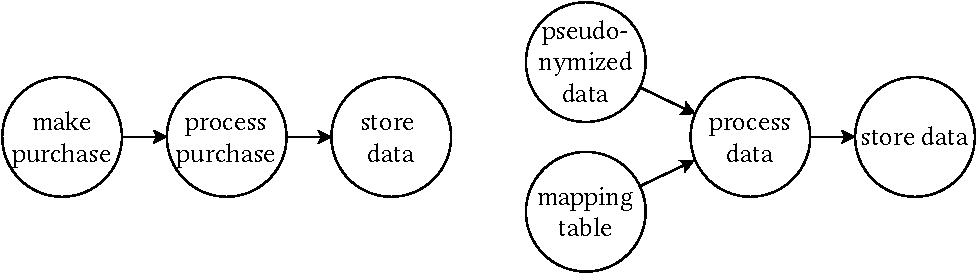
\includegraphics[width=\linewidth]{figures/chapter7/tfg.pdf}
    \caption{Two \acfp*{TFG} representing two independent data flows.}
    \label{fig:confidentialityanalysis:tfg}
\end{figure}

\autoref{fig:confidentialityanalysis:tfg} shows two \acp{TFG}.
The left \ac{TFG} represents a simple data flow from the running example presented in \autoref{ch:runningexample}.
The right \ac{TFG} represents the combination of data flows from two sources into a single sink, as discussed above with pseudonymized data.
We can see, that the data flows in \acp{TFG} inherit all properties from \ac{DAG}, i.e., being irreflexive, asymmetric, and transitive.
Additionally, starting from the single sink, all other vertices are reachable without cycles.
We can also see, that the partition in multiple, independent \acp{TFG} simplifies the reasoning.
In the example shown in \autoref{fig:confidentialityanalysis:tfg}, both \emph{store data} processes could be represented by the same call to a data base.
However, both data flows are independent, represent different data types and data processing, and also could cause different confidentiality violations.
For instance, storing data without encryption could violate the confidentiality in the \emph{store data} process in the left \ac{TFG}, while \emph{process data} could violate the confidentiality due to a broken pseudonymization in the right \ac{TFG}.

\finding{\acfp{TFG} show independent data flows of a \acf{DAG}.
Following the principle of divide and conquer, this simplifies reasoning about the variety of data flows in a system.}

To enable confidentiality analysis, we connect the concept of \acp{DAG} and \acp{TFG} to the unified modeling primitives \cite{seifermann_unified_2021}, introduced in \autoref{sec:foundations:dfd}.
Here, \emph{Nodes} and \emph{Flows} can be represented directly by vertices and edges, respectively.
Additionally, vertices can be annotated with \emph{Labels} to represent their characteristics regarding confidentiality, called \emph{node labels}.
Examples of such labels are the deployment location or the role of a user.
The \emph{Behavior} of a \emph{Node}, represented by one or multiple \emph{Assignments} can also be directly mapped to the vertices of a \ac{TFG}.
\emph{Assignments} can change the characteristics of flowing data, represented by \emph{data labels}.
For example, the behavior of the \emph{process purchase} vertex in \autoref{fig:confidentialityanalysis:tfg} could include setting an \emph{encrypted} label to represent the encryption of all data flows.
Last, \emph{Pins} are not directly represented in \acp{TFG} but influence their construction.
For instance, multiple \emph{Flows} out of a single \emph{Pin} represent alternatives that yield a \ac{TFG} for each alternative flow.
Again, for the scope of this work, we do not detail the transformation of \acp{DFD} to \acp{TFG}, but refer to the original publications \cite{seifermann_detecting_2022,boltz_extensible_2024}.

\begin{figure}
    \centering
    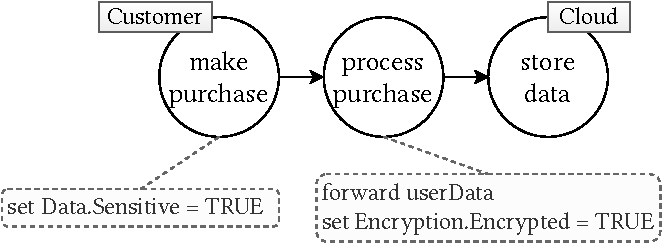
\includegraphics[width=0.7\linewidth]{figures/chapter7/annotatedtfg.pdf}
    \caption{A simple \acf*{TFG}, annotated with node labels and node behaviors.}
    \label{fig:confidentialityanalysis:annotatedtfg}
\end{figure}

\autoref{fig:confidentialityanalysis:annotatedtfg} shows the left \ac{TFG} from \autoref{fig:confidentialityanalysis:tfg}, annotated with node labels and behaviors, following the notation of the data flow analysis framework \cite{boltz_extensible_2024}.
The exemplary \emph{node labels} show which vertices represent functionality of the \emph{Customer}, or of components deployed in the \emph{Cloud}.
Note that there is no general rule on which characteristics can and should be represented by node labels---any information, that can be relevant for analyzing confidentiality, can be included within the model \cite{seifermann_architectural_2022}.
The exemplary node behaviors show how the \emph{data labels} can be altered.
First, the \emph{make purchase} vertex sets the label \emph{Data.Sensitive}.
Then, this label is forwarded in the \emph{process purchase} vertex, where also the label \emph{Encryption.Encrypted} is added.
Both labels flow to the \emph{store data} vertex.
In natural language, this simple \ac{TFG} represents sensitive user data that flows from a user into a database that is deployed in the cloud, while being encrypted first.
This notion simplifies reasoning about data flows regarding confidentiality and can also be applied to large \ac{DFD} with thousands of nodes \cite{schwickerath_tool-supported_2023}.

Confidentiality requirements can be formulated in the form of data flow constraints \cite{hahner_modeling_2021}.
These constraints restrict selected \emph{data labels} to never flow to selected \emph{node labels}.
In the example shown in \autoref{fig:confidentialityanalysis:annotatedtfg}, an exemplary data flow constraint could be that there shall not be a data flow of sensitive but unencrypted data to the cloud.
Due to the encryption in the vertex \emph{process purchase}, this data flow constraint is satisfied.
Thus, this constraint would not cause a confidentiality violation.
More complex constraints that consider the multiple flows and their properties are also possible \cite{hahner_modeling_2021,boltz_extensible_2024}.

\finding{\acfp{TFG} can be annotated with characteristics that represent system properties relevant for confidentiality analysis.
These characteristics comprise node labels, which are annotated to vertices, and data labels, which are altered by a node's behavior.
Confidentiality requirements can be represented as data flow constraints that compare node and data labels.}

Although the manual modeling of \acp{DAG} with confidentiality characteristics is possible \cite{boltz_extensible_2024}, we focus on the automated extraction of \acp{DAG} from \ac{PCM} models.
We introduced this extraction in \autoref{sec:impactanalysis:pcmpropagation}.
For instance, \emph{ExternalCallAction}, \emph{SetVariableAction}, and \emph{EntryLevelSystemCalls} are represented by \ac{DFD} nodes and thus also by \ac{TFG} vertices.
Additionally, we extract all confidentiality-related characteristics from the \ac{PCM} and represent them as node labels and data labels.

\begin{figure}
    \centering
    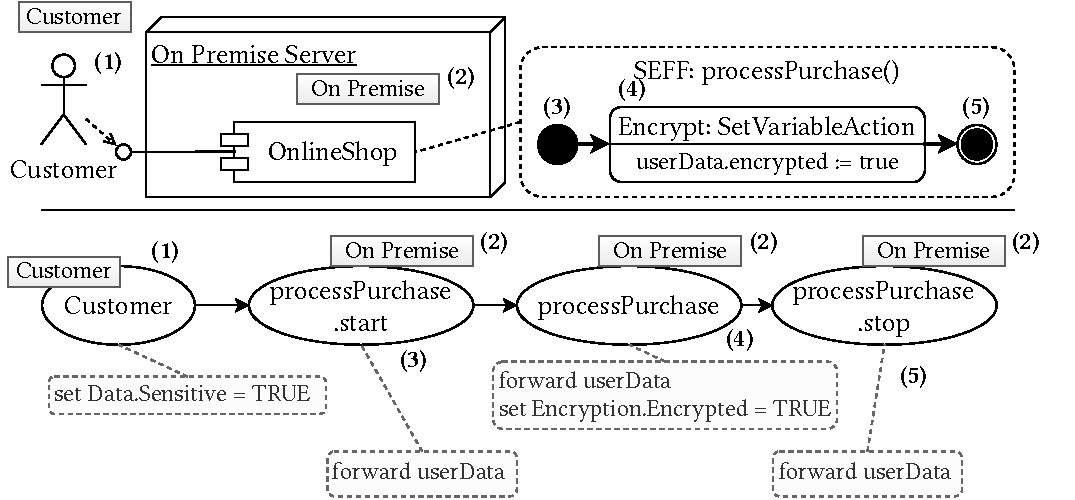
\includegraphics[width=\linewidth]{figures/chapter7/pcmextraction.pdf}
    \caption{Simplified \acf*{PCM} instance and the corresponding \acf*{TFG} with annotated node labels, data labels, and numbered transformation traces.}
    \label{fig:confidentialityanalysis:pcmextraction}
\end{figure}

\autoref{fig:confidentialityanalysis:pcmextraction} shows a simplified \ac{PCM} model based on the running example.
The model is annotated with confidentiality-related labels that represent characteristics of data storage like \emph{On Premise} and data processing like the encryption of \emph{userData} in the \emph{SetVariableAction}.
In the lower half, we show the extracted \ac{TFG}.
We annotate numbers to represent the transformation traces from the \ac{PCM} to the \ac{TFG}.
For every node, we perform a lookup of node labels, which can be annotated, e.g., to \emph{ResourceContainers}, or \emph{UsageScenarios}.
An exemplary lookup in the PCM model goes from the \emph{processPurchase} vertex to the \emph{Online Shop} component via the deployment to the \emph{On Premise Server} resource which is annotated with \emph{On Premise}.
Additionally, we convert the modeled system behavior to assignments representing the node's behavior, e.g., the encryption of \emph{userData}.
The default is the forwarding of labels, which represents the flow of data without further effects.
The transformation considers all information that is relevant for confidentiality analysis, e.g., data processing.
Other information is not transformed, e.g., components and servers do not cause additional elements in the \ac{TFG}.
This enables a system view from the perspective of the data.
We store all traces to the originating \ac{PCM} elements during the transformation.
This enables the evaluation of more advanced constraints in the data flow analysis.

In sum, \ac{TFG} represent a simple yet powerful way to reason about data flows, that can be extracted from \ac{PCM} models.
By adding node and data labels, they can represent the characteristics of the software system relevant for confidentiality analysis.
Data flow constraints can compare these labels to identify confidentiality violations.


\subsection{Label Propagation to Enable Scalable Confidentiality Analysis}

Annotated \acp{TFG} help to reason about data flows in software systems.
However, \acp{DFD} of realistic software systems contain several hundreds of nodes \cite{hahner_architecture-based_2023}.
\emph{Label propagation} has been proposed to automate the analysis, as manual analysis is not feasible \cite{seifermann_data-driven_2019}.
Put simply, label propagation propagates all data labels through all nodes of all \acp{TFG} with respect to the behavior of the nodes.

\begin{algorithm}
    \caption{Algorithm for vertex evaluation in \acfp*{TFG}}
    \label{alg:confidentialityanalysis:vertexevaluation}
    \begin{algorithmic}[1]
        \Procedure{\function{evaluateVertex}}{$\var{vertex}, \var{graph}$}
            \algindentskip
            \State $\var{vertex.nodelabels} \gets \function{evaluateNodeLabels}(\var{vertex})$ \Comment{Collect node labels} \label{alg:confidentialityanalysis:vertexevaluation:2}
            \State $\var{predecessors} \gets \function{getPredecessors}(\var{vertex})$
            \State $\var{vertex.datalabels} \gets \emptyset$
            \algblockskip

            \For{$\var{predecessor} \in \var{predecessors}$} \Comment{Collect data labels using recursion}
                \State $\var{vertex.datalabels} \gets \var{vertex.datalabels} \cup \function{evaluateVertex}(\var{predecessor}, \var{graph})$\label{alg:confidentialityanalysis:vertexevaluation:6}
            \EndFor
            \algblockskip

            \State $\var{result} \gets \function{evaluateNodeBehavior}(\var{vertex}, \var{vertex.datalabels})$ \label{alg:confidentialityanalysis:vertexevaluation:8}
            \State \Return{$\var{result}$}
            \algindentskip
        \EndProcedure   
    \end{algorithmic}
\end{algorithm}

\begin{algorithm}
    \caption{Algorithm for label propagation in \acfp*{TFG}}
    \label{alg:confidentialityanalysis:labelpropagation}
    \begin{algorithmic}[1]
        \Procedure{\function{labelPropagation}}{$\var{tfgs}$}
            \algindentskip

            \For{$\var{tfg} \in \var{tfgs}$} \Comment{Iterate over all independent TFGs}
                \State $\var{sink} \gets \function{getSink}(\var{tfg})$ \Comment{Start the evaluation at each sink}
                \State $\function{evaluateVertex}(\var{sink}, \var{tfg})$
            \EndFor
            \algblockskip

            \State \Return{$\var{tfgs}$}
            \algindentskip
        \EndProcedure   
    \end{algorithmic}
\end{algorithm}

\autoref{alg:confidentialityanalysis:vertexevaluation} shows the recursive algorithm of the vertex evaluation in label propagation, which resembles \ac{DFS}.
For each vertex, we first retrieve the vertex node labels in \autoref{alg:confidentialityanalysis:vertexevaluation:2}.
To simplify the algorithm, we denote the side effect of storing the labels in the vertex fields.
Afterward, we calculate the data labels that represent the output of the vertex and also store them in the corresponding vertex. 
This is achieved by recursively calling the calculation logic of all previous vertices and using the hereby calculated output labels as input, as shown in \autoref{alg:confidentialityanalysis:vertexevaluation:6}.
Before returning, we apply the behavior of the evaluated vertex to the input data labels in \autoref{alg:confidentialityanalysis:vertexevaluation:8}, e.g., altering the encryption label.
Note that we do not consider cycles in the propagation logic because \acp{TFG} represent \acp{DAG}.
Based on the evaluation of vertices, \autoref{alg:confidentialityanalysis:labelpropagation} shows the label propagation.
Here, we handle each \ac{TFG} separately as every \ac{TFG} represents independent data flows, and use the \emph{evaluateVertex} algorithm for the single sink of each \ac{TFG}.

\begin{figure}
    \centering
    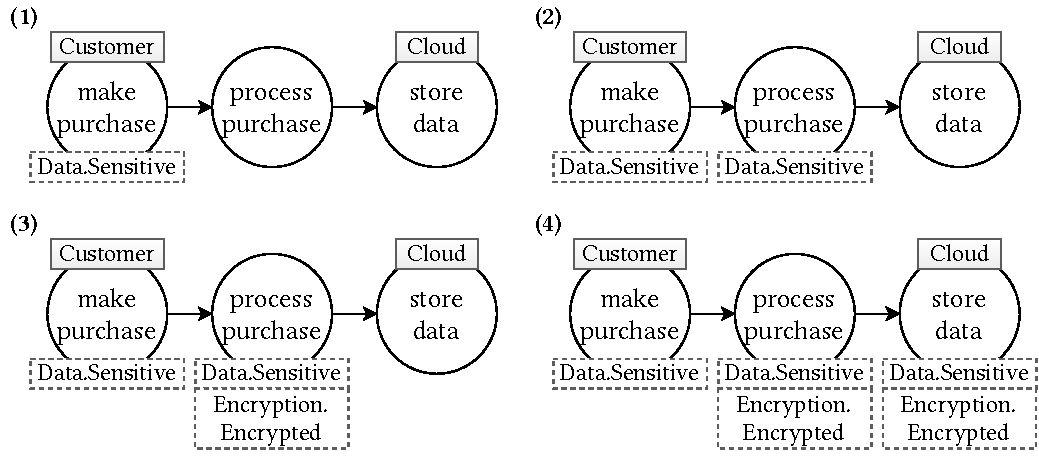
\includegraphics[width=\linewidth]{figures/chapter7/labelpropagation.pdf}
    \caption{Initial state, and intermediate and final results of the label propagation in a simple \acf*{TFG}. Node labels are highlighted gray, data labels have a dashed border.}
    \label{fig:confidentialityanalysis:labelpropagation}
\end{figure}

\autoref{fig:confidentialityanalysis:labelpropagation} shows four states of the label propagation in the simple \ac{TFG} introduced with \autoref{fig:confidentialityanalysis:annotatedtfg}.
First, we only display all node labels as these are not subject to label propagation but fixed, and also the label added in the \emph{make purchase} vertex.
This label is propagated to the \emph{process purchase} vertex in the second step.
By evaluating the behavior of this vertex, the label \emph{Encryption.Encrypted} is added in the third step.
In the fourth step, both labels are forwarded to the \emph{store data} vertex and the label propagation terminates.
After the label propagation, data flow constraints can compare node and data labels on each vertex without having to iterate over other vertices.
The resulting confidentiality analysis is scalable and has been evaluated on large \acp{DFD} with thousands of vertices \cite{schwickerath_tool-supported_2023}. 

\finding{Label propagation in \acfp{TFG} represents a simple and scalable way to automate data flow analysis regarding confidentiality.}





\section{Representing Uncertainty in Data Flow Analysis}%
\label{sec:confidentialityanalysis:representing}

The data flow analysis framework \cite{boltz_extensible_2024} presented in the previous section provides us with means for scalable confidentiality analysis and also with the notion of \acp{TFG} to reason about data flows.
The following discussion is based on this notion, and the differentiation between black-box and white-box analysis \cite{taghavi_survey_2023,heinrich_composing_2021}, presented in \autoref{sec:confidentialityanalysis:framework}.
We show different approaches to represent uncertainty in data flow analysis \cite{hahner_model-based_2023}.
These approaches differ in the use of data structures to analyze uncertainty and also in the use of information available for the analysis.
This addresses Problem \PR{3}{1}.

We addressed the representation of uncertainty in \ac{DFD}, in \autoref{sec:classification:dfd}, and in architectural models, in \autoref{sec:impactanalysis:representing}.
The former presented the distinction between \emph{primary} and \emph{secondary} uncertainty in \acp{DAG}, the latter related the five uncertainty types to elements of the unified modeling primitives \cite{seifermann_unified_2021} and to the \ac{PCM}.
We build on this to explain the representation of uncertainty in architecture-based data flow analysis.
As discussed previously, there are multiple approaches to data flow analysis under uncertainty which show different levels of uncertainty-awareness.
In the following, we discuss which information can be used for such analyses and present five levels of data flow analysis under uncertainty.


\subsection{Available Information in Uncertainty-Aware Data Flow Analysis}

\begin{table}
    \begin{tabularx}{\linewidth}{lX}
        \toprule
        Domain \, & Information categories \\
        \midrule
        Confidentiality & \mtl{
        \textbf{1.} Confidentiality violation occurrence, 
        \textbf{2.} Violated confidentiality\\requirements, 
        \textbf{3.} Location within the model,
        \textbf{4.} Analyzed data flows,\\ 
        \textbf{5.} State of data at the violation}
        \\
        \midrule
        Uncertainty & \mtl{
        \textbf{6.} Uncertainty source,
        \textbf{7.} Uncertainty properties and classification,\\
        \textbf{8.} Uncertainty impact within the model,
        \textbf{9.} Uncertainty interactions,\\
        \textbf{10.} Uncertainty mitigation}\\
        \bottomrule
    \end{tabularx}
    \caption{Available information categories for uncertainty-aware confidentiality analysis.}%
    \label{table:confidentialityanalysis:informationcategories}
\end{table}

\autoref{table:confidentialityanalysis:informationcategories} shows information categories regarding confidentiality and uncertainty.
The confidentiality information categories are derived from data flow-based analyses of architectural models \cite{seifermann_unified_2021}.
The categories include knowledge about the existence of confidentiality violations (\textbf{1.}) and the related violated requirements (\textbf{2.}).
We consider this to be the result of any usable analysis.
In the running example, the confidentiality requirements of storing personal data could be violated.
Additionally, such analyses can point to the location within the architectural model (\textbf{3.}) and the critical data flow (\textbf{4.}) where the violation occurred.
In the running example, the violating data flow could be from the \emph{Customer} to the \emph{Database Service}, where the violation happens.
Last, the state of the data causing the violation can be considered (\textbf{5.}).
This can be realized using labels like personal data, or deployment in the cloud.
The data flow analysis framework presented in \autoref{sec:confidentialityanalysis:framework} uses all five categories in the analysis and also when presenting identified confidentiality violations.
Nevertheless, analyses with a simplified interface are imaginable, e.g., black-box analyses only report the existence of violations.

The uncertainty information categories are derived from the uncertainty management in \acfp{SAS} \cite{hezavehi_uncertainty_2021} and \acfp{CPS} \cite{acosta_uncertainty_2022} and also based on the handling of uncertainty regarding confidentiality \cite{hahner_classification_2023}.
By investigating an uncertainty source (\textbf{6.}) in the model or its environment \cite{acosta_uncertainty_2022}, it can be described more precisely, e.g., based on a classification (\textbf{7.}), as discussed in \autoref{ch:classification}.
Also, the uncertainty's impact (\textbf{8.}) on the software architecture can be derived and expressed.
We discussed the distinction between uncertainty sources and their impact in \autoref{sec:classification:relation}.
In a software system with multiple uncertainty sources, potential uncertainty interactions are also important to consider (\textbf{9.}).
This is related to the \acf{UIP} and has been discussed with regard to \acp{DFD} in \autoref{sec:classification:dfd}.
Last, by analyzing the architectural model, mitigation techniques (\textbf{10.}) can be chosen already at design time \cite{hezavehi_uncertainty_2021}.
In our running example, we identified four uncertainty sources (\U{1} -- \U{4}), which were also classified.
We analyzed the potential impact of these uncertainties using uncertainty impact analysis in \autoref{ch:impactanalysis}.
For instance, uncertainty \U{4} causes a broad impact in the \emph{Database Service}.
We also have means to represent simple uncertainty interactions, e.g., between secondary and primary uncertainty sources in \acp{DAG}, see \autoref{sec:classification:dfd}.
For example, we identified an uncertainty interaction between the deployment in Uncertainty \U{3} and the provider trustworthiness in Uncertainty \U{4}.
Last, design time approaches can also support the tool-supported mitigation uncertainty that causes confidentiality violations.
We consider this to be out of scope for this work as we focus on the uncertainty-aware analysis as a required prerequisite for mitigation \cite{weyns_introduction_2020}.


\subsection{Levels of Uncertainty-Awareness in Data Flow Analysis}

Based on these information categories (\textbf{1.} -- \textbf{10.}), we define five levels (\level{0} -- \level{4}) of data flow analyses under uncertainty.
Regarding model-based confidentiality analysis, showing violations (\textbf{1.}) with the related reason (\textbf{2.}) to software architects is considered to be the minimum viable information \cite{hahner_modeling_2021}.
The analysis results become more expressive by also showing the location (\textbf{3.}), analyzed data flows (\textbf{4.}) and the state of the data (\textbf{5.}).


\paragraph{L0: No uncertainty-awareness}\label{awarenesslevel:0}
Data flow analyses that provide neither modeling nor analysis support for uncertainty show \emph{no uncertainty-awareness}.
This affects the precision and comprehensiveness \cite{hahner_architectural_2021} of confidentiality violations as the models and the analysis fall short of representing the real world, as discussed in the introduction of this chapter.
The lack of awareness becomes visible in over-estimations and also in missing violations \cite{seifermann_architectural_2022}.
In our running example, a confidentiality analysis that ignores uncertainty would miss all violations due to the identified uncertainty sources.
This level represents the state of the art before our endeavors \cite{seifermann_architectural_2022,hahner_dealing_2021,seifermann_detecting_2022}.
Note that this does not mean that such analyses cannot be extended to consider uncertainty \cite{hahner_dealing_2021}.


\paragraph{L1: Naive approach to uncertainty-awareness}\label{awarenesslevel:1}
The \emph{naive approach} to handling uncertainty is to directly model its impacts (\textbf{8.}).
This means manually altering models to respect the change caused by uncertainty.
In our running example, we can model different variants, e.g., with the deployment on-premise or in the cloud.
The analysis rejects the software architecture if there exist confidentiality violations in at least one variant.
By directly representing the uncertain effect within the model, we lose all information about the source (\textbf{6.} and \textbf{7.}).
Especially when considering multiple uncertainty impacts, all variant combinations and interactions (\textbf{9.}) have to be manually modeled, which requires extensive manual effort. 
Additionally, changes to the model have to be done in all variants.
While this yields more comprehensive results, it still highly lacks precision \cite{bitschi_uncertainty-aware_2022} and requires an unreasonably high manual effort.


\paragraph{L2: Scenario-awareness}\label{awarenesslevel:2}
\emph{Scenario-aware} analyses build on the idea of representing uncertainty sources (\textbf{6.}) as model variations separate from the modeled software architecture.
Here, variability models, model variations, or partial models represent common ways of expressing the potential outcomes of uncertainty \cite{troya_uncertainty_2021}.
We also included this level of information in our classification (\textbf{7.}).
The option \emph{Scenario Uncertainty} in the category \emph{Type} expresses a state of knowledge where the effects of an uncertainty source can be described using scenarios.
As classified in \autoref{sec:classification:runningexample}, all uncertainty sources are describable using scenarios in our running example.
The main difference to the \emph{naive approach} (\level{1}) is the automated application of these variations to the architectural model.
This approach greatly reduces the manual modeling effort, as software architects only have to specify the point of variation and do not realize the variation and thus the impact of the uncertainty (\textbf{8.}) itself.
The analysis rejects only such architecture variants that violate confidentiality, without considering the location (\textbf{3.}), data flows (\textbf{4.}) or the state of the data (\textbf{5.}).
Realized as a black-box analysis extension, this lacks precision because it only considers the existence of violations (\textbf{1.}) of requirements (\textbf{2.}) in selected scenarios.
Last, while the manual effort is reduced, the complexity of calculating variations of variations can quickly lead to a combinatorial explosion, as discussed in the context of design space exploration \cite{koziolek_automated_2011}.


\paragraph{L3: Graph-awareness}\label{awarenesslevel:3}
To overcome the limitations regarding scalability and expressiveness of the results, \emph{graph-aware} analyses can be used.
Realized as white-box extension \cite{boltz_architectural_2021,bitschi_uncertainty-aware_2022,boltz_handling_2022,hahner_architecture-based_2023} of a data flow analysis, this enables the connection of uncertainty sources (\textbf{6.}) to analyzed data flows (\textbf{4.}).
This is the first level that is able to represent uncertainty as a first-class concern, both within the architectural model and \acp{DFD}.
It builds on the idea of representing uncertainty as a set of scenarios, introduced with the \emph{scenario-aware} approach (\level{2}).
However, by relating the variation directly to the analyzed data flows, a higher expressiveness can be reached.
\emph{Graph-aware} analyses thus cover all five confidentiality related categories (\textbf{1.} -- \textbf{5.}) and are able to represent Uncertainty sources (\textbf{6.}), their properties (\textbf{7.}), and their impact (\textbf{8.}) directly within the model.
Additionally, they can achieve higher scalability as uncertainty sources in different data flows can be analyzed independently, which partially addresses the combinatorial explosion.
Put simply, in a real-world software system with many independent data flows, the effects of uncertainties can be separate.
To leverage this, the analysis requires awareness about the analyzed graph, which represents the main difference to the \emph{scenario-aware} approach (\level{2}).
In our running example, the \emph{scenario-aware} approach can only try out all variations, while the \emph{graph-aware} approach can use the information of the different data flows from the \emph{Customer}.
However, this does not lead to more accurate results---both approaches differ in expressiveness and scalability.
Note that we renamed \enquote{data flow-awareness} to \enquote{graph-awareness} compared to the original publication \cite{hahner_model-based_2023} to increase clarity\footnote{Like an uncertainty-aware uncertainty analysis, a data flow-aware data flow analysis does not make too much sense. However, I am not so sure about the former---what about antifragility?}.


\paragraph{L4: Impact-awareness}\label{awarenesslevel:4}
The \emph{graph-aware} analysis (\level{3}) is able to consider the effect of single uncertainty sources, both within the architectural model and \acp{DFD}.
However, the impact of uncertainties can also affect other uncertainties, i.e., uncertainty interaction.
This becomes visible in uncertainty-aware data flow analysis when an uncertainty alters a data flow that contains another uncertainty.
In our running example, such an interaction happens with Uncertainty \U{3} about the deployment and Uncertainty \U{4} about the provider's trustworthiness.
The former can impact the data flow so that it does not flow to a location that is affected by the latter, as shown in \autoref{fig:classification:dag}.
By understanding such interactions and the transitive effects of propagating uncertainty, and by incrementally analyzing data flows, \emph{impact-awareness} can be reached.
This level builds on the findings of \emph{scenario-aware} (\level{2}) and \emph{graph-aware} (\level{3}) approaches and thus yields analysis results with the same accuracy regarding confidentiality violations.
However, by also considering uncertainty interactions (\textbf{9.}), a higher expressiveness and scalability can be reached.


These five levels (\level{0} -- \level{4}) of uncertainty-aware data flow analysis provide the terminology to present the different research approaches hereafter.
Although the terminology is related to orders of ignorance \cite{armour_five_2000} or the levels of uncertainty \cite{bures_capturing_2020}, there exists no direct mapping, as we only focus on already identified uncertainty sources, see \autoref{ch:classification}.
Note that these levels do not represent a comprehensive list but only a classification for the scope of this work.
Further classes are imaginable, e.g., regarding the mitigation (\textbf{10.}), or by using advanced algorithms for analyzing uncertainty impacts and confidentiality violations.

Other classifications of uncertainty-aware data flow analyses are useful in addition to these levels.
Regarding the wide variety of uncertainty sources, some analyses might not cover all types of uncertainty \cite{troya_uncertainty_2021,PSUM}.
\textcite{troya_uncertainty_2021} conduced a \acf{SLR} with 123 papers and found that the majority of approaches only consider less than three types of uncertainty, e.g., behavior uncertainty combined with design uncertainty or belief uncertainty combined with measurement uncertainty.
Here, we build on the five uncertainty types of the category \emph{Architectural Element Type} of our classification, introduced in \autoref{sec:classification:classification}.
We call an uncertainty-aware data flow analysis to be \emph{type-specific} if it supports a subset of these uncertainty types.
Uncertainty \emph{type-agnostic} approaches support all five uncertainty types.

\finding{Uncertainty-aware data flow analysis approaches can be classified depending on the supported uncertainty types and the utilization of available information within the analysis.
This enables the classification of approaches that differ in accuracy, expressiveness, and scalability.}


\subsection{Examples for Uncertainty-Aware Data Flow Analysis}

\begin{table}
    \begin{tabularx}{\linewidth}{llX}
        \toprule
        \multicolumn{2}{l}{Uncertainty source} & Uncertainty scenarios \\
        \midrule
        \U{1} & User input & Valid input \,/\, Erroneous input \,/\, Malicious input \\
        \U{2} & Data processing & None \,/\, Encryption \,/\, Validation \,/\, Both \\
        \U{3} & Component deployment & On premise \,/\, Cloud service \\
        \U{4} & Provider trustworthiness & Trustworthy \,/\, Suspicious \\
        \bottomrule
    \end{tabularx}
    \caption{Uncertainty scenarios of all uncertainty sources of the running example.}%
    \label{table:confidentialityanalysis:scenarios}
\end{table}

We illustrate the different levels (\level{0} -- \level{4}) and types of uncertainty-aware analysis using our running example.
As discussed previously, all four uncertainty sources (\U{1} -- \U{4}) represent \emph{Scenario} uncertainty.
Based on the findings of \textcite{troya_uncertainty_2021}, we can thus describe the variation scenarios of all four uncertainty sources.
\autoref{table:confidentialityanalysis:scenarios} shows the possible scenarios for each uncertainty source that has been introduced in \autoref{ch:runningexample}.

A data flow analysis that lacks uncertainty-awareness (\level{0}) is not able to consider these uncertainty sources.
Speaking in terms of variations, these analyses select one scenario of each uncertainty, i.e., the architectural model without modification.
Only if this default scenario violates confidentiality, the violation is identified.
The \emph{naive} approach (\level{1}) to uncertainty-aware analysis is to manually model all combinations of all scenarios.
As this approach must assume the dependence of all uncertainty sources and their scenarios, we use the Cartesian product \cite{de_finetti_theory_2017}.
Thus, software architects have to manually model $3 \cdot 4 \cdot 2 \cdot 2 = 48$ software architectures in the running example, which is not feasible.

Using variation models in \emph{scenario-aware} analysis (\level{2}), software architects only model the variation points, i.e., all $3 + 4 + 2 + 2 = 11$ scenarios of the running example.
The variation creation can be automatized \cite{walter_architecture-based_2023}, which reduces the manual modeling effort, i.e., $11 < 48$.
However, the assumption on the dependence of all uncertainty sources remains and thus, all resulting $48$ variants have to be analyzed.
With larger amounts of uncertainty sources or scenarios, this can quickly lead to the already discussed combinatorial explosion \cite{koziolek_automated_2011}.

The \emph{graph-aware} approach (\level{3}) addresses this issue.
As discussed with uncertainty propagation in \ac{DFD} in \autoref{sec:impactanalysis:dfdpropagation}, uncertainty sources can be considered independently in all independent data flows.
This reduces the number of variants that have to be analyzed in all non-trivial software systems, i.e., in software systems with more than a single data flow.
Our running example comprises three independent data flows: Retrieving the support contact, querying items, and making purchases, see \autoref{fig:runningexample:dfd}.
Using the \ac{DFD} as a data structure for the analysis, the \emph{graph-aware} approach yields more comprehensive results.
In our running example, we can see that the data flow representing the support contact retrieval is neither affected by uncertainty nor violates confidentiality.

Last, the \emph{impact-aware} approach (\level{4}) builds on this and also considers uncertainty interactions.
We discussed this with the interaction of the uncertainties \U{3} and \U{4} in \autoref{sec:classification:dfd}.
Note that we do not classify the uncertainty impact analysis presented in \autoref{ch:impactanalysis} as it does not represent a confidentiality analysis.
However, this analysis could be considered as type-agnostic and graph-aware, as all five uncertainty types can be propagated on the \ac{DFD}.
This analysis does not reach \emph{impact-awareness} because the effect of changes to the software architecture is ignored and overestimated.

\begin{table}
    \begin{tabularx}{\linewidth}{llXX}
        \toprule
        \multicolumn{2}{l}{Level of awareness} & Uncertainty type-specific & Uncertainty type-agnostic \\
        \midrule
        \level{0} & None & \multicolumn{2}{l}{Uncertainty-unaware data flow analysis \cite{seifermann_detecting_2022,seifermann_architectural_2022,boltz_extensible_2024}} \\
        \midrule
        \level{1} & Naive & - & - \\
        \level{2} & Scenario-aware & Approach for structural uncertainty, \autoref{sec:confidentialityanalysis:structural} & - \\
        \level{3} & Graph-aware & Approach for environmental uncertainty, \autoref{sec:confidentialityanalysis:environmental} & Approach for tracing uncertainty, \autoref{sec:confidentialityanalysis:tracing} \\
        \level{4} & Impact-aware & - & Approach for impact-aware analysis, \autoref{sec:confidentialityanalysis:abunai} \\
        \bottomrule
    \end{tabularx}
    \caption{Awareness levels and type specificity of uncertainty-aware data flow analysis approaches.}%
    \label{table:confidentialityanalysis:awareness}
\end{table}

In the remainder of this chapter, we present four approaches to uncertainty-aware data flow analysis.
\autoref{table:confidentialityanalysis:awareness} classifies these approaches according to the five levels (\level{0} -- \level{4}) and with regard to the type specificity.
We also add the \emph{uncertainty-unaware} approach of architecture-based data flow analysis for reference purposes.

The data flow analysis framework \cite{boltz_extensible_2024} without explicit support for modeling or analyzing uncertainty as presented in \autoref{sec:confidentialityanalysis:framework} represents Level \level{0}.
We do not distinguish between the type specificity as the analysis does support no uncertainty at all.
We also do not present naive approaches (\level{1}) in this thesis, as they do not represent a noteworthy improvement on the state of the art.
The first approach discussed in this thesis is the \emph{scenario-aware} analysis (\level{2}) of structural uncertainty, e.g., regarding uncertain component deployment.
Due to the previously discussed limitations of scenario awareness, we continue with an approach for environmental uncertainty that is \emph{graph-aware} (\level{3}).
Afterward, we present the first uncertainty type-agnostic approach for data flow analysis.
This approach covers all five uncertainty types and traces confidentiality violations to variations caused by uncertainty sources.
Last, we further enhance this concept and present an uncertainty \emph{impact-aware} approach (\level{4}) for data flow analysis regarding confidentiality.
Generally speaking, a higher level and being type-agnostic is superior.





\section{Uncertainty Type-Specific Data Flow Analysis}%
\label{sec:confidentialityanalysis:typespecifc}

In this section, we present the first two approaches for uncertainty-aware data flow analysis.
The first approach is \emph{scenario-aware} (\level{2}) and considers structural uncertainty within the software architecture.
The second approach is \emph{graph-aware} (\level{3}) and deals with environmental uncertainty concerning user privileges in access control.
Both approaches are \emph{type-specific} as they are tailored to one uncertainty type.
This addresses Problem \PR{3}{2}.


\subsection{Data Flow Analysis Under Structural Uncertainty}%
\label{sec:confidentialityanalysis:structural}

As the name suggests, structural uncertainty affects the structure of the software architecture.
Examples are \acfp{ADD} regarding components or their deployment.
As this represents uncertainty in the software design \cite{mcconnell_software_1998}, it is best represented using variation points \cite{troya_uncertainty_2021}.
Regarding the variation creation, there already exist approaches such as design space exploration \cite{sobhy_evaluation_2021}.
For this analysis approach, we use the architectural optimization approach PerOpteryx \cite{koziolek_automated_2011,koziolek_performance_2010,koziolek_peropteryx_2011,martens_automatically_2010} and combine it with data flow analysis \cite{seifermann_detecting_2022}.
Software architects first model different design decisions. 
These design decisions are then used to automatically create different architecture variations, which are analyzed for confidentiality.
Since we reuse PerOpteryx for the design space exploration, this approach can consider additional quality attributes, such as performance, or costs, and calculate the Pareto optimal candidate.
This optimization enables software architects to make informed trade-off decisions between quality metrics.

PerOpteryx \cite{koziolek_peropteryx_2011,koziolek_automated_2011} is a design space exploration and optimization approach for the \ac{PCM}. 
It uses evolutionary search algorithms and calculates the Pareto optimal architectural variation. 
The different variation points of the architecture are specified in the design decision model. 
Here, software architects can define which entities in the software architecture can be configured. 
For instance, in our running example, a design decision is the deployment of the \emph{Database Service} component to the \emph{On Premise Server} or to the \emph{Cloud Service}.
Due to the relation of \acp{ADD} and uncertainty, explained in \autoref{sec:classification:relation}, we can use this model to express structural uncertainty sources and their scenarios.
The different quality attributes are defined as quality dimensions.
Each generated architectural variation that is evaluated for quality attributes is called a candidate. 
Besides the optimal candidates, PerOpteryx also yields all the investigated candidates.
There exist various quality dimensions, such as costs or performance. 
However, there is no quality dimension for confidentiality, which is required for the connection to the data flow analysis. 
While PerOpteryx already contains a security dimension \cite{busch_modelling_2016}, we decide against it since we want to explicitly target confidentiality. 
The existing security dimension is focused more on the costs of introducing security measures and the costs of failure.

\begin{figure}
    \centering
    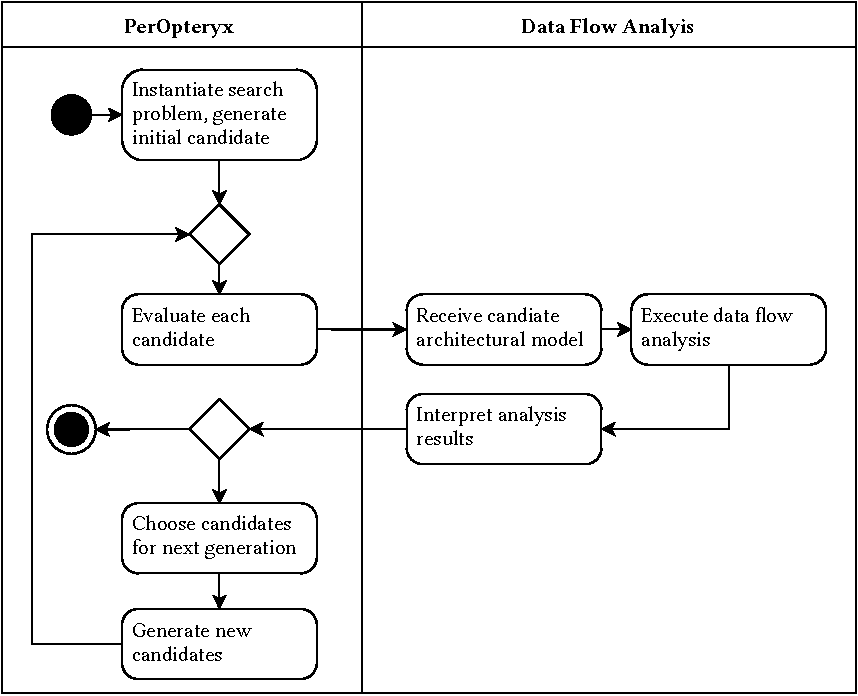
\includegraphics[width=\textwidth]{figures/chapter7/peropteryx.pdf}
    \caption{Activity diagram showing the interplay of PerOpteryx and the data flow analysis using swimlanes.}
    \label{fig:confidentialityanalysis:peropteryx}
\end{figure}

We add a new confidentiality violation to PerOpteryx that is modeled as real values where decreasing values are better solutions \cite{liu_design_2021}.
We map these to a binary classification for the confidentiality analysis results.
For each quality dimension, PerOpteryx defines handlers, which can analyze a model for the given quality dimension. 
Therefore, we define a new confidentiality handler for the confidentiality domain, which acts as an adapter between PerOpteryx and the data flow analysis.
This handler forwards the current architecture candidate models to the data flow analysis and interprets the analysis result.
The interpretation of confidentiality violations is binary with the classes \emph{confidentiality ensured} and \emph{confidentiality violated}. 
Our adapter transforms \emph{confidentiality ensured} to -1 and \emph{confidentiality violated} to 1.
This binary interpretation is required as there is currently no meaningful way of further quantifying the results of the data flow analysis \cite{walter_architectural_2022}.
The results enable the PerOpteryx optimization to rank confidential candidates higher than non-confidential ones.
After the execution of PerOpteryx, software architects get a result with all tested variations and the Pareto optimal version.
\autoref{fig:confidentialityanalysis:peropteryx} shows this procedure of PerOpteryx \cite{koziolek_peropteryx_2011} using the data flow analysis.
For the sake of simplicity, we only depict a single quality dimension, i.e., confidentiality.
Other quality dimensions can be represented by additional swimlanes that are called during the candidate evaluation.

In our running example, only Uncertainty \U{3} about the deployment represents structural uncertainty.
This uncertainty can be modeled as \ac{ADD} in the design decision model.
PerOpteryx then creates all variations, i.e., the deployment on the \emph{On Premise Server} and on the \emph{Cloud Service}.
Both candidates are forwarded to the data flow analysis.
The former ensures confidentiality while the latter causes a confidentiality violation and thus returns the value 1.
Last, the deployment \emph{on premise} is returned as the optimal version.

There are three disadvantages and two advantages of this approach.
First, being type-specific to structural uncertainty limits the applicability to other uncertainty types that can affect confidentiality.
Second, the black-box coupling of PerOpteryx with the data flow analysis only shows the existence of violations but no further information, e.g., on the location, or affected data flows, which impedes the interpretation by software architects.
Third, confidentiality violations have no continuous occurrence, i.e., small changes to the software architecture can have a large impact.
This is a known limitation of PerOpteryx and is described as a rugged search landscape with non-continuous jumps \cite{koziolek_automated_2011}.
In the worst case, this can cause PerOpteryx to test out all possible variations, i.e., the Cartesian product, which resembles a brute-force approach.
Nevertheless, this coupling is superior to the \emph{naive} approach (\level{1}) as it notably reduces the modeling effort.
Additionally, combining confidentiality analysis with the optimization of other quality attributes represents a more realistic application scenario, where informed trade-off decisions are made by software architects.
No other approach presented in this thesis provides such functionality without requiring the combination with other architecture evaluation approaches \cite{sobhy_evaluation_2021}.

\finding{On the one hand, the black-box coupling of data flow analysis with architectural optimization is complicated by the non-continuous occurrence of confidentiality violations, which increases the complexity of the optimization problem.
On the other hand, extending an existing software architecture optimization approach simplifies the joint evaluation of multiple quality attributes.}

\begin{algorithm}
    \caption{Algorithm for scenario-aware data flow analysis under uncertainty}
    \label{alg:confidentialityanalysis:scenarioaware}
    \begin{algorithmic}[1]
        \Procedure{\function{analyzeScenarioAware}}{$\var{model}, \var{constraint}, \var{uncertainties}$}
            \algindentskip
            \State $\var{violations} \gets \emptyset$
            \State $\var{variations} \gets \function{generateAllVariations}(\var{model}, \var{uncertainties})$
            \algblockskip

            \For{$\var{variation} \in \var{variations}$} \Comment{Analyze all possible variations}
                \State $\var{violations} \gets \var{violations} \cup \function{analyze}(\var{variation}, \var{constraint})$ 
            \EndFor
            \algblockskip

            \State \Return{$\var{violations}$}
            \algindentskip
        \EndProcedure   
    \end{algorithmic}
\end{algorithm}

To conclude, we present a more general approach to \emph{scenario-aware} data flow analysis under uncertainty.
Put simply, \emph{scenario-awareness} (\level{2}) is generating all possible variations of the architectural model and then analyzing them to identify confidentiality violations \cite{walter_architecture-based_2023}.
This is shown in \autoref{alg:confidentialityanalysis:scenarioaware}.
However, such analyses are prone to the combinatorial explosion of uncertainty sources and their scenarios.
Additionally, the analysis results are hard to interpret without further processing.
For instance, in our running example, software architects would have to interpret the confidentiality violations of 48 architectural models to asses four uncertainty sources.
We posit that \emph{scenario-aware} analysis should only be used in specific cases, e.g., combined with design space exploration. 


\subsection{Data Flow Analysis Under Environmental Uncertainty}%
\label{sec:confidentialityanalysis:environmental}

Environmental uncertainty arises from the system context, e.g., in the system usage, or its resource environment.
Here, sensors are especially often referred to as uncertainty source \cite{camara_addressing_2022,camara_uncertainty_2024,perez-palacin_uncertainties_2014,camara_software_2020,weyns_introduction_2020}.
Examples are sensor failure, sensor noise, or sensor inaccuracy \cite{hahner_arcn_2024}.
We discussed the relation of such uncertainty and confidentiality in \autoref{ch:classification}, where we classified such uncertainty as \emph{environment} or \emph{input} uncertainty.
A particular challenge is the relation of environmental uncertainty and access control \cite{bures_capturing_2020,heinrich_dynamic_2023}.
Broken access control can lead to severe confidentiality violations and is listed as the TOP 1 entry in the \ac{OWASP} Top 10 \cite{OWASPTop10}.
To address this, we present our second approach to uncertainty-aware data flow analysis: A \emph{graph-aware} analysis (\level{3}) of environmental uncertainty.
The following description is based on our publication about this approach \cite{boltz_handling_2022}.

A common measure to ensure confidentiality are access control mechanisms that authorize access or processing of data. 
Depending on the underlying access control model, various sources of information are used to determine whether access is granted. 
Services use different sources, e.g., sensors, to acquire information. 
Services process the information and provide a resulting access control attribute, e.g., a role or a location, that can be used by the access control system. 
However, these services introduce a degree of uncertainty to the access control system. 
This uncertainty results from influencing factors of the environment when acquiring the information. 
The influence of the factors on the access control system can result in reduced validity of statements about confidentiality. 
Depending on the system design, software architects or security experts might already be able to identify potential influencing factors. 
For example, the ability of a GPS service to provide an accurate position is highly dependent on its surroundings, like buildings. 

We extend our running example presented in \autoref{ch:runningexample} to illustrate this challenge.
We add an \emph{Admin} user who can directly access the \emph{Database Service} for maintenance \cite{walter_context-based_2023}.
To enhance security, access to the database is only permitted if the accessing actor is located inside of the office. 
The location of each actor is monitored using a GPS location service.
Here, we can choose a high-sensitivity GPS sensor, short \emph{HSGPS}, or the normal GPS sensor in the actor's mobile phone.
For this example, we focus on the differences between running the two types of GPS sensors indoors \cite{kjaergaard_indoor_2010}, where the sensor quality can degrade.
Once the actor enters the building, the signal attenuation increases which results in a reduced signal-to-noise ratio.
A reduced signal-to-noise ratio increases the time needed to acquire satellite data and calculate a position, and the amount of positioning errors \cite{kjaergaard_indoor_2010}. 
While the HSGPS sensors are powerful enough to provide accurate positioning, the accuracy of the embedded GPS sensor of the mobile phone suffers when used inside, which leads to uncertainty regarding the actual position. 
This reduced accuracy introduces uncertainty about the position \cite{camara_software_2020}. 
When this information is used within access control, it could lead to the wrong classification of the \emph{Admin} or other actors in the building.

To address such uncertainty, we present an approach for handling known, environmental uncertainty in access control during design time.
To this end, we enable the explicit representation of the known uncertainty and integrate the additional knowledge into an analysis. 
We propose a notion of \emph{confidence} in the validity of access control attributes, based on three types of influencing factors of the system environment.
We then show an access control analysis that integrates \emph{confidence} into our data flow analysis framework, presented in \autoref{sec:confidentialityanalysis:framework}. 
We propose the use of \acfp{FIS} \cite{klir_fuzzy_1995} to combine influencing factors to a resulting confidence value.

\begin{figure}
    \centering
    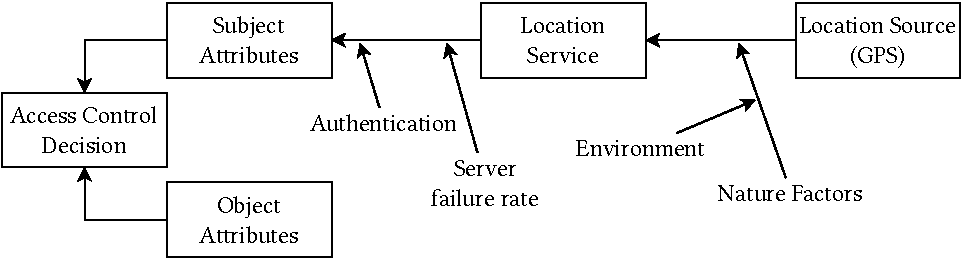
\includegraphics[width=\linewidth]{figures/chapter7/trustchain.pdf}
    \caption{A simplified trust chain that incorporates types of factors of the GPS location example.}
    \label{fig:confidentialityanalysis:trustchain}
\end{figure}

\textcite{hu_guide_2014} provide a definition and considerations regarding \acf{ABAC}. 
They describe a trust chain, concerning the attributes used to make access control decisions. 
Trust chains help determine the ownership of information and services, as well as requirements for technical solutions to establish valid trust relationships. 
The predicate of a trust relationship revolves around the idea that the access control system can trust the validity or correctness of the information, supplied by the owner, e.g., an authorization service. 
Depending on the access control model, many trust relationships are required to achieve a properly working access control system.
\autoref{fig:confidentialityanalysis:trustchain} shows a trust chain of a location attribute. 
The \emph{subject attributes} have a trust relationship with the \emph{location service}, which in turn has a trust relationship with the \emph{location source}. 
As indicated by the additional arrows, the trust relationships are impacted by influences of the environment of the system.

\textcite{ardagna_supporting_2006} define a confidence value that combines the service used for location determination and environmental conditions. Similar to the trust of \textcite{hu_guide_2014}, confidence describes the certainty that a location is valid, which is dependent on the environment.
Based on the work of \textcite{hengartner_distributed_2007} we can identify three environmental factors that influence the uncertainty in access control. 
These factors can be applied to access control attributes, align well with the idea of trust relationships of \textcite{hu_guide_2014} and can be represented in software architecture.
We describe the three factors in the following.

First, the \emph{source} that is used by the service to obtain information that is needed for the access control attribute. 
Location information, for example, might be derived from a physical access control mechanism or GPS data. 
Each of these sources has a different margin of error or accuracy.
Second, \emph{nature factors} that either influence the source's or the service's ability to return correct information or attributes.
Depending on the sensitivity and rating, the accuracy with which GPS sensors can determine a location is heavily influenced by the physical environment, e.g., surrounding buildings \cite{kjaergaard_indoor_2010}, and weather conditions, e.g. cloudy sky \cite{ardagna_supporting_2006}.
Third, the \emph{age} of an attribute, which, depending on the underlying information, might degrade validity. 
Depending on the attribute, age can be a combination of the time it took to gather the information from the source, the time it takes to process the information to an access control attribute and the overall time that has passed since this access control attribute has been created.

These factors and the associated uncertainties are all known, but especially when multiple factors need to be combined, their influence on the validity of an access control attribute is hard to describe. 
To provide a way of representing this known uncertainty, we define a notion of \emph{confidence} in the validity of access control attributes.
Confidence combines the known uncertainty of environmental factors into a single value, which represents the level of confidence that a corresponding attribute is valid. 
Confidence and the known uncertainty are not directly associated with an access control attribute, but rather with the service that is used by the system to derive the attribute. 
A service uses a source to receive information. 
The service processes this information into an attribute and provides it to the access control system.
The factors decrease the overall accuracy and thereby influence confidence. 
Any of the factors shown in \autoref{fig:confidentialityanalysis:trustchain} might reduce confidence in the location attribute.
For instance, this can result in \emph{high confidence} in access control attributes, that are derived by services that use the HSGPS sensors, and \emph{low confidence} in access control attributes derived by services using the mobile phone GPS sensor.

To combine these factors, we propose the use of fuzzy inference in the form of a \acp{FIS} \cite{klir_fuzzy_1995}.
For over two decades, fuzzy sets and fuzzy logic have been used to describe uncertainty \cite{klir_fuzzy_1995}. 
Fuzzy logic is also used in related work regarding design time uncertainty and uncertainty in access control \cite{cheng_fuzzy_2007,esfahani_guidearch_2013,hosmer_using_1992,troya_uncertainty_2021}.
A \ac{FIS} is made up of four main components \cite{klir_fuzzy_1995}:
A \emph{fuzzifier} first translates the crisp values of environmental factors into fuzzy values, by applying them to a set of membership functions. 
The \emph{fuzzy inference engine} uses the fuzzy input from the fuzzifier and rules to infer a fuzzy output. 
The \emph{defuzzifier} translates the fuzzy output of the inference engine to a confidence value, by aggregating the fuzzy outputs.
These steps are supported by a shared \emph{knowledge base}.

\begin{figure}
    \centering
    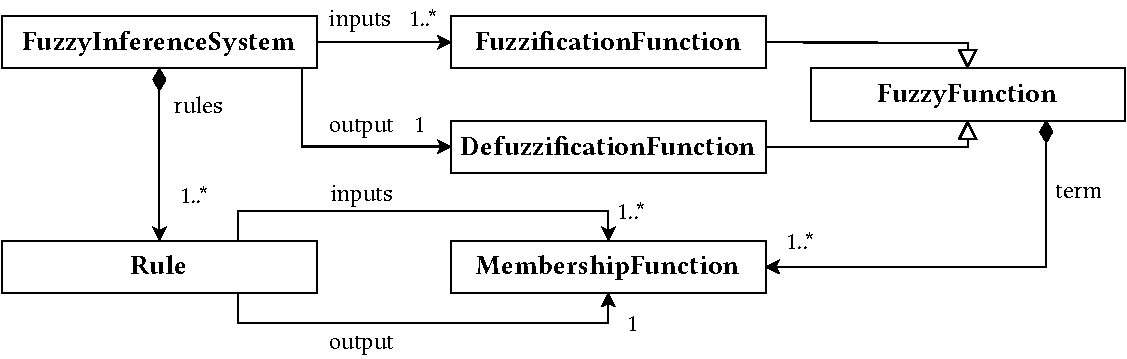
\includegraphics[width=\linewidth]{figures/chapter7/fis-metamodel.pdf}
    \caption{Excerpt from the class diagram of the \acf*{FIS} meta model.}
    \label{fig:confidentialityanalysis:fismetamodel}
\end{figure}

We present a \ac{FIS} metamodel as a way to enable software architects to create \acp{FIS}.
\autoref{fig:confidentialityanalysis:fismetamodel} shows an excerpt of the class diagram representation of the FIS metamodel. 
We represent the environmental factors as \emph{fuzzification functions}, which are made up of \emph{membership functions}. 
Each membership function defines a fuzzy set and represents a \emph{linguistic value} the environmental factor can take on. 
The corresponding membership functions define a degree of membership to the fuzzy set within an interval of $[0,1]$. 
Using the value of the environmental factor, e.g. a $30 \%$ signal-to-noise ratio, the fuzzifier calculates a degree of membership for each fuzzy set of the associated fuzzification function. 
In our running example, the signal-to-noise ratio can take on the linguistic values of \emph{low} and \emph{high}. 
The linguistic values of age are \emph{new} and \emph{old}.
As an example, the environmental factor values of a $30 \%$ signal-to-noise ratio would result in the membership degree of $0$ for \emph{high} and $0.5$ for \emph{low}. 
3 minutes of age would result in the membership degree of $0$ for \emph{new} and $1$ for \emph{old}.
Rules to combine the environmental factors are defined by combining a linguistic value of each environmental factor and defining a result. 
A rule that combines the most negative linguistic values of signal-to-noise ratio and age and consequently results in \emph{low} confidence is defined like this: \emph{IF signal-to-noise ratio is 'low' AND age is 'old' THEN confidence is 'low'}. 
Depending on how the \ac{FIS} is set up, the membership degrees of the linguistic values of a rule are combined. 
The result of the rule with the highest combined membership degrees is returned. 
Similar to how membership functions are used in the GuideArch approach \cite{esfahani_guidearch_2013}, a software architect can initially define the environmental factor value as a fuzzy set. 
In subsequent stages of development, when more information becomes available, these ranges can be narrowed down or fixed to a value. 
For our running example, this could be done by measuring the signal-to-noise ratio in the actual physical environment.

Using \acp{FIS} in the process has several benefits. 
\textcite{klir_fuzzy_1995} describe that through fuzzification an enhanced ability to model real-world problems is gained, lowering overall solution cost. 
The use of fuzziness also serves to better capture human common-sense reasoning and decision-making \cite{klir_fuzzy_1995}. 
When setting up a calculation rule in general, the system's properties and environment are abstracted and simplified. 
As a result, information about the inputs and their influence on the result is lost. 
A \ac{FIS} conserves more knowledge about the inputs and their influence on the calculated confidence value than a conventional mathematical function by mapping inputs to membership functions and working with natural language concepts. 
Additionally, a \ac{FIS} is capable of capturing the meanings of sentences in natural language \cite{klir_fuzzy_1995}, which enables, e.g., a software architect or security expert to easily map statements or requirements about the influence of environmental factors on confidence to calculation rules.

\begin{figure}
    \centering
    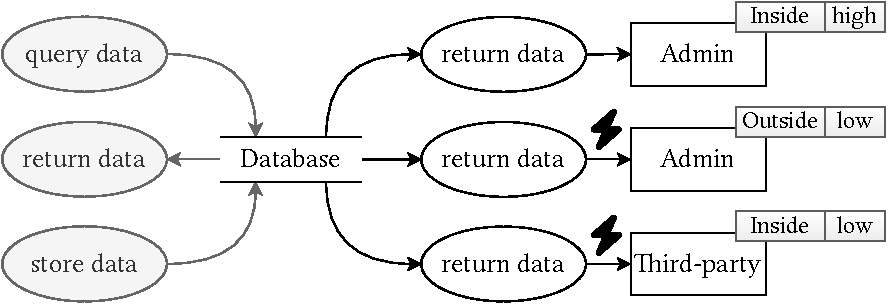
\includegraphics[width=0.95\linewidth]{figures/chapter7/dfd-environmental.pdf}
    \caption{\acf*{DFD} of the extended running example with additional actors and their node labels. Confidentiality violations are marked with lightning bolts.}
    \label{fig:confidentialityanalysis:dfdenvironment}
\end{figure}

We extend the data flow analysis presented in \autoref{sec:confidentialityanalysis:framework} to consider the so-calculated confidence values.
Here, we build on the representation of all confidentiality-related characteristics as data labels and node labels.
As confidence is directly related to such attributes, we extend these characteristics by adding confidence labels. 
\autoref{fig:confidentialityanalysis:dfdenvironment} shows a \ac{DFD} of the extension of our running example with simplified data flows to the actors.
The original data flows from the \emph{Customer} on the left are marked gray.
We add the node labels of the \emph{Admin} actors a third-party actors with their corresponding \emph{confidence} labels \emph{low} and \emph{heigh}.
As discussed previously, these confidence labels originate from the \ac{FIS} based on the input variables from the HSGPS or GPS sensors.
The confidentiality requirement is defined as a data flow constraint that only allows data to flow to actors within the building with \emph{high} confidence.
Thus, the upper data flow is permitted as the \emph{Admin} is inside the building with \emph{high} confidence.
The other data flows show confidentiality violations, as the \emph{Admin} is either outside the building, or a \emph{Third-Party} is considered to be inside the building with only \emph{low} confidence.
Without considering the confidence, the bottom confidentiality violation regarding the \emph{Third-Party} would be missed.

We include all calculated confidence labels in all node and data labels and also in the formulation of data flow constraints.
Although this represents a white-box extension of the data flow analysis, we do not alter the label propagation algorithm, only the textual representation of labels \cite{boltz_handling_2022}.
Thus, the calculation of the \ac{FIS} can be interpreted as a preprocessing step before the data flow analysis.
According to our classification, this represents a \emph{graph-aware} data flow analysis (\level{3}) under uncertainty.
The analysis result contains all information from the data flow analysis, e.g., violation location, violated data flows, and the mismatching labels that cause the violation, including information about the calculated confidence.
Due to the application of \acp{FIS}, information about both the environmental uncertainty sources and their impact is represented within the model and the analysis, as discussed previously.
Last, uncertainty can be analyzed independently on distinct data flows, which minimizes the analysis complexity.
For more information on the realization, please consult our publication \cite{boltz_handling_2022}, or the data set \cite{dataset}.

To conclude this section, we compare and discuss both approaches of uncertainty type-specific data flow analysis.
Both approaches employ already known techniques for representing and handling uncertainty \cite{sobhy_evaluation_2021,troya_uncertainty_2021}, i.e., design space exploration \cite{koziolek_peropteryx_2011,koziolek_automated_2011} or fuzzy inference \cite{klir_fuzzy_1995}.
Both approaches combine these techniques with data flow analysis, either in a black-box manner as in the first approach, or a white-box manner in the second approach.
This results in the first approach for structural uncertainty being \emph{scenario-aware} and the second approach for environmental uncertainty being \emph{graph-aware}.

Both approaches are type-specific and employ techniques that are suited for representing their targeted uncertainty type, i.e., design space exploration for structural uncertainty \cite{sobhy_evaluation_2021,troya_uncertainty_2021}, and fuzzy inference for environmental uncertainty \cite{cheng_fuzzy_2007,esfahani_guidearch_2013,hosmer_using_1992}.
Despite their differences in supported uncertainty types and realization, they show the commonality of considering uncertainty in form of scenarios.
The design decision model of PerOpteryx enables software architects to describe design alternatives, i.e., different scenarios of a software architecture.
The application of \acp{FIS} enables software architects to calculate distinct classes of a \emph{confidence} value, e.g., \emph{low} or \emph{high}, i.e., different scenarios describing the attributes in access control decisions.
The suitability of scenarios or variation \cite{walter_architecture-based_2023} to represent uncertainty has simultaneously been found by \textcite{troya_uncertainty_2021}.
However, besides being type-specific, both approaches also share the shortcoming of requiring expert knowledge.
Software architects or security experts have to instantiate the \ac{FIS} meta model with accurate values or have to specify design decision models.
In the following, we build on these findings to define uncertainty type-agnostic data flow analysis.

\finding{Data flow analysis can be extended by techniques like design space exploration or fuzzy inference to consider uncertainty within the analysis.
Here, decomposing uncertainty sources into their scenarios is expedient.}





\section{Uncertainty Type-Agnostic Data Flow Analysis}%
\label{sec:confidentialityanalysis:typeagnostic}

In this section, we present the second two approaches for uncertainty-aware data flow analysis.
The first approach is \emph{graph-aware} (\level{3}) and the second approach is \emph{impact-aware} (\level{4}), which represents the highest awareness level, see \autoref{sec:confidentialityanalysis:representing}.
Both approaches are type-agnostic, i.e., support all five uncertainty types introduced in \autoref{sec:classification:classification}.
We also present \abunai, which is tooling to support the modeling and analysis of the \emph{impact-aware} approach.
This addresses Problem \PR{3}{3} about type-agnostic data flow analysis.


\subsection{Tracing Uncertainty in Data Flow Analysis}%
\label{sec:confidentialityanalysis:tracing}

Incorporating information about independent data flows---called \acp{TFG} in our terminology introduced in \autoref{sec:confidentialityanalysis:framework}---enables the definition of \emph{graph-aware} analysis (\level{3}).
We present an analysis that traces confidentiality violations back to the originating uncertainty sources using this information.
This enables relating violations to concrete scenarios and simplifies the interpretation and mitigation by software architects.

In this approach, we use variation models \cite{walter_architecture-based_2023,mehl_palladio_2022} to express uncertainty sources and their scenarios.
Variation models are similar to the already discussed design decision models presented in \autoref{sec:confidentialityanalysis:typespecifc}.
Software architects specify target elements and alternative elements of the software architecture.
This can be applied, for instance, to deployment locations, or to actions in \acfp{SEFF}.
As discussed previously, \emph{design uncertainty} is \enquote{normally represented in software models by variability models} \cite{troya_uncertainty_2021}.
Model variation can be used to describe possible outcomes of \emph{Scenario Uncertainty}.
Each uncertainty is represented by a variation point and a selection of alternative architectural elements.
This description results in a variation model \cite{mehl_palladio_2022} of the software architecture.
\autoref{table:confidentialityanalysis:scenarios} shows all scenarios of all uncertainties of the running example.

Based on the variation model, architectural variants can be generated by permutation \cite{mehl_palladio_2022}.
If the information about data flows were ignored, this would cause the same complexity as a \emph{scenario-aware} analysis (\level{2}).
As discussed in \autoref{sec:confidentialityanalysis:representing}, our running example requires $48$ variations.
However, not all uncertainties affect all \acp{TFG}.
Thus, the relevant variations can be filtered in \emph{graph-aware} analysis (\level{3}).
The resulting variants are then analyzed by the data flow analysis presented in \autoref{sec:confidentialityanalysis:framework}.
By relating the resulting confidentiality violations to the analyzed variation and its uncertainty, software architects can focus on critical variants, i.e., variants that violate confidentiality.
The hereby defined analysis traces violations back to their originating uncertainties \cite{bitschi_uncertainty-aware_2022}.

\begin{table}
    \centering
    \begin{tabular}{lll}
        \toprule
        \# & \ac{TFG} name & Relevant uncertainty sources\\
        \midrule
        1 & Request support contact & -  \\
        2 & View available items & \U{3}, \U{4} \\
        3 & Purchase items & \U{1}, \U{2}, \U{3}, \U{4} \\
        \bottomrule
    \end{tabular}
    \caption{Relation of \acfp*{TFG} and uncertainty sources in the running example.}%
    \label{table:confidentialityanalysis:scenariostfgs}
\end{table}

\autoref{table:confidentialityanalysis:scenariostfgs} shows the three \acp{TFG} in the running example and the uncertainty sources that can be found in these \acp{TFG}.
This table can be derived based on \autoref{fig:runningexample:dfd} showing the \ac{DFD} of the running example and \autoref{table:confidentialityanalysis:scenarios} showing the scenarios of all uncertainty sources.
The first \ac{TFG} representing the support contact request is not affected by uncertainty.
The second \ac{TFG} is only affected by the deployment (\U{3}) and the provider trustworthiness (\U{4}).
The third \ac{TFG} is additionally affected by the user input (\U{1}) and the data processing (\U{2}), i.e., by all uncertainties in the running example.

As the three \acp{TFG} are independent, their variations can be analyzed independently.
This results in the lowered complexity of the \emph{graph-aware} analysis (\level{3}) compared to the \emph{scenario-aware} analysis (\level{2}).
Instead of having to apply all possible variations to each \ac{TFG}, we can first filter the relevant uncertainty sources and then only analyze all variations of these uncertainty sources.
Note that this does not affect the identified confidentiality violations as the data flows represented by the \acp{TFG} are independent \cite{seifermann_architectural_2022}.
While the complexity is reduced, the accuracy remains the same.
The more independent data flows there are, the greater this effect becomes, as we assume in real software systems \cite{hahner_architecture-based_2023}.

\begin{algorithm}
    \caption{Algorithm for graph-aware data flow analysis under uncertainty}
    \label{alg:confidentialityanalysis:graphaware}
    \begin{algorithmic}[1]
        \Procedure{\function{analyzeGraphAware}}{$\var{model}, \var{constraint}, \var{uncertainties}$}
            \algindentskip
            \State $\var{violations} \gets \emptyset$
            \State $\var{filtered} \gets \emptyset$
            \State $\var{variations} \gets \function{generateAllVariations}(\var{model}, \var{uncertainties})$
            \State $\var{tfgs} \gets \function{retrieveAllTFGs}(\var{model})$
            \algblockskip

            \For{$\var{tfg} \in \var{tfgs}$} \Comment{Analyze each TFG separately} \label{alg:confidentialityanalysis:graphaware:6}
                \For{$\var{variation} \in \var{variations}$} \Comment{Filter relevant variations}
                    \State $\var{filtered} \gets \var{filtered} \cup \function{filterVariation}(\var{model}, \var{tfg}, \var{variation}, \var{uncertainties})$\label{alg:confidentialityanalysis:graphaware:8}
                \EndFor
                \algblockskip

                \For{$\var{variation} \in \var{filtered}$} \Comment{Only analyze filtered variations}
                    \State $\var{modifiedtfg} \gets \function{applyVariation}(\var{tfg}, \var{variation})$ \label{alg:confidentialityanalysis:graphaware:11}
                    \State $\var{violations} \gets \var{violations} \cup \function{analyze}(\var{modifiedtfg}, \var{constraint})$ 
                \EndFor
            \EndFor
            \algblockskip

            \State \Return{$\var{violations}$}
            \algindentskip
        \EndProcedure   
    \end{algorithmic}
\end{algorithm}

\autoref{alg:confidentialityanalysis:graphaware} shows the algorithm for \emph{graph-aware} data flow analysis (\level{3}).
The approach is similar to \emph{scenario-aware} data flow analysis shown in \autoref{alg:confidentialityanalysis:scenarioaware}, but comprises the aforementioned filtering.
We iterate over all \acp{TFG} of a model in \autoref{alg:confidentialityanalysis:graphaware:6} and analyze each \ac{TFG} separately.
This is possible because \emph{graph-aware} analysis has the information of all data flows.
For each \ac{TFG}, we filter the variations for relevant ones in \autoref{alg:confidentialityanalysis:graphaware:8}.
Afterward, we run the analysis only on these variations.
This is achieved by applying the variation first in \autoref{alg:confidentialityanalysis:graphaware:11} and then forwarding the \ac{TFG} to the data flow analysis.

\begin{algorithm}
    \caption{Algorithm for filtering variations in graph-aware analysis}
    \label{alg:confidentialityanalysis:filtervariation}
    \begin{algorithmic}[1]
        \Procedure{\function{filterVariation}}{$\var{model}, \var{tfg}, \var{variation}, \var{uncertainties}$}
            \algindentskip

            \State $\var{applied} \gets \function{getAppliedUncertainties}(\var{variation, \var{uncertainties})}$ \label{alg:confidentialityanalysis:filtervariation:4}
            \State $\var{vertices} \gets \function{getVertices}(\var{tfg})$ \Comment{Iterate over all vertices}
            \For{$\var{vertex} \in \var{vertices}$} \label{alg:confidentialityanalysis:filtervariation:6}
                \For{$\var{uncertainty} \in \var{applied}$}
                    \If{$\function{affects}(\var{uncertainty}, \var{vertex}, \var{model}, \var{variation})$} \label{alg:confidentialityanalysis:filtervariation:8}
                        \State $\var{applied} \gets \var{applied} \setminus \setted{\var{uncertainty}}$ \label{alg:confidentialityanalysis:filtervariation:9}
                    \EndIf
                \EndFor
                \algblockskip

                \If{$\var{applied} = \emptyset$} \Comment{All uncertainties are relevant}
                    \State \Return{$\setted{\var{variation}}$} \label{alg:confidentialityanalysis:filtervariation:13}
                \EndIf
            \EndFor
            \algblockskip

            \State \Return{$\emptyset$} \label{alg:confidentialityanalysis:filtervariation:17} \Comment{At least one uncertainty is not relevant}
            \algindentskip
        \EndProcedure   
    \end{algorithmic}
\end{algorithm}

\autoref{alg:confidentialityanalysis:filtervariation} shows this filter function.
A variation is relevant for a given \ac{TFG} if all uncertainty sources that cause a change in the architectural model affect at least on vertex of the \ac{TFG}.
We start by retrieving all uncertainties that have been applied in the given variation in \autoref{alg:confidentialityanalysis:filtervariation:4}.
This is the case, if the permutation that causes the variation \cite{mehl_palladio_2022} changes an architectural element due to said uncertainty.
For instance, if one variation only changes architectural elements representing the data processing and the deployment location in our running example, this function would yield the uncertainties \U{2} and \U{3}.
Note that this function is called with \emph{all} possible variations calculated in \autoref{alg:confidentialityanalysis:graphaware}.

Afterward, we iterate over all vertices of the \ac{TFG} in \autoref{alg:confidentialityanalysis:filtervariation:6}.
For each applied uncertainty, we check whether this uncertainty affects the current vertex in \autoref{alg:confidentialityanalysis:filtervariation:8}.
An uncertainty affects a vertex \emph{iff} it causes a variation in an architectural element that is represented by the vertex.
The underlying mapping of the data flow analysis framework presented in \autoref{sec:confidentialityanalysis:framework} is similar to the mapping between architectural models and \acp{DFD} discussed in \autoref{sec:impactanalysis:impactanalysis}.
In our running example, uncertainty in the data processing (\U{2}) affects all vertices in all \acp{TFG} representing this data processing.
If we find such an uncertainty \emph{impact}, we remove the uncertainty from the list of applied uncertainties in \autoref{alg:confidentialityanalysis:filtervariation:9}.

The procedure ends if, at any point in the iteration over all vertices of a \ac{TFG}, the list of applied uncertainties gets empty.
This is the case if all uncertainties considered in the given variation are relevant to the \ac{TFG}.
Thus, the variation is relevant for the \emph{graph-aware} analysis and is returned in \autoref{alg:confidentialityanalysis:filtervariation:13}.
If not all uncertainties that have been varied are relevant, an empty set is returned instead in \autoref{alg:confidentialityanalysis:filtervariation:17}.

We explain the interplay of \autoref{alg:confidentialityanalysis:graphaware} and \autoref{alg:confidentialityanalysis:filtervariation} based on the the three \acp{TFG} of our running example, shown in \autoref{table:confidentialityanalysis:scenariostfgs}.
Here, the analyzing the first \ac{TFG} representing the support contact request and the last \ac{TFG} representing the item purchase are the edge cases of the filter algorithm.
The first \ac{TFG} has no relevant uncertainty source.
Thus, \autoref{alg:confidentialityanalysis:filtervariation} always returns an empty list except for the single variation, where no uncertainty is applied.
In this case, \autoref{alg:confidentialityanalysis:filtervariation:8} trivially evaluates to \emph{true} as the list already was empty.
The third \ac{TFG} is affected by all four uncertainty sources \U{1} -- \U{4}.
Thus, every permutation of the uncertainties creates a variation that is relevant for the \ac{TFG} and the filter has no effect.
Regarding the second \ac{TFG}, only four variations are relevant, i.e., the variations that represent the scenarios of Uncertainty \U{3} and Uncertainty \U{4}, \autoref{table:confidentialityanalysis:scenariostfgs}.
Only these variations are returned by the filter algorithm and analyzed using the data flow analysis.
This also again shows the reduced complexity of the \emph{graph-aware} analysis (\level{3}), as for most \acp{TFG} in the running example, not all variations are relevant.

The information about uncertainty sources, filtered variations, \acp{TFG}, and confidentiality violations enables the tracing approach.
For each confidentiality violation, we can store the related \ac{TFG} and which variation has been applied in the analysis process.
The reference to the variation provides the knowledge about considered uncertainty sources and their properties.
This represents the information categories \textbf{1.} -- \textbf{8.} from \autoref{table:confidentialityanalysis:informationcategories}.
Combined, this provides software architects with comprehensive knowledge to better understand the origin of the confidentiality violations and to apply appropriate measures.

\begin{figure}
    \centering
    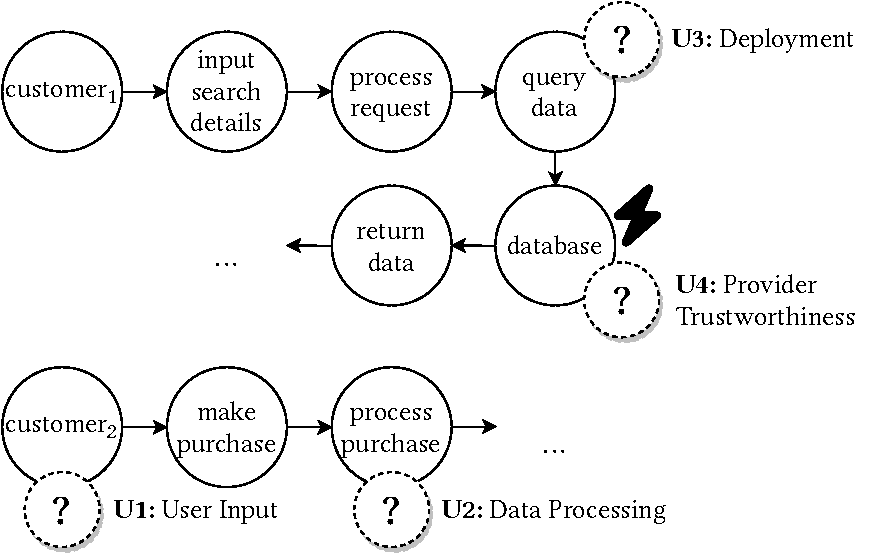
\includegraphics[width=0.95\linewidth]{figures/chapter7/uncertaintytracing.pdf}
    \caption{Excerpts of two \acfp*{TFG} from the running example with annotated uncertainty impacts and a confidentiality violation, marked with a lightning bolt.}
    \label{fig:confidentialityanalysis:uncertaintytracing}
\end{figure}

We illustrate this with one variation of the uncertainty sources of the running example.
\autoref{fig:confidentialityanalysis:uncertaintytracing} shows excerpts of the \acp{TFG} that represent the querying of items and the making of purchases.
The annotated uncertainty represents the impact of the uncertainty due to changes in the architectural model.
For instance, in this variation, the deployment location is the \emph{Cloud Service} and the provider is classified as \emph{Suspicious}, see \autoref{table:confidentialityanalysis:scenarios}.
This uncertainty would cause a confidentiality violation when the data is stored in the database, as marked with the lightning bolt.
As discussed with \autoref{table:confidentialityanalysis:scenariostfgs}, this represents one of the $48$ possible variations.
This confidentiality violation can thus be traced back to the uncertainties \U{3} and \U{4}.
The tracing follows the data flow in inverse direction, and could thus be interpreted as a reverse uncertainty impact analysis.
The graphical representation of the \acp{TFG} in \autoref{fig:confidentialityanalysis:uncertaintytracing} also shows the independence to the other uncertainty sources, e.g., \U{1}, and \U{2}.
They affect other vertices of another \ac{TFG} and can thus be safely ignored when interpreting the confidentiality violation in the upper \ac{TFG}.
This benefits the understanding of software architects and simplifies both further analyses and the mitigation.

\emph{Graph-aware} data flow analysis (\level{3}) minimizes the analysis complexity while enhancing the expressiveness of the analysis results.
As the presented approach for tracing uncertainty builds on variation modeling \cite{mehl_palladio_2022,walter_architecture-based_2023}, any architectural element can be varied.
This enables an uncertainty type-agnostic approach.
However, this approach has two major shortcomings.
First, variation modeling still requires some expert knowledge from the software architects.
Although they do not have to manually model the variations or alter the \acp{DFD} by hand, they have to specify the correct variation types and variation points.
This requires them to understand which variation points match the uncertainty sources they want to analyze.
Failing to accurately represent the uncertainty in the variation model can impair or even void the analysis results \cite{hahner_arcn_2024}.
This discussion is similar to the extension of the uncertainty impact analysis shown in \autoref{sec:impactanalysis:awareness}.

Second, the approach ignores uncertainty interactions.
For instance, if the \emph{Database Service} is deployed on-premise, Uncertainty \U{4} about the provider's trustworthiness has no effect.
Because the uncertainty filter presented in \autoref{alg:confidentialityanalysis:filtervariation} does not consider this, more varied \acp{TFG} are analyzed than required.
In this example, the variation of a \emph{suspicious} cloud provider and a deployment \emph{on premise} can be safely ignored as there would be no data flow to the cloud provider in the first place.
This marks the difference between a \emph{graph-aware} analysis (\level{3}) and an \emph{impact-aware} analysis (\level{4}).
The difference becomes visible when comparing \autoref{fig:classification:dag} with \autoref{fig:confidentialityanalysis:uncertaintytracing}.
The former shows uncertainty as part of the \ac{DFD} while the latter only considers changes in architectural elements that are related to \ac{DFD} nodes.
Generating and filtering variations cannot represent transitive effects of uncertainty impacts within a \ac{DAG}.
To address this, we consider uncertainty as a first-class concern in the data flow analysis, creating an \emph{impact-aware} analysis (\level{4}).

\finding{Considering \acfp{TFG} in the confidentiality analysis of uncertainty scenario combinations surpasses the analysis capabilities of analyses that only consider all possible variations.
Still, the resulting analysis is limited by the expressiveness of variation modeling.
To overcome this limitation regarding the transitive impact, uncertainty has to be presented as first-class concern within \acfp{DFD} and the data flow analysis.}


\subsection{Impact-Aware Data Flow Analysis Under Uncertainty}%
\label{sec:confidentialityanalysis:abunai}

More than a decade ago, \textcite{garlan_software_2010} proposed to consider uncertainty as a first-class concern in software engineering.
We follow this proposal to define the last approach of this chapter, an uncertainty type-agnostic and \emph{impact-aware} data flow analysis (\level{4}).
First, we present a meta model for representing uncertainty sources as part of the architectural model.
This addresses the shortcoming regarding expert knowledge of variation modeling \cite{mehl_palladio_2022,walter_architecture-based_2023,hahner_model-based_2023}.
Afterward, we introduce the notion of a \acf{NDFD} \cite{hahner_classification_2023} that incorporates uncertainty as a first-class entity within the \ac{DFD}.
We discuss how to analyze such \acp{NDFD} and handle simple uncertainty interactions in \acp{DAG} while identifying confidentiality violations.
Last, we present our tooling \abunai that comprises uncertainty modeling and automated analysis support.

In presenting the previous approaches for analyzing structural uncertainty and environmental uncertainty, and tracing uncertainty, we discussed different approaches to express uncertainty as part of the architectural model.
This includes design decision models \cite{koziolek_peropteryx_2011,koziolek_automated_2011,walter_architectural_2022}, \acp{FIS} \cite{klir_fuzzy_1995,boltz_handling_2022}, and variation modeling \cite{mehl_palladio_2022,hahner_model-based_2023}.
They share the common shortcoming of requiring expert knowledge to bridge the gap between identifying uncertainty sources and expressing them as part of the software architecture.
We close this gap by providing a meta model that connects the five uncertainty types presented in \autoref{ch:classification} to the architectural model.
This approach is similar to the modeling of uncertainty for impact analysis presented in \autoref{sec:impactanalysis:representing}, where we already addressed a similar issue.

\begin{figure}
    \centering
    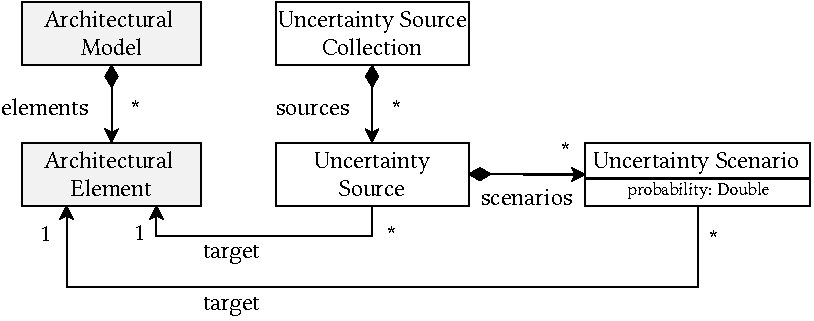
\includegraphics[width=0.95\linewidth]{figures/chapter7/abunai-metamodel.pdf}
    \caption{Overview of the meta model for expressing uncertainty sources and scenarios in architectural models. Existing elements of the software architecture are highlighted gray.}
    \label{fig:confidentialityanalysis:uncertaintymetamodel}
\end{figure}

\autoref{fig:confidentialityanalysis:uncertaintymetamodel} shows the meta model for modeling uncertainty sources and scenarios as part of the software architecture.
We use the same terminology as the uncertainty classification presented in \autoref{ch:classification}, i.e., uncertainty sources and scenarios, instead of design decisions, or variations.
To introduce this meta model, we only refer to the concept of an \emph{Architectural Model}, which comprises any number of \emph{Architectural Elements}.
Software architects define an \emph{Uncertainty Source Collection} alongside the architectural model.
This collection consists of \emph{Uncertainty Sources} that consist of \emph{Uncertainty Scenarios}.
Each source references one \emph{Architectural Element}, which represents its default scenario.
Until this point, the software architecture is annotated with uncertainty sources like in the uncertainty impact analysis, see \autoref{ch:impactanalysis}.
We extend this annotation by modeling any number of \emph{Uncertainty Scenario} that also refer to one \emph{Architectural Element}.
These scenarios represent alternative scenarios of the \emph{Uncertainty Source} any can additionally have a probability.

\begin{figure}
    \centering
    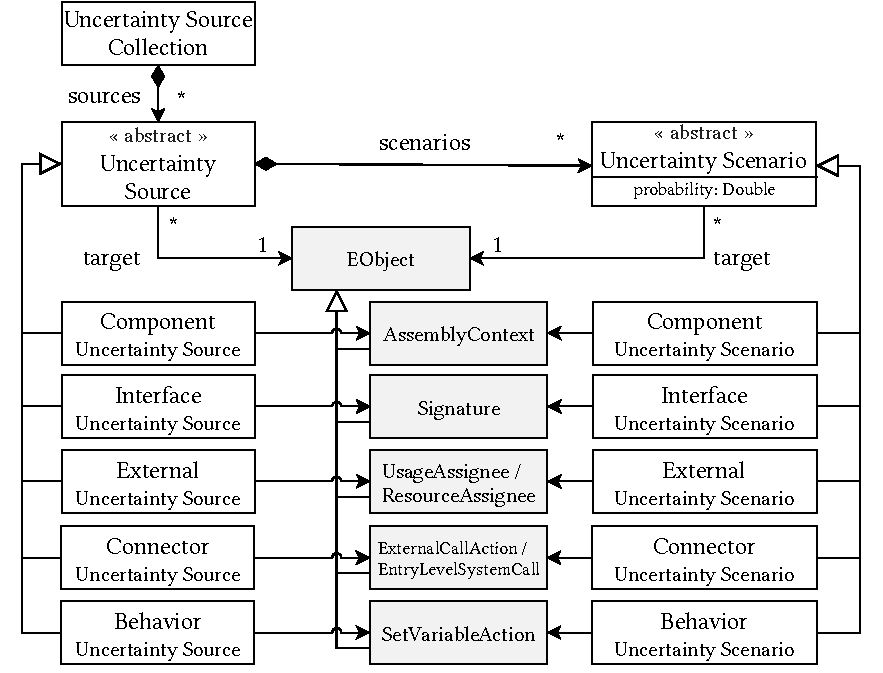
\includegraphics[width=\linewidth]{figures/chapter7/abunai-metamodel-pcm.pdf}
    \caption{Meta model of uncertainty sources and scenarios in the \acf*{PCM}.}
    \label{fig:confidentialityanalysis:uncertaintymetamodelpcm}
\end{figure}

Depending on the type of modeled uncertainty, see \autoref{table:classification:classification:type}, software architects can refine the model.
\emph{Recognized Ignorance} is modeled as an \emph{Uncertainty Source} that references an \emph{Architectural Element}.
\emph{Scenario Uncertainty} is modeled as a \emph{Uncertainty Source} with any number of \emph{Uncertainty Scenarios} that also reference \emph{Architectural Elements}.
\emph{Statistical Uncertainty} is modeled by enriching the \emph{Uncertainty Scenarios} with probabilities between 0 and 1.
We require that all probabilities add up to 1.
The probability of the default scenario expressed by the \emph{Uncertainty Source} is 1 minus the sum of the probabilities of all of its scenarios.
However, providing probabilities is optional, the field can be left empty to describe \emph{Scenario Uncertainty}.
Depending on the available information, all options of the category \emph{Uncertainty Type} presented in \autoref{sec:classification:classification} can be modeled and mixed.
In our running example, Uncertainty \U{4} is modeled by creating an \emph{Uncertainty Source} that refers to the \emph{Cloud Service's} trustworthiness with the alternative \emph{Uncertainty Scenario} of being suspicious, see \autoref{table:confidentialityanalysis:scenarios}.
A high level of trust in the provider can be expressed, for example, by a probability of 0.1 for the alternative scenario of a suspicious provider.

We extend this meta model and apply it to the \ac{PCM}, thereby replacing the \emph{Architectural Elements} of \autoref{fig:confidentialityanalysis:uncertaintymetamodel} with concrete \ac{PCM} element types.
\autoref{fig:confidentialityanalysis:uncertaintymetamodelpcm} shows the resulting meta model.
We simplify some of the elements for the sake of clarity, e.g. by combining \emph{UsageAssignees} and \emph{ResourceAssignees}, which are modeled separately.
Similarly to the overview, a \emph{Uncertainty Source Collection} contains any number of \emph{Uncertainty Sources} that contain any number of \emph{Uncertainty Scenarios}.
Both the \emph{Uncertainty Source} and the \emph{Uncertainty Scenario} target exactly one architectural element.
Because the \ac{PCM} is based on the \acf{EMF}, the common super type is \emph{EObject}.

The five uncertainty types of the category \emph{Architectural Element Type}, see \autoref{table:classification:classification:architecturalelementtype}, have their corresponding uncertainty sources and uncertainty scenarios.
All sources inherit from the abstract \emph{Uncertainty Source} and all scenarios from the abstract \emph{Uncertainty Scenario}, respectively.
For the sake of clarity, we leave out details like the inherited \emph{probability} field and the \emph{scenarios} relation between all sub types.
All sources and scenarios target an \ac{PCM} element type, e.g., \emph{Component Uncertainty Sources} and \emph{Component Uncertainty Scenarios} target \ac{PCM} \emph{AssemblyContexts}.
This ensures valid model instances, as both sources and scenarios are required to reference the same \ac{PCM} element type, e.g., different \emph{AssemblyContexts}, or \emph{Signatures}.
Some types of \emph{Uncertainty Sources} and \emph{Uncertainty Scenarios} can refer to more than one \ac{PCM} element, e.g., \emph{Connector} uncertainty, and \emph{External} uncertainty.
In our implementation of this meta model \cite{dataset}, we realize this using sub types of \emph{Connector} uncertainty and \emph{External} uncertainty, respectively, to ensure type safety.
Note that the referenced \ac{PCM} elements are slightly different compared to the annotated elements of uncertainty impact analysis, as discussed in \autoref{sec:impactanalysis:representing}.

\begin{table}
    \begin{tabularx}{\linewidth}{lllX}
        \toprule
        \# & Uncertainty type & Source target \ac{PCM} element & Alternative scenario targets \\
        \midrule
        \U{1} & Connector & \emph{BuyEntryLevelSystemCall} & 
            \mtl{\emph{ErroneousEntryLevelSystemCall}\\\emph{MaliciousEntryLevelSystemCall}} \\
        \U{2} & Behavior & \emph{UserDataProcessing} & 
            \mtl{\emph{BrokenEncryptionProcessing}\\\emph{BrokenValidationProcessing}\\\emph{EverythingBrokenProcessing}} \\
        \U{3} & Component & \emph{DatabaseServiceOnPremise} & \emph{DatabaseServiceInCloud} \\
        \U{4} & External & \emph{ProviderTrusted} & \emph{ProviderSuspicious} \\
        \bottomrule
    \end{tabularx}
    \caption{Modeling the uncertainty sources and their scenarios in the running example.}%
    \label{table:confidentialityanalysis:uncertaintymodelrunningexample}
\end{table}

We apply this meta model to our running example to illustrate it with all uncertainty sources \U{1} -- \U{4}.
\autoref{table:confidentialityanalysis:uncertaintymodelrunningexample} shows the targeted elements of all uncertainty sources and also the targeted elements of alternative scenarios.
Thereby it realizes the scenarios \autoref{table:confidentialityanalysis:scenarios} and connects this collection to a concrete architectural model described based on the \ac{PCM}.
The restriction to concrete architectural elements simplifies the modeling of uncertainty sources and their scenarios and also minimizes the risk of an erroneous specification.
Compared to, e.g., variation modeling \cite{mehl_palladio_2022,walter_architecture-based_2023}, this bridges the gap between the classification of software-architectural uncertainty and the software architecture.

\finding{Modeling uncertainty sources and uncertainty scenarios that reference elements of the architectural model connects the classification of software-architectural uncertainty to architectural models.
This provides the foundation for analyzing uncertainty as first-class entity in software architecture.}

To consider uncertainty not only as first-class entity within the software architecture but also in architecture-based data flow analysis, we need means to represent the impact in \acp{DFD}.
To this end, we discussed the mapping and the representation of uncertainty to \acp{DFD} and \acp{DAG} in \autoref{sec:classification:dfd}.
We also introduced the notion of \emph{primary} uncertainty that affects vertices and \emph{secondary} uncertainty that affects edges.
By connecting this notion to the previously introduced meta model for modeling uncertainty sources and scenarios, we are able to define an \emph{impact-aware} data flow analysis (\level{4}).
Uncertainty is sometimes defined as \enquote{any departure from the unachievable ideal of complete determinism} \cite{walker_defining_2003}, see \autoref{sec:foundations:uncertainty}.
We build on this idea by describing the lack of determinism and define the notion of \acfp{NDFD}.
Put simply, we extend \acfp{DFD} to incorporate uncertainty as first-class entity that is represented by nondeterminism.
Here, we also benefit from the comprehensive foundations regarding the representation of the impact of uncertainty in \ac{DFD}, provided in \autoref{sec:impactanalysis:representing}.

\begin{figure}
    \centering
    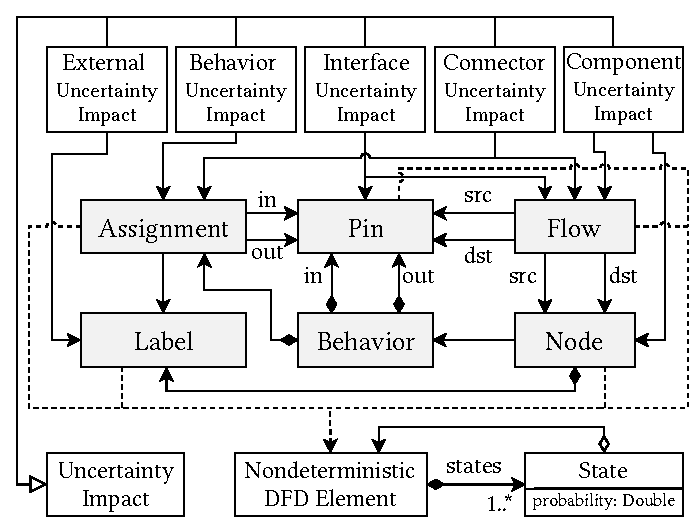
\includegraphics[width=0.8\linewidth]{figures/chapter7/ndfd.pdf}
    \caption{Meta model of \acfp*{NDFD}.}
    \label{fig:confidentialityanalysis:ndfd}
\end{figure}

\autoref{fig:confidentialityanalysis:ndfd} shows the meta model of \acp{NDFD}, thereby extending the meta model of \acp{DFD} with uncertainty impacts shown in \autoref{fig:impactanalysis:representing:metamodel}.
Every \ac{DFD} element originating from the unified modeling primitives \cite{seifermann_unified_2021} and highlighted in gray represents a \emph{Nondeterministic Data Flow Diagram Element}.
Such an element has one or more \emph{States} that reference the element, or other elements.
Trivially, an element with only one \emph{State} that references the element itself represents determinism.
Thus, every \ac{DFD} is also a valid \ac{NDFD}, which lacks nondeterminism, i.e., uncertainty.
Uncertainty is represented by multiple \emph{States} that can additionally have a \emph{probability}.
Regarding the probability, the same rules apply as for the meta model for uncertainty and scenarios in the architectural model.

This meta model enables the concise representation of uncertainty in \acp{DFD}.
For instance, Uncertainty \U{4} about the provider trustworthiness represents \emph{External} uncertainty.
It can be expressed by an nondeterministic \emph{Label} with two states: \emph{Trustworthy} and \emph{Suspicious}.
The same applies to the other uncertainty sources, e.g., Uncertainty \U{2} about the processing can be represented by multiple alternative \emph{Assignments}.

We reuse the mapping of uncertainty sources to impact locations within the \ac{DFD} from \autoref{sec:classification:dfd}, and the mapping of \ac{PCM} models to \acp{DFD} presented in \autoref{sec:confidentialityanalysis:framework}.
Additionally, every \emph{Uncertainty Scenario} from the meta model presented in \autoref{fig:confidentialityanalysis:uncertaintymetamodelpcm} is mapped to a \emph{State} of the \ac{NDFD} meta model.
The state representing the default scenario of the \emph{Uncertainty Source} references the \ac{DFD} element itself.
All alternative scenarios reference the \ac{DFD} elements that represent the targeted architectural elements of these scenarios.
The probability of a \emph{State} corresponds to the probability of the \emph{Uncertainty Scenario}.

We can apply this mapping to the modeled uncertainty sources and uncertainty scenarios of the running example, shown in \autoref{table:confidentialityanalysis:uncertaintymodelrunningexample}.
The \emph{EntryLevelSystemCall} that is referenced by Uncertainty \U{1} is mapped to a nondeterministic \ac{DFD} element and referenced by the default state of this element.
The \ac{DFD} element has additional states to also represent erroneous and malicious user input.
Because Uncertainty \U{1} represents \emph{Connector} uncertainty, the nondeterministic \ac{DFD} elements are flows and assignments that set the labels for valid, erroneous, or malicious input.
However, due to the uncertainty, we cannot know which assignment is applied, i.e., nondeterminism.

\finding{\acfp{NDFD} consist of all \acfp{DFD} elements, which have one or multiple states.
These states represent uncertainty as a first-class concern in modeling and data flow analysis.}

The concept of states in \acp{NDFD} can be transferred to \acp{DAG}.
This enables the application of the data flow analysis that operates on \acp{TFG}, which are \acp{DAG}.
Here, we use the notion of \emph{primary} and \emph{secondary} uncertainty.
As discussed in \autoref{sec:classification:dfd}, the five uncertainty types can be represented by either \emph{primary} or \emph{secondary} uncertainty.
\emph{Component} uncertainty, \emph{Connector} uncertainty, and \emph{Interface} uncertainty affect the data flow, i.e., the edges of a \ac{DAG}.
\emph{External} uncertainty and \emph{Behavior} uncertainty affect nodes, i.e., the vertices of a \ac{DAG}.
We use this mapping of the elements of a \ac{DFD}---that are also elements of a \ac{NDFD}---to simplify the data flow analysis.
In mapping \ac{PCM} elements to \acp{TFG}, we map the uncertainty sources and scenarios to \emph{primary} and \emph{secondary} uncertainty.
The resulting \ac{DAG} with these uncertainties represents a \ac{NDFD} and comprises uncertainty as a first-class entity.
To repeat from \autoref{sec:classification:dfd}, a \ac{DAG} $G = (V, E)$ consists of vertices $V$ and edges $E$.
All \emph{primary} uncertainty impacts form a subset of all vertices $V_{u} \subseteq V$.
All \emph{secondary} uncertainty impacts form a set $E_{u} = \setted{E_{u_{1}}, \dots, E_{u_{n}}}$, where each set comprises alternative edges.

\begin{figure}
    \centering
    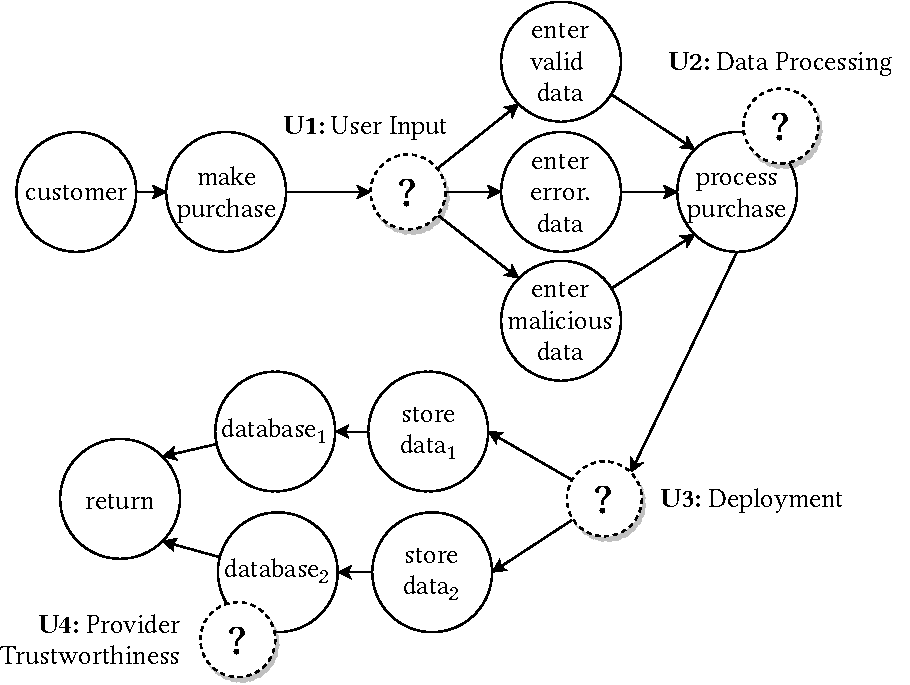
\includegraphics[width=0.9\linewidth]{figures/chapter7/lastdag.pdf}
    \caption{\acf*{DAG} of the \acf*{TFG} representing the item purchase in the running example, with primary and secondary uncertainty, denoted by question marks.}
    \label{fig:confidentialityanalysis:dag}
\end{figure}

The first \ac{TFG} of the support contact request contains no uncertainty and is thus not relevant, see \autoref{table:confidentialityanalysis:scenariostfgs}.
The \ac{DAG} of the second \ac{TFG} is shown while discussing \emph{primary} and \emph{secondary} uncertainty in \autoref{fig:classification:dag}.
To make the list of \acp{DAG} of the running example complete, \autoref{fig:confidentialityanalysis:dag} shows the \ac{DAG} of the third \ac{TFG} of the running example, which represents the purchase of items.
This \ac{DAG} contains all four uncertainties \U{1} -- \U{4}.

The \emph{secondary} uncertainties are shown as alternative edges.
As discussed above, the \emph{Connector} uncertainty of the user input (\U{1}) and the \emph{Component} uncertainty of the deployment (\U{3}) represent \emph{secondary} uncertainty.
The \emph{primary} uncertainties are annotated to vertices.
The \emph{Behavior} uncertainty of the data processing (\U{2}) and the \emph{External} uncertainty of the provider trustworthiness (\U{4}) represent \emph{primary} uncertainty.
The scenarios of the \emph{secondary} uncertainty are visible in the graphical representation of the \ac{DAG}, e.g., the alternative types of user input in Uncertainty \U{1}.
The scenarios of \emph{primary} uncertainty are hidden in this view, because they affect \ac{DFD} elements that are represented by the vertices, e.g., the \emph{Label} of the \emph{database\textsubscript{2}} being \emph{Trustworthy}, or \emph{Suspicious}.
Here, we refer to \autoref{sec:confidentialityanalysis:framework} for our introduction on \acp{TFG} and their relation to \acp{DAG}.

The \ac{TFG} shown in \autoref{fig:classification:dag} is also suitable to illustrate the mapping from an architectural model with uncertainty sources and scenarios to \acp{NDFD} and \acp{DAG}.
\autoref{table:confidentialityanalysis:uncertaintymodelrunningexample} shows three different scenarios regarding Uncertainty \U{1} of the user input.
As this is \emph{Connector} uncertainty and modeled with three alternative \emph{EntryLevelSystemCalls}, the resulting \ac{DAG} also comprises the corresponding vertices, e.g., \emph{enter valid data} and \emph{enter malicious data}, with a \emph{secondary} uncertainty.
In the \ac{NDFD}, this is represented by a nondeterministic element with three states, which translates to this part of the \ac{DAG}.
The same applies to Uncertainty \U{3} with the two deployment options.
The \emph{primary} uncertainties \U{2} and \U{4} have been discussed in the previous paragraph.
Here, the scenarios are not visible in the \ac{DAG}, because it only represents the \emph{Nodes} of an \ac{NDFD} as vertices, and \emph{primary} uncertainty affects these vertices.
Nevertheless, the label propagation presented in \autoref{sec:confidentialityanalysis:framework}, is presented with alternative \ac{DFD} elements, e.g., alternative \emph{Assignments} representing the data processing alternatives in Uncertainty \U{2}.
In sum, the notion of \acp{TFG} remains suitable to model and analyze \ac{DAG}, also under uncertainty.

We build on this representation of \acp{NDFD} as \emph{primary} and \emph{secondary} uncertainty in \acp{DAG} to define \emph{impact-aware} data flow analysis (\level{4}).
Based on this discussion, differentiating between the different analyses is straightforward.
\emph{Scenario-aware} data flow analysis (\level{2}) iterates over all scenarios, without considering \acp{TFG}, as shown in \autoref{alg:confidentialityanalysis:scenarioaware}.
\emph{Graph-aware} data flow analysis (\level{3}) iterates over all \acp{TFG}, without considering uncertainty affecting individual vertices, as shown in \autoref{alg:confidentialityanalysis:graphaware}.
\emph{Impact-aware} data flow analysis (\level{4}) iterates over vertices and considers uncertainty as a first-class entity in the analysis process.
This again reduces the number of \acp{TFG} that have to be analyzed, and it enables the consideration of the transitive impact of uncertainty and uncertainty interactions.

\begin{algorithm}
    \caption{Algorithm for impact-aware data flow analysis under uncertainty}
    \label{alg:confidentialityanalysis:impactaware}
    \begin{algorithmic}[1]
        \Procedure{\function{analyzeImpactAware}}{$\var{model}, \var{constraint}, \var{uncertainties}$}
            \algindentskip
            \State $\var{violations} \gets \emptyset$
            \State $\var{input} \gets \function{retrieveAllTFGs}(\var{model})$
            \State $\var{output} \gets \emptyset$
            \algblockskip

            \For{$\var{tfg} \in \var{input}$} \Comment{Processing of all uncertainties}
                \State $\var{sources} \gets \function{getSources}(\var{tfg})$ \Comment{Start the evaluation at each source}
                \For{$\var{source} \in \var{sources}$}
                    \State $\var{output} \gets \var{output} \cup \function{processVertex}(source, uncertianties, \setted{\var{tfg}})$\label{alg:confidentialityanalysis:impactaware:8}
                \EndFor
            \EndFor
            \algblockskip

            \For{$\var{tfg} \in \var{output}$} \Comment{Confidentiality analysis on the resulting TFGs}
                \State $\var{violations} \gets \var{violations} \cup \function{analyze}(\var{tfg}, \var{constraint})$\label{alg:confidentialityanalysis:impactaware:12}
            \EndFor
            \algblockskip

            \State \Return{$\var{violations}$} \label{alg:confidentialityanalysis:impactaware:14}
            \algindentskip
        \EndProcedure   
    \end{algorithmic}
\end{algorithm}

\begin{algorithm}
    \caption{Algorithm for processing vertices with primary and secondary uncertainty}
    \label{alg:confidentialityanalysis:processvertex}
    \begin{algorithmic}[1]
        \Procedure{\function{processVertex}}{$\var{vertex}, \var{uncertainties}, \var{tfgs}$}
            \algindentskip

            \If{$\function{isInPrimaryUncertaintySet}(\var{vertex}, \var{uncertainties})$} \label{alg:confidentialityanalysis:processvertex:2}
                \For{$\var{state} \in \function{getStates}(\var{vertex}, \var{uncertainties})$}
                    \For{$\var{tfg} \in \var{tfgs}$}
                        \State $\var{newtfg} \gets \function{applyPrimaryUncertainty}(\var{vertex}, \var{state}, \var{tfg})$
                        \State $\var{tfgs} \gets \var{tfgs} \cup \setted{\var{newtfg}}$
                    \EndFor
                \EndFor
            \EndIf
            \algblockskip

            \For{$\var{edge} \in \function{getOutgoingEdges}(\var{vertex})$} \label{alg:confidentialityanalysis:processvertex:10}
                \If{$\function{isInSecondaryUncertaintySet}(\var{edge}, \var{uncertainties})$}
                    \For{$\var{tfg} \in \var{tfgs}$}
                        \State $\var{newtfg} \gets \function{applySecondaryUncertainty}(\var{vertex}, \var{edge}, \var{tfg})$ \label{alg:confidentialityanalysis:processvertex:13}
                        \State $\var{tfgs} \gets \var{tfgs} \cup \setted{\var{newtfg}}$
                    \EndFor
                \EndIf
            \EndFor

            \For{$\var{successor} \in \function{getSuccessors}(\var{vertex})$}
                \State $\var{tfgs} \gets \var{tfgs} \cup \function{processVertex}(\var{successor}, \var{uncertainties}, \var{tfgs})$ \label{alg:confidentialityanalysis:processvertex:19}
            \EndFor
            \algblockskip

            \State \Return{$\var{tfgs}$}
        \EndProcedure   
    \end{algorithmic}
\end{algorithm}

\autoref{alg:confidentialityanalysis:impactaware} shows the \emph{impact-aware} data flow analysis.
It consists of two steps.
First, all uncertainties in all \ac{TFG} are processed.
By following the flow of data starting from each source, every impact of uncertainty has to be considered in the processing in \autoref{alg:confidentialityanalysis:impactaware:8}.
We start at the sources because uncertainty follows the flow of data, as found in \autoref{sec:impactanalysis:dfdpropagation}.
Thus, processing the impact of uncertainty in this direction simplifies the analysis.
The resulting \acp{TFG} are input to the confidentiality analysis in \autoref{alg:confidentialityanalysis:impactaware:12}.
This analysis is executed separately on every resulting, independent \ac{TFG}.
The collected violations are returned in \autoref{alg:confidentialityanalysis:impactaware:14}.
\autoref{alg:confidentialityanalysis:processvertex} shows the processing of \emph{primary} and \emph{secondary} uncertainty in \emph{impact-aware} data flow analysis.
Put simply, instead of combining all possible scenarios of all uncertainties (\level{2}), or all scenarios on one \ac{TFG} (\level{3}), we recursively apply only the scenarios that have an actual impact on each other (\level{4}).
The \emph{processVertex} function is called with a vertex, initially the source of a \ac{TFG}, all uncertainties, and a set of \acp{TFG}, initially only the \ac{TFG} itself.

We first handle \emph{primary} uncertainty, starting in \autoref{alg:confidentialityanalysis:processvertex:2}.
If the vertex is in the set of vertices affected by \emph{primary} uncertainty $V_{u} \subseteq V$, we apply every state from the \ac{NDFD} to every \ac{TFG} in the set, thereby creating and adding new \acp{TFG}.
Due to the set semantics, the original \ac{TFG} representing the default scenario is not contained twice.
For instance, the \emph{primary} uncertainty \U{2} with 4 scenarios---and thus, 4 states of the \ac{NDFD} element---causes 4 new \ac{TFG}.
Afterward, we handle \emph{secondary} uncertainty, starting in \autoref{alg:confidentialityanalysis:processvertex:10}.
Here, we filter all outgoing edges for those that are in the set of secondary uncertainty sets, i.e., edges in one $E_{u_{i}} \in E_{u}$.
For every identified, outgoing edge, we apply the uncertainty to all \acp{TFG} in \autoref{alg:confidentialityanalysis:processvertex:13}, thereby creating copies of all \acp{TFG} with only one of the outgoing edges in $E_{u_{i}}$.
For instance, the \emph{secondary} uncertainty \U{1} with 3 states as shown in \autoref{fig:confidentialityanalysis:dag} causes three copies per \ac{TFG}, with only one outgoing edge from the \emph{make purchase} vertex.

Last, we continue with all successors of the analyzed vertex until a sink is reached.
Because this recursive call to the \emph{processVertex} function in \autoref{alg:confidentialityanalysis:processvertex:19} contains the current set of \acp{TFG}, the transitive impact of uncertainty is considered.
Note that the realization of this algorithm in our data set \cite{dataset} comprises optimizations of this algorithm, similar to the algorithms shown in \autoref{sec:impactanalysis:pcmpropagation}.
In our exemplary \ac{DAG} shown in \autoref{fig:confidentialityanalysis:dag}, this results in a lower number of resulting \acp{TFG} compared to \emph{graph-aware} analysis (\level{3}).
After the processing of the vertex \emph{process purchase}, we have 12 \acp{TFG}, caused by the 3 scenarios of Uncertainty \U{1} times the 4 scenarios of Uncertainty \U{4}.
However, after evaluating Uncertainty \U{3}, only the lower branch is affected by Uncertainty \U{4}.
Thus, this uncertainty is only applied to those \acp{TFG} that represent the state where the data flows to this branch instead of to all \acp{TFG}.
To achieve this, we have to consider the transitive effect of uncertainty in the analysis, which requires the representation of uncertainty as first-class entity.

\finding{Representing \acfp{NDFD} as \acfp{DAG} with uncertainty as a first-class entity enables the consideration of transitive effects of uncertainty and interactions of uncertainty sources.
Additionally, the analysis scalability is enhanced because the number of required \acfp{TFG} is reduced.}

In the introduction of this chapter, we highlighted the need for automated confidentiality analysis.
We realize the concept of an \emph{impact-aware} data flow analysis based on the framework presented in \autoref{sec:confidentialityanalysis:framework}.
Our tooling \abunai provides modeling support for software architects and an automated, uncertainty \emph{impact-aware} analysis of confidentiality.
The implementation is part of the data set \cite{dataset}.

Similarly to the tool support for uncertainty impact analysis, we build on the Palladio tooling \cite{reussner_modeling_2016,reussner_palladio_2024} that offers a meta model, the \ac{PCM}, and graphical editor support.
Our Java-based open-source implementation realizes the algorithms presented above.
The analysis requires a \ac{PCM} model and an uncertainty model that comprises uncertainty sources and scenarios as input.
Our implementation is closely oriented to the meta model shown in \autoref{fig:confidentialityanalysis:uncertaintymetamodelpcm}.
The analysis provides a number of helpful outputs for software architects.
Besides identifying confidentiality violations, combinations of uncertainty scenarios can be generated, compared, and related to the violations.
This includes calculating the overall probability by multiplying the probability of analyzed uncertainty scenarios.
Additionally, metrics regarding the analysis complexity are shown.
It is also possible to build on the generated \acp{TFG} to create further analyses or end-to-end approaches \cite{weyns_towards_2023}.
We showcase \abunai based on the running example in \autoref{sec:appendix:confidentiality}.

\finding{The uncertainty impact-aware analysis of confidentiality can be fully automated based on the \acf{PCM} and the existing tooling of the Palladio approach.
Uncertainty sources and scenarios are modeled as first-class entities within the software architecture and analyzed while considering the transitive impact of uncertainty and uncertainty interactions.
The resulting analysis can be used for the creation of end-to-end approaches.}





\section{Complexity of Data Flow Analysis Under Uncertainty}%
\label{sec:confidentialityanalysis:complexity}

Throughout this chapter, we discussed the complexity and scalability of the different approaches for data flow analysis under uncertainty, i.e., \emph{scenario-aware} analysis (\level{2}), \emph{graph-aware} analysis (\level{3}), and \emph{impact-aware} analysis (\level{4}).
Data flow-based confidentiality analysis, such as our framework presented in \autoref{sec:confidentialityanalysis:framework}, scale with the number of analyzed data flows, i.e., the number of \acp{TFG} \cite{schwickerath_tool-supported_2023,boltz_extensible_2024}.
Additionally, the number of derived and propagated labels affects the analysis's scalability.
Thus, the underlying goal is to minimize the number and size of the analyzed \acp{TFG} under uncertainty without affecting the analysis results in terms of accuracy.
Furthermore, uncertainty follows the data flow, see \autoref{sec:impactanalysis:dfdpropagation}, and can affect other uncertainties on this way, see \autoref{sec:impactanalysis:ufd}.
Encountering this challenge and analyzing combinations of uncertainty scenarios can lead to a combinatorial explosion \cite{koziolek_automated_2011}.
To conclude the discussion about the awareness levels started in \autoref{sec:confidentialityanalysis:representing}, we revisit the complexity of the approaches \level{2} -- \level{4}.
We skip the first two levels as they are not expedient to handle uncertainty in data flow analysis.
This addresses Problem \PR{3}{3}.

Note that we do not use the Big O notation \cite{knuth_art_1997} in this section.
As discussed previously, the worst-case performance of all three levels (\level{2} -- \level{4}) is shown in software systems with only one data flow and interdependent uncertainty sources.
In this case, all possible variations have to be tested on all \acp{TFG}, i.e., \emph{scenario-awareness}.
This results in a worst-case asymptotic growth of $\mathcal{O}(n^k)$, where $n$ is the number of uncertainty scenarios and $k$ is the number of uncertainty sources.
We do not consider the number of \acp{TFG} here, as it is negligible for large $k$.
Ultimately, this applies to all three levels and their algorithms.
Thus, we focus on the actual count of \acp{TFG} to analyze in this section.
Note that we also do not discuss the complexity of applying uncertainty to the \acp{TFG} in preparation for the data flow-based confidentiality analysis.
All three algorithms can be implemented based on \acf{DFS} that is repeated for each uncertainty scenario, i.e., $\mathcal{O}(n \cdot (V + E))$, where $n$ represents the total number of scenarios, $V$ the vertices and $E$ the edges.
Compared to the large growth of \acp{TFG} to analyze uncertainty and compared to the run time of the confidentiality analysis \cite{schwickerath_tool-supported_2023}, this effect is also negligible.

\begin{figure}
    \centering
    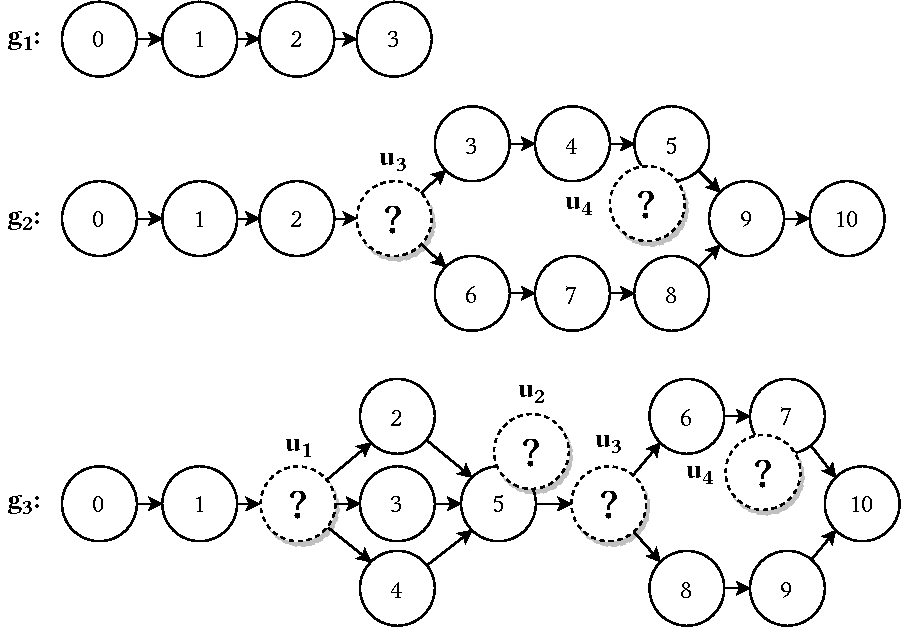
\includegraphics[width=\textwidth]{figures/chapter7/alltfgs.pdf}
    \caption{Simplified overview of all three \acfp*{TFG} of the running example with annotated primary and secondary uncertainties.}
    \label{fig:confidentialityanalysis:alltfgs}
\end{figure}

\autoref{fig:confidentialityanalysis:alltfgs} shows a simplified overview of all three \acp{TFG} of the running example.
We replace the vertices' names with numbers but keep the \emph{primary} uncertainty annotated to vertices, and \emph{secondary} uncertainty annotated to edges.
Note that we use a slightly different notation in this section to simplify the mathematical notation, e.g., $u_{1}$ refers to \U{1}.
This figure is based on \autoref{table:confidentialityanalysis:scenarios}, showing the scenarios of uncertainties \U{1} -- \U{4}, and \autoref{table:confidentialityanalysis:scenariostfgs}, showing the mapping of uncertainty sources to \acp{TFG}.
More detailed views of the second and third \acp{TFG} are shown in \autoref{fig:classification:dag} and \autoref{fig:confidentialityanalysis:dag}, respectively.
We also include the first \ac{TFG} representing the support contact request of the \emph{Customer}.
However, this \ac{TFG} is not affected by uncertainty, see \autoref{ch:runningexample}.

Let $G = \setted{g_{1}, g_{2}, \dots, g_{n}}$ where $n \geq 1$ be the nonempty finite set of all \acp{TFG} extracted from the architectural model, as introduced in \autoref{sec:confidentialityanalysis:framework}, and let $\abs{G}$ be its size.
In our running example, $G = \setted{g_{1},g_{2},g_{3}}$ and $\abs{G} = 3$.
Put simply, there are 3 extracted \acp{TFG}.
Let $U = \setted{u_{1}, u_{2}, \dots, u_{m}}$ where $m \geq 1$ be the nonempty finite set of all uncertainties, both \emph{primary} and \emph{secondary}, and let $ \abs{U}$ be the its size.
In our running example, $U = \setted{u_{1}, u_{2}, u_{3},u_{4}}$ and $\abs{U} = 4$.
Put simply, there are 4 uncertainties. 
We further split $U$ in $U_{P} \subseteq U$ to represent all \emph{primary} uncertainties and $U_{S} \subseteq U$ to represent all \emph{secondary} uncertainties in $U$.
This also means that $U = U_{P} \cup U_{S}$ and $U_{P} \cap U_{S} = \emptyset$.
In our running example, $U_{P} = \setted{u_{2}, u_{4}}$ and $U_{S} = \setted{u_{1}, u_{3}}$.
For each uncertainty source $u \in U $, let $ S_{u} = \setted{s_{u_{1}}, s_{u_{2}}, \dots, s_{u_{p}}}$ where $p \geq 1$ be the nonempty finite set of all uncertainty scenarios of $u$ and let $ \lvert S_{u} \rvert$ its size.
As discussed with \acp{NDFD} in \autoref{sec:confidentialityanalysis:typeagnostic}, $p \geq 1$ is trivially satisfied, as every uncertainty source has at least one default scenario.
In our running example, $ S_{u_{1}} = \{ s_{1}, s_{2}, s_{3} \}$ and $\abs{S_{u_{1}}} = 3$.
Put simply, the first uncertainty has three uncertainty scenarios, i.e., valid input, erroneous input, and malicious input, see \autoref{table:confidentialityanalysis:scenarios}.

Each uncertainty scenario brings variation into a \ac{TFG} and thus has to be analyzed separately.
This also applies to combinations of uncertainties, where every combination of all relevant scenarios of all relevant uncertainties has to be analyzed separately, i.e., the Cartesian product \cite{de_finetti_theory_2017}.
To minimize the analysis runtime and maximize its scalability, it is thus important to make a good estimation of what is \emph{relevant}.
Otherwise, the combination of scenarios can lead to the already discussed combinatorial explosion \cite{koziolek_automated_2011}.
We define $N$ as the number of \acp{TFG} that have to be analyzed in total.
In the following, we define three formulas to calculate this number, based on the underlying approach.
We define $N_{S}$ for the \emph{scenario-aware} analysis (\level{2}), $N_{G}$ for the \emph{graph-aware} analysis (\level{3}), and $N_{I}$ for the \emph{impact-aware} analysis (\level{4}).
Note that all three analysis approaches find the same confidentiality violations due to uncertainty, i.e., the accuracy is not affected.
However, the number of \acp{TFG} that have to be analyzed can differ.


The \emph{scenario-aware} analysis (\level{2}) does not consider \acp{TFG} but only combinations of scenarios.
Thus, for every possible scenario combination, every \ac{TFG} has to be analyzed which represents the least optimized approach.
We denote:

\begin{equation*}
N_{S} = \abs{G} \cdot \prod_{u \in U} \abs{S_{u}}
\end{equation*}

This is equivalent to generating all possible scenario combinations, applying them to all \acp{TFG}, and analyzing them, as introduced in \autoref{alg:confidentialityanalysis:scenarioaware}.
In our running example with 3 \acp{TFG} and 4 uncertainty sources, this means we have to analyze $N_{S} = \abs{G} \cdot \abs{S_{u_{1}}} \cdot \abs{S_{u_{2}}} \cdot \abs{S_{u_{3}}} \cdot \abs{S_{u_{4}}} = 3 \cdot 3 \cdot 4 \cdot 2 \cdot 2 = 144$ \acp{TFG}.
This is equivalent to analyzing all 3 \acp{TFG} in all 48 scenarios, as discussed in \autoref{sec:confidentialityanalysis:typespecifc}.


The \emph{graph-aware} analysis (\level{3}) does take \acp{TFG} into account and thus only has to consider combinations of scenarios in the same \ac{TFG}.
This is based on the finding that uncertainties in different flows, i.e., different \acp{TFG}, cannot affect each other, as discussed in \autoref{sec:impactanalysis:ufd}.
This highly reduces the amount of \acp{TFG} that have to be analyzed, especially in larger systems with many independent data flows.
To count the uncertainty sources $u \in U$ and its scenarios $S_{u}$ that impact a specific TFG $g \in G$, we define the \emph{impact function}:

\begin{equation*}
    f(g,u) = 
    \begin{cases}
        1,& \text{if there is no impact of } u \text{ on } g\\
        \abs{S_{u}},& \text{otherwise}
    \end{cases}
\end{equation*}

In our running example, $f(g_{2},u_{3}) = 2$, because the uncertainty $u_{3}$ in the \ac{TFG} $g_{2}$ has 2 scenarios.
To recall, the second \ac{TFG} represents the querying of items and Uncertainty \U{3} represents the deployment with the scenarios of being deployed on-premise or in the cloud.
$f(g_{1},u_{3}) = 1$, because the uncertainty $u_{3}$ has no effect on the first \ac{TFG}.
Put simply, this function yields the number of scenarios if the uncertainty is relevant for a \ac{TFG}; otherwise, it returns 1.
Using this function, we denote:

\begin{equation*}
    N_{G} = \sum_{g \in G} \prod_{u \in U} f(g,u)
\end{equation*}

This is equivalent to iterating over all \acp{TFG} and only generating the scenario combinations relevant for the current \ac{TFG}, as introduced in \autoref{alg:confidentialityanalysis:graphaware}.
In our example, the first \ac{TFG} has no uncertainty and $f$ always returns 1.
The second \ac{TFG} is only impacted by $u_{3}$ and $u_{4}$ while the third \ac{TFG} is impacted by all uncertainties.
In sum, this means: $N_{G} = (1 \cdot 1 \cdot 1 \cdot 1) + (1 \cdot 1 \cdot 2 \cdot 2) + (3 \cdot 4 \cdot 2 \cdot 2) = 1 + 4 + 48 = 53$ \acp{TFG}.
The number of \acp{TFG} that have to be analyzed by the \emph{graph-aware} approach is notably smaller compared to the \emph{scenario-aware} approach, i.e., $53 < 144$.
Although the third \ac{TFG} represents the worst case of combining all scenarios, the other \acp{TFG} are not affected.
Note that this formula only results in the same number as the \emph{scenario-aware} approach if all \acp{TFG} are affected by all uncertainties.
Trivially, this is the case if there is only one data flow within the system.
However, we assume that real-world software systems comprise more than a single data flow \cite{hahner_architecture-based_2023}.
Such a system would only provide a single functionality via a single interface with a single use case without any branching.
Thus, as \acp{TFG} are independent and an uncertainty impact can always assigned to a single \ac{TFG}, we find in general: 

\begin{equation*}
    N_{G} \leq N_{S}
\end{equation*}


The \emph{impact-aware} analysis (\level{4}) extends the \emph{graph-aware} analysis and additionally considers the transitive effect of the uncertainty scenarios.
By incrementally evaluating uncertainty scenarios, the impact of previous uncertainties in the same \ac{TFG} can be considered.
This enables us to analyze only those scenarios that are still relevant after other uncertainty scenarios have been applied in the direction of the data flow.
We consider uncertainty interactions between the \emph{secondary} uncertainties $U_{S}$ and \emph{primary} uncertainties $U_{P}$.
If an \emph{component} uncertainty, \emph{interface} uncertainty, or \emph{connector} uncertainty changes the edges of a \ac{TFG}, this affects all vertices---and all \emph{primary} uncertainties that affect such vertices---in the direction of the data flow, see \autoref{sec:confidentialityanalysis:typeagnostic}.

The easiest way to consider this in the calculation of relevant \acp{TFG} is to process all \acp{TFG} $g \in G$.
Similar to \autoref{alg:confidentialityanalysis:processvertex}, we replace all \emph{secondary} uncertainties $u \in U_{S}$ in all \acp{TFG} $g \in G$ with their scenarios.
Following the notion introduced in \autoref{sec:classification:dfd}, this means iterating over all $E_{u_{i}} \subseteq E$, i.e., all sets of alternative edges representing a \emph{secondary} uncertainty that form a subset of all edges of a \ac{DAG}.
For each edge $e \in E_{u_{i}}$, we create a copy of the current \ac{TFG} that contains the edge $e$ but none of the other edges in $E_{u_{i}}$.
The processing continues replacing \emph{secondary} uncertainty on the resulting \acp{TFG} until all \emph{secondary} uncertainties have been processed.
In sum, we define the function $p(G,U)$ that takes a set of \acp{TFG} $G$ and yields a set of \acp{TFG}, where all \emph{secondary} uncertainties in $U$ have been processed as described above.
As all uncertainties have at least one default scenario, we can say: $\abs{G} \leq \abs{p(G,U)}$.
Note that in contrast to \autoref{alg:confidentialityanalysis:processvertex}, we do not additionally process \emph{primary} uncertainty for the calculation as this uncertainty cannot alter edges in the \ac{TFG}.
Trivially, this means $\abs{p(G,U)} = \abs{p(G,U_{S})}$ and $\abs{G} = \abs{p(G,U_{P})}$.

In our running example, the second \ac{TFG} $g_{2}$ has one \emph{secondary} uncertainty $u_{3}$.
Applying this processing results in replacing the uncertainty $u_{3}$ with its affected edges, thereby creating 2 new \acp{TFG}, one with the edge $\flow{2}{3}$ and a second one with the edge $\flow{2}{6}$, see \autoref{fig:confidentialityanalysis:alltfgs}.
Thus, $\abs{p(\setted{g_{2}}, U)} = 2$.
The third \ac{TFG} $g_{3}$ has two \emph{secondary} uncertainties $u_{1}$ and $u_{3}$, with 3 and 2 scenarios, respectively.
Thus, $\abs{p(\setted{g_{3}}, U)} = 3 \cdot 2 = 6$.
We denote: 

\begin{equation*}
    N_{I} = \sum_{g \in p(G,U)} \prod_{u \in U_{P}} f(g,u)
\end{equation*}

This is equivalent to iterating over all vertices of all \acp{TFG} and taking the transitive impact of \emph{secondary} uncertainties into account, as introduced in \autoref{alg:confidentialityanalysis:impactaware}.
Note that we only calculate the product of \emph{primary} uncertainties, as we already considered the impact of the \emph{secondary} uncertainties in the processing $p(G,U)$.
In our running example, this does affect the calculation of the second and third \ac{TFG}.
As discussed previously, the second \ac{TFG} has one \emph{secondary} uncertainty.
After the processing of this uncertainty, only one of the two resulting \acp{TFG} is affected by the remaining \emph{primary} uncertainty.
This is the \ac{TFG} that represents the deployment in the cloud (\U{3}) that is affected by the provider's trustworthiness (\U{4}).
This effect becomes even bigger in the third \ac{TFG}.
Here, only half of the resulting \acp{TFG} represent a deployment in the cloud (\U{3}).
In sum, this means: $N_{I} = (1 \cdot 1) + ((1 \cdot 2) + (1 \cdot 1)) + ((4 \cdot 2) + (4 \cdot 2) + (4 \cdot 2) + (4 \cdot 1) + (4 \cdot 1) + (4 \cdot 1)) = 1 + (2 + 1) + (8 + 8 + 8 + 4 + 4 + 4) = 1 + 3 + 36 = 40$ \acp{TFG}.
We use parenthesis to highlight the \acp{TFG} after the processing.
This represents the minimum of scenarios and \acp{TFG} that have to be analyzed to identify all potential confidentiality violations, i.e., $40 < 53 < 144$.
As we replace every \emph{secondary} uncertainty in $U$ with additional graphs in $G$, we move them from the inner product to the outer sum in the formula.
Thus, we find in general: 

\begin{equation*}
    N_{I} \leq N_{G} \leq N_{S}
\end{equation*}





\section{Assumptions and Limitations}%
\label{sec:confidentialityanalysis:assumptions}

In this section, we discuss the assumptions and limitations of the different approaches of data flow analysis under uncertainty presented in this chapter.
This includes assumptions of single approaches and more general assumptions made in this chapter.
Note that we skip the limitations of the lower awareness levels \level{0} -- \level{3} compared to \emph{impact-aware} analysis (\level{4}) as we already comprehensively discussed their differences throughout this chapter.
The same applies to the comparison of \emph{type-specific} and \emph{type-agnostic} approaches.

\paragraph{Limitations of the data flow analysis framework}
Our approach for data flow analysis and the data flow analysis framework \cite{boltz_extensible_2024} are based on previous work in this field \cite{seifermann_architectural_2016,seifermann_identifying_2021,seifermann_unified_2021,seifermann_data-driven_2019,seifermann_detecting_2022,seifermann_architectural_2022,schneider_how_2024,schneider_microsecend_2023}.
Thus, we inherit some of the limitations.
First, the analysis operates on type-level, e.g., by analyzing usage scenarios and not individual users.
This restricts the expressiveness of analyzable confidentiality requirements \cite{seifermann_architectural_2022}.
Second, all four analysis approaches use the \ac{PCM} as an architectural model as previously discussed in \autoref{sec:impactanalysis:limitations}.
However, as the majority of the analysis is conducted on \acp{DFD}, the concepts should be generalizable.
First steps in this direction have already been taken \cite{boltz_extensible_2024}.
Third, the analysis does not respect state or time which limits the expressiveness but simplifies the analysis complexity \cite{seifermann_architectural_2022}.
Fourth, the labels used for confidentiality analysis represent discrete value sets, and there is no support for expressing continuous values other than mapping them to discrete values \cite{seifermann_architectural_2022}.
We refer to \textcite{seifermann_architectural_2022} for more detailed explanations of the reasoning behind these limitations.
Last, cycles within architectural models only have limited effects by only being traversed once.
However, there exist approaches for handling cycles in the construction of \acp{DAG} \cite{kramer_combining_1994,arp_analyzing_2024}.

\paragraph{Independence of data flow paths}
\textcite{seifermann_architectural_2022} discussed the assumption of independent data flow paths in data flow analysis.
Our data flow analysis framework presented in \autoref{sec:confidentialityanalysis:framework} follows this by assuming independence of extracted \acp{TFG} regarding the propagated labels that represent confidentiality-related characteristics of the software system.
Furthermore, we also assume that the impact of uncertainty in \acp{TFG} can be analyzed independently.
We argue that this assumption is reasonable.
The former can lead to an overestimation of confidentiality violations, which is acceptable.
The latter has been thoroughly discussed in \autoref{ch:classification} and \autoref{ch:impactanalysis}.

\paragraph{Modeling uncertainty scenarios}
The majority of approaches presented in this chapter are based on the assumption that modeling uncertainty scenarios is reasonable to express their effects on software systems, e.g., using design decision models \cite{koziolek_peropteryx_2011}, variation models \cite{walter_architecture-based_2023}, or uncertainty models \cite{hahner_model-based_2023}.
The description of uncertainty using scenarios has been discussed in the literature \cite{walker_defining_2003,mahdavi-hezavehi_classification_2017,armour_five_2000}, see \autoref{table:foundations:sources:locationlevel}.
\textcite{troya_uncertainty_2021} conducted a \acf{SLR} with 123 papers and support this assumption.
They found that \emph{design uncertainty} is usually expressed using uncertainty scenarios.

\paragraph{Analyzing unanticipated change}
We assume that the information required to model and analyze the software system under uncertainty is available to software architects.
A similar assumption has been made in the underlying approach for data flow analysis \cite{seifermann_architectural_2022} and also in earlier discussions of assumptions in \autoref{sec:classification:limitations} and \autoref{sec:impactanalysis:limitations}.
Similarly, we cannot express or analyze not yet identified uncertainty sources.
Nevertheless, we provide software architects with means to express uncertainty models within the architectural models and refine this model once more knowledge is gained.
The connection of data flow analysis to our catalog presented in \autoref{sec:classification:identification} further addresses this limitation. 

\paragraph{Multiple data flows and secondary uncertainty}
In this chapter, we present multiple approaches for data flow analysis under uncertainty.
The increased scalability of the \emph{graph-aware} analysis (\level{3}) and \emph{impact-aware} analysis (\level{4}) is based on two assumptions on the modeled software system.
First, we assume that real-world software systems comprise more than a single data flow path.
As discussed previously, such a system would only provide a single functionality via a single interface with a single use case without any branching.
Second, we assume the existence of \emph{secondary} uncertainty within the software system.
We argue that this is reasonable as three of the five uncertainty types introduced in \autoref{table:classification:classification:architecturalelementtype} represent \emph{secondary} uncertainty.
If this assumption does not hold, the latter analysis approaches are still applicable.
However, their benefits regarding the analysis complexity are decreased.

\paragraph{Limited support for uncertainty interactions}
Based on our findings on uncertainty propagation and \acp{UFD} presented in \autoref{sec:impactanalysis:ufd}, the \emph{impact-aware} analysis (\level{4}) supports simple uncertainty interactions.
However, this support is limited to the impact of \emph{secondary} uncertainty on \emph{primary} uncertainty.
Put simply, altering the edges of a \ac{DAG} can affect the flow of data to vertices and thus can also affect the impact of \emph{primary} uncertainty on these vertices.
Further uncertainty interactions can happen, e.g., between two \emph{primary} uncertainties where one uncertainty voids the impact of another uncertainty.
This limitation is similar to the overestimation of the uncertainty impact discussed in \autoref{sec:impactanalysis:limitations}.
Addressing this requires a higher expressiveness in the modeling and analysis as more fine-grained interactions between uncertainty and confidentiality have to be considered.

\paragraph{Mitigation of uncertainty}
We consider the automated mitigation of uncertainty as out of the scope of this thesis.
This includes the automated repair of uncertainty-afflicted software systems due to confidentiality violations.
Additionally, we only focus on finding all potential confidentiality violations due to uncertainty.
Analysis approaches that aim for fast feedback for software architects by returning partial results could thus further increase the analysis scalability.
We emphasize that advanced approaches to analysis, mitigation, and repair are expedient and that our analysis approaches can provide a comprehensive foundation for such endeavors. 

\paragraph{Uncertainty in confidentiality requirements}
We do not consider any uncertainty within confidentiality requirements that can occur, e.g., due to the relation to legal assessment \cite{boltz_model-based_2022}.
This would require means to express uncertainty-related variation not only as part of the software system but also in the specification of data flow constraints.
This could be achieved, e.g., by extending existing \acfp{DSL} \cite{hahner_modeling_2021,boltz_extensible_2024}.
Similar to the previous limitation, we emphasize the importance of this research but consider it to be out of scope for this thesis.





\section{Summary and Outlook}%
\label{sec:confidentialityanalysis:summary}

In this chapter, we presented multiple approaches to uncertainty-aware data flow analysis to identify potential confidentiality violations due to uncertainty.
This represents our third Contribution \C{3} and provides an answer to \RQ{3}.

First, we discussed the foundations required to define uncertainty-aware data flow analyses, as described with Problem \PR{3}{1}.
We presented an extensible framework for data flow analysis \cite{boltz_extensible_2024} that enables both black-box and white-box extensions \cite{taghavi_survey_2023,heinrich_composing_2021} of confidentiality analysis.
Here, we also introduced the concepts of \acp{TFG} and label propagation.
Afterward, we discussed which information is available in data flow analysis under uncertainty and how this information can be used.
To that end, we specified five levels (\level{0} -- \level{4}) of uncertainty awareness: The lack of uncertainty-awareness (\level{0}), naive approaches (\level{1}), scenarios-awareness (\level{2}), graph-awareness (\level{3}), and impact-awareness (\level{4}).
Uncertainty-aware data flow analyses that fall into one of these categories can be further categorized into type-specific and type-agnostic approaches.

Building on these foundations, we presented two \emph{type-specific} approaches to data flow analysis under uncertainty.
This addresses Problem \PR{3}{2}.
First, we introduced a \emph{scenario-aware} analysis (\level{2}) of structural uncertainty.
By combining the design space exploration approach PerOpteryx \cite{koziolek_peropteryx_2011,koziolek_automated_2011} with data flow analysis, we can identify confidentiality violations in software architecture candidates.
This enables the analysis of structural uncertainty, e.g., due to an uncertain deployment of a component.
Second, we introduced a \emph{graph-aware} analysis (\level{3}) of environmental uncertainty.
Here, we used fuzzy inference in the form of \acp{FIS} to express natural factors in the environment of a software system that can affect access control decisions and, thus, confidentiality.
We found that both analysis approaches share the representation of uncertainty sources as one or multiple scenarios.

Last, we moved towards \emph{type-agnostic} approaches for uncertainty-aware data flow analysis to address Problem \PR{3}{3}.
First, we presented a \emph{graph-aware} analysis (\level{3}) that uses variation modeling \cite{mehl_palladio_2022,walter_architecture-based_2023} to trace confidentiality violations back to uncertainty sources.
Being \emph{type-agnostic}, this approach supports all five uncertainty types introduced in \autoref{sec:classification:classification}.
To also support simple forms of uncertainty interactions, we introduced an \emph{impact-aware} analysis (\level{4}) thereafter.
We closed the gap between the uncertainty classification and confidentiality analysis by providing a meta model for modeling uncertainty sources and scenarios.
The analysis incrementally considers the impact of uncertainty within the data flow and thus can respect relations between multiple uncertainties.
We also introduced \abunai, our \ac{PCM}-based tooling for uncertainty \emph{impact-aware} data flow analysis (\level{4}).
We concluded this discussion by comparing the complexity of the presented analyses.

\RQ{3} asked about the analysis of confidentiality requirements using architecture-based data flow analysis that considers uncertainty within the architectural model and thus becomes uncertainty-aware.
To answer this question, we provided a discussion of available information, resulting awareness levels of data flow analyses and analysis complexity and scalability.
Furthermore, we presented four analysis approaches that differ in supported uncertainty types, awareness levels (\level{2} -- \level{4}) and type specificity.
As pointed out earlier, there is no single best answer to the question of architecture-based confidentiality analysis under uncertainty.
Thus, our approach to this chapter was to provide a comprehensive discussion of multiple solutions and their trade-offs.

There are multiple benefits of the variety of analysis approaches presented in this chapter with Contribution \C{3}.
In general, considering uncertainty within an analysis enables more precise and more comprehensive analysis results of a model and its context \cite{weyns_towards_2023,weyns_introduction_2020,perez-palacin_dealing_2014}.
Here, all four approaches can be used standalone, thus providing means to model and analyze different types of uncertainty.
An automated analysis like \abunai supports architects by reducing the manual effort, especially in large models with many independent data flows and many uncertainty sources \cite{hahner_model-based_2023}.
Furthermore, describing uncertainties as a first-class entity and part of the architectural model helps in the documentation \cite{hahner_classification_2023}.
Although we focused on confidentiality, our \emph{impact-aware} analysis is also an approach to consider uncertainty interactions within the architecture-based analysis.
Together with our finding on \acp{UFD}, this can be used to further address the \ac{UIP}.
Last, our data flow analysis framework can be used to define new analysis approaches, even without the need to focus on uncertainty \cite{boltz_extensible_2024}.

The contribution provided in this chapter was based on the findings from \readingpath{ch:classification} and \readingpath{ch:impactanalysis}.
We used many of the concepts introduced in these earlier chapters, e.g., the five uncertainty types, or the representation of uncertainty in \acp{DAG} as \emph{primary} and \emph{secondary} uncertainty.
Also, the foundations for uncertainty propagation and interaction were laid in these chapters.
The confidentiality analysis with respect to uncertainty represents the last step of the procedure presented in \readingpath{ch:overview}.
The next chapters show an overview of \readingpath{ch:evaluationscenarios} and then present the \readingpath{ch:evaluation} of all contributions.





\section{In Simpler Words}%
\label{sec:confidentialityanalysis:simple}

Confidentiality describes the property that information is not disclosed to persons or organizations that should not see this information.
Put simply, if you tell me a secret, I should keep it secret---treating it confidential.
The same applies to software systems and the data that is handled by these systems.
If you enter your personal data, such as your name, date of birth, or credit card details, into an online shop, you assume that you can trust the shop and that your information is treated confidentially.

Architecture-based confidentiality analyses have been proposed to analyze the confidentiality of a software system at a high abstraction or early in the system design.
These analyses use a model of the system and confidentiality requirements as input and identify confidentiality violations.
For example, if a law requires your confidential data to be stored on a server in the same country, but the system sends it across a border, this would represent a confidentiality violation.
To identify such violations, we analyze all data flows in a software architecture---this is called \emph{data flow analysis}.

In the previous chapters, we already introduced the notion of uncertainty and also discussed that uncertainty can negatively impact a software system's confidentiality.
For instance, if we do not know whether your data is actually sent to a server in another country, we cannot state that it is confidential.
To identify confidentiality violations under uncertainty, we define several uncertainty-aware data flow analyses.
In this chapter, we present four different analysis approaches that use different algorithms to see how uncertainty impacts confidentiality.
Some of these approaches are tailored to one uncertainty type, such as uncertainty in a software system's environment.
Other approaches support all uncertainty types that have been identified in \autoref{ch:classification}.
We call the former \emph{type-specific} analyses and the latter \emph{type-agnostic} analyses.
Additionally, we investigate the information used by the analysis and define five levels of uncertainty awareness.

Although the four presented approaches differ regarding the level of uncertainty awareness, they share the representation of uncertainty in the form of scenarios.
A scenario represents one possible outcome of uncertainty, e.g., whether your data flows across a country border.
The uncertainty-aware analysis considers these scenarios in analyzing confidentiality and returns only those scenarios that violate confidentiality.
This helps software architects to better assess whether or not an uncertainty is critical and should be mitigated.
Some approaches find such critical scenarios by checking all possible variations of the software architecture.
Other approaches use the available information in a more clever way and can exclude irrelevant scenarios early in the analysis.

The most advanced approaches center their analysis algorithm around uncertainty.
They treat uncertainty as a so-called first-class entity or first-class concern.
This means that uncertainty is of central importance and as important as every other element of the software architecture.
We find that considering uncertainty in this way helps to provide more and better information to the software architects.
Additionally, the analysis scales better for large software systems from the real world.
We also implemented such an analysis and provided it together with this thesis.
This represents the final contribution of this thesis and also concludes the procedure that has been introduced in \autoref{ch:overview}.


\part{Validation}
\chapter{Evaluation Scenarios}%
\label{ch:evaluationscenarios}%


In this chapter, we present the scenarios used in the evaluation of this thesis.
We do not perform \emph{case studies} as we do not study the use of our contributions in a real-life environment, e.g., by watching software architects or security experts \cite{wohlin_case_2021}.
We use the term \emph{evaluation scenario} instead as we only investigate the intended use of our contributions based on real-world systems, similar to related work \cite{runeson_guidelines_2009,walter_context-based_2023}.
Nevertheless, using case study systems in the evaluation of contributions in the software architecture community is common \cite{walter_context-based_2023,seifermann_architectural_2022,busch_architecture-based_2020}.
\textcite{konersmann_evaluation_2022} conducted a \acf{SLR} with 153 papers and found that using case study systems represents the most common evaluation method in recent software architecture research.

In this thesis, every \emph{evaluation scenario} is based on or related to a real software system that has been specified by others.
Thus, we start each scenario with a description of its source, where it is used, and how the architectural models have been created.
Afterward, we describe the software system of each scenario, which includes the software architecture and its intended use.
Every scenario handles confidential data and thus has confidentiality requirements that can be specified as data flow constraints.
Last, a real-world software system is subject to uncertainty.
We discuss uncertainty sources and their potential impact on confidentiality based on existing collections \cite{hahner_classification_2023,ramirez_taxonomy_2012,hahner_arcn_2024}.

This chapter introduces six evaluation scenarios.
The first three, namely the \emph{TravelPlanner}, \emph{DistanceTracker}, and \emph{OnlineShop} scenarios have been used in the evaluation of related approaches \cite{walter_context-based_2023,seifermann_architectural_2022,seifermann_detecting_2022,seifermann_data-driven_2019,kunz_efficient_2018,weimann_automated_2017,walter_architectural_2022-1,walter_architecture-based_2023,walter_tool-based_2023,kramer_model-driven_2017}.
The second three, namely the \emph{CoronaWarnApp}, \emph{MobilityAsAService}, and \emph{JPlag}, represent software systems from academia \cite{leinweber_leveraging_2023,prechelt_finding_2002,saglam_automated_2024,saglam_detecting_2024,saglam_obfuscation-resilient_2024,saglam_token-based_2022} and industry \cite{robert_koch_institute_open-source_2020,enaya_case_2024}.
In the following, we give an overview of the evaluation scenarios and then introduce them in more detail.
See the data set \cite{dataset} for all data flow constraints and \acf{PCM} instances.

\ownpublications{
\fancycite{hahner_architectural_2021}, 
\fancycite{boltz_handling_2022},
\fancycite{walter_architectural_2022},
\fancycite{hahner_model-based_2023},\linebreak
\fancycite{hahner_classification_2023},
\fancycite{hahner_architecture-based_2023},
\fancycite{boltz_extensible_2024},\linebreak
\fancycite{hahner_arcn_2024}
}





\section{Overview}%
\label{sec:evaluationscenarios:overview}

\begin{table}
    \begin{tabularx}{\linewidth}{lllX}
        \toprule
        Name & Domain & Origin & Used in \\
        \midrule
        TravelPlanner & Mobility & \cite{katkalov_model-driven_2013,katkalov_modellgetriebener_2017} & \cite{walter_context-based_2023,seifermann_architectural_2022,seifermann_detecting_2022,seifermann_data-driven_2019,walter_architectural_2022-1,walter_architecture-based_2023,walter_tool-based_2023,kramer_model-driven_2017,hahner_model-based_2023,hahner_modeling_2021,walter_architectural_2022,boltz_handling_2022,schwickerath_tool-supported_2023} \\
        DistanceTracker & Health / Sports & \cite{katkalov_modellgetriebener_2017} & \cite{seifermann_architectural_2022,seifermann_detecting_2022,seifermann_data-driven_2019,hahner_model-based_2023,hahner_modeling_2021,walter_architectural_2022,boltz_handling_2022}  \\
        OnlineShop & E-Commerce & \cite{seifermann_data-driven_2019,rausch_common_2008} & \cite{walter_architectural_2022,kunz_efficient_2018,weimann_automated_2017,hahner_domain-specific_2020,hahner_model-based_2023,boltz_extensible_2024,hahner_architectural_2021,hahner_arcn_2024,hahner_classification_2023,hahner_architecture-based_2023} \\
        CoronaWarnApp & Health & \cite{robert_koch_institute_open-source_2020,enaya_case_2024} & \cite{hahner_classification_2023,hahner_architecture-based_2023,hahner_architecture-based_2024} \\
        MobilityAsAService & Mobility & \cite{leinweber_leveraging_2023} & - \\
        JPlag & Plagiarism Detection & \cite{prechelt_finding_2002,saglam_obfuscation-resilient_2024} & - \\
        \bottomrule
    \end{tabularx}
    \caption{Overview of all evaluation scenarios, their domain, their origin, and their usage.}%
    \label{table:evaluationscenarios:overview}
\end{table}

For the evaluation of this thesis, we use software systems and scenarios of different size and from different domains.
\autoref{table:evaluationscenarios:overview} shows an overview of the six evaluation scenarios, their origin, and other evaluations where they have already been used.
To encounter threats to external validity and to increase generalizability, we use scenarios from different domains, e.g., from the mobility or health domain.
All evaluation scenarios originate from other work.
The majority have been used in the evaluation of other publications.
Only the last two scenarios, \emph{MobilityAsAService} a service and \emph{JPlag} are new.
However, they represent well-evaluated systems with high demands on the systems' confidentiality and are thus suitable as evaluation scenarios for this thesis.

\begin{table}
    \begin{tabularx}{\linewidth}{lZZZZZZ}
        \toprule
        Name & \rot{\# Component} & \rot{\# \ac{SEFF}} & \rot{\# \ac{TFG}} & \rot{\# Vertex} & \rot{\# Uncertainty} & \rot{\# Violation} \\
        \midrule
        TravelPlanner & 7 & 9 & 2 & 42 & 1 & 1 \\
        DistanceTracker & 8 & 10 & 1 & 29 & 1 & 1 \\
        OnlineShop & 2 & 6 & 3 & 44 & 4 & 24 \\
        CoronaWarnApp & 21 & 58 & 14 & 687 & 9 & 163 \\
        MobilityAsAService & 18 & 49 & 8 & 200 & 5 & 6 \\
        JPlag & 3 & 5 & 3 & 65 & 4 & 26 \\
        \bottomrule
    \end{tabularx}
    \caption{Size metrics, uncertainty sources, and confidentiality violations of all evaluation scenarios.}%
    \label{table:evaluationscenarios:size}
\end{table}

For the contributions of this thesis (\C{1}, \C{2}, and \C{3}), a central property of a software system is the form and size of the system's \acf{DFD} and the scenario's uncertainty sources, as discussed in \autoref{sec:classification:dfd} and \autoref{sec:confidentialityanalysis:typeagnostic}.
\autoref{table:evaluationscenarios:size} lists all relevant size-related metrics of the six evaluation scenarios.
This includes the number of the components and \acfp{SEFF} of the \ac{PCM} instance of each scenario, as these numbers impact the number of \ac{DFD} nodes.
We also show the number of \acfp{TFG} and their vertices, because these sizes are relevant both for the uncertainty impact analysis (\C{2}) and for the different approaches to uncertainty-aware data flow analysis (\C{3}).
Last, we show the number of uncertainty sources in the evaluation scenarios and the number of potential confidentiality violations due to these uncertainties.

The scenarios show different sizes and numbers of uncertainties and violations. The \emph{TravelPlanner} and the \emph{DistanceTracker} represent smaller scenarios with one uncertainty source each, and 7 and 8 components, respectively.
Still, their \acp{TFG} have a total of 42 and 29 vertices, which highlights again the need for automated analysis approaches and tool support, discussed in \autoref{sec:overview:toolsupport}.
\emph{MobilityAsAService} and \emph{CoronaWarnApp} are the largest evaluation scenarios.
They contain 5 and 9 uncertainty sources and a total of 200 and 687 \ac{TFG} vertices that represent \ac{DFD} nodes.





\section{TravelPlanner}%
\label{sec:evaluationscenarios:travelplanner}

\begin{figure}
    \centering
    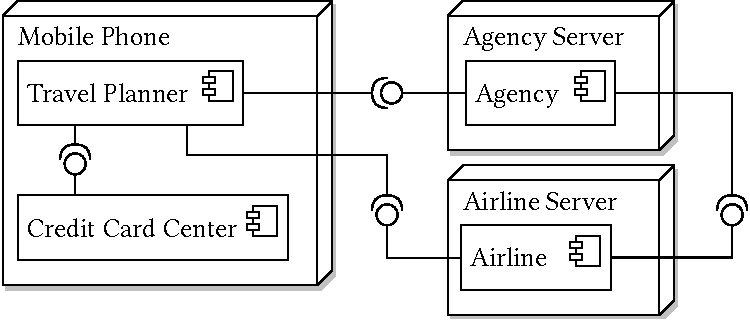
\includegraphics[width=0.7\textwidth]{figures/chapter8/scenario1_travelplanner.pdf}
    \caption{Simplified component and deployment diagram of the TravelPlanner evaluation scenario.}
    \label{fig:evaluationscenarios:travelplanner}
\end{figure}

\paragraph{Source}
The \emph{TravelPlanner} evaluation scenario originates from the iFlow project by \textcite{katkalov_modellgetriebener_2017}.
It originally has been used in the evaluation of information flow analysis \cite{katkalov_model-driven_2013}.
A comprehensive description of the software architecture and a Java-based implementation are available \cite{katkalov_modeling_2013}.
The \ac{PCM} model used in this evaluation scenario stems from related work \cite{seifermann_architectural_2022,walter_context-based_2023} and has been used in many case study-based validations \cite{seifermann_detecting_2022,seifermann_data-driven_2019,walter_architectural_2022-1,walter_architecture-based_2023,walter_tool-based_2023,kramer_model-driven_2017,hahner_model-based_2023,hahner_modeling_2021,walter_architectural_2022,boltz_handling_2022,schwickerath_tool-supported_2023}.

\paragraph{Description}
\autoref{fig:evaluationscenarios:travelplanner} shows a simplified diagram of the software architecture.
Here---and also in all following figures of this chapter---we show simplified diagrams to give an overview and to increase clarity.
As shown in \autoref{table:evaluationscenarios:size}, the \ac{PCM} model consists of more components than illustrated.
We do also not depict uncertainty sources in this diagram.
We refer to the data set \cite{dataset} for the complete architectural model, which includes data flow constraints and uncertainty models.
The corresponding \ac{PCM} model consists of 7 components with 9 \acp{SEFF} and maps to 2 \acp{TFG} with 42 vertices.

This evaluation scenario comprises three central entities: A customer, a travel agency, and an airline.
The customer uses the \emph{Travel Planner} app to search for flights.
This app communicates with a travel \emph{Agency} that queries flights from multiple \emph{Airlines}.
The aggregated results are returned to the customer.
Afterward, the customer selects and books a flight using a credit card.
The software architecture comprises three deployment locations that match the three entities.
The customer operates the \emph{Mobile Phone}, where the \emph{Travel Planner} app and the \emph{Credit Card Center} app is located.
Both the \emph{Agency} and the \emph{Airline} operate their own servers and provide interfaces to the other components.

\paragraph{Confidentiality requirements}
In this evaluation scenario, we consider two different data types.
On the one hand, the flight data represents public information without any data flow constraints.
On the other hand, credit card data represents highly sensitive information with strict confidentiality requirements.
This information is managed by the \emph{Credit Card Center} and shall only leave the \emph{Mobile Phone} in the booking process upon explicit approval by the customer.
Additionally, the credit card data shall only flow directly to the \emph{Airline} in the booking process---it shall never flow to the \emph{Agency}.

\paragraph{Uncertainty sources}
We use this evaluation scenario as a minimal scenario for \emph{primary} uncertainty.
We add the \emph{Behavior} uncertainty that credit card data can be used with or without user consent \cite{hahner_model-based_2023}.
Here, passing the data to the \emph{Airline} servers without consent represents a violation of the aforementioned confidentiality requirements.





\section{DistanceTracker}%
\label{sec:evaluationscenarios:distancetracker}

\begin{figure}
    \centering
    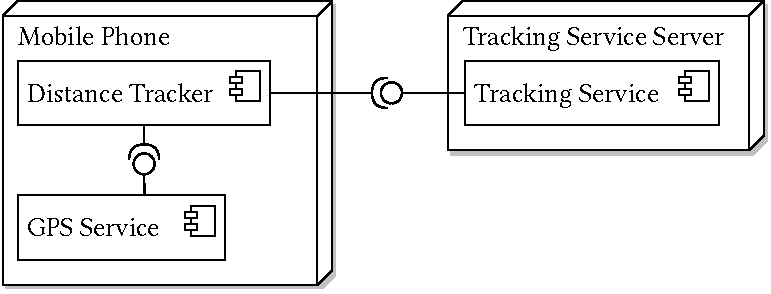
\includegraphics[width=0.7\textwidth]{figures/chapter8/scenario2_distancetracker.pdf}
    \caption{Simplified component and deployment diagram of the DistanceTracker evaluation scenario.}
    \label{fig:evaluationscenarios:distancetracker}
\end{figure}

\paragraph{Source}
The \emph{DistanceTracker} evaluation scenario also originates from the iFlow project by \textcite{katkalov_modellgetriebener_2017}.
Similarly to the \emph{TravelPlanner} scenario described above, it has been used in many case study-based validations \cite{seifermann_architectural_2022,seifermann_detecting_2022,seifermann_data-driven_2019,hahner_model-based_2023,hahner_modeling_2021,walter_architectural_2022,boltz_handling_2022}.

\paragraph{Description}
\autoref{fig:evaluationscenarios:distancetracker} shows a simplified diagram of the software architecture.
As discussed above, we simplify the system structure and do not depict uncertainty sources to increase clarity and refer to the data set \cite{dataset}.
The corresponding \ac{PCM} model consists of 8 components with 10 \acp{SEFF} and maps to 1 \ac{TFG} with 29 vertices.

The evaluation scenario comprises three central entities: The user, the \emph{Distance Tracker} app, and the online \emph{Tracking Service}.
The user shares the GPS location with the tracking app that periodically tracks the current location and calculates the distance run.
This distance is transmitted to the \emph{Tracking Service}.
The software architecture comprises two deployment locations.
The user operates the \emph{Mobile Phone} that hosts the \emph{Distance Tracker} app and a \emph{GPS service}.
The \emph{Tracking Service} is deployed on a separate server.

\paragraph{Confidentiality requirements}
The confidentiality requirement of this evaluation scenario considers the confidentiality of GPS data, i.e., precise information about the user's current location.
This information is only allowed to be used locally on the \emph{Mobile Phone}.
Only in aggregated form, e.g., as calculated distance, this information is allowed to be passed to the \emph{Tracking Service}.
Thus, there shall be no flow of explicit GPS locations from the \emph{Mobile Phone} to any other location.

\paragraph{Uncertainty sources}
We use this evaluation scenario as a minimal scenario for \emph{secondary} uncertainty.
We add the \emph{Connector} uncertainty that GPS data can be processed on the \emph{Tracking Service Server} \cite{hahner_model-based_2023} for additional statistics and a persisted history of runs.
Passing the GPS data to the \emph{Tracking Service} for this purpose is a confidentiality violation.





\section{OnlineShop}%
\label{sec:evaluationscenarios:onlineshop}

\begin{figure}
    \centering
    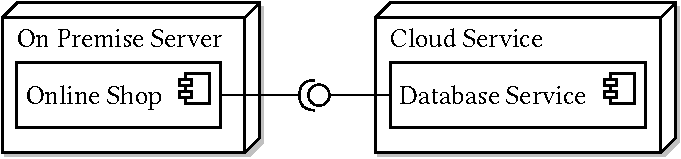
\includegraphics[width=0.65\textwidth]{figures/chapter8/scenario3_onlineshop.pdf}
    \caption{Simplified component and deployment diagram of the OnlineShop evaluation scenario.}
    \label{fig:evaluationscenarios:onlineshop}
\end{figure}

\paragraph{Source} 
The \emph{OnlineShop} evaluation scenario is based on CoCoME \cite{rausch_common_2008} and has been adapted for architecture-based confidentiality analysis \cite{seifermann_data-driven_2019}.
It has also been used in case study-based validations \cite{walter_architectural_2022,kunz_efficient_2018,weimann_automated_2017,hahner_domain-specific_2020,hahner_model-based_2023,boltz_extensible_2024,hahner_architectural_2021,hahner_arcn_2024,hahner_classification_2023,hahner_architecture-based_2023}.
We refer to this evaluation scenario throughout this thesis as the running example\footnote{Although using an evaluation scenario as the running example represents a threat to validity, we argue that this threat is weakened by using other evaluation scenarios in addition. Furthermore, the increased understanding arising from such thorough investigation can benefit the evaluation.}, see \autoref{ch:runningexample}.

\paragraph{Description}
\autoref{fig:evaluationscenarios:onlineshop} shows a simplified diagram of the software architecture.
A comprehensive diagram of the software system is shown in \autoref{fig:runningexample:architecture}, and the architectural model is part of the data set \cite{dataset}. 
The corresponding \ac{PCM} model consists of 2 components with 6 \acp{SEFF} and maps to 3 \acp{TFG} with 44 vertices.

The evaluation scenario comprises three central entities: The customer, the \emph{Online Shop}, and the shop's \emph{Database Service}.
We consider three usage scenarios: The user can query available items, purchase items, and request a support contact.
The former two scenarios include calls of the \emph{Online Shop} to the \emph{Database Service}, the latter only yields static information.
The software architecture comprises two deployment locations.
The \emph{Online Shop} is deployed \emph{On Premise} while the \emph{Database Service} is deployed to a \emph{Cloud Service}.
We refer to \autoref{ch:runningexample} for a more detailed description of the software system.

\paragraph{Confidentiality requirements}
In this evaluation scenario, we consider two different data types.
The public information of the online shop, like available items, and the user's private purchase details.
While the former is publicly available and not sensitive, the latter is highly sensitive, comparable to the credit card details of the \emph{TravelPlanner} evaluation scenario.
The user input in the purchase process shall be validated and encrypted before flowing into the database.
Additionally, depending on the deployment location and the trustworthiness of the resource provider, confidentiality can be threatened.
We provide more details on the confidentiality requirements in \autoref{ch:runningexample}.

\paragraph{Uncertainty sources}
We define four uncertainty sources in this evaluation scenario, as described in \autoref{sec:runningexample:uncertainty}.
Uncertainty \U{1} affects the user input that can be valid, erroneous, or malicious.
Uncertainty \U{2} affects the data processing in the \emph{Online Shop} component that can validate or encrypt the data.
Uncertainty \U{3} affects the deployment of the \emph{Database Service} component that can be on-premise or in the cloud. 
Uncertainty \U{4} affects the trustworthiness of the provider of the \emph{Cloud Service} that can be trustworthy or suspicious.
All uncertainty sources and their scenarios are shown in \autoref{table:confidentialityanalysis:scenarios}.





\section{CoronaWarnApp}%
\label{sec:evaluationscenarios:coronawarnapp}

\begin{figure}
    \centering
    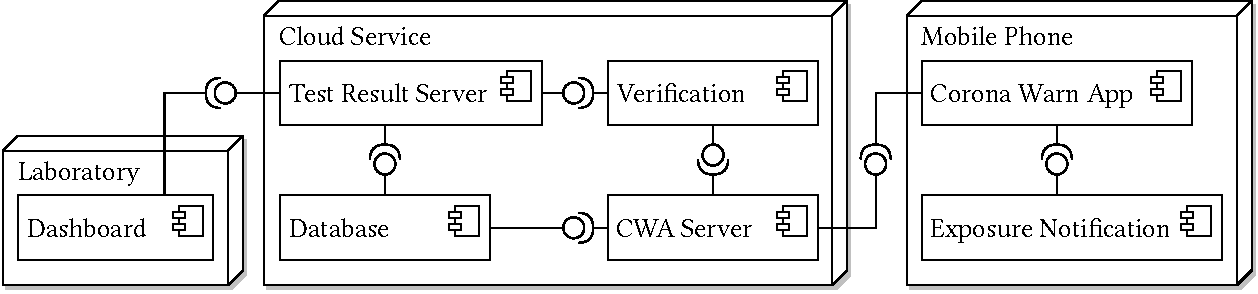
\includegraphics[width=\textwidth]{figures/chapter8/scenario4_coronawarnapp.pdf}
    \caption{Simplified component and deployment diagram of the CoronaWarnApp evaluation scenario.}
    \label{fig:evaluationscenarios:coronawarnapp}
\end{figure}

\paragraph{Source}
The \emph{CoronaWarnApp} evaluation scenario is based on the German Contact Tracing App of the same name \cite{robert_koch_institute_open-source_2020}.
During the COVID-19 pandemic, this app was used to warn users who may have come into contact with people who had tested positive on COVID-19.
The app was developed by SAP and Deutsche Telekom \cite{enaya_case_2024}, published by the Robert Koch Institute, and downloaded more than 20 million times \cite{robert_koch_institute_open-source_2020}.
All source code and documentation are available open-source on GitHub \cite{sap_corona-warn-app_2023}, including a detailed description of the software architecture.
We used the publicly available information to create a \ac{PCM} model that was already used in multiple validations \cite{hahner_classification_2023,hahner_architecture-based_2023,hahner_architecture-based_2024}.

\paragraph{Description}
\autoref{fig:evaluationscenarios:coronawarnapp} shows a simplified diagram of the software architecture.
Due to the size of the evaluation scenario, we leave out many details in this diagram, e.g., the collection of statistics, or the international exchange of positive test results.
The \ac{PCM} component repository model is shown in \autoref{sec:appendix:cwa}.
The corresponding \ac{PCM} model consists of 21 components with 58 \acp{SEFF} and maps to 14 \acp{TFG} with 687 vertices.

The evaluation scenario comprises five central entities.
The user of the app, the server infrastructure, laboratories, support hotlines, and international partners.
Users can voluntarily enter if they are infected to warn others and they also get warned in the case of a potential contact.
The warning mechanism uses keys that are exchanged between mobile phones via Bluetooth \cite{sap_corona-warn-app_2023}.
If users are tested, they can enter the test via a code or with the help of the support hotline.
The laboratories add the test results, and the server infrastructure manages both.
Additionally, the keys of positive tested users can be shared with international partner servers in the EU and Switzerland.
The components of the server infrastructure, e.g., the \emph{Verification}, or the \emph{Test Result Server}, are deployed to the \emph{Cloud Service} of the Open Telekom Cloud.
Laboratories operate their own \emph{Dashboards} and laboratory information systems that connect to the server infrastructure.
Users have the \emph{Corona Warn App} installed on their phones that communicate with the \emph{Exposure Notification} framework.
This framework manages the key exchange and comparison.

\paragraph{Confidentiality requirements}
The Corona Warn App manages sensitive information related to health data and location data.
Contact tracing apps are challenged with many risks, e.g., regarding de-anonymization or profiling \cite{baumgartner_mind_2020}.
We express multiple confidentiality requirements as data flow constraints \cite{hahner_modeling_2021,boltz_extensible_2024}.
First, users should not be able to directly access the exchanged keys but only be warned if an exchanged key matches a key of a person who tested positive.
Additionally, all keys and other credentials are considered to be sensitive information.
Here, the \emph{Verification} component plays a central role in the validation.
The Corona Warn App collects statistical data that shall only be shared in aggregated form.
Last, we reuse the already discussed requirements regarding secure storage, information leaks, and logging.
The full list of requirements is in data set \cite{dataset}.

\paragraph{Uncertainty sources}
Due to the size of this evaluation scenario, we model 4 sub-scenarios with 2 to 3 uncertainty sources each, which adds up to a total of 9 uncertainty sources.
In this first sub-scenario, we consider the processing of data and the interception of the communication regarding a central component in the \emph{Cloud Service}.
The second sub-scenario focuses on deployment and secure storage of test results using the \emph{Test Result Server}.
The third sub-scenario evolves around logging and validation in the \emph{Verification} component.
In the fourth sub-scenario, we focus on critical points within the system with a potentially wide impact, e.g., the \emph{Database} and the \emph{Exposure Notification} framework.
All details about the uncertainty sources and scenarios can be found in the data set \cite{dataset}.





\section{MobilityAsAService}%
\label{sec:evaluationscenarios:mobilityasaservice}

\begin{figure}
    \centering
    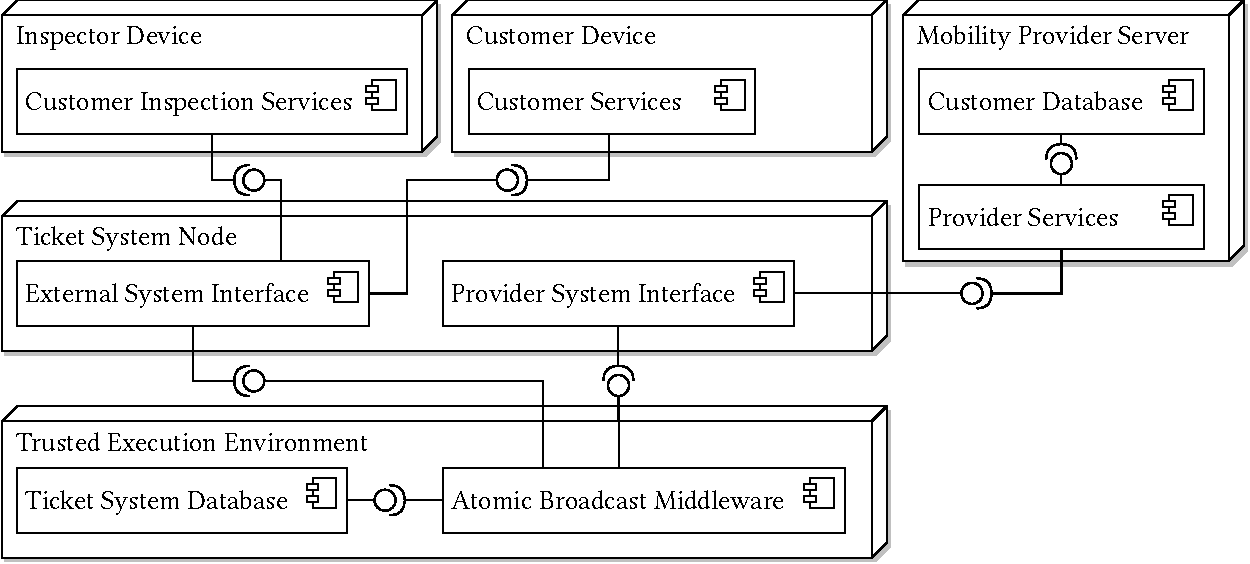
\includegraphics[width=\textwidth]{figures/chapter8/scenario5_mobilityasaservice.pdf}
    \caption{Simplified component and deployment diagram of the MobilityAsAService evaluation scenario.}
    \label{fig:evaluationscenarios:mobilityasaservice}
\end{figure}

\paragraph{Source}
The \emph{MobilityAsAService} evaluation scenario is based on a concept for a distributed ticketing system of the same name \cite{leinweber_leveraging_2023}.
It uses \acf{DLT} with \acfp{TEE} to define a secure system with distributed governance that is scalable while ensuring confidentiality.
We used the available documentation to create a \ac{PCM} model that approximates the proposed concept.

\paragraph{Description}
\autoref{fig:evaluationscenarios:mobilityasaservice} shows a simplified diagram of the software architecture.
As we use the \ac{ADL} \ac{PCM} to model the scenario, we can only approximate the actual behavior of a \ac{DLT}, or a \ac{TEE}.
Additionally, we only model one mobility provider, while the underlying concept allows for many operators with decentralized governance. 
The corresponding \ac{PCM} model consists of 18 components with 49 \acp{SEFF} and maps to 8 \acp{TFG} with 200 vertices.

The evaluation scenario comprises four central entities.
The ticket system encapsulates a \ac{TEE} that manages a replicated state machine and middleware to broadcast requests.
We illustrate this with the \emph{Ticket System Database} and the \emph{Atomic Broadcast Middleware} components.
The system can receive input from the three other entities: Inspectors, customers, and mobility providers.
Each node provides an \emph{External System Interface} for the former two and a \emph{Provider System Interface} for the latter.
Customers can register, check-in, check-out, and see their trip history through several components that we bundled as \emph{Customer Services}.
Inspectors can inspect customers using the \emph{Customer Inspection Services}, i.e., check the current state of the customer.
Mobility Providers have tools for billing, clearance, and analysis as part of the \emph{Provider Services}.
Additionally, they store contact and billing information of their customers in a separate \emph{Customer Database}.
We combined some of the aforementioned services, e.g., the \emph{Customer Services}, for the sake of clarity, the full model is part of the data set \cite{dataset}.

\paragraph{Confidentiality requirements}
\textcite{leinweber_leveraging_2023} name several confidentiality requirements of the \emph{MobilityAsAService} system.
They require that only authorized entities are able to access the data of the ticket system.
Additionally, providers' business secrets and customer data shall not be leaked during the replication process.
Details about individual trips shall not be revealed to providers who only see the total invoice value.
The system is designed to provide all entities with the minimal information required for their tasks.

\paragraph{Uncertainty sources}
We use this evaluation scenario to combine all five types of uncertainty sources defined in \autoref{table:classification:classification:architecturalelementtype}.
We add an \emph{External} uncertainty to a staff member who uses the \emph{Provider Services} regarding the member's role and authorization.
We add a \emph{Behavior} uncertainty to the \emph{Ticket System Database} regarding the granularity of the retrieved data.
We add a \emph{Interface} uncertainty to the trip history service that is part of the \emph{Customer Services}, and a \emph{Connector} uncertainty to the customer registration that is part of the \emph{Customer Services}, both regarding the sensitivity of the retrieved data.
Last, we add a \emph{Component} uncertainty to the \emph{Provider Services} representing a malicious mobility provider \cite{leinweber_leveraging_2023}.
All uncertainty sources reflect changes to the \emph{MobilityAsAService} concept that would violate confidentiality.





\section{JPlag}%
\label{sec:evaluationscenarios:jplag}

\begin{figure}
    \centering
    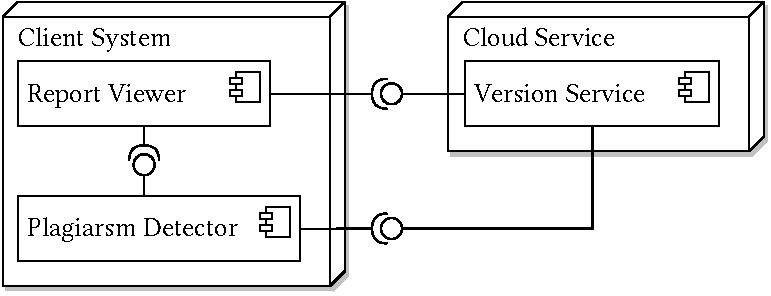
\includegraphics[width=0.7\textwidth]{figures/chapter8/scenario6_jplag.pdf}
    \caption{Simplified component and deployment diagram of the JPlag evaluation scenario.}
    \label{fig:evaluationscenarios:jplag}
\end{figure}

\paragraph{Source}
The \emph{JPlag} evaluation scenario is based on the plagiarism detector of the same name \cite{prechelt_finding_2002}.
Plagiarism detectors compare models or code submissions of programming tasks \cite{saglam_token-based_2022}, e.g., in educational context \cite{saglam_how_2023}, to find suspicious similarities, i.e., plagiarism \cite{saglam_obfuscation-resilient_2024}.
The \emph{JPlag} project, started in 1996, represents one of the most widely-used plagiarism detectors that is resilient against most obfuscation attempts \cite{saglam_obfuscation-resilient_2024,saglam_automated_2024,saglam_detecting_2024,saglam_jplag_2024,saglam_mitigating_2025,schmid_jplag_2025}.
Since 2020, the software architecture of \emph{JPlag} has been re-engineered.
Based on the available documentation of this open-source project \cite{saglam_jplag_2024}, and by cooperating with the current maintainers, we created a \ac{PCM} model of the core functionality.

\paragraph{Description}
\autoref{fig:evaluationscenarios:jplag} shows a simplified diagram of the software architecture.
The \emph{Jplag} software architecture is designed to enable the deployment of the main components, i.e., the \emph{Plagiarism Detector} and the \emph{Report Viewer}, on a client system, a local machine, or a server, to simplify its integration into other products \cite{saglam_jplag_2024}.
Nevertheless, we consider the illustrated deployment to be the most common use case.
The corresponding \ac{PCM} model consists of 3 components with 5 \acp{SEFF} and maps to 3 \acp{TFG} with 65 vertices.

The evaluation scenario comprises three entities: The \emph{Plagiarism Detector}, a \emph{Report Viewer} for displaying analysis results, and a \emph{Version Service} for update notifications.
The \emph{Plagiarism Detector} receives a set of code or model submissions as input and compares them.
This is done internally without any communication to other services \cite{saglam_jplag_2024}.
After the comparison, all results are stored in an archive.
This includes similarity scores between submissions, clusters of similar submissions, or suspiciously similar parts of the submissions.
Because plagiarism detection needs human judgment \cite{saglam_obfuscation-resilient_2024,saglam_detecting_2024}, the results are displayed in a human-readable way using the \emph{Report Viewer}.
The software architecture supports the direct communication between the \emph{Plagiarism Detector} and the \emph{Report Viewer}, but users can also choose to manually load a result archive, e.g., to revisit older comparisons.
The \emph{Report Viewer} is web-based but only operates within the web browser without the need for additional server infrastructure \cite{saglam_jplag_2024}.
Thus, all input remains on the users' \emph{Client System}.
As \emph{Jplag} is subject to continuous development \cite{saglam_jplag_2024}, both components communicate with a \emph{Version Service} to notify users about available updates.

\paragraph{Confidentiality requirements}
Plagiarism detectors like \emph{JPlag} are designed for the educational context, e.g., programming tasks.
Here, student data has to be treated as confidential due to administrative rules and laws like the \acf{GDPR} \cite{council_of_european_union_regulation_2016}.
We interpret this requirement as data flow constraint and restrict that all submissions and all plagiarism detection results shall never leave the client system.
Furthermore, the authors of \emph{JPlag} claim to never collect any usage data from running the software \cite{saglam_jplag_2024}.
Thus, we additionally restrict the \emph{Version Service} to not collect or evaluate any statistical information on the versions in use.

\paragraph{Uncertainty sources}
We use this evaluation scenario to define four uncertainty sources, of which only two negatively affect the system's confidentiality.
This allows for more precise statements about potential false positives in the evaluation \cite{powers_evaluation_2011}.
The first uncertainty source considers the deployment of the \emph{Report Viewer} on the \emph{Client System} or in the cloud.
The second uncertainty source considers the usage of \emph{JPlag} standalone or in conjunction with the \emph{Report Viewer}.
As stated previously, neither uncertainty affects the confidentiality of the software architecture.
The third uncertainty source targets the deployment of the \emph{Plagiarism Detector}, which could be deployed locally or in the cloud.
This could cause sensitive student data to flow to another server, which violates confidentiality---an argument against closed-source plagiarism detection as a service \cite{saglam_obfuscation-resilient_2024,saglam_jplag_2024}.
Last, we add a fourth uncertainty concerning the data collection behavior of the \emph{Version Service}.
As stated previously, evaluating usage data violates confidentiality.





\section{Summary and Outlook}%
\label{sec:evaluationscenarios:summary}

In this chapter, we presented six evaluation scenarios that will be used throughout the evaluation of this thesis.
All evaluation scenarios are based on or related to a case study of a software system that handles confidential data.
The scenarios have different sizes that range from 2 to 21 components, and also have different origins and domains.
For each evaluation scenario, we described its source, software architecture, confidentiality requirements, and uncertainty sources.
All scenarios are modeled using the \ac{PCM}.

The first scenario, the \emph{TravelPlanner}, represents a smartphone app to search and book flights.
The second scenario, the \emph{DistanceTracker}, is a sports or health app that tracks the distance run by a user.
The third scenario, the \emph{OnlineShop}, is an e-commerce application for purchasing items online, introduced in \autoref{ch:runningexample}.
The fourth scenario, the \emph{CoronaWarnApp}, is a contact tracing app developed during the COVID-19 pandemic.
The fifth scenario, \emph{MobilityAsAService}, is a distributed ticketing system based on \ac{DLT} and \acp{TEE}.
The sixth scenario, \emph{JPlag}, is a plagiarism detector, e.g., used for programming tasks in universities.

In sum, these scenarios provide a wide range of different software systems.
Despite their differences in structure and size, they all have to ensure the confidentiality of the processed data.
Furthermore, they are all subject to uncertainty.
We use these scenarios throughout \readingpath{ch:evaluation}.
For more details on the third scenario, the \emph{OnlineShop}, see \readingpath{ch:runningexample}.
For a more detailed view of the components of the fourth scenario, the \emph{CoronaWarnApp}, see \autoref{sec:appendix:cwa}.
Last, we again refer to our data set \cite{dataset} for all uncertainty and architectural models and all data flow constraints.





\section{In Simpler Words}%
\label{sec:evaluationscenarios:simple}

In the last three chapters, we presented the contributions of this thesis.
In our research area, a contribution is an enhancement of the state of the art, e.g., a new or better algorithm, a better way to collect and express knowledge, or a new method.
To investigate the quality of our contributions, we perform an evaluation.
In the discipline of this thesis---software architecture research---many evaluations are based on case studies.
In this chapter, we refer to evaluation scenarios comparable to case studies.

We present six different evaluation scenarios of different sizes and from different domains.
Examples are the health domain, the mobility domain, and e-commerce.
Many of our evaluation scenarios have already been used to evaluate related approaches, e.g., the \emph{TravelPlanner} evaluation scenario.
Other scenarios, e.g., the \emph{CoronaWarnApp} evaluation scenario, are newer but based on well-studied software systems from the real world.
It is important to cover different sizes and domains because otherwise, one could say: \enquote{Your contributions only work for small software systems} or \enquote{Your contributions only work for systems in the mobility domain, but not for others}.
By using various evaluation scenarios, we counteract such---otherwise justified---criticism.
The following chapter will apply our contributions to these evaluation scenarios.

\chapter{Evaluation}%
\label{ch:evaluation}%


In this chapter, we present the evaluation of this thesis.
We choose the joint presentation of the evaluation of all three contributions \C{1}, \C{2}, and \C{3} for increased cohesiveness and clarity.
The evaluation is based on the evaluation scenarios, introduced in \autoref{ch:evaluationscenarios}.

Although all three contributions of this dissertation target confidentiality with regard to uncertainty, they differ in their nature.
For instance, Contribution \C{1} represents a classification, while Contribution \C{3} comprises meta models and analysis approaches.
Thus, we use different evaluation methods such as user studies and the aforementioned evaluation scenarios, which are comparable to case studies.
This matches the findings of \textcite{konersmann_evaluation_2022}, who conducted a \acf{SLR} with 153 papers on the evaluation methods in software architecture research.
For our research object---architecture analysis methods---case studies, motivating examples, and technical experiments represent the most common evaluation methods \cite{konersmann_evaluation_2022}.
In this case, the most commonly investigated properties are effectiveness, functional suitability, and accuracy, which match the presented evaluation.
For most of the evaluation, we focus on the presented analyses, not the presented meta models.
Following the definition of \textcite{stachowiak_allgemeine_1973}, every model has pragmatism, in our case, to serve the analysis.
Thus, evaluating the analysis indirectly also evaluates the underlying models \cite{walter_context-based_2023}.

The evaluation follows a comprehensive \acf{GQM} approach \cite{basili_goal_1994,basili_methodology_1984}.
A \emph{goal} is on the conceptual level and describes a quality to evaluate, i.e., the aforementioned properties to investigate.
An evaluation can have multiple goals.
A \emph{question} is on the operational level and describes how the quality is measured or assessed.
Each goal can have multiple questions.
A \emph{metric} is on the quantitative level and describes the data that is associated with the question.
Each question can have multiple metrics.
A \ac{GQM} plan helps align quality, assessment, and data to minimize the risk of collecting meaningless results \cite{basili_methodology_1984}.
It also helps to structure the evaluation and increases reproducibility.
We number all goals, questions, and metrics and use labels throughout this chapter.

The remainder of this chapter is structured as follows:
We introduce the \ac{GQM} plans for evaluating all contributions \C{1} -- \C{3}.
Then, we present the evaluation design and results for each contribution separately.
We individually discuss the results and threats to validity according to \textcite{runeson_guidelines_2009}.
Last, we give an summary of the evaluation.

\ownpublications{
\fancycite{hahner_architectural_2021}, 
\fancycite{boltz_handling_2022},
\fancycite{walter_architectural_2022},
\fancycite{kaplan_introducing_2022},\linebreak
\fancycite{hahner_model-based_2023}, 
\fancycite{hahner_classification_2023},
\fancycite{hahner_architecture-based_2023},\linebreak
\fancycite{boltz_extensible_2024},
\fancycite{hahner_arcn_2024}
}





\section{Overview}%
\label{sec:evaluation:overview}

We present the individual \ac{GQM} plans of all three contributions.
The first Contribution \C{1} concerns the classification and identification of uncertainty.
We evaluate the structure's suitability, applicability, purpose, and usability.
The second Contribution \C{2} focuses on architecture-based uncertainty impact analysis using uncertainty propagation.
We evaluate the accuracy and effort reduction.
The third Contribution \C{3} comprises four approaches to uncertainty-aware data flow analysis.
We evaluate the accuracy and scalability.

In total, our \ac{GQM} plans comprise 8 goals, 19 questions, and 32 metrics.
In the following, we show the tree of each evaluation goal and then discuss its questions and metrics.


\subsection{Evaluation Plan for the First Contribution}

The first Contribution \C{1} introduces a classification of software-architectural uncertainty regarding confidentiality \cite{hahner_classification_2023}.
Additionally, it includes means to identify uncertainty sources based on an interactive catalog approach \cite{hahner_arcn_2024}.
This approach is tool-supported by \arcen.
The evaluation of this contribution comprises 4 goals, with a total of 12 questions and 16 metrics.
The evaluation is closely aligned to the simultaneously introduced evaluation method for classifications and taxonomies by \textcite{kaplan_introducing_2022}.

\newcommand{\textGi}[0]{Validate the classification \emph{structure's suitability}, whether it permits the appropriate classification of objects under study with the right scope and granularity.}
\newcommand{\textGiQi}[0]{Has the classification an appropriate level of \emph{generality} and granularity?}
\newcommand{\textGiQii}[0]{Is the classification \emph{appropriate}, comprising only necessary classes?}
\newcommand{\textGiQiii}[0]{Is the classification \emph{orthogonal} without overlapping classes?}
\newcommand{\textGiQiMi}[0]{{\emph{laconicity}}(C,\mathcal{R}) = \frac{\sum\nolimits_{R\in \mathcal{R}} \sum\nolimits_{r\in R} \text{laconic}(C,R,r)}{\sum\nolimits_{R\in \mathcal{R}} \lvert R \rvert} \in [0,1]}
\newcommand{\textGiQiMii}[0]{{\emph{lucidity}}(C,\mathcal{R}) = \frac{\sum\nolimits_{c\in C}\,(\min\nolimits_{R\in\mathcal{R}}\,\text{lucid}(C,R,c))}{\lvert C \rvert} \in [0,1]}
\newcommand{\textGiQiiMi}[0]{{\emph{completeness}}(C,\mathcal{R}) = \frac{\sum\nolimits_{R\in \mathcal{R}} \sum\nolimits_{r\in R} \text{complete}(C,R,r)}{\sum\nolimits_{R\in \mathcal{R}} \lvert R\rvert} \in [0,1]}
\newcommand{\textGiQiiMii}[0]{{\emph{soundness}}(C,\mathcal{R}) = \frac{\sum\nolimits_{c\in C}\,(\max\nolimits_{R\in\mathcal{R}}\,\text{sound}(C,R,c))}{\lvert C\rvert} \in [0,1]}
\newcommand{\textGiQiiiMi}[0]{$\emph{orthogonality}(C,\mathcal{R}) \in [0, 1]$, using an orthogonality matrix}
\begin{figure}
    \centering
    \begin{tikzpicture}
      \nodeGtop{1}{\textGi}
      \nodeQtop{1}{1}{\textGiQi}{G1}
      \nodeMtop{1}{1}{1}{$\textGiQiMi$}{Q11}
      \nodeMbottom{1}{1}{2}{$\textGiQiMii$}{M111}
      \nodeQmid{1}{2}{\textGiQii}{M112}
      \nodeMtop{1}{2}{1}{$\textGiQiiMi$}{Q12}
      \nodeMbottom{1}{2}{2}{$\textGiQiiMii$}{M121}
      \nodeQbottom{1}{3}{\textGiQiii}{M122}
      \nodeMonly{1}{3}{1}{\textGiQiiiMi}{Q13}
    \end{tikzpicture}
    \caption{Overview of the \ac*{GQM} plan of the first goal regarding Contribution \C{1}.}
    \label{gqm:plan:g1}
\end{figure}

\paragraph{Goal \goal{1}}\label{gqm:text:g:1}
\autoref{gqm:plan:g1} shows the tree of the first goal.
Following the aforementioned evaluation method \cite{kaplan_introducing_2022}, this goal concerns the classification \emph{structure's suitability}.
This property describes whether a classification is suitable to classify the objects under study.
In our case, the objects under study are sources of uncertainty with respect to confidentiality.
This can be seen as a baseline check as the classification needs to have the right scope and granularity to be suited.
We also motivated the classification in \autoref{ch:classification} with the lack of suitable taxonomies.
We consider three evaluation questions:

\begin{enumerate}[leftmargin=\GQMquestionsIndent]
  \item[\question{1}{1}] \textGiQi 
  \item[\question{1}{2}] \textGiQii
  \item[\question{1}{3}] \textGiQiii
\end{enumerate}

\phantomsection
\label{gqm:text:q:1:1}
The first Question \question{1}{1} asks about the \emph{generality}, where we evaluate the granularity, i.e. if the classification is not too general but also not too specific.
The right level of granularity is important as a classification group objects under study into classes---a too-low number of classes reduces the usefulness of this information, while a high number too-high number of classes introduces noise and makes the classification results hard to understand.
To this end, the evaluation method reuses metrics used to evaluate conceptual models with respect to tools \cite{kaplan_introducing_2022,ananieva_conceptual_2020}.
The \emph{laconicity} (\metric{1}{1}{1}\label{gqm:text:m:1:1:1}) measures the fraction of terms that are uniquely describable.
Given a classification \emph{C}, a finite set of objects under study $\mathcal{R}$, with $R \in \mathcal{R}$ being an object under study with relevant terms $r \in \mathcal{R}$, then $m^C_R \subseteq C \times R$ describes the relation of classes $c \in C$ to relevant terms $r \in R$.
In our classification, we use the term \emph{option} to refer to classes, e.g., \emph{Behavior} uncertainty and \emph{Scenario} uncertainty are two of the 27 options of our classification.
A class is laconic, if there is at most one $c \in C$ with $(c,r) \in m^C_R$.
Based on this, we denote:

\begin{equation*}
  \textGiQiMi
\end{equation*}

\phantomsection
A low laconicity indicates a too fine-grained classification with potentially too many classes to describe the object under study.
Put simply, a concept of an object under study should be only describable using a single class, otherwise the classification structure's suitability could be decreased.
For instance, if we have one object under study, one term that represents \emph{Behavior} uncertainty, and one class to describe it, this class is laconic, thus ${\emph{laconicity}}(C,\mathcal{R}) = \frac{1}{1} = 1.0$.
If we add five additional options to describe \emph{Behavior} uncertainty without need, this decreases the laconicity; in this case to zero, as $\frac{0}{1} = 0.0$

The \emph{lucidity} (\metric{1}{1}{2}\label{gqm:text:m:1:1:2}) measures the opposite, i.e., the fraction of classes that describe exactly one term.
A class is lucid, if there is at most one $r \in R$ with $(c,r) \in m^C_R$:

\begin{equation*}
  \textGiQiMii
\end{equation*}

A low lucidity indicates a too-coarse-grained classification that could overestimate classes and not distinguish enough.
For instance, if we have five three classes, where two describe only one term, e.g., \emph{Behavior} and \emph{External} uncertainty, but the third class does describes both terms, then ${\emph{lucidity}}(C,\mathcal{R}) = \frac{(1 + 1 + 0)}{3} = \frac{2}{3}$.
Put simply, a class of classification should only describe a single concept of an object under study.
A good trade-off regarding granularity is important because we want to be able to differentiate between uncertainties without assigning a separate class to every instance.
Also, the granularity must fit the purpose of classifying software-architectural uncertainty regarding confidentiality.

\phantomsection
\label{gqm:text:q:1:2}
The second Question \question{1}{2} asks about the \emph{appropriateness}, where we evaluate whether the classification has enough categories without having unnecessary categories.
On the one hand, we shall be able to classify every software-architectural uncertainty that can have an impact on confidentiality.
On the other hand, categories and options that are never used, should not be maintained.
Similarly to the metrics used for Question \question{1}{1}, we reuse metrics from the evaluation of conceptual models \cite{kaplan_introducing_2022,ananieva_conceptual_2020}.
The \emph{completeness} (\metric{1}{2}{1}\label{gqm:text:m:1:2:1}) measures the fraction of complete terms over all objects under study.
Each term of all objects under study should be covered by at least one class, otherwise the completeness is reduced.
A term is $r \in R$ is complete, if there is at least one $c \in C$ with $(c,r) \in m^C_R$:

\begin{equation*}
  \textGiQiiMi
\end{equation*}

\phantomsection
A low completeness indicates missing classes as not all important properties of all objects under study can be described.
Put simply, a classification that cannot be used to describe an object is not complete.
For instance, if we remove the option of \emph{Behavior} uncertainty we cannot classify many uncertainty sources appropriately.
The \emph{soundness} (\metric{1}{2}{2}\label{gqm:text:m:1:2:2}) measures the fraction of sound classes in the classification.
Each class should be required to describe at least one object under study, otherwise it is unnecessary can be removed.
A class $c \in C$ is sound, if there is at least one $r \in R$ with $(c,r) \in m^C_R$.
We denote: 

\begin{equation*}
  \textGiQiiMii
\end{equation*}

A low soundness indicates unnecessary classes as not all classes are required to describe all objects under study.
Put simply, a classification with low soundness introduces noise and complicates the classification process.
For instance, if we add an option called \emph{Color} uncertainty that describes the effect of the color of a button in the user interface on confidentiality, the soundness is reduced\footnote{Note that we do not state that there is no effect of the color of a button on confidentiality, think of, for instance, phishing attacks. However, the relevance for software-architectural uncertainty is negligible.}.

\phantomsection
\label{gqm:text:q:1:3}
The third Question \question{1}{3} asks about the \emph{orthogonality}, where we evaluate whether the classification has overlapping categories.
A lack of orthogonality implies that options depend on each other and can be removed to increase preciseness.
To measure \emph{orthogonality} (\metric{1}{3}{1}\label{gqm:text:m:1:3:1}), we construct an orthogonality matrix.
The classes of a classification denote both the columns and rows of a $n \times n$ matrix.
A cell is filled with a zero if two classes are independent or a one if the class in the row implies the class in the column.
The entries on the main diagonal are not considered as the dependency relation between two classes is irreflexive.
The orthogonality is the fraction of $\abs{C}^2 - \abs{C}$ minus the number of cells filled with ones and the cell count.
A low orthogonality, i.e., many dependencies between classes, indicates unclear boundaries \cite{bedford_evaluating_2013}.
For instance, if \emph{Behavior} uncertainty implicates \emph{Scenario} uncertainty, the orthogonality is decreased.
Overall, a classification with bad structural quality yields ambiguous results and should be adapted.


\newcommand{\textGii}[0]{Validate the classification's \emph{applicability}, whether it is understandable, usable, and yields consistent results when employed by different users.}
\newcommand{\textGiiQi}[0]{Does using the classification produce consistent and thus \emph{reliable} results?}
\newcommand{\textGiiQii}[0]{Does using the classification produce \emph{correct} results?}
\newcommand{\textGiiQiii}[0]{Is the classification \emph{easy to use} and easy to understand?}
\newcommand{\textGiiQiMi}[0]{Relative size of the largest annotator $\emph{consensus} \in [0,1]$}
\newcommand{\textGiiQiiMi}[0]{Correctness of annotators' results, $\recallFormulaFull$}
\newcommand{\textGiiQiiiMi}[0]{\acf{SUS} $\in [0,100]$}
\begin{figure}
    \centering
    \begin{tikzpicture}
      \nodeGtop{2}{\textGii}
      \nodeQtop{2}{1}{\textGiiQi}{G2}
      \nodeMonly{2}{1}{1}{\textGiiQiMi}{Q21}
      \nodeQmid{2}{2}{\textGiiQii}{M211}
      \nodeMonly{2}{2}{1}{\textGiiQiiMi}{Q22}
      \nodeQbottom{2}{3}{\textGiiQiii}{M221}
      \nodeMonly{2}{3}{1}{\textGiiQiiiMi}{Q23}
    \end{tikzpicture}
    \caption{Overview of the \ac*{GQM} plan of the second goal regarding Contribution \C{1}.}
    \label{gqm:plan:g2}
\end{figure}

\paragraph{Goal \goal{2}}\label{gqm:text:g:2}
\autoref{gqm:plan:g2} shows the tree of the second goal that is also based on the aforementioned evaluation method \cite{kaplan_introducing_2022}.
We focus on the classification's \emph{applicability}, i.e., whether the classification is understandable and usable, see \emph{Usable Security} \cite{sasse_usable_2005}.
\textcite{kaplan_introducing_2022} propose to conduct a user study.
A classification with suitable structural quality (\goal{1}) can still be bad if does not yield consistent results results by different users.
Classifications are meant to communicate.
We consider three evaluation questions:

\begin{enumerate}[leftmargin=\GQMquestionsIndent]
  \item[\question{2}{1}] \textGiiQi 
  \item[\question{2}{2}] \textGiiQii
  \item[\question{2}{3}] \textGiiQiii
\end{enumerate}

\phantomsection
\label{gqm:text:q:2:1}
The first Question \question{2}{1} asks about the \emph{reliability}, where we evaluate whether different user's results are consistent when applying the classification.
An ambiguous classification with inconsistent results indicates a lack of preciseness regarding classes, categories, or their description.
Here, we measure the relative size of the largest \emph{consensus} (\metric{2}{1}{1}\label{gqm:text:m:2:1:1}) among all users of the classification.
A low consensus indicates a lack of comprehensibility of class names, categories, and their descriptions.
For instance, if three out of five users classify an uncertainty as \emph{Behavior} uncertainty, and the other two users classify it as \emph{Component} uncertainty, the largest consensus is three out of five.

\phantomsection
\label{gqm:text:q:2:2}
The second Question \question{2}{2} asks about the \emph{correctness} of the user's results by applying the classification.
This can be evaluated by comparing the individual results to a predefined gold standard.
As the comparison of users' and experts' results resembles a binary classification, we can apply the terminology of true positives (TP), false positives (FP), true negatives (TN), and false negatives (FN) \cite{powers_evaluation_2011,van_rijsbergen_information_1979}.
We measure the true positive rate, i.e., the \emph{recall} (\metric{2}{2}{1}\label{gqm:text:m:2:2:1}), which is calculated as:

\begin{equation*}
  \recallFormula
\end{equation*}

A low recall indicates that users could not benefit from applying the classification.
For instance, if only one out of five users correctly identifies an uncertainty source as \emph{Behavior} uncertainty, this indicates a lack of understandability of this option.

\phantomsection
\label{gqm:text:q:2:3}
The third Question \question{2}{3} asks about the \emph{ease of use} of the classification.
Besides the objective measures of concise and correct classification results, this question focuses on the perceived quality, which is subjective.
\textcite{kaplan_introducing_2022} recommend using a standardized questionnaire, e.g., the \acf{SUS} \cite{lewis_system_2018} (\metric{2}{3}{1}\label{gqm:text:m:2:3:1}).
This questionnaire comprises ten questions regarding the usability, perceived complexity, and ease of use.
Each question can be answered on a scale from 1 to 5, which is the base to calculate a score between 0 and 100 \cite{lewis_system_2018}.
A low score indicates a lack of usability or understandability that can be addressed, e.g., by increasing the consistency of naming classes or by improving textual descriptions.
Additionally, participants can be asked if they understand the categories and find them helpful and whether they experienced a knowledge gain by participating in the user study.
Overall, a classification has to yield consistent and correct results without requiring too much effort in order to be usable.


\newcommand{\textGiii}[0]{Validate the classification's \emph{purpose}, i.e., the classification's quality and relevance in comparison to existing classifications and taxonomies.}
\newcommand{\textGiiiQi}[0]{Is the classification \emph{relevant}, comprising only necessary categories?}
\newcommand{\textGiiiQii}[0]{Is the classification \emph{novel}, having the right degree of new categories?}
\newcommand{\textGiiiQiii}[0]{Is the classification \emph{significant}, enabling a more precise description?}
\newcommand{\textGiiiQiMi}[0]{Fraction of relevant classes and categories}
\newcommand{\textGiiiQiiMi}[0]{\emph{innovation}(C,\mathcal{T}) = \frac{\sum\nolimits_{c\in C} \min_{T\in\mathcal{T}} new(C,T,c) }{\lvert C \rvert} \in [0,1]}
\newcommand{\textGiiiQiiMii}[0]{\emph{adaptation}(C,\mathcal{T}) = \frac{\sum\nolimits_{c\in C} \max_{T\in\mathcal{T}} adapted(C,T,c) }{\lvert C \rvert} \in [0,1]}
\newcommand{\textGiiiQiiiMi}[0]{\emph{classificationDelta}(C,\mathcal{T},\mathcal{R}) = \frac{\lvert\sim_C\rvert - (\max_{T\in \mathcal{T}} \lvert\sim_T\rvert)}{\lvert\mathcal{R}\rvert} \in [-1,1]}
\begin{figure}
    \centering
    \begin{tikzpicture}
      \nodeGtop{3}{\textGiii}
      \nodeQtop{3}{1}{\textGiiiQi}{G3}
      \nodeMonly{3}{1}{1}{\textGiiiQiMi}{Q31}
      \nodeQmid{3}{2}{\textGiiiQii}{M311}
      \nodeMtop{3}{2}{1}{$\textGiiiQiiMi$}{Q32}
      \nodeMbottom{3}{2}{2}{$\textGiiiQiiMii$}{M321}
      \nodeQbottom{3}{3}{\textGiiiQiii}{M322}
      \nodeMonly{3}{3}{1}{$\textGiiiQiiiMi$}{Q33}
    \end{tikzpicture}
    \caption{Overview of the \ac*{GQM} plan of the third goal regarding Contribution \C{1}.}
    \label{gqm:plan:g3}
\end{figure}

\paragraph{Goal \goal{3}}\label{gqm:text:g:3}
\autoref{gqm:plan:g3} shows the tree of the third goal.
Like the previous goals, this goal follows the evaluation method for taxonomies \cite{kaplan_introducing_2022}.
This goal considers the classification's \emph{purpose}, i.e., its relevance and improvement compared to the state of the art\footnote{One could question whether \emph{purpose} is a property that can be quantitatively evaluated or whether it is better to argue when discussing related work. We agree with this point of view. Nevertheless, we use the term \emph{purpose} in this evaluation to remain consistent with the evaluation method of \textcite{kaplan_introducing_2022}.}.
A classification with a suitable structure (\goal{1}) and applicability (\goal{2}) could still lack novelty.
Then, reusing existing classifications is preferred \cite{kaplan_introducing_2022}.
We consider three questions:

\begin{enumerate}[leftmargin=\GQMquestionsIndent]
  \item[\question{3}{1}] \textGiiiQi 
  \item[\question{3}{2}] \textGiiiQii
  \item[\question{3}{3}] \textGiiiQiii
\end{enumerate}

\phantomsection
\label{gqm:text:q:3:1} 
The first question \question{3}{1} asks about the \emph{relevance} of the classification, where we evaluate whether each category helps the purpose of the classification.
In our case, the purpose is to understand the impact of uncertainty sources on confidentiality.
Here, we question the relevance of all classes $c \in C$ and also of all categories.
We measure the \emph{relevance} (\metric{3}{1}{1}\label{gqm:text:m:3:1:1}) as fraction of relevant classes and categories.
Note that this metric is not similar to the comparison of classes and terms of Goal \goal{1} but considers the relevance of classes and categories as means to an end.
A low relevance indicates that the classification contains irrelevant elements that should be removed.

\phantomsection
\label{gqm:text:q:3:2}
The second question \question{3}{2} asks about the \emph{novelty} of the classification compared to previous classifications and taxonomies, i.e., the state of the art.
While a research increment should contain some degree of novelty, it should also refer to existing concepts to increase validity.
Thus, we measure both how many classes and categories are new and also how many of them are adapted.
The trade-off between both measures depends on the purpose, e.g., a classification that combines existing classifications has a lower fraction of novel classes and categories.
To this end, we measure \emph{innovation} (\metric{3}{2}{1}\label{gqm:text:m:3:2:1}) and \emph{adaption} (\metric{3}{2}{2}\label{gqm:text:m:3:2:2}).
Given a classification \emph{C} with classes and categories $c \in C$, a finite set of previous classifications $T\in \mathcal{T}$ with classes and categories $d\in T$, where $\simeq\ \subseteq C \times T$ denotes that a class or category is adapted.
Then, a class or category is new if $c \neq d$ and $c \not\simeq d$ for all $d\in T$.
Otherwise, a class or category $c\in C$ is adapted if $c \simeq d$ for any $d\in T$.
Based on this, we denote:

\begin{equation*}
  \textGiiiQiiMi
\end{equation*}

A low innovation indicates a small difference compared to state of the art.
However, this has to be interpreted with regard to the purpose of the classification, as discussed above.
Thus, there is no \emph{best} value.
Nevertheless, measuring the innovation and providing arguments for the measured value helps clarify the classification's purpose.
Extreme values close to zero or one are the most difficult to justify here.
For instance, just copying an existing taxonomy would yield an innovation of zero.
Additionally, we denote:

\begin{equation*}
  \textGiiiQiiMii
\end{equation*}

A low adaptation indicates a large difference compared to the state of the art.
Similarly to the innovation, this can be desirable.
Nevertheless, building on the state of the art may increase the validity.
For instance, a previous taxonomy of uncertainty \cite{perez-palacin_uncertainties_2014} also referred to existing classifications.
Both metrics indicate the strength of the relation of the classification to other taxonomies.

\phantomsection
\label{gqm:text:q:3:3} 
The third question \question{3}{3} asks about the \emph{significance}, where we evaluate whether the classification enables a more precise description of the objects under study with respect to its purpose.
Put simply, as our classification is aimed towards describing uncertainty with respect to confidentiality, it should enable a more precise description in this area than the state of the art.
Given a classification $C$, a finite set of previous classifications $T\in \mathcal{T}$, and a finite set of objects under study $\mathcal{R}$, $\sim_T$ denotes that a pair of objects under study are classified identically with respect to the classification $T$, forming an equivalence class.
We measure the \emph{classificationDelta} (\metric{3}{3}{1}\label{gqm:text:m:3:3:1}), that describes whether or not a classification is able to yield more and smaller equivalence class than the most precise existing classification, which indicates a higher precision.
We denote:

\begin{equation*}
  \textGiiiQiiiMi
\end{equation*}

A negative delta indicates that an already existing classification is more precise and could be used instead.
A positive delta indicates an increase in preciseness, which is what we aim for.
For instance, if we provide three relevant options to describe uncertainty sources where other taxonomies only provide one, the delta can be increased.
However, only optimizing for the classification delta impairs other metrics, e.g., regarding the structure's suitability (\goal{1}), and applicability (\goal{2}).
Thus, a good trade-off with respect to the purpose of the classification has to be achieved.
If the classification fails the evaluation of purpose, it represents no significant improvement over the state of the art.


\newcommand{\textGiv}[0]{Validate the catalog approach's \emph{usability} in identifying and understanding uncertainty sources in software architectures.}
\newcommand{\textGivQi}[0]{Does the catalog support \emph{identifying} and describing uncertainty sources?}
\newcommand{\textGivQii}[0]{Does the catalog support \emph{collaboration} and discussion?}
\newcommand{\textGivQiii}[0]{Is the catalog \emph{easy to use} and provides a good user experience?}
\newcommand{\textGivQiMi}[0]{Percentage of correct answers $\in [0,1]$}
\newcommand{\textGivQiiMi}[0]{Percentage of correct answers $\in [0,1]$}
\newcommand{\textGivQiiiMi}[0]{\acf{SUS} $\in [0,100]$}
\newcommand{\textGivQiiiMii}[0]{Average \emph{usefulness and intuitiveness} rating $\in [1,4]$}
\begin{figure}
    \centering
    \begin{tikzpicture}
      \nodeGtop{4}{\textGiv}
      \nodeQtop{4}{1}{\textGivQi}{G4}
      \nodeMonly{4}{1}{1}{\textGivQiMi}{Q41}
      \nodeQmid{4}{2}{\textGivQii}{M411}
      \nodeMonly{4}{2}{1}{\textGivQiiMi}{Q42}
      \nodeQbottom{4}{3}{\textGivQiii}{M421}
      \nodeMtop{4}{3}{1}{\textGivQiiiMi}{Q43}
      \nodeMbottom{4}{3}{2}{\textGivQiiiMii}{M431}
    \end{tikzpicture}
    \caption{Overview of the \ac*{GQM} plan of the fourth goal regarding Contribution \C{1}.}
    \label{gqm:plan:g4}
\end{figure}

\paragraph{Goal \goal{4}}\label{gqm:text:g:4}
\autoref{gqm:plan:g4} shows the tree of the fourth goal.
This goal aims towards the uncertainty source catalog, which is realized with \arcen.
We evaluate the \emph{usability} of the catalog approach regarding identifying and understanding uncertainty sources.
These are also the desired qualities of the approach, described in \autoref{ch:classification}.
To this end, a user study is the preferred evaluation approach.
We consider three evaluation questions:

\begin{enumerate}[leftmargin=\GQMquestionsIndent]
  \item[\question{4}{1}] \textGivQi 
  \item[\question{4}{2}] \textGivQii
  \item[\question{4}{3}] \textGivQiii
\end{enumerate}

\phantomsection
\label{gqm:text:q:4:1}
The first Question \question{4}{1} asks about \emph{identifying} uncertainty and whether the catalog helps in identifying and describing uncertainty sources.
This question is central as the catalog addresses the \acf{UAP}, i.e., the problem of identifying uncertainty sources \cite{hahner_arcn_2024}.
We measure the \emph{correctness} (\metric{4}{1}{1}\label{gqm:text:m:4:1:1}) as percentage of correct answers.
Based on a gold standard of previously introduced uncertainty sources, we rate each answer as either correct or incorrect.
A low correctness indicates that the catalog does not sufficiently support the identification of unknown uncertainty sources.
For instance, if four out of five uncertainty sources in an architectural model were identified correctly, a high correctness is achieved.

\phantomsection
\label{gqm:text:q:4:2}
The second Question \question{4}{2} asks about the \emph{collaboration} aspect of the catalog, where we evaluate whether users are able to retrieve information from online discussions about uncertainty sources.
Besides supporting the identification process, the catalog has a collaborative aspect by providing the means to share knowledge about uncertainty between software architects and institutions, see \autoref{sec:classification:collaboration}.
We measure the \emph{correctness} (\metric{4}{2}{1}\label{gqm:text:m:4:2:1}) as percentage of correct answers.
This approach is the same as in answering the previous Question \question{4}{1}.
A low correctness indicates that the catalog does not sufficiently support collaboration between users.
For instance, if only one out of five users refers to additional material like online discussions, the catalog falls short of promoting collaboration.

\phantomsection
\label{gqm:text:q:4:3}
The third Question \question{4}{3} asks about the \emph{ease of use} and the user experience using the catalog and its tool support \arcen.
This question is similar to \question{2}{3} of evaluating the ease of use of the classification.
Furthermore, this enables the comparison of the results regarding the usability of the classification and the catalog approach.
We measure the users' satisfaction  using the \acf{SUS} \cite{lewis_system_2018} (\metric{4}{3}{1}\label{gqm:text:m:4:3:1}).
This questionnaire comprises ten questions and yields a score between 0 and 100, as discussed with Question \question{2}{3}.
A low score indicates improvement potential regarding the user experience of the catalog and its realization.
Additionally, we measure the \emph{usefulness} and \emph{intuitiveness} (\metric{4}{3}{2}\label{gqm:text:m:4:3:2}).
We ask about the perceived quality of different aspects of the catalog, like examples, or explanations with respect to the underlying classification \cite{hahner_classification_2023} on a scale from 1 to 4.
We average the individual results for each question separately.
A low score helps to identify aspects or features of the catalog approach that do not help in identifying uncertainty sources.
This complements the \ac{SUS} and enables us to derive more precise findings on the catalog approach.
For instance, outliers can be used to improve the catalog by either enhancing or removing the aspect or feature.
In sum, this goal comprises both objective and subjective measures to evaluate the catalog's usability.


\subsection{Evaluation Plan for the Second Contribution}

The second Contribution \C{2} introduces an architecture-based uncertainty impact analysis regarding confidentiality \cite{hahner_architecture-based_2023}.
The architectural propagation of uncertainty is related to change impact analysis \cite{rostami_architecture-based_2015,rostami_architecture-based_2017,busch_architecture-based_2020}.
This approach is tool-supported by \uia.
The evaluation of this contribution comprises 2 goals, with a total of 2 questions and 5 metrics.
The evaluation is closely aligned with the evaluation of change impact analysis \cite{rostami_architecture-based_2017}.

\newcommand{\textGv}[0]{Validate the \emph{accuracy} of the impact set that represents the result of uncertainty impact analysis, i.e., the quality of the prediction of confidentiality violations.}
\newcommand{\textGvQi}[0]{How \emph{precise and complete} is the result compared to manual analysis?}
\newcommand{\textGvQiMi}[0]{$\precisionFormulaFull$}
\newcommand{\textGvQiMii}[0]{$\recallFormulaFull$}
\newcommand{\textGvQiMiii}[0]{$F_{1} = 2 \cdot \frac{\text{precision} \cdot \text{recall}}{\text{precision} + \text{recall}} \in [0,1]$}
\begin{figure}
    \centering
    \begin{tikzpicture}
      \nodeGtop{5}{\textGv}
      \nodeQonly{5}{1}{\textGvQi}{G5}
      \nodeMtop{5}{1}{1}{\textGvQiMi}{Q51}
      \nodeMmid{5}{1}{2}{\textGvQiMii}{M511}
      \nodeMbottom{5}{1}{3}{\textGvQiMiii}{M512}
    \end{tikzpicture}
    \caption{Overview of the \ac*{GQM} plan of the fifth goal regarding Contribution \C{2}.}
    \label{gqm:plan:g5}
\end{figure}

\paragraph{Goal \goal{5}}\label{gqm:text:g:5}
\autoref{gqm:plan:g5} shows the tree of the fifth goal.
This goal focuses on the \emph{accuracy} of the uncertainty impact analysis.
This analysis yields an impact set that represents an overestimation of the potential impact of uncertainty on confidentiality, see \autoref{ch:impactanalysis}.
Thus, the central quality is to provide an accurate impact set that predicts potential confidentiality violations with only little overestimation \cite{bohner_software_2002}.
An impact analysis that extensively overestimates the impact is bad---however, an impact analysis that underestimates the impact is worse \cite{hahner_architecture-based_2023}.
We consider one central evaluation question:

\begin{enumerate}[leftmargin=\GQMquestionsIndent]
  \item[\question{5}{1}] \textGvQi 
\end{enumerate}

\phantomsection
\label{gqm:text:q:5:1}
The Question \question{5}{1} asks about the \emph{precision} and \emph{completeness} of the impact set as the result of the uncertainty impact analysis.
We compare this result to confidentiality violations identified by architecture-based confidentiality analysis \cite{seifermann_detecting_2022,boltz_extensible_2024}.
We use the common terminology \cite{rostami_architecture-based_2017} introduced in \autoref{sec:impactanalysis:pcmpropagation} and call the \emph{actual impact set}, the set of elements that are affected by uncertainty and would violate confidentiality in a manual confidentiality analysis.
We consider the actual impact set to be the ideal result.
The uncertainty impact analysis yields an \emph{impact set of uncertainty}, i.e., the set of elements that are potentially affected.
Similarly to \question{2}{2}, the comparison of these sets enables the application of the terminology known from binary classification, i.e., true positives (TP), false positives (FP), true negatives (TN), and false negatives (FN) \cite{powers_evaluation_2011,van_rijsbergen_information_1979}.
An element of the impact set represents a true positive (TP) if it violates confidentiality and is thus also in the actual impact set.
If the element is only in the impact set, it is a false positive (FP).
If an element of the actual impact set is not found by our analysis, it represents a false negative (FN).
We use this terminology in the three metrics used to answer Question \question{5}{1}.
First, we measure the precision (\metric{5}{1}{1}\label{gqm:text:m:5:1:1}), which is calculated as:

\begin{equation*}
  \precisionFormula
\end{equation*}

\phantomsection
A low precision indicates a large overestimation.
This makes the interpretation of the impact set more difficult as software architects have to manually filter our potential false positives.
In the worst case, a lack of precision can lead to an unusable impact set.
For instance, if a confidentiality violation occurs in a database component but the full software system is part of the impact set, this renders the result ineffective.
Second, we measure the \emph{recall} (\metric{5}{1}{2}\label{gqm:text:m:5:1:2}), which is calculated as:

\begin{equation*}
  \recallFormula
\end{equation*}

\phantomsection
A low recall indicates that the impact set misses elements from the actual impact set, i.e., underestimates potential confidentiality violations.
As discussed previously, we prefer a lower precision in order to maximize the recall, as the impact analysis only represents an early estimation of the potential impact.
After inspecting the impact set, software architects can identify confidentiality violations due to uncertainty using uncertainty-aware data flow analysis, see the procedure descried in \autoref{sec:overview:procedure}.
For instance, if the impact set overestimates the impact in a critical system part, further analysis steps might be required.
Third, we measure the \emph{F\textsubscript{1}} score (\metric{5}{1}{3}\label{gqm:text:m:5:1:3}), which is calculated as:

\begin{equation*}
  F_{1} = 2 \cdot \frac{\text{precision} \cdot \text{recall}}{\text{precision} + \text{recall}} \in [0,1]
\end{equation*}

The F\textsubscript{1} score is the harmonic mean of precision and recall and serves as indicator on the overall accuracy.
For all metrics, 0 represents the worst, and 1 is the best possible value.
Put simply, this goal validates the \emph{accuracy} by comparing the prediction of confidentiality violations to actual existing confidentiality violations.


\newcommand{\textGvi}[0]{Validate the \emph{effort reduction} of the uncertainty impact analysis, i.e., how many \acs{DFD} nodes have to be manually considered by software architects.}
\newcommand{\textGviQi}[0]{How large is the \emph{effort reduction} compared to manual analysis?}
\newcommand{\textGviQiMi}[0]{Ratio of the actual impact set, $ratio_{actual} = \frac{TP + FN}{n} \in [0,1]$}
\newcommand{\textGviQiMii}[0]{Ratio of the uncertainty impact set, $ratio_{impact} = \frac{TP + FP}{n} \in [0,1]$}
\begin{figure}
    \centering
    \begin{tikzpicture}
      \nodeGtop{6}{\textGvi}
      \nodeQonly{6}{1}{\textGviQi}{G6}
      \nodeMtop{6}{1}{1}{\textGviQiMi}{Q61}
      \nodeMbottom{6}{1}{2}{\textGviQiMii}{M611}
    \end{tikzpicture}
    \caption{Overview of the \ac*{GQM} plan of the sixth goal regarding Contribution \C{2}.}
    \label{gqm:plan:g6}
\end{figure}

\paragraph{Goal \goal{6}}\label{gqm:text:g:6}
\autoref{gqm:plan:g6} shows the tree of the sixth goal.
This goal considers the \emph{effort reduction} of the uncertainty impact analysis.
The impact analysis serves software architects to initially understand the impact of uncertainty to plan further analysis and mitigation steps, see \autoref{sec:overview:procedure}.
Especially in large software systems, manual analysis is bothersome and erroneous \cite{seifermann_data-driven_2019}.
Thus, an impact analysis should reduce the effort of, in the worst case, manually inspecting every element of the software architecture.
This approach to evaluating effort reduction stems from the evaluation of change impact analysis \cite{rostami_architecture-based_2017,busch_architecture-based_2020} and also has been used for other propagation-based analyses in software architecture \cite{walter_architectural_2022,hahner_architecture-based_2024}.
As we focus on confidentiality and data flow-based analysis, we refer to every node of a \acf{DFD} that represents the architectural model, see \autoref{sec:confidentialityanalysis:framework}.
We consider one central evaluation question:

\begin{enumerate}[leftmargin=\GQMquestionsIndent]
  \item[\question{6}{1}] \textGviQi 
\end{enumerate}

\phantomsection
\label{gqm:text:q:6:1}
The Question \question{6}{1} asks about the \emph{effort reduction} compared to manual analysis.
With manual analysis, we mean manually considering every element of the architecture, i.e., every \ac{DFD} node.
Here, confidentiality violations identified by architecture-based confidentiality analysis \cite{seifermann_detecting_2022,boltz_extensible_2024} represent the baseline, similarly to the previous Question \question{5}{1}.
This enables us to reuse the terminology of binary classification \cite{powers_evaluation_2011,van_rijsbergen_information_1979}.
Elements that actually contain confidentiality violations represent true positives (TP), elements that were missed represent false negatives (FN), and overestimated elements represent false positives (FP).
Independent of the use of an impact analysis, software architects have to consider at least all nodes that represent confidentiality violations.
Similar to change impact analysis \cite{rostami_architecture-based_2017}, we measure the \emph{ratio of the actual impact set} (\metric{6}{1}{1}\label{gqm:text:m:6:1:1}), which is calculated as:

\begin{equation*}
  ratio_{actual} = \frac{TP + FN}{n}
\end{equation*}

\phantomsection
Here, \emph{n} represents the total number of \ac{DFD} nodes.
A low ratio indicates that only a few elements of the \ac{DFD} show confidentiality violations, which represents the ideal results of the impact analysis.
For instance, a \ac{DFD} with 10 nodes could have two nodes that violate confidentiality.
In the case of a perfect recall, the set of elements containing confidentiality violations forms a lower bound to the required effort.
Using the terminology introduced in \autoref{sec:impactanalysis:pcmpropagation} and also used in the previous Question \question{5}{1}, the actual impact set should be a subset of the impact set.
To compare this minimally required effort to the effort of the impact analysis, we additionally measure the \emph{ratio of the uncertainty impact set} (\metric{6}{1}{2}\label{gqm:text:m:6:1:2}), which is calculated as:

\begin{equation*}
  ratio_{impact} = \frac{TP + FP}{n}
\end{equation*}

A low ratio indicates that only a few elements are potentially impacted by uncertainty.
For instance, a \ac{DFD} with 10 nodes could have an uncertainty impact set comprising 3 of its nodes.
The two metrics not only enable quantifying the effort reduction but also show the overestimation of the impact analysis.
In the case of the \ac{DFD} with 10 nodes, 2 confidentiality violations, and 3 elements in the impact set, the overestimation of 1 node becomes visible.
Although we expect the ratio of the actual impact set to be lower than the ratio of the uncertainty impact set, this does not imply that uncertainty impact analysis does not reduce the effort compared to manual confidentiality analysis.
As discussed in \autoref{sec:overview:procedure} and \autoref{ch:confidentialityanalysis}, uncertainty-aware confidentiality analysis requires more detailed models and, thus, modeling effort by software architects.
With a reasonable overestimation, uncertainty impact analysis still reduces the overall effort with regard to a first assessment of confidentiality under uncertainty.
In sum, the comparison of confidentiality analysis and uncertainty impact analysis enables a thorough evaluation of accuracy and effort reduction.


\subsection{Evaluation Plan for the Third Contribution}

The third Contribution \C{3} introduces four approaches to uncertainty-aware data flow analysis to identify confidentiality violations with respect to uncertainty.
We introduce different approaches that differ in modeling and analyzing uncertainty within the architectural model.
The fourth approach is tool-supported by \abunai.
The evaluation comprises 2 goals, with a total of 5 questions and 11 metrics.
The evaluation is related to the evaluation of architecture-based confidentiality analysis \cite{walter_context-based_2023,seifermann_architectural_2022}.

\newcommand{\textGvii}[0]{Validate the \emph{scalability} of the uncertainty-aware data flow analyses that correlate with the number of considered \acsp{TFG} in the analysis.}
\newcommand{\textGviiQi}[0]{How does the \emph{scalability} of the uncertainty-aware analyses compare?}
\newcommand{\textGviiQiMi}[0]{Scalability of scenario-aware analysis, $\emph{scalability\textsubscript{scenario}}=\frac{N_{S}}{\abs{U}}$}
\newcommand{\textGviiQiMii}[0]{Scalability of graph-aware analysis, $\emph{scalability\textsubscript{graph}}=\frac{N_{G}}{\abs{U}}$}
\newcommand{\textGviiQiMiii}[0]{Scalability of impact-aware analysis, $\emph{scalability\textsubscript{impact}}=\frac{N_{I}}{\abs{U}}$}
\begin{figure}
    \centering
    \begin{tikzpicture}
      \nodeGtop{7}{\textGvii}
      \nodeQonly{7}{1}{\textGviiQi}{G7}
      \nodeMtop{7}{1}{1}{\textGviiQiMi}{Q71}
      \nodeMmid{7}{1}{2}{\textGviiQiMii}{M711}
      \nodeMbottom{7}{1}{3}{\textGviiQiMiii}{M712}
    \end{tikzpicture}
    \caption{Overview of the \ac*{GQM} plan of the seventh goal regarding Contribution \C{3}.}
    \label{gqm:plan:g7}
\end{figure}

\paragraph{Goal \goal{7}}\label{gqm:text:g:7}
\autoref{gqm:plan:g7} shows the tree of the seventh goal.
This goal investigates the \emph{scalability} of the different approaches to uncertainty-aware data flow analysis, introduced in \autoref{ch:confidentialityanalysis}.
Although design time analyses are not as critical as runtime analyses regarding the execution time, they still can face combinatorial explosion \cite{koziolek_automated_2011}.
The underlying data flow analysis framework, introduced in \autoref{sec:confidentialityanalysis:framework}, scales with the number of analyzed \acfp{TFG} \cite{schwickerath_tool-supported_2023}.
To reach high scalability, the analysis approaches must keep the number of additionally required \acp{TFG} to consider uncertainty as low as possible.
We consider one central evaluation question:

\begin{enumerate}[leftmargin=\GQMquestionsIndent]
  \item[\question{7}{1}] \textGviiQi 
\end{enumerate}

\phantomsection
\label{gqm:text:q:7:1}
The Question \question{7}{1} asks about the comparison of the \emph{scalability} of the different uncertainty-aware data flow analysis approaches.
We reuse the terminology introduced in \autoref{sec:confidentialityanalysis:representing} and distinguish between \emph{scenario-aware}, \emph{graph-aware}, and \emph{impact-aware} data flow analysis under uncertainty.
To this end, we introduced formulas to calculate the number of required \acp{TFG} to detect all confidentiality violations due to uncertainty.
This evaluation question applies these formulas to the evaluation scenarios introduced in \autoref{ch:evaluationscenarios} to gain insights on the actual impact on the scalability.
To compare the different analysis approaches, we calculate the ratio of the number of required \acp{TFG} to the number of uncertainty sources.
We measure the scalability of \emph{scenario-aware} analysis $\emph{scalability\textsubscript{scenario}}=\frac{N_{S}}{\abs{U}}$ (\metric{7}{1}{1}\label{gqm:text:m:7:1:1}), the scalability of \emph{graph-aware} analysis $\emph{scalability\textsubscript{graph}}=\frac{N_{G}}{\abs{U}}$ (\metric{7}{1}{2}\label{gqm:text:m:7:1:2}), and the scalability of \emph{impact-aware} analysis $\emph{scalability\textsubscript{impact}}=\frac{N_{I}}{\abs{U}}$ (\metric{7}{1}{3}\label{gqm:text:m:7:1:3}).
For all metrics, lower values are better.
Here, the number of \acp{TFG} without considering uncertainty forms the lower bound.
We present this number for all evaluation scenarios in \autoref{table:evaluationscenarios:size}.
For instance, if an evaluation scenario has 3 \acp{TFG} and one analysis requires 10 \acp{TFG} to identify confidentiality violations due to uncertainty, and the second analysis only requires 7 \acp{TFG}, the second analysis scales better.
While we addressed this theoretically in \autoref{sec:confidentialityanalysis:complexity}, answering this question provides us with empirical data and evidence on the actual scalability.


\newcommand{\textGviii}[0]{Validate the \emph{accuracy} of the identified confidentiality violations of the uncertainty-aware data flow analysis approaches.}
\newcommand{\textGviiiQi}[0]{How \emph{accurate} is the data flow analysis under structural uncertainty?}
\newcommand{\textGviiiQiMi}[0]{$\precisionFormulaFull$}
\newcommand{\textGviiiQiMii}[0]{$\recallFormulaFull$}
\newcommand{\textGviiiQii}[0]{How \emph{accurate} is the data flow analysis under environmental uncertainty?}
\newcommand{\textGviiiQiiMi}[0]{$\precisionFormulaFull$}
\newcommand{\textGviiiQiiMii}[0]{$\recallFormulaFull$}
\newcommand{\textGviiiQiii}[0]{How \emph{accurate} is the tracing of uncertainty in data flow analysis?}
\newcommand{\textGviiiQiiiMi}[0]{$\precisionFormulaFull$}
\newcommand{\textGviiiQiiiMii}[0]{$\recallFormulaFull$}
\newcommand{\textGviiiQiv}[0]{How \emph{accurate} is the impact-aware data flow analysis?}
\newcommand{\textGviiiQivMi}[0]{$\precisionFormulaFull$}
\newcommand{\textGviiiQivMii}[0]{$\recallFormulaFull$}
\begin{figure}
  \centering
  \begin{tikzpicture}
    \nodeGtop{8}{\textGviii}
    \nodeQtop{8}{1}{\textGviiiQi}{G8}
    \nodeMtop{8}{1}{1}{\textGviiiQiMi}{Q81}
    \nodeMbottom{8}{1}{2}{\textGviiiQiMii}{M811}
    \nodeQmid{8}{2}{\textGviiiQii}{M812}
    \nodeMtop{8}{2}{1}{\textGviiiQiiMi}{Q82}
    \nodeMbottom{8}{2}{2}{\textGviiiQiiMii}{M821}
    \nodeQmid{8}{3}{\textGviiiQiii}{M822}
    \nodeMtop{8}{3}{1}{\textGviiiQiiiMi}{Q83}
    \nodeMbottom{8}{3}{2}{\textGviiiQiiiMii}{M831}
    \nodeQbottom{8}{4}{\textGviiiQiv}{M832}
    \nodeMtop{8}{4}{1}{\textGviiiQivMi}{Q84}
    \nodeMbottom{8}{4}{2}{\textGviiiQivMii}{M841}
  \end{tikzpicture}
  \caption{Overview of the \ac*{GQM} plan of the eighth goal regarding Contribution \C{3}.}
  \label{gqm:plan:g8}
\end{figure}

\paragraph{Goal \goal{8}}\label{gqm:text:g:8}
\autoref{gqm:plan:g8} shows the tree of the eighth goal\footnote{Note that all metrics represent the same calculation of precision and recall. We opt for this representation, as they represent individual measurements, i.e., we consider the instance level, not the type level.}.
This goal validates the \emph{accuracy} of the uncertainty-aware data flow analyses approaches.
Evaluating the accuracy of architecture-based analysis is common in related approaches \cite{walter_context-based_2023,seifermann_architectural_2022,konersmann_evaluation_2022}.
It represents the central quality property, as an analysis that misses confidentiality violations quickly looses value.
The underlying data flow analysis framework \cite{boltz_extensible_2024} and the architecture-based confidentiality analysis of \textcite{seifermann_architectural_2022} represents the baseline regarding accuracy.
We are interested in whether we are able to additionally identify all confidentiality violations that are introduced by uncertainty sources.
We consider four evaluation questions:

\begin{enumerate}[leftmargin=\GQMquestionsIndent]
  \item[\question{8}{1}] \textGviiiQi 
  \item[\question{8}{2}] \textGviiiQii
  \item[\question{8}{3}] \textGviiiQiii
  \item[\question{8}{4}] \textGviiiQiv
\end{enumerate}

\phantomsection
\label{gqm:text:q:8:1}\label{gqm:text:q:8:2}\label{gqm:text:q:8:3}\label{gqm:text:q:8:4}
These four questions correspond to the four analysis approaches that were introduced in \autoref{ch:confidentialityanalysis}.
Question \question{8}{1} asks about the \emph{accuracy} of data flow analysis under structural uncertainty, introduced in \autoref{sec:confidentialityanalysis:structural}.
Question \question{8}{2} asks about the \emph{accuracy} of data flow analysis under environmental uncertainty, introduced in \autoref{sec:confidentialityanalysis:environmental}.
Question \question{8}{3} asks about the \emph{accuracy} of tracing uncertainty in uncertainty type-agnostic data flow analysis, introduced in \autoref{sec:confidentialityanalysis:tracing}.
Question \question{8}{4} asks about the \emph{accuracy} of uncertainty impact-aware data flow analysis, introduced in \autoref{sec:confidentialityanalysis:abunai}.
Similarly to the accuracy evaluation shown in \question{5}{1}, we use the metrics of precision and recall to measure accuracy.
We apply these metrics separately for each question, i.e., the Metrics \metric{8}{1}{1}\label{gqm:text:m:8:1:1}, \metric{8}{2}{1}\label{gqm:text:m:8:2:1}, \metric{8}{3}{1}\label{gqm:text:m:8:3:1}, and \metric{8}{4}{1}\label{gqm:text:m:8:4:1} measure precision, which is calculated as:

\begin{equation*}
  \precisionFormula
\end{equation*}

\phantomsection
A low precision indicates a high number of additionally identified elements that do not violate confidentiality.
Similarly to the discussion in \question{5}{1}, we prefer recall over precision, i.e., we accept false positives to some degree if we do not miss confidentiality violations.
Here, the Metrics \metric{8}{1}{2}\label{gqm:text:m:8:1:2}, \metric{8}{2}{2}\label{gqm:text:m:8:2:2}, \metric{8}{3}{2}\label{gqm:text:m:8:3:2}, and \metric{8}{4}{2}\label{gqm:text:m:8:4:2} measure recall:

\begin{equation*}
  \recallFormula
\end{equation*}

A low recall indicates missing confidentiality violations due to uncertainty.
For instance, if a scenario comprises two confidentiality violations due to uncertainty, and we only identify one, this results in a lower recall.
If we identify both violations but additionally identify a third one, this results in a lower precision.
We consider the \emph{accuracy} (\goal{8}) to be more important than the \emph{scalability} (\goal{7}).
Especially at design time, a longer analysis execution time is acceptable---however, a severe lack of accuracy is not.





\section{Evaluation of the Classification and Identification of Uncertainty}%
\label{sec:evaluation:first}

In this section, we present the evaluation of the first Contribution \C{1}, introduced in \autoref{ch:classification}.
This contribution comprises a classification of software-architectural uncertainty regarding confidentiality and a catalog of uncertainty sources to address the \ac{UAP}.
The evaluation is based on the \ac{GQM} plan presented in \autoref{sec:evaluation:overview}, and includes the Goals \goal{1}, \goal{2}, \goal{3}, and \goal{4}.
We use the evaluation scenarios introduced in \autoref{ch:evaluationscenarios}.
First, we present the evaluation design.
Afterward, we show and discuss the results for each goal individually.
We conclude with a discussion of threats to validity.


\subsection{Evaluation Design}

The evaluation of the first Contribution \C{1} starts with the investigation of the classification \emph{structure's suitability} (\goal{1}).
We use the evaluation scenarios of the \emph{CoronaWarnApp}, presented in \autoref{sec:evaluationscenarios:coronawarnapp}, to compare the \emph{purpose} of the classification to the state of the art (\goal{3}).
Additionally, we conduct two user studies, concerning the \emph{applicability} of the uncertainty classification (\goal{2}) and the \emph{usability} of the uncertainty catalog (\goal{4}).

For the evaluation of Goal \goal{1}, we use the metrics by \textcite{kaplan_introducing_2022}, which also provide tool support.
We measure \emph{laconicity} (\metric{1}{1}{1}), \emph{lucidity} (\metric{1}{1}{2}), \emph{completeness} (\metric{1}{2}{1}), and \emph{soundness} (\metric{1}{2}{2}).
The input to this measurement is the structure of the classification, i.e., all 8 categories and 27 options.
Additionally, we extract 38 terms from existing taxonomies that represent all aspects of the objects under study.
Examples of such terms are \enquote{fully reducible by acquiring enough knowledge}, or \enquote{uncertainty refers to user input}.
The full list of terms can be found in the data set \cite{dataset}.
Last, we provide a mapping of the identified terms to the classification options, i.e., showing how these terms would be classified.
Combined, the options, the terms, and the mapping represent the input for the calculation of the metrics of Questions \question{1}{1} and \question{1}{2}.
To measure the \emph{orthogonality} (\metric{1}{3}{1}), we construct a self-referencing orthogonality matrix based on our classification's options.
An option that is implied by another is not orthogonal and thus overlapping.
Based on the 27 options of our classification, we evaluate all $27 \cdot 27-27=702$ potential combinations.

For the evaluation of Goal \goal{2}, we conduct a user study with 10 researchers from the domain of software architecture.
First, they complete a self-assessment, where they describe their prior knowledge related to the task, e.g., uncertainty, and software architecture.
Then, we provide them with a one-page summary of our classification presented in \autoref{sec:classification:classification}.
We show all categories and options and also an application example that demonstrates how to use it, comparable to the running example shown in \autoref{ch:runningexample}.
All material used in the user study is part of the data set \cite{dataset}.
During the study, the participants have to classify two different tasks within 15 minutes time, respectively.
Each task consists of an architecture diagram, a short description, and four uncertainty impacts to classify using our classification.
We counterbalance the task order to mitigate learning effects and anonymize the participants' results.
Last, they fill out a \ac{SUS} (\metric{2}{3}{1}) to measure the \emph{ease of use} and a questionnaire related to their understanding of our classification.
No session takes longer than one hour to mitigate the effects of fatigue.
After gathering all results, we measure the \emph{reliability} (\metric{2}{1}{1}) by calculating the percentage of the agreement using the largest consensus, and the \emph{correctness} (\metric{2}{2}{1}) by comparing the participants' result to a predefined gold standard and calculating the recall.

For the evaluation of Goal \goal{3}, we use the evaluation scenario of the \emph{CoronaWarnApp}, presented in \autoref{sec:evaluationscenarios:coronawarnapp}.
This scenario represents the largest software system in our pool of evaluation scenarios, which also has comprehensive documentation.
This does not only include architecture documentation but also security analysis and risk assessment.
By rolling back design decisions and considering solutions for problems and risks that are related to confidentiality, realistic uncertainties can be analyzed.
We create a collection of 28 uncertainty sources that are possible during the design process based on the available documentation and \acfp{ADD}.
This collection is also part of the data set \cite{dataset}.
We use it as the baseline for the evaluation of the \emph{purpose}.
For each category, we investigate whether it helps to understand the impact of the uncertainty sources and is thus \emph{relevant} (\metric{3}{1}{1}).
This extends the evaluation of \emph{generality} (\question{1}{1}) and \emph{appropriateness} (\question{1}{2}) based on a real software system.
We compare all categories to other taxonomies \cite{bures_capturing_2020,esfahani_uncertainty_2013,mahdavi-hezavehi_classification_2017,perez-palacin_uncertainties_2014,ramirez_taxonomy_2012,walker_defining_2003} of uncertainty to evaluate the classification's \emph{novelty} (\question{3}{2}) and measure \emph{innovation} (\metric{3}{2}{1}) and \emph{adaptation} (\metric{3}{2}{2}), as proposed by \textcite{kaplan_introducing_2022}.
We measure the \emph{classification delta} (\metric{3}{3}{1}) by classifying all 28 uncertainty sources with our classification and with other taxonomies \cite{bures_capturing_2020,mahdavi-hezavehi_classification_2017,perez-palacin_uncertainties_2014} with a related purpose.
As our goal is a higher precision for the impact of uncertainty, we aim for a positive classification delta, i.e., a higher number of smaller equivalence classes.

For the evaluation of Goal \goal{4}, we conduct a user study with a total of 17 participants, including 7 students, 5 researchers, and 5 practitioners.
All participants have at least basic knowledge of software architecture and design decisions.
Regarding uncertainty, confidentiality, and security analysis, the expertise is more evenly spread with only very few participants considering themselves experts.
We conclude that these are excellent conditions, as our approach shall not require expert knowledge but help beginners and intermediate users.
To answer Questions \question{4}{1} and \question{4}{2}, the participants are given two assignments, which they are asked to complete with the aid of our catalog.
Both assignments consist of an architecture diagram and a short scenario description, similar to our running example, see \autoref{ch:runningexample}.
In the first assignment, participants are tasked to map textual descriptions of annotated uncertainties to concrete uncertainty sources from our catalog.
In the second half of the assignment, participants are asked for their opinion on the appropriateness of an uncertainty description and should provide their reasoning.
While the former task provides data to evaluate the \emph{correctness} of identifying and describing uncertainty (\metric{4}{1}{1}), the latter also considers provided context information and \emph{collaboration} aspects (\metric{4}{2}{1}).
In the second assignment, participants are tasked with identifying uncertainties present in the provided architecture diagram and giving a short reasoning for each.
Here, we do not include any hint to applicable uncertainty sources, requiring the participants to identify potential uncertainties themselves by using our tool support.
This also contributes to measure the \emph{correctness} (\metric{4}{1}{1}).
Similarly to the previous goals, all materials are included in the data set \cite{dataset}.
To answer Question \question{4}{3}, we provide a \ac{SUS} (\metric{4}{3}{1}).
In the subsequent feedback session, the participants are asked to rate the \emph{usefulness and intuitiveness} (\metric{4}{3}{2}) of the different features of \arcen, see \autoref{sec:classification:collaboration}.
They are also asked about their learning in the different knowledge areas which they self-assessed at the beginning of the study, and they are allowed to give additional, qualitative feedback.
To mitigate fatigue effects, no session took longer than one hour.
After all 17 participants' results have been received, we evaluate the results by comparing them to a gold standard that has been created independently and then unified by two researchers.
Also, the comparison is conducted independently by two researchers, and all inconsistencies have to be discussed and resolved.


\subsection{Results and Discussion of the Structure's Suitability}

\begin{table}
  \centering
  \begin{tabular}{llr}
    \toprule
    Question & Metric & Result \\
    \midrule
    Generality (\question{1}{1}) & Laconicity (\metric{1}{1}{1}) & $0.95$ \\
    & Lucidity (\metric{1}{1}{2}) & $0.70$ \\
    Appropriateness (\question{1}{2}) & Completeness (\metric{1}{2}{1}) & $0.97$ \\
    & Soundness (\metric{1}{2}{2}) & $1.00$ \\
    Orthogonality (\question{1}{3}) & Orthogonality (\metric{1}{3}{1}) & $0.99$ \\
    \bottomrule
  \end{tabular}
  \caption{Results of evaluation Goal \goal{1} regarding the classification structure's suitability.}%
  \label{table:evaluation:result:g1}
\end{table}

The first Goal \goal{1} targets the classification structure's suitability, i.e., whether the classification's structure supports the description of uncertainty with regard to confidentiality.
This goal comprises three evaluation questions with a total of five metrics.
\autoref{table:evaluation:result:g1} shows the results that will be explained and interpreted in the following.

The \emph{generality} (\question{1}{1}) asks about an appropriate generality level.
The \emph{laconicity} (\metric{1}{1}{1}) is the fraction of terms of the classification that are uniquely describable.
With our classification $C$ and the uncertainties representing the objects under study $\mathcal{R}$, we measure $laconicity(C,\mathcal{R}) = \frac{36}{38} = 0.95$.
We find two redundant terms.
Uncertainty about a user's input can be classified both as \emph{System Input} and \emph{System Environment}, both belonging to the category \emph{Location}, introduced in \autoref{table:classification:classification:location}.
Additionally, the uncertainty that does not affect confidentiality is described both with \emph{none} regarding its impact, shown in \autoref{table:classification:classification:impactonconfidentiality} and \emph{none} regarding its severity, shown in \autoref{table:classification:classification:severityoftheimpact}.
The \emph{lucidity} (\metric{1}{1}{2}) is the fraction of options that describe exactly one term.
Using the hereabove introduced classification $C$ and objects under study $\mathcal{R}$, we measure $lucidity(C,\mathcal{R}) = \frac{19}{27} = 0.70$.
We find several terms that are described by the same option, e.g., \emph{System Structure} describes both uncertainty in components and assembly.
Another example is the \emph{Realization Time} of the category \emph{ResolutionTime}, shown in \autoref{table:classification:classification:resolutiontime}, that includes implementation and deployment as this can be simplified from a design time perspective.
Furthermore, the options of the category \emph{Manageability}, shown in \autoref{table:classification:classification:manageability} do not detail how to reduce uncertainty, which subsumes multiple terms.
The \emph{appropriateness} (\question{1}{2}) asks whether only necessary classes are in the classification.
The \emph{completeness} (\metric{1}{2}{1}) is the of terms that can be described using the classification.
With the given $C$ and $\mathcal{R}$, we measure $completeness(C,\mathcal{R}) = \frac{37}{38} = 0.97$.
The completeness is reduced because we do not explicitly handle known uncertainty sources that never resolve, i.e., the classification lacks an according option in the category \emph{Resolution Time}, shown in \autoref{table:classification:classification:resolutiontime}.
The \emph{soundness} (\metric{1}{2}{2}) is the fraction of unnecessary options.
We measure $soundness(C,\mathcal{R}) = \frac{27}{27} = 1.0$, i.e., the absence of unnecessary options.
Last, the \emph{orthogonality} (\question{1}{3}) asks about overlapping classes.
The \emph{orthogonality} (\metric{1}{3}{1}) counts orthogonal, non-overlapping terms.
Using an orthogonality matrix, we measure $orthogonality(C,\mathcal{R}) = \frac{695}{702} = 0.99$.
We identify overlapping in 7 of 702 cases, e.g., uncertainty about the system's input implies a behavioral description and there exists the already identified relation between \emph{none} regarding the impact and the severity of uncertainty.
The full mapping and the orthogonality matrix are in the data set \cite{dataset}.

Regarding the \emph{laconicity} (\metric{1}{1}{1}), we argue that the remaining two redundant terms are totally acceptable and originate due to the increased precision regarding confidentiality.
Having categories to describe both the uncertainty impact type and its severity is an intentional design decision to aid software architects.
Thus, we accept this small reduction in redundancy.
Regarding the \emph{lucidity} (\metric{1}{1}{2}), we could reach a higher score by adding more options to the classification.
However, we argue that more fine-grained options would only harm the purpose of classifying and clustering uncertainties to understand their impact and mitigation.
When evaluating \emph{completeness} (\metric{1}{2}{1}), we only identify a lack of means to describe uncertainty that never resolves.
However, from a design time point of view, it does not matter whether an uncertainty resolves at run time or never.
Regarding \emph{soundness} (\metric{1}{2}{2}), the perfect result is expected, as we intentionally build the classification to fit our purpose.
Last, there are some overlaps in the \emph{orthogonality} matrix (\metric{1}{3}{1}).
However, none of the overlaps are comprehensive enough to justify the removal of a category or an option, which would negatively impact the other metrics.
We conclude that these results are satisfying regarding \emph{generality} (\question{1}{1}), \emph{appropriateness} (\question{1}{2}), and \emph{orthogonality} (\question{1}{3}).
Thus, the classification's structure is suitable (\goal{1}).
We may continue with the second evaluation step as proposed by \textcite{kaplan_introducing_2022}.


\subsection{Results and Discussion of the Applicability}

\begin{table}
  \centering
  \begin{tabular}{llr}
    \toprule
    Question & Metric & Result \\
    \midrule
    Reliability (\question{2}{1}) & Annotator consensus (\metric{2}{1}{1}) & $0.69$ \\
    Correctness (\question{2}{2}) & Recall (\metric{2}{2}{1}) & $0.73$ \\
    Ease of use (\question{2}{3}) & \ac{SUS} (\metric{2}{3}{1}) & $68.25$ \\
    \bottomrule
  \end{tabular}
  \caption{Results of evaluation Goal \goal{2} regarding the classification's applicability.}%
  \label{table:evaluation:result:g2}
\end{table}

The second Goal \goal{2} focuses on the classification's applicability, i.e., whether the classification is understandable and usable.
This goal comprises three evaluation questions with a total of three metrics.
\autoref{table:evaluation:result:g2} shows the results.
Again, we split the presentation and interpretation of the results.

To address this goal, we conducted a user study with 10 participants.
The \emph{reliability} (\question{2}{1}) asks whether the classification produces consistent results when used by multiple users.
We calculate the relative size of the \emph{largest consensus} (\metric{2}{1}{1}) for each category.
The average measured agreement is $69$ percent.
This means that on average, approximately seven out of ten participants agree on a classification.
A high agreement is measured in the categories \emph{Location}, \emph{Impact on Confidentiality}, \emph{Severity of the Impact}, and \emph{Reducible by ADD}.
The lowest agreement is measured in the category \emph{Resolution Time}.
The \emph{correctness} (\question{2}{2}) asks whether the user's results are correct.
Using a predefined gold standard, we calculate a recall (\metric{2}{2}{1}) of $0.73$.
This means that on average, three out of four classifications are correct, i.e., they match with the goal standard.
We find high correctness with a recall of $0.95$ in the categories \emph{Location} and \emph{Architectural Element Type}.
The lowest correctness is measured in the categories \emph{Type} and \emph{Resolution Time} with a recall of $0.6$ and $0.65$, respectively.
We also find that the correctness fluctuates depending on the uncertainty impact that has to be classified by the participants.
The \emph{ease of use} (\question{2}{3}) asks whether the classification is easy to understand.
Using a \ac{SUS} (\metric{2}{3}{1}), we calculate the result of $68.25$.
On the one hand, the participants valued the guidance and consistency of the classification.
On the other hand, they felt not confident in using the classification and assumed that they would require additional training.
In the questionnaire after the user study, most of the categories were considered understandable and helpful in describing the impact of uncertainty.
The only outlier is the category \emph{Type}.
Raw results are in our data set \cite{dataset}.

Before discussing the results, we find that the group of participants was appropriate for this user study.
The self-assessment shows that the researchers have comprehensive knowledge about software architecture but no or only little knowledge about uncertainty, or confidentiality.
Architecture-related categories of the self-assessment were rated with an average knowledge of 3 out of 4.
Uncertainty and security-related categories of the self-assessment were rated between 1.5 and 2 out of 4.
Regarding \emph{largest consensus} (\metric{2}{1}{1}) and the \emph{correctness} (\metric{2}{2}{1}), one explanation of the non-perfect results is the earlier description of several categories, which were ambiguous and thus have been refined.
Based on the participants' feedback, we find that the result can also be explained with the short case descriptions of about a quarter of a page and the hard timing constraints.
Short descriptions of fictional architectures can leave a large room for interpretation.
In view of the fact that the participants had no prior experience in classifying uncertainty, these results still are satisfying.
Based on the \ac{SUS} (\metric{2}{3}{1}) and the questionnaire, we find a lack in the category \emph{Type}.
However, the value of this category has already been discussed in multiple publications \cite{mahdavi-hezavehi_classification_2017,walker_defining_2003} and helps in design time confidentiality analysis, see \autoref{ch:classification}.
Also, based on the participants' feedback, we summarize that our classification is a sufficiently useful tool for understanding the impact of uncertainty, but it requires some familiarization.
Most of the participants welcomed a lively debate about their classifications after the study sessions which is what we aimed for.
This finding is supported by the post-survey questionnaire, where the participants rated on average with 3.3 out of 4 that they learned something about confidentiality and the different types of uncertainty, i.e., the categories where they previously stated a lack of experience.
We conclude that these results are not perfect but support the \emph{reliability} (\question{2}{1}), \emph{correctness} (\question{2}{2}), and \emph{ease of use} (\question{2}{3}).
Thus, the classification is applicable (\goal{2}).
This evaluation also shows the need for appropriate documentation and assistance, which motivates our tooling \arcen.


\subsection{Results and Discussion of the Purpose}

\begin{table}
  \centering
  \begin{tabular}{llr}
    \toprule
    Question & Metric & Result \\
    \midrule
    Relevance (\question{3}{1}) & Fraction of relevant classes (\metric{3}{1}{1}) & $1.00$ \\
    Novelty (\question{3}{2}) & Innovation (\metric{3}{2}{1}) & $0.49$ \\
    & Adaptation (\metric{3}{2}{2}) & $0.51$ \\
    Significance (\question{3}{3}) & Classification delta (\metric{3}{3}{1}) & $0.54$ \\
    \bottomrule
  \end{tabular}
  \caption{Results of evaluation Goal \goal{3} regarding the classification's purpose.}%
  \label{table:evaluation:result:g3}
\end{table}

The third Goal \goal{3} targets the classification's purpose, i.e., its quality and relevance compared to existing classifications from related work.
This goal comprises three evaluation questions with a total of four metrics.
\autoref{table:evaluation:result:g3} shows the results that will be explained and interpreted in the following.
Note that we combine the presentation and interpretation of this goal's results as the majority of its metrics depend on argumentation.

The \emph{relevance} (\question{3}{1}) asks about the relevance of the classification, i.e., whether it only contains elements that are required to describe the objects under study and is based on argumentation.
To answer this question, the fraction of classes relevant for the purpose of the classification shall be investigated (\metric{3}{1}{1}).
The purpose of our classification is to describe the impact of software-architectural uncertainty on confidentiality.
The relevance of the category \emph{Location} has already been discussed in other work \cite{bures_capturing_2020,perez-palacin_uncertainties_2014}.
We use \emph{Architectural Element Type} because this enables the connection to architectural modeling and analysis.
We use this category throughout \autoref{ch:impactanalysis} and \autoref{ch:confidentialityanalysis} as the primary dimension to distinguish the five uncertainty types.
We argue that \emph{Type} and \emph{Manageability} are better to describe uncertainty than only to refer to its level because this helps in choosing appropriate mitigation strategies.
For instance, a scenario-based, reducible uncertainty can be handled differently from a recognized, irreducible uncertainty.
\emph{Resolution Time}, \emph{Reducible by ADD} and both impact-related categories can be used in prioritization together with connected \acp{ADD}.
This prioritization and connection to \acp{ADD} is important because it helps structure the software design and also helps focus modeling and analysis capabilities \cite{kruchten_ontology_2004}.
\emph{Impact on Confidentiality} and \emph{Severity of the Impact} are reserved for an early estimation and help to streamline the subsequent analysis procedure, see \autoref{sec:overview:procedure}.
We close that no category can omitted without significantly reducing the expressiveness and thus the fraction of relevant classes is 1.0.
The \emph{novelty} (\question{3}{2}) asks about the degree of new and adapted categories and classes compared to the state of the art.
We investigate the classification and calculate \emph{innovation} (\metric{3}{2}{1}) and \emph{adaptation} (\metric{3}{2}{2}).
Examples of adopted categories are the \emph{Resolution Time} or \emph{Severity of the Impact}.
An example of a new option is the \emph{partial reducibility}.
We find the hard distinction between manageable and irreducible not precise enough for design time mitigation.
Also in our running example, presented in \autoref{ch:runningexample}, we were able to better understand and partially reduce the impact of uncertainty.
This option was independently incorporated in the current working version of \acf{PSUM} standard \cite{PSUM}, which underlines its relevance.
A full discussion of the relation of the classification to the state of the art can be found in \autoref{sec:classification:investigating} and in our data set \cite{dataset}.
We are right in the middle between \emph{innovation} with $\frac{17}{35} = 0.49$ new categories and options, and\emph{adaption} with $\frac{18}{35} = 0.51$ categories and options.
This is expected as we build upon existing taxonomies but extend them to fit our purpose.
The \emph{significance} (\question{3}{3}) asks whether the classification is able to provide a more detailed description of the objects under study.
We measure the \emph{classification delta} (\metric{3}{3}{1}) by comparing our classification to the most related taxonomies \cite{bures_capturing_2020,mahdavi-hezavehi_classification_2017,perez-palacin_uncertainties_2014}.
Here, our classification is able to distinguish the 28 uncertainties into 23 equivalence classes.
The taxonomy of \textcite{bures_capturing_2020} yields 5 equivalence classes, the classification framework of \textcite{mahdavi-hezavehi_classification_2017} yields 8 equivalence classes and the taxonomy of \textcite{perez-palacin_uncertainties_2014} yields 4 equivalence classes.
Thus, the most precise result of the state of the art is a distinction into 8 equivalence classes and the classification delta is $\frac{23-8}{28} = 0.54$.
As we aimed for higher precision, a value higher than 0 is sufficient.
This indicates that our classification is able to describe the relation of uncertainty and confidentiality with notably higher precision than the most precise already existing classification.
We conclude that these results support the \emph{relevance} (\question{3}{1}), \emph{novelty} (\question{3}{2}), and \emph{significance} (\question{3}{3}) and thus justify the \emph{purpose} (\goal{3}).
This completes the evaluation method of \textcite{kaplan_introducing_2022}.


\subsection{Results and Discussion of the Usability}

\begin{table}
  \centering
  \begin{tabular}{llr}
    \toprule
    Question & Metric & Result \\
    \midrule
    Identification (\question{4}{1}) & Correctness (\metric{4}{1}{1}) & $0.88$ \\
    Collaboration (\question{4}{2}) & Correctness (\metric{4}{2}{1}) & $0.65$ \\
    Ease of use (\question{4}{3}) & \ac{SUS} (\metric{4}{3}{1}) & $69.71$ \\
    & Average rating (\metric{4}{3}{2}) & $3.1 / 4$ \\
    \bottomrule
  \end{tabular}
  \caption{Results of evaluation Goal \goal{4} regarding the catalog's usability.}%
  \label{table:evaluation:result:g4}
\end{table}

The fourth Goal \goal{4} revolves around the catalog's usability, i.e., whether the catalog approach helps identify and understand uncertainty sources.
This goal comprises three evaluation questions with a total of four metrics.
\autoref{table:evaluation:result:g4} shows the results.
Here, we split again the presentation and interpretation of the results.

\begin{table}
  \centering 
  \begin{tabular}{lrr}
    \toprule
    Uncertainty Knowledge & Identification (\metric{4}{1}{1}) & Collaboration (\metric{4}{2}{1}) \\
    \midrule
    No Prior Knowledge & 0.74 & 0.60 \\
    Little Prior Knowledge & 0.94 & 0.43 \\
    Good Prior Knowledge & 0.94 & 1.00 \\
    Expert Prior Knowledge & 1.00 & 1.00 \\
    \midrule
    Average of all answers & 0.88 & 0.65 \\
    \bottomrule
  \end{tabular}
  \caption{Percentage of correct answers in the user study of Goal \goal{4} grouped by prior knowledge.}
  \label{tab:evaluation:result:g4:correctness}
\end{table}

To address this goal, we conducted a user study with 17 participants.
Similarly to the user study of Goal \goal{2}, the participants filled a self-assessment prior to the study.
The correctness of the \emph{identification} (\question{4}{1}) asks whether the catalog supports the identification and description of uncertainty sources in architectural models.
We calculate the percentage of \emph{correct answers} (\metric{4}{1}{1}) by comparing the participants' results to a predefined gold standard.
Here, the participants reached an average correctness of $88\%$.
This means on average, approximately nine out of ten uncertainty sources were identified and described correctly.
\autoref{tab:evaluation:result:g4:correctness} maps the percentage of correct answers onto the reported knowledge on the uncertainty of the self-assessment.
Here, the prior knowledge correlates with the correctness, starting at $74\%$ without prior knowledge, and jumping to $94\%$ with little prior knowledge.
The correctness of the \emph{collaboration} (\question{4}{2}) asks whether the catalog supports the collaboration.
Again, we calculate the percentage of \emph{correct answers} (\metric{4}{2}{1}).
\autoref{tab:evaluation:result:g4:correctness} shows a larger gap between participants with no or little knowledge and more experienced users.
Nevertheless, the average correctness reaches $65\%$.
Note that both average values take the distribution of the participants' prior knowledge into account.
The \emph{ease of use} asks about the user experience of the catalog approach and its tool support \arcen.
We use a \ac{SUS} (\metric{4}{3}{1}) with a cumulative score of $69.71$ and ask the participants to rate \emph{usefulness and intuitiveness} (\metric{4}{3}{2}). 
The average usefulness was rated 3.2 and the average intuitiveness was 3.0 on a scale of 1 to 4, averaging to 3.1.
The results regarding individual features show that the participants especially liked the explanations using example scenarios and graphics, with an average score of 3.76 out of 4 in both cases.
Relating uncertainty sources to the classification and showing the inheritance relationship of uncertainties was considered useful but not intuitive, with scores of 2.1 and 2.3, respectively.
The raw results of all participants and all calculations are part of the data set \cite{dataset}. 

Similarly to the user study conducted to evaluate Goal \goal{2}, we find that the group of participants was appropriate for this user study.
The participants had little to no prior knowledge regarding uncertainty and confidentiality but were experienced regarding software architecture and \acp{ADD}.
Regarding the \emph{correctness} of the identification (\metric{4}{1}{1}), we find that an overall correctness of $88\%$ is satisfying.
Interestingly, the correctness jumps from 74\% to 94\% depending on the prior knowledge, indicating that our catalog facilitates the correct identification of uncertainties even with little knowledge.
We assume this group would greatly benefit from our approach, as experts already know enough about analyzing uncertainty, even without support.
The correctness of 100\% with expert knowledge in all questions is not surprising.
Compared to the user study of Goal \goal{2}, which had a similar setup, we reach a notably higher correctness score in describing uncertainty, i.e., $88\%$ compared to $73\%$ (\metric{2}{2}{1}).
This supports the need for a tool-supported catalog to complement a classification and make it useful.
Regarding the \emph{correctness} of the collaboration (\metric{4}{2}{1}), the results are acceptable but not optimal.
We see a similar correlation between experience and correctness, but the results with limited prior knowledge are worse.
One possible explanation could be that the earlier prototype that has been used for this user study did not highlight discussions enough.
We addressed this shortcoming, enhancing both the structure and visualization quality of \arcen, and include both variants in the data set \cite{dataset}.
Regarding the \ac{SUS} (\metric{4}{3}{1}), the score of 69.71 indicates a good usability, comparable to the usability of the classification of 68.25 (\metric{2}{3}{1}).
Regarding the participants' rating of \emph{intuitiveness} and \emph{usefulness} (\metric{4}{3}{2}), we also addressed the lack of intuitiveness in an enhanced version of the tool support.
Overall, the majority of features were rated to be useful, which is satisfying.
At the end of the user study, we asked the participants about their learnings in different categories on a scale from 1 to 4.
The participants stated that they had learned the most about uncertainty and the different uncertainty types with a score of 3.4 and 3.7, respectively.
This represents a promising result as it indicates that the catalog indeed complements and supports the classification and provides increased usability.
We conclude that these results support the quality of the \emph{identification} (\question{4}{1}) and \emph{collaboration} (\question{4}{2}), and \emph{ease of use} (\question{4}{3}).
Thus, the catalog approach is \emph{usable} (\goal{4}).
Combined with the evaluation results of Goal \goal{2} regarding the applicability of the classification, this also supports the interplay of our classification with our tool-supported catalog approach.


\subsection{Threats to Validity}

We conclude the evaluation of the first Contribution \C{1} with a discussion of the threats to validity of Goal \goal{1} -- \goal{4}.
As the evaluation presented in this section is partially based on evaluation scenarios, we follow the guidelines of \textcite{runeson_guidelines_2009}.
They propose to discuss internal validity, external validity, construct validity, and reliability.
These categories are also suitable for other validation designs and have also been used to discuss the validity of the evaluation in related work \cite{walter_context-based_2023,seifermann_architectural_2022}.
Structuring the discussion of threats to validity addresses the lack of guideline-based validity discussions of software architectural research, identified by \textcite{konersmann_evaluation_2022}.

\paragraph*{Internal validity}
The internal validity reflects whether the evaluation results depend only on the factors examined, without being influenced by other factors.
The biggest threat to the evaluation of the structure's suitability (\goal{1}) is that it is only performed by a single researcher based on limited experience.
Here, a different selection of terms for the calculation of metrics like laconicity (\metric{1}{1}{1}) and lucidity (\metric{1}{1}{2}) could lead to different results.
We adhere to the method, metrics, and guidelines of \textcite{kaplan_introducing_2022} as closely as possible and also discussed the procedure with the original authors to address this threat.
Another threat to internal validity arises due to the self-defined gold standard in the evaluation of applicability (\goal{2}).
To counter this, we try to keep the derived uncertainty sources as close as possible to the documented design decision of the \emph{CoronaWarnApp}, see \autoref{sec:evaluationscenarios:coronawarnapp}.
Other threats to the internal validity arise when conducting user studies.
To counter learning effects of the participants, we counterbalance the tasks of the first user study (\goal{2}).
Additionally, we measure the experience of all participants upfront and interpret the results of both user studies (\goal{2} and \goal{4}) with regard to the prior knowledge of the participants.
Last, fatigue effects can degrade the results of a user study.
We address this concern by keeping the total duration of each session lower than one hour.

\paragraph*{External validity}
The external validity reflects the generalizability of the evaluation results to other cases or domains.
Regarding the evaluation of the classification, the generalizability of our results is threatened by the number of participants in our user study (\goal{2}) and the selection of the evaluation scenario (\goal{3}).
Still, we argue that both were large enough to identify a general trend of applicability (\goal{2}) and purpose (\goal{3}).
The participating researchers deal with software architecture in their daily work.
Additionally, the participants classified two architecture models with four uncertainties each, which yields a set of 80 classified uncertainties and 640 selected options.
We argue that this represents a reasonable size to reason about the quality of the classification.
Additionally, the \emph{Corona Warn App} is a large open-source system that was actively observed by the community during the time of this research.
Our catalog of uncertainty shows that the identified uncertainty sources are independent of the domain and can be applied to other systems, e.g., to a \acf{CPS} or mobility systems.
Additional information on the construction of the evaluation scenario can be found in \cite{benkler_architecture-based_2022}.
Regarding the evaluation of the catalog (\goal{4}), the study's limitation is the sample of 17 participants from various occupational backgrounds. 
While this sample size may not fully reflect the broader population of software architects, the diversity in participants' experiences and backgrounds still offers valuable insights into the utility of the approach. 
We do not compare the user study results with a baseline approach as we did not find a suitable one.
We do not find it expedient to compare our approach to a control group, which tries to identify uncertainty sources without any tool support just by relying on classification papers \cite{hahner_classification_2023,ramirez_taxonomy_2012}.
We also do not perform significance tests.
Nevertheless, comparing the results of the user studies of the classification (\goal{2}) and the catalog (\goal{4}) implies that we outperform the accuracy of classification-based assessment without tool support.

\paragraph*{Construct validity}
The construct validity reflects whether the measurements are suitable for representing the evaluation objectives.
Overall, we apply a \ac{GQM}-based evaluation plan \cite{basili_goal_1994,basili_methodology_1984} to minimize the risk of collecting data that does not help to target the evaluation goals.
Additionally, we use metrics from other work whenever possible.
For evaluating the classification (\goal{1} -- \goal{3}), we use the evaluation method of \textcite{kaplan_introducing_2022}, which itself relates to other work in this area when defining goals, questions, and metrics.
Here, the \ac{SUS} (\goal{2}) provides a standardized format, which might not fit the evaluation of classifications.
We mitigate this using a questionnaire that yields similar results regarding usability.
The same applies to the evaluation of the catalog's usability (\goal{4}).
Additionally, our interpretation of the results of all evaluation goals does not depend on a single metric but takes into account the bigger picture.
This minimizes the risk of false conclusions due to a single defective measurement.
Last, we want to state that the evaluation of our classification surpasses the comprehensiveness of other evaluations of taxonomies in related work \cite{mahdavi-hezavehi_classification_2017,bures_capturing_2020,perez-palacin_uncertainties_2014}.


\paragraph*{Reliability}
The reliability reflects the repeatability and whether the evaluation results are dependent on the specific researchers.
Here, the evaluation of the classification (\goal{1} -- \goal{3}) is only performed by a single researcher.
Different evaluators could produce different conclusions.
We address this by rigorously following a simultaneously published evaluation method \cite{kaplan_introducing_2022} that other researchers can also follow.
The correctness results (\goal{4}) stem from the assessment of the participants' answers relying on individual researchers which can inherently not be standardized.
The user study's execution over nine online meetings could also have influenced the consistency of the results \cite{gehrig_enabling_2023}.
To mitigate these risks, we use strictly structured sessions, and two researchers evaluate the results independently.
To maximize the repeatability of the evaluation, we provide a data set \cite{dataset} comprising all raw data, study results, calculations, questionnaires, interpretations, and different versions of the catalog's tool support \arcen.





\section{Evaluation of the Uncertainty Impact Analysis}%
\label{sec:evaluation:second}

In this section, we present the evaluation of the second Contribution \C{2}, introduced in \autoref{ch:impactanalysis}.
This contribution comprises an architecture-based uncertainty impact analysis to predict confidentiality violations.
The evaluation is based on the \ac{GQM} plan presented in \autoref{sec:evaluation:overview}, and includes the Goals \goal{5} and \goal{6}.
We use the evaluation scenarios introduced in \autoref{ch:evaluationscenarios}.
First, we present the evaluation design.
Afterward, we show and discuss the results for each goal individually.
We conclude with a discussion of threats to validity.


\subsection{Evaluation Design}

The evaluation of the second Contribution \C{2} comprises investigating the \emph{accuracy} (\goal{5}) and the \emph{effort reduction} (\goal{6}) of uncertainty impact analysis.
We use the evaluation scenarios of the \emph{CoronaWarnApp}, presented in \autoref{sec:evaluationscenarios:coronawarnapp}, and \emph{MobilityAsAService}, presented in \autoref{sec:evaluationscenarios:mobilityasaservice}.
These two scenarios are the largest software systems, where uncertainty impact analysis is most valuable.
In order to gain insights into the actual prediction quality, we focus on these two evaluation scenarios.
Both evaluation scenarios represent non-trivial software systems, with 21 and 18 components, respectively.
The resulting \ac{DFD} of the \emph{CoronaWarnApp} comprises 506 nodes and the \ac{DFD} of \emph{MobilityAsAService} has 267 nodes.
To gain more precise results, we split the evaluation into sub-scenarios.
The \emph{CoronaWarnApp} already consists of four sub-scenarios that comprise two uncertainty sources each.
Regarding \emph{MobilityAsAService}, we consider each of the five uncertainty sources as a sub-scenario.
All models and sub-scenarios can be found in the data set \cite{dataset}.

For the evaluation of Goal \goal{5}, we use \uia as automated uncertainty impact analysis to calculate the individual \emph{impact sets of uncertainty} for all scenarios\footnote{Note that the current implementation of \uia uses an earlier version of the analysis framework, presented in \autoref{sec:confidentialityanalysis:framework}. Thus, the number of \ac{DFD} nodes slightly differs compared to the size metrics of the evaluation scenarios, presented in \autoref{sec:evaluationscenarios:overview}. However, this does not negatively impact the evaluation, as we calculate all metrics in this section based on the correct reference values.}.
These sets consist of \ac{DFD} nodes that were identified based on the uncertainty propagation algorithms described in \autoref{sec:impactanalysis:impactanalysis}.
Afterward, we alter the modeled system to violate confidentiality for each annotated uncertainty source, e.g., by adding a bug in the validation of the user input or changing the server deployment locations.
Here, we follow the description of the evaluation scenarios, its confidentiality requirements, and publicly available documentation.
This represents the manual confidentiality analysis of what-if scenarios \cite{seifermann_architectural_2022}.
Manually modeling and analyzing confidentiality due to uncertainty requires more effort \cite{hahner_model-based_2023} but only yields actual violations, i.e., the \emph{actual impact set}.
Based on both sets, we evaluate the \emph{accuracy} to answer Question \question{5}{1}.
We count nodes as true positive (TP) if they are contained in both sets and represent correctly predicted confidentiality violations. 
Elements of the impact set that do not violate confidentiality and thus overestimate the actual impact set are counted as false positives (FP). 
\ac{DFD} nodes that neither violate confidentiality nor have been identified by our analysis are classified as true negative (TN). 
Elements of the actual impact set that were not identified by our analysis are counted as false negatives (FN).
This enables calculating \emph{precision} (\metric{5}{1}{1}), \emph{recall} (\metric{5}{1}{2}), and the \emph{F\textsubscript{1} score} (\metric{5}{1}{3}).

For the evaluation of Goal \goal{6}, we follow a similar approach.
We use \uia as automated uncertainty impact analysis to calculate the individual \emph{impact sets of uncertainty} and manual confidentiality analysis \cite{seifermann_architectural_2022} to calculate the \emph{actual impact set}.
Additionally, we use the aforementioned total count of \ac{DFD} nodes to evaluate the \emph{effort reduction} to answer Question \question{6}{1}.
We follow the same classification of elements in both sets as in Question \question{5}{1}.
This enables calculating the ratio of the actual impact set, $ratio_{actual}$ (\metric{6}{1}{1}), and the ratio of the uncertainty impact set, $ratio_{impact}$ (\metric{6}{1}{2}).


\subsection{Results and Discussion of the Accuracy}

\begin{table}
  \centering
  \begin{tabular}{llr}
    \toprule
    Question & Metric & Result \\
    \midrule
    Accuracy (\question{5}{1}) & Precision (\metric{5}{1}{1}) & $0.78$ \\
    & Recall (\metric{5}{1}{2}) & $1.00$ \\
    & F\textsubscript{1} score (\metric{5}{1}{3}) & $0.88$ \\
    \bottomrule
  \end{tabular}
  \caption{Results of evaluation Goal \goal{5} regarding the uncertainty impact analysis' accuracy.}%
  \label{table:evaluation:result:g5}
\end{table}

The fifth Goal \goal{5} targets the accuracy of the uncertainty impact analysis, i.e., whether the resulting uncertainty impact set is both precise and complete.
This goal comprises one evaluation question and a total of three metrics.
\autoref{table:evaluation:result:g5} shows the results.
Similar to the previous sections, we split the presentation and interpretation of the results.

\begin{table}
  \centering
  \begin{tabular}{p{3.8em}llllllllll}
    \toprule
    & \multicolumn{4}{l}{\emph{CoronaWarnApp}} & \multicolumn{5}{l}{\emph{MobilityAsAService}} \\
    & \emph{S1} & \emph{S2}	& \emph{S3}	& \emph{S4}	& \emph{S1} & \emph{S2} & \emph{S3} & \emph{S4} & \emph{S5}	& $\varnothing$ \\
    \midrule
    Precision & $0.838$ & $1.000$ & $0.840$ & $0.882$ & $0.095$ & $0.923$ & $0.500$ & $0.967$ & $1.000$ & $0.783$ \\
    Recall & $1.000$ & $1.000$ & $1.000$ & $1.000$ & $1.000$ & $1.000$ & $1.000$ & $1.000$ & $1.000$ & $1.000$ \\
    F\textsubscript{1} score & $0.912$ & $1.000$ & $0.913$ & $0.938$ & $0.174$ & $0.960$ & $0.667$ & $0.983$ & $1.000$ & $0.878$ \\
    $ratio_{actual}$ & $0.155$ & $0.080$ & $0.105$ & $0.300$ & $0.010$ & $0.062$ & $0.016$ & $0.150$ & $0.140$ & $0.113$ \\
    $ratio_{impact}$ & $0.185$ & $0.080$ & $0.125$ & $0.340$ & $0.109$ & $0.067$ & $0.031$ & $0.155$ & $0.140$ & $0.137$ \\
    \bottomrule
  \end{tabular}
  \caption{Accuracy and effort reduction of all sub-scenarios of the CoronaWarnApp and MobilityAsAService.}%
  \label{table:evaluation:result:g56:impactanalysis}
\end{table}

The \emph{accuracy} (\question{5}{1}) asks about the precision and completeness of the predicted impact set of the uncertainty impact analysis compared to manual confidentiality analysis.
As described above, we use \uia to calculate the uncertainty impact sets and measure \emph{precision} (\metric{5}{1}{1}) and \emph{recall} (\metric{5}{1}{2}), and calculate the F\textsubscript{1} score (\metric{5}{1}{3}).
We repeat this for all four sub-scenarios of the \emph{CoronaWarnApp}, introduced in \autoref{sec:evaluationscenarios:coronawarnapp}, and all five sub-scenarios of the \emph{MobilityAsAService} evaluation scenario, introduced in \autoref{sec:evaluationscenarios:mobilityasaservice}.
\autoref{table:evaluation:result:g56:impactanalysis} shows the individual results for all sub-scenarios.
We see an overall high precision with an average of 0.783.
In all nine sub-scenarios, every confidentiality violation was predicted by the impact analysis.
Thus, the actual impact set is always a subset of the uncertainty impact set which results in the optimal recall of 1.0.
We calculate a F\textsubscript{1} score of 0.878.
In Sub-scenario \emph{S1} of the \emph{CoronaWarnApp}, the uncertainty focuses on one single component and is primarily propagated in the data flow diagram rather than the architectural model.
Because the confidentiality violation happens near to the data sink, the overestimation results in an $F_{1}$ score of 0.912.
In Sub-scenario \emph{S2}, the uncertainty is located in the environment of the software system.
The confidentiality violations are also located in the data flow diagram nodes that represent the environment, e.g., in data sinks that represent databases.
Thus, this sub-scenario results in the optimal F\textsubscript{1} score of 1.0.
Sub-scenario \emph{S3} focuses on uncertainty in the behavior of different parts of the system.
Here, the uncertain validation of exchanged keys leads to confidentiality violations when they are inserted into the database.
This sub-scenario yields an F\textsubscript{1} score of 0.913.
Sub-scenario \emph{S4} contains only wide-spreading uncertainty sources in central components like the main server database component.
Although this results in a precision of 0.882, still, all confidentiality violations are correctly predicted with a F\textsubscript{1} score of 0.938.
Despite the lacking precision, the analysis could still correctly exclude uncertainty impacts in 7 of the 14 extracted data flows, e.g., there is no impact on the test result servers if the application server fails.
In Sub-scenario \emph{S1} of \emph{MobilityAsAService}, the uncertainty affects the user role early in the data flow but the confidentiality violation happens near the sink.
This results in the largest overestimation of all sub-scenarios and a precision of 0.095.
Sub-scenario \emph{S3} handles the leaking of user information.
Due to the relatively short data flow, the precision is only 0.5, although the overestimation is comparably low.
The other Sub-scenarios \emph{S2}, \emph{S4}, and \emph{S5} show high precision with 0.923, 0.967, and 1.000.

Regarding the \emph{precision} (\metric{5}{1}{1}), the impact analysis provides promising results in the majority of sub-scenarios.
By comparing the results of all sub-scenarios, we identify two sub-scenarios where the analysis provides larger overestimations.
First, wide-spreading uncertainty sources in central elements of the software architecture naturally affect more data flows, e.g., in Sub-scenario \emph{S4} of the \emph{CoronaWarnApp}.
Second, uncertainty sources that are located near the source of a data flow propagate until its sink, resulting in a larger impact set, e.g., in Sub-scenario \emph{S1} of the \emph{CoronaWarnApp} and Sub-scenario \emph{S1} of \emph{MobilityAsAService}.
In both sub-scenarios, the precision is reduced, with values between 0.095 and 0.882.
Regarding the \emph{recall} (\metric{5}{1}{2}), we achieve the optimal result of 1.000 in all sub-scenarios.
This is expected as the uncertainty impact set shall always be a superset of the actual impact set, see \autoref{sec:impactanalysis:pcmpropagation}.
Regarding the $F_{1} score$ (\metric{5}{1}{3}) that represents the overall accuracy, we see satisfying results in the majority of sub-scenarios.
As the recall stays at 1.0, the score is only lowered with suboptimal precision.
Here, only Sub-scenario \emph{S1} of \emph{MobilityAsAService} results in a bad score of 0.174.
We consider this a side effect of our optimization towards recall, see \autoref{sec:evaluation:overview}.
Still, the analysis is able to accurately reject 7 out of 8 data flows of not being affected by uncertainty.
With respect to the role of an uncertainty impact analysis as an early prediction in our procedure, see \autoref{sec:overview:procedure}, we tolerate such overestimation.
Here, we want to highlight the importance of optimizing for high recall, i.e., fewer false negatives rather than high precision, i.e., fewer false positives.
Impact analyses, like change impact analysis, are used to make early predictions of the possible outcomes of external influences.
Especially regarding security-related properties like confidentiality, missing violating elements could have severe results.
Furthermore, overestimation is common among impact analyses \cite{heinrich_architecture-based_2018,rostami_architecture-based_2017,benkler_architecture-based_2022}.
We conclude that the results are satisfying regarding the \emph{precision and completeness} (\question{5}{1}) of the uncertainty impact analysis results.
Thus, the uncertainty impact analysis is \emph{accurate} (\goal{5}).
Still, the impact analysis requires manual interpretation by software architects.
We continue with the effort reduction evaluation.


\subsection{Results and Discussion of the Effort Reduction}

\begin{table}
  \centering
  \begin{tabular}{llr}
    \toprule
    Question & Metric & Result \\
    \midrule
    Effort reduction (\question{6}{1}) & $ratio_{actual}$ (\metric{6}{1}{1}) & $0.11$ \\
    & $ratio_{impact}$ (\metric{6}{1}{2}) & $0.14$ \\
    \bottomrule
  \end{tabular}
  \caption{Results of evaluation Goal \goal{6} regarding the uncertainty impact analysis' effort reduction.}%
  \label{table:evaluation:result:g6}
\end{table}

The sixth Goal \goal{6} focuses on the effort reduction of uncertainty impact analysis, i.e., whether using the analysis reduces the interpretation effort by software architects compared to manual analysis.
This goal comprises one evaluation question with a total of two metrics.
\autoref{table:evaluation:result:g6} shows the results.
We present the results and interpret them afterward.

The \emph{effort reduction} (\question{6}{1}) asks about the manual interpretation effort by software architects of the impact analysis compared to manual analysis, i.e., how many \ac{DFD} nodes have to be considered when investigating potential confidentiality violations.
To compare the effort and to measure the reduction, we calculate the ratio of all nodes to the actual impact set $ratio_{actual}$ (\metric{6}{1}{1}) and the ratio of all nodes to the uncertainty impact set $ratio_{impact}$ (\metric{6}{1}{2}).
Similar to Goal \goal{5}, we repeat this procedure for all nine sub-scenarios of the \emph{CoronaWarnApp} and \emph{MobilityAsAService} evaluation scenarios.
\autoref{table:evaluation:result:g56:impactanalysis} shows the results.
As discussed previously, in all nine sub-scenarios, every confidentiality violation was predicted.
Thus, the actual impact set is always a subset of the uncertainty impact set, which results in the optimal recall of 1.0.
This also implies that the ratio of the actual impact set is a lower limit to the ratio of the uncertainty impact set, i.e., $ratio_{actual} \leq ratio_{impact} \leq 1$.
A value lower than the $ratio_{actual}$ would imply that a confidentiality violation was missed, which results in a lowered recall.
Trivially, if the precision reaches its optimum, both sets and also both ratios are equal.
This happens in Sub-scenario \emph{S2} of the \emph{CoronaWarnApp} and Sub-scenario \emph{S5} of \emph{MobilityAsAService}.
In the majority of other sub-scenarios, both ratios are relatively close, e.g., 0.155 compared to 0.185 in Sub-scenario \emph{S1} of the \emph{CoronaWarnApp}.
The only outlier is Sub-scenario \emph{S1} of the \emph{MobilityAsAService} evaluation scenario.
Due to the lack of precision, $ratio_{impact}$ is 0.109 instead of the optimal value of 0.010, i.e., approximately ten times more nodes have to be considered.
Still, the effort is reduced compared to manual interpretation without using any analysis.

Regarding the ratio of the actual impact set $ratio_{actual}$ (\metric{6}{1}{1}), we first want to state its implications for confidentiality analysis.
Although all evaluation scenarios intentionally contain multiple confidentiality violations, see \autoref{table:evaluationscenarios:size}, the amount of affected \ac{DFD} nodes is relatively low.
The ratio of the actual impact set ranges from 0.010 to 0.300, with an average of 0.113.
This means that, on average, only 11\% of all \ac{DFD} nodes contain confidentiality violations.
As stated previously, identifying such nodes manually without assistance is cumbersome \cite{seifermann_architectural_2022,seifermann_data-driven_2019}.
Regarding the ratio of the uncertainty impact set $ratio_{impact}$ (\metric{6}{1}{2}), the number of nodes that software architects have to consider is notably reduced by 86\% to a $ratio_{impact}$ of \emph{0.137}, which is near the optimal value of $ratio_{actual} = \emph{0.113}$.
Furthermore, to reach the optimal value, software architects are required to apply uncertainty-aware confidentiality analysis, e.g., one of the approaches introduced in \autoref{ch:confidentialityanalysis}.
This requires them to model uncertainty sources and scenarios as part of the software architecture, which requires more modeling effort than using an uncertainty impact analysis.
With the uncertainty impact analysis, an element of the software architecture only has to be annotated with an uncertainty source without the need to define any what-if scenarios.
The calculation of the impact set is fully automated.
The required effort to adapt the model to reach the optimal value is arguably higher than inspecting the additional \ac{DFD} nodes of the uncertainty impact set.
See \autoref{ch:overview} for an explanation of the relation between impact analysis and confidentiality analysis.
We conclude that results are satisfying regarding the \emph{effort reduction} (\question{6}{1}) of the uncertainty impact analysis compared to manual confidentiality analysis.
Thus, the uncertainty impact analysis reduces the effort required by software architects (\goal{6}). 


\subsection{Threats to Validity}

We conclude the evaluation of the second Contribution \C{2} with a discussion of the threats to validity of Goal \goal{5} and \goal{6}.
As this evaluation uses the evaluation scenarios introduced in \autoref{ch:evaluationscenarios}, we follow the guidelines of \textcite{runeson_guidelines_2009}.
They propose to discuss internal validity, external validity, construct validity, and reliability.
This also addresses the lack of guideline-based validity discussions of software architectural research \cite{konersmann_evaluation_2022}.


\paragraph*{Internal validity}
The internal validity reflects whether the evaluation results depend only on the factors examined, without being influenced by other factors.
In uncertainty impact analysis, one threat to internal validity is human error.
For instance, selecting the wrong type of uncertainty source affects which propagation algorithm is chosen, ultimately affecting the result.
However, we only use uncertainty types from our catalog introduced in \autoref{sec:classification:collaboration} that were classified by multiple researchers.
Furthermore, failing to accurately annotate uncertainty sources only marginally affects the propagation as the propagation in the \ac{DFD} is type-agnostic, see \autoref{sec:impactanalysis:dfdpropagation}\footnote{This concern has also been raised after presenting the uncertainty impact analysis at SEAMS '23 in Australia. Besides the type-agnostic uncertainty propagation in \acp{DFD}, the tooling \uia checks the validity of annotated uncertainty, which minimizes the impact of human error.}.
Another threat to internal validity is accurate modeling.
For instance, the position of confidentiality violations and uncertainty sources can influence the validity of the accuracy (\goal{5}) and effort reduction (\goal{6}) metrics.
To mitigate these issues, we use evaluation scenarios with comprehensive documentation of the software architecture that was already independently modeled in other work \cite{benkler_architecture-based_2022,boltz_extensible_2024}.
Furthermore, we ensure that the uncertainty sources represent a mix of different impact locations, e.g., at sources and sinks of data flows.
Last, the size of the evaluation scenarios can negatively impact the expressiveness of the metrics.
Here, we choose the largest available evaluation scenarios, i.e., the \emph{CoronaWarnApp} with 21 components, resulting in a \ac{DFD} with 506 nodes, and \emph{MobilityAsAService} with 18 components, resulting in a \ac{DFD} with 267 nodes.
Both systems are non-trivial and appropriate for the evaluation.


\paragraph*{External validity}
The external validity reflects the generalizability of the evaluation results to other cases or domains.
Here, the biggest threat is the selection of evaluation scenarios for both evaluating accuracy (\goal{5}) and effort reduction (\goal{6}).
To address this, we use evaluation scenarios of different size and from different domains, i.e., the health domain, and the mobility domain.
Furthermore, we ensure to include all five uncertainty types introduced in \autoref{sec:classification:classification}.
We argue that the quality of the uncertainty impact analysis only depends on the selection and annotation of uncertainty sources, see the discussion above, and does not depend on the software system, or its domain.
The comparable results of both evaluation scenarios support this claim.


\paragraph*{Construct validity}
The construct validity reflects whether the measurements are suitable for representing the evaluation objectives.
Similarly to the evaluation of Contribution \C{1}, we apply a \ac{GQM}-based evaluation plan \cite{basili_goal_1994,basili_methodology_1984} to minimize the risk of collecting unnecessary data.
Furthermore, we use well-known metrics for binary classification \cite{powers_evaluation_2011,van_rijsbergen_information_1979} to measure accuracy (\goal{5}).
These metrics have also been used to evaluate the accuracy of related work and comparable analyses \cite{walter_context-based_2023,seifermann_architectural_2022}.
Regarding the effort reduction (\goal{6}), our evaluation is closely oriented on the evaluation of change impact analysis \cite{rostami_architecture-based_2017,busch_architecture-based_2020}.
Here, we adapt counting model elements affected by a change in the software architecture and count \ac{DFD} nodes that are affected by uncertainty.
A similar adaptation has been proposed to evaluate the effort reduction of architecture-based attacker propagation \cite{walter_context-based_2023,walter_architectural_2022-1,hahner_architecture-based_2024}.
However, these metrics do not represent the manual modeling effort of software architects.
As discussed with the results of Goal \goal{6}, our analysis requires less modeling than architecture-based confidentiality analysis.
Thus, reaching a comparable result in effort reduction compared to confidentiality analysis is sufficient.


\paragraph*{Reliability}
The reliability reflects the repeatability and whether the evaluation results are dependent on the specific researchers.
Similarly to the evaluation of Contribution \C{1}, the evaluation is performed by a single researcher.
Here, we ensure the validity by repeatedly having the results reviewed by other scientists \cite{benkler_architecture-based_2022,priss_mobility_2022}.
Furthermore, we address the repeatability by providing a data set \cite{dataset} that contains all raw evaluation data, the evaluation scenarios, the analysis and interpretation of the results, and our tooling \uia.
As mentioned earlier, this includes the previous version of our data flow analysis framework used for the impact analysis, see \autoref{sec:confidentialityanalysis:framework}.





\section{Evaluation of the Uncertainty-Aware Data Flow Analysis}%
\label{sec:evaluation:third}

In this section, we present the evaluation of the third Contribution \C{3}, introduced in \autoref{ch:confidentialityanalysis}.
This contribution comprises four approaches to uncertainty-aware data flow analysis.
The evaluation is based on the \ac{GQM} plan presented in \autoref{sec:evaluation:overview}, and includes the Goals \goal{7} and \goal{8}.
We use the evaluation scenarios introduced in \autoref{ch:evaluationscenarios}.
First, we present the evaluation design.
Afterward, we show and discuss the results for each goal individually.
We conclude with a discussion of threats to validity.


\subsection{Evaluation Design}

The evaluation of the third contribution \C{3} consists of investigating the \emph{scalability} (\goal{7}) and the \emph{accuracy} (\goal{8}) of uncertainty-aware data flow analysis.
Regarding the \emph{scalability}, we use the evaluation scenarios of the \emph{CoronaWarnApp}, presented in \autoref{sec:evaluationscenarios:coronawarnapp}, and \emph{MobilityAsAService}, presented in \autoref{sec:evaluationscenarios:mobilityasaservice}.
These scenarios comprise the largest software systems, where scalability effects become more clearly visible.
Using smaller software systems is possible but not expedient.
Regarding the \emph{accuracy}, we use all six evaluation scenarios.
As already discussed, we consider this to be one of the most important properties of security-oriented analyses.
We use different subsets of the scenarios for the first three analysis approaches presented in \autoref{ch:confidentialityanalysis}, but we combine all six scenarios to evaluate our most advanced approach, i.e., uncertainty \emph{impact-aware} data flow analysis.

For the evaluation of Goal \goal{7}, we apply the complexity formulas to evaluation scenarios. These formulas describe how many \acp{TFG} an uncertainty-aware data flow analysis has to consider to identify all confidentiality violations due to uncertainty.
In \autoref{sec:confidentialityanalysis:complexity}, we already discussed that the required number of \acp{TFG} relates to the type of analysis: \emph{Scenario-aware} analysis requires equal or more \acp{TFG} than \emph{graph-aware} analysis that requires equal or more \acp{TFG} than \emph{impact-aware} analysis.
The less \acp{TFG} an analysis requires, the better the scalability \cite{schwickerath_tool-supported_2023}.
However, this theoretical discussions lacks empirical evidence, which includes a better understanding on the size of the actual differences in scalability.
Put simply, designing more advanced analysis approaches regarding scalability to gain one percent better performance at design time is not expedient.
To evaluate this, we introduce uncertainty sources at random locations within the evaluation scenarios and measure the required \acp{TFG} of the three analysis levels.
By dividing the individual numbers of \acp{TFG} by the number of uncertainty sources, we calculate the \emph{scalability} of \emph{scenario-aware} analysis (\metric{7}{1}{1}), the \emph{scalability} of \emph{graph-aware} analysis (\metric{7}{1}{2}), and the \emph{scalability} of \emph{impact-aware} analysis (\metric{7}{1}{3}).
We repeat this for different counts of uncertainty sources, from 1 to 25, in steps of 5.
This enables us to draw conclusions on the growth of required \acp{TFG}.
Additionally, we repeat the measurement for \emph{primary} uncertainty, \emph{secondary} uncertainty, and both, as the choice of the uncertainty types impacts the scalability, see \autoref{sec:confidentialityanalysis:complexity}.
This evaluation is automated using \abunai and part of the data set \cite{dataset}. 

For the evaluation of Goal \goal{8}, we individually consider the four analysis approaches presented in \autoref{ch:confidentialityanalysis}, i.e., the \emph{accuracy} of data flow analysis under structural uncertainty (\question{8}{1}), data flow analysis under environmental uncertainty (\question{8}{2}), tracing uncertainty in data flow analysis (\question{8}{3}), and uncertainty impact-aware data flow analysis (\question{8}{4}).
For all questions, we use the metrics of \emph{precision} (\metric{8}{1}{1}, \metric{8}{2}{1}, \metric{8}{3}{1}, \metric{8}{4}{1}) and recall (\metric{8}{1}{2}, \metric{8}{2}{2}, \metric{8}{3}{2}, \metric{8}{4}{2}).
We calculate these metrics based on the provided confidentiality requirements and uncertainty sources, and the expected confidentiality violations of the evaluation scenarios, see \autoref{ch:evaluationscenarios} and \autoref{sec:evaluation:third}.
To evaluate the data flow analysis under structural uncertainty (\question{8}{1}), we use the \emph{TravelPlanner}, \emph{DistanceTracker}, and \emph{OnlineShop} evaluation scenarios.
We model the uncertainty sources as design decisions in PerOpteryx \cite{koziolek_automated_2011,koziolek_peropteryx_2011} and investigate whether the software architecture candidates contain confidentiality violations.
To evaluate the data flow analysis under environmental uncertainty (\question{8}{2}), we use the \emph{TravelPlanner} and the \emph{DistanceTracker} evaluation scenarios, which both use \acf{RBAC} to ensure confidentiality.
We introduce uncertainty into the access control properties and investigate the resulting confidentiality violations.
To evaluate the tracing of uncertainty (\question{8}{3}), we use the \emph{TravelPlanner}, \emph{DistanceTracker}, and \emph{OnlineShop} evaluation scenarios.
We express the uncertainty sources as variation points in the variation model and compare the analysis results to the expected results of the scenarios.
Last, to evaluate the uncertainty impact-aware data flow analysis (\question{8}{3}), we use all six evaluation scenarios, i.e., \emph{TravelPlanner}, \emph{DistanceTracker}, \emph{OnlineShop}, \emph{CoronaWarnApp}, \emph{MobilityAsAService}, and \emph{JPlag}.
We can directly use the described uncertainty sources as input to the analysis, and investigate the scenario combinations that were identified by the analysis as states that violate confidentiality.
Further details on the accuracy evaluation can be found in our corresponding publications \cite{walter_architectural_2022,boltz_architectural_2021,hahner_model-based_2023}.
All prototypical implementations and all evaluation data is part of the data set \cite{dataset}.


\subsection{Results and Discussion of the Scalability}

\begin{table}
  \centering
  \begin{tabular}{llr}
    \toprule
    Question & Metric & Result \\
    \midrule
    Scalability (\question{7}{1}) & Scenario-aware (\metric{7}{1}{1}) & $\num{2.56e+06}$ \\
    & Graph-aware (\metric{7}{1}{2}) & $7.09$ \\
    & Impact-aware (\metric{7}{1}{3}) & $5.50$ \\
    \bottomrule
  \end{tabular}
  \caption{Results of evaluation Goal \goal{7} regarding the uncertainty-aware data flow analyses' scalability.}%
  \label{table:evaluation:result:g7}
\end{table}

The seventh Goal \goal{7} targets the scalability of our approaches to uncertainty-aware confidentiality analysis.
This goal comprises one evaluation question with a total of three metrics.
\autoref{table:evaluation:result:g7} shows the results.
Again, we split the presentation and interpretation.

The \emph{scalability} (\question{7}{1}) asks about the comparison of three levels of uncertainty-aware confidentiality analysis, as defined in \autoref{sec:confidentialityanalysis:representing}.
We randomly introduce uncertainty in the two largest evaluation scenarios, i.e., the \emph{CoronaWarnApp} and \emph{MobilityAsAService}.
We calculate the complexity as introduced in \autoref{sec:confidentialityanalysis:complexity} and divide the result by the number of introduced uncertainty sources.
The result shows how many \acp{TFG} are required to analyze confidentiality under uncertainty using the different analysis approaches.
As discussed previously, this does not effect the identified confidentiality violations but only the analysis complexity.
First, we present the average number of additional \acp{TFG} per uncertainty source in both evaluation scenarios.
Using uncertainty scenario-aware data flow analysis (\metric{7}{1}{1}), we measure on average $scalability_{scenario} = \num{2.56e+06}$, i.e., approximately 2.5 million \acp{TFG} for each modeled uncertainty source.
Using graph-aware data flow analysis (\metric{7}{1}{2}), we measure on average $scalability_{graph} = 7.09$, which is significantly lower than the complexity of the scenario-aware analysis.
Last, using impact-aware data flow analysis (\metric{7}{1}{3}), we measure on average $scalability_{impact} = 5.50$.
To better understand the growth of required \acp{TFG} in the analysis, \autoref{fig:evaluation:result:g7:cwa} compares the number of injected uncertainty sources to the number of \acp{TFG} in the \emph{CoronaWarnApp} evaluation scenario.
Here, we differentiate between only considering \emph{primary} uncertainty or \emph{secondary} uncertainty, and considering both.
Note that the graph uses a logarithmic scale to depict the number of \acp{TFG}.
The same applies to \autoref{fig:evaluation:result:g7:maas} that shows the scalability results of the \emph{MobilityAsAService} evaluation scenario.
In both evaluation scenarios, we see the rapid growth of the required \acp{TFG} for scenario-aware data flow analysis.
The resulting numbers range from 16 \acp{TFG} for a single \emph{primary} uncertainty in \emph{MobilityAsAService} to approximately 470 million \acp{TFG} to consider 25 uncertainties in the \emph{CoronaWarnApp}.
In comparison to this, both the graph-aware and impact-aware analyses show slower growth.
For 25 uncertainties, the graph-aware approach needs 469 \acp{TFG} and the impact-aware approach needs 237 \acp{TFG} in the \emph{CoronaWarnApp}.
\emph{MobilityAsAService} shows similar results with 89 and 57 \acp{TFG}, respectively.
Last, the graphs also indicate the lack of a speed up regarding \emph{primary} uncertainty of the impact-aware analysis compared to the graph-aware analysis.
Here, differences only become visible when including \emph{secondary} uncertainty, as discussed in \autoref{sec:confidentialityanalysis:complexity}.
All measured complexity values are part of the data set \cite{dataset}.

\begin{figure}
  \centering
  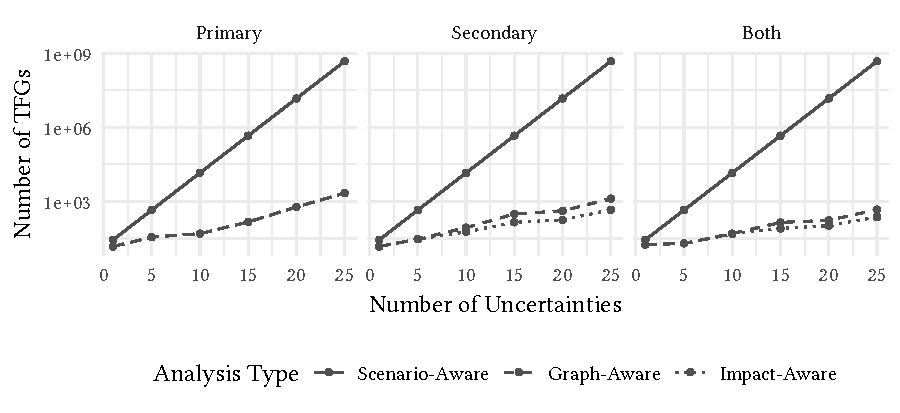
\includegraphics[width=\textwidth]{figures/chapter9/plot-CWA.pdf}
  \caption{Scalability results of the CoronaWarnApp evaluation scenario. Lower is better.}
  \label{fig:evaluation:result:g7:cwa}
\end{figure}

\begin{figure}
  \centering
  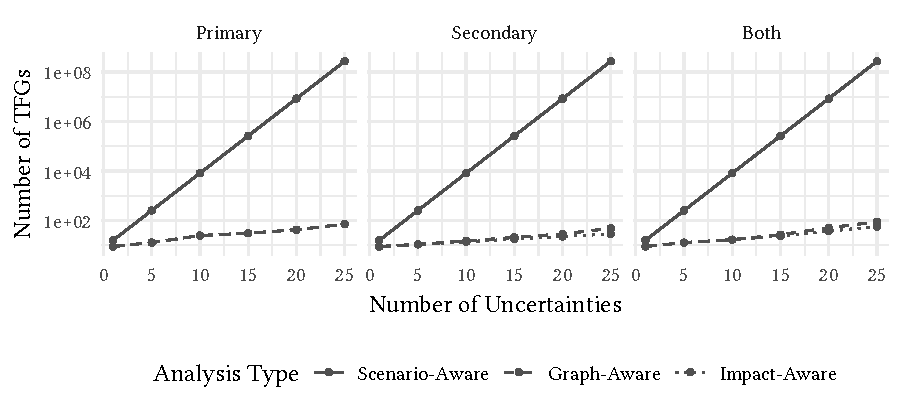
\includegraphics[width=\textwidth]{figures/chapter9/plot-MAAS.pdf}
  \caption{Scalability results of the MobilityAsAService evaluation scenario. Lower is better.}
  \label{fig:evaluation:result:g7:maas}
\end{figure}

Regarding the scalability of \emph{scenario-aware} analysis (\metric{7}{1}{1}), the results show the combinatorial explosion already discussed in the context of design space exploration \cite{koziolek_automated_2011}.
We also discussed this issue when introducing the different approaches to uncertainty-aware data flow analysis in \autoref{ch:confidentialityanalysis}.
For every uncertainty source---and every scenario of every source---the scenario-aware analysis calculates the combination of all possible scenarios, i.e., the Cartesian product.
Afterward, all \acp{TFG} need to be analyzed for every combination.
Especially in larger software systems with many data flows, this rapidly increases the run time.
However, also smaller systems are affected: The \emph{MobilityAsAService} scenario only has 8 \acp{TFG} compared to the 14 \acp{TFG} of the \emph{CoronaWarnApp}.
Still, for all 25 uncertainty sources, the analysis requires approximately 270 million \acp{TFG} compared to 470 million \acp{TFG}.
Both numbers are high enough to make the data flow analysis framework unsuitable \cite{schwickerath_tool-supported_2023}.
Regarding the scalability of \emph{graph-aware} analysis (\metric{7}{1}{2}), the number of required \acp{TFG} is highly reduced.
Using the information about depended uncertainties in the same \ac{TFG} and independent uncertainties in other \acp{TFG}, the majority of scenario combinations can be safely rejected.
This effect becomes visible in all non-trivial software systems that comprise more than a single \ac{TFG}.
Here, our measurements imply that the 8 \ac{TFG} of \emph{MobilityAsAService} are sufficient for a highly reduced complexity.
Regarding the scalability of \emph{impact-aware} analysis (\metric{7}{1}{3}), we see its relation to the occurrence of \emph{primary} and \emph{secondary} uncertainty.
The impact-aware analysis is able to consider the uncertainty interaction between \emph{secondary} and \emph{primary} uncertainty, as introduced in \autoref{sec:confidentialityanalysis:representing}.
Thus, the number of \acp{TFG} is not reduced when only including \emph{primary} uncertainty.
Although the reduction when including \emph{secondary} uncertainty is not as large compared to scenario-aware analysis, it is still notable.
On average, impact-aware analysis requires only $\frac{5.50}{7.09} = 0.78$ times as many \acp{TFG} for the same result in the evaluated scenarios.
Here, the results also indicate that the reduction correlates to the number of \acp{TFG} of the scenario.
We conclude that the results are satisfying regarding the \emph{scalability} comparison (\question{7}{1}) of uncertainty-aware data flow analyses.
Thus, we are able to define \emph{scalable} analyses (\goal{7}).
The results also empirically support the complexity reduction of more advanced uncertainty-aware data flow analysis, i.e., $N_{I} \leq N_{G} \leq N_{S}$, see \autoref{sec:confidentialityanalysis:complexity}.


\subsection{Results and Discussion of the Accuracy}

\begin{table}
  \centering
  \begin{tabular}{llr}
    \toprule
    Question & Metric & Result \\
    \midrule
    Structural uncertainty (\question{8}{1}) & Precision (\metric{8}{1}{1}) & $1.00$ \\
    & Recall (\metric{8}{1}{2}) & $1.00$ \\
    Environmental uncertainty (\question{8}{2}) & Precision (\metric{8}{2}{1}) & $1.00$ \\
    & Recall (\metric{8}{2}{2}) & $1.00$ \\
    Tracing uncertainty (\question{8}{3}) & Precision (\metric{8}{3}{1}) & $1.00$ \\
    & Recall (\metric{8}{3}{2}) & $1.00$ \\
    Impact-aware analysis (\question{8}{4}) & Precision (\metric{8}{4}{1}) & $1.00$ \\
    & Recall (\metric{8}{4}{2}) & $1.00$ \\
    \bottomrule
  \end{tabular}
  \caption{Results of evaluation Goal \goal{8} regarding the uncertainty-aware data flow analyses' accuracy.}%
  \label{table:evaluation:result:g8}
\end{table}

The eighth and last Goal \goal{8} focuses on the accuracy of the four approaches to uncertainty-aware confidentiality analysis, presented in \autoref{ch:confidentialityanalysis}.
This goal comprises four evaluation questions with a total of eight metrics.
\autoref{table:evaluation:result:g8} shows the results.
In the following, we first present these results and discuss them afterward.

The \emph{accuracy} of the data flow analysis under structural uncertainty (\question{8}{1}) asks about the \emph{precision} (\metric{8}{1}{1}) and \emph{recall} (\metric{8}{1}{2}) of the first analysis approach, introduced in \autoref{sec:confidentialityanalysis:structural}.
As discussed previously, we use the evaluation scenarios \emph{TravelPlanner}, \emph{DistanceTracker}, and \emph{OnlineShop} together with PerOpteryx \cite{koziolek_peropteryx_2011,koziolek_automated_2011}.
Although the introducing of the confidentiality analysis requires PerOpteryx to analyze many architectural candidates, see \autoref{sec:confidentialityanalysis:structural}, all candidates with confidentiality violations and also all candidates without violations were correctly identified.
This results in a perfect score of 1.0, both regarding precision and recall.
The \emph{accuracy} of the data flow analysis under environmental uncertainty (\question{8}{2}) asks about the \emph{precision} (\metric{8}{2}{1}) and \emph{recall} (\metric{8}{2}{2}) of the second analysis approach, introduced in \autoref{sec:confidentialityanalysis:environmental}.
Here, we use the evaluation scenarios \emph{TravelPlanner} and \emph{DistanceTracker}.
The introduction of uncertainty in \ac{RBAC} produces the expected confidentiality violations, i.e., the perfect scores of 1.0 for precision and recall.
The \emph{accuracy} of the approach to trace uncertainty in data flows (\question{8}{3}) asks about the \emph{precision} (\metric{8}{3}{1}) and \emph{recall} (\metric{8}{3}{2}) of the third analysis approach, introduced in \autoref{sec:confidentialityanalysis:tracing}.
The introduction of uncertainty as variation points in the variation creation \cite{mehl_palladio_2022} of the evaluation scenarios \emph{TravelPlanner}, \emph{DistanceTracker}, and \emph{OnlineShop}, produces variants of the software architecture, which partially violate confidentiality.
The analysis is able to correctly identify these variations and traces identified confidentiality violations back to the originating uncertainty sources.
Thus, it reaches both a precision and recall of 1.0.
Last, the \emph{accuracy} of the uncertainty-impact aware data flow analysis (\question{8}{4}) asks about the \emph{precision} (\metric{8}{4}{1}) and \emph{recall} (\metric{8}{4}{2}) of the fourth analysis approach, introduced in \autoref{sec:confidentialityanalysis:abunai}.
Here, we directly model the uncertainty sources as a first-class concern of all six evaluation scenarios, i.e., \emph{TravelPlanner}, \emph{DistanceTracker}, \emph{OnlineShop}, \emph{CoronaWarnApp}, \emph{MobilityAsAService}, \emph{JPlag}.
As discussed previously, we provide the most comprehensive accuracy evaluation for this approach as it represents our most advanced analysis.
In total, we identified 221 confidentiality violations due to uncertainty, which resulted in a precision of 1.0 and a recall of 1.0.

All four evaluation questions of Goal \goal{8} use the same metrics, i.e., \emph{precision} and \emph{recall}.
Moreover, all measurements show the perfect result of 1.0, both regarding precision and recall.
For the sake of simplicity, we jointly discuss all results instead of repeating the interpretation for all four questions (\question{8}{1} -- \question{8}{4}).
All presented uncertainty-aware data flow analysis approaches are based on the data flow analysis framework \cite{boltz_extensible_2024}, presented in \autoref{sec:confidentialityanalysis:framework}.
The framework itself follows the data flow analysis concept of \textcite{seifermann_architectural_2022} and shows equal results regarding identified confidentiality violations \cite{schwickerath_tool-supported_2023}, i.e., a precision and recall of 1.0.
The accuracy evaluation of \textcite{seifermann_architectural_2022}, which partially uses the same evaluation scenarios as used in our evaluation, results in a perfect accuracy of 1.0.
Put simply, to validate the accuracy of our analysis approaches, it is sufficient to show that we did not impair the analysis quality by introducing uncertainty into the modeling and analysis procedure.
The consistent results of 1.0 for both precision and recall support this.
Note that this does not resemble real-world accuracy measurements using case studies, as discussed in \autoref{ch:evaluationscenarios}.
Related work uses similar approaches to accuracy evaluation showing perfect results \cite{walter_context-based_2023,walter_architecture-based_2023,walter_architectural_2022-1,seifermann_detecting_2022,seifermann_data-driven_2019,boltz_modeling_2024}.
We conclude that the results are satisfying regarding the \emph{accuracy} of data flow analyses under structural uncertainty (\question{8}{1}) and environmental uncertainty (\question{8}{2}), and also regarding tracing uncertainty (\question{8}{3}) and the uncertainty-impact aware analysis (\question{8}{4}).
Thus, our approaches to uncertainty-aware data flow analysis are \emph{accurate} (\goal{8}).


\subsection{Threats to Validity}

We conclude the evaluation of the third Contribution \C{3} with a discussion of the threats to validity of Goal \goal{7} and \goal{8}.
Similarly to the previous evaluation, we use evaluation scenarios, described in \autoref{ch:evaluationscenarios}.
We follow the guidelines of \textcite{runeson_guidelines_2009}, who propose to discuss internal validity, external validity, construct validity, and reliability.
This addresses the lack of guidelines in threats to validity discussions \cite{konersmann_evaluation_2022}.


\paragraph*{Internal validity}
The internal validity reflects whether the evaluation results depend only on the factors examined, without being influenced by other factors.
Regarding Goal \goal{7}, the location of the injected uncertainty sources could influence the measured scalability results.
However, especially for the larger measurements, we argue that using randomly chosen locations is sufficient.
Additionally, the identified effect size is large, with speedups by orders of magnitude.
Although we cannot eliminate this risk, we find its impact negligible.
Regarding Goal \goal{8}, the biggest threat is the manual creation of the reference output, i.e., the gold standard of the evaluation scenarios.
We apply several strategies to mitigate this threat.
First, we use a mixture of evaluation scenarios from other work \cite{seifermann_detecting_2022,seifermann_architectural_2022,katkalov_model-driven_2013,katkalov_modellgetriebener_2017,seifermann_data-driven_2019,rausch_common_2008}, e.g., \emph{TravelPlanner} and \emph{DistanceTracker}, and self-defined evaluation scenarios based on real-world software systems, e.g., \emph{CoronaWarnApp} \cite{robert_koch_institute_open-source_2020}, and \emph{Jplag} \cite{prechelt_finding_2002,saglam_jplag_2024}.
Second, we use publicly available documentation to ensure the validity of confidentiality violations and sources of uncertainty.
Third, we continuously use the data flow analysis framework without considering uncertainty to validate identified confidentiality violations.
Fourth, the simpler scenarios are small enough to manually validate identified results.
Another threat to internal validity is the extension of PerOpteryx \cite{koziolek_peropteryx_2011} using the confidentiality analysis \cite{walter_architectural_2022}, which could impact the design space exploration algorithm.
We address this by only using the dedicated extension mechanism of PerOpteryx \cite{koziolek_automated_2011}.


\paragraph*{External validity}
The external validity reflects the generalizability of the evaluation results to other cases or domains.
Regarding Goal \goal{7}, we only consider the biggest evaluation scenarios \emph{CoronaWarnApp} and \emph{MobilityAsAService}.
We argue that this is sufficient, especially in large scenarios where combinatorial explosion can easily lead to scalability problems.
Thus, the sufficient scalability of graph-aware and impact-aware analysis should also apply to simpler scenarios.
Similarly to the evaluation of Contribution \C{2}, the biggest threat for Goal \goal{8} is the selection of evaluation scenarios.
We address this by ensuring a good mixture of minimal examples, e.g., \emph{TravelPlanner} or \emph{DistanceTracker}, and comprehensive scenarios, e.g., \emph{CoronaWarnApp} and \emph{MobilityAsAService}.
All scenarios show different numbers regarding the size of the architectural model, the extracted \acp{DFD}, modeled uncertainty sources and identified confidentiality violations.
Furthermore, they originate from different existing work and existing software systems from a multitude of domains, i.e., mobility, health, sports, e-commerce, and plagiarism detection.
They comprise all five uncertainty types, introduced in \autoref{sec:classification:classification}.
Similarly to the previous evaluation, we argue that the quality of uncertainty-aware data flow analysis does not depend on the domain and only relates to \acp{DFD} and considered uncertainty sources.


\paragraph*{Construct validity}
The construct validity reflects whether the measurements are suitable for representing the evaluation objectives.
Similarly to the previously presented evaluation of Contributions \C{1} and \C{2}, we apply a \ac{GQM}-based evaluation plan \cite{basili_methodology_1984,basili_goal_1994}.
Regarding Goal \goal{7}, the metrics for scalability depend on the complexity calculation, introduced in \autoref{sec:confidentialityanalysis:complexity}.
We argue that using these formulas is a valid approach as they directly represent the analysis algorithms presented in \autoref{ch:confidentialityanalysis}.
However, we do not provide formal proof but empirically evaluate the complexity using the evaluation scenarios.
We also do not collect runtime information as a previous study already indicated a high correlation between the number of \acp{TFG} and the analysis execution time.
We argue that measuring the required number of \acp{TFG} to consider uncertainty using the evaluation scenarios is sufficient.
Nevertheless, the applied metrics are not suitable for external comparisons as they lack normalization.
We only focus on the comparison of the scalability results of our analysis approaches.
Regarding Goal \goal{8}, we use precision and recall to measure accuracy.
Both represent well-known metrics of binary classification \cite{powers_evaluation_2011,van_rijsbergen_information_1979} that are commonly used to evaluate accuracy in software architectural research \cite{konersmann_evaluation_2022}.


\paragraph*{Reliability}
The reliability reflects the repeatability and whether the evaluation results are dependent on the specific researchers.
In contrast to the previous parts of the evaluation, the reliability of the results of Goal \goal{7} and \goal{8} is not threatened by the fact that the evaluation is only performed by a single researcher.
Here, all measurements were fully automated using the provided tooling, i.e., \uia and \abunai.
Nevertheless, to increase repeatability, we provide all modeled uncertainties, all raw evaluation data, the prototypical implementation, and all calculations as part of our data set \cite{dataset}.






\section{Summary and Outlook}%
\label{sec:evaluation:summary}

\begin{table}
  \centering
  \begin{tabular}{lllr}
    \toprule
    Goal & Question & Metric & Result \\
    \midrule
    \goal{1} & Generality (\question{1}{1}) & Laconicity (\metric{1}{1}{1}) & $0.95$ \\
    & & Lucidity (\metric{1}{1}{2}) & $0.70$ \\
    & Appropriateness (\question{1}{2}) & Completeness (\metric{1}{2}{1}) & $0.97$ \\
    & & Soundness (\metric{1}{2}{2}) & $1.00$ \\
    & Orthogonality (\question{1}{3}) & Orthogonality (\metric{1}{3}{1}) & $0.99$ \\

    \goal{2} & Reliability (\question{2}{1}) & Annotator consensus (\metric{2}{1}{1}) & $0.69$ \\
        & Correctness (\question{2}{2}) & Recall (\metric{2}{2}{1}) & $0.73$ \\
        & Ease of use (\question{2}{3}) & \ac{SUS} (\metric{2}{3}{1}) & $68.25$ \\

    \goal{3} & Relevance (\question{3}{1}) & Fraction of relevant classes (\metric{3}{1}{1}) & $1.00$ \\
        & Novelty (\question{3}{2}) & Innovation (\metric{3}{2}{1}) & $0.49$ \\
        & & Adaptation (\metric{3}{2}{2}) & $0.51$ \\
        & Significance (\question{3}{3}) & Classification delta (\metric{3}{3}{1}) & $0.54$ \\

    \goal{4} & Identification (\question{4}{1}) & Correctness (\metric{4}{1}{1}) & $0.88$ \\
        & Collaboration (\question{4}{2}) & Correctness (\metric{4}{2}{1}) & $0.65$ \\
        & Ease of use (\question{4}{3}) & \ac{SUS} (\metric{4}{3}{1}) & $69.71$ \\
        & & Average rating (\metric{4}{3}{2}) & $3.1 / 4$ \\

    \goal{5} & Accuracy (\question{5}{1}) & Precision (\metric{5}{1}{1}) & $0.78$ \\
        & & Recall (\metric{5}{1}{2}) & $1.000$ \\
        & & F\textsubscript{1} score (\metric{5}{1}{3}) & $0.88$ \\

    \goal{6} & Effort reduction (\question{6}{1}) & $ratio_{actual}$ (\metric{6}{1}{1}) & $0.11$ \\
        & & $ratio_{impact}$ (\metric{6}{1}{2}) & $0.14$ \\

    \goal{7} & Scalability (\question{7}{1}) & Scenario-aware (\metric{7}{1}{1}) & $\num{2.56e+06}$ \\
        & & Graph-aware (\metric{7}{1}{2}) & $7.09$ \\
        & & Impact-aware (\metric{7}{1}{3}) & $5.50$ \\

    \goal{8} & Structural (\question{8}{1}) & Precision (\metric{8}{1}{1}) & $1.00$ \\
        & & Recall (\metric{8}{1}{2}) & $1.00$ \\
        & Environmental (\question{8}{2}) & Precision (\metric{8}{2}{1}) & $1.00$ \\
        & & Recall (\metric{8}{2}{2}) & $1.00$ \\
        & Tracing (\question{8}{3}) & Precision (\metric{8}{3}{1}) & $1.00$ \\
        & & Recall (\metric{8}{3}{2}) & $1.00$ \\
        & Impact-aware (\question{8}{4}) & Precision (\metric{8}{4}{1}) & $1.00$ \\
        & & Recall (\metric{8}{4}{2}) & $1.00$ \\
    \bottomrule
  \end{tabular}
  \caption[Joint results of all evaluation goals, showing all questions, metrics, and results.]{Joint results of all evaluation goals, showing all questions, metrics, and results. This includes the evaluation Goals of structure's suitability (\goal{1}), applicability (\goal{2}), purpose (\goal{3}), usability (\goal{4}), accuracy (\goal{5}), effort reduction (\goal{6}), scalability (\goal{7}), and accuracy (\goal{8}).}%
  \label{table:evaluation:result:summary}
\end{table}

In this chapter, we presented the evaluation of all three Contributions \C{1}, \C{2}, and \C{3}.
First, we introduced a comprehensive \ac{GQM}-plan comprising 8 goals, 19 questions, and 32 metrics.
Afterward, we explained the evaluation design, and presented and interpreted the evaluation results separately for each contribution.
\autoref{table:evaluation:result:summary} shows an overview of all metrics, thereby combining the individually presented results of all Goals \goal{1} -- \goal{8}.
In the following, we summarize the results and also present key findings of the evaluation.

Our first Contribution \C{1} comprises a classification of uncertainty regarding confidentiality and a catalog of uncertainty sources.
We evaluated the classification structure's suitability (\goal{1}), its applicability (\goal{2}), and justified its purpose (\goal{3}), following the evaluation method of \textcite{kaplan_introducing_2022}.
Additionally, we evaluated the usability (\goal{4}) of our catalog.
With the classification, we enable a more precise description of uncertainty with regard to confidentiality.
With the tool-supported catalog approach \arcen, we intended to enhance the usability of the classification and also to address the \ac{UAP}.
The results of the evaluation indicate that both the classification and the catalog reach these goals.
With the classification, we provide common terminology that fits the required abstraction, e.g., with a high laconicity (\metric{1}{1}{1}) of 95\%, or a clearly positive classification delta (\metric{3}{3}{1}) of 0.54, and that is usable to name and describe uncertainty sources with regard to confidentiality, as seen with a recall (\metric{2}{2}{1}) of 73\%.
The catalog further supports the identification and description of uncertainty in architectural models with a correctness (\metric{4}{1}{1}) of 88\%.
Both are usable, as seen with a \ac{SUS} (\metric{2}{3}{1}) of $68.25 / 100$, or an average rating (\metric{4}{3}{2}) of $3.1 / 4$.
Based on the qualitative feedback of the participants of the two conducted user studies, combining both is expedient.
We find:

\finding{Both the uncertainty classification and the catalog of uncertainty sources support software architects in identifying, describing, and understanding software-architectural uncertainty with regard to confidentiality. 
However, combining both represents the most promising approach.}

Our second Contribution \C{2} is an architecture-based uncertainty impact analysis to predict confidentiality violations.
We evaluated the accuracy (\goal{5}) and effort reduction (\goal{6}) of the impact analysis compared to manual confidentiality analysis.
With the impact analysis tool-supported with \uia, we aim to accurately predict confidentiality violations with only a little overestimation but without any underestimation.
Furthermore, we want to support software architects by directing their attention to problematic parts of the software system and thereby reducing the required effort.
The evaluation results indicate that we have reached both goals.
The analysis reaches the perfect recall (\metric{5}{1}{2}) of 100\% while maintaining a precision (\metric{5}{1}{1}) of 78\%.
The required manual effort is highly reduced (\metric{6}{1}{2}), as software architects only need to consider 14\% of \ac{DFD} nodes on average, which is close to the optimal actual impact set ratio (\metric{6}{1}{1}) of 11\%.
In sum, we find:

\finding{The uncertainty impact analysis accurately predicts confidentiality violations due to uncertainty with only little overestimation.
Although the evaluation scenarios intentionally contained a multitude of confidentiality violations, only every tenth \ac{DFD} node was affected. 
This underlines the challenge of identifying confidentiality violations and the need for tool-supported analyses.}

Our third Contribution \C{3} comprises four approaches to uncertainty-aware data flow analysis to identify confidentiality violations due to uncertainty.
We evaluated the scalability (\goal{7}) of the three central awareness levels of uncertainty in data flow analysis, and the accuracy (\goal{8}) of our four analysis approaches.
Our goal is to identify all confidentiality violations due to uncertainty while maintaining reasonable scalability.
The evaluation results indicate that this is not trivial.
Our first approach, scenario-aware data flow analysis (\metric{7}{1}{1}), requires on average 2.5 million additional \acp{TFG} per uncertainty in our evaluation with 1 to 25 randomly injected uncertainty sources.
This severe lack of scalability is discussed as the combinatorial explosion in the context of design space exploration \cite{koziolek_automated_2011}.
However, both the graph-aware (\metric{7}{1}{2}) and the impact-aware (\metric{7}{1}{3}) data flow analysis requires significantly less \acp{TFG} per uncertainty source, averaging at 7.09, and 5.50, respectively.
All four analysis approaches reach the perfect precision and recall, as expected due to the testing conditions.
In sum, we find:

\finding{The four uncertainty-aware data flow analysis approaches accurately identify confidentiality violations due to uncertainty.
However, only graph-aware and impact-aware analyses are applicable due to the severe lack of scalability of uncertainty scenario-aware data flow analysis.
This underlines the need to provide scalable analysis approaches tailored to confidentiality.}

Overall, we find the evaluation results satisfying.
Some measurements represent the perfect, or nearly perfect results.
Examples are the accuracy evaluation of uncertainty-aware data flow analysis (\goal{8}), the recall of uncertainty impact analysis (\goal{5}), or the structure's suitability (\goal{1}) and purpose (\goal{3}) of the classification.
Other metrics indicate room for improvement despite being acceptable.
For instance, the precision of uncertainty impact analysis \goal{5}, or the usability of the first Contribution \C{1} could be enhanced.
However, all contributions represent novel approaches to identifying, describing, and analyzing uncertainty with regard to confidentiality.
Thus, we find near-optimal and partially perfect results to be sufficient and leave further optimization to future work. 
We find:

\finding{The evaluation provides evidence regarding the sufficient quality of this dissertation's contributions.
This indicates that the classification of uncertainty, the catalog of uncertainty sources, the uncertainty impact analysis, and the uncertainty-aware data flow analyses support software architects in the architecture-based inspection and assessment of confidentiality under uncertainty.}

This chapter comprises the evaluation of all three contributions, which were presented in the last three chapters. 
The first contribution is introduced in \readingpath{ch:classification}.
The second contribution is shown in \readingpath{ch:impactanalysis}.
The third contribution is presented in \readingpath{ch:confidentialityanalysis}.
An overview of the interplay of all contributions can be found in \readingpath{ch:overview}.





\section{In Simpler Words}%
\label{sec:evaluation:simple}

This thesis has three contributions.
First, a classification and catalog approach of uncertainty sources, which help software architects identify and understand uncertainty sources.
Second, an uncertainty impact analysis predicts potential confidentiality violations under uncertainty.
Third, uncertainty-aware data flow analyses that identify confidentiality violations due to uncertainty.
All contributions are meant to enlarge our current knowledge about the relationship between uncertainty and confidentiality and also to support software architects.
In this chapter, we conduct a comprehensive evaluation to investigate whether the contributions represent an enhancement compared to the state of the art.

In an evaluation of this size, many things can go wrong.
One common mistake is the collection of meaningless data to validate the contributions.
To counteract this, we use a so-called \acf{GQM}-plan.
Here, goals represent the qualities, we want to show, e.g., that our analysis is accurate and usable.
To investigate these goals, we answer evaluation questions, e.g., whether users were happy with our approach.
Metrics quantify the answers, e.g., by counting how many users correctly describe uncertainty sources using our classification.
In total, our evaluation has 8 goals, 19 questions, and 32 metrics.
To gather the required data, we conducted two user studies, in which real software architects, researchers, and students used our contributions.
Additionally, we use the evaluation scenarios, presented in the previous chapter.

It is very important that an evaluation is comprehensible for other researchers.
Thus, this chapter describes in detail how the evaluation is designed, how the studies were conducted, and how the results were calculated.
Here, we distinguish between the objective measurements and our subjective interpretation of the measurements.
We also discuss potential threats to validity, i.e., what could have gone wrong during the evaluation and to which extent this affects the trustworthiness of our results.
Last, we provide a data set \cite{dataset} that contains all raw data, and all implementations and calculations.
This enables other researchers to review our results or repeat the evaluation themselves.

Overall, the results of our evaluation are satisfying.
They are not perfect---but they are good enough for us to believe that we created something that actually surpasses the state of the art.
The evaluation provides evidence that our classification helps to better understand and describe uncertainty and that our catalog approach complements this very nicely.
We also find that the uncertainty impact analysis does not miss confidentiality violations when predicting an uncertainty source's impact.
However, it could be a little more precise, as it also yields incorrect confidentiality violations.
Still, such overestimation is common among such analyses.
Last, we see an excellent accuracy of our uncertainty-aware data flow analyses.
All analysis approaches correctly identify all confidentiality violations due to uncertainty.
We also see how important the scalability of an analysis is.
Only our more advanced analysis approaches scale well enough for a higher degree of uncertainty within a software system.
This so-called combinatorial explosion is a common problem of design space exploration analyses.
Our evaluation indicates that our proposed solutions work very well regarding confidentiality.
In sum, we are happy with these results---they took us a total of four years to collect.


\part{Epilog}
\chapter{Related Work}%
\label{ch:relatedwork}%
 

In this chapter, we present other work that is related to our contributions\footnote{We are well aware of the advances of generative artificial intelligence in summarizing research articles. Therefore, we assume that handwritten sections on related work---such as this one---could soon become obsolete. Thus, we focus on providing an understandable overview.}.
As the title of this thesis implies, our contributions revolve around three central topics: Uncertainty, software architecture, and confidentiality.
These topics represent the foundations of our work, presented in \autoref{ch:foundations}.
Related work exists in all intersections of these topics.
Thus, we structure related work by iteratively investigating work in these areas.

The remainder of this chapter is structured as follows:
We summarize work from the software engineering and software architecture research community that also addresses uncertainty.
Then, we focus on architecture-based approaches to security and confidentiality.
Last, we investigate uncertainty-aware approaches to confidentiality that do not require architectural abstraction.
This dissertation is at the center of these areas, combining aspects of confidentiality, software architecture, and uncertainty-related research.

\ownpublications{
\fancycite{hahner_dealing_2021}, 
\fancycite{hahner_architectural_2021}, 
\fancycite{boltz_handling_2022},
\fancycite{walter_architectural_2022},\linebreak
\fancycite{hahner_classification_2023},
\fancycite{hahner_model-based_2023},
\fancycite{hahner_architecture-based_2023}, 
\fancycite{camara_uncertainty_2024},
\fancycite{boltz_extensible_2024},
\fancycite{hahner_arcn_2024}
}





\section{Uncertainty and Software Architecture}%
\label{sec:relatedwork:uncertaintyXarchitecture}

The intersection of research on uncertainty and software architecture represents the largest field investigated in this chapter.
This is no surprise, as also the vast majority of our publications were presented at conferences and workshops that belong to these research communities.
Furthermore, uncertainty is often discussed using model-based approaches common in software architectural research \cite{troya_uncertainty_2021,sobhy_evaluation_2021}.
We start by giving an overview of surveys and research roadmaps of both communities.
Afterward, we briefly summarize publications on uncertainty taxonomies and approaches related to \acfp{SAS}.
Then, we summarize the comprehensive work that has been conducted to optimize software architectures or to use architectural knowledge in uncertainty-aware analysis.
Another relation of both areas are design decisions, as already discussed with the \emph{cone of uncertainty} \cite{mcconnell_software_1998}, see \autoref{sec:foundations:uncertainty}.
Last, we summarize work that focusses on uncertainty management and sharing architectural knowledge.


\subsection{Surveys and Research Roadmaps}

Recently, two large surveys were conducted within the \acf{SAS} community that are related to our work.
\textcite{troya_uncertainty_2021} conducted a \acf{SLR} and the modeling of uncertainty.
They investigate 123 primary studies to better understand the notions and formalisms used to represent uncertainty.
Furthermore, they discuss when uncertainty is analyzed and whether such analysis is tool-supported.
They present a comprehensive collection of formalisms used to represent uncertainty, e.g., variability models, fuzzy logic, or temporal logic.
Their results indicate a lack of analysis approaches that are able to handle heterogeneous uncertainty types, such as presented in \autoref{sec:impactanalysis:ufd}.
They also highlight the need for consolidated modeling solutions, as currently driven with the \acf{OMG} \acf{PSUM} \cite{PSUM} standard.
Furthermore, they mention the need of tool-supported processes, which we address with \abunai, \uia, and \arcen.
Regarding design time analyses like the one presented in this thesis, the most common approach are variability models, such as the uncertainty meta model presented in \autoref{sec:confidentialityanalysis:abunai}.
We conclude that our contributions use  techniques well-known from the state of the art, but surpass related work by providing comprehensive modeling support for heterogeneous uncertainty and tool-supported analyses.

\textcite{hezavehi_uncertainty_2021} present an overview of the research community based on questionnaires.
In two stages, they investigate uncertainty concepts, sources, methods, and challenges.
Their results motivate the design time analysis of uncertainty, which includes both uncertainty sources internal and external to the system under study.
They state that \enquote{only when enough knowledge is not available at design time, [\dots], uncertainty handling should be postponed to run-time} \cite{hezavehi_uncertainty_2021}.
Moreover, they find that the current state of the art lacks in including non-functional requirements both as optimization goal as well as side effects.
We address this shortcoming and the problem of dealing with concurrent sources of uncertainty in \autoref{ch:impactanalysis}
By providing a procedure to handle uncertainty in \autoref{sec:overview:procedure} and collecting uncertainty sources in \autoref{sec:classification:collaboration}, we also partially address the challenges of consolidating knowledge, providing guidelines, and dealing with unanticipated change.
Last, the authors present an initial reference process that shows many activities that are also contained in the procedure presented in \autoref{sec:overview:procedure}, e.g., uncertainty identification, modeling, and propagation.
\textcite{calinescu_understanding_2020} provide the findings of another survey in the \acp{SAS} community, focussed on understanding uncertainty.
They also highlight the challenges of dealing with unanticipated change and enhancing the explainability of \acp{SAS}.
With \arcen, we provide a step towards addressing these challenges in \autoref{sec:classification:identification}.
We conclude that our approach fits current research challenges.

Research roadmaps light current research directions and provide agendas and research challenges.
Here, \textcite{de_lemos_software_2013} describe a general roadmap regarding the research on \acp{SAS}.
They especially highlight the challenge of the design space's size.
We discussed this issue and how to address the combinatorial explosion regarding data flow analysis and confidentiality in \autoref{sec:confidentialityanalysis:complexity}.
To also at least partially tackle the identified challenge regarding processes, we describe a procedure with activities and roles in \autoref{sec:overview:procedure}.
More recently, \textcite{weyns_towards_2023} describe their findings on current challenges regarding uncertainty management.
They highlight the need for understanding uncertainty and providing end-to-end approaches.
We present a tailored classification in \autoref{sec:classification:classification}, and a procedure that starts at the identification of uncertainty in \autoref{ch:classification} and ends after analyzing issues due to uncertainty in \autoref{ch:confidentialityanalysis}.
Thereby, we address these challenges regarding confidentiality as a non-functional requirement.


\subsection{Uncertainty Taxonomies and Classifications}

To better understand uncertainty, researchers created several taxonomies \cite{bures_capturing_2020,esfahani_uncertainty_2013,mahdavi-hezavehi_classification_2017,perez-palacin_uncertainties_2014,ramirez_taxonomy_2012,walker_defining_2003,PSUM,camara_uncertainty_2017}.
\textcite{walker_defining_2003} present a taxonomy of uncertainty using three dimensions. 
The \emph{location} describes where the uncertainty can be found, e.g., in the model input or context. 
The \emph{nature} distinguishes between epistemic (i.e., lack of knowledge) and aleatory (i.e., natural variability) uncertainty. 
Last, the \emph{level} describes how much is known about the uncertain influence.
Although this taxonomy has been the baseline for many others, it does not specifically aim to describe software-related uncertainty.
\textcite{perez-palacin_uncertainties_2014} build on this classification in the context of \acp{SAS}. 
They thereby adjust the dimension \emph{location} to better fit software models.
\textcite{bures_capturing_2020} adapt this taxonomy again to \enquote{fit the needs of uncertainty in access control} \cite{bures_capturing_2020}.
Although this work only considers access control in Industry 4.0 scenarios, it is also a good foundation for our classification, presented in \autoref{sec:classification:classification}.
\textcite{esfahani_uncertainty_2013} describe characteristics of uncertainty and hereby focus on the variability and reducibility of different sources of uncertainty.
They highlight the problem of uncertainty in the environment of a software system, e.g., due to the deployment.
\textcite{mahdavi-hezavehi_classification_2017} propose a classification framework of uncertainty.
They aim at architecture-based, \acp{SAS} but do also not consider security, privacy, or confidentiality.
Also related is the uncertainty template by \textcite{ramirez_taxonomy_2012}.
They present a scheme to describe uncertainty sources for dynamically adaptive systems in requirements, design, and runtime.
Due to the different scope, they describe uncertainty in software architecture as \emph{inadequate design} which is not precise enough to identify the impact of software-architectural \cite{hahner_classification_2023} uncertainty on confidentiality.
Still, they also list \emph{unexplored alternatives} and \emph{misinformed trade-off analysis} which motivates our work.
\textcite{armour_five_2000} presents the order of ignorance which also influenced many of the aforementioned taxonomies, e.g., the work of \textcite{perez-palacin_uncertainties_2014}.

More recently, the \ac{OMG} \ac{PSUM} \cite{PSUM} standard represents a joint effort towards the standardization of terminology to describe uncertainty.
However, at the time of writing, this still represents a work in progress.
A more in-depth discussion of related classifications can be found in \autoref{sec:classification:investigating}.
There, we not only show in detail all existing dimensions but also where we adapt or innovate on the state of the art.
This question is also part of our third evaluation goal \goal{3}, presented in \autoref{sec:evaluation:first}.
We conclude that there has been a substantial effort in the last decades to classify uncertainty.
Based on the comprehensive findings of related work we present a novel classification tailored to confidentiality.
Revisiting related work underlines both the need for tailored classification systems and the appropriateness of our classification to confidentiality, see \autoref{sec:classification:investigating} and \autoref{sec:evaluation:first}.


\subsection{Architecting Self-Adaptive Systems}

As discussed in \autoref{sec:foundations:uncertainty} and in \autoref{sec:classification:relation}, uncertainty is central topic in the \acp{SAS} research community.
However, the software architectures considered in this thesis are not self-adaptive, and further research is required to understand the implications of our findings for such software systems completely.
Nevertheless, we briefly summarize related work in this field.

The \emph{Rainbow} framework by \textcite{garlan_rainbow_2004} enables architecture-based self-adaptation.
The architecture layer comprises an adaptation engine and logic for constraint evaluation to monitor the runtime system and to adapt in case of occurring issues, e.g., regarding the system performance.
As this evaluation is model-based, we argue that our approach could be integrated into this framework to simplify its use at runtime.
Proper modeling and analysis support---such as the one presented in this thesis---is required to identify confidentiality violations \cite{seifermann_architectural_2022,schneider_how_2024}.
In another publication, the authors present the \emph{Znn.com} system to evaluate the Rainbow framework.
We build on this software system to present our approach to addressing the \ac{UIP} in \autoref{sec:impactanalysis:ufd}.

\textcite{andersson_modeling_2009} present modeling dimensions of \acp{SAS}, i.e., variation points of said systems.
They distinguish four groups of dimensions: Goals, changes, mechanisms, and effects.
In the scope of this work and the already discussed uncertainty classifications, this can be seen as a more general description of the underlying challenges of \acp{SAS}.
Using our terminology, uncertainties causing changes have sources and types, as described in \autoref{sec:classification:relation}.
Here, our classification describes a small subset of these dimensions in more detail, justified by the purpose of conducting confidentiality analysis.
This underlines the relation of our work to \acp{SAS}, as already illustrated in recent publications \cite{weyns_towards_2023,camara_uncertainty_2024}.

\textcite{whittle_relax_2009} present \emph{RELAX}, an approach targeted at considering uncertainty in requirements engineering of \acp{SAS}.
By weakening requirements depending on the environmental conditions monitored during runtime, self-adaptation can be achieved in a structured manner.
The authors argue that, compared to ad-hoc approaches, considering uncertainty in requirements helps to describe clear adaptation boundaries and to ensure invariants.
However, this approach does not consider the development of the system nor provides mechanisms to satisfy the weakened requirements. 
In addition, it can only cope with environmental uncertainty that is known during formulating the requirements.
Nevertheless, we argue that revisiting confidentiality requirements under uncertainty represents a promising research direction for future work.


\subsection{Architecture Evaluation Under Uncertainty}

The topic of architecture evaluation under uncertainty represents the most comprehensive section of related work.
Numerous approaches \cite{esfahani_dealing_2012,koziolek_peropteryx_2011,aleti_archeopterix_2009,lytra_supporting_2013,vanherpen_design-space_2014,esfahani_guidearch_2013} have been proposed to evaluate and optimize software architectures.
They often refer to the variability or inherent uncertainty in software architecture as \emph{design space exploration}, which can also be described as \enquote{searching better or even optimal designs} \cite{koziolek_automated_2011}.
\textcite{sobhy_evaluation_2021} conducted a \ac{SLR} comprising 48 primary studies on this topic.
They highlight the focus on design time, which matches our approach.
We summarize the most related approaches.

\emph{PerOpteryx} \cite{koziolek_peropteryx_2011,martens_automatically_2010,koziolek_automated_2011} is a model-based approach to optimize software architectures regarding quality properties like performance, cost, or reliability.
\textcite{koziolek_peropteryx_2011} employ evolutionary optimization to find Pareto-optimal architectural candidates.
To assess the quality of the candidates, they use the Palladio approach, introduced in \autoref{sec:foundations:architecture}.
However, there is no support for confidentiality, although there is already a PerOpteryx extension for security \cite{busch_modelling_2016}.
In contrast to our approach, they modeled these by a concept of concerns. 
These concerns describe which design decisions are dependent on each other. 
In our analysis we focus on the direct impact on confidentiality.
Similarly to the relation to Rainbow \cite{garlan_rainbow_2004}, we argue that our approach can be incorporated or combined with PerOpteryx.
We demonstrated this while defining a scenario-aware data flow analysis regarding structural uncertainty in \autoref{sec:confidentialityanalysis:typespecifc}.

\textcite{esfahani_guidearch_2013} present \emph{GuideArch}, an approach to explore the architectural solution space under uncertainty. 
This shall enable software architects to identify critical design decisions.
They apply fuzzy math to represent uncertainty and its impact on the software architecture.
This enables the comparison of architectural candidates and the exploration of the solution space.
Although this approach considers uncertainty and fuzziness on the architectural abstraction level, it does not consider confidentiality or other privacy-related quality properties.
By applying fuzzy methods in graph-aware data flow analysis, we found that their expressiveness is limited regarding confidentiality, which is hard to quantify, see \autoref{sec:confidentialityanalysis:typespecifc}.
Thus, we argue that the application of GuideArch to analyze confidentiality is not straightforward.

Another design space exploration tool is \emph{ArcheOpterix} by \textcite{aleti_archeopterix_2009}. 
It can also optimize a given architecture for multiple criteria using evolution techniques and design constraints.
However, similarly, it does not support a confidentiality analysis, and the design space modeling is more restrictive.
The quality attributes of \enquote{safety, reliability, security, performance, timeliness, and resource consumption} \cite{aleti_archeopterix_2009} are only considered to be future work for ArcheOpterix.
At the time of writing, we were unable to find analysis extensions suitable for security, privacy, or confidentiality.
\textcite{vanherpen_design-space_2014} also present an approach to model-based design space exploration.
They present a pattern catalog of techniques known from architecture optimization but do not focus on analysis support.
\textcite{gerasimou_synthesis_2018} present \emph{EvoChecker}, a search-based approach employing evolutionary algorithms in automated model synthesis.
They focus on quality of service properties like reliability, response time, and cost.
In sum, design space exploration approaches are versatile, but do often not support security-related attributes but focus, e.g., on performance.
While these approaches can analyze a wide variety of quality properties, they are not appropriate to consider confidentiality as they lack the required expressiveness to consider data processing and data flow constraints.

Last, there is a relation to the topics of variability, product lines, and testing, as they share similar challenges regarding the size of the design space and combinatorial explosion, as discussed in \autoref{sec:confidentialityanalysis:complexity}.
Here, \textcite{abbas_modeling_2012} propose to model the variability in quality concerns, thereby expressing what does vary how and for which reason.
This shall reduce the number of required quality attribute scenarios.
Another approach is the combination of design models and test models to minimize testing efforts while facing feature interaction and ensuring a comprehensive coverage of interactions.
\textcite{oster_pairwise_2011} combine pairwise feature generation with model-based testing and \textcite{lochau_model-based_2012} combine feature models and state charts that represent test models.
The challenge of feature interactions is comparable to dealing with uncertainty interactions, see \autoref{sec:impactanalysis:ufd}.
By employing the notion of independent \acfp{TFG}, we can minimize the required analysis effort due to interacting uncertainties, see \autoref{sec:confidentialityanalysis:framework}.
Here, mapping the uncertainty model to the architectural model to minimize the analysis effort is comparable to the mapping applied in related work.
We require full coverage of all interactions on a single \ac{TFG}, as a missing variation could cause missed confidentiality violations due to uncertainty, see the discussion of recall in \autoref{sec:evaluation:overview}.


\subsection{Architecture-Based Analysis}

Besides automatically optimizing software architectures proposed in the previous paragraphs, architectural models are often used as a means to analyze the quality of software architectures or to help in the design process.
These approaches are closely related to this thesis as we also build on the architectural model to analyze confidentiality.
In the following, we summarize related architecture-based analyses.

When considering architectural models as a baseline for uncertainty analysis, we first have to address the question of incorporating uncertainty into the model.
Here, \textcite{garlan_software_2010} proposed already more than a decade ago to consider uncertainty as a first-class entity.
There are numerous notations for incorporating uncertainties of different types into software models \cite{troya_uncertainty_2021}. 
For instance, SysML~\cite{object_management_group_omg_2023} and the \acf{UML} MARTE Profile~\cite{object_management_group_uml_2011} provide stereotypes and properties to represent some types of uncertainty, especially measurement uncertainty. 
However, existing notations allow modeling mostly homogeneous uncertainties, i.e., of the same type.
The aforementioned \ac{PSUM} standard \cite{PSUM} also provides a metamodel for representing different types of uncertainty but is still a work in progress.
Regarding measurement uncertainty, \textcite{bertoa_incorporating_2020} propose its inclusion into primitive data types of \ac{UML} models.
Our modeling approach of uncertainty and our distinction between five central uncertainty types is also inspired by the aforementioned work, see \autoref{sec:classification:investigating}.
As discussed in \autoref{sec:classification:classification} and \autoref{sec:confidentialityanalysis:typeagnostic}, we can express all identified uncertainty sources \cite{hahner_arcn_2024} as part of the architectural model.

\textcite{famelis_managing_2019} introduce \emph{DeTUM}, which stands for design time uncertainty management.
This tool-supported approach handles uncertainty using partial models.
It introduces uncertainty in the start phase and then resolves it in later stages.
They also refer to open design decisions as a source of uncertainty, similarly to the \emph{cone of uncertainty} \cite{mcconnell_software_1998}, see \autoref{sec:classification:relation}.
However, the authors do not mention security-related quality attributes like confidentiality.
They explicitly mention the requirement of external support to assess the impact of uncertainty---as we offer it with our work.

\textcite{goseva-popstojanova_assessing_2003} present an approach for architecture-based reliability analysis under uncertainty.
Here, values such as the probability that a particular component is used or the reliability of a component contribute to the analysis of uncertainty.
Using Monte Carlo simulation, the authors can analyze how uncertainty propagates from model parameters into reliability estimations.
Although we investigate another quality property and use data flow analysis instead Monte Carlo simulation, we argue that our method is comparable.
Both approaches use appropriate architectural models and derive the impact of uncertainty.
However, we argue that confidentiality and reliability as quality properties differ fundamentally.
Therefore, the approach is not suitable for detecting confidentiality breaches, and we are not able to analyze reliability.
In sum, there exist many approaches to model and analyze uncertainty regarding other quality properties of software architectures. 
However, they do not explicitly take confidentiality into account.


\subsection{Architectural Design Decisions and Uncertainty}
\acfp{ADD} are related to uncertainty.
As depicted with the \emph{cone of uncertainty} \cite{mcconnell_software_1998}, open design decisions introduce uncertainty about the software system to design, and making decisions reduces said uncertainty.

\textcite{kruchten_ontology_2004} presents an ontology of \acp{ADD}.
The author distinguishes between existence, property and executive decisions and provides an overview of \acp{ADD} attributes.
This is especially relevant when considering uncertainty that can void existing decisions and require software architects to backtrack.
\textcite{jansen_software_2005} see software architecture as a composition of \acp{ADD}.
This shows how uncertainty, e.g., about the system context, can hinder good software design as the \emph{best} decision might not be found.
Although both approaches do not focus on uncertainty, they inspired our classification which is strongly coupled to architectural design, see \autoref{sec:classification:classification}.

\textcite{lytra_supporting_2013} propose the use of fuzzy logic to incorporate inherent uncertainty into reusable \acp{ADD}.
This shall enable software architects to share and reuse knowledge about the impact of uncertainty on quality attributes.
They employ a \acf{FIS} to identify the most appropriate design decisions and also foster the importance of decision documentation.
This is related to our data flow analysis under environmental uncertainty that is also based on fuzzy inference, see \autoref{sec:confidentialityanalysis:typespecifc}.
Furthermore, we also address knowledge exchange and documentation with our uncertainty catalog, see \autoref{sec:classification:collaboration}.
Although this approach can also handle security-related quality attributes, violations due to integration issues remain hidden.
Here, the integration of a dedicated analysis---such as our confidentiality analysis---helps identifying also fine-grained problems.
Future work could investigate whether defining reusable \acp{ADD} to ensure confidentiality is feasible.

\textcite{zimmermann_reusable_2007} present a framework to support the identification, making, and enforcement of \acp{ADD}.
This is especially helpful regarding the aforementioned backtracking, i.e., reverting decisions in case of design errors.
Here, awareness of dependencies minimizes the required effort and the chance of introducing new errors while backtracking.
\textcite{noppen_jar_software_2008} discuss design decisions under imperfect information by explicitly modeling uncertain aspects of the architecture based on fuzzy techniques and design trees to record the design history.
\textcite{busari_radar_2017} present the \emph{RADAR} approach \cite{busari_modelling_2019} that comprises a modeling language and decision analysis support.
They highlight dependencies between decisions and provide support to find Pareto-optimal solutions.
Although these approaches help to minimize errors during the design and help to recall the decision paths, they do not support analyzing software systems regarding confidentiality.
Nevertheless, we argue that such frameworks are helpful in combination with modeling and analysis support, which should be investigated in the future.


\subsection{Uncertainty Management and Knowledge Sharing}

Regarding the management of uncertainty and \acp{ADD}, the previous paragraphs introduced a multitude of approaches for modeling, analyzing, and optimizing software architectures.
In the following, we focus on uncertainty management and knowledge sharing beyond the design of single software systems.
Collecting and consolidating knowledge on architectural design and uncertainty supports software architects \cite{weyns_towards_2023,lytra_supporting_2013,zimmermann_reusable_2007,gerdes_decision_2015}.
It can help to address unanticipated change that is not completely unforeseen and can be tackled, e.g., by minimizing assumptions or creating reusable system building blocks. \cite{garlan_unknown_2021}.
The need for uncertainty management, reusable methods, and end-to-end approaches has also been highlighted in the aforementioned surveys and research roadmaps \cite{weyns_towards_2023,weyns_introduction_2020,troya_uncertainty_2021,hezavehi_uncertainty_2021}.
Knowledge sharing to counter uncertainty is also known from legal sciences \cite{sterz_intelligente_2022}.

With \arcen, we present a catalog of uncertainty sources to overcome the limitation of knowledge being scattered among researchers and institutions.
A related approach is \emph{Decision Buddy}, a tool-supported collaborative approach regarding design decisions by \textcite{gerdes_decision_2015}.
By collecting and describing the effects of \acp{ADD}, the decision-making of software architects can be supported with suitable and ranked solutions.
\emph{privacypatterns.eu} is a web-based collection of patterns to enhance privacy \textcite{colesky_system_2018}.
The collection comprises patterns like access control, single point of contact, or informed consent \cite{colesky_system_2018-1}
Last, \emph{arc42} represents an interactive collection of software qualities \cite{starke_arc42_2024}, comprising requirements, definitions, and relations.
These works provide comparable approaches to our proposed solution but cannot be applied to uncertainty and confidentiality due to the domain gap.
Additionally, the aforementioned tooling is partially fragile due to link decay \cite{goh_link_2007} or lacks open accessible data.
To counter such issues and to reach high usability and longevity, our tool support is publicly available, see \autoref{sec:classification:collaboration}.
Ultimately, we want to stress the importance of efforts towards catalogs and guidelines, especially with regard to cooperation among researchers and science transfer\footnote{The importance of guidelines and checklists was already emphasized by practitioners at EMLS' 21, in the very first workshop in which our approach was discussed \cite{hahner_dealing_2021}. \arcen represents one result of these findings, which received very positive reviews and feedback from the community.}.

\textcite{jasser_reusing_2016} present a repository of security solutions to support \acp{ADD}.
Exemplary solutions are access control, input sanitization, or the principle of the least privilege.
Here, the focus on security as a central quality property enables more precise classification, e.g., by relating to sub-goals like confidentiality, integrity, or availability \cite{international_organization_for_standardization_isoiec_2018}.
We consider this to be highly related to our catalog approach, although we approach the challenge from the opposite direction: Instead of providing solution techniques, we focus on supporting the identification of potential problems in the form of uncertainties.

Last, \textcite{lupafya_framework_2022} present a framework for considering uncertainty in the software design.
Their conceptual model connects viewpoints to uncertainties, risks and opportunities, and their mitigation or exploitation.
Furthermore, they present a classification of uncertainty based on consolidating existing work.
Although the approach looks promising at first sight, it falls short of providing further management, modeling, or analysis support beyond describing uncertainty sources with attributes.
Furthermore, combining existing classifications without further purpose lacks novelty \cite{kaplan_introducing_2022}.


\subsection{Summary}

The intersection of research on software architecture and uncertainty presented in this section represents the largest body of related work.
According to the aforementioned surveys, the state of the art is still of an exploratory nature, lacks comprehensive tool support \cite{troya_uncertainty_2021,hezavehi_uncertainty_2021}, and does also not focus on confidentiality.
Our approach addresses this gap regarding confidentiality with ready-to-use tool support that can easily be incorporated into existing approaches.
Furthermore, related work often inspired us.
For instance, our classification is based on existing taxonomies but tailored to confidentiality.
The decision to opt for a web-based and open-source catalog approach was also influenced by the perceived link decay \cite{goh_link_2007} of related work.
Our approach is by far not the first to incorporate uncertainty modeling in the form of scenarios into the architectural design.
However, we were unable to find related work that can identify confidentiality violations due to uncertainty.
We conclude that our approach represents novel work that can be combined with existing frameworks to compose comprehensive end-to-end approaches \cite{weyns_introduction_2020}.

\finding{Related work provides the foundation and inspiration for many aspects of our research.
However, to the best of our knowledge, there exists no directly comparable approach.
Ultimately, combining multiple analyses that differ in supported uncertainty sources and targeted quality properties is expedient.}





\section{Software Architecture and Confidentiality}%
\label{sec:relatedwork:architectureXconfidentiality}

The next section of related work we discuss in this thesis represents the intersection of software architecture and confidentiality.
We present work from the field of model-based security analysis and existing approaches to architectural data flow analysis.
Afterward, we revisit the specification of confidentiality requirements as they represent one important input to data flow analysis that can impact the accuracy of identified confidentiality violations.
This includes related work on access control.


\subsection{Model-based Security Analysis}

Model-based analyses use the model representation of software systems to evaluate their quality, e.g., by using architectural models.
They use techniques known from \acf{MDSD}, see \autoref{sec:foundations:mds}.
\textcite{nguyen_extensive_2015} present a \ac{SLR} based on 108 primary studies.
They find that the vast majority of papers use standardized notations like the \ac{UML}, but only less than half of the investigated papers consider confidentiality.
When confidentiality is discussed, it is often combined with considering authentication or authorization.
Only 11\% of the investigated publications focus on analyzing confidentiality.
They also find a lack of analyses that simultaneously consider multiple security concerns.

\textcite{goos_umlsec_2002} present \emph{UMLsec} that extends \ac{UML} by defining a security profile \cite{juerjens_principles_2002,goos_towards_2001}. 
By incorporating security-related information into \ac{UML}, software architects can reuse existing \ac{UML} diagrams for security analysis.
It supports different kinds of analyses, such as information flow or access control. 
In contrast to our confidentiality analysis approaches, it does not support access control on data, or more complex confidentiality requirements that go beyond, for instance, encrypted communication.
Another \ac{UML} security profile is \emph{SecureUML} by \cite{lodderstedt_secureuml_2002}. 
It supports \acf{RBAC} together with statements in the \acf{OCL} to support dynamic properties in authorization constraints.
Similarly, there is no support for more advanced constraints regarding confidentiality.
Although both approaches represent relevant steps towards model-driven security, they both show the lack of comprehensive support for confidentiality beyond access control, or encryption, as already discussed in the aforementioned survey.
Furthermore, they do not support uncertainty in their analyses.
Last, \textcite{ronneberg_quantitative_2024} propose information flow analysis in \ac{CBSE}, following the approach of correctness-by-construction to enable security guarantees.

\textcite{walter_architectural_2022-1} present a comprehensive approach to identifying confidentiality violations using attacker propagation \cite{walter_architectural_2022-1,walter_architecture-based_2023} and attack path analysis \cite{walter_architecture-based_2023-1,walter_context-based_2023}.
They extend the \acf{PCM} \cite{reussner_modeling_2016} to express vulnerabilities and access control with the \acf{XACML} \cite{oasis_extensible_2013}.
This enables the propagation of attackers within the software architecture.
After each propagation step, the analysis considers which credentials or access rights the attacker might have obtained, e.g., due to vulnerabilities within the system.
The approach also considers dependencies within the software architecture.
For instance, if an attacker gains access to a resource container, this also affects all components deployed on this resource.
The resulting attack graphs shall help software architects to estimate the impact of vulnerabilities and access control decisions.
This approach is highly related to our work, as it uses a similar approach to architectural models \cite{reussner_modeling_2016} and architecture-based propagation \cite{hahner_architecture-based_2024,busch_architecture-based_2020}.
However, it has two limitations regarding our needs.
First, there is no consideration of data flows, as confidentiality violations are identified by tracing attack paths.
Second, there is no comprehensive support for considering uncertainty, although initial approaches exist \cite{walter_architecture-based_2023}.
The authors acknowledge this limitation and state that \enquote{the combination with other uncertainty mitigation approaches} \cite{walter_context-based_2023} could be expedient.


\subsection{Data Flow Analysis}

The concept of \acp{DFD} and data flow analysis is not new \cite{demarco_structure_1979}.
Nevertheless, data flow analysis approaches are often used to assess the security of software systems.
This can be achieved by building on noninterference like \emph{JOANA} \cite{snelting_checking_2014} or deductive verification like \emph{KeY} \cite{ahrendt_deductive_2016}.
Other approaches extract data flows from source code without considering the software architecture.
\emph{RogueOne} by \textcite{sofaer_rogueone_2024} uses data flows to identify rogue updates, i.e., malicious changes to widely used libraries that aim to attack dependent software systems.
More recently, GitHub \cite{github_codeql_2021} pushes the adoption of \emph{CodeQL} \cite{de_moor_ql_2008} for data flow-based source code analysis and vulnerability detection.
Due to the broad applicability, such analyses represent promising approaches to analyzing the confidentiality of real-world software.
However, they lack the connection to the architectural abstraction, which becomes visible, e.g., when considering architecture-related information like the deployment.
Here, approaches to connect source code analyses and architectural analyses exist, e.g., by \textcite{kramer_model-driven_2017} and \textcite{reiche_modeling_2021}.
However, they do not consider uncertainty.
Combining source code analyses with architectural analyses and making uncertainty-aware represents a promising direction for future research.
With appropriate tool support, \acp{DFD} represent a powerful and commonly used mechanism for threat analysis \cite{bernsmed_adopting_2022} that helps in identifying security-related issues \cite{schneider_how_2024}.

The most related architectural data flow analysis is presented by \textcite{seifermann_detecting_2022}.
Their approach considers additional context information, such as the deployment, enabling software architects to analyze confidentiality during early design phases. 
We introduced their underlying meta model for the confidentiality-focused analysis of \acp{DFD} in \autoref{sec:foundations:dfd}.
Furthermore, they present an approach for label propagation to identify confidentiality violations.
Software architects can specify and analyze confidentiality requirements regarding noninterference, encryption, or access control.
A \acf{DSL} \cite{hahner_modeling_2021,hahner_domain-specific_2020} enables the specification of data flow constraints.
Our data flow analysis framework \cite{boltz_extensible_2024}, introduced in \autoref{sec:confidentialityanalysis:framework}, builds on this approach. 
However, the original data flow analysis is unable to consider uncertainty.
The authors acknowledge this limitation and the importance of considering uncertainty in the architectural design and analysis \cite{seifermann_architectural_2022}.

\textcite{boltz_model-based_2022} focus on the collaboration of legal and software experts in the assessment of information security and data protection.
They propose a model-based approach using the data flow analysis framework \cite{boltz_extensible_2024} described in \autoref{sec:confidentialityanalysis:framework}.
By using the \acf{ADL} \ac{PCM}, analyses of multiple quality properties are also possible, e.g., regarding performance and security \cite{boltz_modeling_2024}.
However, their approach only considers uncertainty coming from the legal side.
Here, combining our findings on modeling and analyzing uncertainty could be a promising approach.
\textcite{pilipchuk_architectural_2021} present an access control analysis based on business processes to align processes and access control policies \cite{pilipchuk_aligning_2018}.
By extracting access control requirements from business processes and using them in architecture-based data flow analysis, forbidden data flows can be identified.
However, this approach also focuses on conformance without considering uncertainty.

\textcite{peldszus_secure_2019} also present a data flow analysis approach called \emph{SecDFD}.
They check for compliance between models of the design and the implementation to identify violations.
The mapping is automated but lacks support for custom analysis definitions or data flow constraints and also does not consider uncertainty.
The early detection of design flaws \cite{tuma_automating_2020,tuma_flaws_2019} is closely related to the aforementioned data flow analysis by \textcite{seifermann_detecting_2022} and was also a baseline for the unified modeling primitives for \acp{DFD} used in our work, see \autoref{sec:foundations:dfd}.
Another approach is \emph{iFlow} by \textcite{katkalov_model-driven_2013}.
They use \ac{UML} models to derive and analyze data flows.
Furthermore, the generated source code can be verified.
\textcite{gerking_model_2018} present a model-based information flow analysis to identify timing channels.
Both approaches do not consider uncertainty, but \textcite{gerking_model-driven_2020} mentions the incorporation of uncertainty as potential future work.

Last, \textcite{schneider_automatic_2023} present an automated approach to extract \acp{DFD} from the source code of microservice applications.
They enrich the extracted \acp{DFD} with security-related information, e.g., regarding data storage, passwords, or logging.
This enables comprehensive data flow analysis that also considers architectural information.
They also published a large data set comprising the \acp{DFD} of 17 real-world microservice systems \cite{schneider_microsecend_2023}.
In a proof of concept, we transformed and analyzed this data set using our data flow analysis framework \cite{boltz_extensible_2024} to replicate the identified confidentiality violations.
There are also other steps towards security benchmarks \cite{bambhore_tukaram_towards_2022}.
We state that this represents a promising first step towards comprehensive data flow analysis that considers both the information from the source code and the software architecture.
However, similar to the previously discussed approaches, uncertainty is not considered. 


\subsection{Modeling Confidentiality Requirements}

The data flow analysis approaches presented in this thesis use confidentiality requirements in the form of data flow constraints as input, see \autoref{sec:foundations:dfd}.
Similarly, many related approaches discussed in the previous paragraphs use a dedicated requirement specification language.
Often, confidentiality requirements are also specified using access control \cite{nguyen_extensive_2015}.
The specification of confidentiality requirements impacts the identified confidentiality violations, with our without considering uncertainty.
We briefly summarize related work in both fields in the following.

\textcite{onabajo_properties_2006} investigated the properties of confidentiality requirements using grounded theory.
They present a model for requirements comprising elements like data, stakeholders, statements, purpose, and temporal validity.
This shall support the precise definition of requirements and enable the formal reasoning on derived rules, e.g., from legal frameworks like the \acf{GDPR} \cite{council_of_european_union_regulation_2016}.
To provide a foundation to describe such confidentiality requirements for data flow analysis, we presented a meta model and a \ac{DSL} in previous work \cite{hahner_modeling_2021}.
Data flow constraints follow the pattern of disallowing flows under certain conditions based on the characteristics of the data and involved entities or parts of the system.
A generalized form of this \ac{DSL} was presented with the data flow analysis framework \cite{boltz_extensible_2024}.
However, these approaches are not able to express restrictions with regard to uncertainty, e.g., whether certain flows shall not be allowed under given uncertain conditions.
Here, more research is required.

As discussed previously, access control is often used to express confidentiality requirements through access control policies \cite{seifermann_architectural_2022}.
To guide software architects from high-level requirements to low-level policies, access control policy refinement techniques have been proposed \cite{yang_security_2013}.
Su et al. \cite{linying_su_automated_2005} discuss the automated decomposition of policies based on the resource hierarchy in distributed applications.
\textcite{he_requirements-based_2009} present an approach to define and refine access control policies by analyzing the specification of requirements and the system's database design.
Furthermore, both model-based \cite{massacci_model-driven_2008,maeder_modeling_2020} and verification-based \cite{mery_specication_2007,cheminod_comprehensive_2019} approaches exist, e.g., using logic programming languages like Prolog \cite{craven_policy_2011,zhao_policy_2011}.
Unfortunately, all of these approaches do not explicitly consider any kind of uncertainty.
The relation of uncertainty, i.e., the lack of knowledge and the specification and refinement of access control policies that respect uncertainty represents an interesting direction for future work.


\subsection{Summary}

The intersection of research on software architecture and confidentiality shows a multitude of modeling and analysis approaches.
Following the principle of security and privacy by design \cite{schaar_privacy_2010}, the early consideration and analysis of security and privacy is expedient.
Moreover, fixing issues in later phases is usually more costly \cite{shull_what_2002,boehm_software_2001}.
Related work often uses a model representation to perform security analysis, e.g., based on \ac{UML}, \acp{DFD}, or the \ac{PCM}.
Although we identified many promising approaches, we were unable to identify an architecture-based analysis that both considers confidentiality and uncertainty.
Many approaches acknowledged this limitation \cite{walter_context-based_2023,seifermann_architectural_2022,gerking_model-driven_2020}.
Nevertheless, especially our data flow analysis framework \cite{boltz_extensible_2024} is inspired by related work regarding architecture-based \cite{seifermann_architectural_2022} and code-based \cite{schneider_automatic_2023} data flow analysis.
We repeat the conclusion of the previous section that these findings support the novelty of our work.
Moreover, analysis combinations represent promising approaches, e.g., by closing the gap between the design and the implementation regarding confidentiality analysis under uncertainty.

\finding{Related work shows a multitude of security analysis approaches supporting confidentiality based on models specified using the \ac{UML}, \ac{PCM}, or \acp{DFD}.
Despite their versatility, they lack support for considering uncertainty within the modeling and analysis of confidentiality.}





\section{Confidentiality and Uncertainty}%
\label{sec:relatedwork:confidentialityXuncertainty}

The last section of related work discussed in this chapter is the intersection of research on confidentiality and uncertainty.
This represents the smallest part of related work as we were unable to identify comprehensive approaches that consider confidentiality under uncertainty.
The aforementioned surveys \cite{troya_uncertainty_2021,sobhy_evaluation_2021} support this shortcoming, as only a few identified approaches explicitly target security; confidentiality is not mentioned at all.
We split related work into two groups: uncertainty-aware confidentiality analysis and access control under uncertainty to ensure confidentiality.


\subsection{Uncertainty-Aware Confidentiality Analysis}

We identified two approaches to confidentiality analysis under uncertainty.
First, work regarding uncertainty in cloud computing and, second, work regarding risk assessment of data breaches.
\textcite{tchernykh_towards_2019} discuss different types of uncertainty in the context of cloud computing.
Moreover, they propose approaches to minimize the impact of uncertainty on the systems' reliability and privacy, e.g., data replication, error correction, and homomorphic encryption.
However, the presented work is still in a preliminary state and lacks modeling or automated analysis.

\textcite{morali_it_2008} focus on the assessment of risk regarding confidentiality.
By propagating data breaches through the modeled software system, the criticality can be measured.
The software system is modeled as a graph showing the dependencies between infrastructure nodes regarding exchanged information.
Edges of this graph are annotated with the propagation likelihood of attackers, which enables the modeling of risk.
However, it is not specified how software architects should be able to annotate every edge with an appropriate propagation likelihood and the evaluation only comprises a single case study.
The authors state further studies as future work.
Although we assume that also this approach is still preliminary, the modeling of data dependencies and the propagation of attackers is promising.
The analysis is related to the work to \textcite{walter_architecture-based_2023-1} but requires high modeling effort and does also not claim any automation.


\subsection{Access Control Under Uncertainty}

As discussed previously, access control represents a common approach to ensure the confidentiality of data in software systems.
Here, many approaches to access control under uncertainty exist.
Although these approaches are not directly comparable to our approach of architecture-based modeling and analysis of confidentiality under uncertainty, they comprise related concepts like fuzziness and taking known uncertainty into account.  

\textcite{bures_capturing_2020} discuss the relation of uncertainty and access control in highly dynamic environments like Industry 4.0.
Here, uncertainty-aware access control policies directly consider imperfect information in modeling access decisions.
\textcite{hengartner_distributed_2007} present an access control model for distributed systems that incorporates trust by explicitly specifying remaining uncertainty in access decisions. 
Other approaches regarding uncertainty in access control also utilize fuzzy logic, e.g., to represent security patterns \cite{hosmer_using_1992} or to create risk-adaptive access control models to cope with the uncertainty \cite{cheng_fuzzy_2007}. 
Numerous other approaches also discuss fuzzy approaches to access control \cite{ni_risk-based_2010,martinez-garcia_fuzzy_2011,salim_approach_2011,molloy_risk-based_2012,mahalle_fuzzy_2013,santos_dynamic_2014}.
Only a few take the described \emph{known uncertainty} into account when making access decisions \cite{ardagna_supporting_2006,cuppens_modelling_2003}.

However, details about such policies are usually not specified in the architectural abstraction but are added during policy refinement. 
Here, the high degree of uncertainty regarding the structure, behavior, and usage of the software does not allow one to draw precise conclusions on the confidentiality of the overall system. 
\textcite{cheng_fuzzy_2007} explain this problem with unforeseeable tradeoffs while defining policies. 
Strict policies may reduce the risk of data breaches but may harm the flexibility of software systems, especially in highly dynamic environments like implied by Industry 4.0 \cite{bures_capturing_2020}. 
The common gap of uncertainty-aware approaches to model access control is the lack of refinement of high-level confidentiality requirements whose abstraction is also a source of uncertainty.
In sum, uncertainty-aware access control can be seen as an alternative approach to deal with uncertainty in a software system \cite{perez-palacin_dealing_2014}.


\subsection{Summary}

As discussed previously, the intersection of confidentiality and uncertainty yields the least amount of related research.
One reason could be the focus of the research community on other qualities like performance and reliability \cite{hezavehi_uncertainty_2021,sobhy_evaluation_2021}.
Nevertheless, we identified related uncertainty-aware confidentiality analyses and numerous approaches to access control under uncertainty.
Both fall in one of the two categories of handling uncertainty, discussed by \textcite{perez-palacin_dealing_2014}.
The model can be refined to incorporate the uncertainty and become more resilient, like the approach to consider uncertainty in cloud computing by \textcite{tchernykh_towards_2019}.
Otherwise, the uncertainty can be actively managed as part of the model, e.g., in fuzzy access control policies \cite{cheng_fuzzy_2007,ni_risk-based_2010,martinez-garcia_fuzzy_2011}.

\finding{Related work comprises only a few approaches to uncertainty-aware confidentiality analysis.
The identified approaches are of a preliminary nature and lack comprehensive modeling and automated analysis support.}





\section{Summary and Outlook}%
\label{sec:relatedwork:summary}

In this chapter, we provided an overview of the related work.
First, we focused on work from the areas of software architecture and uncertainty.
Here, many surveys like \acp{SLR} and roadmaps have been discussed in the last decades.
We investigated taxonomies related to our classification, introduced in \autoref{ch:classification}, and architecture-based analyses related to our impact analysis, introduced in \autoref{ch:impactanalysis}.
Furthermore, we summarized the comprehensive state of the art in architecture evaluation that is related to our data flow analyses, introduced in \autoref{ch:confidentialityanalysis}.
Last, we revisited the relation of \acp{ADD} and uncertainty and existing approaches to uncertainty management.

In the second part of this chapter, we investigated work regarding software architecture and confidentiality.
Here, many model-based security analyses and data flow analyses have been proposed.
They share common approaches like design time modeling and analysis or using propagation to better assess the system's security.
In the last part of this chapter, we discussed work that considers confidentiality under uncertainty, which yielded the smallest amount of publications.
Here, we summarized existing uncertainty-aware confidentiality analyses and access control under uncertainty.

In sum, we provided a comprehensive yet comprehensible overview of the state of the art.
By comparing our results from the individual sections, we can derive two initial findings on related work.
First, related work often covers two, but not all three aspects of our approaches: Architectural uncertainty-aware analysis do not focus on confidentiality, architecture-based confidentiality analysis do not consider uncertainty, and uncertainty-aware confidentiality analysis lack the architectural abstraction.
Second, our impression of related work supports the results from the aforementioned surveys \cite{troya_uncertainty_2021,hezavehi_uncertainty_2021}, e.g., the lack of supporting heterogeneous uncertainty, the lack of consolidated notions of uncertainty and providing tool support, or the challenge of end-to-end approaches \cite{weyns_introduction_2020}.

However, recent advances like the \ac{OMG} \ac{PSUM} standardization process \cite{PSUM}, or the research agenda to understand and manage uncertainty \cite{weyns_towards_2023} show that the community is well aware of these challenges and actively addresses them.
We hope that the contributions of this thesis, which were designed with these challenges in mind, also contribute to this research.
Ultimately, please note that this related work chapter does not present a \ac{SLR}.
Thus, it is possible---and even probable---that we missed some related publications.

This chapter summarized work related to our contributions.
These contributions are presented in \readingpath{ch:classification}, \readingpath{ch:impactanalysis}, and \readingpath{ch:confidentialityanalysis}.
To learn more about the foundations, see \readingpath{ch:foundations}.
Next, we will conclude this thesis in \readingpath{ch:conclusion}.





\section{In Simpler Words}%
\label{sec:relatedwork:simple}

Our research is part of three major research communities.
First, the software architecture community researches how we can design better architectures to enhance the quality of software systems.
Second, the \acfp{SAS} community researches how we can build more flexible systems that adapt themselves when facing uncertainty.
Third, the security community researches how to analyze and ensure security-related properties like confidentiality.
In all three communities, many ideas are related to our work.
In this chapter, we give an overview of the most related publications.

First, we look into architecture-based approaches that also consider uncertainty.
Here, many researchers proposed methods to optimize software architectures regarding uncertainty and to help software architects make better decisions when designing software systems under uncertainty.
We learned a lot from these approaches and tried to address the identified shortcomings in our contributions.
Second, we look into architecture-based approaches to analyze confidentiality.
Here, some of the most related work exists, e.g., the data flow analysis that inspired our data flow analysis framework, presented in \autoref{ch:confidentialityanalysis}.
However, these approaches do not consider uncertainty and thus do not solve the problem we want to address with our work.
Third, we look into work that tries to understand confidentiality while considering uncertainty.
Here, we only found a few related publications, some of which are in a preliminary state.
In sum, we did not find a single publication that does exactly what we propose in this thesis---which is a good thing, because otherwise, the novelty of our work would be limited.

\chapter{Conclusion}%
\label{ch:conclusion}%
 

This chapter concludes this dissertation.
First, we look back and give a short summary on the contributions, their validation, and the key findings of this thesis.
Afterward, we present the key benefits of our work.
Last, we comprehensively discuss future work and current and future research directions.
Note that all previous chapters comprise detailed conclusion and outlook chapters that are summarized here.
This is especially true for the contribution chapters, where we also thoroughly discussed the assumptions and limitations of our contributions.
For detailed summaries, please refer to \autoref{sec:classification:summary} regarding our classification and catalog approach (\C{1}), to \autoref{sec:impactanalysis:summary} for our uncertainty impact analysis and propagation (\C{2}), to \autoref{sec:confidentialityanalysis:summary} for our approaches to uncertainty-aware confidentiality analysis (\C{3}), and to \autoref{sec:evaluation:summary} regarding the evaluation.





\section{Summary}%
\label{sec:conclusion:summary}

This thesis was located in the intersection of three topics: confidentiality, software architecture, and uncertainty.
Confidentiality demands that information is not disclosed to unauthorized persons or organizations \cite{international_organization_for_standardization_isoiec_2018}, which is a crucial quality property due to the high level of connection and the growing volume of data in modern software systems \cite{olivero_security_2019}.
To address the high number of data breaches \cite{cheng_enterprise_2017,gatzlaff_effect_2010,ayyagari_exploratory_2012}, confidentiality should be considered early in the design.
However, existing software architecture-based confidentiality analyses \cite{seifermann_architectural_2022,walter_context-based_2023,pilipchuk_architectural_2021,peldszus_secure_2019,boltz_extensible_2024} do not consider uncertainty, i.e., the lack of information or knowledge regarding the software systems or its environment \cite{international_organization_for_standardization_isoiec_2018,perez-palacin_uncertainties_2014,acosta_uncertainty_2022}.
This major challenge is also acknowledged in related work, e.g., as \enquote{lack of systematic approaches for managing uncertainty} \cite{hezavehi_uncertainty_2021} or as the need of software engineers \enquote{to identify the types of uncertainty that can affect their application domains} \cite{troya_uncertainty_2021}.
Put simply, software engineering is complex \cite{weyns_introduction_2020} and uncertainty is uncertain \cite{garlan_unknown_2021}.

To address this, we introduced an approach that combines the analysis of uncertainty with the analysis of confidentiality.
Based on the classification of uncertainty regarding confidentiality (\C{1}), we presented two central analysis approaches.
First, an uncertainty impact analysis (\C{2}) that propagates the effects of uncertainty within the architectural model to predict the potential impact.
Second, uncertainty-aware data flow analyses (\C{3}) that extend the concept of data flow-based confidentiality analysis \cite{seifermann_data-driven_2019,seifermann_detecting_2022,seifermann_architectural_2022,boltz_extensible_2024} by uncertainty awareness.
By embracing uncertainty as a first-class concern within software architecture \cite{garlan_software_2010}, software architects become aware of the consequences and can identify confidentiality violations due to uncertainty.
To address the lack of tool-assisted approaches to analyzing and managing uncertainty \cite{troya_uncertainty_2021,hezavehi_uncertainty_2021}, we provided tool-support for the identification (\arcen), propagation (\uia), and uncertainty-aware confidentiality analysis (\abunai).
This addresses the challenges \cite{hahner_dealing_2021} of understanding the relation of confidentiality and uncertainty, representing uncertainty in architectural abstraction regarding confidentiality, and analyzing confidentiality under uncertainty.
We used a running example throughout this thesis to exemplify the ideas and new concepts.
Based on the scenario of a simplified online shop, where customers browse for available items and make purchases, we introduced uncertainty sources like user behavior, data processing, deployment, or provider trustworthiness.
To deal with uncertainty, we target four key activities: identification, classification, propagation, and analysis.
The resulting procedure is aligned with our three contributions and our tool support, see \autoref{ch:overview}.
In the following, we briefly summarize the three contributions of this dissertation:


\paragraph{Identification and classification of uncertainty (\C{1})}
Our first contribution comprised a classification of uncertainty regarding its impact on confidentiality \cite{hahner_classification_2023} and a catalog approach to support the identification of new uncertainty sources.
We detailed the relation of uncertainty sources and their impact and investigated existing uncertainty taxonomies \cite{walker_defining_2003,perez-palacin_uncertainties_2014,ramirez_taxonomy_2012,mahdavi-hezavehi_classification_2017,bures_capturing_2020}.
Here, we also coined the term \emph{software-architectural} uncertainty that describes uncertainty on architectural abstraction where early awareness helps in the assessment and mitigation.
Afterward, we defined a classification tailored to confidentiality on architectural abstraction.
The central category is the \emph{Architectural Element Type}, with options like \emph{External} uncertainty, or \emph{Actor} uncertainty, that are used throughout the remaining thesis.
We used this classification to represent uncertainty as a first-class concern \cite{garlan_software_2010} within \acfp{DFD}.
Last, we presented an approach to the collaborative identification of uncertainty sources \cite{hahner_arcn_2024}, which results in the tool-supported catalog \arcen.
Combined, the classification and the catalog approach contribute to our understanding of the relation between uncertainty and confidentiality in software architecture and provide an answer to \RQ{1}.

\finding{An uncertainty classification tailored to confidentiality provides the terminology to describe uncertainty sources and their impact.
The integration of this classification into an uncertainty source catalog simplifies the identification of new uncertainty sources and improves the understanding of software architects.
}


\paragraph{Uncertainty impact analysis (\C{2})}
Our second contribution focused on the propagation of uncertainty within architectural models to define an uncertainty impact analysis.
First, we discussed the representation of uncertainty in architectural models \cite{troya_uncertainty_2021,hahner_architecture-based_2023}.
Afterward, we provided algorithms for the propagation of all five uncertainty types according to our classification within architectural models and also within \acp{DFD}.
Combined, this enabled the definition of an uncertainty impact analysis that predicts the potential impact of uncertainty sources and potential locations of confidentiality violations.
With \uia, we also provided tool support for architecture-based uncertainty impact analysis.
By combining the previously introduced catalog approach with this impact analysis, we also addressed the identification problem in this analysis.
Last, we generalized our findings \cite{camara_uncertainty_2024} to address the \acf{UIP} by defining the notion of \acf{UFD}.
To conclude, this answers \RQ{2} about the propagation and impact assessment of uncertainty regarding confidentiality.

\finding{The propagation of uncertainty within architectural models helps to estimate the potential impact and to predict confidentiality violations.
Moreover, uncertainty propagation can also be used to analyze uncertainty interactions.}


\paragraph{Uncertainty-aware confidentiality analysis (\C{3})}
As the third contribution, we presented four approaches to uncertainty-aware data flow analysis to analyze the confidentiality of architectural models.
First, we introduced an extensible data flow analysis framework \cite{boltz_extensible_2024} and provided the conceptual basis of uncertainty-awareness in data flow analysis.
Afterward, we presented four analysis approaches that differ in the complexity of the analysis algorithm and in supported uncertainty types.
We presented two type-specific approaches, tailored to structural uncertainty, and environmental uncertainty, and two type-agnostic analyses.
We also introduced \abunai, which provides tool support for the most advanced type-agnostic approach.
Last, we also discussed the complexity of uncertainty-aware data flow analysis as naive approaches suffer from the combinatorial explosion, known from design space exploration \cite{koziolek_automated_2011}.
These uncertainty-aware data flow analyses represent an answer to \RQ{3}, which asked about how to analyze confidentiality requirements while considering uncertainty.

\finding{Architecture-based confidentiality analysis can be achieved by considering the impact of uncertainty on the flowing data.
Here, building on the findings of uncertainty propagation and interaction helps to ensure accuracy and scalability while supporting all identified uncertainty types.}


The validation of our contributions was based on a \acf{GQM} plan \cite{basili_goal_1994,basili_methodology_1984} that comprised 8 goals, 19 questions, and 32 metrics.
First, we evaluated our uncertainty classification according to an taxonomy evaluation method \cite{kaplan_introducing_2022}, and the usability of our catalog approach.
Afterward, we evaluated the uncertainty impact analysis using the same evaluation plan already used to evaluate change impact analysis \cite{rostami_architecture-based_2015,rostami_architecture-based_2017}, i.e., focusing on accuracy and effort reduction.
Last, we evaluated the scalability and accuracy of our uncertainty-aware data flow analyses.
As part of the evaluation, we used six evaluation scenarios, see \autoref{ch:evaluationscenarios}.
This scenarios originate from related work \cite{katkalov_model-driven_2013,katkalov_modellgetriebener_2017,seifermann_data-driven_2019,rausch_common_2008,leinweber_leveraging_2023} or real-world software systems \cite{robert_koch_institute_open-source_2020,enaya_case_2024,prechelt_finding_2002,saglam_obfuscation-resilient_2024}.
All scenarios have different confidentiality requirements, and different confidentiality violations due to uncertainty.
Additionally, we conducted two user studies.
Overall, we find the evaluation results satisfying.
Many measurements represent perfect results, while others show room for improvement despite being acceptable.
The biggest room for improvement is in the usability of the classification and catalog approaches, which is not surprising as both represent novel approaches with only prototypical tool support.
However, we especially want to highlight the impressive effort reduction of 86\% provided by our uncertainty impact analysis and the complexity reduction of our uncertainty impact-aware data flow analysis, see \autoref{sec:evaluation:summary}.
In \autoref{ch:introduction}, we defined the research goal of this dissertation:

\ResearchGoal

We conclude, that our three Contributions \C{1} -- \C{3} address this research goal and the evaluation results show that our contributions are of high quality.
Moreover, the contributions address other gaps known from recent surveys, such as the need for systematic approaches for managing uncertainty \cite{hezavehi_uncertainty_2021}, the representation of uncertainty in models \cite{troya_uncertainty_2021}, and the need for uncertainty-aware end-to-end approaches \cite{weyns_towards_2023}.
Last, some of the concepts presented in this thesis have already been generalized, e.g., to address uncertainty interactions \cite{camara_uncertainty_2024}.
We hope that our findings help the research community to further advance in the areas of uncertainty, confidentiality, and software architecture.





\section{Benefits}%
\label{sec:conclusion:benefits}

We see many benefits in the contributions of this dissertation.
These benefits were already enumerated in the summaries of the contributions chapters, i.e., in \autoref{sec:classification:summary}, \autoref{sec:impactanalysis:summary}, and \autoref{sec:confidentialityanalysis:summary}.
In the following, we repeat the key benefits.

The explicit modeling of uncertainty and confidentiality on architectural abstraction and the incorporation of these concepts in architecture-based confidentiality analysis grants several benefits.
The benefits of our classification include precise terminology to discuss and understand uncertainty regarding confidentiality. 
This supports both software architects and security experts in modeling and analyzing software systems. 
As proposed in \autoref{ch:overview}, we do not require an additional \emph{uncertainty expert} role, as the required knowledge is contained in the classification, the uncertainty source catalog, and all analyses. 
Here, our tooling \arcen represents a good starting point.
By identifying and assessing uncertainty sources early, the reasoning and prioritization of \acfp{ADD} is simplified and costly backtracking is minimized. 
This is especially true regarding uncertainty interactions \cite{camara_addressing_2022}, which represent uncertainty impacts that are particularly hard to find and mitigate.
Last, our classification lays the foundations for further integration of uncertainty in the architecture-based confidentiality analyses.

Propagating uncertainty helps software architects in handling uncertainty \cite{acosta_uncertainty_2022}.
Architecture models can be annotated with uncertainty sources from existing catalogs \cite{hahner_arcn_2024,hahner_classification_2023}, which helps in the documentation and to raise awareness. 
The analysis helps in predicting and mitigating confidentiality violations. 
Using a confidentiality analysis for this purpose would require software architects to manually understand and model the impact of uncertainty, which requires more effort and expertise.
As proposed in our procedure in \autoref{sec:overview:procedure}, we see uncertainty propagation as the first step to analyzing an architectural model prior to any detailed confidentiality analysis.
Here, our tooling \uia presents a good starting point.
The calculated models of our analysis can also be used for regression testing or to handle uncertainty at runtime \cite{derakhshanmanesh_model-integrating_2019}.

Our uncertainty-aware data flow analysis approaches enable an earlier and more accurate assessment of the overall system's confidentiality.
Detecting and repairing confidentiality issues earlier can reduce cost \cite{boehm_software_2001}.
Here, we do not even require a fully defined software architecture as the modeled uncertainty can be reused compared to regression tests.
The results of our uncertainty-aware confidentiality analysis utilize the available information within architectural models more efficiently and shall enable an easier interpretation by software architects. 
This might also minimize change efforts, subsequent faults, and costs due to confidentiality violations.
This is especially true for large models with specific confidentiality violations that have to be traced through the complete system to become manageable. 
Here, we refer to our tooling \abunai.
Including uncertainty in the design process may increase the flexibility at runtime when facing unexpected context changes \cite{bures_capturing_2020}.
This shall help in building more resilient software systems.
By including the impact of uncertainty, the quality of confidentiality analysis results increases due to higher coverage of considered problems and possible violations.
This is especially true for runtime uncertainty and related to topics like \acf{SAS} \cite{sobhy_evaluation_2021,hezavehi_uncertainty_2021} and antifragility \cite{gorgeon_anti-fragile_2015,de_bruijn_antifragility_2020,ramezani_approaches_2020}.
Lastly, our results can also be used as guidelines.





\section{Future Work}%
\label{sec:conclusion:futurework}

In the following, we provide an overview of potential future work.
Note that we make no claim to completeness, as there is still a lot to do in this area \cite{weyns_towards_2023,hezavehi_uncertainty_2021}.
For the sake of traceability in future publications, we enumerate all 55 ideas for future work as \FW{1} -- \FW{55}.
We divide future work into four parts: further evaluation of our approach, extension of our approach and its tool support, integration of our analyses with other approaches or frameworks, and generalization of our contributions.


\paragraph{Evaluation}
Although we already presented a comprehensive evaluation in \autoref{ch:evaluation}, further evaluating our approach is always possible.
For instance, by applying our uncertainty impact analysis and uncertainty-aware data flow analyses to more evaluation scenarios from other domains (\FW{1}).
Furthermore, we could repeat the user studies with the final versions of both the uncertainty classification (\FW{2}) and the uncertainty catalog approach (\FW{3}) to investigate changes in usability.
Especially regarding the catalog approach, a user study that compares the performance to a baseline without tool support would be expedient (\FW{4}).
Future work could revisit the validity of identified confidentiality violations compared to previous approaches \cite{seifermann_data-driven_2019,seifermann_detecting_2022}, e.g., by utilizing formal methods (\FW{5}).
Here, also the formal representation of \acfp{NDFD} beyond \acfp{DAG} can be expedient (\FW{6}), comparable to the graph-based formalization of \textcite{alshareef_precise_2022}.
Last, broader studies could evaluate the usability of our analyses in real-world software architectures (\FW{7}).


\paragraph{Extension}
During this dissertation, we identified several extension possibilities for all contributions.
First, our catalog approach and its tool support \arcen could be extended, e.g., by integrating recommendation techniques (\FW{8}).
Also, the explainability \cite{bersani_conceptual_2023,bersani_architecting_2023} of uncertainty is relevant (\FW{9}), as the understandability can impact the usability of software architects.
This does not only include recommending and explaining uncertainty sources in isolation but also considering the software architecture under study (\FW{10}).
Here, the application of \acfp{LLM} can be expedient (\FW{11}).

Other extensions could target the beginning and the ending of our approach, i.e., the requirement phase and the mitigation of uncertainty \cite{niehues_architecture-based_2025}.
First, we could (semi-) automatically derive detailed confidentiality requirements based on more abstract protection goals (\FW{12}).
This includes the extension of the modeling approach of confidentiality requirements as data flow constraints \cite{hahner_modeling_2021}, e.g., to express multiple levels (\FW{13}).
An example would be higher-level requirements that originate from the law and lower-level requirements that represent, e.g., access control policies (\FW{14}).
This could result in approaches to uncertainty-aware access control policy refinement \cite{hahner_architectural_2021} (\FW{15}).
There is more research required at the intersection of legal sciences and software architecture \cite{boltz_model-based_2022}, e.g., to better understand and support the legal analysis of software architecture and the collaboration of experts from both fields (\FW{16}).
Furthermore, defining patterns of confidentiality requirements and data flow constraints could increase the usability of architecture-based data flow analysis (\FW{17}).
All constraint-related future work would also benefit from a clearly defined meta model based on the new data flow analysis framework (\FW{18}) that extends previous work \cite{hahner_modeling_2021}.
Last, we did not consider the analysis of uncertainty within requirements (\FW{19}), which can highly impact the analysis results.

Our uncertainty-aware data flow analyses yield confidentiality violations due to uncertainty.
Future work could extend this to provide means to mitigate the effects of uncertainty (\FW{20}).
Examples are the automated repair of models to comply with confidentiality requirements (\FW{21}), or constraint optimization (\FW{22}).
Also the holistic automated repair of confidentiality-violating models without even considering uncertainty could be possible (\FW{23}).
Regarding the propagation of uncertainty with \uia, the precision of our impact analysis could be increased by further minimizing the impact set.
Currently, starting from an initial uncertainty impact location, the remaining data flows are added to the impact set.
However, based on guarantees or checkpoints within the system \cite{camara_software_2020}, e.g., guaranteed encryption, the impact set could be reused (\FW{24}).
Last, future work could address the \abunai tool support.
Here, the modeling of uncertainty sources could be simplified (\FW{25}), e.g., by providing graphical editors that surpass the quality of the diagrams shown in \autoref{sec:appendix:runningexample} (\FW{26}), or a \acf{DSL} under uncertainty (\FW{27}).
Also, the integration of low-code approaches in the data flow analysis and \abunai is possible (\FW{28}).
Here, the textual representation of \acf{PCM} instances and confidentiality-related information like labels and assignments could be expedient (\FW{29}).
This would also address the need for end-to-end approaches \cite{weyns_towards_2023}.
Last, our work would also benefit from advances in the underlying data flow analysis framework \cite{boltz_extensible_2024,huller_towards_2024, niehues_integrating_2024}, e.g., the graphical display of confidentiality violations (\FW{30}) and uncertainty (\FW{31}), support for cyclic data flow diagrams \cite{arp_analyzing_2024} (\FW{32}), and graphical editors to annotate uncertainty sources to the model (\FW{33}).


\paragraph{Integration}
Besides extending our approach, future work can also address the previously discussed integration with other analysis approaches or into other analysis frameworks.
First, future work should investigate whether our approach can be combined with CodeQL \cite{github_codeql_2021,de_moor_ql_2008} to enable code-based uncertainty propagation (\FW{34}).
This could also enable the coupling of data flow analysis regarding architectural models and code \cite{reiche_modeling_2021,lochau_model-based_2012} (\FW{35}).
Another potential integration could be the extension of extracted \acp{DFD} from microservices \cite{schneider_automatic_2023} by uncertainty \cite{niehues_integrating_2024} to increase the expressiveness (\FW{36}).
Other viable combinations are the integration of uncertainty in attack path analysis \cite{walter_architecture-based_2023-1} (\FW{37}) or other architecture-based security analyses \cite{katkalov_model-driven_2013,goos_umlsec_2002,lodderstedt_secureuml_2002} (\FW{38}).
Here, natural language processing can be used to derive data flow constraints from requirements (\FW{39}) to enable a continuous security analysis that comprises all development phases \cite{schulz_continuous_2021} (\FW{40}).
Furthermore, based on the software architecture, the uncertainty-aware confidentiality analysis can be combined with other quality properties (\FW{41}), e.g., performance, cost, or reliability.
This could be achieved with an extension of design space exploration approaches like PerOpteryx \cite{koziolek_peropteryx_2011} (\FW{42}), similar to \autoref{sec:confidentialityanalysis:structural}.
Also, the coupling of our uncertainty catalog approach \arcen with other catalogs is possible (\FW{43}), e.g., by relating uncertainty to security solutions \cite{jasser_constraining_2019}.
Last, our analyses could be integrated into already existing frameworks (\FW{44}), e.g., RADAR \cite{busari_modelling_2019,busari_radar_2017}, Rainbow \cite{garlan_rainbow_2004}, DeTum \cite{famelis_managing_2019}, or the approach of \textcite{lytra_supporting_2013}.


\paragraph{Generalization}
Last, we present potential future work to generalize our findings.
First, we only considered simple uncertainty interaction between secondary uncertainty and primary uncertainty.
Here, our findings could be used to also address other types of uncertainty interactions (\FW{45}), see \autoref{sec:confidentialityanalysis:abunai}.
Our findings could also serve the general discussion about the \ac{UIP} \cite{camara_addressing_2022,camara_uncertainty_2022,weyns_towards_2023} (\FW{46}), as initially shown by \textcite{camara_uncertainty_2024}.
The same applies to the upcoming discussion about antifragility \cite{grassi_towards_2023,gorgeon_anti-fragile_2015,de_bruijn_antifragility_2020,grassi_tao_2021,ramezani_approaches_2020,burton_resilience_2024}.
Here, especially uncertainty propagation could become valuable (\FW{47}).
In \acp{SAS}, future work could consider the application of our analyses at runtime (\FW{48}).
Uncertainty propagation has also been discussed in the context of coupled models of \acp{CPS} \cite{acosta_uncertainty_2022}.
Here, existing consistency relations between models can be used for the uncertainty propagation beyond a single model.
However, understanding the relation of intra-model and inter-model uncertainty propagation requires additional research (\FW{49}).
Furthermore, it should be researched which uncertainty types and model elements are applicable for both (\FW{50}) and also regarding other quality properties than confidentiality (\FW{51}). 
This also raises the question for future work whether the viable combination of a classification and a catalog, as presented with our first contribution, is generalizable (\FW{52}).
We presented approaches to represent uncertainty within architectural models, \acp{DFD}, and \acp{DAG}.
Future work could define a graphical notation of uncertainty in \acp{DFD} to enhance documentation and communication (\FW{53}).
An initial proposal is shown in \autoref{sec:appendix:ndfd}.
The easiest generalization could be the consideration of related quality properties that can also be analyzed using \acp{DFD} \cite{boltz_extensible_2024}, e.g., integrity (\FW{54}).
Last, future work could define design patterns for uncertainty-resilient software architectures (\FW{55}).

In sum, future work has many directions, from revisiting the evaluation, to integrating, extending and generalizing the contributions of this dissertation.
All of this future work will build on our research, which was the investigation of architecture-based confidentiality analysis under uncertainty. 
We look forward to future insights and research results!





\section{In Simpler Words}%
\label{sec:conclusion:simple}

This chapter concludes this dissertation.
First, we summarize the content of this thesis, thereby focusing on our three contributions.
The first contribution was a classification of uncertainty regarding confidentiality.
Here, we provided the foundations to reason about uncertainty.
For instance, we discussed which types of uncertainty are relevant regarding confidentiality, and which are not.
Furthermore, we presented a catalog of uncertainty sources that helps software architects identify new uncertainty sources in the software architecture they try to design or analyze.
An example of such an uncertainty source is user behavior, which is always unpredictable to some degree.
The second contribution was an uncertainty impact analysis that propagates uncertainty within the software architecture to predict confidentiality violations.
This helps software architects to quickly assess the potential uncertainty impact without much additional effort.
For instance, they could get the result that an uncertainty only affects non-critical parts of the software, which does not violate confidentiality.
The third contribution comprised four uncertainty-aware data flow analyses to identify confidentiality violations due to uncertainty.
This helps software architects to build more resilient software systems that ensure confidentiality even when facing uncertainty.
Using our approach requires less expertise as the knowledge is encoded as part of the analyses.
Due to the automation of our analysis, software architects also require less effort when analyzing an architectural model.
Last, our approach helps in the documentation and communication of uncertainty in architectural models and diagrams.

We conclude this chapter by presenting 55 ideas for future work.
Of course, there is much more research to conduct in this area, but our ideas can serve as a starting point.
We discuss future work regarding further evaluation of our contributions, and many analysis extensions that also add features to our tooling.
Afterward, we show how our concepts can be integrated into other work, e.g., existing frameworks for architecture-based analysis.
Overall, such future work would provide better and more comprehensive tools for software architects and further simplify their work---besides helping to answers current open research questions.
Last, we discuss the generalization of our findings.
Here, especially uncertainty propagation represents a promising concept for other applications.
For instance, it already has been discussed in the context of uncertainty interactions and in the propagation between different models of the same software system.
After four years of research, this concludes our work.
We hope that our results will contribute to advancing research in the area of software architecture, confidentiality, and uncertainty\footnote{For you, dear reader, who certainly likes numbers as much as I do: In this dissertation, the word \emph{uncertainty} was used 3393 times. You are welcome.}.


\printbibliography[heading=bibintoc]

\appendix
\part{Appendix}%
\label{ch:appendix}

\chapter{Running Example in the Palladio Component Model}%
\label{sec:appendix:runningexample}

Our running example is shown in \autoref{ch:runningexample}.
To illustrate the architectural model of the running example using the \acf{PCM}, we show two diagrams.
First, \autoref{fig:appendix:runningexample:repository} shows a graphical representation of the Palladio \emph{component repository model}, comprising the components and their interfaces.
Second, \autoref{fig:appendix:runningexample:seff} shows the \acf{SEFF} of \emph{purchaseItem}, comprising the default purchasing behavior and alternatives due to uncertainty, e.g., the processing of purchase data with erroneous encryption, or lacking validation.
The behavior is represented using assignments, e.g., by assigning the \emph{Validated} and \emph{Encrypted} labels in the upper left, as defined by \textcite{seifermann_identifying_2021}.

Both diagrams are exported from the Palladio Bench \cite{reussner_palladio_2024}, which represents the foundation of our tool support.
The diagrams can be created and altered using Eclipse's inline diagram editors.
Furthermore, \autoref{fig:appendix:runningexample:uncertainty} shows an excerpt from our tool support to create uncertainty models, following the meta model presented in \autoref{fig:confidentialityanalysis:uncertaintymetamodelpcm}.
Here, the uncertainty scenarios of the \emph{Behavior} uncertainty \U{2} reference the alternative actions shown in \autoref{fig:appendix:runningexample:seff}.
Using these models and previously specified data flow constraints \cite{hahner_modeling_2021,boltz_extensible_2024} as an input, \abunai can identify confidentiality violations due to uncertainty, see \autoref{sec:confidentialityanalysis:abunai}.
The remaining \ac{PCM} models and the required tooling to display them can be found in the data set \cite{dataset}.

\begin{figure}
    \centering
    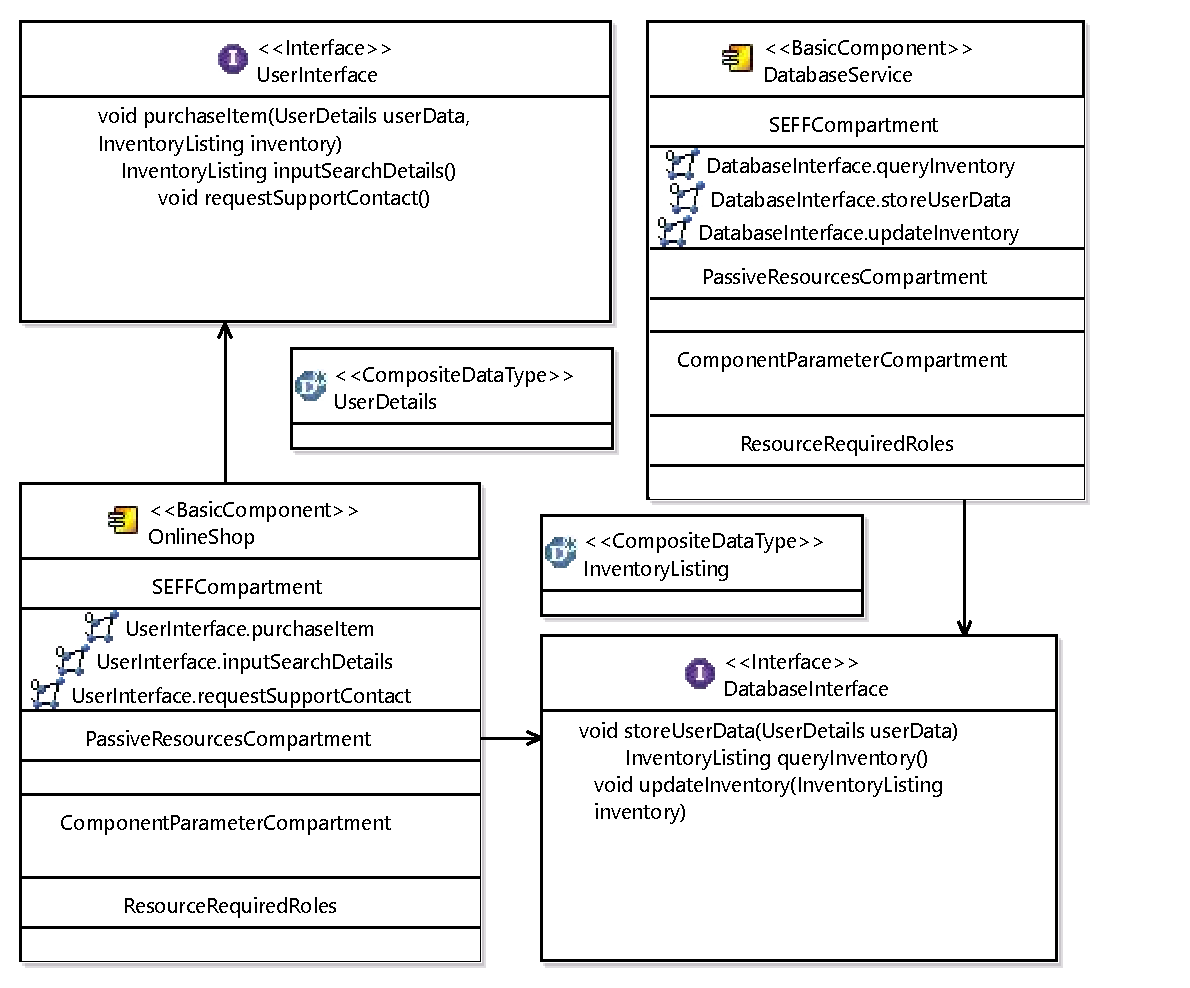
\includegraphics[width=\textwidth]{figures/chapter12/runningexample_repository.pdf}
    \caption[Palladio repository model of the running example.]{Palladio repository model of the running example, exported from the Palladio-Bench \cite{reussner_palladio_2024}.}
    \label{fig:appendix:runningexample:repository}
\end{figure}

\begin{figure}
    \centering
    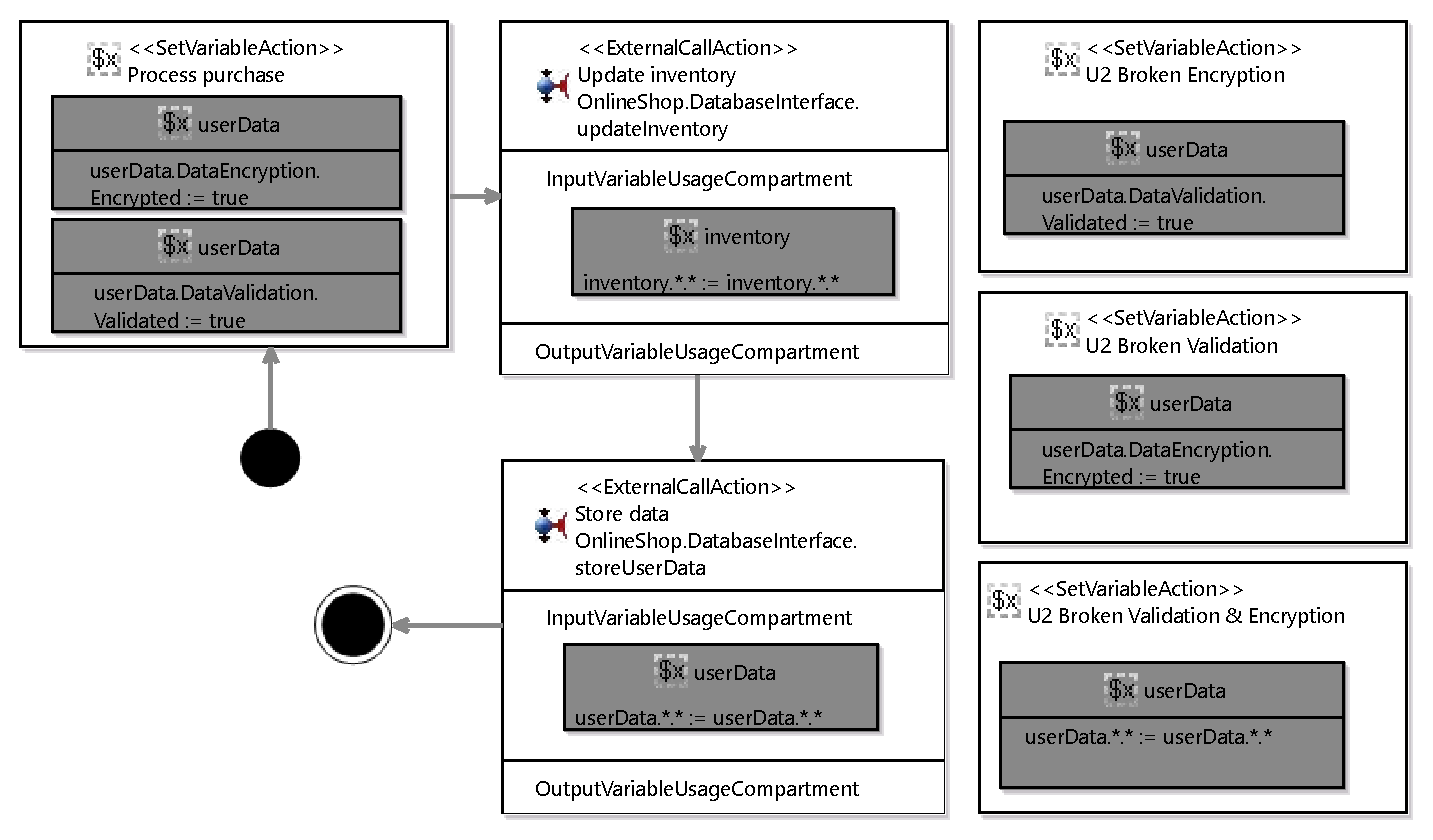
\includegraphics[width=\textwidth]{figures/chapter12/runningexample_seff.pdf}
    \caption[Exemplary Palladio \acf*{SEFF} of the running example.]{Exemplary Palladio \acf*{SEFF} of the running example, exported from the Palladio-Bench \cite{reussner_palladio_2024}.}
    \label{fig:appendix:runningexample:seff}
\end{figure}

\begin{figure}
    \centering
    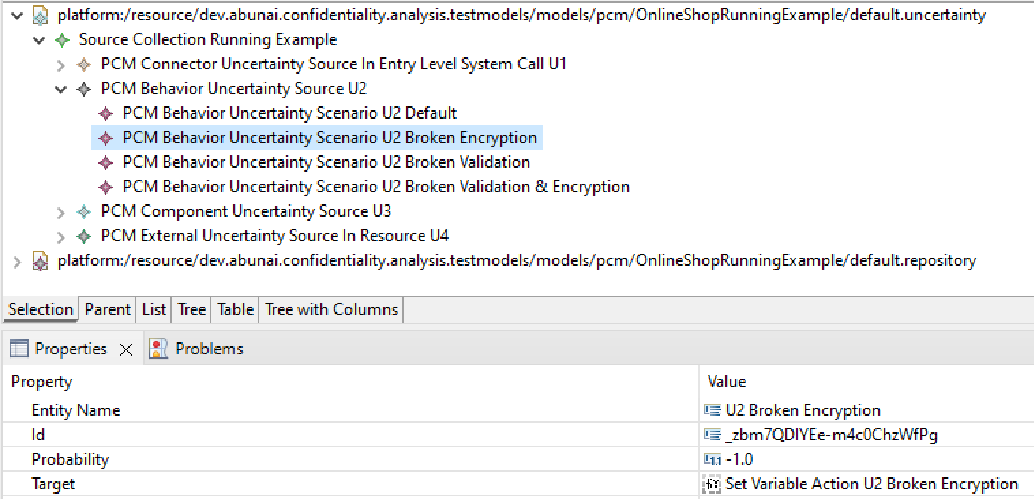
\includegraphics[width=\textwidth]{figures/chapter12/runningexample_uncertainty.pdf}
    \caption[Uncertainty model of the running example, showing four uncertainty sources and their scenarios.]{Uncertainty model of the running example, showing four uncertainty sources and their scenarios. Screenshot from the Palladio-Bench \cite{reussner_palladio_2024}.}
    \label{fig:appendix:runningexample:uncertainty}
\end{figure}





\chapter{Impact Sets of the Running Example}%
\label{sec:appendix:impactset}

Our uncertainty impact analysis has been introduced in \autoref{ch:impactanalysis}.
We show the resulting impact sets after the architectural propagation and the propagation in the \acf{DFD} of the running example, see \autoref{ch:runningexample}.
These are the results of the automated uncertainty impact analysis \uia.
\autoref{lst:appendix:impactset:u1} shows the impact set of Uncertainty \U{1}, \autoref{lst:appendix:impactset:u2} shows the impact set of Uncertainty \U{2}, \autoref{lst:appendix:impactset:u3} shows the impact set of Uncertainty \U{3}, and \autoref{lst:appendix:impactset:u4} shows the impact set of Uncertainty \U{4}.
We removed the element IDs from the analysis output for the sake of brevity.
The comprehensive analysis output can be found in the data set \cite{dataset}.

\begin{figure}
    \begin{lstlisting}[
        style=appendix,
        caption={Result of the uncertainty impact analysis of Uncertainty \U{1} in the running example.},
        label={lst:appendix:impactset:u1}
    ]
    Result of the PCM propagation:
    SEFFActionSequenceElement (Beginning view)
    SEFFActionSequenceElement (Beginning buy)
    SEFFActionSequenceElement (Beginning requestSupport)
    SEFFActionSequenceElement (Beginning view)
    CallingUserActionSequenceElement / calling (ViewEntryLevelSystemCall)
    CallingUserActionSequenceElement / returning (ViewEntryLevelSystemCall)
    CallingUserActionSequenceElement / calling (BuyEntryLevelSystemCall)
    CallingUserActionSequenceElement / returning (BuyEntryLevelSystemCall)
    CallingUserActionSequenceElement / calling (RequestSupportCall)
    CallingUserActionSequenceElement / returning (RequestSupportCall)
    CallingUserActionSequenceElement / calling (ViewShopCall)
    CallingUserActionSequenceElement / returning (ViewShopCall)
    Result of the DFD propagation:
    CallingUserActionSequenceElement / calling (ViewShopCall)
    SEFFActionSequenceElement (Beginning view)
    CallingSEFFActionSequenceElement / calling (DatabaseLoadInventory)
    SEFFActionSequenceElement (Beginning loadInventory)
    SEFFActionSequenceElement (RETURN)
    SEFFActionSequenceElement (Ending loadInventory)
    CallingSEFFActionSequenceElement / returning (DatabaseLoadInventory)
    SEFFActionSequenceElement (RETURN)
    SEFFActionSequenceElement (Ending view)
    CallingUserActionSequenceElement / returning (ViewShopCall)
    UserActionSequenceElement (Stopping usage: View Shop)
    CallingUserActionSequenceElement / calling (ViewEntryLevelSystemCall)
    SEFFActionSequenceElement (Beginning view)
    CallingSEFFActionSequenceElement / calling (DatabaseLoadInventory)
    SEFFActionSequenceElement (Beginning loadInventory)
    SEFFActionSequenceElement (RETURN)
    SEFFActionSequenceElement (Ending loadInventory)
    CallingSEFFActionSequenceElement / returning (DatabaseLoadInventory)
    SEFFActionSequenceElement (RETURN)
    SEFFActionSequenceElement (Ending view)
    CallingUserActionSequenceElement / returning (ViewEntryLevelSystemCall)
    CallingUserActionSequenceElement / calling (BuyEntryLevelSystemCall)
    SEFFActionSequenceElement (Beginning buy)
    SEFFActionSequenceElement (UserDataProcessing)
    CallingSEFFActionSequenceElement / calling (DatabaseStoreInventory)
    SEFFActionSequenceElement (Beginning updateInventory)
    SEFFActionSequenceElement (Ending updateInventory)
    CallingSEFFActionSequenceElement / returning (DatabaseStoreInventory)
    CallingSEFFActionSequenceElement / calling (DatabaseStoreUserData)
    SEFFActionSequenceElement (Beginning storeUserData)
    SEFFActionSequenceElement (Ending storeUserData)
    CallingSEFFActionSequenceElement / returning (DatabaseStoreUserData)
    SEFFActionSequenceElement (Ending buy)
    CallingUserActionSequenceElement / returning (BuyEntryLevelSystemCall)
    UserActionSequenceElement (Stopping usage: Buy from Shop)
    CallingUserActionSequenceElement / calling (RequestSupportCall)
    SEFFActionSequenceElement (Beginning requestSupport)
    SEFFActionSequenceElement (Ending requestSupport)
    CallingUserActionSequenceElement / returning (RequestSupportCall)
    UserActionSequenceElement (Stopping usage: Request Support)
    \end{lstlisting}
\end{figure}

\begin{figure}
    \begin{lstlisting}[
        style=appendix,
        caption={Result of the uncertainty impact analysis of Uncertainty \U{2} in the running example.},
        label={lst:appendix:impactset:u2}
    ]
    Result of the PCM propagation:
    SEFFActionSequenceElement (UserDataProcessing)

    Result of the DFD propagation:
    SEFFActionSequenceElement (UserDataProcessing)
    CallingSEFFActionSequenceElement / calling (DatabaseStoreInventory)
    SEFFActionSequenceElement (Beginning updateInventory)
    SEFFActionSequenceElement (Ending updateInventory)
    CallingSEFFActionSequenceElement / returning (DatabaseStoreInventory)
    CallingSEFFActionSequenceElement / calling (DatabaseStoreUserData)
    SEFFActionSequenceElement (Beginning storeUserData)
    SEFFActionSequenceElement (Ending storeUserData)
    CallingSEFFActionSequenceElement / returning (DatabaseStoreUserData)
    SEFFActionSequenceElement (Ending buy)
    CallingUserActionSequenceElement / returning (BuyEntryLevelSystemCall)
    UserActionSequenceElement (Stopping usage: Buy from Shop)
    \end{lstlisting}
\end{figure}

\begin{figure}
    \begin{lstlisting}[
        style=appendix,
        caption={Result of the uncertainty impact analysis of Uncertainty \U{3} in the running example.},
        label={lst:appendix:impactset:u3}
    ]
    Result of the PCM propagation:
    SEFFActionSequenceElement (Beginning loadInventory)
    SEFFActionSequenceElement (Beginning updateInventory)
    SEFFActionSequenceElement (Beginning storeUserData)
    SEFFActionSequenceElement (Beginning loadInventory)
    
    Result of the DFD propagation:
    SEFFActionSequenceElement (Beginning loadInventory)
    SEFFActionSequenceElement (RETURN)
    SEFFActionSequenceElement (Ending loadInventory)
    CallingSEFFActionSequenceElement / returning (DatabaseLoadInventory)
    SEFFActionSequenceElement (RETURN)
    SEFFActionSequenceElement (Ending view)
    CallingUserActionSequenceElement / returning (ViewShopCall)
    UserActionSequenceElement (Stopping usage: View Shop)
    SEFFActionSequenceElement (Beginning loadInventory)
    SEFFActionSequenceElement (RETURN)
    SEFFActionSequenceElement (Ending loadInventory)
    CallingSEFFActionSequenceElement / returning (DatabaseLoadInventory)
    SEFFActionSequenceElement (RETURN)
    SEFFActionSequenceElement (Ending view)
    CallingUserActionSequenceElement / returning (ViewEntryLevelSystemCall)
    CallingUserActionSequenceElement / calling (BuyEntryLevelSystemCall)
    SEFFActionSequenceElement (Beginning buy)
    SEFFActionSequenceElement (UserDataProcessing)
    CallingSEFFActionSequenceElement / calling (DatabaseStoreInventory)
    SEFFActionSequenceElement (Beginning updateInventory)
    SEFFActionSequenceElement (Ending updateInventory)
    CallingSEFFActionSequenceElement / returning (DatabaseStoreInventory)
    CallingSEFFActionSequenceElement / calling (DatabaseStoreUserData)
    SEFFActionSequenceElement (Beginning storeUserData)
    SEFFActionSequenceElement (Ending storeUserData)
    CallingSEFFActionSequenceElement / returning (DatabaseStoreUserData)
    SEFFActionSequenceElement (Ending buy)
    CallingUserActionSequenceElement / returning (BuyEntryLevelSystemCall)
    UserActionSequenceElement (Stopping usage: Buy from Shop)
    \end{lstlisting}
\end{figure}

\begin{figure}
    \begin{lstlisting}[
        style=appendix,
        caption={Result of the uncertainty impact analysis of Uncertainty \U{4} in the running example.},
        label={lst:appendix:impactset:u4}
    ]
    Result of the PCM propagation:
    SEFFActionSequenceElement (Beginning loadInventory)
    SEFFActionSequenceElement (RETURN)
    SEFFActionSequenceElement (Ending loadInventory)
    SEFFActionSequenceElement (Beginning updateInventory)
    SEFFActionSequenceElement (Ending updateInventory)
    SEFFActionSequenceElement (Beginning storeUserData)
    SEFFActionSequenceElement (Ending storeUserData)
    SEFFActionSequenceElement (Beginning loadInventory)
    SEFFActionSequenceElement (RETURN)
    SEFFActionSequenceElement (Ending loadInventory)

    Result of the DFD propagation:
    SEFFActionSequenceElement (Beginning loadInventory)
    SEFFActionSequenceElement (RETURN)
    SEFFActionSequenceElement (Ending loadInventory)
    CallingSEFFActionSequenceElement / returning (DatabaseLoadInventory)
    SEFFActionSequenceElement (RETURN)
    SEFFActionSequenceElement (Ending view)
    CallingUserActionSequenceElement / returning (ViewEntryLevelSystemCall)
    CallingUserActionSequenceElement / calling (BuyEntryLevelSystemCall)
    SEFFActionSequenceElement (Beginning buy)
    SEFFActionSequenceElement (UserDataProcessing)
    CallingSEFFActionSequenceElement / calling (DatabaseStoreInventory)
    SEFFActionSequenceElement (Beginning updateInventory)
    SEFFActionSequenceElement (Ending updateInventory)
    CallingSEFFActionSequenceElement / returning (DatabaseStoreInventory)
    CallingSEFFActionSequenceElement / calling (DatabaseStoreUserData)
    SEFFActionSequenceElement (Beginning storeUserData)
    SEFFActionSequenceElement (Ending storeUserData)
    CallingSEFFActionSequenceElement / returning (DatabaseStoreUserData)
    SEFFActionSequenceElement (Ending buy)
    CallingUserActionSequenceElement / returning (BuyEntryLevelSystemCall)
    UserActionSequenceElement (Stopping usage: Buy from Shop)
    SEFFActionSequenceElement (Beginning loadInventory)
    SEFFActionSequenceElement (RETURN)
    SEFFActionSequenceElement (Ending loadInventory)
    CallingSEFFActionSequenceElement / returning (DatabaseLoadInventory)
    SEFFActionSequenceElement (RETURN)
    SEFFActionSequenceElement (Ending view)
    CallingUserActionSequenceElement / returning (ViewShopCall)
    UserActionSequenceElement (Stopping usage: View Shop)
    \end{lstlisting}
\end{figure}





\chapter{All Confidentiality Violations in the Running Example}%
\label{sec:appendix:confidentiality}

We give an overview of all confidentiality violations identified in the running example by \abunai.
First, \autoref{lst:appendix:confidentiality:overview} shows all combinations of uncertainty scenarios that cause the violation of at least one confidentiality requirement.
Second, \autoref{lst:appendix:confidentiality:detail} exemplifies the result of the first scenario combination by showing all confidentiality-violating vertices.
The full analysis results can be found in the data set \cite{dataset}.

\begin{figure}
    \begin{lstlisting}[
        style=appendix,
        caption={All uncertainty scenarios of the running example that cause confidentiality violations.},
        label={lst:appendix:confidentiality:overview}
    ]
    [U1 Invalid, U2-Default, U3 Alternative]
    [U1 Invalid, U2 Broken Encryption, U3 Alternative]
    [U1 Invalid, U2 Broken Validation, U3 Alternative] 
    [U1 Invalid, U2 Broken Validation & Encryption, U3 Alternative]
    [U1 Invalid, U2-Default, U3-Default, U4-Default]
    [U1 Invalid, U2-Default, U3-Default, U4 Alternative]
    [U1 Invalid, U2 Broken Encryption, U3-Default, U4-Default]
    [U1 Invalid, U2 Broken Encryption, U3-Default, U4 Alternative]
    [U1 Invalid, U2 Broken Validation, U3-Default, U4-Default]
    [U1 Invalid, U2 Broken Validation, U3-Default, U4 Alternative]
    [U1 Invalid, U2 Broken Validation & Encryption, U3-Default, U4-Default]
    [U1 Invalid, U2 Broken Validation & Encryption, U3-Default, U4 Alternative]
    [U1-Default, U2 Broken Encryption, U3-Default, U4-Default]
    [U1-Default, U2 Broken Encryption, U3-Default, U4 Alternative]
    [U1-Default, U2 Broken Validation & Encryption, U3-Default, U4-Default]
    [U1-Default, U2 Broken Validation & Encryption, U3-Default, U4 Alternative]
    [U1 Invalid, U2 Broken Encryption, U3-Default, U4-Default]
    [U1 Invalid, U2 Broken Encryption, U3-Default, U4 Alternative]
    [U1 Invalid, U2 Broken Validation & Encryption, U3-Default, U4-Default]
    [U1 Invalid, U2 Broken Validation & Encryption, U3-Default, U4 Alternative]
    [U1 Malicious, U2 Broken Encryption, U3-Default, U4-Default]
    [U1 Malicious, U2 Broken Encryption, U3-Default, U4 Alternative]
    [U1 Malicious, U2 Broken Validation & Encryption, U3-Default, U4-Default]
    [U1 Malicious, U2 Broken Validation & Encryption, U3-Default, U4 Alternative]
    \end{lstlisting}
\end{figure}

\begin{figure}
    \begin{lstlisting}[
        style=appendix,
        caption={Detailed result of the first confidentiality violation of the running example.},
        label={lst:appendix:confidentiality:detail}
    ]
    [U1 Invalid, U2-Default, U3 Alternative] -> 
    {SEFFPCMVertex (Beginning purchaseItem,
    _nGp9cITjEeywmO_IpTxeAg), SEFFPCMVertex (Process purchase, _oEBNYDIXEe-m4c0ChzWfPg),
    CallingSEFFPCMVertex / calling (Update inventory, _yVL18ITkEeywmO_IpTxeAg), 
    CallingSEFFPCMVertex / returning (Update inventory, _yVL18ITkEeywmO_IpTxeAg),
    CallingSEFFPCMVertex / calling (Store data, _11NAEITkEeywmO_IpTxeAg), SEFFPCMVertex 
    (Beginning storeUserData, _oGmXgYTjEeywmO_IpTxeAg), SEFFPCMVertex (Ending 
    storeUserData, _oGmXgoTjEeywmO_IpTxeAg), CallingSEFFPCMVertex / returning (Store 
    data, _11NAEITkEeywmO_IpTxeAg), SEFFPCMVertex (Ending purchaseItem, 
    _nGp9cYTjEeywmO_IpTxeAg), CallingUserPCMVertex / returning (U1 Purchase item 
    Invalid, _UQNBoC1WEe-lUc5YrocPyg), UserPCMVertex (Stopping usage: Buy from Shop, 
    _LPwS4iHdEd6lJo4DCALHMw)},
    \end{lstlisting}
\end{figure}





\chapter{Palladio Repository Model of the Corona Warn App}%
\label{sec:appendix:cwa}

In the following, we show the full Palladio \emph{component repository model} of the \emph{Corona Warn App} evaluation scenario, see \autoref{sec:evaluationscenarios:coronawarnapp}.
Due to the large size of this diagram, we split it into four parts, shown in \autoref{fig:appendix:cwa:1}, \autoref{fig:appendix:cwa:2}, \autoref{fig:appendix:cwa:3}, and \autoref{fig:appendix:cwa:4}.
\autoref{fig:appendix:cwa:overview} gives an overview of the structure.
The original full-sized diagram and all \ac{PCM} model files can be found in the data set \cite{dataset}.

\begin{figure}
    \centering
    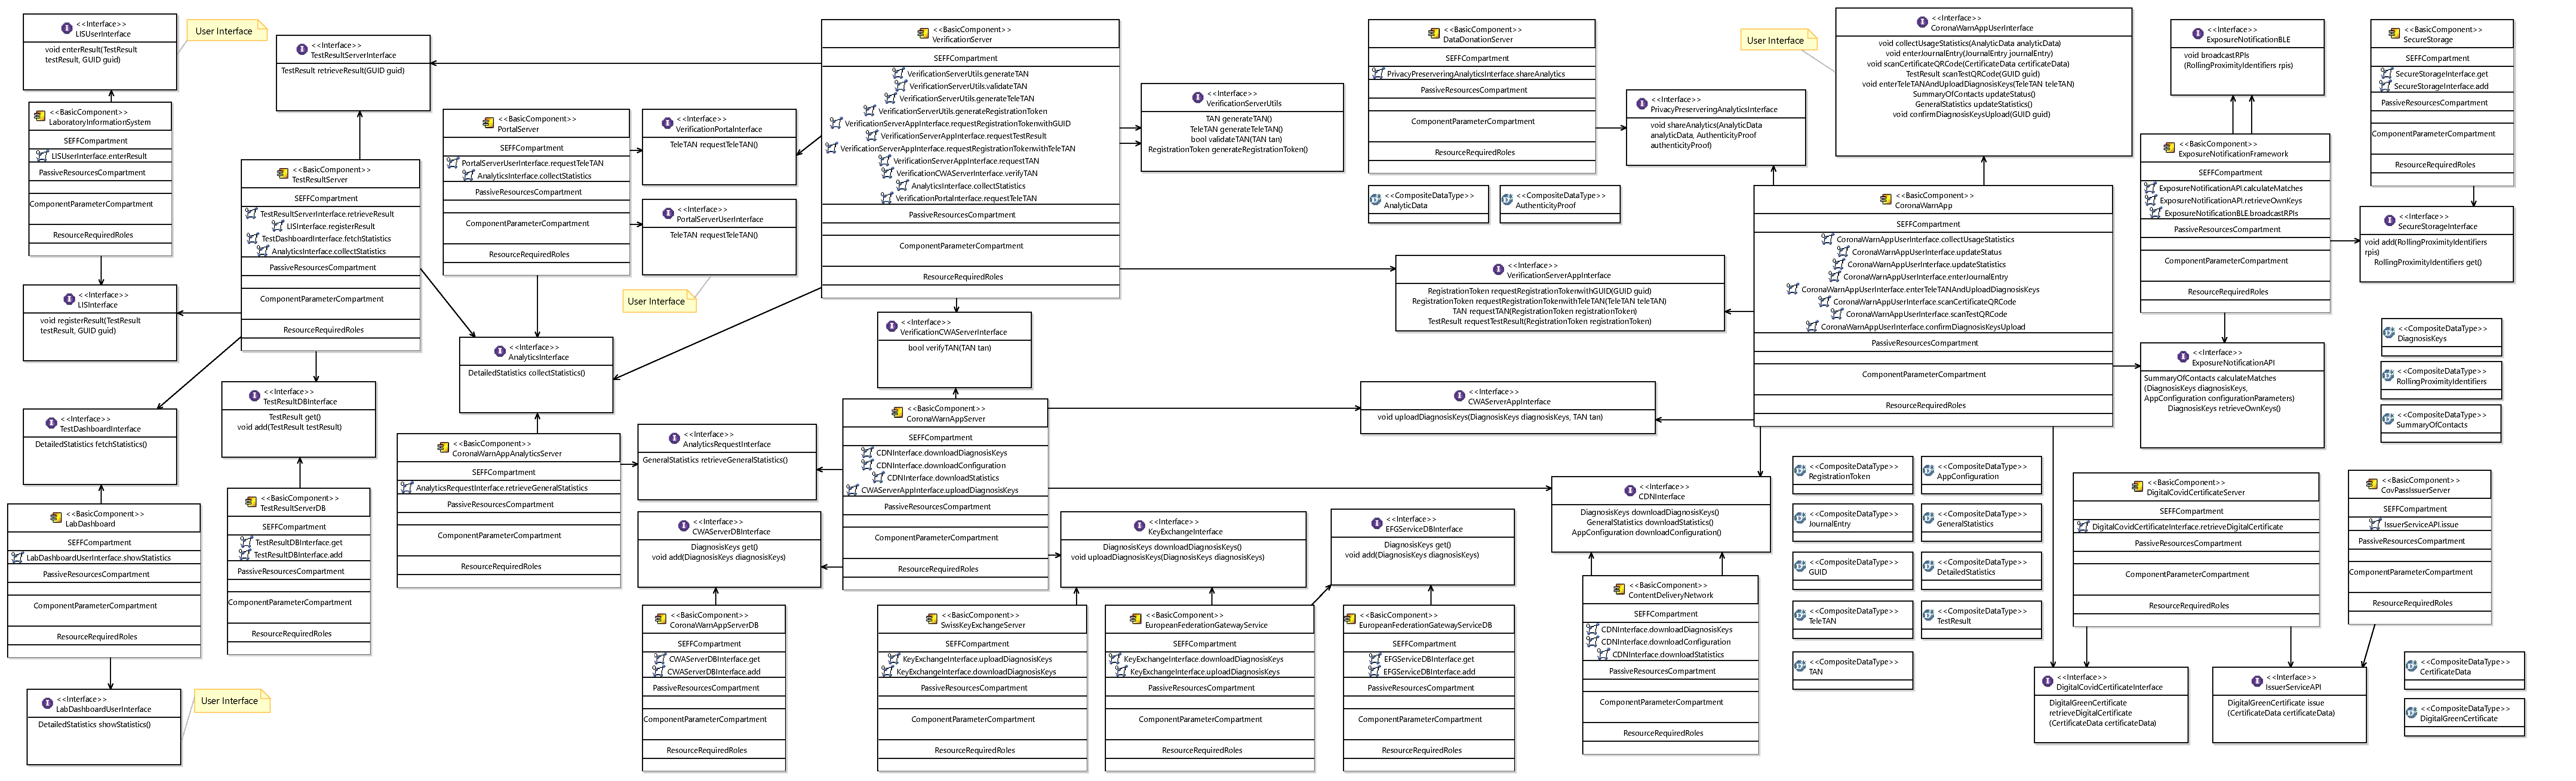
\includegraphics[width=\textwidth]{figures/chapter12/cwa.pdf}
    \caption[Palladio component repository model of the Corona Warn App evaluation scenario (overview).]{Palladio component repository model of the Corona Warn App evaluation scenario (overview), exported from the Palladio-Bench \cite{reussner_palladio_2024}.}
    \label{fig:appendix:cwa:overview}
\end{figure}

\begin{figure}
    \centering
    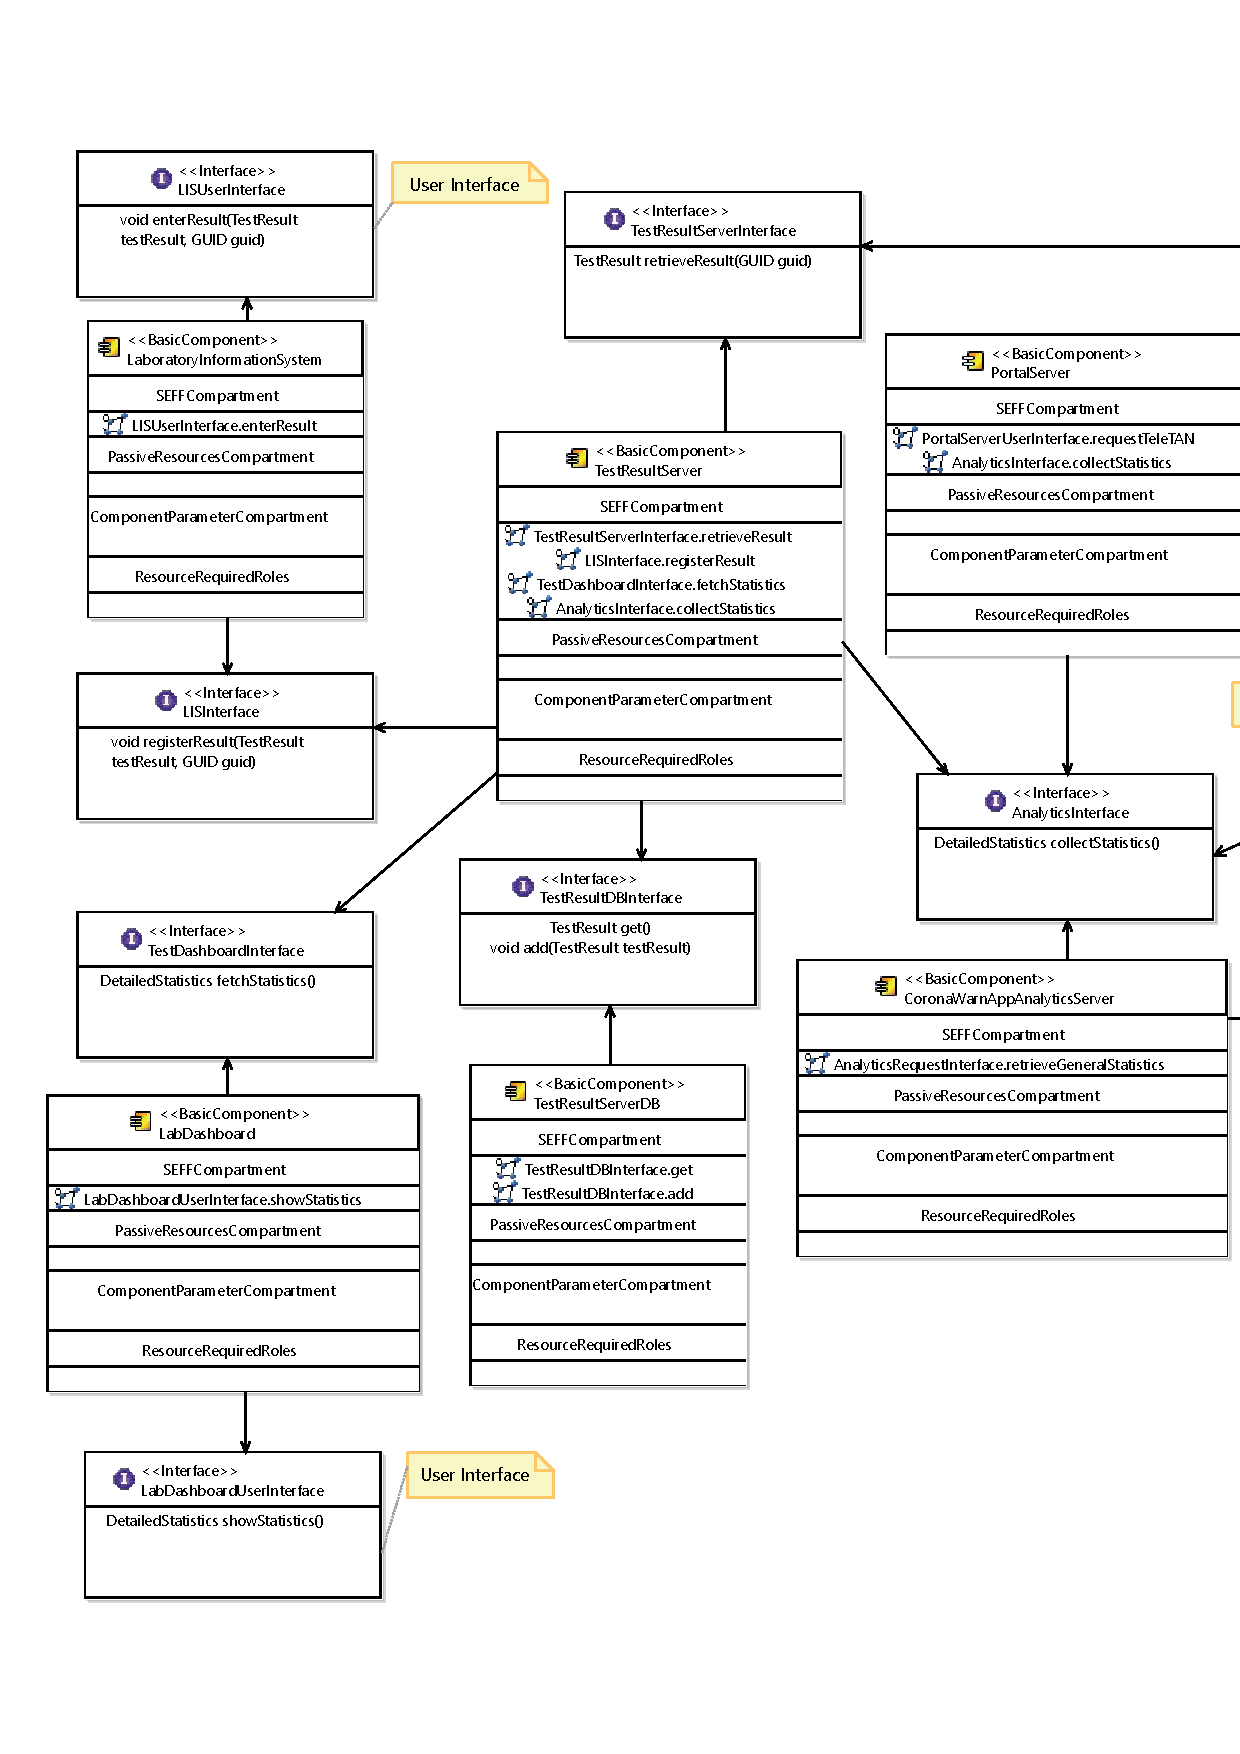
\includegraphics[width=\textwidth]{figures/chapter12/cwa1.pdf}
    \caption[Palladio component repository model of the Corona Warn App evaluation scenario (part 1 of 4).]{Palladio component repository model of the Corona Warn App evaluation scenario (part 1 of 4), exported from the Palladio-Bench \cite{reussner_palladio_2024}.}
    \label{fig:appendix:cwa:1}
\end{figure}

\begin{figure}
    \centering
    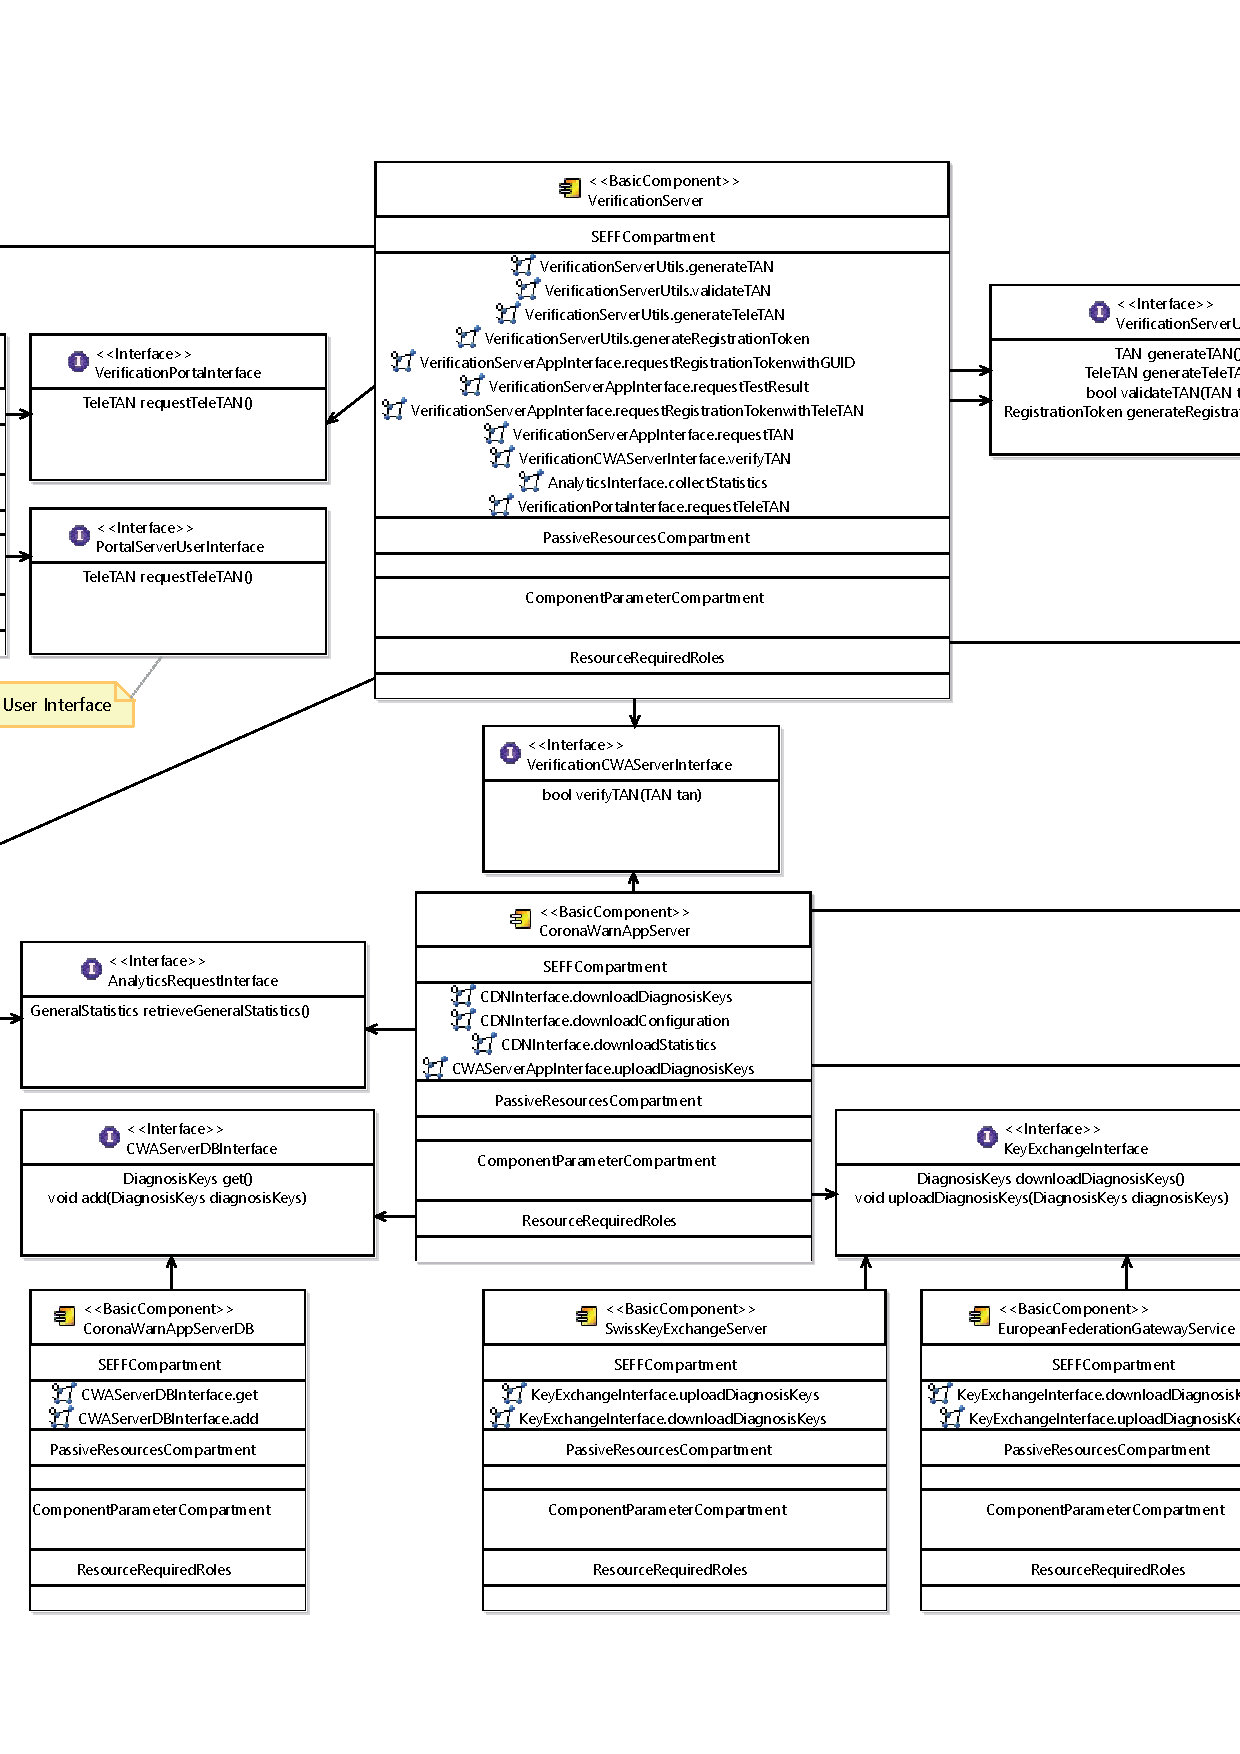
\includegraphics[width=\textwidth]{figures/chapter12/cwa2.pdf}
    \caption[Palladio component repository model of the Corona Warn App evaluation scenario (part 2 of 4).]{Palladio component repository model of the Corona Warn App evaluation scenario (part 2 of 4), exported from the Palladio-Bench \cite{reussner_palladio_2024}.}
    \label{fig:appendix:cwa:2}
\end{figure}

\begin{figure}
    \centering
    \includegraphics[width=\textwidth]{figures/chapter12/cwa3.pdf}
    \caption[Palladio component repository model of the Corona Warn App evaluation scenario (part 3 of 4).]{Palladio component repository model of the Corona Warn App evaluation scenario (part 3 of 4), exported from the Palladio-Bench \cite{reussner_palladio_2024}.}
    \label{fig:appendix:cwa:3}
\end{figure}

\begin{figure}
    \centering
    \includegraphics[width=\textwidth]{figures/chapter12/cwa4.pdf}
    \caption[Palladio component repository model of the Corona Warn App evaluation scenario (part 4 of 4).]{Palladio component repository model of the Corona Warn App evaluation scenario (part 4 of 4), exported from the Palladio-Bench \cite{reussner_palladio_2024}.}
    \label{fig:appendix:cwa:4}
\end{figure}





\chapter{Towards a Graphical Notation for Uncertainty in Data Flow Diagrams}%
\label{sec:appendix:ndfd}

As addressed previously in this dissertation, there is an ongoing discussion on standardizing the representation of uncertainty in software models.
\textcite{troya_uncertainty_2021} conducted a \acf{SLR} on the wide variety of existing proposals on the representation of uncertainty and find that it is a \enquote{good time for the modeling community to try to organize their efforts} \cite{troya_uncertainty_2021}.
This includes a consensus on the types of uncertainty, but also appropriate notations.
In this dissertation, we presented five types of uncertainty sources that are relevant regarding confidentiality and we argued why there should not be less or more than these five types, see \autoref{ch:classification}.
Furthermore, we proposed notations for uncertainty in \acfp{DFD} and \acfp{DAG}, see \autoref{sec:classification:dfd} and \autoref{sec:confidentialityanalysis:abunai}.
However, we did intentionally not define a precise graphical notation, as such an endeavor requires a larger consensus like the ongoing effort to define the \acf{PSUM} standard \cite{PSUM}.
Nevertheless, we want to propose an initial graphical notation for uncertainty in \acp{DFD} that might help the ongoing discussion.

\begin{figure}
    \centering
    \includegraphics[width=0.9\textwidth]{figures/chapter12/graphicalndfd.pdf}
    \caption{Initial proposal for graphically representing uncertainty in \acfp*{DFD}.}
    \label{fig:appendix:ndfd}
\end{figure}

\autoref{fig:appendix:ndfd} shows our proposal.
Regarding the abstract syntax, we use the elements of our meta model for \acfp{NDFD}, see \autoref{fig:confidentialityanalysis:ndfd}.
The graphical representation of \acp{DFD} follows the concrete syntax of the unified modeling primitives by \textcite{seifermann_unified_2021}.
As specified by \textcite{demarco_structure_1979}, nodes are denoted by circles or lines, depending on their type, and flows are denoted by arrows.
In our example, \emph{A} and \emph{B} represent processes and \emph{C} represents a file.
Pins are denoted by rectangles that decouple flows and nodes, and the behavior specified by assignments is annotated to the nodes.
In our example, we show two different behaviors, denoted with different arrow types, e.g., the two-headed arrow $\twoheadrightarrow$.
Last, node labels are also annotated, e.g., \emph{Label A}, and \emph{Label B}.
For an introduction, see \autoref{sec:foundations:dfd}.

Our \ac{NDFD} meta model shows the relation of the five uncertainty types to the \ac{DFD} element types.
\emph{Connector} and \emph{Interface} uncertainty are \emph{secondary} uncertainty types, that affect the flow between nodes, see \autoref{sec:classification:dfd}.
We denote this using the question mark syntax introduced in \autoref{ch:runningexample}, by annotating the question mark to the alternative flow.
In \autoref{fig:appendix:ndfd}, this is shown as an alternative flow to either node \emph{A} or node \emph{B} due to Uncertainty \U{1}.
\emph{Behavior} uncertainty is \emph{primary} uncertainty, directly affecting a node.
We denote this using the question mark and by showing alternative arrows that represent the behavior.
For instance, the behavior of node \emph{A} could be the forwarding or the encryption of data due to Uncertainty \U{2}.
\emph{Component} uncertainty affects a complete node and thus subsumes \emph{Behavior} and \emph{External} uncertainty.
We denote this again using the question mark syntax and show the alternative nodes, e.g., node \emph{A} and node \emph{B} due to Uncertainty \U{3}.
A benefit of this graphical notation is that it shows that both nodes require the same interface, i.e., the same pins.
Last, \emph{External} uncertainty affects node labels.
We denote this using the question mark and by enumerating alternative labels, see Uncertainty \U{4}.

Although this graphical notation has many benefits, e.g., directly representing the different scenarios, it is not perfect yet.
For instance, we cannot represent the difference between \emph{Connector} and \emph{Interface} uncertainty.
Additionally, we cannot represent the impact of \emph{Connector} uncertainty on the assignments of the outgoing node.
Last, to avoid ambiguity, we always have to specify the variation due to the uncertainty, e.g., the different labels, or different behaviors.
Otherwise, the graphical syntax would, e.g., not differentiate between \emph{Behavior} and \emph{External} uncertainty.
Due to these shortcomings, we felt not confident to claim this graphical syntax as part of our contributions.
Instead, we focused on the representation of uncertainty in \acp{DAG} that is more straightforward by only differentiating between \emph{primary} and \emph{secondary} uncertainty.
However, in the light of the recent standardization efforts \cite{PSUM} and to address the need for discussing uncertainty in \acp{DFD} based on drawing diagrams, we conclude this dissertation with this short proposal\footnote{%
\textbf{Acknowledgement}: Not a single sentence of this dissertation was generated by ChatGPT, Gemini, LLaMA, or a comparable tool.
We only used the language-related tools DeepL (\href{https://www.deepl.com/}{https://www.deepl.com/}) and Grammarly (\href{https://grammarly.com/}{https://grammarly.com/}) to correct spelling and grammatical mistakes.}.


\end{document}